% !TeX program = xelatex
\documentclass[UTF8,openany,fontset=fandol,zihao=-4]{ctexbook}
\newcommand{\sdbase}{https://sci-draw.com/zh}
% SPDX-License-Identifier: MIT
\usepackage{fontspec}
\setmainfont{texgyrepagella-regular.otf}[
  BoldFont=texgyrepagella-bold.otf,
  ItalicFont=texgyrepagella-italic.otf,
  BoldItalicFont=texgyrepagella-bolditalic.otf]
\setsansfont{texgyreheros-regular.otf}[
  BoldFont=texgyreheros-bold.otf,
  ItalicFont=texgyreheros-italic.otf,
  BoldItalicFont=texgyreheros-bolditalic.otf]
\setmonofont{lmmono10-regular.otf}[Scale=MatchLowercase]
\usepackage[paperwidth=170mm,paperheight=240mm,inner=20mm,outer=18mm,top=20mm,bottom=22mm,headheight=15pt]{geometry}
\usepackage{graphicx,booktabs,tabularx,longtable,array}
\usepackage{amsmath,amssymb}
\usepackage{enumitem}
\usepackage{xcolor}
\definecolor{BookTeal}{HTML}{176C68}
\definecolor{BookInk}{HTML}{23363E}
\definecolor{BookRule}{HTML}{C8D6D6}
\definecolor{BookPale}{HTML}{F1F6F5}
\usepackage{tikz}
\usetikzlibrary{arrows.meta,positioning,shapes.geometric,shapes.misc,fit,backgrounds,calc,matrix}
\usepackage{rotating}
\usepackage{pdfpages}
\usepackage{fvextra}
\DefineVerbatimEnvironment{Prompt}{Verbatim}{fontsize=\small,breaklines=true,breakanywhere=true,frame=single,rulecolor=\color{BookRule},framesep=2mm}
\usepackage{caption}
\captionsetup{font=small,labelfont=bf,labelsep=period}
\usepackage{fancyhdr}
\pagestyle{fancy}
\fancyhf{}
\fancyhead[LE,RO]{\small\thepage}
\fancyhead[LO,RE]{\small\nouppercase{\leftmark}}
\renewcommand{\headrulewidth}{0.3pt}
\usepackage{xurl}
\usepackage[unicode,hypertexnames=false,colorlinks=true,linkcolor=BookTeal,urlcolor=BookTeal,citecolor=BookTeal,breaklinks=true]{hyperref}
\usepackage{bookmark}
\setcounter{tocdepth}{1}
\setcounter{secnumdepth}{1}
\let\cleardoublepage\clearpage
\setlist{nosep,leftmargin=1.8em}
\renewcommand{\arraystretch}{1.25}
\setlength{\parskip}{0.3em}
\setlength{\emergencystretch}{2em}
\newcommand{\bookversion}{0.1.0}
\newcommand{\bookdate}{2026-10-29}
\newcommand{\scidraw}{SciDraw AI}
% Drawn marks: the book fonts lack U+2713/U+2715.
\newcommand{\bookcheck}{\tikz[x=1em,y=1em,baseline=-0.1em,line width=0.12em,line cap=round,line join=round]\draw[color=.] (0,0.3)--(0.28,0)--(0.75,0.7);}
\newcommand{\bookcross}{\tikz[x=1em,y=1em,baseline=-0.1em,line width=0.12em,line cap=round]{\draw[color=.] (0,0)--(0.6,0.65);\draw[color=.] (0,0.65)--(0.6,0);}}
% Circled numbers and the inhibition sign are missing from the book fonts; draw them.
\usepackage{newunicodechar}
\newcommand{\bookcirc}[1]{\tikz[baseline=(n.base)]\node[circle,draw,inner sep=0.5pt,minimum size=1.05em,font=\sffamily\scriptsize] (n) {#1};}
\newcommand{\bookcircfill}[1]{\tikz[baseline=(n.base)]\node[circle,fill,inner sep=0.5pt,minimum size=1.05em,font=\sffamily\scriptsize\bfseries,text=white] (n) {#1};}
\newunicodechar{①}{\bookcirc{1}}
\newunicodechar{②}{\bookcirc{2}}
\newunicodechar{③}{\bookcirc{3}}
\newunicodechar{④}{\bookcirc{4}}
\newunicodechar{⑤}{\bookcirc{5}}
\newunicodechar{⑥}{\bookcirc{6}}
\newunicodechar{⑦}{\bookcirc{7}}
\newunicodechar{⑧}{\bookcirc{8}}
\newunicodechar{⑨}{\bookcirc{9}}
\newunicodechar{⑩}{\bookcirc{10}}
\newunicodechar{⑪}{\bookcirc{11}}
\newunicodechar{⑫}{\bookcirc{12}}
\newunicodechar{⑬}{\bookcirc{13}}
\newunicodechar{❶}{\bookcircfill{1}}
\newunicodechar{❷}{\bookcircfill{2}}
\newunicodechar{❸}{\bookcircfill{3}}
\newunicodechar{❹}{\bookcircfill{4}}
\newunicodechar{❺}{\bookcircfill{5}}
\newunicodechar{❻}{\bookcircfill{6}}
\newunicodechar{❼}{\bookcircfill{7}}
\newunicodechar{⊣}{\ensuremath{\dashv}}
\providecommand{\sdbase}{https://sci-draw.com}
\newcommand{\sdtool}[1]{\href{\sdbase/#1}{\texttt{/#1}}}
\newcommand{\bookrepo}{https://github.com/TopLocalAI/ai-scientific-figures-book}
\newenvironment{BookNote}{\begin{quote}\small\color{BookInk}}{\end{quote}}
\newcolumntype{Y}{>{\raggedright\arraybackslash}X}
\newcommand{\workflowfigure}[2]{%
  \begin{figure}[htbp]\centering
  \input{figures/workflow-#1.tex}
  \caption{#2}\label{fig:workflow}
  \end{figure}}
\newcommand{\pairedfigure}[2]{%
  \begin{figure}[htbp]\centering
  \includegraphics[width=\linewidth]{figures/paired-comparison-#1.pdf}
  \caption{#2}\label{fig:paired}
  \end{figure}}

\ctexset{chapter={format=\Large\bfseries,beforeskip=12pt,afterskip=22pt}}
\hypersetup{pdftitle={用 AI 画好科研图：从研究思路到论文配图},pdfauthor={TopLocalAI contributors},pdflang={zh-CN}}
\begin{document}
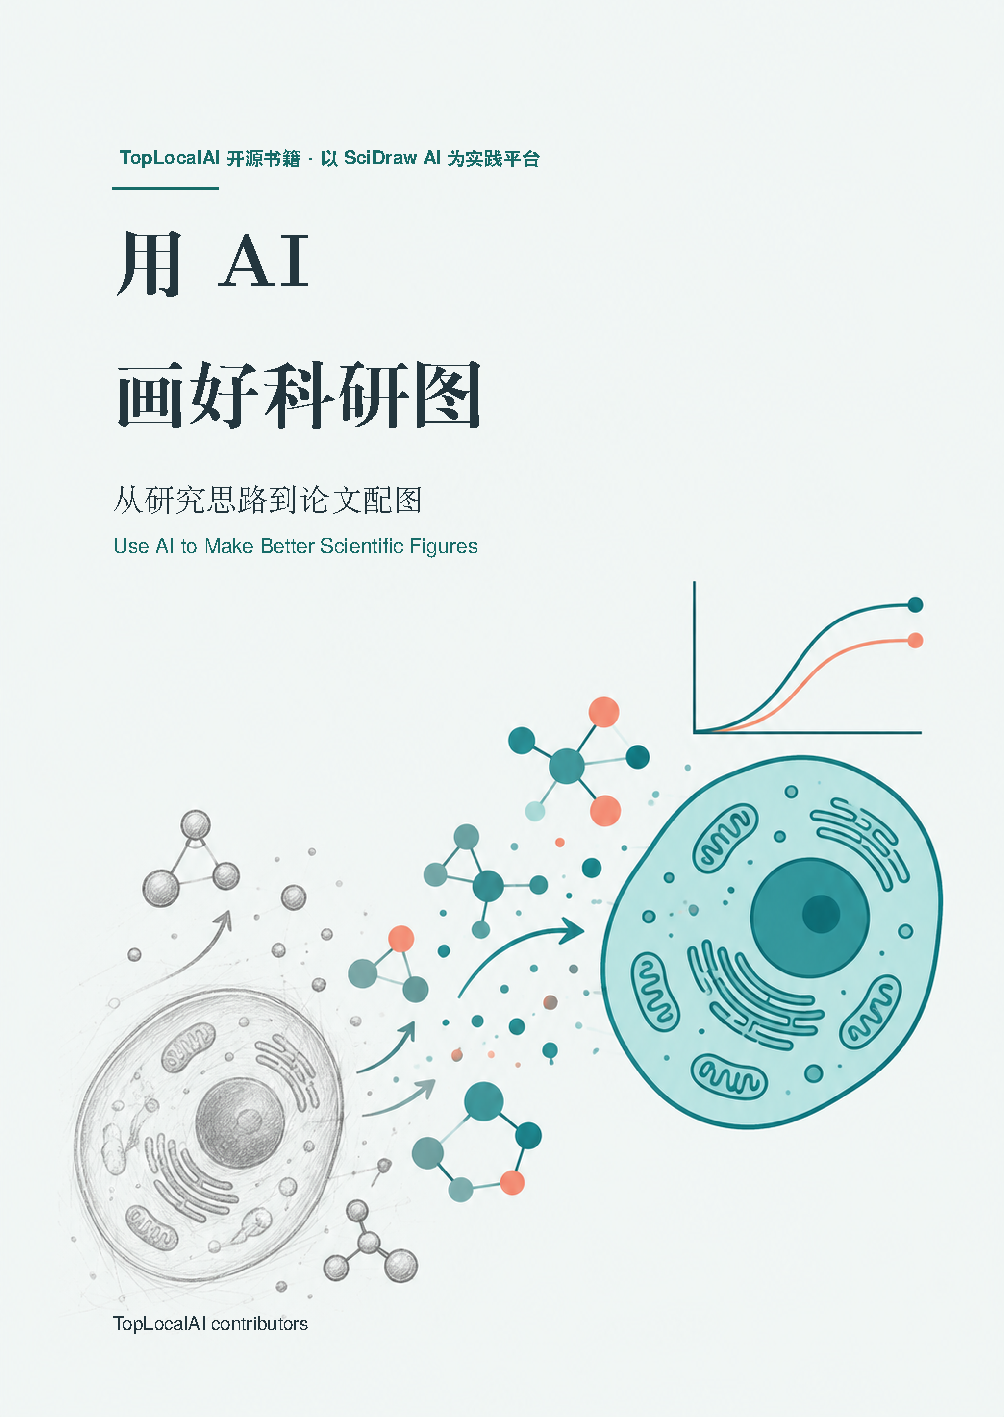
\includepdf[pages=1,fitpaper=false,noautoscale=false]{cover/cover-zh.pdf}
\begin{titlepage}
\color{BookInk}
\vspace*{18mm}
{\sffamily\large TopLocalAI 开源书籍\par}
\vspace{18mm}
{\Huge\bfseries 用 AI 画好科研图\par}
\vspace{8mm}
{\Large 从研究思路到论文配图\par}
\vspace{14mm}
{\large 以 SciDraw AI 为实践平台\par}
\vfill
{\large 中文版 · v\bookversion\par}
\vspace{3mm}
{\normalsize \bookdate\par}
\vspace{8mm}
\end{titlepage}
\frontmatter
\chapter*{版本与使用说明}
本书由 TopLocalAI 开放维护，采用 LaTeX 编写，提供中文和英文两个版本，共十三章，另有前言和附录。

正文以 \scidraw{}（\href{https://sci-draw.com/zh}{sci-draw.com}）组织实践路线。书中提到的工具入口如下，电子版可直接点击：

\begin{center}\small
\begin{tabular}{@{}ll@{}}
提示词绘图、草图、参考图修改 & \href{https://sci-draw.com/zh/ai-drawing}{sci-draw.com/zh/ai-drawing}\\
机制图 & \href{https://sci-draw.com/zh/mechanism-figure-generator}{sci-draw.com/zh/mechanism-figure-generator}\\
流程图 & \href{https://sci-draw.com/zh/workflow-diagram-generator}{sci-draw.com/zh/workflow-diagram-generator}\\
数据可视化 & \href{https://sci-draw.com/zh/sci-vis}{sci-draw.com/zh/sci-vis}\\
组图 & \href{https://sci-draw.com/zh/multi-panel-figure-maker}{sci-draw.com/zh/multi-panel-figure-maker}\\
图形摘要 & \href{https://sci-draw.com/zh/graphical-abstract-maker}{sci-draw.com/zh/graphical-abstract-maker}\\
图注辅助 & \href{https://sci-draw.com/zh/figure-legend}{sci-draw.com/zh/figure-legend}\\
科研绘图向导（串起以上工具） & \href{https://sci-draw.com/zh/figure-workflow}{sci-draw.com/zh/figure-workflow}\\
图片检查 & \href{https://sci-draw.com/zh/figure-checker}{sci-draw.com/zh/figure-checker}\\
\end{tabular}
\end{center}

书中的示意图例由图像生成模型制作，数据图来自公开数据集或明确标注的模拟数据及可运行脚本；每幅图的实际制作工具、提示词与修改过程记录在本书仓库中。

书稿、原创教学数据和图版按 \href{https://creativecommons.org/licenses/by/4.0/}{CC BY 4.0} 提供；构建脚本、绘图程序与通用排版代码按 MIT 许可证提供。许可范围及素材说明见仓库中的 LICENSE、ASSETS.md 和 provenance 目录。产品名称与商标不因开源而转让。

请引用：TopLocalAI contributors. \emph{用 AI 画好科研图：从研究思路到论文配图}. v\bookversion, \bookdate.

\url{https://github.com/TopLocalAI/ai-scientific-figures-book}
\begingroup\small\linespread{1.0}\selectfont
\setlength{\parskip}{0pt}
\tableofcontents
\endgroup
\chapter*{前言：把注意力放回研究表达}
\addcontentsline{toc}{chapter}{前言}
\markboth{前言}{前言}

写论文时，我们经常在最后阶段才开始认真处理图片。数据已经分析，方法已经写完，结论似乎也很清楚，只差把几张图“画好看”。真正动手后，问题却接连出现：一张图塞不下全部信息，两条箭头容易被误解，几组数据放在一起掩盖了个体差异，屏幕上清晰的文字缩进论文后几乎读不出来。

这些困难与研究本身有关。作图要求我们重新决定：什么最重要，哪些内容属于证据，哪些属于解释，读者应该按什么顺序理解它们。图画不清楚，有时是布局还没有找到，有时则是要表达的问题还没有说清楚。

AI 让制作图片的起点变得更低。我们可以用文字描述一个场景，用草图指定构图，用已有图片解释想改哪里，也可以把数据交给可视化工具，尝试不同的表达方式。许多过去需要反复操作的步骤，如今可以通过一段说明开始。这给科研人员留下了更多比较方案和修正表达的空间。

与此同时，一张完成度很高的图片也更容易掩盖问题。错误的关系可以画得很流畅，遗漏的实验条件可以被整齐的版式遮住，没有依据的结论也可能配上一套看似专业的图形语言。我们需要学会把“能生成”进一步推进到“能解释、能核对、能交付”。

本书围绕这一过程展开。你将从一份绘图任务书开始，决定图的用途和核心问题，再选择数据图、方法图、机制图、实验图像或图形摘要的工作路线。我们会讨论构图、颜色、标签和图注，也会花时间处理修改、导出和源文件保存。每一部分都会说明 AI 可以承担哪些工作，以及哪些决定需要你根据研究材料来做。

全书使用 SciDraw AI 作为统一实践平台。统一平台能让读者持续处理同一个案例，减少在不同软件之间重新理解操作的负担。书中介绍的能力以实际界面和可完成的操作为依据；遇到需要下载、上传或人工补充的地方，会直接写出步骤。案例要求的功能尚未具备时，先给出能完成任务的路径，经过实现与实测的功能再进入教程。

你不需要先掌握一套绘画技巧。更有价值的准备，是带上一项熟悉的研究、一份保留完整的材料，以及愿意逐项检查图片的耐心。对科研绘图已经有经验的读者，可以直接从需要解决的问题进入：如何让图表保留研究设计，如何减少机制图中的歧义，如何把多个面板组织成一段可读的论证。

书中的练习会明确区分模拟材料与真实研究。模拟数据让我们能公开复现操作、讨论错误，并且不用把任何教学结果当成科学发现。真实案例则需要可靠来源和必要授权。希望你最终带走的，是一套能应用到自己研究中的工作方法：先确定表达，再使用工具，把每次重要的决定与其依据保留下来。

从下一章开始，请暂时把注意力从“生成一张漂亮图片”移到一个更具体的问题上：这张图要帮助读者理解什么？

\mainmatter
\chapter{建立你的 AI 科研绘图工作流}
\usetikzlibrary{decorations.pathreplacing}

环境科学专业的研究生小林正在撰写一篇关于农业流域河流硝态氮季节变化的论文。论文的第二张图（Figure 2）需要同时交代两件事：一是研究区“农田—地下排水管—支沟—河道—下游监测站”的物质传输路径；二是该站 2016 年全年的每日硝酸盐浓度与河流流量变化。导师看了一眼初稿大纲，只留下一句话：“把一年的监测数据和研究区画成一张图，让人一眼看出浓度跟流量的关系。”

小林立刻打开绘图工具，把从美国地质调查局（USGS）下载的日均值表格传了上去，输入一句：“帮我把这份河流数据画成一张专业的论文图，突出硝酸盐污染问题。”几十秒后，屏幕上出现了一张色彩鲜明、线条饱满的图表（后文图~\ref{fig:ch01-03} 将复现这类典型结果）。初看之下，这张图似乎可以直接放进论文；但准备写图注时，问题接连浮现：左右两条纵轴分别用红绿两色画在同一张图里，曲线交叉处让人误以为浓度与流量“数值相等”；9 月中旬原本有两天仪器缺测，图上却被一条直线直接连了过去；硝酸盐纵轴只写了“mg/L”，没写是按氮原子（以 N 计）还是按硝酸根离子（$\text{NO}_3^-$）计量；10 mg/L 处被画上一条醒目的红线并标着“超标！”，可那其实是针对市政处理后饮用水的标准，并不直接适用于未经处理的河水原水。

接着，她又用一句英文提示词生成研究区示意图（后文图~\ref{fig:ch01-05}）。生成的画面看起来像教科书插图，里面却多出了水处理厂建筑、大片绿色藻华，以及一整套“藻类死亡分解导致溶解氧下降”的生态机制图解——而她的论文既没有测溶解氧，也没有调查水厂。

一句模糊的指令，让工具替作者做出了十几个未经授权的科学决定。本章先解决这个根本问题：在动手输入提示词或运行脚本之前，先把制作科研图片的工作流程建立起来。

\section{给图片一个可以检验的任务}

一张科研图在论文中只承担一个核心任务。这个任务可以是“交代水样从农田进入河道的空间路径”，可以是“展示两个变量在一年十二个月里的同步起伏”，也可以是“比较同一批样本在处理前后的个体变化”。无论具体内容是什么，目标的表述都必须具体到能够直接约束图型、布局和标签。

“展示 2016 年的监测结果”之所以不合格，是因为它无法排除任何错误做法：把 366 天的数据求一个全年均值画成一根柱子，也叫“展示监测结果”；把缺测日悄悄插值补齐、把单位写漏，同样满足“展示监测结果”。相反，如果把任务写成可检验的句子，图的设计边界就立刻清晰起来。

在动笔或打开软件之前，先确定目标读者与核心信息，是科研可视化的基本准则。Rougier 等人（2014）在总结科研作图的十条规则时，把“了解你的读者”和“明确你要传递的信息”排在最前面。本书把这两条规则转化为每一张图开工前必须填写的一句话模板：

\begin{BookNote}
看完这张图，读者应该能够理解\_\_\_\_\_\_\_\_，并能从图中找到\_\_\_\_\_\_\_\_。
\end{BookNote}

前半句规定图片的表达目的，即读者读图后应当建立的整体认识；后半句规定读者可以在画面上逐一指认、核查的具体要素。目标句不需要预先迎合某种“漂亮结论”，相反，它要求图片如实容纳观测到的全部事实。

以小林的河流监测图为例，如果她把这句话写成：

\begin{BookNote}
看完这张图，读者应该能够理解 2016 年 Raccoon River 硝酸盐浓度的季节变化及其与河流流量在时间上的同步关系，并能从图中找到每日均值、缺测日、10 mg/L（以 N 计）参考线以及冬季流量的估算值时段。
\end{BookNote}

单凭这一句话，整张数据图的骨架就已经确定了大半：
\begin{itemize}
\item \textbf{决定图型：}要求读者找到“每日均值”和“缺测日”，意味着不能把数据汇总成月均柱状图或箱线图，必须保留按日排列的时间序列折线，并在缺测日处如实断开，不做平滑滤波或线性插值。
\item \textbf{决定布局：}要求理解浓度与流量“在时间上的同步关系”，同时两者物理量纲完全不同（浓度为 mg/L，流量为 $\text{m}^3/\text{s}$ 且跨越两个数量级），意味着最稳妥的布局是上下堆叠两个共享同一时间横轴的子图，让读者顺着垂直方向比对同一天的峰谷，而不是用容易产生视觉错觉的双 Y 轴把两条线叠在一起。
\item \textbf{决定标签与注释：}句中明确写出“10 mg/L（以 N 计）参考线”和“估算值时段”，直接提醒作者纵轴单位必须标明“以 N 计”，参考线旁必须注明“饮用水标准，仅作参照”，冬季受冰期影响的流量估算值必须在视觉上与实测值区分开来。
\end{itemize}

同样的道理也适用于其他研究设计。例如，当手头是一组样本在实验前后的配对测量值时，如果目标句写的是“理解每个对象在两次测量中的前后变化方向是否一致，并能从图中找到全部对象的配对观测值与逆向变化个体”，那么只画均值和标准差的柱状图就会直接出局，保留个体连线的配对点线图才符合要求（Weissgerber 等，2015）。第 2 章与第 5 章将专门拿这类配对数据拆解从任务定义到统计图表制作的全过程。

当你发现自己很难填完上面那句话的后半格——说不清读者到底应该在图上看到哪些具体元素——通常说明研究思路本身还没有理顺。先停下来把这句话改到可核查，比在绘图工具里盲目尝试二十次提示词更省时间。第 2 章将详细讨论如何把这一句话扩展为完整的绘图任务书。

\section{先判断自己正在处理什么}

写好目标句之后，第二步是清点手头的原始材料。本书从实际操作出发，把制作科研图的材料分成三大类：数值与数据表、解释性内容（文字、草图与已确认的关系）、仪器或现场获取的图像。这是一种面向工具选择与核验责任的操作分类，同一篇论文乃至同一张组合图里，经常同时包含这三类材料。

\begin{center}\footnotesize
\setlength{\tabcolsep}{3pt}
\renewcommand{\arraystretch}{1.15}
\begin{tabularx}{\linewidth}{@{}>{\raggedright\arraybackslash}p{24mm}>{\raggedright\arraybackslash}p{26mm}YY@{}}
\toprule
\textbf{材料类别} & \textbf{图片主要表达什么} & \textbf{本案例对应物与工具路线} & \textbf{作者必须核对什么} \\
\midrule
数值和数据表 & 数量、分布、时间变化与变量关系 & USGS 05484500 站 2016 年日均硝酸盐与流量表；走确定性绘图脚本或 \scidraw{} 科学可视化（\sdtool{sci-vis}）生成面板 b & 原始数值、计量单位、缺测日断开、质量码标记、坐标变换与统计含义 \\
文字、草图与已确认的关系 & 空间结构、实验方法、机制路径与概念解释 & 流域农田地下排水汇入河道及下游监测站位置的文献与站点描述；走 \scidraw{} 生成底图加人工叠字，形成面板 a & 对象增删、数量、水流或作用方向、边界条件，以及是否画出了未支持的污染源或机制 \\
仪器或现场获取的图像 & 实际观测到的形态、条带、显微信号或现场空间信息 & （若研究包含）现场传感器安装照片或遥感影像；保留原始图像，走图像呈现与组图流程（本案例未使用） & 未改动的原始文件备份、比例尺校准、通道与裁切记录、批次可比性，严禁生成式美化 \\
\bottomrule
\end{tabularx}
\end{center}

为什么要先做这道分类题？因为不同材料在论文里承担的\textbf{证据功能}截然不同，对应的制作工具和禁用操作也完全不同（图~\ref{fig:ch01-02}）。

\begin{figure}[htbp]\centering
\resizebox{\linewidth}{!}{\providecommand{\route}[1]{{\scriptsize\color{BookTeal}#1}}
\providecommand{\authcheck}[1]{{\scriptsize\color{BookInk!75}#1}}
\begin{tikzpicture}[
  card/.style={draw=BookTeal,fill=BookPale,rounded corners=2pt,text width=39mm,align=center,font=\small,minimum height=62mm},
  cardunused/.style={card,dashed,draw=gray,text=BookInk!80},
  icon/.style={font=\footnotesize},
  route/.style={font=\scriptsize,text=BookTeal},
  check/.style={font=\scriptsize,text=BookInk!75},
  bracebox/.style={draw=BookInk,rounded corners=1pt,font=\small,inner sep=3pt}
]
\node[card] (d) at (0,0) {%
  \begin{tikzpicture}[scale=0.55,baseline=(t.base)]
    \foreach \x in {0,1,2} {
      \foreach \y in {0,1,2} {
        \draw[BookInk!60] (\x*0.35,\y*0.28) rectangle ++(0.32,0.24);
      }
    }
    \coordinate (t) at (0.35,0.5);
  \end{tikzpicture}\\[2mm]
  数据\\[1mm]
  USGS 日均值\\（硝酸盐、流量）\\[2mm]
  {\route 确定性绘图 / 科学可视化 → 面板 b}\\[2mm]
  {\authcheck 作者核对：原值、单位、缺测、质量码}};
\node[card,right=7mm of d] (i) {%
  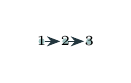
\begin{tikzpicture}[scale=0.55,baseline=(c.base)]
    \foreach \x/\n in {0/1,1/2,2/3} {
      \fill[BookTeal!40] (\x*0.55,0.15) circle (0.07);
      \node at (\x*0.55,0.15) {\tiny\n};
    }
    \draw[-{Stealth},BookInk] (0.07,0.15)--(0.43,0.15);
    \draw[-{Stealth},BookInk] (0.62,0.15)--(0.98,0.15);
    \coordinate (c) at (0.55,0.15);
  \end{tikzpicture}\\[2mm]
  解释性内容\\[1mm]
  研究区与排水路径的文字描述\\[2mm]
  {\route 生成绘图 → 面板 a}\\[2mm]
  {\authcheck 作者核对：对象、方向、是否画出未支持的来源}};
\node[cardunused,right=7mm of i] (p) {%
  
\begin{tikzpicture}[scale=0.55,baseline=(cam.base)]
    \draw[BookInk!70,rounded corners=1pt] (0,0.05) rectangle (0.55,0.38);
    \draw[BookInk!70] (0.55,0.28)--(0.72,0.38)--(0.72,0.05)--(0.55,0.05);
    \fill[BookInk!50] (0.22,0.21) circle (0.09);
    \coordinate (cam) at (0.28,0.21);
  \end{tikzpicture}\\[2mm]
  现场/仪器图像\\[1mm]
  （如有）传感器或采样点照片\\[2mm]
  {\route 原图呈现与组图 → 本案例未使用}\\[2mm]
  {\authcheck 作者核对：原始文件、处理记录}};
\node[font=\scriptsize,text=BookInk!70,anchor=north] at ($(p.south)+(0,-2mm)$) {本例未使用};
\draw[BookInk!50,thick,decorate,decoration={brace,mirror,amplitude=4pt}] ($(d.south west)+(0,-6mm)$) -- ($(p.south east)+(0,-6mm)$);
\node[bracebox,below=9mm of i] (fig) {Figure 2（a \textbar\ b）};
\draw[BookInk!60] (i.south) -- ++(0,-5mm) -| (fig.north);
\draw[BookInk!60] (d.south) -- ++(0,-5mm) -| (fig.north);
\end{tikzpicture}
}
\caption{本章 Figure 2 用到的材料类别。面板 b 是证据，来自数据，走确定性绘图；面板 a 是解释，来自已确认的文字描述，走生成绘图。实验或现场图像属于第三类，本例未使用，第 8 章专门讨论。}\label{fig:ch01-02}
\end{figure}

第一类材料是\textbf{数值和数据表}。数据图在论文中是直接支撑结论的经验性证据。图中每一个点的横纵坐标都必须严格对应数据表里的真实记录，任何平滑、插值、剔除异常值或坐标轴非线性变换（如对数刻度）都直接影响读者的定量判断。因此，数据图必须走确定性绘图路线——无论是编写 Python/R 脚本，还是使用 \scidraw{} 的科学可视化模块（\sdtool{sci-vis}）读取表格并执行绘图代码。绝对不能把数据表或期望的曲线形状塞进纯文生图的图像生成模型里，让模型去“画”一条看起来像折线图的位图；图像生成模型不懂数值映射，它画出的波峰和波谷只是像素拼贴，不是你的观测数据。第 5 章将系统讲解数据图的制作与核验。

第二类材料是\textbf{文字、草图与已确认的关系}。当你需要向读者解释研究区的空间结构、实验步骤的先后顺序或分子生物学中的信号通路时，你手里拿的是文字描述或铅笔草图。由这类材料制作的方法流程图（第 6 章）和机制示意图（第 7 章），其功能是帮助读者理解背景与研究框架，本身不直接充当定量测量证据。在这里，图像生成工具（如 \scidraw{} 的 \sdtool{ai-drawing}、\sdtool{workflow-diagram-generator} 或 \sdtool{mechanism-figure-generator}）可以发挥很大作用：它能根据你的结构描述或草图快速生成构图候选与无文字视觉底图。但解释性图件有一条铁律：\textbf{示意图只能画出你手头材料与文献明确支持的对象和关系，不能“顺手”添加未经证实的因果链条。}在小林的案例中，面板 a 的任务只是交代“农田—地下排水管—支沟—河流—监测站”的监测背景；如果生成模型在河边多画了一座排污工厂或水处理厂，或者在水下画了富营养化耗氧过程，读者就会把右侧面板 b 里的硝酸盐浓度波动归因于那些虚构出来的设施或生态过程。

第三类材料是\textbf{仪器或现场获取的图像}，例如显微镜照片、蛋白印迹（Western blot）、病理切片、电镜图或野外采样点实拍照片。它们和数值表一样，属于原始观测证据。对这类材料，合规的操作仅限于在不改变像素证据的前提下做规范裁剪、对齐、添加校准比例尺、标注通道名称和排版组图（第 8 章）；绝不能把模糊的电泳条带或荧光图像丢进生成式模型里做“超分辨率重绘”或“去噪美化”，那在学术出版规范中属于篡改原始图像。

搞清这三类材料的边界后，面对任何复杂的组合图或图形摘要（第 10 章），你都可以先把它拆成单个面板：哪个面板是数据证据，哪个面板是概念解释，哪个面板是原始影像，各自走各自的制作通道，最后再回到组图工具里合成为一张整图。

\section{把工作分成六个环节}

许多研究生在画论文配图时之所以反复返工，是因为把所有事情混在了一个动作里：一边在对话框里改提示词，一边临时查数据单位，一边猜导师想要什么版式，改了十几轮之后连哪一版对应哪个数据文件都分不清了。

要让作图过程可控，不需要搭建繁琐的软件工程体系，只需把一张图的生命周期固定为六个环节：\textbf{说明任务、准备材料、制作初稿、检查并修改、组织说明、检查与交付}（图~\ref{fig:ch01-01}）。

\begin{figure}[htbp]\centering
\resizebox{\linewidth}{!}{\begin{tikzpicture}[
  box/.style={draw=BookTeal,rounded corners=2pt,fill=BookPale,minimum width=34mm,minimum height=12mm,align=center,font=\small},
  link/.style={-{Stealth[length=2mm]},thick,draw=BookInk},
  loop/.style={-{Stealth[length=1.8mm]},dashed,draw=BookInk!60},
  note/.style={font=\scriptsize,text=BookInk!70,align=center}
]
\node[box] (a) {说明任务};
\node[box,right=9mm of a] (b) {准备材料};
\node[box,right=9mm of b] (c) {制作初稿};
\node[box,below=18mm of c] (d) {检查并修改};
\node[box,left=9mm of d] (e) {组织说明};
\node[box,left=9mm of e] (f) {检查与交付};
\node[note,below=5mm of a] {任务书 v1};
\node[note,below=5mm of b] {数据字典};
\node[note,below=5mm of c] {d1、s1};
\node[note,below=5mm of d] {修改单};
\node[note,below=5mm of e] {组图与图注};
\node[note,below=5mm of f] {交付包};
\draw[link] (a)--(b);
\draw[link] (b)--(c);
\draw[link] (c)--(d);
\draw[link] (d)--(e);
\draw[link] (e)--(f);
\draw[loop] (d.north west) to[bend right=42] (b.south);
\draw[loop] (f.north) to[bend right=48] (a.south);
\node[note,align=center,text width=18mm] at ($(b.south)!0.45!(d.north west)+(0,-10mm)$) {发现问题时返回};
\node[note,align=center,text width=18mm] at ($(a.south)!0.45!(f.north)+(-22mm,2mm)$) {发现问题时返回};
\end{tikzpicture}
}
\caption{本书的六个环节。不适用的环节可以省略；核查发现问题时，返回产生问题的环节，而不是在当前环节反复重画。灰色小字为本章河流硝酸盐案例在各环节留下的产物（其中 d1、s1 分别代表数据面板初稿与示意面板初稿）。}\label{fig:ch01-01}
\end{figure}

这六个环节并不是一条只能硬着头皮往前走的单行道。正如图~\ref{fig:ch01-01} 中两条虚线回路所示，当你在“检查并修改”或“检查与交付”环节发现问题时，最关键的动作是\textbf{判断这个问题究竟产生于哪一个上游环节，然后退回那个环节去修}，而不是停留在当前环节盲目重画。下面逐一说明每个环节的核心工作，以及 AI、确定性工具与作者各自的分工。

\textbf{第一环节：说明任务。}在打开任何生成页面之前，先写清这张图的用途（哪篇论文的第几张图、单栏还是双栏尺寸）、目标读者、那句可检验的目标句、必须包含的对象与关系、视觉与排版约束，以及明确的禁用项和验收条件。AI 可以根据你的初步描述协助梳理栏目并提醒缺项；作者则负责决定研究问题、区分已知事实与假设、敲定验收标准。任务书的写法将在第 2 章展开；草图推演与视觉语言规范将分别在第 3 章和第 4 章展开。

\textbf{第二环节：准备材料。}把作图所需的原始数据表、站点元数据、文献依据或原始实验图像收集到同一个源文件夹中，检查版本一致性，编写简明的数据字典或材料说明。AI 可以协助编写下载与解析脚本、扫描空值与质量码、起草字段说明表；作者必须对照官方参数手册核实物理量单位（如区分“以 N 计”与“以 $\text{NO}_3^-$ 计”），确认采用已审定数据而非临时数据，并锁定未改动的原始文件备份。

\textbf{第三环节：制作初稿。}根据第 1.2 节判定的材料类别，分别进入对应工具生成第一版候选图。数据面板走确定性绘图脚本或科学可视化模块（第 5 章），方法与机制示意走流程图或示意图生成模块（第 6、7 章），实验原图走规范裁剪与标注流程（第 8 章）。AI 与绘图工具负责按明确指令绘制图表或生成无文字示意底图；作者负责把任务书转化为提示词或脚本参数，原样保存每一次实际提交的输入文本，并对候选结果做初步筛选。

\textbf{第四环节：检查并修改。}拿着任务书和数据字典逐条核对初稿，先查科学事实与数据准确性，再查构图、配色与字号，把发现的问题列成结构化的修改单。AI 负责执行具体修改指令；作者负责诊断错误根源并决定退回路径——若发现单位写错或空值被当成 0 读入，应沿图~\ref{fig:ch01-01} 的回路退回“准备材料”修正解析逻辑；若发现把饮用水标准写成了河水“超标”，则应退回“说明任务”厘清概念边界。每次修改后作者都必须对新图做全量复核，尤其检查未要求改动的部分是否被意外改变。第 11 章将专门讲解从初稿到可用稿的分层修改策略。

\textbf{第五环节：组织说明。}多面板组合时，确定网格比例、阅读顺序和面板编号（a、b……），在底图上叠加准确的矢量标签，并编写与图面严格对应的图注。组图工具（\sdtool{multi-panel-figure-maker}）可完成网格排版、编号与尺寸预设，图注辅助工具（\sdtool{figure-legend}）可根据画面起草图注框架；作者则必须补齐画面之外的关键信息（站号、下载日期、换算系数、缺测与估算说明、参考线适用范围），并删去任何未经证实的推测。组图与图注见第 9 章，图形摘要与汇报海报见第 10 章和第 12 章。

\textbf{第六环节：检查与交付。}按目标期刊的实际印刷尺寸（如双栏宽 174 mm）100\% 缩放看图，检查最小字号、线宽、分辨率与色觉可读性，最后将源文件、任务书、草稿、终稿、图注和 AI 使用说明打包归档。图片检查工具（\sdtool{figure-checker}）可自动检测分辨率、色彩模式与对比度风险；作者则负责最终的科学内容核验与投稿合规自查。第 13 章将系统总结核验与交付规范。

\section{一张图从任务书到终稿：河流硝酸盐案例}

现在，我们跟着小林的农业流域河流硝酸盐课题，把上面六个环节完整走一遍。

研究对象位于美国艾奥瓦州中西部的 Raccoon River 流域，该流域以玉米—大豆轮作农田为主，农田下普遍铺设地下排水暗管（tile drainage）。前人对该流域的研究表明，降水与土壤水经地下排水管和基流进入河道，是流域硝态氮输出的主要途径（Schilling 与 Zhang，2004）；原位紫外硝酸盐传感器则使研究者能够以日分辨率连续追踪河水硝酸盐浓度随水文过程的变化（Pellerin 等，2016）。

小林从 USGS 国家水信息系统（NWIS）获取了下游 Van Meter 水文站（站号 05484500）2016 年全年的公开日均值数据。这里必须明确一条科学红线：\textbf{本图只展示 2016 年该站点硝酸盐浓度与河流流量在时间上的共同变化，以及从农田排水到监测站的基本空间关系；本图不作污染来源定量归因，不计算氮负荷，也不作因果推断或显著性检验。}图中引用的美国环保局（EPA）饮用水最大污染物浓度（MCL）10 mg/L（以 N 计），法定适用对象是处理后的公共饮用水，河水原水不适用“超标”表述，图中仅作数值参照。

\textbf{环节一：说明任务——写出可核验的任务书。}吸取了开篇失败尝试的教训，小林先把目标句扩写为一份结构化的绘图任务书，保存在自己课题文件夹的文本文件里，之后在 \scidraw{} 科研绘图向导（\sdtool{figure-workflow}）选定路线、进入各步工具时再把它粘贴进去。以下展示核心栏目，完整提示词见本书仓库（\texttt{cases/} 目录）：

\begin{Prompt}
【用途与读者】环境科学论文 Figure 2，双栏宽 174 mm、高约 110 mm；读者为水文与水质同行。
【目标】理解 2016 年 Raccoon River 硝酸盐浓度的季节变化及其与流量的时间同步关系，
并能从图中找到每日均值、缺测日、10 mg/L（以 N 计）参考线和冰期估算流量时段。
【材料】(1) USGS 05484500 站 2016 年已审定日均值（硝酸盐 mg/L 以 N 计；流量 ft³/s）；
(2) 流域农田与地下排水汇入河道的文献与站点描述（Schilling & Zhang 2004）。
【对象与关系】面板 a（左，约 36% 宽）：农田 → 地下排水管 → 支沟 → 河道 → 监测站；
面板 b（右，约 62% 宽）：上下两个共享月份横轴的子图（上为硝酸盐，下为流量，不画因果箭头）。
【视觉】白底；数据图每子图单色且色觉友好；示意图扁平二维、低饱和、底图禁含任何文字。
【限制】不平滑、不插值、不删观测值；缺测日断开；流量换算为 m³/s 并取对数刻度；
10 mg/L 线仅作参照，不写“超标”；示意图禁画未支持的工厂、排污口、死鱼或藻华。
【验收】363 个硝酸盐日值与 366 个流量日值齐备；3 处缺测断开；极值（5 月 13 日 13.9、
9 月 16 日 3.19）可核查；174 mm 宽印刷时所有文字 >= 6 pt。
\end{Prompt}

这份任务书把设计推演变成了严密的因果链：因为【目标】要求看清每日浓度与流量的同步起伏，而【材料】表明两者单位与量级不同，所以【对象与关系】直接定为“上下两个共享月份横轴的子图”，排除了双 Y 轴；因为【材料】只有单站监测数据与农田排水文献背景，所以【限制】明确禁止画出工厂、排污口或死鱼，并在【验收】里写下了具体的点数（363 与 366）和极值日期（5 月 13 日与 9 月 16 日）。

\textbf{环节二：准备材料——数据字典与三个常见陷阱。}进入第二环节，小林用脚本从 USGS NWIS 日值服务下载了 05484500 站 2016 年原始数据文件（参数码 \texttt{99133} 为原位硝酸盐加亚硝酸盐日均值，参数码 \texttt{00060} 为日均流量，统计码 \texttt{00003} 代表日均；公有领域，引用 DOI 为 \texttt{10.5066/F7P55KJN}），解析为标准 CSV 数据表（\texttt{raccoon-2016-daily.csv}）。先看其中几行关键记录：

\begin{Prompt}
date,nitrate_mgL_as_N,nitrate_qual,discharge_cfs,discharge_qual
2016-01-01,12.1,A,6610,A
2016-01-08,11.1,A,4990,A:e
2016-05-01,8.66,A,16300,A
2016-05-13,13.9,A,10200,A
2016-09-16,3.19,A,5500,A
2016-09-18,,,7110,A
2016-09-19,,,8180,A
2016-12-14,,,968,A:e
\end{Prompt}

同时，她在数据说明文档中整理了数据字典与全表核验值：

\begin{center}\footnotesize
\setlength{\tabcolsep}{3pt}
\renewcommand{\arraystretch}{1.15}
\begin{tabularx}{\linewidth}{@{}l>{\raggedright\arraybackslash}p{26mm}>{\raggedright\arraybackslash}p{28mm}Y@{}}
\toprule
\textbf{字段名} & \textbf{物理含义} & \textbf{单位与编码} & \textbf{2016 年全表核验值} \\
\midrule
\texttt{date} & 日历日期 & \texttt{YYYY-MM-DD} & 共 366 行（闰年） \\
\texttt{nitrate\_mgL\_as\_N} & 原位硝酸盐+亚硝酸盐日均值 & mg/L（以 N 计）；空值为缺测 & 有值 363 天；缺测 3 天（9 月 18—19 日、12 月 14 日）；最大 13.9（5 月 13 日），最小 3.19（9 月 16 日）；$>10\ \text{mg/L}$ 共 162 天；5 月月均最高（12.84），9 月最低（5.36），1 月亦达 11.75 \\
\texttt{nitrate\_qual} & 硝酸盐质量码 & \texttt{A} = 已审定 & 全部为 \texttt{A}，无临时数据 \\
\texttt{discharge\_cfs} & 河道日均流量 & $\text{ft}^3/\text{s}$；乘以 $0.028316846592$ 换算为 $\text{m}^3/\text{s}$ & 366 天全有值；最大 $16,300\ \text{ft}^3/\text{s}$（$\approx 461.6\ \text{m}^3/\text{s}$，5 月 1 日），最小 $411\ \text{ft}^3/\text{s}$（$\approx 11.6\ \text{m}^3/\text{s}$，9 月 6 日） \\
\texttt{discharge\_qual} & 流量质量码 & \texttt{A} = 已审定；\texttt{A:e} = 冰期估算值 & \texttt{A:e} 共 58 天，集中在 1—2 月与 12 月 \\
\bottomrule
\end{tabularx}
\end{center}

这份五列表格里藏着三个必须在数据准备阶段排雷的陷阱：

第一，\textbf{“以 N 计”与“以 $\text{NO}_3^-$ 计”相差 4.43 倍}。硝酸盐浓度既可按氮原子质量报告（mg/L as N，摩尔质量 $14.01\ \text{g/mol}$），也可按完整硝酸根离子报告（mg/L as $\text{NO}_3^-$，摩尔质量 $62.00\ \text{g/mol}$），同一水样后者是前者的 $62.00 / 14.01 \approx 4.43$ 倍。USGS 参数 \texttt{99133} 与美国 EPA 的 10 mg/L 标准均采用“以 N 计”。纵轴标签若漏写“以 N 计”，习惯按 $\text{NO}_3^-$ 读图的同行就会严重误判。

第二，\textbf{流量单位换算与量级跨度}。USGS 原始流量单位是 $\text{ft}^3/\text{s}$，而国际期刊通常使用 $\text{m}^3/\text{s}$。换算改变了图上全部读数（从 $411\text{--}16,300$ 变为 $11.6\text{--}461.6$），且极值相差近 40 倍，属于直接影响读图解释的变换，必须写进档案与图注。

第三，\textbf{缺测日与冰期估算值的保留}。2016 年有 3 天硝酸盐缺测，另有 58 天冬季流量受河冰影响被标为估算值（\texttt{A:e}）。若清洗数据时直接删除含空值的行，那三天的流量也会丢失，折线还会跨过缺测日直接连线；若忽略质量码列，读者就会把冰期估算值当成常规实测值。因此解析脚本必须保留全部 366 行、空值留空，并在作图时把 \texttt{A:e} 日期标出。

在这一环节，AI 可以帮写解析脚本、统计空值与质量码；但对照参数手册确认“以 N 计”、确认未混入临时数据并记录下载日期，必须由作者亲自完成。

\textbf{环节三：制作初稿——数据图的正反对比。}为了看清有无任务书约束的差别，先看只给一句模糊要求时的典型初稿：

\begin{Prompt}
帮我把这份河流数据画成一张专业的论文图，突出硝酸盐污染问题。
\end{Prompt}

缺乏明确的任务约束时，默认绘图脚本或自动可视化很容易生成类似图~\ref{fig:ch01-03} 的问题初稿。

\begin{figure}[htbp]\centering
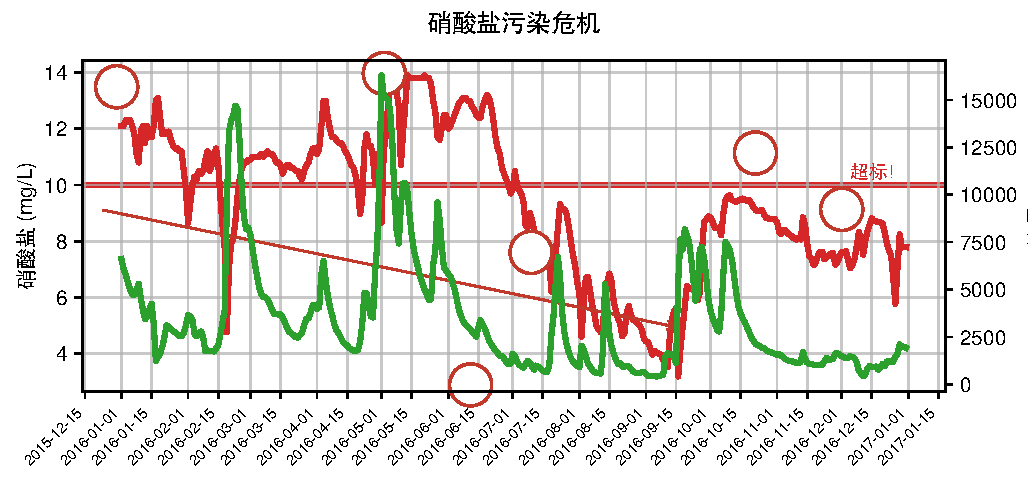
\includegraphics[width=\linewidth]{figures/ch01/ch01-03-nitrate-draft-vague-zh.pdf}
\caption{模糊要求下常见的数据图问题示例（基于真实 USGS 日均值构造的反例）。图中 (1) 双轴与红绿配色、(2) 跨过缺测日的连线、(3) 不完整的单位、(4) 把饮用水参照线写成“超标！”、(5) 带结论的标题、(6) 拥挤的日期刻度，都会让读者误读。}\label{fig:ch01-03}
\end{figure}

对照任务书检查这张初稿，图~\ref{fig:ch01-03} 上用红圈标出的六处硬伤非常清楚：(1) 采用红绿双 Y 轴且右轴未做单位换算，两条曲线的交叉位置随纵轴范围任意移动，极易造成“某日浓度与流量数值相当”的视觉假象，且红绿撞色对色觉障碍读者极不友好；(2) 细箭头所指的 9 月 18—19 日与 12 月 14 日缺测处被绘图函数默认用直线连过，相当于凭空伪造了三天的连续观测值；(3) 左轴漏写“以 N 计”，右轴既无单位也未区分冬季冰期估算值；(4) $y=10$ 处画了刺眼的红实线并标“超标！”，把市政饮用水标准错误套用到未经处理的河水原水上；(5) 顶部冠以“硝酸盐污染危机”的煽动性标题，越俎代庖替读者下结论；(6) 横轴按半月输出完整年月日字符串，字号拥挤越界，浓重的背景网格线反而喧宾夺主。

现在看按任务书约束的做法。在 \scidraw{} 科学可视化（\sdtool{sci-vis}）中上传 \texttt{raccoon-2016-daily.csv} 后，输入如下结构化指令：

\begin{Prompt}
读取上传的 raccoon-2016-daily.csv。date 为日期；nitrate_mgL_as_N 为
硝酸盐+亚硝酸盐日均值（mg/L，以 N 计）；discharge_cfs 为日均流量（ft³/s）。
绘制上下两个共享横轴的子图，不要使用双 Y 轴：
上图：硝酸盐日均值折线；纵轴“硝酸盐（mg/L，以 N 计）”；在 10 处画一条
灰色虚线，旁注“美国 EPA 饮用水 MCL 10 mg/L（以 N 计），仅作参照”。
下图：流量换算为 m³/s（乘以 0.028316846592），纵轴用对数刻度，
标“流量（m³/s，对数刻度）”；discharge_qual 为 A:e 的日期用浅色标出。
数值为空的日期在曲线上断开，不要插值、平滑或删除任何行。
横轴按月标注 2016 年 1–12 月。每个子图只用一种颜色，色觉友好。
不加标题，不加“超标”“污染”等结论性文字。
\end{Prompt}

按上述规则执行确定性绘图后，即可得到规范的数据图面板（图~\ref{fig:ch01-04}）。

\begin{figure}[htbp]\centering
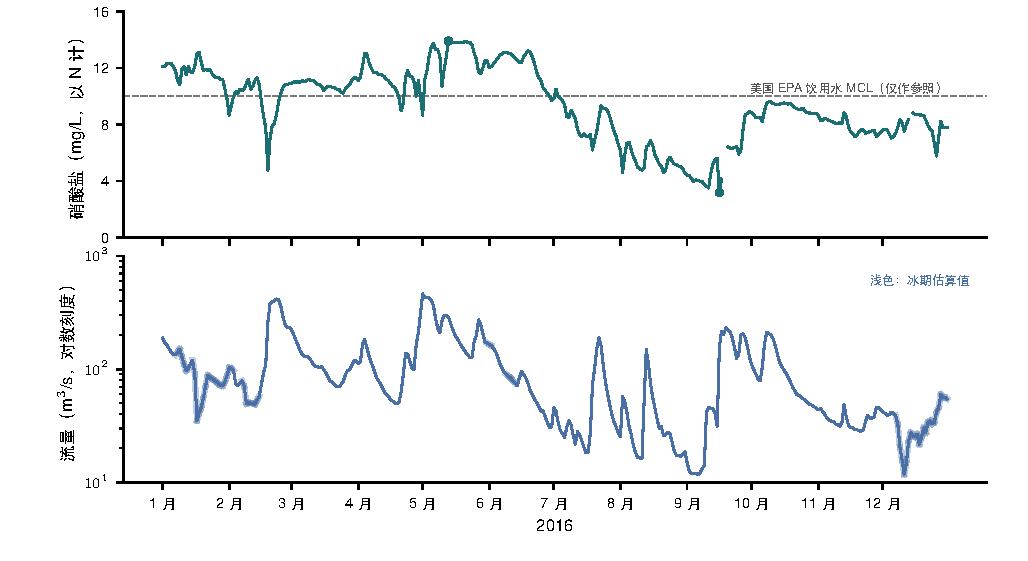
\includegraphics[width=\linewidth]{figures/ch01/ch01-04-nitrate-panel-brief-zh.pdf}
\caption{按任务书重绘的同一份数据。上：硝酸盐+亚硝酸盐日均浓度（mg/L，以 N 计），9 月 18—19 日与 12 月 14 日缺测处断开；灰色虚线为美国 EPA 饮用水最大污染物浓度 10 mg/L，仅作参照，河水原水不适用该标准。下：日均流量，由 $\text{ft}^3/\text{s}$ 换算为 $\text{m}^3/\text{s}$，对数刻度；浅色段为冰期估算值。数据：USGS 05484500，Raccoon River at Van Meter, IA，已审定日均值，2026 年 10 月 29 日下载。}\label{fig:ch01-04}
\end{figure}

对比图~\ref{fig:ch01-04} 与图~\ref{fig:ch01-03}，六处问题全部解决：上下子图共享月份横轴，既消除了双轴交叉错觉，又方便读者顺着垂直方向比对每次涨水过程与硝酸盐浓度的响应；上图在三个缺测日处如实留白断开，并用圆点标出 5 月 13 日全年峰值（13.9 mg/L）与 9 月 16 日谷值（3.19 mg/L）；$10\ \text{mg/L}$ 改为低调的灰色虚线并注明“仅作参照”；下图用对数刻度清晰展开跨越近两个数量级的流量变化，并用浅色宽线标出 58 天冰期估算值。从图上还能如实读出一个重要事实：2016 年虽然在 5 月出现最高月均浓度（12.84 mg/L）、9 月最低（5.36 mg/L），但 1 月份浓度同样处于高位（月均 11.75 mg/L）。只有拒绝平滑滤波与偏向性标题，才能让这些真实的季节特征完整呈现出来。

\textbf{环节三（续）：制作初稿——研究区示意图的正反对比。}接下来制作面板 a 的研究区示意图。同样先看只给一句模糊要求时会发生什么。如果向图像生成工具只输入一句宽泛的英文提示词：

\begin{Prompt}
Illustration of nitrate pollution in an agricultural river watershed. Aspect ratio 4:3.
\end{Prompt}

很多人以为模糊提示词的主要风险是生成扭曲的伪文字或冒烟的工厂烟囱。但我们把同一提示词连续生成了三次，结果给出了一个更值得警惕的教训：三次生成都没有出现工业烟囱或死鱼，图中的英文说明框和方向箭头也基本可读；然而模型为了诠释“污染（pollution）”，自作主张地塞进了大量\textbf{本案例材料根本没有支持的设施与生态机制}。图~\ref{fig:ch01-05} 是三次生成中的代表性结果，图中红圈 1—4 标出了画面中出现的四处问题。

\begin{figure}[htbp]\centering
\begin{tikzpicture}
\node[anchor=south west,inner sep=0] (img) at (0,0) {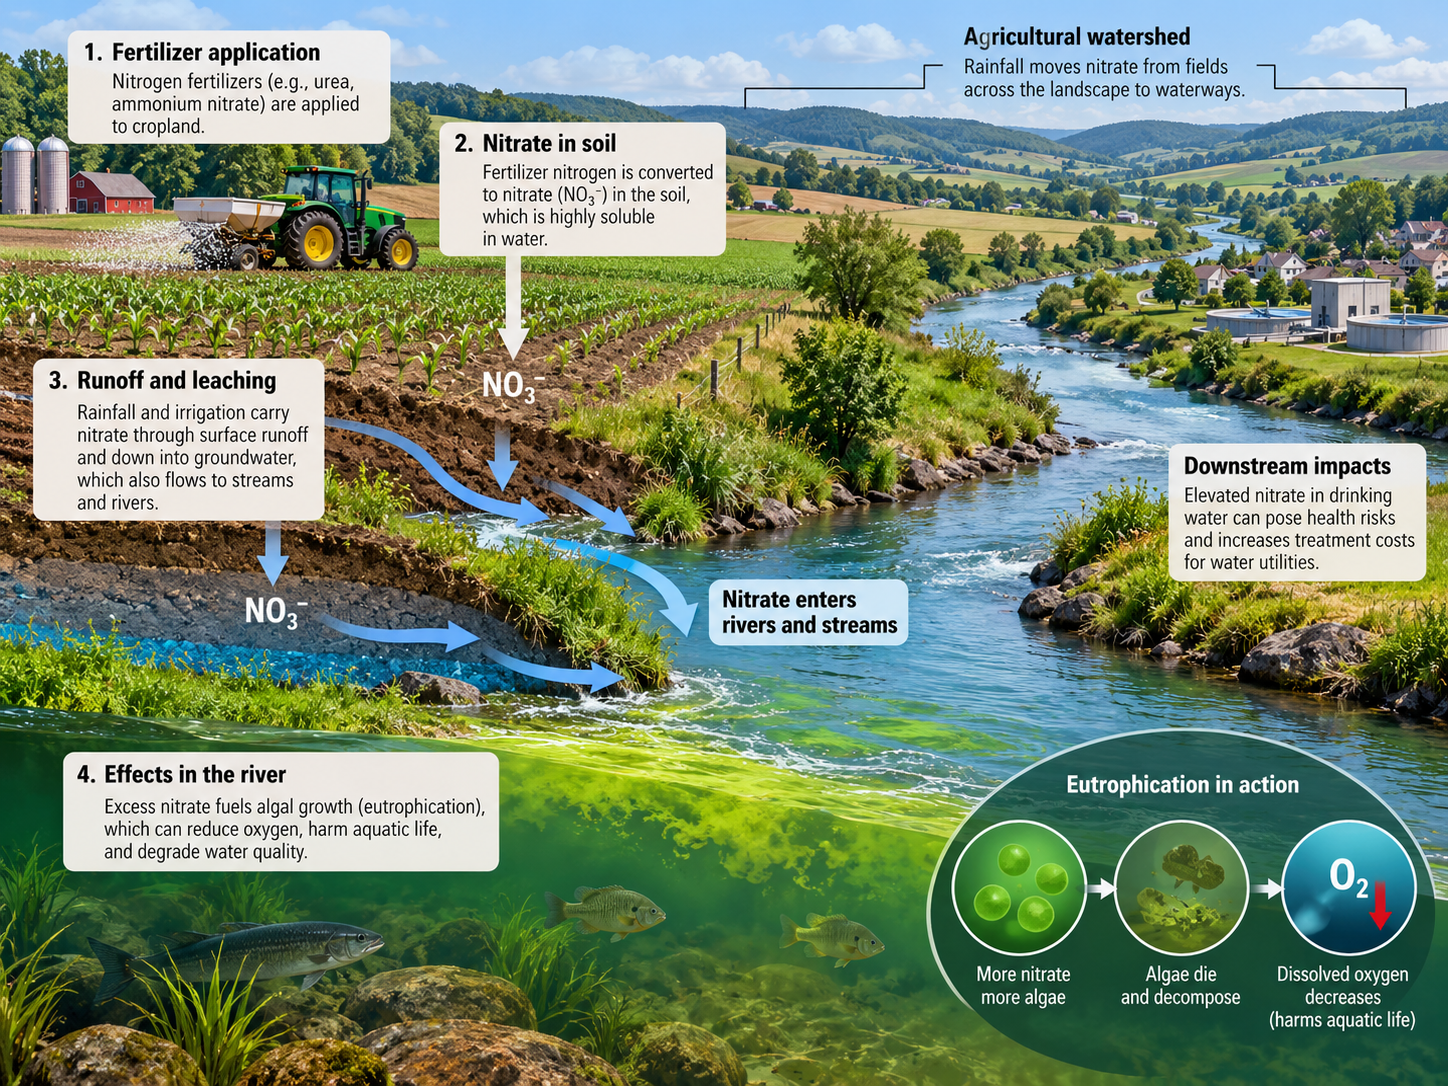
\includegraphics[width=\linewidth]{figures/ch01/ch01-05-site-schematic-vague.png}};
\begin{scope}[x={(img.south east)},y={(img.north west)}]
  \tikzset{badmark/.style={draw=red!80!black,very thick,circle,fill=white,fill opacity=0.88,text opacity=1,text=red!80!black,font=\bfseries\small,inner sep=1.2pt}}
  \node[badmark] at (0.88,0.72) {1};
  \node[badmark] at (0.80,0.22) {2};
  \node[badmark] at (0.22,0.80) {3};
  \node[badmark] at (0.62,0.45) {4};
\end{scope}
\end{tikzpicture}
\caption{用一句模糊要求生成的研究区示意图（本章示例图由图像模型生成，提示词与生成记录见本书仓库）。模型虽未生成工业排污烟囱或乱码，却加入了本案例材料并不支持的内容：(1) 右岸的水处理设施样建筑、聚落及饮用水处理成本说明，(2) 近景藻华、水下鱼群与右下角“富营养化—藻类分解—溶解氧下降”机制图解（同时漏掉了关键的农田地下排水管），(3) 写实风景、水下摄影透视与直接烧录在位图中的大段英文说明框，(4) 虽有径流箭头但缺少下游 USGS 监测站与传感器位置。}\label{fig:ch01-05}
\end{figure}

逐一核对这四处具体问题：
\begin{itemize}
\item \textbf{问题 (1)（未支持的水处理设施与成本说明）：}右岸（红圈 1）画出了聚落、带两个圆形池体的水处理设施样建筑，并配文讨论饮用水风险与水厂处理成本。本案例没有任何水厂位置或处理成本的数据，画入研究区面板会误导读者。
\item \textbf{问题 (2)（越界的富营养化机制与漏画排水管）：}近景与右下角（红圈 2）画出了大片绿色藻华、水下鱼群，以及“硝酸盐增加 $\rightarrow$ 藻类死亡分解 $\rightarrow$ 溶解氧（$\text{O}_2$）下降”的因果图解；而左侧土壤剖面只画了地表径流与地下水，反而漏掉了本流域最关键的农田地下排水管。把未测量的下游生态效应画成既定事实、同时漏掉核心传输通道，属于严重的科学失真。
\item \textbf{问题 (3)（写实装饰风格与锁死在位图中的文字）：}画面（红圈 3）采用写实天空、拖拉机远景与水下光影，且四个大段英文说明框直接烧录在位图里，字号、字体与语言均无法在后期单独修改。
\item \textbf{问题 (4)（缺少监测站位置）：}图中虽有径流箭头，但下游（红圈 4）没有标出 USGS 05484500 监测站与原位传感器，无法与面板 b 的数据建立空间对应。
\end{itemize}

要把示意图拉回正轨，核心是两条：一是明确列出\textbf{必须出现的科学对象}与\textbf{严格排除清单}；二是要求模型\textbf{只输出不含任何文字的干净底图}，文字标签留到后期在组图或矢量工具中单独叠加。修改后的结构化英文提示词关键部分如下（完整提示词见本书仓库 \texttt{cases/} 目录）：

\begin{Prompt}
Flat 2D scientific schematic for a journal figure panel, portrait 4:5, pure white
background. Clean vector style: flat fills, thin dark-gray outlines, no gradients,
no shadows, no 3D, no texture.
ABSOLUTELY NO TEXT: no letters, words, numbers, symbols, labels, legend, or title.
SCENE: simplified oblique (~30-degree) view of an agricultural landscape with a
cut-away soil block in the lower-left quarter.
- Upper half: 5-6 rectangular fields in muted sage green and wheat yellow; no buildings.
- Meandering river (soft blue) from upper-left to lower-right, joined by one tributary ditch.
- Lower-left soil cut-away: 3 round gray subsurface drain pipes, one outlet discharging
  into the tributary ditch.
- Lower-right river bank: simple gray monitoring station box with cable to a submerged
  cylindrical sensor; 2-3 hollow chevrons on water surface pointing downstream.
STRICTLY EXCLUDE: factories, chimneys, sewage pipes, towns, bridges, dead fish, algae,
murky water, warning signs, chemical symbols, clouds, decorative borders.
\end{Prompt}

即便提示词如此细致，生成结果仍需逐张核验筛选。我们把同一提示词生成了三次，结果各有差异：第 1 次生成中，左下角土壤剖面的受水沟与汇入主河道的支沟之间出现白色断口，“排水管 $\rightarrow$ 支沟 $\rightarrow$ 主河道”的水流路径被截断，因此淘汰；第 3 次生成画出了两条独立支沟分别汇入主河道，偏离了“单条支沟汇入”的设定，同样淘汰；只有第 2 次生成完整实现了白底、零文字、6 块农田、3 个灰色排水管口、连续汇入主河道的支沟、下游岸边的监测站与水下传感器，以及 3 个指向下游的白色 V 形流向标记，且排除清单中的干扰物均未出现。

把第 2 次生成图放大到 200\% 仔细核对，仍能看到四处细微偏差：支沟在入河前呈小 Y 形合流；右侧第三个排水管口直接兼作出水口；传感器停在水面波纹处而未完全画成深水浸没；土壤剖面与仪器箱体仍带轻微颗粒纹理和明暗过渡。由于这些细节不影响“农田—地下排水管—支沟—主河道—监测站”的核心空间拓扑，且画面干净无伪文字，可以在图注中注明“简化示意，不按比例”，再在预留的空白处叠加六个中文矢量标签，得到合格的研究区示意面板（图~\ref{fig:ch01-06}）。

\begin{figure}[htbp]\centering
\begin{tikzpicture}
\node[anchor=south west,inner sep=0] (img) at (0,0) {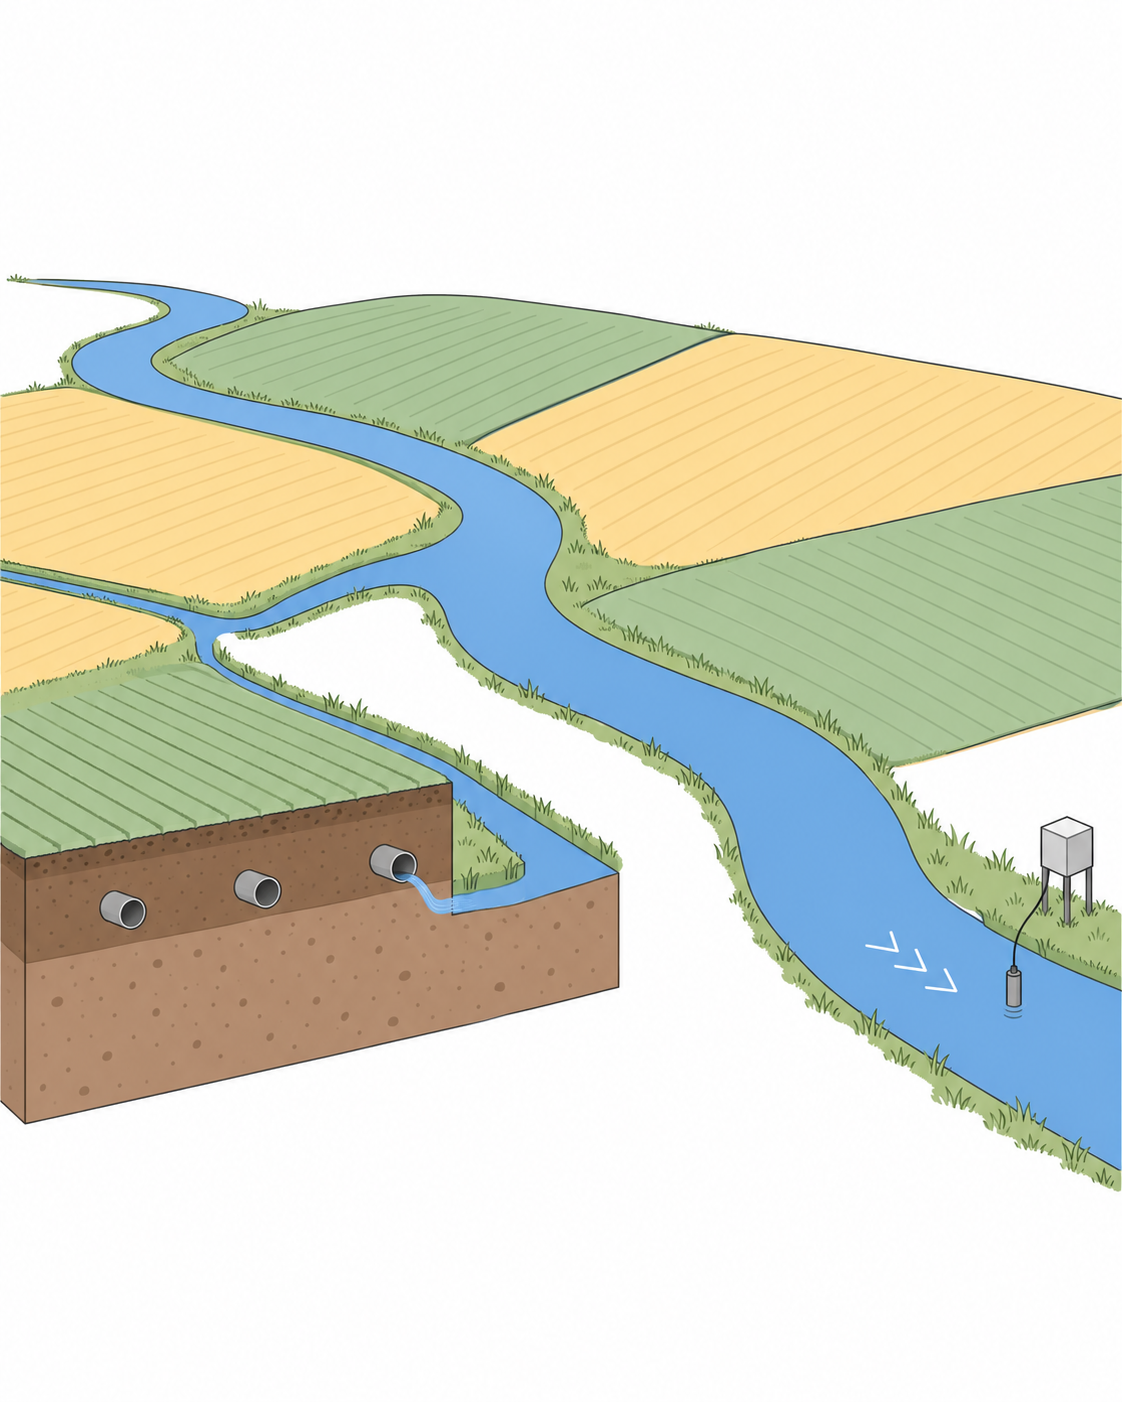
\includegraphics[width=0.62\linewidth]{figures/ch01/ch01-06-site-schematic-brief.png}};
\begin{scope}[x={(img.south east)},y={(img.north west)}]
  \tikzset{lbl/.style={font=\footnotesize,fill=white,fill opacity=0.82,text opacity=1,inner sep=1.5pt,align=center}}
  \node[lbl] at (0.50,0.88) {农田（玉米—大豆，示意）};
  \node[lbl] at (0.22,0.18) {地下排水管};
  \node[lbl] at (0.12,0.45) {支沟};
  \node[lbl] at (0.55,0.55) {Raccoon River};
  \node[lbl] at (0.80,0.12) {监测站 USGS 05484500};
  \node[lbl] at (0.72,0.36) {水流方向};
\end{scope}
\end{tikzpicture}
\caption{按任务书生成的研究区示意底图（三次生成中的第 2 次结果）及后期叠加的中文标签。底图不含任何生成文字，排除了无关设施与未证实的生态后果，清晰交代“农田—地下排水管—支沟—主河道—下游监测站”的空间关系。}\label{fig:ch01-06}
\end{figure}

\textbf{环节四：检查并修改——用修改单管理迭代。}面对初稿中的问题，不能只说“再改得专业一点”，而应将数据图初稿（图~\ref{fig:ch01-03}）与示意图初稿（图~\ref{fig:ch01-05}）的问题逐条对照任务书列成\textbf{修改单}，明确具体修改指令及退回环节：

\begin{center}\footnotesize
\setlength{\tabcolsep}{3pt}
\renewcommand{\arraystretch}{1.15}
\begin{tabularx}{\linewidth}{@{}c>{\raggedright\arraybackslash}p{32mm}>{\raggedright\arraybackslash}p{20mm}Y>{\raggedright\arraybackslash}p{22mm}@{}}
\toprule
\textbf{\#} & \textbf{初稿中发现的问题} & \textbf{违反的条款} & \textbf{可核查的修改指令} & \textbf{应退回的环节} \\
\midrule
1 & 双 Y 轴，两线交叉让人误以为“浓度与流量相等” & 【对象与关系】 & 拆为上下两个共享横轴的子图 & 制作初稿 \\
2 & 9 月 18—19 日与 12 月 14 日缺测被直线连过 & 【限制】【验收】 & 空值保留为 \texttt{NaN}，曲线在三处自然断开，不插值 & 准备材料（核查读入逻辑） \\
3 & 轴标签缺“以 N 计”；流量无单位且未换算 & 【材料】【限制】 & 写全单位；流量乘以 $0.028316846592$ 换算为 $\text{m}^3/\text{s}$ 并用对数轴 & 准备材料 \\
4 & $10\ \text{mg/L}$ 线标“超标！”；顶部带结论标题 & 【限制】 & 删标题；改为灰色虚线，标“饮用水 MCL（仅作参照）” & 说明任务（厘清解释边界） \\
5 & 红绿高饱和配色，半月全日期刻度拥挤越界 & 【视觉】 & 每子图一色、选色觉友好色；横轴改为 1—12 月刻度 & 制作初稿 \\
6 & 冬季 58 天冰期估算流量（\texttt{A:e}）与实测无区分 & 【目标】 & 用浅色宽线标出 \texttt{A:e} 日期，子图右上角加图例 & 制作初稿 \\
7 & 示意图初稿出现水处理厂、藻华与富营养化图解，漏掉地下排水管 & 【对象与关系】【限制】 & 不在原图上局部修补；按任务书对象与排除清单重新生成无文字底图 & 制作初稿 \\
8 & 示意图文字烧录在位图中，且第 1 次生成支沟断开、第 3 次两条支沟 & 【视觉】【对象与关系】 & 底图禁文字；核验选定路径连续的第 2 次生成底图，后期叠加矢量标签 & 检查并修改 \\
\bottomrule
\end{tabularx}
\end{center}

记住一条铁律：\textbf{每次修改后必须重新全量核验，包括原本没有要求改动的部分。}生成式重绘可能在修好支沟的同时弄丢监测站，脚本调整坐标轴间距也可能意外裁掉全年的峰值点。最稳妥的核验动作只有三个：一是把新旧两版图片并排叠放或快速切换，肉眼扫视未修改区域有无变形；二是拿数据字典里的极值日期与缺测日期直接在图上“按图索骥”，确认峰值、谷值与断点位置分毫不差；三是把画面放大到 200\% 逐一清点关键科学对象的数量与连接方向，把验收条款从头重勾一遍才算过关。

\textbf{环节五与环节六：组织说明、终尺寸检查与交付。}两个面板各自通过核验后，进入第五环节“组织说明”。在 \scidraw{} 中，可先将示意面板与数据面板下载到本地，再打开组图工具（\sdtool{multi-panel-figure-maker}），选择 $1 \times 2$ 网格、左 a 右 b 宽度比约 $36:62$、自动编号 \textbf{a}/\textbf{b}、期刊双栏宽 $174\ \text{mm}$ 预设，导出包含 TIFF、PNG、PDF、PPTX 与处理记录的 ZIP 包。将左右两个面板按预设网格对齐、统一留白与编号后，即合成为完整的论文 Figure 2（图~\ref{fig:ch01-07}）。

\begin{figure}[htbp]\centering
{\tikzset{text width/.code={}}\begin{tikzpicture}
\node[anchor=south west,inner sep=0] (panel) at (0,0) {%
  \begin{minipage}[t]{0.34\linewidth}
    \IfFileExists{figures/ch01/ch01-06-site-schematic-brief.png}{%
      \begin{tikzpicture}
      \node[anchor=south west,inner sep=0] (img) at (0,0) {%
        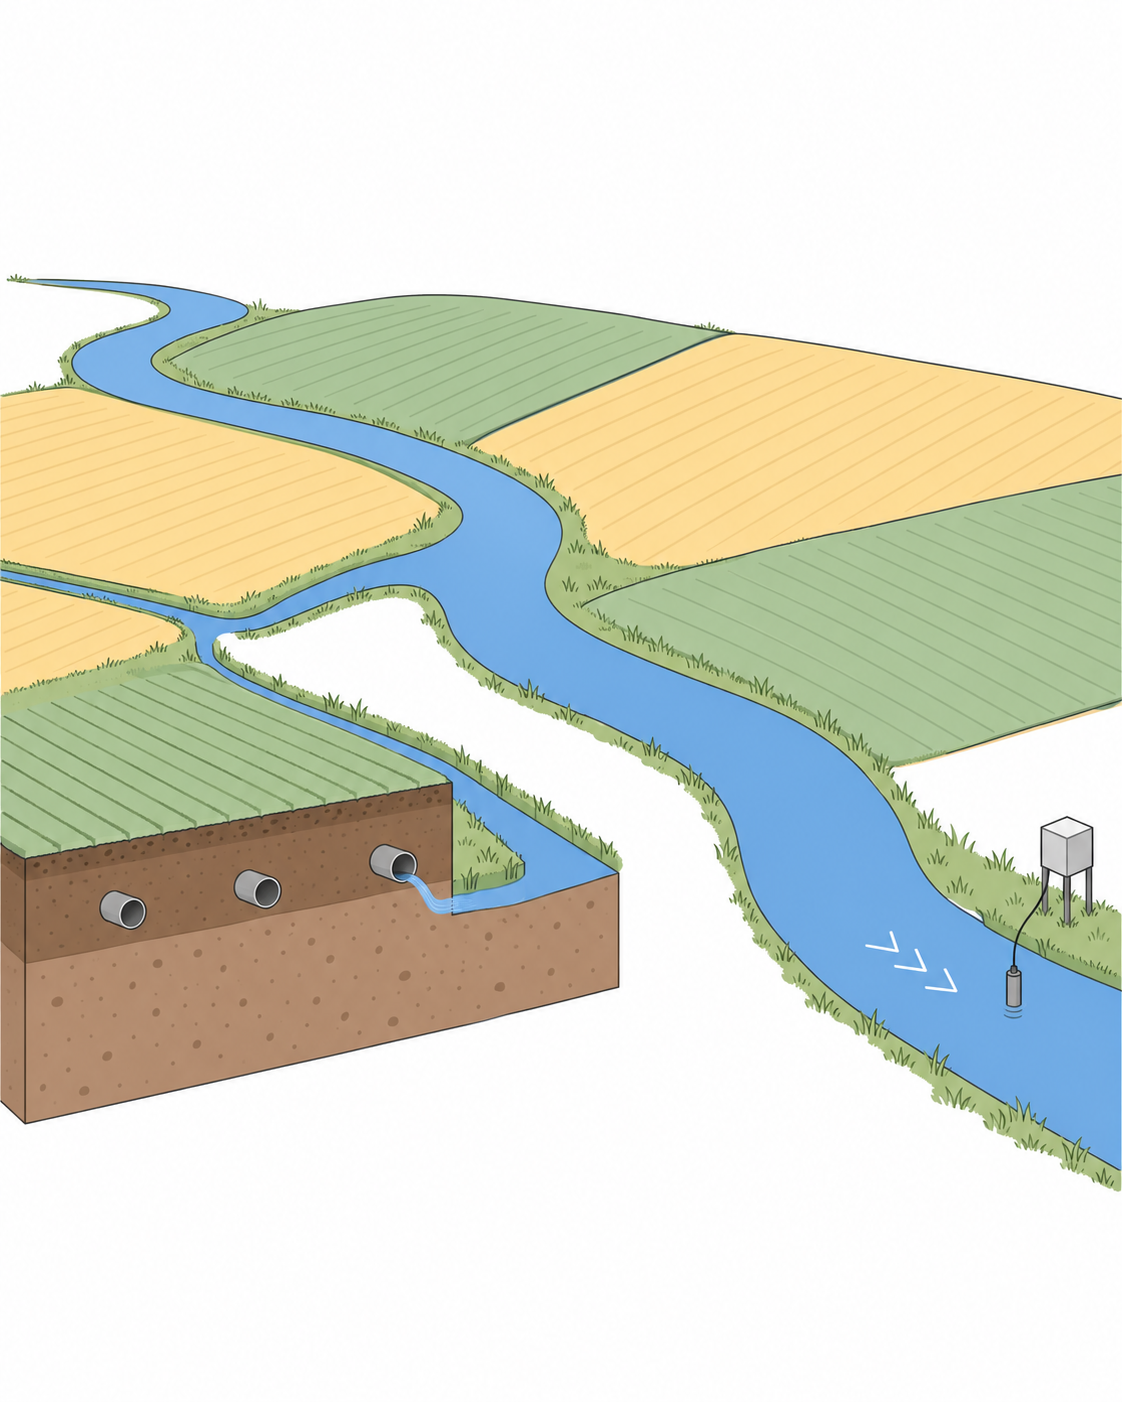
\includegraphics[width=\linewidth]{figures/ch01/ch01-06-site-schematic-brief.png}};
      \begin{scope}[x={(img.south east)},y={(img.north west)}]
        \tikzset{lbl/.style={font=\scriptsize,fill=white,fill opacity=0.8,text opacity=1,inner sep=1pt,align=center}}
        \node[lbl,text width=0.28,align=center] at (0.48,0.86) {农田（玉米—大豆，示意）};
        \node[lbl,text width=0.22,align=center] at (0.20,0.16) {地下排水管};
        \node[lbl,text width=0.18,align=center] at (0.10,0.44) {支沟};
        \node[lbl,text width=0.22,align=center] at (0.52,0.52) {Raccoon River};
        \node[lbl,text width=0.26,align=center] at (0.52,0.10) {监测站 USGS 05484500};
        \node[lbl] at (0.50,0.38) {水流方向};
      \end{scope}
      \end{tikzpicture}
    }{%
      \fbox{\parbox[c][0.36\linewidth][c]{0.34\linewidth}{\centering\scriptsize 缺少 ch01-06 底图\\（codex-image，未在本任务范围）}}
    }
    \par\vspace{1mm}{\scriptsize 示意，不按比例}
  \end{minipage}\hfill
  \begin{minipage}[t]{0.64\linewidth}
    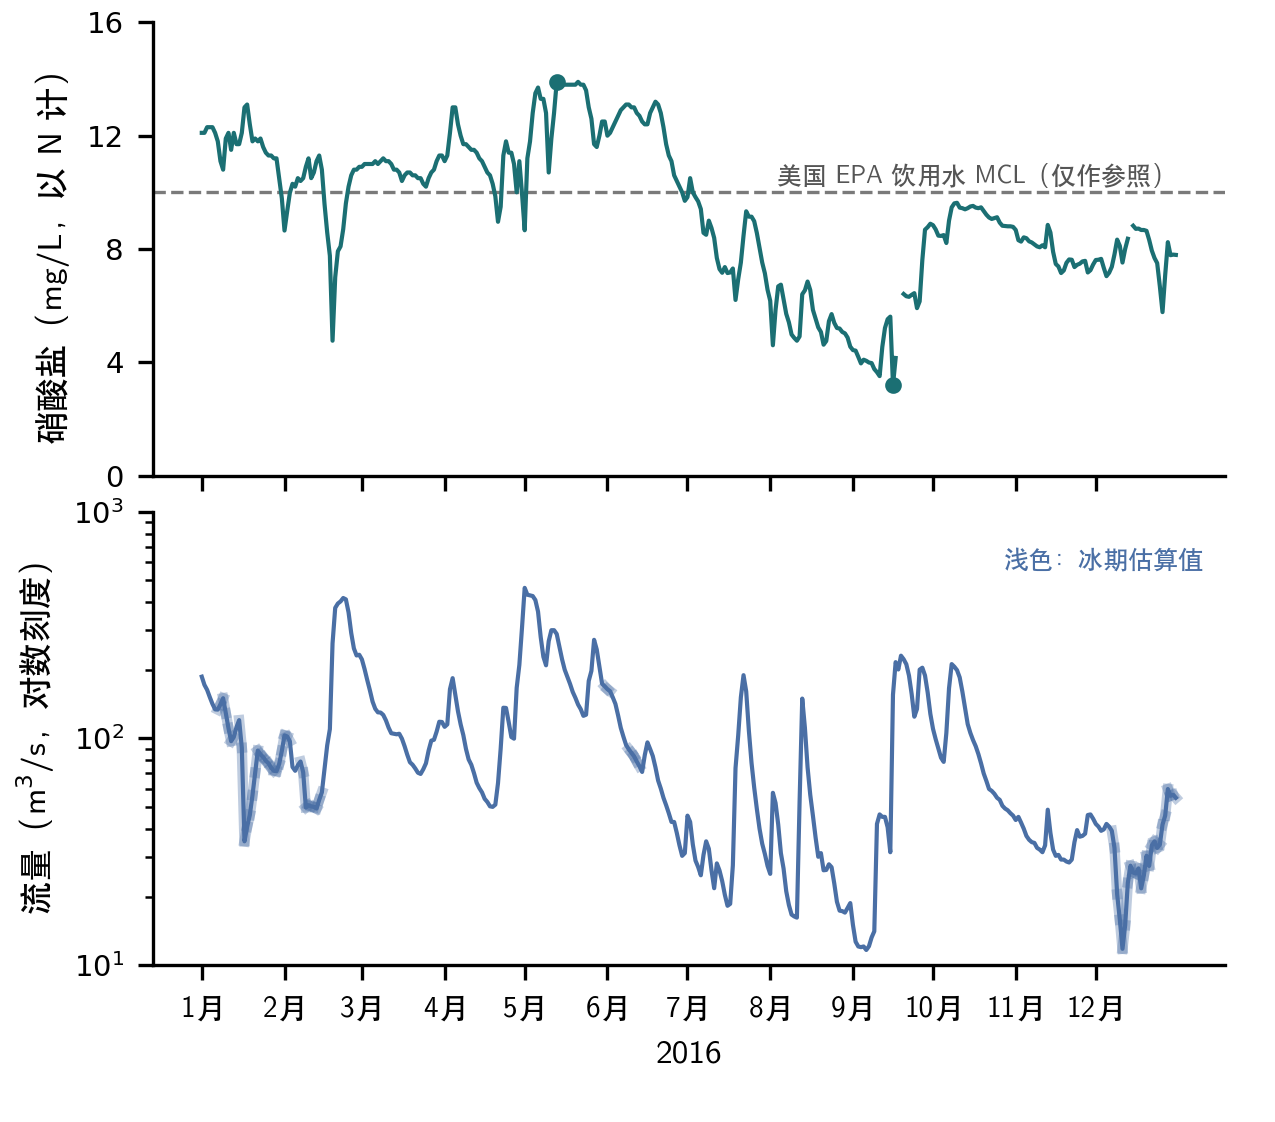
\includegraphics[width=\linewidth]{figures/ch01/ch01-04-nitrate-panel-brief-zh-panel.png}
  \end{minipage}};
\node[anchor=south west,font=\bfseries\small] at ([xshift=1mm,yshift=1mm]panel.north west) {a};
\node[anchor=south west,font=\bfseries\small] at ([xshift=0.34\linewidth,yshift=1mm]panel.north west) {b};
\end{tikzpicture}
}
\caption{\textbf{图 2 示例：2016 年 Raccoon River 的硝酸盐浓度与流量。}（a）研究区简化示意：农田地下排水经支沟汇入河道，下游为 USGS 监测站（05484500，Van Meter, IA）；不按比例，不表示具体地块、管网或污染来源。（b）上：硝酸盐+亚硝酸盐日均浓度（mg/L，以 N 计），缺测日断开；灰色虚线为美国 EPA 饮用水最大污染物浓度 10 mg/L（以 N 计），仅作参照。下：日均流量（$\text{m}^3/\text{s}$，由 $\text{ft}^3/\text{s}$ 换算，对数刻度），浅色段为冰期估算值。数据为 USGS 已审定日均值（公有领域），2026 年 10 月 29 日下载；本图不包含负荷计算或统计检验。示意底图由图像模型生成，标签由作者后期叠加；本章示例图的提示词与生成记录见本书仓库。}\label{fig:ch01-07}
\end{figure}

接着编写图注。若使用图注辅助工具（\sdtool{figure-legend}）上传终稿图起草初稿，作者必须清楚：\textbf{模型只能看到图面像素，不知道站号、下载日期、换算过程和法规适用边界。}作者必须亲手核对并补齐四件事：(1) 站点编号 05484500、地名、已审定状态与下载日期；(2) “以 N 计”单位、缺测断开、$\text{m}^3/\text{s}$ 对数刻度与冰期估算值说明；(3) 声明面板 a“不按比例，不表示具体地块、管网或污染来源”、$10\ \text{mg/L}$ 线“仅作参照”、且“不包含负荷计算或统计检验”（严禁编造样本量或统计量）；(4) 如实说明示意底图由生成工具制作、标签由作者添加。

最后进入第六环节“检查与交付”。先在 $174\ \text{mm}$ 实际印刷宽度下 100\% 缩放检查所有文字（均 $\ge 6\ \text{pt}$）与线条，确保叠加标签未遮挡排水管口或监测站图形；再用图片检查工具（\sdtool{figure-checker}）检测分辨率、色彩空间、灰度对比度与色觉风险。切记\textbf{技术检查通过不等于科学内容正确}，最后必须对照任务书【验收】条款逐项核查全部数据点、断点与图注表述，确认无误后打包归档。

\section{在 SciDraw AI 中选择路线}

打开 \scidraw{} 的“科研绘图向导”（\sdtool{figure-workflow}），先选择要做的图型：\textbf{机制图 / 流程图、数据图、多面板组图、图形摘要}（图~\ref{fig:ch01-08}）。选定后，页面给出一条 3–4 步的有序路线，每一步只有一句说明和一个打开对应工具的按钮。例如“机制图 / 流程图”路线依次为：生成初稿（机制图生成器；画流程图时改用流程图生成器）→ 修改细节（AI 绘图）→ 写图注（图注工具）→ 检查并导出（图片检查）。每一步都可以单独使用，已有初稿可直接从第 2 步开始。

\begin{figure}[htbp]\centering
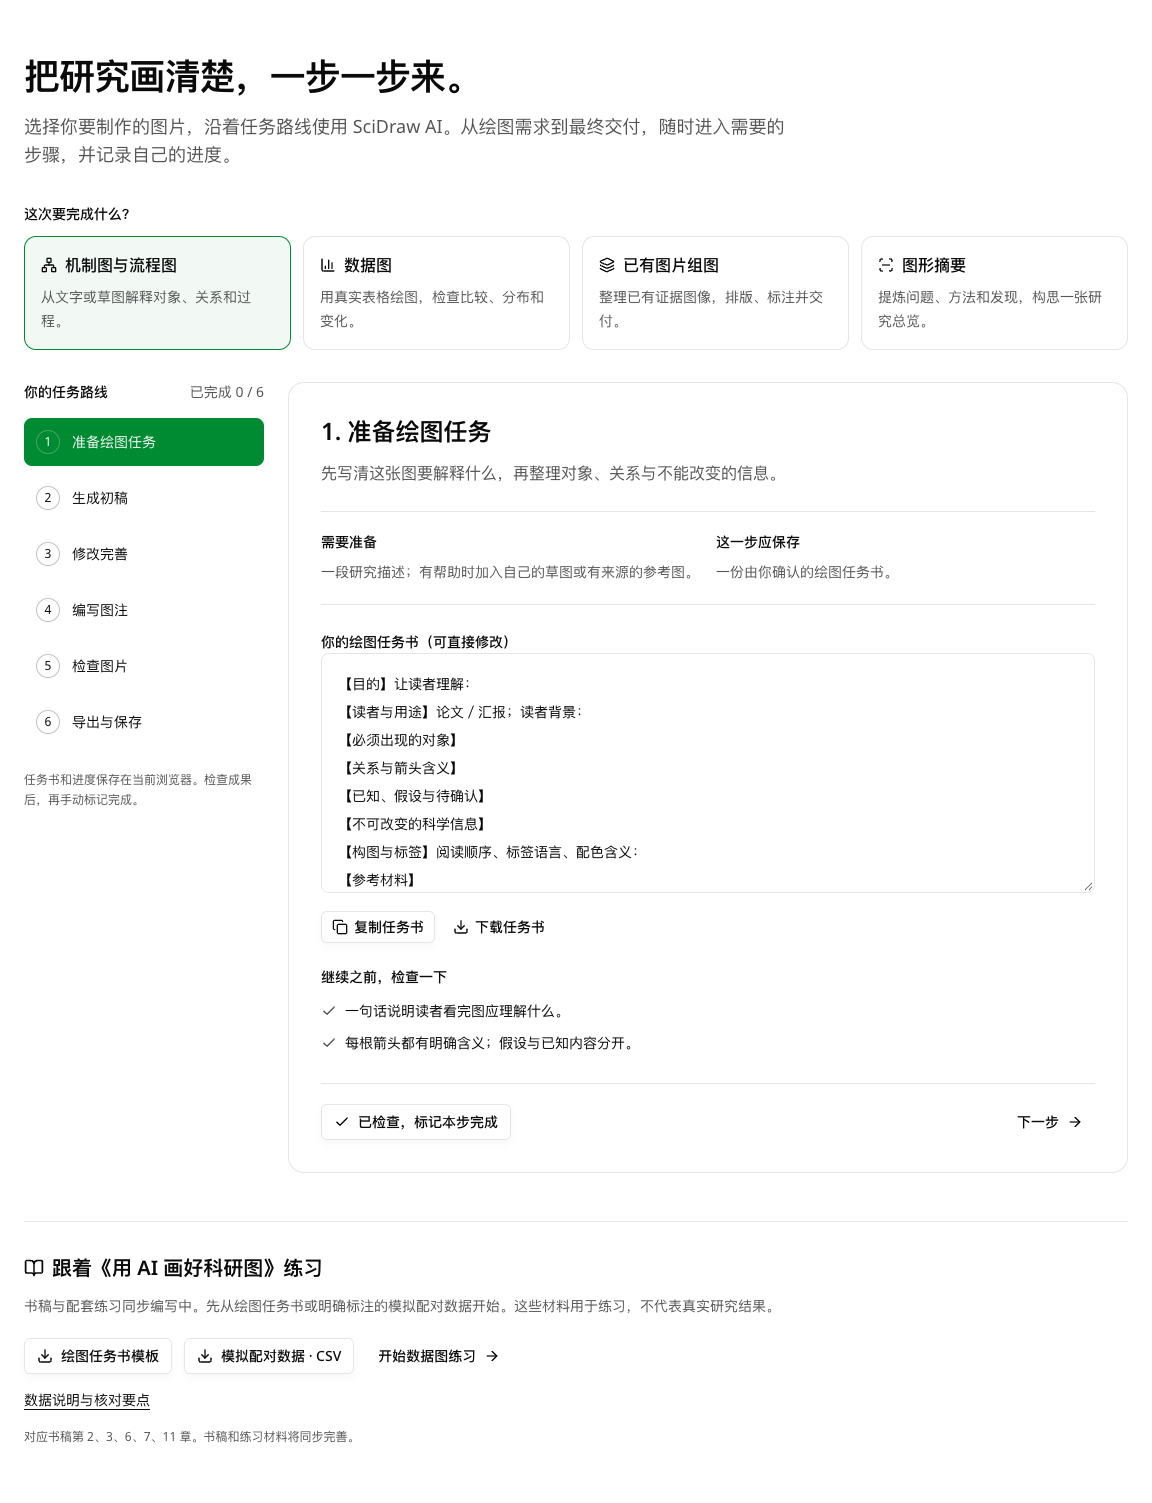
\includegraphics[width=0.92\linewidth,height=0.68\textheight,keepaspectratio]{figures/ch01/ch01-08-guide-ui-zh.png}
\caption{\scidraw{} 科研绘图向导（2026 年 10 月 30 日）。选中“机制图 / 流程图”后，页面列出四步路线——生成初稿、修改细节、写图注、检查并导出，每步附一句说明和打开对应工具的按钮。}\label{fig:ch01-08}
\end{figure}

一张组合图可以串联两条路线：本章案例先走“数据图”路线在科学可视化（\sdtool{sci-vis}）完成面板 b，再走“机制图 / 流程图”路线在流程图或绘图工具（\sdtool{workflow-diagram-generator}、\sdtool{ai-drawing}）完成面板 a，最后进入组图、图注和检查工具。如果你已有现成图片只需补写图注或检查分辨率，也可以直接点进对应步骤。

使用向导时需注意三项平台事实：
\begin{enumerate}
\item \textbf{向导不保存任务书和进度：}页面只给出路线和工具入口，没有任务书编辑框，也不记录你做到了哪一步。任务书写在自己的文档或文本文件里，存进课题文件夹作为记录，进入每一步的工具时粘贴进去。
\item \textbf{跨工具交接采用“下载—上传”：}向导的按钮只负责打开对应工具，不会自动传递任务书或图片；把单面板送往组图、图注或检查工具时，需先下载命名清楚的版本（如 \texttt{panel-b-nitrate-v2.pdf}）再上传，这也能防止误传旧草稿。
\item \textbf{向导不替你做科学审核：}它只给出步骤顺序和工具入口，核实单位、质量码与证据边界仍靠作者自己。
\end{enumerate}

\section{给每张图保留一个小型档案}

在本地硬盘或代码仓库中为每张图建一个结构固定的文件夹，几个月后审稿人要求补图或修改单位时就能随时复现。本章案例的小型档案结构如下：

\begin{Prompt}
fig2-raccoon-nitrate/
  source/   usgs-05484500-2016.rdb（原始下载备份，只读不改）
            raccoon-2016-daily.csv、data-dictionary.md（字段、单位、质量码、DOI、下载日期）
  brief/    figure2-brief-v1.txt（自己保存的任务书）、prompts-log.txt（实际提交的全部输入）
  drafts/   panel-b-draft1.pdf、panel-b-revised.pdf、panel-a-candidates/、
            revision-notes.md（初稿 8 项问题及回退修改记录）
  final/    figure2-final.pdf、figure2-final.tiff、legend-zh.txt、legend-en.txt、
            ai-use.md（使用的功能、日期、输入、采用输出、人工修改）、checks.md
  code/     fetch_usgs.py、plot_nitrate.py
\end{Prompt}

档案不必记录每次鼠标移动，但\textbf{凡是影响科学事实或定量解释的决定都必须留痕}：包括单位换算公式与坐标轴变换、缺测值与质量码的处理规则、示意图剔除无根据元素及从多次生成候选中择优的依据，以及参考线适用范围的界定。同时在 \texttt{ai-use.md} 中如实记录使用的工具功能、日期、实际输入、采用的输出及人工修改；正式投稿前应查阅目标期刊当时的 AI 使用与披露政策。

\section{AI 在这一步能做什么与不能做什么}

六个环节中 AI、确定性工具与作者的职责边界汇总于表~\ref{tab:ch01-01}。

\begin{table}[htbp]\centering\footnotesize
\setlength{\tabcolsep}{3pt}
\renewcommand{\arraystretch}{1.15}
\caption{六个作图环节中 AI 能做什么、不能做什么与作者必须核对的内容。}\label{tab:ch01-01}
\begin{tabularx}{\linewidth}{@{}>{\raggedright\arraybackslash}p{18mm}YYY@{}}
\toprule
\textbf{环节} & \textbf{AI 能做} & \textbf{AI 不能做} & \textbf{作者要核对} \\
\midrule
说明任务 & 根据你的描述起草任务书各栏；指出缺项（如单位、读者、尺寸） & 替你决定图要回答的研究问题；判断结论是否成立 & 目标句是否可检验；用途与尺寸是否真实 \\
准备材料 & 写下载/解析脚本；汇总缺测、质量码；起草数据字典 & 保证数据版本正确；判断“以 N 计”还是“以 $\text{NO}_3^-$ 计”而不读参数说明 & 单位、质量码、下载日期、是否混入临时数据 \\
制作初稿 & 数据图：按明确指令出图；示意图：快速给出构图候选 & 保证不插值、不平滑（除非你写明）；保证示意图不添加未支持的对象 & 逐条对照验收条件；数原始点数；查“多出来的东西” \\
检查并修改 & 执行具体修改指令；按问题表重出图 & 判断修改是否引入新错误；只改一处而不动其他部分（图像修改可能影响整张图） & 每次修改后重新全量核验，包括没要求改的部分 \\
组织说明 & 组图排版、编号、尺寸预设；起草图注 & 知道站号、下载日期、处理方式等图中看不见的信息；编造样本量和统计量是禁止的 & 图注每个数字与说明是否有出处 \\
检查与交付 & 技术检查（分辨率、色彩、灰度、色觉风险） & 科学审核；替你确认期刊 AI 政策 & 终尺寸可读性；交付包能否让他人复现 \\
\bottomrule
\end{tabularx}
\end{table}

\section{本章检查清单}

\begin{itemize}
\item 我能用一句话写出这张图的目标，并且它能决定图型、布局或标签。
\item 我已判断每个面板的材料类别，数据面板走确定性绘图，示意面板不画未经支持的对象。
\item 原始数据保留未改动的副本；单位、质量码、缺测与下载日期写进了数据说明。
\item 实际提交给工具的每段输入都保存了下来。
\item 每一版修改都有记录：改了什么、为什么、回到了哪个环节。
\item 终稿在实际使用尺寸下检查过文字和线条。
\item 图注中的每个数字、来源、处理方式都能在档案中找到依据。
\item 每一步的输出都是我对照任务书核对后才进入下一步的，而不是打开过工具页面就算完成。
\item 交付包里有 AI 使用记录；投稿前查过目标期刊当时的要求。
\end{itemize}

\section{练习}

\begin{enumerate}
\item \textbf{（目标句）}为本章案例另写两个不同的目标句：一个关注“春季高浓度持续多少天”，一个关注“低流量期的浓度”。分别说明它们会让图型、时间范围或标注怎样变化。
\item \textbf{（找错）}不看第 1.4 节修改单，列出图~\ref{fig:ch01-03} 与图~\ref{fig:ch01-05} 中至少 5 个问题，并为每个问题写一句可以核对的修改指令；再判断每个问题应回到六个环节中的哪一个。
\item \textbf{（\scidraw{} 实操）}从 USGS 下载另一个有硝酸盐传感器的站点（或你自己研究中的一份时间序列）的一年日均值，按第 1.4 节格式把任务书写在自己的文档里，再在科研绘图向导（\sdtool{figure-workflow}）选“数据图”，从第 1 步进入 \sdtool{sci-vis} 上传数据、粘贴任务书中的绘图要求，生成后对照验收条件逐条打勾，记录至少一次修改指令及其效果。把整个过程按第 1.6 节结构存档。
\end{enumerate}

\section*{参考文献}

\begin{itemize}
\item Pellerin BA, Stauffer BA, Young DA, Sullivan DJ, Bricker SB, Walbridge MR, Clyde GA, Shaw DM. Emerging tools for continuous nutrient monitoring networks: sensors advancing science and water resources protection. \textit{JAWRA Journal of the American Water Resources Association}. 2016;52(4):993--1008. doi:10.1111/1752-1688.12386
\item Rougier NP, Droettboom M, Bourne PE. Ten simple rules for better figures. \textit{PLoS Computational Biology}. 2014;10(9):e1003833. doi:10.1371/journal.pcbi.1003833
\item Schilling K, Zhang Y-K. Baseflow contribution to nitrate-nitrogen export from a large, agricultural watershed, USA. \textit{Journal of Hydrology}. 2004;295(1--4):305--316. doi:10.1016/j.jhydrol.2004.03.010
\item U.S. Environmental Protection Agency. National Primary Drinking Water Regulations (nitrate MCL 10 mg/L as N). \url{https://www.epa.gov/ground-water-and-drinking-water/national-primary-drinking-water-regulations}
\item U.S. Geological Survey. USGS water data for the Nation: National Water Information System database, site 05484500. \url{https://doi.org/10.5066/F7P55KJN} (accessed 2026-10-29).
\item Weissgerber TL, Milic NM, Winham SJ, Garovic VD. Beyond bar and line graphs: time for a new data presentation paradigm. \textit{PLOS Biology}. 2015;13(4):e1002128. doi:10.1371/journal.pbio.1002128
\end{itemize}

\chapter{把研究内容变成一份绘图任务书}


研究者往往能够用几分钟向同事讲清一个课题，却难以用几句话告诉绘图工具应该画什么。口头交流允许随时补充前提，也能借助双方共有的背景。绘图输入则需要把这些隐含内容写出来。

例如，“画一张通路图，体现上游激活、下游作用以及抑制剂干预”，听起来已经像一个完整任务。但上游是谁？激活的是哪个对象？下游作用是观测结果还是推测？抑制剂影响哪个环节？这些问题没有答案时，生成图片只能自行填充结构。

绘图任务书的作用，是把作者掌握的研究内容变成一份可以执行和检查的说明。

\section{任务书与提示词各管什么}

任务书记录你希望表达的内容及其依据。提示词则针对一次操作，把任务书中的相关部分交给工具。它们可以非常接近，也可能随着操作阶段不同而有明显差别。

初次生成需要解释对象、关系和布局。调整颜色时，可能只需要给出新的颜色分工及保持不变的内容。补写图注时，则需要图和相应的文字说明。任务书帮助你判断这些局部操作是否仍然服务于同一个目标。

因此，不必为了写出一个“万能提示词”把所有要求塞进一段长文字。先把任务书写清，再为具体步骤选取信息。后续修改涉及科学内容时，也应更新任务书，避免旧版本的说明继续驱动新图。

\section{用七个问题构成任务书}

配套模板有十个填写项。实际思考时，可以用下面七个问题组织它们。

\textbf{第一，给谁看，在哪里用？} 同一研究可以为领域同行、跨学科评审或课堂读者制作不同图片。用途还决定了最终观看尺寸。写“论文结果部分，供了解基本方法的同行阅读”，比只写“论文风格”更能影响取舍。

\textbf{第二，主要回答什么问题？} 用一句话写出图的中心任务。如果句子里连续出现多个“以及”，试着把它拆成几个面板，并为每个面板分配一个问题。

\textbf{第三，依据哪些材料？} 记录文件名、工作表、实验记录或文献位置。材料不是越多越好，而是要能够支持这张图里的每个重要陈述。不同版本的结果不要混在同一个输入中。

\textbf{第四，必须出现哪些对象和关系？} 列出对象后，还要说明它们的对应关系、方向、分组与空间位置。数据图中的“同一对象两次测量”也是关系，需要与机制图中的箭头一样明确。

\textbf{第五，哪些是事实，哪些是解释？} 观测、推断和假设需要保持各自的身份。任务书中写明不确定性，图中再用标签或约定线型表达，并在图例中解释。不能把一条没有证据的关系交给工具自行决定。

\textbf{第六，希望怎样呈现？} 此时再确定图型、阅读方向、面板、颜色角色和标签语言。给出能帮助理解内容的约束，避免用大量形容词代替具体布局。

\textbf{第七，怎样知道完成了？} 列出可核对的条件，如对象数量正确、箭头逐条对应、所有原始数值保留、文字在最终尺寸可读。验收条件应与实际输入和研究材料连接起来。

如果某一项尚不清楚，写“待确认”。这既为你留下下一步任务，也避免让漂亮的初稿提前替你做决定。

\section{把名词清单改成关系表}

下面使用一个完全抽象的教学模型。设 R、K、P 和 I 是四个符号。为了练习，我们人为规定：R 对 K 有激活作用；K 与 P 之间存在一条假设的影响关系；I 抑制 K。它们不代表任何真实生物学机制。

如果只输入“R、K、P、I，机制图，蓝绿色，简洁”，得到什么样的连接都难以事先判断。把它改成关系表后，要求就具体了。

\begin{center}\small
\begin{tabularx}{\linewidth}{YYYYY}
\toprule
\textbf{起点} & \textbf{终点} & \textbf{本例规定的含义} & \textbf{表达方式} & \textbf{验收依据} \\
\midrule
R & K & 教学模型给定的激活关系 & 实线箭头，旁标“激活” & 方向为 R \ensuremath{\rightarrow} K \\
K & P & 尚待验证的影响关系 & 虚线箭头，旁标“假设” & 与实线明确区分 \\
I & K & 教学模型给定的抑制关系 & 末端短横线，旁标“抑制” & 不画成激活箭头 \\
\bottomrule
\end{tabularx}
\end{center}

\begin{figure}[htbp]\centering
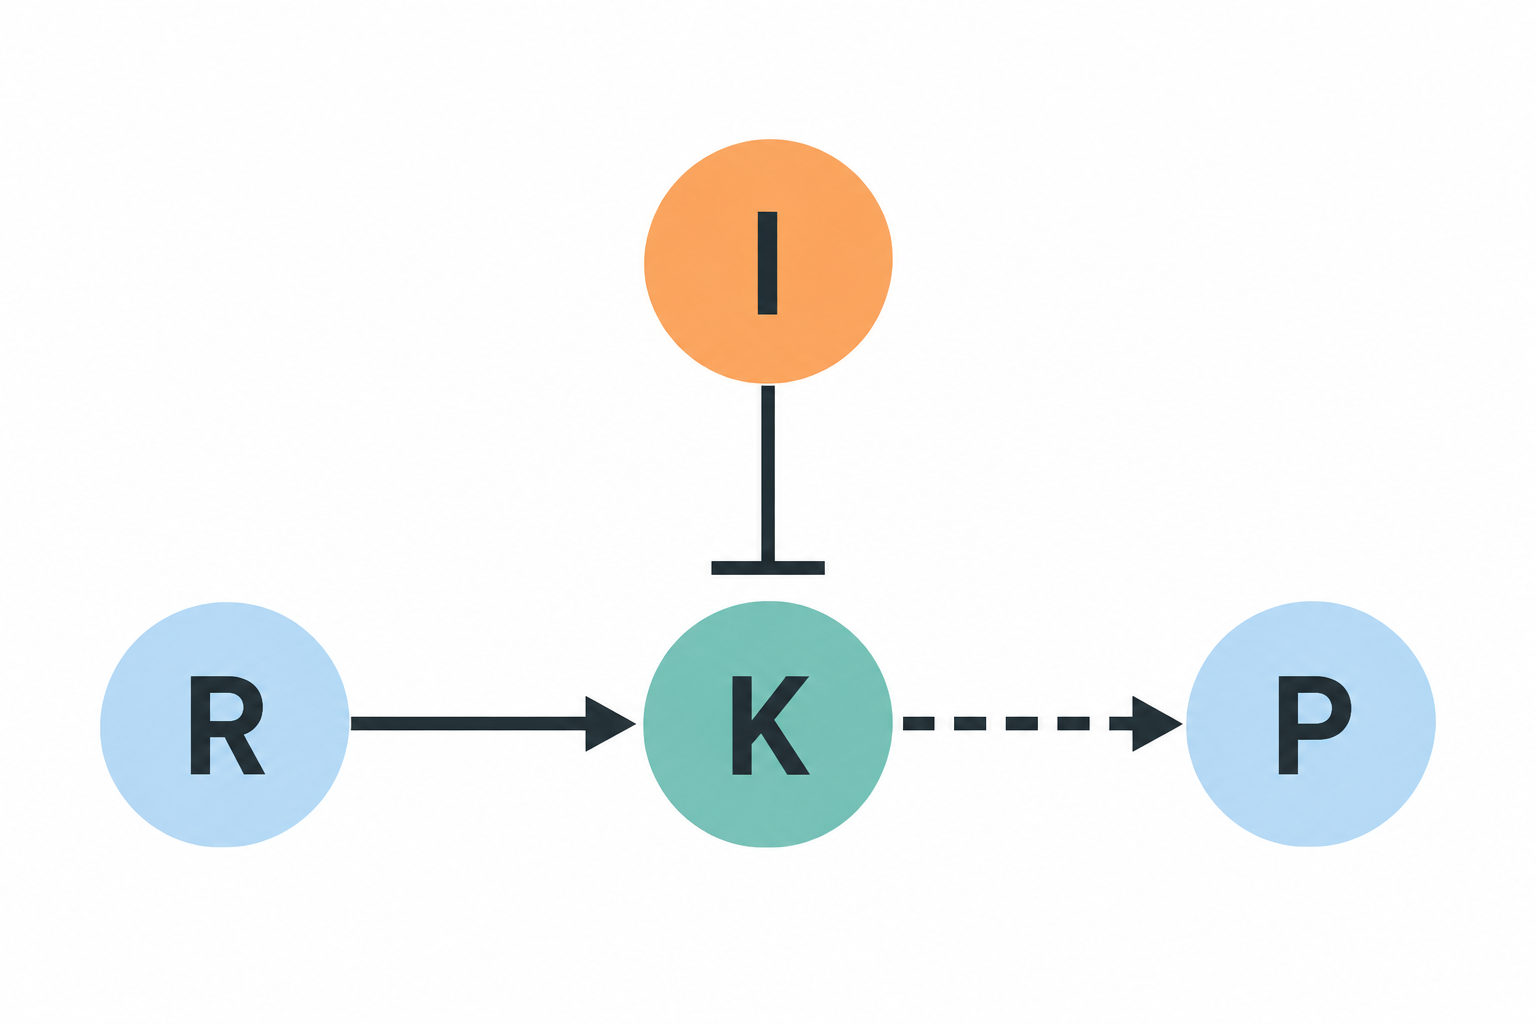
\includegraphics[width=\linewidth]{figures/mechanism-codex.png}
\caption{Codex 内置图像生成的抽象教学模型。实线箭头表示给定的激活关系，虚线箭头表示假设关系，T 形终点表示抑制。四个符号与全部关系均为教学设定，不对应真实分子或研究发现。}\label{fig:mechanism}
\end{figure}


线型和箭头没有脱离语境的万能含义。它们的意义由学科惯例、本图定义和图例共同确定。本例使用上述约定，是为了让读者区分三种关系。真实项目应采用目标学科能理解的表达，并在可能产生歧义时直接标注。

用关系表检查图时，可以逐行进行：找 R 和 K，检查方向，再找标签。之后检查 K 到 P 的线是否仍为虚线，最后确认 I 的抑制终点确实是 K。检查任务从“这图看起来对吗”变成了几个可定位的问题。

\section{为机制案例写一份可执行的输入}

在 SciDraw AI 科研绘图向导中选择“机制图与流程图”，把默认任务书替换为下面的内容，并下载一份副本。

\begin{Prompt}
【用途与读者】用于科研绘图教学，读者无需生物学背景。
【目标】让读者分辨给定关系、假设关系和抑制关系。
【材料】仅使用本任务书的抽象教学设定。
【对象】R、K、P、I；每个对象各出现一次。
【关系】
R 激活 K：实线箭头，方向 R 到 K，旁标“激活”。
K 可能影响 P：虚线箭头，方向 K 到 P，旁标“假设”。
I 抑制 K：线条终点在 K 一侧使用短横线，旁标“抑制”。
【布局】R、K、P 从左到右；I 放在 K 上方。
【视觉】白底、二维简洁图形。四个对象以标签识别。
【限制】不添加其他对象、关系、分子形态或实验结果。
【图例】解释实线、虚线与抑制线；标注“抽象教学模型”。
【验收】四个对象、三条关系、方向与标签逐项对应。
\end{Prompt}

这个输入没有要求“达到某顶级期刊水平”。它给出了更直接的质量标准：对象可辨，关系准确，假设没有被画成确定结论。颜色可以随后调整，基本关系要先站得住。

进入机制图工具后，复制这段说明到生成输入。得到候选图时，先按关系表检查，再决定是否继续修改。如果输出多了一个对象，不能只要求“整体更简洁”；应指出多出的对象，以及保留四个对象各一次的要求。

本版已用 Codex 内置图像生成制作了图 2-1，记录了完整输入与核验结果。四个对象和三条关系均符合任务书，节点仍有轻微渐变，因此它是可核对的教学候选图，不是“所有风格要求都已精确执行”的证明。该图并非 SciDraw AI 实测输出。AI 的每一次输出都具有变动性，同一段输入并不保证自动满足全部条件。

\section{为数据图写约束，要具体到列}

数据图的任务书需要从研究设计延伸到数据结构。第一章的练习只有三列，也足以说明几种常见歧义。

\texttt{sample\_id} 用来识别同一个对象；\texttt{before} 和 \texttt{after} 是该对象的两次测量。八行对应八个虚构对象，同时包含十六个观测值。对象数和测量数应分别表述。对真实研究，还需解释实验单位、重复测量和技术重复之间的关系。

下面是一段适合交给科学可视化的绘图要求：

\begin{Prompt}
读取上传的 paired-example.csv。
sample_id 是配对键；before 和 after 是两次测量，单位 a.u.。
绘制配对点线图：横轴按 before、after 排列，每个对象的两个点
由一条线相连。保留全部八个对象和原始十六个观测值。
不要把两列当成互不相关的独立样本，也不要连接不同对象。
标题为“模拟教学数据：个体前后变化”。
本练习只展示原始测量，不进行显著性检验，不添加误差线。
不得删去 SIM04 或把它的下降趋势改成上升。
\end{Prompt}

最后一句不是要求某个真实研究必须出现下降，而是本练习的核查点：文件里这个对象确实从 18 下降到 17。真实项目应依据自己的数据写核查点，不能用期望的结论倒逼图形。

输入中“不添加误差线”也只针对本次练习。其他图需要误差线时，应明确它表示标准差、标准误、置信区间或其他量，并说明计算依据。AI 无法仅凭“加上常见误差线”知道你希望传达哪种不确定性。

\section{使用 PDF 辅助时，先确认读取了什么}

论文中的信息分散在摘要、正文、图表、补充材料和方法里。上传一个 PDF 后，系统如何提取文字，会直接影响后续提示词包含哪些内容。

本次核查的 SciDraw AI PDF 辅助路径读取前五页，并从摘要或开头截取有限文本，供视觉提示词使用。它适合帮助起草研究总览，但不能据此认定整篇论文、所有图表与补充材料都已经被理解。

使用这一入口时，可先准备一份作者确认的要点：研究问题是什么，采用了哪条主要方法，准备展示哪个结果，还有哪些适用条件。将辅助生成的提示词与这份要点对照，补回遗漏，再进入绘图。若关键结果只在后文，单凭前几页输入就可能遗漏它。

在任务书来源栏记录读取范围也很有用。例如：“输入为作者整理的摘要与结果要点；PDF 辅助仅用于初稿，关键结论已对照原文确认。”这比笼统写“根据全文自动生成”准确，也便于以后重新制作。

\section{把模糊意见改写成可核对的请求}

很多重复生成并没有明确方向，只是在等待一个更合眼缘的结果。下面几种改写，可以让一次操作承担清楚的任务。

\begin{center}\small
\begin{tabularx}{\linewidth}{YY}
\toprule
\textbf{模糊表达} & \textbf{更具体的请求} \\
\midrule
画得更专业 & 将 R、K、P 水平对齐；统一标签字号；保留关系和对象数量 \\
更突出结果 & 让读者能直接比较两次测量；保留个体连线与全部观测值 \\
简化一点 & 移除装饰背景和重复说明，保留四个对象、三条关系与图例 \\
用期刊风格 & 白底，减少装饰；按已确认的文字层级与颜色角色重新排版 \\
自动补全图注 & 起草可从图中识别的描述；样本量、实验条件与统计方法由作者补充 \\
\bottomrule
\end{tabularx}
\end{center}

这些写法不保证模型绝不出错。它们的价值在于让作者能够判断要求是否执行，并定位需要重做的部分。平台当前的图片修改可能影响整张图，所以即使只要求改一个标签，也要重新检查其他对象和关系。

\section{在提交前，做一次反向阅读}

把任务书当作你第一次看到的材料，暂时不依赖脑中的研究背景，逐句寻找不完整的地方。

“处理组高于对照组”缺少哪个指标、什么条件和哪些证据。“这个步骤之后分成两组”缺少分组依据。“提高性能”缺少指标、单位和比较对象。发现这种缺口后，先补充信息，或把结论降为待确认事项。

还可以为每条拟表达的陈述建立一个小表：陈述、来源位置、拟采用的图形、需要确认的内容。真实项目中的来源可以具体到数据列、文件版本或记录页码。抽象练习则标注“教学设定”。这样做能避免来源模糊的陈述被顺手写进图中。

\section{本章练习与验收}

完成两份任务书：一份针对自己的研究，另一份使用本章抽象机制或配对数据。保留一份修改前的原始说明，再写一段修改记录，说明你补充了哪些关系、来源和验收条件。

最后逐项检查：对象能否数清，关系能否逐条核对，数据约束能否对应到列，未知信息是否仍被明确标识，最终产物是否有具体用途。

完成这些工作后，你就拥有了一个可以进入绘图阶段的输入。第三章将讨论如何把同一份任务书展开成不同构图，并用读者的理解成本来选择方案。

\chapter{与 AI 一起推演构图和草图}
\usetikzlibrary{decorations.pathreplacing}

分子生物学博士生林悦正在准备学位论文开题报告，同时为一篇基因组编辑综述撰写引言。她需要制作全篇的第一张总览图（Figure 1），向跨细分方向的生命科学同行与评审交代化脓链球菌 Cas9（SpCas9）如何在单链引导 RNA（sgRNA）引导下识别原间隔序列邻近基序（PAM）并切开双链 DNA，以及非同源末端连接（NHEJ）与同源定向修复（HDR）两条主要修复途径如何决定不同的编辑结局。

她打开图像生成工具，输入了一句看似省事的指令：“画一张专业、有视觉冲击力的 CRISPR–Cas9 基因编辑机制总览图，适合顶刊发表。”几十秒后，工具生成了一张色彩饱满的横版插图：深蓝色的立体细胞核背景中央悬着一把发着青光的剪刀，正在剪断一条扭曲的三维双螺旋 DNA；画面的四个角落散落着一段飘带状的 RNA、一枚标着“PAM”的发光徽章，以及两段分别带有裂痕和彩色补丁的短双链。

林悦觉得画面的光影质感远超自己用基础绘图软件拼出的线框，便直接放进了开题幻灯片。没想到导师看了一眼屏幕，只用了五秒钟就问出一句话：“这张图应该从哪里开始看？”

林悦一时语塞。导师接着指着屏幕追问：读者的第一眼会被正中央最大的发光剪刀吸引过去，可切割双链明明是第三步；看完剪刀之后，视线该往左上角找 RNA，还是往右下角看修复结果？左下角和右下角的两段 DNA 之间既没有连线也没有基线对齐，读者怎么知道它们是由同一个断裂分出来的两条并列修复途径，而不是一前一后的两个步骤？

这张初稿的问题不在画功，而在于作者点击“生成”按钮之前，没有替读者决定视线的落脚点与行进路线。只要输入中缺少明确的构图骨架，模型就会按照装饰画的对称习惯把元素随机摊在画布上，让读者的视线在四个角落之间来回乱撞。本章把构图推演与草图设计提前到精细渲染之前，依次解决五个问题：如何用“入口—路径—终点”控制阅读顺序，如何判断哪些内容应该放进同一个面板，如何针对同一份任务书画出三种结构不同的草图骨架，如何在 \scidraw{} 中由草图生成候选图并按写明的标准做出选择，以及如何用“每次只改一个可核对目标”的纪律完成定稿。

\section{读者的视线先于画面}

审稿人或读者翻开论文看到一张总览图时，并不是像读正文那样逐字扫描，而是在最初几秒钟内先靠视觉本能寻找落脚点，再顺着画面提供的几何线索往下走（Wong，2011c；Rougier 等，2014）。如果一张图不能在前五秒内让读者看懂“从哪开始、往哪走、最后停在哪”，里面的分子局部画得再精致，也会在读图时制造理解阻力。

在动笔或输入提示词之前，作者应当先用三个问题替读者规划好视线轨迹：

\begin{itemize}
\item \textbf{第一，入口在哪里？} 读者的第一眼必然落在画面中视觉权重最大的地方——通常是面积最大、明度或色彩对比最高、造型最孤立，或者位于日常阅读习惯起点（横排出版物为左上角或左端）的元素。如果一张图没有安排明确的入口，或者同时摆放了三四个尺寸相当、对比度都很强烈的团块，读者在进入画面的瞬间就会陷入犹豫。
\item \textbf{第二，路径怎么走？} 进入画面之后，视线需要明确的几何向导。最直接的向导是单向箭头和步骤编号（1、2、3……）；更底层也更稳定的向导则是元素的水平与垂直对齐基线、连续留白形成的通道，以及顺应阅读习惯的推进方向（从左到右、从上到下）。
\item \textbf{第三，终点停在哪里？} 视线走完路径停驻的位置，应当恰好承载这张图最核心的科学结论。在包含因果或时间链条的总览图中，如果把上游的常见背景组件画得硕大无比，而把真正需要读者比对的实验结局或修复结果挤在角落里，就会造成头重脚轻，让主要信息沦为视觉附庸。
\end{itemize}

\begin{figure}[htbp]\centering
\resizebox{\linewidth}{!}{% FIG ch03-01 reading order (Chinese)
\begin{tikzpicture}[
  x=1mm, y=1mm,
  font=\sffamily\footnotesize,
  panel/.style={draw=BookInk!40, line width=0.3pt, rounded corners=1pt},
  block/.style={
    rounded corners=2pt, draw=black!60, fill=black!5,
    minimum size=7mm, inner sep=0pt, font=\sffamily\footnotesize,
  },
  eye/.style={line width=4pt, draw=blue!50, opacity=0.35, rounded corners=2pt},
  paneltitle/.style={font=\sffamily\scriptsize, text=BookInk, align=center},
]
  \def\pw{50}\def\ph{35}
  \begin{scope}[shift={(0,42)}]
    \draw[panel] (0,0) rectangle (\pw,\ph);
    \node[paneltitle, anchor=north] at (0.5*\pw,\ph+2.5) {(a) 线性};
  \end{scope}
  \begin{scope}[shift={(54,42)}]
    \draw[panel] (0,0) rectangle (\pw,\ph);
    \node[paneltitle, anchor=north] at (0.5*\pw,\ph+2.5) {(b) 中心辐射};
  \end{scope}
  \begin{scope}[shift={(108,42)}]
    \draw[panel] (0,0) rectangle (\pw,\ph);
    \node[paneltitle, anchor=north] at (0.5*\pw,\ph+2.5) {(c) 两分支};
  \end{scope}
  % (a) linear 1-5
  \begin{scope}[shift={(0,42)}]
    \foreach \i/\x in {1/8,2/18,3/28,4/38,5/42} {
      \node[block] at (\x,17.5) {\i};
    }
    \draw[eye] (6,22) .. controls (15,26) and (35,26) .. (44,22);
    \foreach \i/\xa/\xb in {1/11/15,2/21/25,3/31/35,4/41/45} {
      \draw[-{Stealth[length=1.2mm]}, draw=BookInk!35, thin] (\xa,17.5) -- (\xb,17.5);
    }
  \end{scope}
  % (b) hub
  \begin{scope}[shift={(54,42)}]
    \node[block] at (25,17.5) {3};
    \node[block, minimum size=5.5mm] at (8,28) {1};
    \node[block, minimum size=5.5mm] at (42,28) {2};
    \node[block, minimum size=5.5mm] at (8,7) {4};
    \node[block, minimum size=5.5mm] at (42,7) {5};
    \draw[eye, blue!50] (25,20) .. controls (32,26) .. (42,28);
    \draw[eye, orange!70!black, opacity=0.35] (25,20) .. controls (18,26) .. (8,28);
    \draw[eye, blue!50] (25,15) .. controls (32,8) .. (42,7);
    \node[font=\Large, text=BookInk!60] at (32,17) {?};
  \end{scope}
  % (c) two-branch
  \begin{scope}[shift={(108,42)}]
    \foreach \i/\x in {1/10,2/25,3/40} {
      \node[block, minimum size=6mm] at (\x,28) {\i};
    }
    \node[block, minimum size=6mm] at (25,12) {4};
    \node[block, minimum size=6mm] at (25,5) {5};
    \draw[-{Stealth[length=1mm]}, draw=BookInk!35, thin] (13,28) -- (22,28);
    \draw[-{Stealth[length=1mm]}, draw=BookInk!35, thin] (28,28) -- (37,28);
    \draw[-{Stealth[length=1mm]}, draw=BookInk!35, thin] (40,26) -- (40,20) -- (25,20) -- (25,15);
    \draw[-{Stealth[length=1mm]}, draw=BookInk!35, thin] (25,20) -- (25,8);
    \draw[eye] (8,30) .. controls (18,32) .. (38,30) .. controls (42,22) .. (25,14);
    \draw[eye] (25,14) -- (25,6);
  \end{scope}
  % bottom row: proximity, alignment, enclosure, hierarchy
  \def\bw{38}\def\bh{22}
  \foreach \i/\x/\title in {
    1/0/接近, 2/42/对齐, 3/84/围合, 4/126/主次} {
    \begin{scope}[shift={(\x,0)}]
      \draw[panel] (0,0) rectangle (\bw,\bh);
      \node[paneltitle, anchor=north] at (0.5*\bw,-2.5) {\title};
    \end{scope}
  }
  \begin{scope}[shift={(0,0)}]
    \foreach \x in {6,10,14} {\fill[BookInk] (\x,14) circle (0.9mm);}
    \foreach \x in {26,30,34} {\fill[BookInk] (\x,14) circle (0.9mm);}
  \end{scope}
  \begin{scope}[shift={(42,0)}]
    \draw[fill=BookInk!15, draw=BookInk!50] (4,6) rectangle (16,18);
    \draw[fill=BookInk!15, draw=BookInk!50] (4,6) rectangle (14,18);
    \node[font=\scriptsize, anchor=west] at (18,12) {对齐};
    \node[font=\scriptsize, anchor=west, text=BookInk!55] at (18,7) {不对齐};
  \end{scope}
  \begin{scope}[shift={(84,0)}]
    \draw[fill=BookRule!40, rounded corners=2pt] (3,5) rectangle (35,19);
    \foreach \x in {10,19,28} {
      \draw[fill=BookPale, draw=BookInk!40, rounded corners=1pt] (\x-3,9) rectangle (\x+3,15);
    }
  \end{scope}
  \begin{scope}[shift={(126,0)}]
    \draw[fill=BookInk!25, draw=BookInk!60, rounded corners=2pt] (14,6) rectangle (26,18);
    \foreach \x/\y in {6/16,6/10,32/16,32/10} {
      \draw[fill=BookInk!8, draw=BookInk!45, rounded corners=1pt] (\x-2.5,\y-2) rectangle (\x+2.5,\y+2);
    }
  \end{scope}
\end{tikzpicture}
}
\caption{阅读顺序由布局决定。上：同样五个元素按三种结构排列，半透明曲线表示读者最可能的视线路径；中心辐射式没有唯一入口，读者可能沿不同路径阅读。下：控制主次与分组的四种基本手段。}\label{fig:ch03-01}
\end{figure}

图~\ref{fig:ch03-01} 上排展示了同样五个事件节点（编号 1 至 5）在三种不同布局结构下的视线走向。在图~\ref{fig:ch03-01}a 的\textbf{线性布局}中，五个圆角方块从左到右排成一行，由灰色细箭头相连；半透明蓝色粗曲线标出了毫无歧义的视线路径——从左端节点 1 进入，顺着箭头一路向右，在右端节点 5 结束。这种结构天然契合单一时间序列或单向实验流程。

再看图~\ref{fig:ch03-01}b 的\textbf{中心辐射布局}。节点 3 被放在画布正中央且尺寸较大，节点 1、2、4、5 分散在四个角落。这种排法在头脑风暴或概念关联图中很常见，但一旦用于表达有先后顺序的科学过程，就会立刻制造阅读障碍：图中叠加的蓝色与橙色两条半透明曲线表明，不同读者会走出截然不同的路径——有人先被正中央的节点 3 吸引，随后随机跳向右上角的 2 或右下角的 5；有人习惯性地先看左上角的 1，经过中央的 3 之后却不知道下一步该去右上角还是左下角。中央旁边的问号标出了这种决策困惑：当画面缺乏唯一入口且四周节点地位均等时，读者只能靠猜来拼凑事件顺序。

图~\ref{fig:ch03-01}c 则展示了适合表达“共同上游、两种结局”的\textbf{两分支布局}。节点 1、2、3 在上排从左到右紧凑排列，交代共同前提步骤；从节点 3 向下引出分叉箭头，接入下方上下并列的节点 4 与节点 5。读者的视线先沿上排完成水平扫描，随后顺着分叉箭头向下进入并列对比区，既不会弄混上游与下游的先后次序，又能直观看出 4 和 5 是由同一个节点 3 分化出来的两条平行支路。

看清了骨架对路径的控制作用，下一步是掌握调控画面内部秩序的四项基本视觉手段（图~\ref{fig:ch03-01} 下排）。前三项直接源自格式塔（Gestalt）视觉感知原则（Wong，2010a，2010b），第四项则是构建视觉层级的核心法则（Wong，2011d）：

\begin{enumerate}
\item \textbf{接近（Proximity）：} 空间距离相近的元素会被大脑自动归为同一组。如图~\ref{fig:ch03-01} 下排左一所示，六个完全相同的圆点不需要任何边框，仅靠“组内间距小、组间间距大”就自然分成了左右两群。在科研图中，成片的留白（负空间）绝不是浪费版面，而是分隔不同实验阶段或不同分子复合物的隐形隔板（Wong，2011b）。当生成模型把所有分子均匀铺满整张画布时，正是因为丧失了“接近与留白”的间距对比，读者才会觉得画面乱成一团。
\item \textbf{对齐（Alignment）：} 共享同一水平基线或垂直左边界的元素，会被读者视为处于同一结构层级或具备直接可比性（图~\ref{fig:ch03-01} 下排左二）。在对比两种修复结果或两组处理前后状态时，把两条 DNA 双链的左右端点严格对齐，读者一眼就能锁定中间发生改变的片段；反之，如果两条链一长一短、一左一右错开摆放，读者就会分心去猜这种错位是否代表序列发生了截短或位移。
\item \textbf{围合（Enclosure）：} 用浅色底框或细线矩形把若干元素框在同一个边界内，是力度最强的分组方式（图~\ref{fig:ch03-01} 下排左三）。当一条修复通路内部同时包含断裂底物、外源供体模板与修复后产物时，用一个简洁的矩形通道框把它们围合起来，就能明确宣告这些元素同属一个修复方案，防止悬浮的供体模板被误认为属于隔壁通道。
\item \textbf{主次（Hierarchy）：} 一张图只能有一个视觉最重的中心（图~\ref{fig:ch03-01} 下排右一）。许多作者习惯用“加更多鲜艳颜色”来强调重点，结果每个对象都涂得五彩斑斓，反而互相抵消。分配视觉权重的稳妥做法是组合运用\textbf{尺寸、明度对比和空间位置}：把最重要的结论对比区画得最大、留白最舒展，用高对比度色彩只标出关键变化位点（如几碱基的切口或写入片段），而将未改变的背景骨架压低为柔和的中性灰色。
\end{enumerate}

把上述四项手段合起来，可以浓缩成一条构图铁律：\textbf{分组即声明——凡是在画面上靠在一起、对齐在一处、框在同一框内或涂成同一种颜色的对象，读者都会默认它们在科学逻辑上彼此相关。} 同样，版面的推进方向也是声明：横排论文图应让因果或时间链条顺着“从左到右”或“从上到下”的自然阅读方向展开；遇到分支选择时，必须把两条支路画成几何对称或上下并列的等权通道，切忌把其中一条画成主干直行、另一条画成旁支折返，否则读者会把并列选项误读为主次或先后关系。

在把构图交给精修之前，可以用三个简单动作做一次快速自测：第一是\textbf{五秒测试}，把草图或初稿给一位没看过任务书的同事看五秒钟后收起，请对方说出第一眼看到什么、这张图主要在比较什么；第二是\textbf{手指描路径}，请同事用手指在图上从第一眼看到的位置描到最后看的位置，凡是手指停顿、画圈或往回折返的地方，就是构图线索断裂之处；第三是\textbf{缩略图与灰度检查}，把图片缩放到目标印刷宽度（如通栏 174 mm）的 50\% 并转为灰度，检查是否仍然只有一个清晰的视觉重心，以及不同步骤之间的留白通道是否贯通。

\section{什么值得放在同一面板}

确立了阅读顺序原则后，接下来要解决“画多少”的问题。科研总览图最容易犯的第二个通病是贪多求全：作者生怕审稿人觉得背景交代不完整，试图在同一个面板里从质粒或核糖核蛋白（RNP）递送跨过细胞膜画起，穿过核孔进入细胞核，画出整条染色体和核小体解旋，再画 Cas9 蛋白的写实三维晶体结构、HNH 与 RuvC 两个催化结构域的氨基酸位点，接着往下塞进 Ku70/80、DNA-PKcs、连接酶 IV 等一整串修复因子，顺手还要在角落里补上脱靶效应、微同源介导末端连接（MMEJ）乃至碱基编辑。结果一张 174 mm 宽的图被塞进三四十个尺度悬殊的对象，既看不清宏观路径，也核对不了微观几何。

决定哪些内容应该放进同一个面板，判据只有一条：\textbf{一个面板只回答一个核心问题；只有读者必须同时看到、放在一起比对才能理解因果链条或结局差异的内容，才应该放进同一个面板。}

回到本章林悦的 CRISPR–Cas9 基因组编辑总览图案例。按照第一章确立的“一句话目标模板”，她首先把这张 Figure 1 要回答的问题写成一句可核查的任务陈述：

\begin{BookNote}
看完这张图，读者应该能够理解\textbf{单链引导 RNA（sgRNA）引导 Cas9 识别紧邻 PAM 的靶序列并在该处产生双链断裂，随后非同源末端连接（NHEJ）与同源定向修复（HDR）两种修复途径分别产生不精确的小片段插入/缺失或按供体模板的精确编辑}，并能从图中找到\textbf{事件的先后顺序、PAM 与切点的相对位置，以及两种结果在 DNA 序列层面的差别}。
\end{BookNote}

这张总览图不报告作者本人的实验测量数据，也不包含尚未证实的新假说，其全部内容均建立在基因组编辑领域已确立的教科书与经典研究共识之上：Jinek 等（2012）证实化脓链球菌 Cas9 是由双 RNA（或人工融合的 sgRNA）引导的 DNA 内切酶，依赖非靶链上的 PAM 识别靶位点，并通过 HNH 与 RuvC 样两个核酸酶结构域分别切割互补靶链与非靶链；Ran 等（2013）明确了 SpCas9 识别 $5'$-NGG-$3'$ PAM 并在其上游约 3 个碱基对（bp）处产生双链断裂的实验设计准则；Doudna 与 Charpentier（2014）以及 Hsu 等（2014）系统总结了双链断裂后细胞通过 NHEJ 或 HDR 进行修复的总体框架及两类编辑结局；Chang 等（2017）则对 NHEJ 及替代末端连接途径的分子机制与连接保真度做了严谨界定。

动笔绘制任何草图之前，作者先把上述文献共识整理成九条可逐项核验的关系表（表~\ref{tab:ch03-01-rel}，编号 C1 至 C9）。

\begin{table}[htbp]\centering\footnotesize
\setlength{\tabcolsep}{3pt}
\renewcommand{\arraystretch}{1.15}
\caption{CRISPR–Cas9 基因组编辑总览图的关系表（C1–C9）。所有关系均为教科书与综述层面的确立共识；简化之处须在图注中声明。}\label{tab:ch03-01-rel}
\begin{tabularx}{\linewidth}{@{}l>{\raggedright\arraybackslash}p{25mm}>{\raggedright\arraybackslash}p{25mm}>{\raggedright\arraybackslash}p{18mm}Y@{}}
\toprule
\textbf{\#} & \textbf{起点} & \textbf{终点 / 结果} & \textbf{关系与状态} & \textbf{本图简化说明} \\
\midrule
C1 & sgRNA（crRNA:tracrRNA 融合链） & Cas9 蛋白 & 结合形成复合物（确立） & 不画 sgRNA 二级结构细节，简化为带间隔段与发夹支架的 RNA 链 \\
C2 & Cas9–sgRNA 复合物 & 基因组 DNA 上的 PAM（SpCas9 为 $5'$-NGG-$3'$） & 识别 PAM（确立） & 不画 Cas9 沿 DNA 搜索的中间过程 \\
C3 & sgRNA 间隔序列（约 20 nt） & 靶链（与间隔序列互补的 DNA 链） & 碱基配对形成 R 环，非靶链被置换（确立） & 不画 R 环分步形成的动力学过程 \\
C4 & PAM 的空间位置 & 非靶链上、紧邻原间隔序列 $3'$ 端 & 链极性与空间邻接（确立） & 主面板只画黄色高亮小段；精确链方向与极性放入插图 \\
C5 & Cas9（HNH 与 RuvC 样结构域） & 两条链在 PAM 上游约 3 bp 处被切开 & 产生双链断裂，多为平末端（确立） & 主面板不区分两个结构域；插图中明确区分 HNH 与 RuvC \\
C6 & 双链断裂 & NHEJ（非同源末端连接） & 修复途径之一，不需要模板（确立） & 不画 Ku70/80、DNA-PKcs、连接酶 IV 等因子；不画 MMEJ 等替代途径 \\
C7 & NHEJ 修复过程 & 断裂处可能出现小片段插入或缺失（indel） & 结果；位于编码区时可致移码失活（确立） & 用“可能”表述；NHEJ 也可准确连接并被再次切割，图中省略该循环 \\
C8 & 双链断裂 + 外源供体模板（带同源臂） & HDR（同源定向修复） & 修复途径之一，需要模板（确立） & 不画末端切除、链入侵等中间步骤 \\
C9 & HDR 修复过程 & 按供体模板写入的精确改变（插入或替换） & 结果；在多数细胞中频率低于 NHEJ（确立） & 不给任何效率数值；“频率较低、主要发生在 S/G2 期”只在图注中写 \\
\bottomrule
\end{tabularx}
\end{table}

审视表~\ref{tab:ch03-01-rel}，有两处科学表述细节需要特别注意。第一，在 C7 中，我们把 NHEJ 的结局写为“断裂处\textbf{可能}出现小片段插入或缺失”，而不把 NHEJ 简单贴上“必然出错”的标签。正如 Chang 等（2017）所指出的，经典 NHEJ 本身具有较高的连接保真度；在基因编辑实验中之所以常观察到 indel，是因为准确重连后的原序列仍保有完整的靶位点与 PAM，会被持续存在的 Cas9–sgRNA 再次切割，直到末端产生 indel 破坏识别位点为止。总览图虽为简洁省略了“准确重连—再次切割”的循环，但文字表述必须保留“可能”。第二，在 C9 中，HDR 的效率取决于细胞类型、细胞周期（主要在 S/G2 期）与供体设计，总览图中绝不给出任何脱离实验条件的百分比数字。

对照目标句与表~\ref{tab:ch03-01-rel}，我们可以对全部素材做一次清晰的“三路分流”：

\begin{itemize}
\item \textbf{第一路：保留在总览主面板。} 主面板只负责交代“谁参与、在哪里、先后顺序如何、产生哪两种结果”，仅保留八类核心对象：Cas9 双叶轮廓、橙色 sgRNA、梯状双链 DNA、黄色 PAM 小段、双链断裂缺口、带同源臂与青绿中段的短双链供体模板，以及 NHEJ（带红紫 indel 标记）和 HDR（带青绿写入段）两条结果 DNA。
\item \textbf{第二路：拆入细节插图（Inset）。} 目标句要求读者找到“PAM 与切点的相对位置”。这一信息涉及分子尺度的精确几何关系：靶链与非靶链的 $5'\rightarrow 3'$ 反向平行极性、PAM（$5'$-NGG-$3'$）位于非靶链紧邻原间隔序列 $3'$ 侧、sgRNA 约 20 nt 间隔序列与靶链配对、切点位于 PAM 上游约 3 bp 处，以及 HNH 切割靶链、RuvC 样结构域切割非靶链的分工。把这些微观几何拆成独立插图，既免去了主面板的拥挤，又能把碱基位置交代得一清二楚。
\item \textbf{第三路：坚决删去，在图注中声明省略。} 细胞与细胞核轮廓、染色体、递送方式（质粒、RNP、病毒）、Cas9 的写实三维结构、NHEJ 与 HDR 的分子因子、替代末端连接途径、脱靶切割、碱基编辑与先导编辑等其他系统，以及任何效率数值，统统不画，并在图注末尾集中声明省略。
\end{itemize}

\begin{figure}[htbp]\centering
% FIG ch03-07 PAM inset (Chinese)
\begin{tikzpicture}[
  x=1mm, y=1mm,
  font=\sffamily\scriptsize,
  text=BookInk,
]
  \node[anchor=east] at (-2, 21.2) {非靶链};
  \node[anchor=east] at (-2, 7.2) {靶链};
  \node at (6, 23.6) {5$'$};
  \node at (54.5, 23.6) {3$'$};
  \node at (55.5, 4.4) {5$'$};
  \node at (6, 4.4) {3$'$};

  \foreach \i in {0,...,19} {
    \pgfmathsetmacro{\x}{6+\i*2.4}
    \draw[draw=BookInk!50, fill=white] (\x,20) rectangle (\x+2.4,22.4);
  }
  \foreach \i in {0,1,2} {
    \pgfmathsetmacro{\x}{6+(17+\i)*2.4}
    \draw[draw=BookInk!50, fill=yellow!70] (\x,20) rectangle (\x+2.4,22.4);
  }
  \node[anchor=west, text=BookInk!80] at (6+17*2.4, 28.2) {PAM（NGG）};

  \foreach \i in {0,...,19} {
    \pgfmathsetmacro{\x}{6+\i*2.4}
    \draw[draw=BookInk!50, fill=white] (\x,6) rectangle (\x+2.4,8.4);
  }
  \foreach \i in {0,...,19} {
    \pgfmathsetmacro{\x}{6+\i*2.4}
    \draw[BookInk!35, thin] (\x+1.2,8.4) -- (\x+1.2,11.6);
    \draw[draw=orange!80!black, fill=orange!25, line width=1pt]
      (\x,4) rectangle (\x+2.4,6.4);
  }
  \draw[orange!80!black, line width=0.8pt]
    (6+19*2.4+2.4, 5) .. controls (6+21*2.4, 8) .. (6+21*2.4, 12)
    .. controls (6+21*2.4, 14) .. (6+19*2.4, 14);

  \node[anchor=west] at (6, 0.5) {sgRNA 间隔序列};
  \pgfmathsetmacro{\cx}{6+16.5*2.4+1.2}
  \fill[black] (\cx,20) -- (\cx-0.8,21.2) -- (\cx+0.8,21.2) -- cycle;
  \fill[black] (\cx,6) -- (\cx-0.8,4.8) -- (\cx+0.8,4.8) -- cycle;
  \node[anchor=west] at (6+17.5*2.4, 13) {切点};
  \node[anchor=west, font=\scriptsize] at (6+16*2.4, 17) {RuvC};
  \node[anchor=west, font=\scriptsize] at (6+16*2.4, 3) {HNH};

  \draw[decorate, decoration={brace, amplitude=3pt}] (6, 15.5) -- (6+20*2.4, 15.5)
    node[midway, above=4pt] {约 20 nt};
  \draw[decorate, decoration={brace, amplitude=2pt, mirror}] (6+16*2.4, 22.5) -- (6+17*2.4, 22.5)
    node[midway, below=2pt] {3 bp};
\end{tikzpicture}

\caption{PAM 与切点的相对位置（SpCas9）。sgRNA 间隔序列与靶链配对；PAM（$5'$-NGG-$3'$）位于非靶链上原间隔序列的 $3'$ 侧；两条链在 PAM 上游约 3 bp 处被切开，HNH 结构域切割靶链，RuvC 样结构域切割非靶链。示意图，序列长度未按比例。}\label{fig:ch03-07}
\end{figure}

把微观细节拆成插图还有一个直接关乎工具选择的理由：\textbf{精确几何关系（链方向、PAM 所在链、切点距离）不适合交给图像生成模型，而必须用确定性绘图工具制作。} 图像模型并不理解双链反向平行规则，常把 $5'$ 和 $3'$ 标在同一端、把 PAM 画错链，或在距离 PAM 任意远的地方随机断开。

图~\ref{fig:ch03-07} 展示了用确定性代码（TikZ）绘制的 PAM 与切点插图：上链为非靶链（左 $5'$、右 $3'$），下链为靶链（左 $3'$、右 $5'$）；下方橙色 sgRNA 间隔段通过短竖线与下链靶链的 20 个方格逐格配对，并在 $3'$ 端接简化发夹支架；上链非靶链紧邻配对区 $3'$ 侧的三个方格涂为黄色并标注“PAM（NGG）”；切点用两个黑色实心小三角精确放在 PAM 左侧第 3 与第 4 格之间（即上游 3 bp 处），上链标 RuvC、下链标 HNH（依据 Jinek 等，2012）。这幅确定性插图将在第 6 节直接嵌入总览图终稿的右上角空白区。

\section{从文字到草图：先画三种骨架}

完成取舍与关系表后，先把以下任务书保存在自己的文档里（三张候选图共用这份任务书，只换草图）；再在 \scidraw{} 科研绘图向导（\sdtool{figure-workflow}）选“机制图 / 流程图”，按路线进入第 1 步的机制图生成（\sdtool{mechanism-figure-generator}），把任务书粘贴进去：

\begin{Prompt}
【用途与读者】开题报告与综述引言的 Figure 1 总览示意图，双栏通栏宽 174 mm、高约 110 mm；读者为了解分子生物学基础、但未必做过基因编辑的同行与评审。
【目标】让读者按顺序看清：sgRNA 与 Cas9 结合 → 复合物识别 DNA 上的 PAM、间隔序列与靶链配对 → 在 PAM 上游切开两条链形成双链断裂 → 两种修复途径（NHEJ：不需模板，可能留下小片段插入/缺失；HDR：需供体模板，得到精确编辑）。主要信息是“同一个断裂，两种修复，两种结果”。
【材料】教科书与综述层面的已确立关系（Jinek 2012；Doudna & Charpentier 2014；Hsu, Lander & Zhang 2014；Ran 等 2013）。不含作者数据。
【对象】Cas9（一个圆润的双叶蛋白轮廓）；sgRNA（一条 RNA 链，含间隔段与发夹支架）；基因组 DNA（双链，用两条平行线及横档表示）；PAM（DNA 上一小段高亮）；双链断裂（DNA 上的缺口）；供体模板（一段短双链 DNA，两端为同源臂，中间为待写入的片段）；修复后的 DNA 两条（NHEJ 结果、HDR 结果）。每个对象只出现一次，DNA 在每个步骤中各出现一段。
【关系】按关系表 C1–C9。步骤之间用同一种实线箭头；断裂处分叉为两条并列箭头，分别通往 NHEJ 与 HDR；供体模板只出现在 HDR 通道中，并与断裂位置对齐。
【布局】按所附草图的结构；三种候选图分别对应草图 A（线性）、B（中心辐射）、C（两分支）。底部 10% 留空。
【视觉】白底、扁平二维、细深灰描边，无渐变、阴影、3D。颜色角色：Cas9 蓝灰；sgRNA 橙；DNA 深灰；PAM 黄；供体模板与 HDR 写入片段青绿；NHEJ 的 indel 位置用小红紫标记。全图不超过 4 个色相加灰色。对象之间留出标签空间。
【限制】底图中不出现任何文字、字母、数字或符号；不画细胞、细胞核、染色体、病毒、剪刀、闪电、发光效果；不画 Cas9 的写实三维结构；不画数据或图表。
【图例】在 LaTeX 中制作：实线箭头=步骤；分叉箭头=两种可选修复途径；黄色=PAM；红紫标记=indel；青绿=供体模板来源的序列。
【验收】C1–C9 逐条可找到；PAM 在断裂的同一侧且紧邻；供体模板只在 HDR 通道；两条结果通道的 DNA 长度、位置一致以便对照；阅读顺序可用 1–5 编号无歧义标出；底图无文字；174 mm 宽下叠加 7 pt 标签后可读。
\end{Prompt}

为什么不能只凭文字提示词让工具一次生成四张图来挑选？因为\textbf{同一提示词批量生成的候选共享同一文本先验，变化主要停留在局部造型、笔触和配色深浅上，而不会替你主动规划截然不同的版面结构}。作者可以先请对话式 AI 根据任务书用文字建议几种布局骨架及各自的阅读顺序，但文字建议只是概念；要把空间分区、相对大小和流向真正固定下来，必须由作者画出至少三种结构不同的\textbf{骨架草图}：

\begin{itemize}
\item \textbf{骨架 A（线性左 $\rightarrow$ 右）：} 把全部步骤沿水平方向排成单行，最右端分出上下两个小箭头指向两条短结果双链。
\item \textbf{骨架 B（中心辐射）：} 把结合在 DNA 上的 Cas9–sgRNA 复合物放在正中央，将 sgRNA、PAM 细节、NHEJ 结果与 HDR 结果分散放在四角，用两进两出的单头箭头连接。
\item \textbf{骨架 C（两分支结果）：} 上三分之一紧凑排列“结合 $\rightarrow$ 识别配对 $\rightarrow$ 双链断裂”三步；从第三步向下引出分叉箭头，进入下方上下堆叠的两条宽水平通道（上通道为 NHEJ，下通道为带短供体的 HDR），两条长 DNA 左右端点严格对齐。
\end{itemize}

草图要画什么、不画什么？原则很清楚：\textbf{只画分区边界、相对大小、箭头方向与底部约 10\% 的留白；不画分子细节，更不写任何文字、字母或数字。} 一旦在草图上写了手写字，图像模型很容易把笔迹当成图案原位重绘成乱码（若需标阅读顺序编号，可在后期用排版层叠加）。日常作图中鼓励读者直接用铅笔在纸上手绘拍照；本书用图像模型模拟了这三张铅笔草图（图~\ref{fig:ch03-02}），共用如下开头提示词：

\begin{Prompt}
A rough pencil planning sketch on slightly off-white sketchbook paper, photographed flat from directly above, evenly lit, no hands, no pencil, no other objects. Landscape 16:9. Single graphite pencil, loose confident lines, a few construction lines and faint erasure marks. Simple shapes only: rounded blobs, pairs of parallel lines with short rungs (double-stranded DNA), a wavy line (RNA), arrows. Strictly no writing of any kind: no letters, no words, no numbers, no labels, no title, no annotations. Pencil gray only, no color. Bottom tenth of the page left blank.
\end{Prompt}

随后分别拼接三种骨架的布局描述段：

\begin{Prompt}
[A - Linear] Layout: one horizontal row of four steps from left to right, connected by short arrows. Step 1 at far left: a rounded two-lobed blob with a short wavy line tucked inside it. Step 2: a horizontal ladder-like double line with the same blob sitting on it; a small shaded rectangle on the upper line at the right edge of the blob. Step 3: the double line with a clear gap cut through both lines, the small shaded rectangle right next to the gap. Step 4 at far right, squeezed: the arrow splits into two small arrows, one going up-right and one going down-right, each ending at a short double line; the lower one has a small separate short double line floating above it.
\end{Prompt}

\begin{Prompt}
[B - Hub] Layout: radial. In the exact center, a large rounded two-lobed blob sitting on a short ladder-like double line. Around it, at the four corners of the page, four smaller shapes: top-left a short wavy line, top-right a small shaded rectangle on a short double line, bottom-left a short double line with a tiny zigzag mark, bottom-right a short double line with a short thick inserted segment and a separate short double line above it. Arrows connect the center to each corner: two arrows point inward, two point outward. No clear starting point.
\end{Prompt}

\begin{Prompt}
[C - Two-branch] Layout: two tiers. Upper third of the page: a compact row of three small steps from left to right connected by arrows (a two-lobed blob with a wavy line inside; the blob sitting on a ladder-like double line with a small shaded rectangle; the double line with a gap through both lines, the shaded rectangle right next to the gap). From the third step, one arrow goes down and splits into two arrows. Lower part of the page: two wide horizontal lanes of equal height, stacked one above the other, each framed by a light pencil rectangle. Upper lane: a long double line with a tiny zigzag mark at the middle. Lower lane: a short separate double line floating above the middle of a long double line, and the long double line has a short thick inserted segment at the middle. The long double lines in both lanes start and end at the same x positions.
\end{Prompt}

\begin{figure}[htbp]\centering
\begin{minipage}[t]{0.32\linewidth}\centering
\begin{tikzpicture}
\node[anchor=south west,inner sep=0] (img) at (0,0) {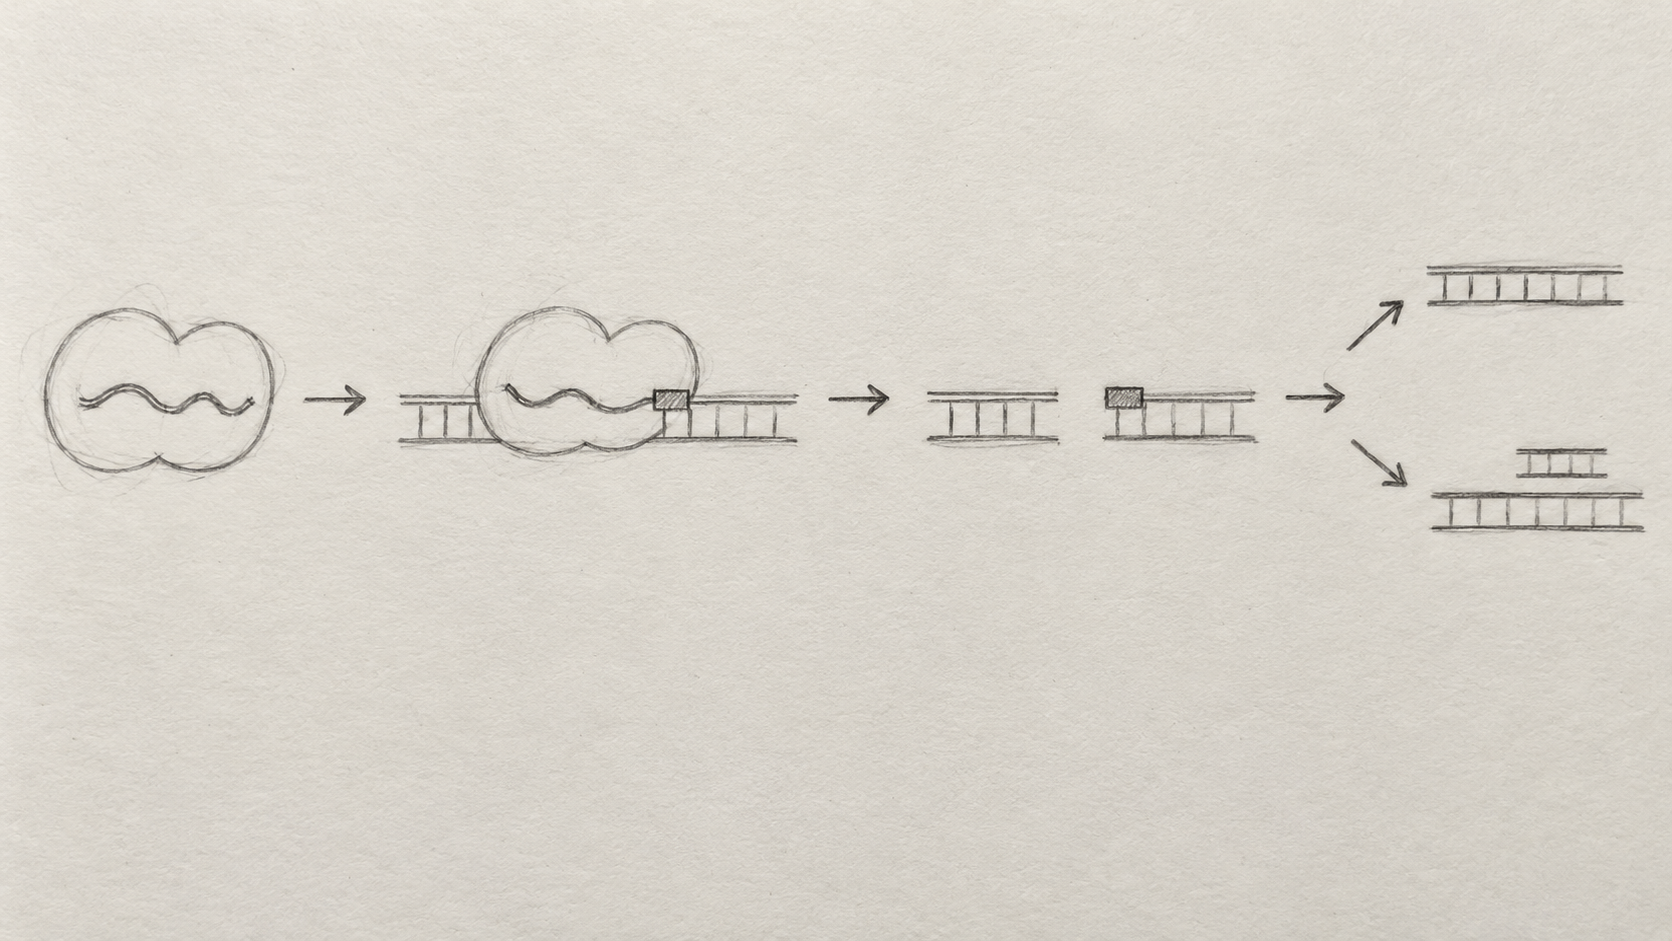
\includegraphics[width=\linewidth]{figures/ch03/ch03-02a-sketch-linear.png}};
\begin{scope}[x={(img.south east)},y={(img.north west)}]
  \node[font=\sffamily\bfseries\normalsize, anchor=north west, text=BookInk] at (0.04,0.94) {A};
\end{scope}
\end{tikzpicture}\\[1mm]
{\footnotesize A\quad 线性（左$\rightarrow$右）}
\end{minipage}\hfill
\begin{minipage}[t]{0.32\linewidth}\centering
\begin{tikzpicture}
\node[anchor=south west,inner sep=0] (img) at (0,0) {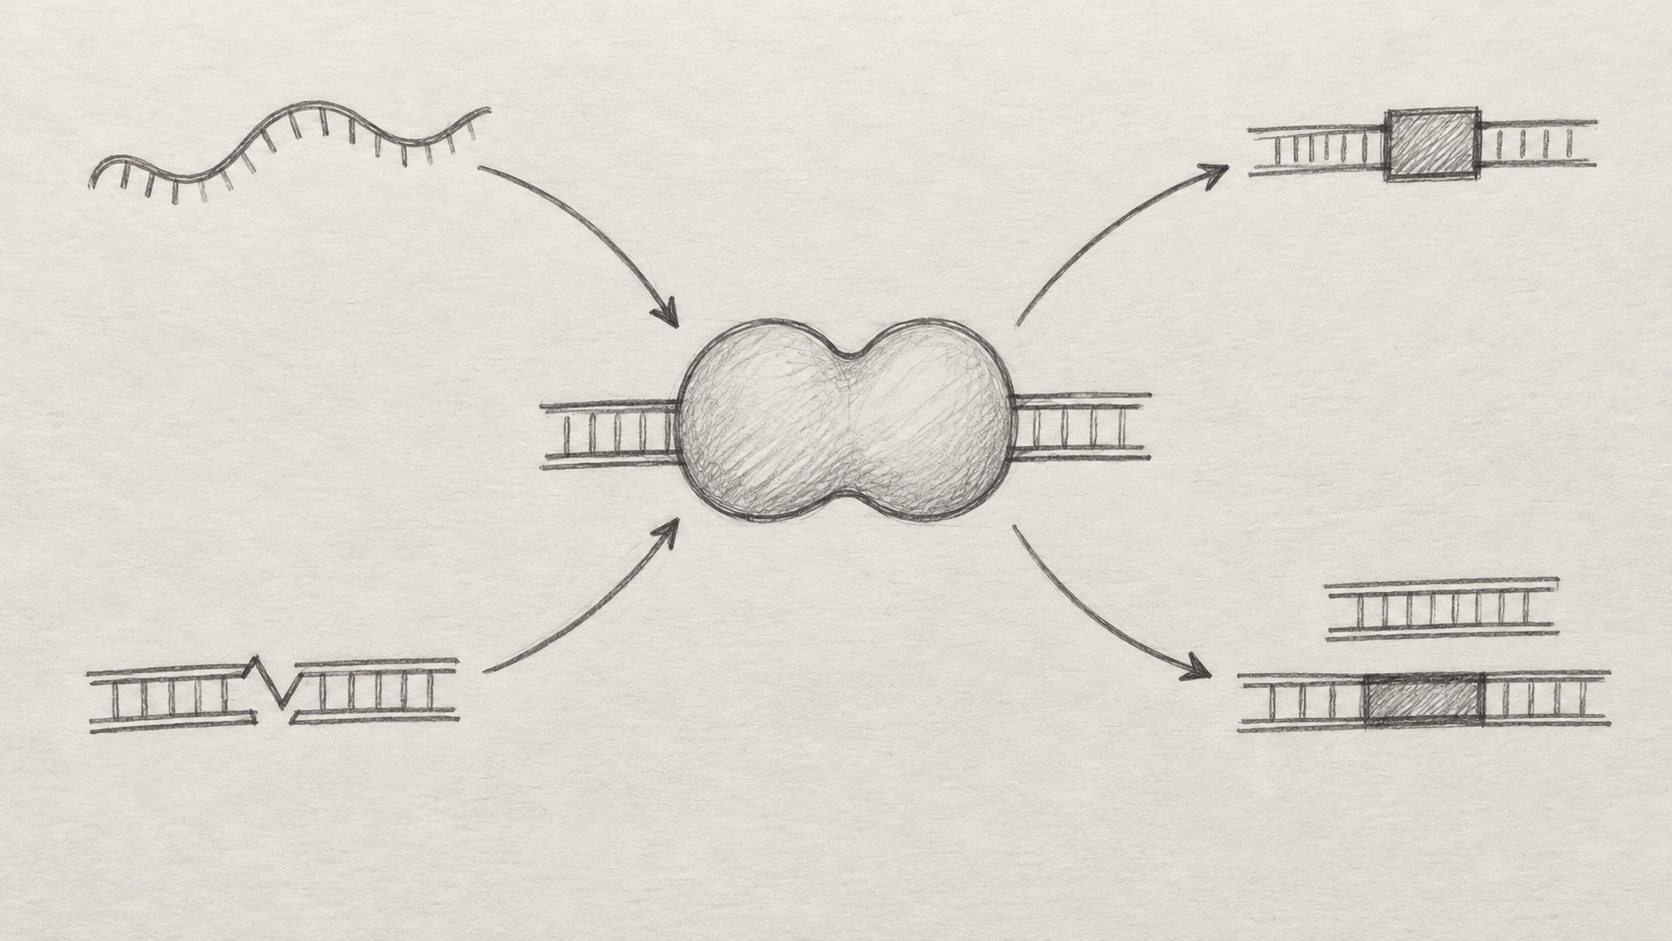
\includegraphics[width=\linewidth]{figures/ch03/ch03-02b-sketch-hub.png}};
\begin{scope}[x={(img.south east)},y={(img.north west)}]
  \node[font=\sffamily\bfseries\normalsize, anchor=north west, text=BookInk] at (0.04,0.94) {B};
\end{scope}
\end{tikzpicture}\\[1mm]
{\footnotesize B\quad 中心辐射}
\end{minipage}\hfill
\begin{minipage}[t]{0.32\linewidth}\centering
\begin{tikzpicture}
\node[anchor=south west,inner sep=0] (img) at (0,0) {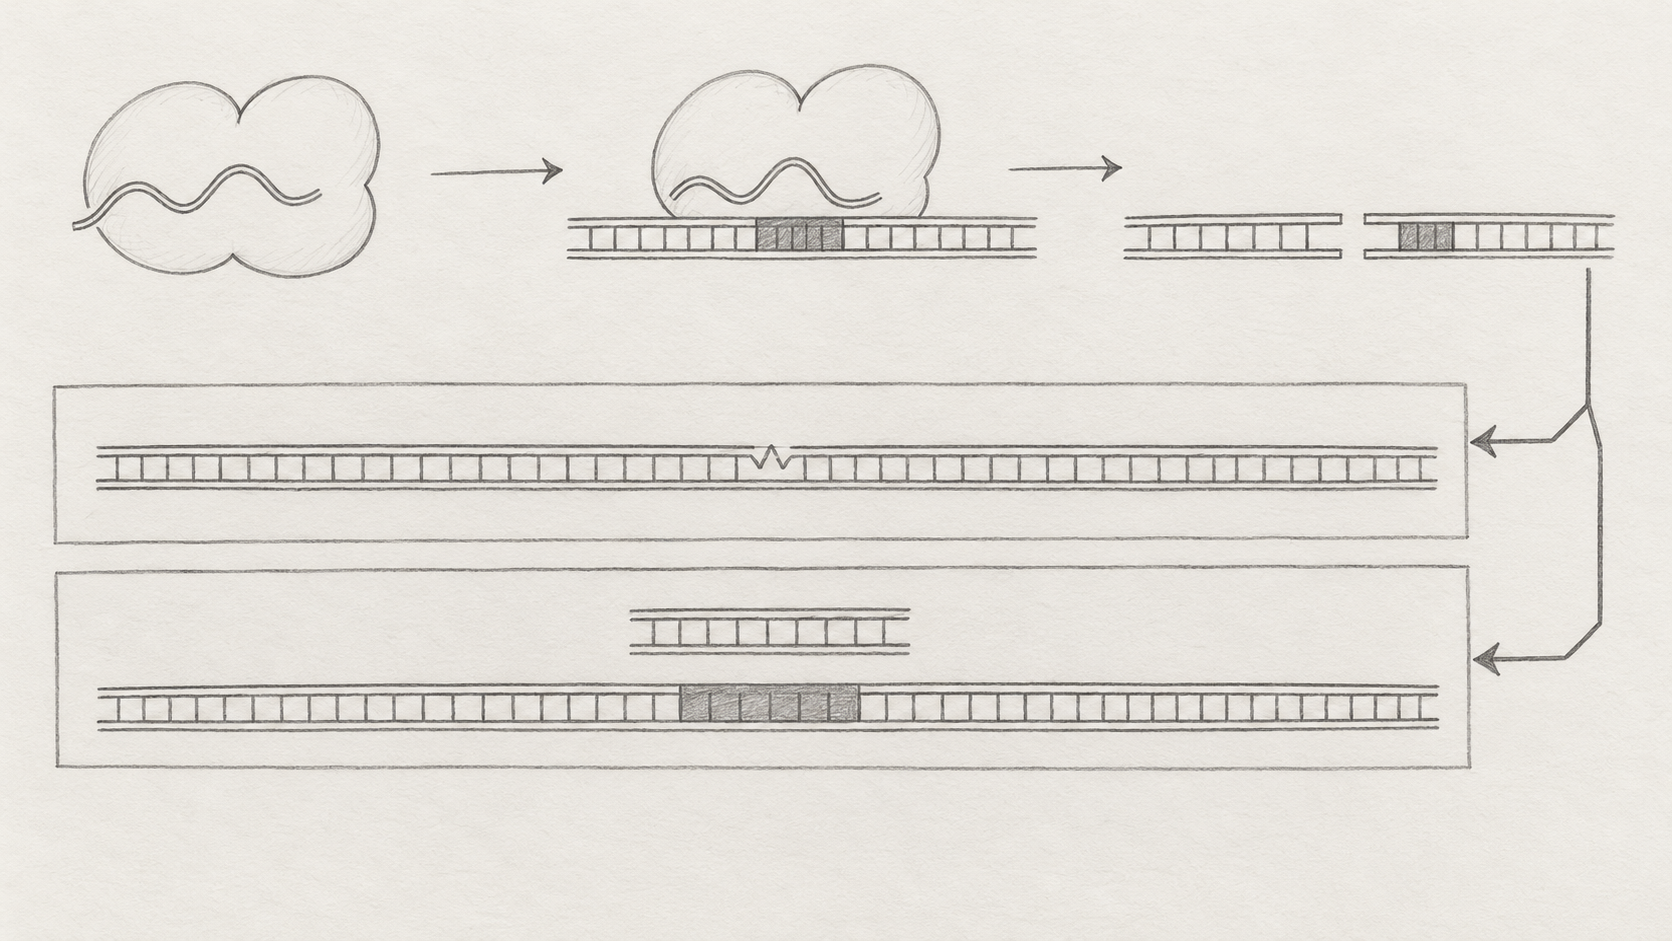
\includegraphics[width=\linewidth]{figures/ch03/ch03-02c-sketch-branch.png}};
\begin{scope}[x={(img.south east)},y={(img.north west)}]
  \node[font=\sffamily\bfseries\normalsize, anchor=north west, text=BookInk] at (0.04,0.94) {C};
\end{scope}
\end{tikzpicture}\\[1mm]
{\footnotesize C\quad 两分支结果}
\end{minipage}
\caption{同一内容的三种草图骨架（图像模型模拟的铅笔草图）。草图只确定分区、相对大小、箭头方向与留白，不写文字；对象的含义由任务书规定。A 把事件排成一行；B 以 Cas9–DNA 复合物为中心；C 把前三步压缩在上排，下方并列两条修复通道。本章示例图由图像模型生成，提示词与生成记录见本书仓库。}\label{fig:ch03-02}
\end{figure}

观察图~\ref{fig:ch03-02} 的生成过程与实际画面，可以总结出三点直接有用的经验：

第一，\textbf{线性单行最容易一次成形，但右端对比区天然局促。} 图~\ref{fig:ch03-02}A 第一次生成就排出了从左到右的四个阶段与右端分叉（阶段间以短箭头指示方向），但因前三步占去了左起大半宽度，右端上下叠放的两条结果双链被挤压得很短。

第二，\textbf{中心辐射结构天然抹平事件起点。} 生成图~\ref{fig:ch03-02}B 时，第一次抽样曾把左下角的 indel 折线画成了脱离 DNA 的大闪电，且箭头从右上、右下指向中心；第二次抽样恢复了贴附在双链上的小折线，四支单头箭头呈“左上与左下指向中心、中心指向右上与右下”的两进两出格局（中央蛋白铅笔排线较重），画面没有唯一入口。

第三，\textbf{模型对“分叉进入两个不同通道”的拓扑路由非常迟钝。} 生成图~\ref{fig:ch03-02}C 时，前两次抽样虽然画出了上排三步和下方两个铅笔矩形框，但模型连续两次把从第三步向下分叉出来的\textbf{两个箭头全部指在了上方通道框的上沿}，导致下方通道没有入口箭头，且上通道 DNA 中间裂成了大缺口。直到第三次抽样专门补充路由说明——要求分叉干线沿右侧框外下行，一支从右端进入上框，另一支继续向下从右端进入下框，且上框 DNA 保持连续只在中部画小折线——才得到图~\ref{fig:ch03-02}C 的正确连接。即便如此，仔细检查图~\ref{fig:ch03-02}C 仍可见上下两个铅笔框高度并不完全相等（下框略高），且左上蛋白内的 RNA 呈双描线。这说明作者自己拿铅笔在纸上花一分钟画出分叉箭头和等高通道，比纯靠文字让模型猜拓扑要高效得多。

送入下一步前，用四项标准自检每张草图：是否一眼能看出入口；分叉点是否清楚且两条结果画成并列；留白是否足够放标签；画面是否无文字。

\section{从草图到候选图，再到选择}

接着在 \scidraw{} 提示词绘图（\sdtool{ai-drawing}）中切换到\textbf{草图模式}，分别上传三张草图，粘贴同一份由任务书转化的英文提示词生成三张候选图。三次生成只替换上传的草图与末尾对应的布局句，而把视觉风格、对象颜色身份、步骤定义与禁止项保持一致，这样比较才公平。完整英文提示词分两段给出如下：

\begin{Prompt}
Flat 2D scientific overview schematic for a journal figure, landscape 16:9, pure white background. Clean vector illustration style: flat fills, thin dark gray outlines, no gradients, no shadows, no highlights, no 3D, no glow, no texture. ABSOLUTELY NO TEXT: no letters, no words, no numbers, no symbols, no labels, no legend, no title.
Follow the layout of the attached pencil sketch closely: same regions, same relative positions, same arrow directions.
OBJECTS (use these exact visual identities in every step where they appear):
- Cas9: a rounded two-lobed protein shape, muted blue-gray (#7C93A8).
- sgRNA: a single orange (#E69F00) strand with a short straight segment (the spacer) and a small hairpin loop scaffold, partly inside Cas9.
- Genomic DNA: two parallel dark gray (#4D4D4D) lines with short light gray rungs between them.
- PAM: a short bright yellow (#F0E442) segment on the upper DNA line.
- Double-strand break: a clean gap through both DNA lines, right next to the PAM.
- Donor template: a short separate double-stranded DNA; its two ends dark gray (homology arms), its middle segment teal (#009E73).
- NHEJ result: a continuous DNA with one small reddish-purple (#CC79A7) mark at the former break site.
- HDR result: a continuous DNA with a teal (#009E73) segment at the former break site, the same length as the donor's middle segment.
\end{Prompt}

\begin{Prompt}
STEPS: (1) Cas9 bound to sgRNA. (2) Cas9-sgRNA sitting on the DNA at the PAM, the orange spacer lying alongside the lower DNA line, the upper line slightly pushed away. (3) The DNA with the break next to the PAM, Cas9 lifted away. (4) Repair by end joining, giving the NHEJ result, with no donor. (5) Repair using the donor template, giving the HDR result; the donor appears only here. Steps are connected by solid dark gray arrows with filled heads; after step 3 the arrow splits into two equal arrows.
DO NOT DRAW: cells, nucleus, chromosomes, scissors, lightning, sparkles, double-helix twisting, realistic protein structure, any charts or data. Bottom 10% of the image empty.
LAYOUT [A]: one row of five steps left to right; steps 4 and 5 stacked at the right end.
LAYOUT [B]: radial; the DNA-bound Cas9 complex (step 2-3 merged) in the center, steps 1, 4, 5 and the PAM detail around it.
LAYOUT [C]: steps 1-3 as a compact row across the top third; below, two equal-height horizontal lanes stacked vertically, upper lane step 4, lower lane step 5, with the DNA in both lanes aligned at the same x positions and length.
\end{Prompt}

使用草图模式时必须明确一条边界：\textbf{草图是布局意图的强提示，而不是像素级布局锁定。} 模型在把铅笔草图渲染成彩色图形时，仍可能发生对象位置漂移、复制或身份互换。因此生成后必须先将候选图与原草图并排核对，再叠加阅读顺序编号（图~\ref{fig:ch03-03}）。

\begin{figure}[htbp]\centering
\begin{minipage}[t]{0.32\linewidth}\centering
\begin{tikzpicture}[ord/.style={circle, draw=orange!85!black, line width=0.6pt, fill=orange!15, inner sep=1pt, font=\sffamily\bfseries\scriptsize, text=BookInk}]
\node[anchor=south west,inner sep=0] (img) at (0,0) {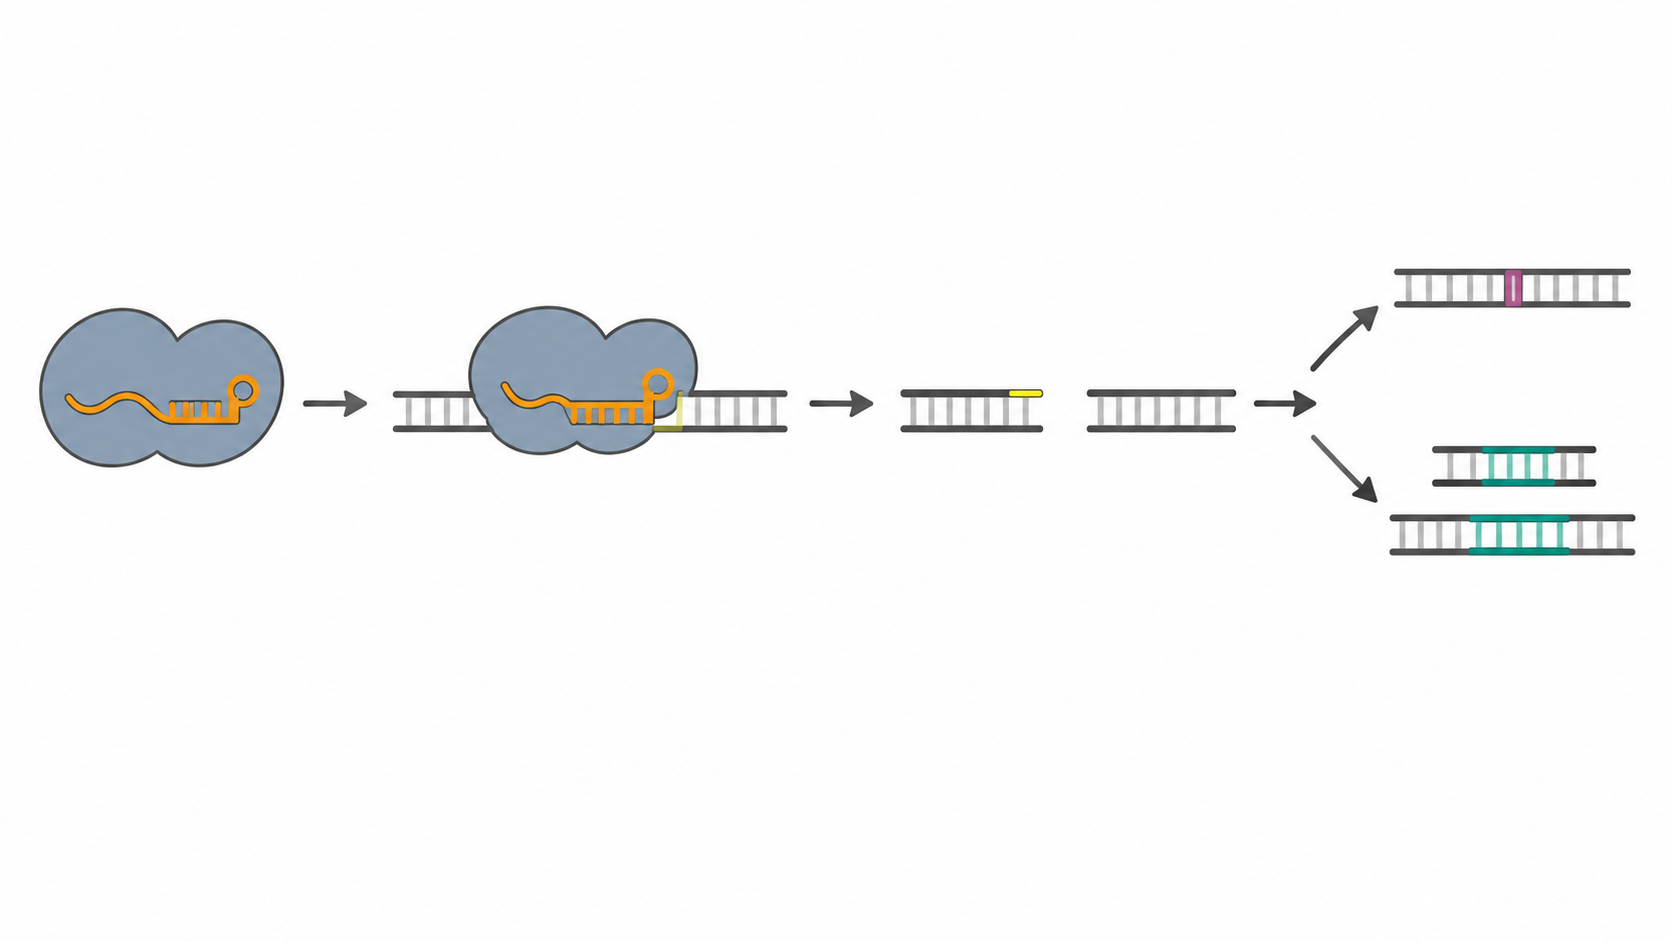
\includegraphics[width=\linewidth]{figures/ch03/ch03-03a-cand-linear.png}};
\begin{scope}[x={(img.south east)},y={(img.north west)}]
  \node[font=\sffamily\bfseries\normalsize, anchor=north west, text=BookInk] at (0.04,0.94) {A};
  \node[ord] at (0.08,0.55) {1};
  \node[ord] at (0.27,0.55) {2};
  \node[ord] at (0.46,0.55) {3};
  \node[ord] at (0.80,0.72) {4};
  \node[ord] at (0.80,0.35) {5};
\end{scope}
\end{tikzpicture}
\end{minipage}\hfill
\begin{minipage}[t]{0.32\linewidth}\centering
\begin{tikzpicture}[ord/.style={circle, draw=orange!85!black, line width=0.6pt, fill=orange!15, inner sep=1pt, font=\sffamily\bfseries\scriptsize, text=BookInk}]
\node[anchor=south west,inner sep=0] (img) at (0,0) {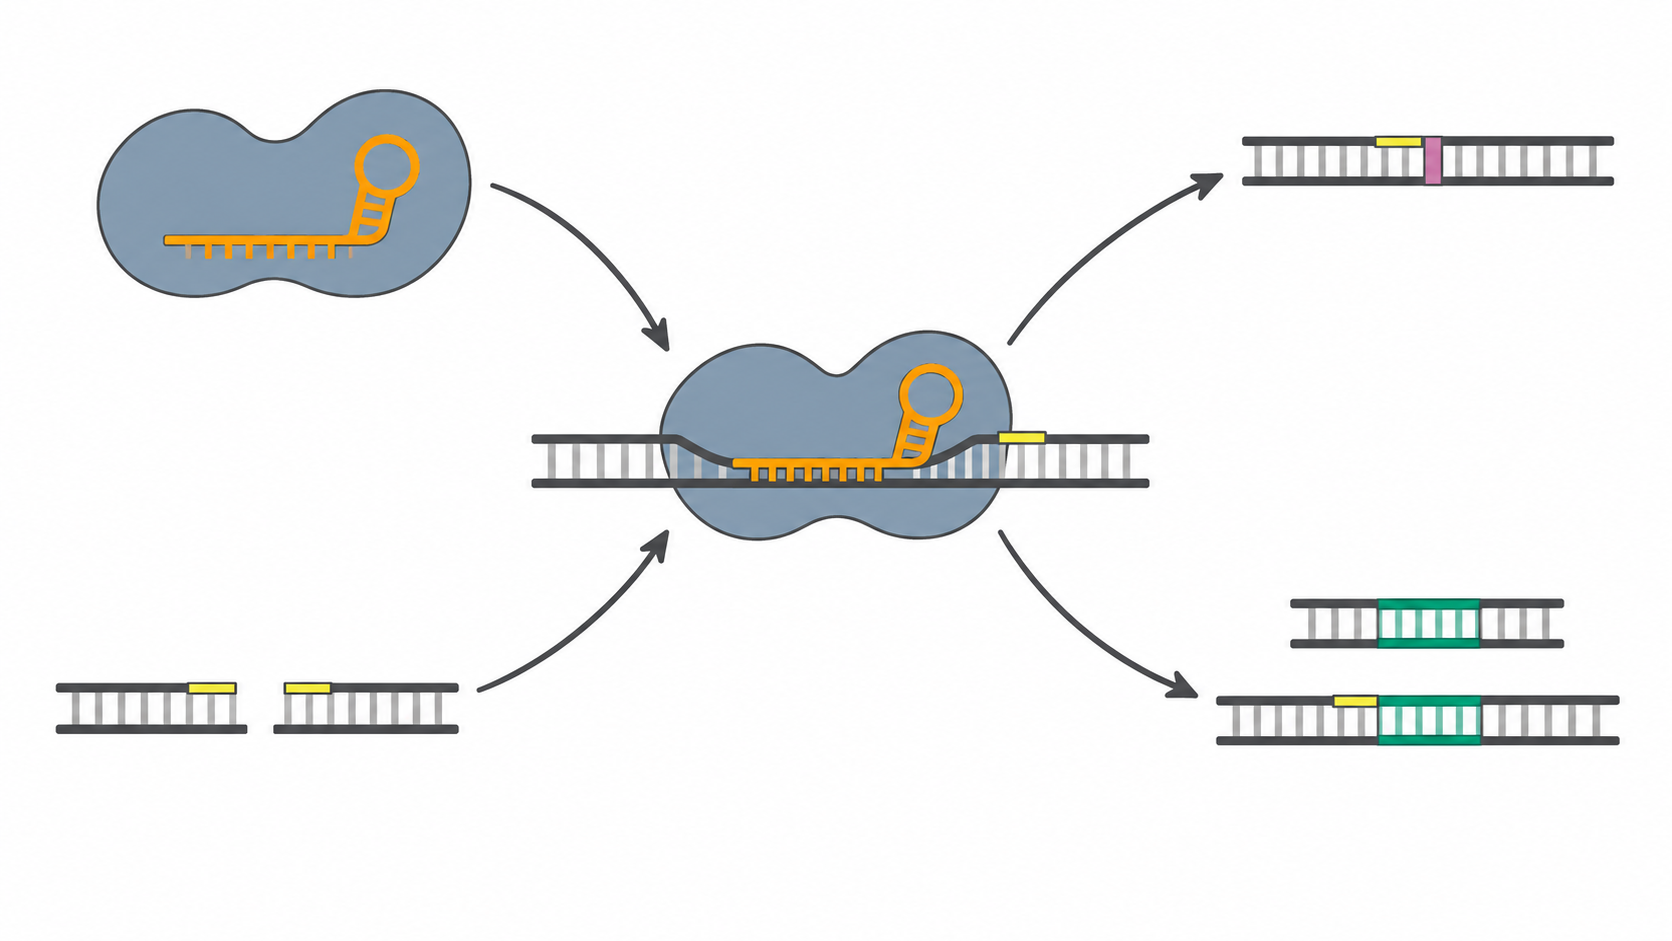
\includegraphics[width=\linewidth]{figures/ch03/ch03-03b-cand-hub.png}};
\begin{scope}[x={(img.south east)},y={(img.north west)}]
  \node[font=\sffamily\bfseries\normalsize, anchor=north west, text=BookInk] at (0.04,0.94) {B};
  \node[ord] at (0.50,0.52) {1?};
\end{scope}
\end{tikzpicture}
\end{minipage}\hfill
\begin{minipage}[t]{0.32\linewidth}\centering
\begin{tikzpicture}[ord/.style={circle, draw=orange!85!black, line width=0.6pt, fill=orange!15, inner sep=1pt, font=\sffamily\bfseries\scriptsize, text=BookInk}]
\node[anchor=south west,inner sep=0] (img) at (0,0) {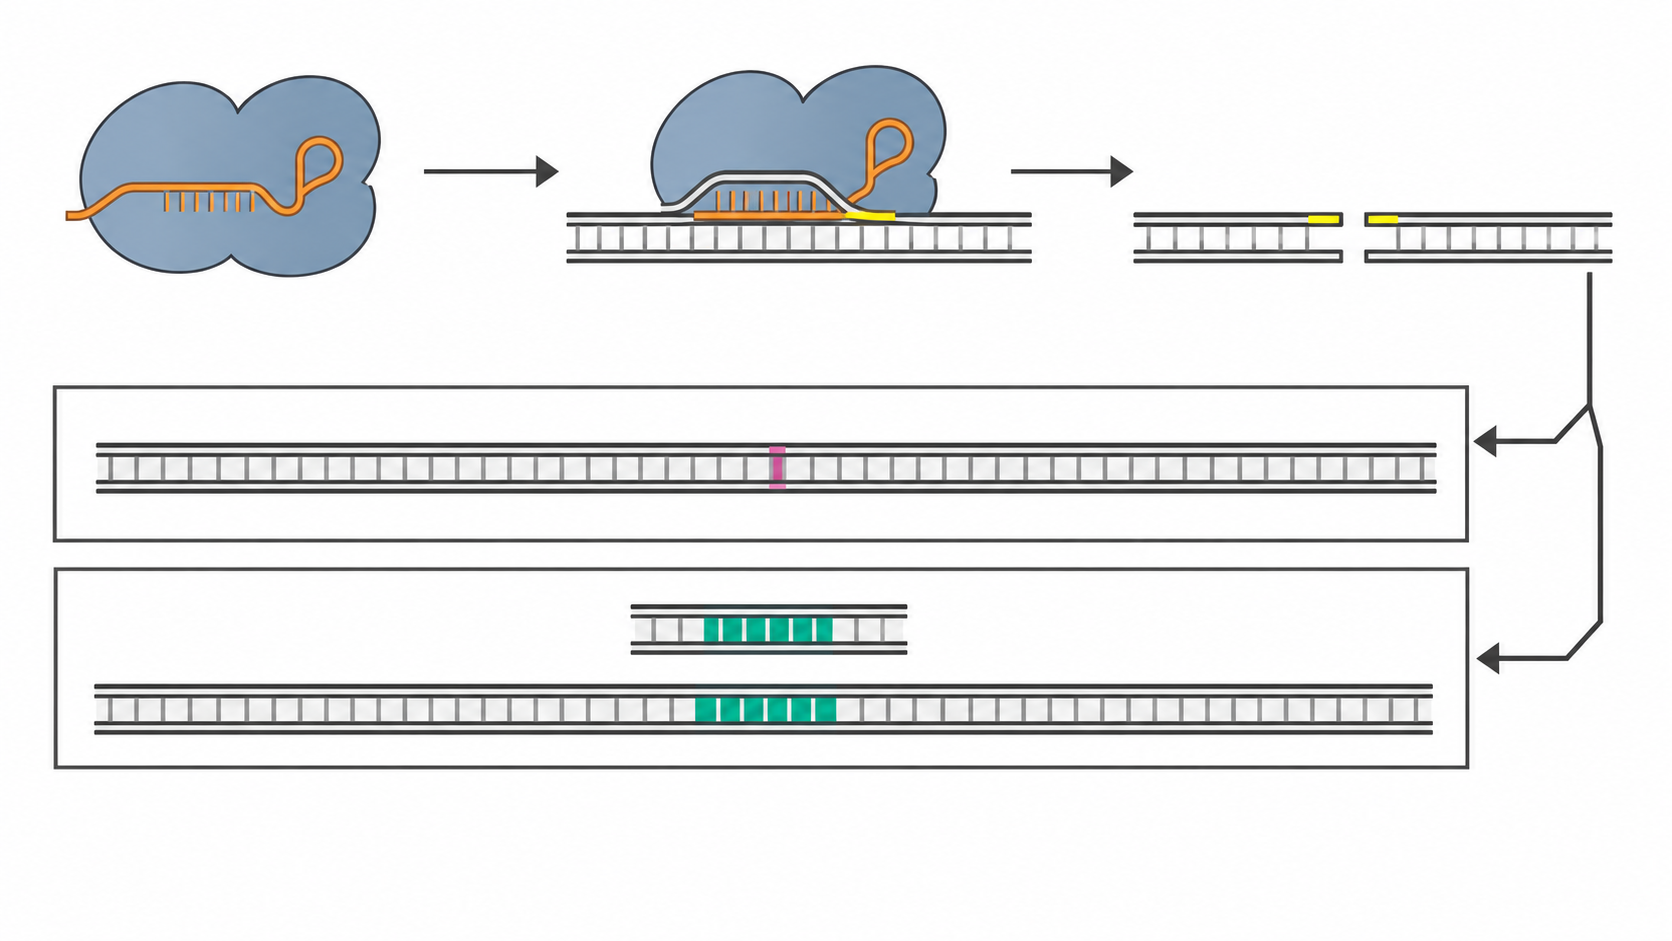
\includegraphics[width=\linewidth]{figures/ch03/ch03-03c-cand-branch.png}};
\begin{scope}[x={(img.south east)},y={(img.north west)}]
  \node[font=\sffamily\bfseries\normalsize, anchor=north west, text=BookInk] at (0.04,0.94) {C};
  \node[ord] at (0.15,0.85) {1};
  \node[ord] at (0.38,0.85) {2};
  \node[ord] at (0.62,0.85) {3};
  \node[ord] at (0.50,0.55) {4};
  \node[ord] at (0.50,0.22) {5};
\end{scope}
\end{tikzpicture}
\end{minipage}
\caption{同一份任务书、三张不同草图得到的候选图。橙色编号标出作者预期的阅读顺序（实际课题中应请未看过任务书的同事独立测试编号）：A 与 C 的顺序清晰且与事件先后一致；B 中左上与左下两支箭头同时指向中心，缺少唯一入口。生成后已对照草图核查位置偏离。}\label{fig:ch03-03}
\end{figure}

逐张对照图~\ref{fig:ch03-02} 与图~\ref{fig:ch03-03} 的实际画面，我们可以清楚看到三种骨架的表现及位置偏离：

\begin{itemize}
\item \textbf{候选 A（线性，图~\ref{fig:ch03-03}A）：} 一次生成即遵循了草图 A 从左到右的单行排布，Cas9（蓝灰）、sgRNA（橙）、DNA（深灰）、PAM（亮黄）、indel（红紫）及供体与写入段（青绿）的颜色角色全部准确，供体仅出现在右下角。但对照草图 A 检查第三步（切割步骤）时，发现了一处典型的**位置漂移**：草图 A 中位于缺口**右侧**的 PAM 阴影块，在候选 A 中被模型移到了缺口**左侧**；同时第二步 R 环配对关系不够清晰，最右端上下叠放的两个结果区域十分拥挤，供体中段与写入段的青绿长度也未严格相等。
\item \textbf{候选 B（中心辐射，图~\ref{fig:ch03-03}B）：} 这张图生动证明了“不良布局骨架会连带诱发科学内容错误”。前两次生成时，模型先后擅自把左下箭头反转为向外（把左上变成伪入口，并将单条 sgRNA 扩画成完整 Cas9–sgRNA 复合物）或画成双向箭头；第三次补充“严格保留左上、左下向内，右上、右下向外四支单头箭头”的说明后，虽然箭头方向对上了草图，画面却发生了严重的**对象身份交换与标记增殖**：原本在草图左下角的 NHEJ 结果（红紫标记）跑到右上角去了，左下角变成了断裂 DNA；而且左下缺口左右两侧、右上红紫标记左侧及右下青绿写入段左侧全都多出了一段黄色 PAM，正中央复合物处反而看不出双链断裂。同时，把“sgRNA”“断裂 DNA”与“修复结果”画成围绕中心的同级卫星节点，彻底拉平了事件层级。
\item \textbf{候选 C（两分支，图~\ref{fig:ch03-03}C）：} 一次生成即完整保留了“上排紧凑三步 + 右侧分叉 + 下方上下并列双通道”的骨架，短双链供体准确地只出现在下方 HDR 通道内且居中于青绿写入段上方，两条结果长 DNA 的左右端点也高度对齐（水平误差不到链长的 0.3\%），未出现细胞核等排除对象。但放大检查仍能定位两处待改问题：第一，上排第三步双链断裂的\textbf{缺口左右两侧各出现了一段黄色 PAM}（重复画了两个 PAM）；第二，下方两个矩形通道框高度明显不等，下框比上框高出约 29\%（此外三张候选图的蛋白与橙线均带轻微明暗高光，未做到绝对平涂）。
\end{itemize}

在实际课题中，此时应把三张无编号的候选图拿给一至两位没看过任务书的同事，请他们凭直觉标出阅读顺序 1–5（也可以请能看图的对话式 AI 描述它会先看哪里作为辅助参考，但不能替代真人测试）。接着，用一张写明客观标准的比较表（表~\ref{tab:ch03-02-cmp} 与图~\ref{fig:ch03-04}）作出选择，而不是凭“哪张更顺眼”。

\begin{table}[htbp]\centering\footnotesize
\setlength{\tabcolsep}{3pt}
\renewcommand{\arraystretch}{1.15}
\caption{三种布局候选方案的比较表。}\label{tab:ch03-02-cmp}
\begin{tabularx}{\linewidth}{@{}>{\raggedright\arraybackslash}p{36mm}YYY@{}}
\toprule
\textbf{标准} & \textbf{A 线性} & \textbf{B 中心辐射} & \textbf{C 两分支} \\
\midrule
入口是否唯一明确 & 是（左端步骤 1） & 否（左上与左下两进两出） & 是（左上角步骤 1） \\
阅读方向与事件先后一致 & 是 & 部分（需完全靠箭头，且对象错位） & 是 \\
两种结果能否在同一基线上直接对照 & 否（上下挤在右端） & 否（分散在右上与右下角） & 是（上下并列宽通道，端点对齐） \\
主要信息（同一断裂、两种结果）的视觉权重 & 低（占右端约 11\%--25\%） & 中（分散在角落，约 25\%） & 高（占下半幅约 50\%） \\
174 mm 宽下的标签空间 & 紧 & 中 & 足 \\
适合的用途 & 幻灯片逐步展示 & 概念关系图（非时序） & 论文总览图 \\
\bottomrule
\end{tabularx}
\end{table}

\begin{figure}[htbp]\centering
\resizebox{\linewidth}{!}{% FIG ch03-04 layout comparison (Chinese)
\begin{tikzpicture}[
  x=1mm, y=1mm,
  font=\sffamily\footnotesize,
  text=BookInk,
  wf/.style={draw=black!50, fill=black!4, line width=0.4pt},
  main/.style={fill=teal!25, draw=none},
]
  \def\fw{52}\def\fh{33}
  \begin{scope}[shift={(0,58)}]
    \draw[wf] (0,0) rectangle (\fw,\fh);
    \fill[main] (0.68*\fw,0.05*\fh) rectangle (0.96*\fw,0.43*\fh);
    \node[anchor=north, font=\bfseries] at (0.5*\fw,\fh+2) {A};
    \node[font=\scriptsize, anchor=south] at (0.5*\fw,-1.5) {约 11\%};
  \end{scope}
  \begin{scope}[shift={(56,58)}]
    \draw[wf] (0,0) rectangle (\fw,\fh);
    \fill[main] (0.15*\fw,0.12*\fh) rectangle (0.85*\fw,0.47*\fh);
    \node[anchor=north, font=\bfseries] at (0.5*\fw,\fh+2) {B};
    \node[font=\scriptsize, anchor=south] at (0.5*\fw,-1.5) {约 25\%};
  \end{scope}
  \begin{scope}[shift={(112,58)}]
    \draw[wf] (0,0) rectangle (\fw,\fh);
    \fill[main] (0,0) rectangle (\fw,0.50*\fh);
    \node[anchor=north, font=\bfseries] at (0.5*\fw,\fh+2) {C};
    \node[font=\scriptsize, anchor=south] at (0.5*\fw,-1.5) {约 50\%};
  \end{scope}
  \node[font=\scriptsize, text=BookInk!70, anchor=north west] at (0,54)
    {青绿区为两种修复结果所占面积（线框示意；候选 PNG 实测后更新）};

  \matrix (m) [
    matrix of nodes,
    anchor=north west,
    row sep=1.8mm,
    column sep=3mm,
    nodes={font=\scriptsize, inner sep=2pt},
    column 1/.style={nodes={anchor=west}, text width=38mm},
    column 2/.style={nodes={anchor=center}, text width=12mm},
    column 3/.style={nodes={anchor=center}, text width=12mm},
    column 4/.style={nodes={anchor=center}, text width=12mm},
  ] at (0,48) {
    & {A} & {B} & {C} \\
    入口唯一 & {$\bullet$} & {$\circ$} & {$\bullet$} \\
    顺序与事件一致 & {$\bullet$} & {\tikz[baseline=-0.6ex]{\fill[BookTeal] (0,0) arc (90:270:0.35); \draw[BookTeal] (0,0) circle (0.35);}} & {$\bullet$} \\
    两种结果可直接对照 & {$\circ$} & {$\circ$} & {$\bullet$} \\
    主要信息的面积 & {$\circ$} & {\tikz[baseline=-0.6ex]{\fill[BookTeal] (0,0) arc (90:270:0.35); \draw[BookTeal] (0,0) circle (0.35);}} & {$\bullet$} \\
    174\,mm 下标签空间 & {\tikz[baseline=-0.6ex]{\fill[BookTeal] (0,0) arc (90:270:0.35); \draw[BookTeal] (0,0) circle (0.35);}} & {\tikz[baseline=-0.6ex]{\fill[BookTeal] (0,0) arc (90:270:0.35); \draw[BookTeal] (0,0) circle (0.35);}} & {$\bullet$} \\
    适合的用途 & {幻灯片} & {概念图} & {论文总览} \\
  };
  \draw[BookTeal, line width=0.8pt, rounded corners=1pt]
    ([xshift=-2mm,yshift=2mm]m-1-4.north west) rectangle ([xshift=2mm,yshift=-2mm]m-7-4.south east);
\end{tikzpicture}
}
\caption{按写明的标准比较三种布局。上：线框中青绿区域为“两种修复结果”所占版面面积比例示意。下：逐项判定矩阵。选择 C 作为论文总览图；A 保留用于汇报幻灯片的逐步呈现。}\label{fig:ch03-04}
\end{figure}

如图~\ref{fig:ch03-04} 所示，本图的主要信息是“同一断裂、两种修复结果”，布局 C 将下半幅约 50\% 的版面完整分配给两条对齐的修复通道，读者能在同一水平位置直接比较 indel 与精确写入。因此我们在修改记录中写明选择理由：\textbf{选定 C 作为论文总览图；保留 A 用于汇报幻灯片的逐步动画版本；淘汰 B。}

\section{每次只改一个可核对的目标}

以候选 C 为起点进入修改阶段时，切忌下达“把细节改对、通道对齐、画面更简洁”的混合指令。参考图修改（在 \scidraw{} 中选中历史图并输入修改指令）本质上是条件重绘而非矢量软件的局部平移；如果一条指令里塞进三四个目标，不仅容易顾此失彼，而且一旦出现新错误，你根本无法判断是哪句话触发了模型的误操作。

正确的修订纪律是：\textbf{每次只提出一个可核对的目标，采用“具体改动目标 + 保持不变的内容 + 检查方法”的格式，并在每次修改后与上一版叠图对比，如实填写意外变化日志。}

我们先在候选 C（图~\ref{fig:ch03-05} 左）上对四个预设核查点（编号 1 至 4）做定点诊断，区分真问题与已达标项：

\begin{itemize}
\item \textbf{核查点 1（PAM 位置）：} 上排右侧切割步骤的缺口左右两侧各有一段黄色 PAM，左侧那段属于重复错误，\textbf{必须擦除左侧黄段、只保留右侧上链紧邻缺口的 PAM}。
\item \textbf{核查点 2（供体模板位置）：} 事先担心供体漂在通道之间或出现两次；实测候选 C 中短双链供体已经唯一地位于下方 HDR 通道内且大致居中。为检验单目标微调并使其青绿中段与写入段严格居中对齐，我们仍执行一次微调指令。
\item \textbf{核查点 3（两条通道对齐）：} 实测下方两条长 DNA 的左右端点水平误差已小于 0.3\%（满足 $<2\%$ 的要求），但\textbf{两个矩形通道外框的高度相差约 29\%}（下框明显高于上框），需要把两框高度调齐。
\item \textbf{核查点 4（多余背景对象）：} 事先准备了第 4 条指令用于删除可能出现的细胞核轮廓或装饰背景；实测候选 C 背景干净、无任何多余对象，因此\textbf{第 4 条修改指令直接跳过不执行}。
\end{itemize}

四条预设单目标修改指令的英文原文如下：

\begin{Prompt}
[Revision 1 - PAM position] Edit the selected image. Change only one thing: move the small yellow PAM segment so that it sits directly next to the right side of the DNA gap at the cleavage step, on the upper strand, touching the gap. Keep every other object, color, line weight and position unchanged. Do not add any text.
\end{Prompt}

\begin{Prompt}
[Revision 2 - Donor placement] Edit the selected image. Change only one thing: move the short teal donor DNA so that it lies inside the lower repair lane only, directly above the DNA gap in that lane, horizontally centered on the gap. Remove any copy of the donor outside the lower lane. Keep everything else unchanged. No text.
\end{Prompt}

\begin{Prompt}
[Revision 3 - Lane alignment] Edit the selected image. Change only one thing: make the two repair lanes the same height, and draw the DNA in both lanes at the same horizontal position and the same length, so the two results line up vertically for comparison. Keep colors, objects and the top row unchanged. No text.
\end{Prompt}

\begin{Prompt}
[Revision 4 - Remove extra objects, conditional] Edit the selected image. Remove the cell nucleus outline and any background shapes. Change nothing else. No text.
\end{Prompt}

\begin{figure}[htbp]\centering
\begin{minipage}[t]{0.49\linewidth}\centering
\begin{tikzpicture}[font=\sffamily\footnotesize, text=BookInk]
  \node[inner sep=0, anchor=south west] (imga) at (0,0) {%
    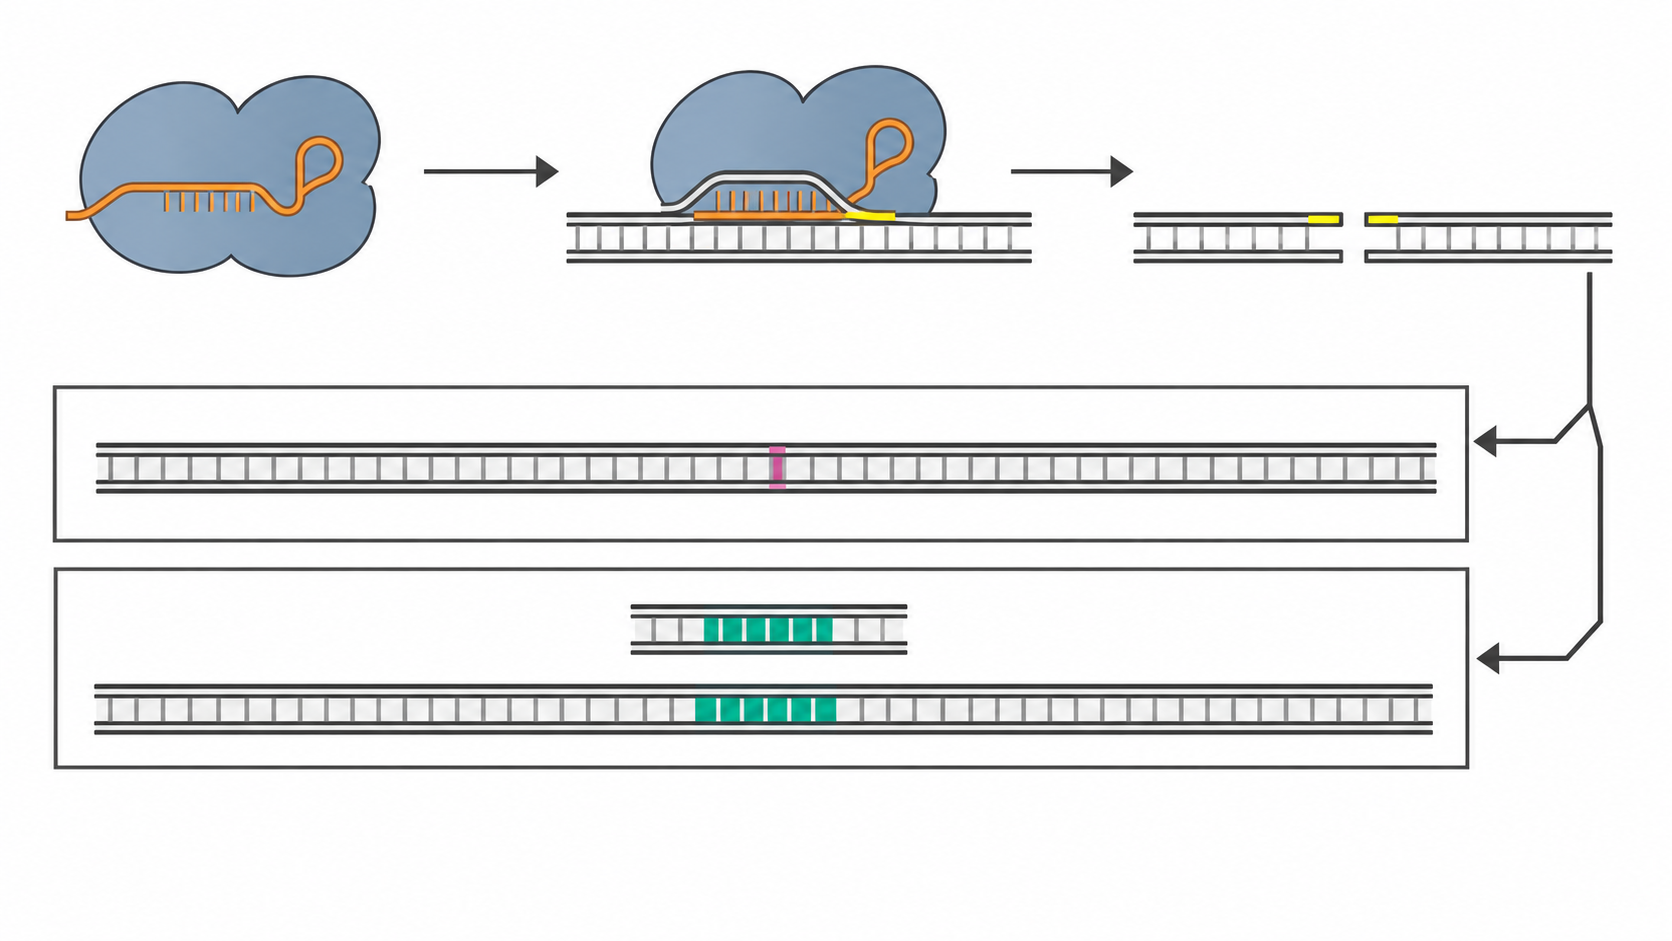
\includegraphics[width=\linewidth]{figures/ch03/ch03-03c-cand-branch.png}};
  \begin{scope}[x={(imga.south east)},y={(imga.north west)},
    issuemark/.style={circle, draw=red!75!black, line width=0.6pt, fill=white, fill opacity=0.88, text opacity=1, inner sep=0.8pt, font=\sffamily\bfseries\scriptsize, text=red!75!black}]
    \node[issuemark] at (0.62,0.78) {1};
    \node[issuemark] at (0.48,0.42) {2};
    \node[issuemark] at (0.72,0.28) {3};
    \node[issuemark] at (0.88,0.65) {4};
    \node[anchor=west, align=left, font=\sffamily\scriptsize] at (0.02,0.08) {%
      1 PAM 位置\quad 2 供体模板位置\\
      3 通道未对齐\quad 4 多余对象排查};
  \end{scope}
\end{tikzpicture}
\end{minipage}\hfill
\begin{minipage}[t]{0.49\linewidth}\centering
\begin{tikzpicture}[font=\sffamily\footnotesize, text=BookInk]
  \node[inner sep=0, anchor=south west] (imgb) at (0,0) {%
    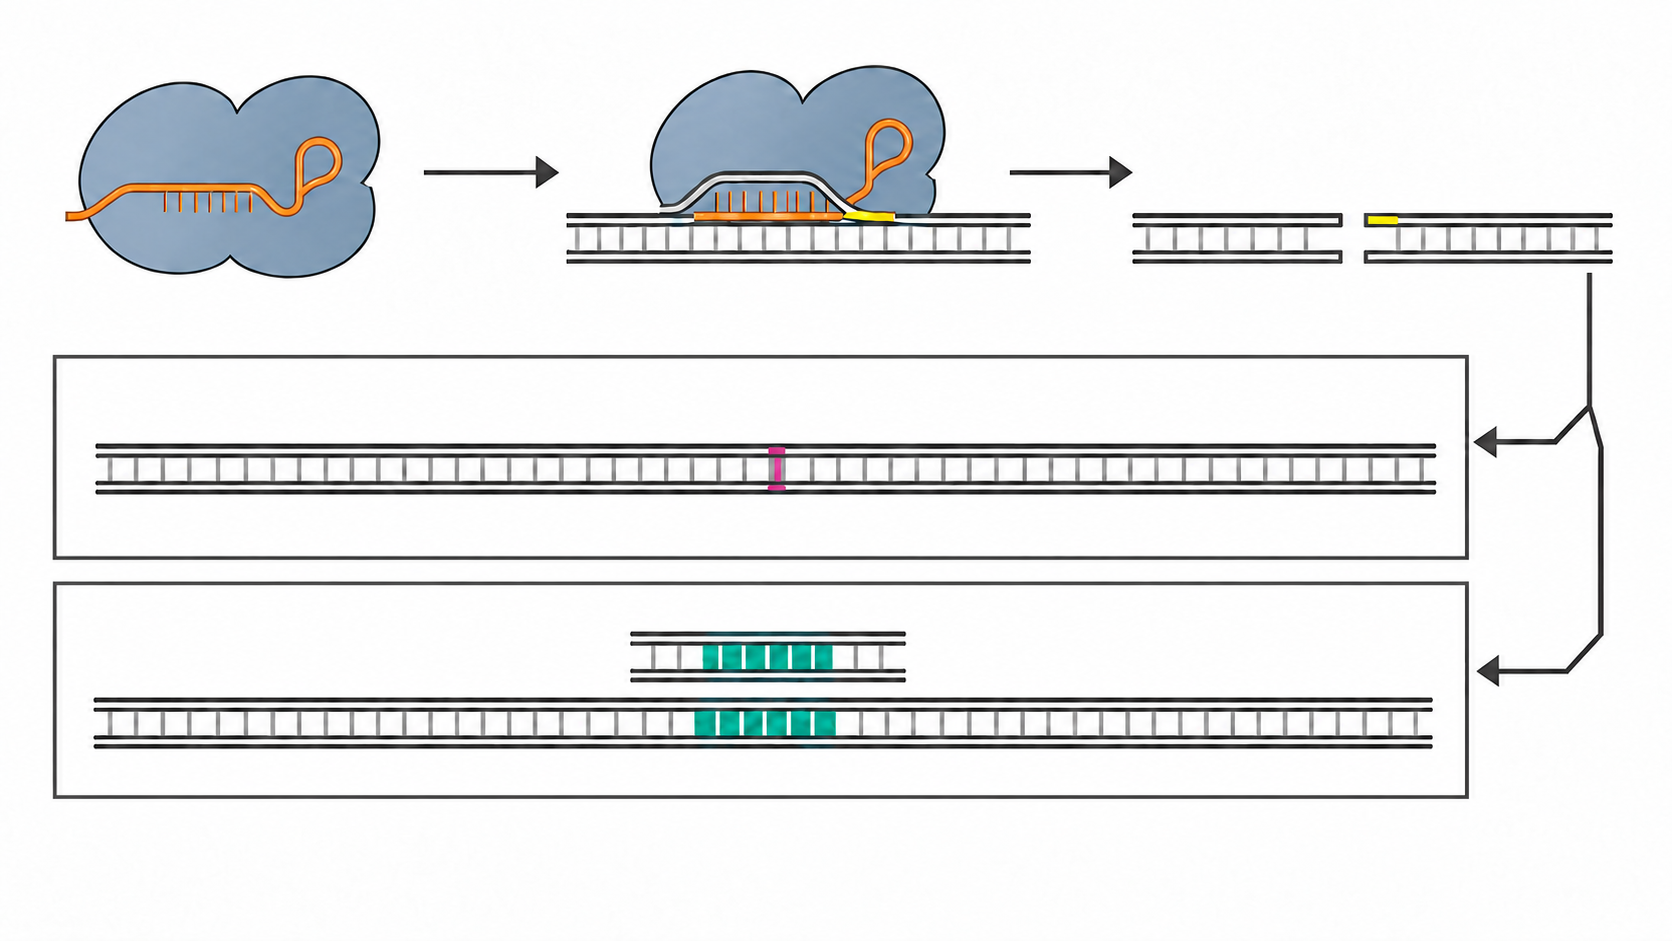
\includegraphics[width=\linewidth]{figures/ch03/ch03-05b-v3-revised.png}};
  \begin{scope}[x={(imgb.south east)},y={(imgb.north west)}]
    \draw[green!55!black, line width=0.8pt] (0.14,0.80) circle (0.07);
    \draw[green!55!black, line width=0.8pt] (0.48,0.29) circle (0.09);
    \node[anchor=west, align=left, font=\sffamily\scriptsize, text=green!45!black] at (0.02,0.08) {%
      意外变化：sgRNA 高光重绘、\\
      下通道微移及残留约 6\% 框高差};
  \end{scope}
\end{tikzpicture}
\end{minipage}
\caption{逐条修改。左：候选 C 的四个核查点，其中 1 处切口两侧重复画出黄色 PAM，3 处两通道外框高度明显不等（2 处供体已在下通道内，4 处实测无多余背景对象）。右：依次执行单目标修改后的版本；切口左侧重复 PAM 已消除，两框高度差大幅缩小；绿色圆圈标出未要求却发生的轻微重绘与位移，已记入修改记录。}\label{fig:ch03-05}
\end{figure}

表~\ref{tab:ch03-03-log} 完整记录了从候选 C 到图~\ref{fig:ch03-05} 右的七次真实调用与意外变化处理过程：

\begin{table}[htbp]\centering\footnotesize
\setlength{\tabcolsep}{3pt}
\renewcommand{\arraystretch}{1.15}
\caption{从候选 C 到修订稿的意外变化日志。}\label{tab:ch03-03-log}
\begin{tabularx}{\linewidth}{@{}>{\raggedright\arraybackslash}p{24mm}ccY>{\raggedright\arraybackslash}p{20mm}@{}}
\toprule
\textbf{修改阶段} & \textbf{尝试} & \textbf{达成} & \textbf{未要求却发生的变化（及是否影响科学）} & \textbf{处理决定} \\
\midrule
修改 1：PAM 位置 & 1 & 否 & 切口两侧仍有两个黄色 PAM；细线轻微再渲染（不影响科学） & 退回候选 C \\
修改 1：补充定位 & 2 & \textbf{是} & 左侧重复 PAM 消除；细描边与色彩纹理轻微再渲染（无影响） & \textbf{保留}为基准 1 \\
修改 2：供体居中 & 1 & 否 & \textbf{下通道内唯一的短双链供体被直接删掉（影响科学）} & \textbf{弃用}，退回基准 1 \\
修改 2：保护供体 & 2 & \textbf{是} & 供体保留并与青绿段对齐；供体整体下移约 15 像素（无影响） & \textbf{保留}为基准 2 \\
修改 3：通道等高 & 1 & 部分 & \textbf{供体消失；两条结果 DNA 均出现红紫和青绿（影响科学）} & \textbf{弃用}，退回基准 2 \\
修改 3：保护身份 & 2 & 否 & 科学身份恢复，但下框被进一步拉高、下通道下移（几何未达标） & 弃用，退回基准 2 \\
修改 3：抬高上框 & 3 & \textbf{是} & 框高差由 29.4\% 降至 6.0\%，端点误差 0.22\%；下通道微移、sgRNA 高光微变（无影响） & \textbf{保留}为修订稿 \\
修改 4：删背景 & 0 & — & 画面无细胞核或多余背景形状 & 条件跳过 \\
\bottomrule
\end{tabularx}
\end{table}

从表~\ref{tab:ch03-03-log} 的真实记录中，可以提炼出三条直接指导日常作图的修改准则：

\textbf{第一，当原指令首次调用无效时，补充“当前哪里错了、擦除什么、保留什么”的具体定位。} 修改 1 第 1 次调用之所以无效，是因为切口右侧本来就有一段黄色 PAM，模型认为要求已满足而保留了左侧多余黄段；第 2 次明确补充“擦除缺口左侧黄色高亮并恢复为深灰 DNA 线、仅保留右侧上链紧贴缺口的一段黄色高亮”，立即一次奏效。

\textbf{第二，警惕局部修改引发“误删唯一对象”或“抹平对照差异”的严重副作用，一旦发生立即回退上一版。} 修改 2 第 1 次调用时，模型过度响应“Remove any copy”，竟把下通道里唯一的短双链供体删光了；修改 3 第 1 次调用时，模型过度响应“same height and length”，不仅删掉供体，还把上下两条结果 DNA 都画成了同时带红紫和青绿的混合体，直接毁掉了 NHEJ 与 HDR 的科学对照！遇到这种破坏科学内容的意外变化，绝不能在坏图上继续发指令打补丁，而必须\textbf{立即退回上一轮验证通过的基准版}，在指令中补上保护性约束（如“上通道只保留红紫 indel、无青绿无供体；下通道保留青绿写入段及上方唯一短供体，仅抬高上框顶边”）重新生成。

\textbf{第三，区分“科学硬伤”与“无害的渲染波动”，适时停手或切换确定性工具。} 图~\ref{fig:ch03-05} 右侧绿色细圈标出了三轮修改积累的轻微连带变化：上排 sgRNA 橙色高光与轮廓粗细微变、下通道整体微幅下移，且两框仍留有约 6.0\% 的高度差（较最初的 29.4\% 已大幅改善，长 DNA 左右端点误差仅 0.22\%）。由于这些变化完全不影响 C1–C9 的科学含义与视觉比对，将其记入日志后即可接受定稿。反之，若同一局部指令重试 3 次仍不断破坏其他关键对象，则应停止生成式修改，把精确几何交给 TikZ 绘制。

\section{案例收束：终稿、图注与核验}

为了在总览图右上角嵌入图~\ref{fig:ch03-07} 的确定性 PAM 细节插图，我们以图~\ref{fig:ch03-05} 右为参考图，执行最后一次版面留白调整，将上排三步向左紧凑移动，腾出右上角约 30\% 宽度的空白：

\begin{Prompt}
Edit the selected image. Change only one thing: shift the three steps of the top row to the left so that the right 30% of the top row is empty white space. Keep sizes, colors and the two lower lanes unchanged. No text.
\end{Prompt}

这一步同样经过三次抽样筛选：第 1 次右上仅腾出约 23\% 宽度且第三步与右侧分叉干线脱节；第 3 次虽留白充足，但模型把第三步连接线改为只指向 NHEJ 上框，与右侧双分支干线断开，破坏了“同一断裂分出两条途径”的路径拓扑；因此最终选定\textbf{第 2 次抽样}作为终稿无字底图——上排三步紧凑左移（伴随未要求的轻微缩小），折线从第三步顺畅接入右侧共同分叉干线，右上角腾出约 30\% 宽、约 32\% 高的无遮挡区域（仅底缘有一段水平连接线经过）。灰度检查表明，亮黄色 PAM（带深色描边）与青绿色供体存在显著明度对比，黑白打印下仍可清晰区分。

随后在 LaTeX/TikZ 中采用 book-spec 规范的相对坐标叠加写法，将图~\ref{fig:ch03-07} 缩放嵌入右上角空白区，并叠加全部中文矢量标签、步骤编号 1–5 与底部图例，合成终稿（图~\ref{fig:ch03-06}）。

\begin{figure}[htbp]\centering
\begin{tikzpicture}[font=\sffamily\scriptsize, text=BookInk]
  \node[anchor=south west, inner sep=0] (img) at (0,0) {%
    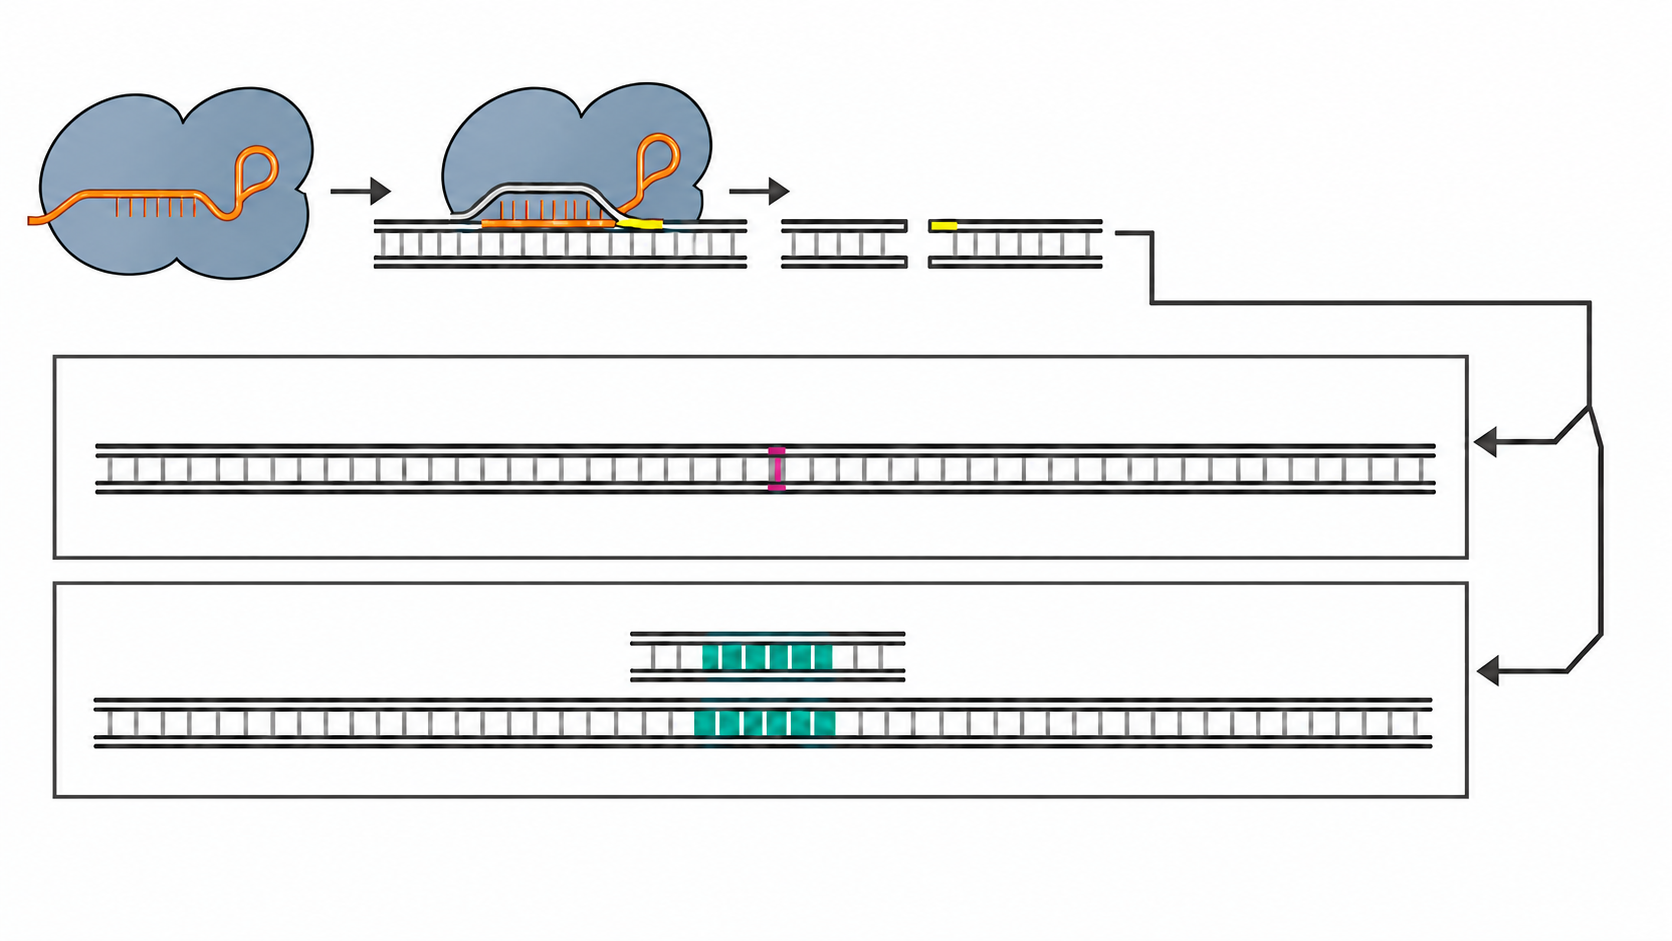
\includegraphics[width=\linewidth]{figures/ch03/ch03-06-final-base.png}};
  \begin{scope}[x={(img.south east)}, y={(img.north west)},
    lbl/.style={font=\sffamily\scriptsize, fill=white, fill opacity=0.88, text opacity=1, inner sep=1pt},
    ord/.style={circle, draw=orange!85!black, line width=0.5pt, fill=orange!15, inner sep=0.8pt, font=\sffamily\bfseries\tiny, text=BookInk}]
    \node[anchor=south west, inner sep=0, fill=white, fill opacity=0.92, text opacity=1] at (0.64,0.60) {%
      \resizebox{0.35\linewidth}{!}{% FIG ch03-07 PAM inset (Chinese)
\begin{tikzpicture}[
  x=1mm, y=1mm,
  font=\sffamily\scriptsize,
  text=BookInk,
]
  \node[anchor=east] at (-2, 21.2) {非靶链};
  \node[anchor=east] at (-2, 7.2) {靶链};
  \node at (6, 23.6) {5$'$};
  \node at (54.5, 23.6) {3$'$};
  \node at (55.5, 4.4) {5$'$};
  \node at (6, 4.4) {3$'$};

  \foreach \i in {0,...,19} {
    \pgfmathsetmacro{\x}{6+\i*2.4}
    \draw[draw=BookInk!50, fill=white] (\x,20) rectangle (\x+2.4,22.4);
  }
  \foreach \i in {0,1,2} {
    \pgfmathsetmacro{\x}{6+(17+\i)*2.4}
    \draw[draw=BookInk!50, fill=yellow!70] (\x,20) rectangle (\x+2.4,22.4);
  }
  \node[anchor=west, text=BookInk!80] at (6+17*2.4, 28.2) {PAM（NGG）};

  \foreach \i in {0,...,19} {
    \pgfmathsetmacro{\x}{6+\i*2.4}
    \draw[draw=BookInk!50, fill=white] (\x,6) rectangle (\x+2.4,8.4);
  }
  \foreach \i in {0,...,19} {
    \pgfmathsetmacro{\x}{6+\i*2.4}
    \draw[BookInk!35, thin] (\x+1.2,8.4) -- (\x+1.2,11.6);
    \draw[draw=orange!80!black, fill=orange!25, line width=1pt]
      (\x,4) rectangle (\x+2.4,6.4);
  }
  \draw[orange!80!black, line width=0.8pt]
    (6+19*2.4+2.4, 5) .. controls (6+21*2.4, 8) .. (6+21*2.4, 12)
    .. controls (6+21*2.4, 14) .. (6+19*2.4, 14);

  \node[anchor=west] at (6, 0.5) {sgRNA 间隔序列};
  \pgfmathsetmacro{\cx}{6+16.5*2.4+1.2}
  \fill[black] (\cx,20) -- (\cx-0.8,21.2) -- (\cx+0.8,21.2) -- cycle;
  \fill[black] (\cx,6) -- (\cx-0.8,4.8) -- (\cx+0.8,4.8) -- cycle;
  \node[anchor=west] at (6+17.5*2.4, 13) {切点};
  \node[anchor=west, font=\scriptsize] at (6+16*2.4, 17) {RuvC};
  \node[anchor=west, font=\scriptsize] at (6+16*2.4, 3) {HNH};

  \draw[decorate, decoration={brace, amplitude=3pt}] (6, 15.5) -- (6+20*2.4, 15.5)
    node[midway, above=4pt] {约 20 nt};
  \draw[decorate, decoration={brace, amplitude=2pt, mirror}] (6+16*2.4, 22.5) -- (6+17*2.4, 22.5)
    node[midway, below=2pt] {3 bp};
\end{tikzpicture}
}};
    \node[ord] at (0.04,0.92) {1};
    \node[ord] at (0.24,0.92) {2};
    \node[ord] at (0.46,0.82) {3};
    \node[ord] at (0.03,0.52) {4};
    \node[ord] at (0.03,0.22) {5};
    \node[lbl, font=\sffamily\bfseries\scriptsize] at (0.10,0.92) {Cas9};
    \node[lbl, font=\sffamily\bfseries\scriptsize] at (0.06,0.72) {sgRNA};
    \node[lbl] at (0.38,0.70) {PAM};
    \node[lbl] at (0.30,0.62) {靶 DNA};
    \node[lbl] at (0.52,0.62) {双链断裂};
    \node[lbl, anchor=west] at (0.06,0.48) {NHEJ（无模板）};
    \node[lbl, anchor=west] at (0.06,0.22) {HDR（供体模板）};
    \node[lbl] at (0.55,0.40) {小片段插入/缺失};
    \node[lbl] at (0.50,0.34) {供体模板};
    \node[lbl] at (0.55,0.12) {精确编辑};
    \node[font=\sffamily\scriptsize, align=left, anchor=north west] at (0.02,0.05) {%
      图例：实线箭头 = 步骤；分叉箭头 = 两种可选修复途径；黄色 = PAM；红紫 = indel；青绿 = 供体来源序列};
  \end{scope}
\end{tikzpicture}
\caption{CRISPR–Cas9 基因组编辑总览图终稿。无字底图叠加矢量标签、底部图例与右上角确定性 PAM 细节插图（图~\ref{fig:ch03-07}）。完整中英文图注见正文。}\label{fig:ch03-06}
\end{figure}

编写图注时，若使用 \scidraw{} 的图注辅助工具（\sdtool{figure-legend}）起草初稿，作者必须逐句核实简化声明与文献依据，严禁编造任何效率数值、样本量（\texttt{n=}）或统计显著性结论。完整的中英文图注如下：

\begin{BookNote}
\textbf{图 1　CRISPR–Cas9 基因组编辑及两种主要修复结果示意。} 单链引导 RNA（sgRNA）与 Cas9 结合；复合物识别基因组 DNA 上的 PAM（SpCas9 为 $5'$-NGG-$3'$），sgRNA 的约 20 nt 间隔序列与靶链配对，Cas9 在 PAM 上游约 3 bp 处切开两条链，形成双链断裂。断裂可经非同源末端连接（NHEJ）修复，该途径不需要模板，可能在断裂处留下小片段插入或缺失（indel），位于编码区时可能破坏基因功能；在提供带同源臂的供体模板时，也可经同源定向修复（HDR）按模板写入精确改变，HDR 在多数细胞中频率低于 NHEJ。插图示意 PAM、靶链、非靶链与切点的相对位置。为便于阅读，图中省略了 Cas9 的三维结构与 HNH/RuvC 结构域的分工（插图除外）、修复途径的分子因子、替代末端连接途径、脱靶切割及递送方式。依据 Jinek 等（2012）、Doudna 与 Charpentier（2014）、Hsu 等（2014）整理。

\medskip
\textbf{Figure 1 | Overview of CRISPR–Cas9 genome editing and its two main repair outcomes.} A single guide RNA (sgRNA) binds Cas9. The complex recognizes a protospacer-adjacent motif (PAM; $5'$-NGG-$3'$ for SpCas9) in genomic DNA, the $\sim$20-nt spacer of the sgRNA base-pairs with the target strand, and Cas9 cleaves both strands about 3 bp upstream of the PAM, creating a double-strand break. The break can be repaired by non-homologous end joining (NHEJ), which needs no template and may leave small insertions or deletions (indels) that can disrupt a coding sequence; when a donor template with homology arms is supplied, homology-directed repair (HDR) can instead copy a precise change from the template. In most cell types HDR is less frequent than NHEJ. The inset shows the positions of the PAM, the target and non-target strands and the cleavage site. For clarity, the three-dimensional structure of Cas9, the division of labour between the HNH and RuvC domains (except in the inset), repair factors, alternative end-joining pathways, off-target cleavage and delivery methods are omitted. Based on Jinek et al.\ (2012), Doudna and Charpentier (2014) and Hsu et al.\ (2014).
\end{BookNote}

最后，对照关系表 C1–C9 对终稿图~\ref{fig:ch03-06} 做逐条核验（表~\ref{tab:ch03-04-verify}）。

\begin{table}[htbp]\centering\footnotesize
\setlength{\tabcolsep}{3pt}
\renewcommand{\arraystretch}{1.15}
\caption{CRISPR–Cas9 总览图终稿核验记录表。}\label{tab:ch03-04-verify}
\begin{tabularx}{\linewidth}{@{}l>{\raggedright\arraybackslash}p{22mm}>{\raggedright\arraybackslash}p{34mm}cY@{}}
\toprule
\textbf{\#} & \textbf{关系} & \textbf{图中应见} & \textbf{结论} & \textbf{备注} \\
\midrule
C1 & sgRNA–Cas9 结合 & 步骤 1 两者接触成复合物 & $\checkmark$ & 橙色 sgRNA 与蓝灰 Cas9 接触，发夹可辨 \\
C2 & 识别 PAM & 步骤 2 复合物停在黄色 PAM 处 & $\checkmark$ & 复合物邻近亮黄色 PAM 段 \\
C3 & 间隔序列与靶链配对 & RNA 与一条 DNA 链平行贴合，另一条被推开 & 部分 & 底图有置换拱起但横档使配对链身份略含混；由右上角确定性插图精确阐明 \\
C4 & PAM 位置 & 黄色段在非靶链、紧邻配对区一端（插图精确） & $\checkmark$ & 底图切口右侧上链保留单一黄段；右上插图精确锁定非靶链 $3'$ 侧 $5'$-NGG-$3'$ \\
C5 & 双链断裂 & 两条链在同一处断开，紧邻 PAM & $\checkmark$ & 底图双链同处断开；上游约 3 bp 距离及 HNH/RuvC 分工由右上插图表达 \\
C6/C7 & NHEJ 结果 & 无模板；断裂处有红紫 indel 标记 & $\checkmark$ & 上通道 4 无模板，中部带单一红紫标记；图注写明“可能” \\
C8/C9 & HDR 结果 & 供体只在此通道；结果 DNA 含青绿写入段 & 部分 & 下通道 5 含唯一短供体及正下方青绿写入段（两段青绿长度接近，属示意表达） \\
— & 阅读顺序 & 1–5 编号路径与预期一致 & $\checkmark$ & 上排 1–3 接右侧分叉入 4–5；长 DNA 端点误差 0.22\%（正式提交前补同事盲测） \\
— & 禁止项 & 无细胞核、剪刀、发光、底图文字 & $\checkmark$ & 200\% 放大检查底图无文字及违禁对象 \\
— & 复核 & 由做基因编辑的同行签名复核 & 待完成 & 投稿前请基因编辑方向同行复核插图链方向、HNH/RuvC 标注与图注措辞 \\
\bottomrule
\end{tabularx}
\end{table}

回顾全过程，本案例归档的交付物涵盖：三张草图、三张候选图及偏离记录、比较表与选择理由、单目标修改指令与意外变化日志、确定性插图、无字底图与合成终稿、中英文图注及核验记录表。

\section{AI 在这一步能做什么与不能做什么}

构图推演与草图迭代环节中 AI 与作者的职责边界汇总于表~\ref{tab:ch03-01}。

\begin{table}[htbp]\centering\footnotesize
\setlength{\tabcolsep}{3pt}
\renewcommand{\arraystretch}{1.15}
\caption{AI 在构图与草图环节能做什么、不能做什么及作者要核对的内容。}\label{tab:ch03-01}
\begin{tabularx}{\linewidth}{@{}>{\raggedright\arraybackslash}p{20mm}YYY@{}}
\toprule
\textbf{环节} & \textbf{AI 能做} & \textbf{AI 不能做 / 不可靠} & \textbf{作者要核对} \\
\midrule
提出布局骨架 & 对话式 AI 可按任务书用文字列出几种布局思路及其阅读顺序 & 不会自动根据论文判断哪种布局最好；\scidraw{} 的批量候选共享同一提示词，结构差异有限，不会独立规划不同方案并解释理由 & 至少有一个骨架是自己画的；三种骨架在结构上真的不同 \\
草图 $\rightarrow$ 候选图 & \scidraw{} 草图模式可把草图与提示词一起作为输入，较快得到遵循大致布局的候选图 & 草图不等于布局锁定：对象可能漂移、合并、缺失、新增或互换身份 & 对照草图逐项检查位置、方向、数量；记录偏离 \\
阅读顺序评估 & 可请能看图的对话式 AI 描述“它会先看哪里”，作为一个额外视角 & 模型的描述不等于真实读者的视线；不能代替同行测试 & 至少请一位没看过任务书的人编号；以人的结果为准 \\
选择布局 & 可帮助把比较标准整理成表格 & 不能替作者决定什么是主要信息 & 主要信息写在任务书里；选择理由写进修改记录 \\
修改 & 参考图修改可按指令调整位置、删除对象、改外框或颜色 & 局部指令可能引起连带变化；同一指令结果不稳定；无法精确控制几何关系（链方向、碱基距离） & 每次一个目标；与上一版叠图比较；填写意外变化日志；精确几何改用 TikZ \\
科学正确性 & 能按给定关系画出示意 & 不会自己发现 PAM 画错链、切点离 PAM 太远、供体或颜色标记混淆 & 按关系表 C1–C9 逐条核验；领域同行复核 \\
文字与标签 & —（底图要求无文字） & 生成图中的文字常拼错、错位 & 标签在 LaTeX/TikZ 中叠加，作者校对拼写与位置 \\
\bottomrule
\end{tabularx}
\end{table}

\section{本章检查清单}

\begin{itemize}
\item 我能用一句话说出这张图的入口、路径和终点。
\item 图中只有一个视觉最重的元素，而且它承载主要信息。
\item 放在同一组（接近、对齐、围合）的对象确实相关；无关对象没有被意外分到一组。
\item 分叉处两条路径画成并列选项，读者不会误以为是先后步骤。
\item 需要精确几何关系的细节（链方向、位置、距离）用确定性工具绘制，或单独成插图。
\item 我画了至少三种结构不同的草图，并保存了它们。
\item 生成候选图时，每次只换草图、不换任务书核心文字。
\item 我对照草图记录了每张候选图的位置偏离。
\item 阅读顺序由至少一位没看过任务书的人测试过。
\item 选择理由写成了可核对的标准，而不是“更好看”。
\item 每条修改指令只有一个目标，并写明保持不变的内容。
\item 每次修改后都填写了意外变化日志，并保存了中间版本。
\item 终稿底图无文字，标签与图例在 LaTeX 中叠加，按最终尺寸检查了字号。
\end{itemize}

\section{练习}

\begin{enumerate}
\item \textbf{（纸笔：给一张图找入口）} 从你所在领域近期的一篇论文中选一张总览图或图形摘要。（a）不看图注，用 5 秒看图，写下你看到的第一、第二、第三个元素；（b）再请一位同学独立做同样的事；（c）比较两人的顺序，指出是哪些手段（尺寸、对比、位置、箭头、编号）造成了一致或分歧；（d）在复印件上画出你认为更好的视线路径，并说明需要移动哪两个元素。
\item \textbf{（\scidraw{} 实操：一份任务书，三张草图）} 选择一个包含“分叉”或“对比”的过程（例如：一种材料的两种失效模式，一项算法的两种分支处理）。（a）写出关系表和任务书；（b）手绘线性、中心辐射、分支对比三张草图并拍照；（c）在 \scidraw{} 草图模式中，用同一份任务书文字分别上传三张草图生成候选图；（d）对照草图记录每张的偏离，请一位同学给三张图编阅读顺序；（e）用本章的比较表打分并写出选择理由。提交：三张草图、三张候选图、偏离记录、比较表。
\item \textbf{（修改纪律：从混合指令到单一目标）} 下面是一条常见的修改意见：“整体再简洁一点，PAM 放对位置，两个结果对齐，颜色更协调。”（a）把它拆成若干条只含一个目标的指令，每条写明“保持不变的内容”和“检查方法”；（b）指出哪一条不应交给图像模型修改，应改用什么方式处理，为什么；（c）若你有练习 2 的候选图，按你的指令逐条修改并填写意外变化日志，统计有几次修改引起了未要求的变化。
\end{enumerate}

\section*{参考文献}

{\sloppy
\begin{itemize}
\item Chang HHY, Pannunzio NR, Adachi N, Lieber MR. Non-homologous DNA end joining and alternative pathways to double-strand break repair. \emph{Nature Reviews Molecular Cell Biology}. 2017;18(8):495--506. \path{doi:10.1038/nrm.2017.48}
\item Doudna JA, Charpentier E. The new frontier of genome engineering with CRISPR-Cas9. \emph{Science}. 2014;346(6213):1258096. \path{doi:10.1126/science.1258096}
\item Hsu PD, Lander ES, Zhang F. Development and applications of CRISPR-Cas9 for genome engineering. \emph{Cell}. 2014;157(6):1262--1278. \path{doi:10.1016/j.cell.2014.05.010}
\item Jinek M, Chylinski K, Fonfara I, Hauer M, Doudna JA, Charpentier E. A programmable dual-RNA--guided DNA endonuclease in adaptive bacterial immunity. \emph{Science}. 2012;337(6096):816--821. \path{doi:10.1126/science.1225829}
\item Nishimasu H, Ran FA, Hsu PD, Konermann S, Shehata SI, Dohmae N, Ishitani R, Zhang F, Nureki O. Crystal structure of Cas9 in complex with guide RNA and target DNA. \emph{Cell}. 2014;156(5):935--949. \path{doi:10.1016/j.cell.2014.02.001}
\item Ran FA, Hsu PD, Wright J, Agarwala V, Scott DA, Zhang F. Genome engineering using the CRISPR-Cas9 system. \emph{Nature Protocols}. 2013;8(11):2281--2308. \path{doi:10.1038/nprot.2013.143}
\item Rougier NP, Droettboom M, Bourne PE. Ten simple rules for better figures. \emph{PLoS Computational Biology}. 2014;10(9):e1003833. \path{doi:10.1371/journal.pcbi.1003833}
\item Wong B. Gestalt principles (Part 1). \emph{Nature Methods}. 2010a;7(11):863. \path{doi:10.1038/nmeth1110-863}
\item Wong B. Gestalt principles (Part 2). \emph{Nature Methods}. 2010b;7(12):941. \path{doi:10.1038/nmeth1210-941}
\item Wong B. Negative space. \emph{Nature Methods}. 2011b;8(1):5. \path{doi:10.1038/nmeth0111-5}
\item Wong B. Points of view: The overview figure. \emph{Nature Methods}. 2011c;8(5):365. \path{doi:10.1038/nmeth0511-365}
\item Wong B. Simplify to clarify. \emph{Nature Methods}. 2011d;8(8):611. \path{doi:10.1038/nmeth.1660}
\end{itemize}
\par}

\chapter{建立整篇论文的视觉语言}

海洋科学博士生小宋正在准备一篇综述论文的投稿定稿。论文利用四套公开观测与碳收支数据集，梳理“全球海洋如何吸收气候系统中的新增热量与人为排放的二氧化碳（$\text{CO}_2$）”。全文共有四张配图：图 1 是海气界面热量与碳吸收主要途径的概念示意图；图 2 展示夏威夷莫纳罗亚（Mauna Loa）站大气 $\text{CO}_2$ 浓度，以及北太平洋 ALOHA 站表层海水二氧化碳分压（$p\text{CO}_2$）与 pH 的长期变化；图 3 展示全球海洋 $0\text{--}700\ \text{m}$ 与 $0\text{--}2000\ \text{m}$ 水层热含量距平的时间序列；图 4 展示全球人为 $\text{CO}_2$ 排放的去向（大气增长、海洋碳汇、陆地碳汇）及海洋碳汇占总排放的比例。

这四张图是在两个月里陆续画完的：图 1 用图像生成工具出图，图 2 至图 4 分别在不同日期用脚本或对话式工具生成。单看任何一张似乎都说得过去，但提交前导师让小宋把四张图缩印在同一张 A4 纸上并排审读（图~\ref{fig:ch04-01}），问题立刻暴露无遗——审稿人后来也给出了同样的意见：“各图之间难以对照，颜色与符号含义前后冲突。”

\begin{figure}[htbp]\centering
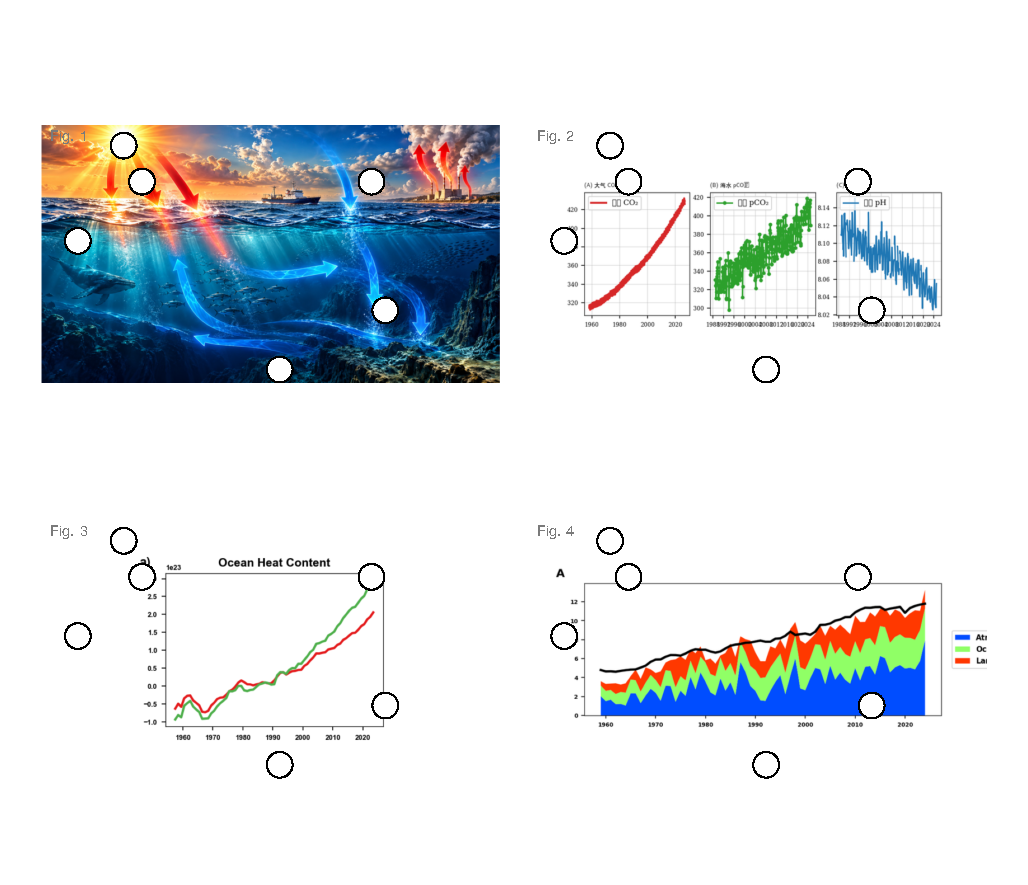
\includegraphics[width=\linewidth]{figures/ch04/ch04-01-inconsistent-set-zh.pdf}
\caption{四张各自看来都还可以的图，放在一起却不成一套（故意不一致的示范）。图中存在六类冲突：（1）红色在四张图中分别表示太阳辐射与工厂排放（Fig.\ 1）、大气 $\text{CO}_2$（Fig.\ 2）、$0\text{--}700\ \text{m}$ 海洋热含量（Fig.\ 3）和陆地碳汇（Fig.\ 4）；（2）示意图中同色箭头兼表不同过程；（3）Fig.\ 3 仅靠红绿区分两条线且未标图例；（4）Fig.\ 4 用彩虹色图绘制堆叠面积，右侧图例被裁切；（5）四图混用三种字体与四种面板编号写法，且因字体未统一配置，子图标题与标记圆圈中的上下标或序号出现缺字方框与空白圆圈；（6）示意图采用立体光泽画风，并混入太阳、轮船、鲸、鱼群等正文未讨论的对象。Fig.\ 2–4 使用真实公开数据，仅改变了样式。}\label{fig:ch04-01}
\end{figure}

顺着读者的视线在图~\ref{fig:ch04-01} 的四个象限间扫视，就能体会读图的阻力：左上角 Fig.\ 1 中，发光红箭头既从太阳射向海面（热量输入），又从工厂烟囱升向天空（人为碳排放）；右上角 Fig.\ 2 中，红线代表大气 $\text{CO}_2$；左下角 Fig.\ 3 中，红线变成 $0\text{--}700\ \text{m}$ 海洋热含量；右下角 Fig.\ 4 中，顶层红色色块又变成陆地碳汇。绿色在 Fig.\ 2b、Fig.\ 3、Fig.\ 4 中分别代表海水 $p\text{CO}_2$、$0\text{--}2000\ \text{m}$ 热含量和海洋碳汇；蓝色在 Fig.\ 1、Fig.\ 2c、Fig.\ 4 中分别代表海气交换与环流、海水 pH 和大气碳增长。读者每翻过一张图，都得强行忘掉上一张图的颜色含义，重新寻找图例解码（表~\ref{tab:ch04-diag}）。

\begin{table}[htbp]\centering\footnotesize
\setlength{\tabcolsep}{3pt}
\renewcommand{\arraystretch}{1.15}
\caption{不一致初稿（图~\ref{fig:ch04-01}）的逐项诊断及其给读者造成的理解代价。}\label{tab:ch04-diag}
\begin{tabularx}{\linewidth}{@{}Y>{\raggedright\arraybackslash}p{18mm}Y@{}}
\toprule
\textbf{初稿中出现的视觉冲突} & \textbf{出现位置} & \textbf{读者付出的理解代价} \\
\midrule
红、绿、蓝三色跨图含义冲突（如红色在四图中分别代表热与排放、大气 $\text{CO}_2$、上层热含量、陆地碳汇） & Fig.\ 1–4 & 读者在图间来回对照时，误把同一颜色当成同一个物理量或碳库 \\
示意图中蓝色箭头既表示水体环流又表示海气碳交换，红色箭头既表示太阳热辐射又表示烟囱碳排放 & Fig.\ 1 & 无法从箭头的几何外观判断所代表的过程类型 \\
仅靠纯红与纯绿区分两条等粗曲线，且图面未标图例或直接标注 & Fig.\ 3 & 红绿色觉差异读者无法分辨 $0\text{--}700\ \text{m}$ 与 $0\text{--}2000\ \text{m}$ 深度层 \\
采用 \texttt{jet} 彩虹色图绘制三层碳汇堆叠面积，且因未画收支不平衡项导致堆叠顶缘穿越总排放黑线 & Fig.\ 4 & 颜色顺序无物理意义，明度跳跃制造假边界，且造成“分项之和大于总排放”的误读 \\
混用三种字体与四种面板编号格式（\texttt{(A)}、\texttt{a)}、\texttt{A}、无编号），上下标与圆圈序号出现缺字方框 & Fig.\ 1–4 & 版面显得临时拼凑；正文引用“图 3a”或“图 2b”时读者难以快速定位 \\
字号从 $6\ \text{pt}$ 到 $12\ \text{pt}$ 不等，图内标题与下方图注重复，右侧图例框超出画布被裁切 & Fig.\ 2–4 & 视觉层级混乱，挤占数据展示面积，且产生残缺文字 \\
3D 立体光泽示意图与二维扁平数据图风格割裂，示意图中加入太阳、轮船、鲸和鱼群 & Fig.\ 1 & 暗示正文并未讨论的短波辐射或生态航次过程，视觉重心落在装饰物上 \\
纵轴单位记法不一，Fig.\ 3 因重复乘上量级因子触发顶端“\texttt{1e23}”科学计数偏移且无单位名称 & Fig.\ 2–4 & 读者需要停下来重新换算数量级与物理量纲 \\
\bottomrule
\end{tabularx}
\end{table}

一篇论文的所有配图不是孤立插画，而是一套协同论证的视觉系统。当多个面板反复讨论同一批物理量或碳库时，颜色、字号、线型、箭头和图标就构成了整篇论文的\textbf{视觉语言}。本章讨论如何在动手出图前立下一页视觉规范，将其转化为可粘贴进 \scidraw{} 的风格约束与核验清单，让全篇配图讲同一种语言。

\section{颜色先有含义，再有好看}

许多研究者配色时首先关心“哪套色板更好看”。但在科研论文中，颜色的首要职责不是装饰，而是\textbf{承载语义}。读者会本能地把同一种醒目颜色当成同一研究对象或同一类物理量（Wong, 2010；Krzywinski, 2013）。若颜色只按单张图的作图顺序随意分配，跨图对照的线索就会断裂。

\textbf{第一，按科学含义分配“语义色”，并在全文锁定。}建立视觉语言的第一步，是列出全文所有图表中反复出现的核心物理量或角色，为每个角色指定专属色值（语义色），明确规定它“用于什么”和“绝不用于什么”。在小宋的论文中，全文锁定六个定量角色与一个示意图专用角色：
\begin{itemize}
\item \textbf{大气碳（$\text{CO}_2$）：}橙色（\texttt{\#E69F00}），用于 Fig.\ 1 大气 $\text{CO}_2$ 分子点、Fig.\ 2a 大气 $\text{CO}_2$ 曲线和 Fig.\ 4a 大气碳增长，不用于热量或海洋量。
\item \textbf{海洋碳：}蓝色（\texttt{\#0072B2}），用于 Fig.\ 1 表层海水溶解无机碳（DIC）、Fig.\ 2b 海水 $p\text{CO}_2$、Fig.\ 4a 海洋碳汇及 Fig.\ 4b 海洋碳汇占比，不用于水体背景或温度。
\item \textbf{陆地碳：}蓝绿色（\texttt{\#009E73}），仅用于 Fig.\ 4a 陆地碳汇，不用于示意图中的浮游植物图标。
\item \textbf{热量：}朱红色（\texttt{\#D55E00}），用于 Fig.\ 1 热通量箭头和 Fig.\ 3 海洋热含量曲线，不用于任何碳量。
\item \textbf{海水 pH：}红紫色（\texttt{\#CC79A7}），专用于 Fig.\ 2c 表层海水 pH。
\item \textbf{人为排放与碳输入通量：}近黑深灰（\texttt{\#3C3C3C}），用于 Fig.\ 4a 总排放曲线及 Fig.\ 1 碳通量方向箭头。
\item \textbf{水体输运（仅示意图）：}天蓝色（\texttt{\#56B4E9}）半透明宽带，专用于 Fig.\ 1 携热与碳下沉的环流带，不作数据图折线。
\end{itemize}

\textbf{第二，控制语义色总数，用同色相的不同明度区分同类变体。}人眼在同一视野内无需反复查表即可记住的颜色类别很有限，全文语义色不宜超过 6 至 7 个（Wong, 2010）。坐标轴、参考线、背景分区和示意图标本体一律退居中性灰（\texttt{\#F2F2F2}、\texttt{\#BDBDBD}、\texttt{\#7A7A7A}）。当同一面板需比较同一物理量的两个变体——如 Fig.\ 3 同时展示 $0\text{--}700\ \text{m}$ 与 $0\text{--}2000\ \text{m}$ 海洋热含量距平——不应借用代表碳汇的绿或蓝，而应\textbf{保持“热量 = 朱红（\texttt{\#D55E00}）”的色相不变，用深浅明度区分深度}：$0\text{--}2000\ \text{m}$ 用全饱和度深朱红（\texttt{\#D55E00}），$0\text{--}700\ \text{m}$ 用向白色混合 $45\%$ 的浅朱红（保留 $55\%$ 原色强度），并在曲线右端直接标出深度（图~\ref{fig:ch04-02}、图~\ref{fig:ch04-03}）。读者一眼便知两条线都代表海洋热量，又能清晰分辨深浅两层。

\begin{figure}[htbp]\centering
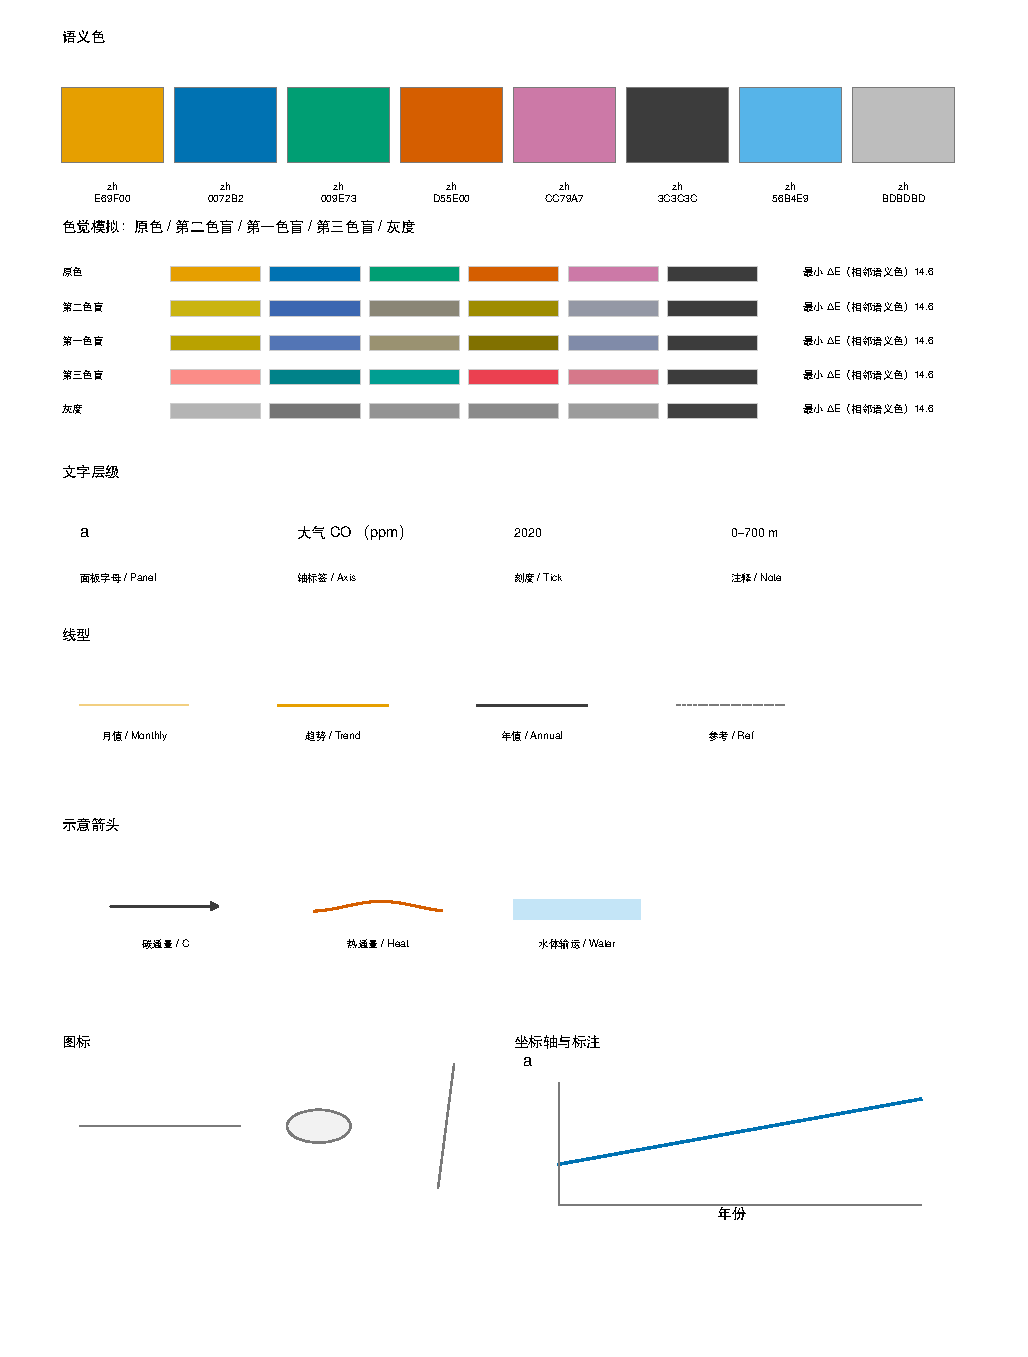
\includegraphics[width=0.95\linewidth,height=0.80\textheight,keepaspectratio]{figures/ch04/ch04-02-spec-page-zh.pdf}
\caption{本案例论文的一页视觉规范（v1）。自上而下规定语义色色板、三种色觉差异模拟与灰度检查、最终印刷尺寸下的四级文字层级、数据图线型、示意图过程箭头、中性图标风格及坐标轴布局。色觉模拟行右侧数值（$14.6$）为同面板相邻语义色间的最小感知色差（CAM02-UCS $\Delta E$），由脚本计算。}\label{fig:ch04-02}
\end{figure}

\textbf{第三，以无障碍色板为起点，绝不单靠红绿区分。}欧洲血统人群中约 $8\%$ 的男性存在先天性红绿色觉差异，其中以第二色觉异常（deuteranomaly，绿色弱/盲）最常见（Wong, 2011；注意该文于 2023 年发表了作者更正，修正了原文视锥细胞光谱曲线标注与部分术语）。图~\ref{fig:ch04-01} 中 Fig.\ 3 纯靠鲜红（\texttt{\#E41A1C}）与鲜绿（\texttt{\#4DAF4A}）区分的两条等粗曲线，在第二色盲模拟下会变成两条难以分辨的暗黄褐色线（图~\ref{fig:ch04-03} 上行右列）。因此，选色应以经过色觉通用设计验证的 Okabe–Ito 色板（Okabe 与 Ito, 2008；Wong, 2011）或 ColorBrewer 方案（Brewer）为起点。

\begin{figure}[htbp]\centering
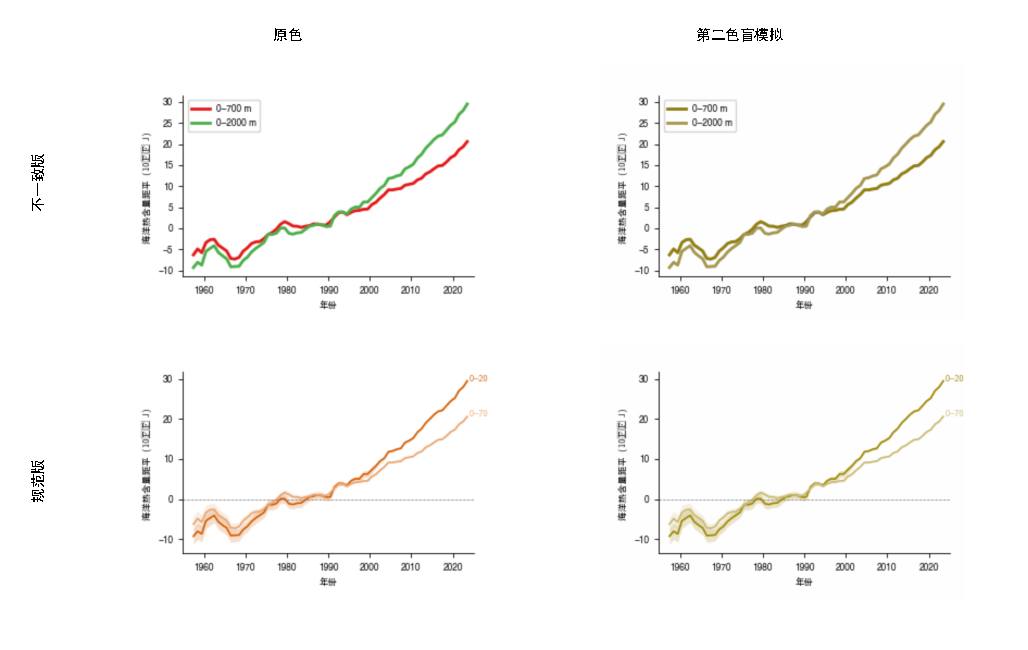
\includegraphics[width=\linewidth]{figures/ch04/ch04-03-cvd-check-zh.pdf}
\caption{只靠红绿区分的两条线，在第二色盲模拟下难以分辨（上）；同一色相的两种明度加直接标注，在模拟下仍可区分（下）。右列为对整幅渲染图像像素执行的第二色盲模拟（\texttt{colorspacious}，deuteranomaly，严重度 $100$）。数据：NOAA NCEI 全球海洋热含量五年平均距平（Levitus 等, 2012）。}\label{fig:ch04-03}
\end{figure}

\textbf{第四，结合色觉模拟与灰度检查，叠加冗余编码。}即便选用 Okabe–Ito 色板，多色同框时仍需定量核验。图~\ref{fig:ch04-02} 第二部分展示了各语义色在原色、第二色盲、第一色盲（protanomaly）、第三色盲（tritanomaly，严重度均为 $100$）及 CIELAB 明度灰度（$L^*$）下的外观，并计算同面板相邻语义色在 CAM02-UCS 空间中的最小色差 $\Delta E$。本书给出一条操作建议（属于实用自查参考值，非强制标准）：\textbf{同面板相邻颜色在色觉模拟下的 CAM02-UCS 色差宜满足 $\Delta E \ge 15$，转灰度后的明度差宜满足 $\Delta L^* \ge 15$；若不足，则必须叠加形状、线型或线端直接标注作为冗余。}

图~\ref{fig:ch04-02} 中相邻语义色的最小 $\Delta E$ 实测值为 $14.6$，刚巧擦过 $15$ 的参考线边缘，且灰度行中蓝、蓝绿与朱红的明度颇为接近。这说明任何多色色板都不能单靠色相硬扛。如图~\ref{fig:ch04-03} 下行所示，改用深浅朱红配标准误阴影带与右端直接标注后，即使在严重度 $100$ 的第二色盲模拟下依然清晰可辨。同时需注意，数值模拟只是色度学近似，定稿前打印黑白稿自查并请有色觉差异的同行看一眼，不能省略。

\textbf{第五，连续变量用感知均匀色图，告别彩虹色图。}映射二维连续场或多项堆叠时，禁用 \texttt{jet} 等彩虹色图。Crameri 等（2020）指出，彩虹色图明度随数值变化不单调，在青、黄区制造虚假边界且对色觉差异读者不友好。连续单向变量应选 \texttt{viridis} 或 \texttt{cividis}（Nuñez 等, 2018）等感知均匀顺序色图；正负距平应以零值为中心选用双端发散色图。

\section{文字层级按最终尺寸定}

图~\ref{fig:ch04-01} 显得拼凑的另一原因是文字失控：Fig.\ 2 用衬线体 \texttt{DejaVu Serif}（$11\ \text{pt}$）、编号“\texttt{(A)(B)(C)}”；Fig.\ 3 用 \texttt{Arial} 粗体（$9\ \text{pt}$）、编号“\texttt{a)}”；Fig.\ 4 用 \texttt{DejaVu Sans}（$8\ \text{pt}$）、编号“\texttt{A}”。各图画布尺寸不一，缩进论文版心后字号忽大忽小。

\textbf{第一，先锁定期刊最终印刷尺寸，再定字号。}若在脚本里随手设 $10 \times 6$ 英寸（约 $254 \times 152\ \text{mm}$），缩进单栏宽 $85\ \text{mm}$ 时字号会缩至三分之一，$10\ \text{pt}$ 刻度变成难以辨认的 $3.3\ \text{pt}$（Rougier 等, 2014；Wong, 2011 Typography）。正确顺序是先按目标期刊《作者指南》设定画布物理宽度——单栏图通常宽 $85\text{--}89\ \text{mm}$，双栏通栏图通常宽 $174\text{--}183\ \text{mm}$（本案例 Fig.\ 1、2、4 设为 $174\ \text{mm}$，Fig.\ 3 设为 $85\ \text{mm}$）——再按目标点数设定字号，并在 $100\%$ 打印比例下核对。

\textbf{第二，建立四级文字层级，全文统一无衬线字体。}图面文字靠字号与字重分为四级（图~\ref{fig:ch04-02}“文字层级”区）：
\begin{enumerate}
\item \textbf{面板字母（8 pt 粗体）：}小写粗体 \textbf{a}、\textbf{b}、\textbf{c}，不加括号，置于坐标轴框左上外侧。
\item \textbf{坐标轴标签（7 pt 常规）：}“物理量名称（单位）”，如“大气 $\text{CO}_2$（ppm）”。
\item \textbf{刻度数字（6 pt 常规）：}水平排列，不旋转、不重叠。
\item \textbf{图内注释与示意标签（6–7 pt 常规）：}曲线末端直接标注及状态注记用 $6\ \text{pt}$（曲线标注与曲线同色）；示意图叠加标签中，分区与主要对象用 $7\ \text{pt}$，过程名称用 $6\ \text{pt}$。
\end{enumerate}

英文版全文统一用无衬线体（\texttt{Helvetica}、\texttt{Arial} 或 \texttt{TeX Gyre Heros}），在小字号下笔画均匀清晰（Wong, 2011 Typography）。中文版汉字用等线/黑体（如 \texttt{FandolHei} 或思源黑体），但数字、拉丁字母与单位仍用西文无衬线字体。

这里要警惕一个实测字体陷阱：观察图~\ref{fig:ch04-01} 右上 Fig.\ 2、图~\ref{fig:ch04-02} 文字示例以及后文图~\ref{fig:ch04-05}、图~\ref{fig:ch04-07} 的纵轴标签可见，当脚本把 Unicode 下标 $2$、上标负号或带圈序号直接混在中文字符串里交给黑体渲染时，由于中文字库缺少这些专用字形，PNG 栅格图中出现了缺字方框，而在走 PGF/XeLaTeX 的 PDF 中缺字被静默丢弃——导致“大气 $\text{CO}_2$”变成“大气 CO”、“$\text{GtC yr}^{-1}$”变成“$\text{GtC yr}^{1}$”，图~\ref{fig:ch04-02} 色块上方也因脚本元组索引错位印出了语言代码“\texttt{zh}”。因此，混排中英文与上下标时不能依赖字体自动回退，应使用规范的数学/上下标语法（如 \texttt{\textbackslash textsubscript\{2\}}），并在导出 PDF 后放大到 $200\%$ 逐字检查。

\textbf{第三，统一单位记法，用直接标注取代图例框，删去图内标题。}图~\ref{fig:ch04-01} 的 Fig.\ 3 因把已按 $10^{22}\ \text{J}$ 计的数值又乘上 $10^{22}$，触发了纵轴顶端的科学计数偏移“\texttt{1e23}”，且无轴名称。规范做法是全文统一括号内 SI 单位（$10^{22}\ \text{J}$、$\text{GtC yr}^{-1}$、$\mu\text{atm}$、ppm）；删去与图注重复的图内标题；省去图例框，直接把序列名称用同色文字标在曲线右端（Wong, 2011 Typography）。

\section{线型与箭头只说一件事}

在不一致初稿（图~\ref{fig:ch04-01}）中，几何线条同样混乱：Fig.\ 2a 把月均值与去季节趋势画成两条等粗（$2\ \text{pt}$）红线叠成粗带；Fig.\ 2b 用绿实线把离散航次采样点连成折线；Fig.\ 1 示意图用同一种发光粗箭头兼表气体交换、辐射传热和大洋环流。核心原则只有一条：\textbf{同一含义只用一种画法，同一画法只代表一种含义。}

数据图中，不同统计性质或采样频率的数据序列通过线宽、透明度和点线形式严格区分（表~\ref{tab:ch04-lines}）：

\begin{table}[htbp]\centering\footnotesize
\setlength{\tabcolsep}{4pt}
\renewcommand{\arraystretch}{1.15}
\caption{本案例数据图的线型与点型规范（对应视觉规范 C 节）。}\label{tab:ch04-lines}
\begin{tabularx}{\linewidth}{@{}>{\raggedright\arraybackslash}p{36mm}Y>{\raggedright\arraybackslash}p{42mm}@{}}
\toprule
\textbf{数据序列性质} & \textbf{规定画法} & \textbf{本案例应用面板} \\
\midrule
高频原始观测（月均值） & $0.5\ \text{pt}$ 细实线，序列语义色向白色混合 $50\%$ 后的浅色 & Fig.\ 2a 莫纳罗亚大气 $\text{CO}_2$ 月均值 \\
去季节 / 滑动平均趋势 & $1.2\ \text{pt}$ 粗实线，全饱和度语义色 & Fig.\ 2a 去季节值、Fig.\ 3 热含量、Fig.\ 4b 滑动平均 \\
离散航次或非连续采样 & 直径 $2.5\ \text{pt}$ 实心圆点，\textbf{不加连线} & Fig.\ 2b 海水 $p\text{CO}_2$、Fig.\ 2c pH、Fig.\ 4b 年比值 \\
年度收支时间序列 & $1.0\ \text{pt}$ 实线，对应语义色 & Fig.\ 4a 排放与三大碳汇年值 \\
不确定性区间（标准误等） & 同色 $20\%$ 不透明度填充带，无边线 & Fig.\ 3（$\pm 1\ \text{WOse}$）、Fig.\ 4a（平均误差带） \\
参考线与站点变更标记 & $0.5\ \text{pt}$ 中深灰（\texttt{\#7A7A7A}）细虚线，配 $6\ \text{pt}$ 灰字注记 & Fig.\ 2a 换站竖线、Fig.\ 3 零距平水平线 \\
\bottomrule
\end{tabularx}
\end{table}

例如，莫纳罗亚月均值来自连续日观测汇总，用 $0.5\ \text{pt}$ 浅橙细线衬底、叠 $1.2\ \text{pt}$ 鲜橙去季节粗线，既保留季节振幅又突出长期趋势；而夏威夷海洋时间序列（HOT）ALOHA 站数据来自离散出海航次（间隔不均且偶有缺测），若用直线相连就暗示航次之间呈线性变化，因此必须画成无连线圆点。

在概念示意图（Fig.\ 1）中，我们也按“一义一形”为四类物理与生物地球化学过程规定了互不重叠的箭头几何形态（表~\ref{tab:ch04-arrows}）：

\begin{table}[htbp]\centering\footnotesize
\setlength{\tabcolsep}{4pt}
\renewcommand{\arraystretch}{1.15}
\caption{本案例示意图的过程箭头规范（对应视觉规范 D 节）。}\label{tab:ch04-arrows}
\begin{tabularx}{\linewidth}{@{}>{\raggedright\arraybackslash}p{36mm}Y>{\raggedright\arraybackslash}p{44mm}@{}}
\toprule
\textbf{物理 / 生物地球化学过程} & \textbf{规定几何形态与颜色} & \textbf{形状与颜色双重冗余作用} \\
\midrule
碳通量（人为排放、海气交换） & 直线、实心三角头，近黑深灰（\texttt{\#3C3C3C}），$1.0\ \text{pt}$ & 与热通量既靠“深灰对朱红”区分，又靠“直线实心头对波浪开口头”区分 \\
热通量（海气热量吸收与下传） & 波浪线、开口 V 形头，朱红色（\texttt{\#D55E00}），$1.0\ \text{pt}$ & 借用传热学波浪线惯例，黑白打印或色盲视图下仍可凭形状认出 \\
水体下沉与大洋内部输运 & 宽 $4\text{--}6\ \text{pt}$ 天蓝（\texttt{\#56B4E9}）半透明流带，内嵌顺流向人字纹 & 用面状宽带代表大尺度水团运动，与代表界面通量的细线箭头分开 \\
下沉有机颗粒（生物泵输出） & 点线、小实心三角头，近黑深灰（\texttt{\#3C3C3C}），$0.8\ \text{pt}$ & 用离散点线呼应颗粒沉降，线宽细于海气交换主箭头以体现次级角色 \\
\bottomrule
\end{tabularx}
\end{table}

每种箭头在示意图底部图例中定义一次，即使黑白打印，直线、波浪线、人字纹宽带和细点线也绝不会混淆。

\section{图标与示意元素的风格}

在同时包含示意图与数据图的论文里，常见毛病是数据图扁平克制，Fig.\ 1 却是带镜头光晕、水面焦散和立体阴影的 3D 渲染画（图~\ref{fig:ch04-04} 左）。要让示意图融入全文视觉语言，需遵守五条规则（规范 E 节）：

\textbf{第一，图标本体用中性色填充，把语义色留给被追踪的“量”。}工厂烟囱和浮游植物细胞只是过程载体。若把浮游植物涂成绿色，读者就会联想到 Fig.\ 4 的“陆地碳汇（\texttt{\#009E73}）”。因此图标本体一律用浅灰或中灰填充（\texttt{\#F2F2F2}、\texttt{\#BDBDBD}），只让大气 $\text{CO}_2$ 圆点用橙色、表层海水 DIC 圆点用蓝色、热通量箭头用朱红、水体输运带用天蓝；背景水层仅用极低饱和度的浅蓝灰（表层混合层 \texttt{\#DCEBF5}、海洋内部 \texttt{\#C9DEEE}）做结构分层。

\textbf{第二，描边粗细与数据图坐标轴对齐。}数据图坐标轴为 $0.6\ \text{pt}$，示意图标轮廓与海面分界线统一设为接近的 $0.75\ \text{pt}$ 深灰（\texttt{\#3C3C3C}）圆角描边。

\textbf{第三，采用二维简化轮廓，去掉渐变、阴影、高光与写实水纹。}留出干净背景安放文字标签。

\textbf{第四，同一对象在不同图中画法一致。}如海面波线与混合层分界在各处保持相同轮廓。

\textbf{第五，不画未讨论的装饰对象，守住机制表述的科学边界。}图~\ref{fig:ch04-04} 左图画了烈日与直射光束（暗示研究短波辐射）、科考船（暗示特定航次观测），模型还自行生成了鲸、鱼群与海底礁石。这些无关元素会误导读者对研究范围的判断。

\begin{figure}[htbp]\centering
\begin{minipage}[c]{0.48\linewidth}\centering
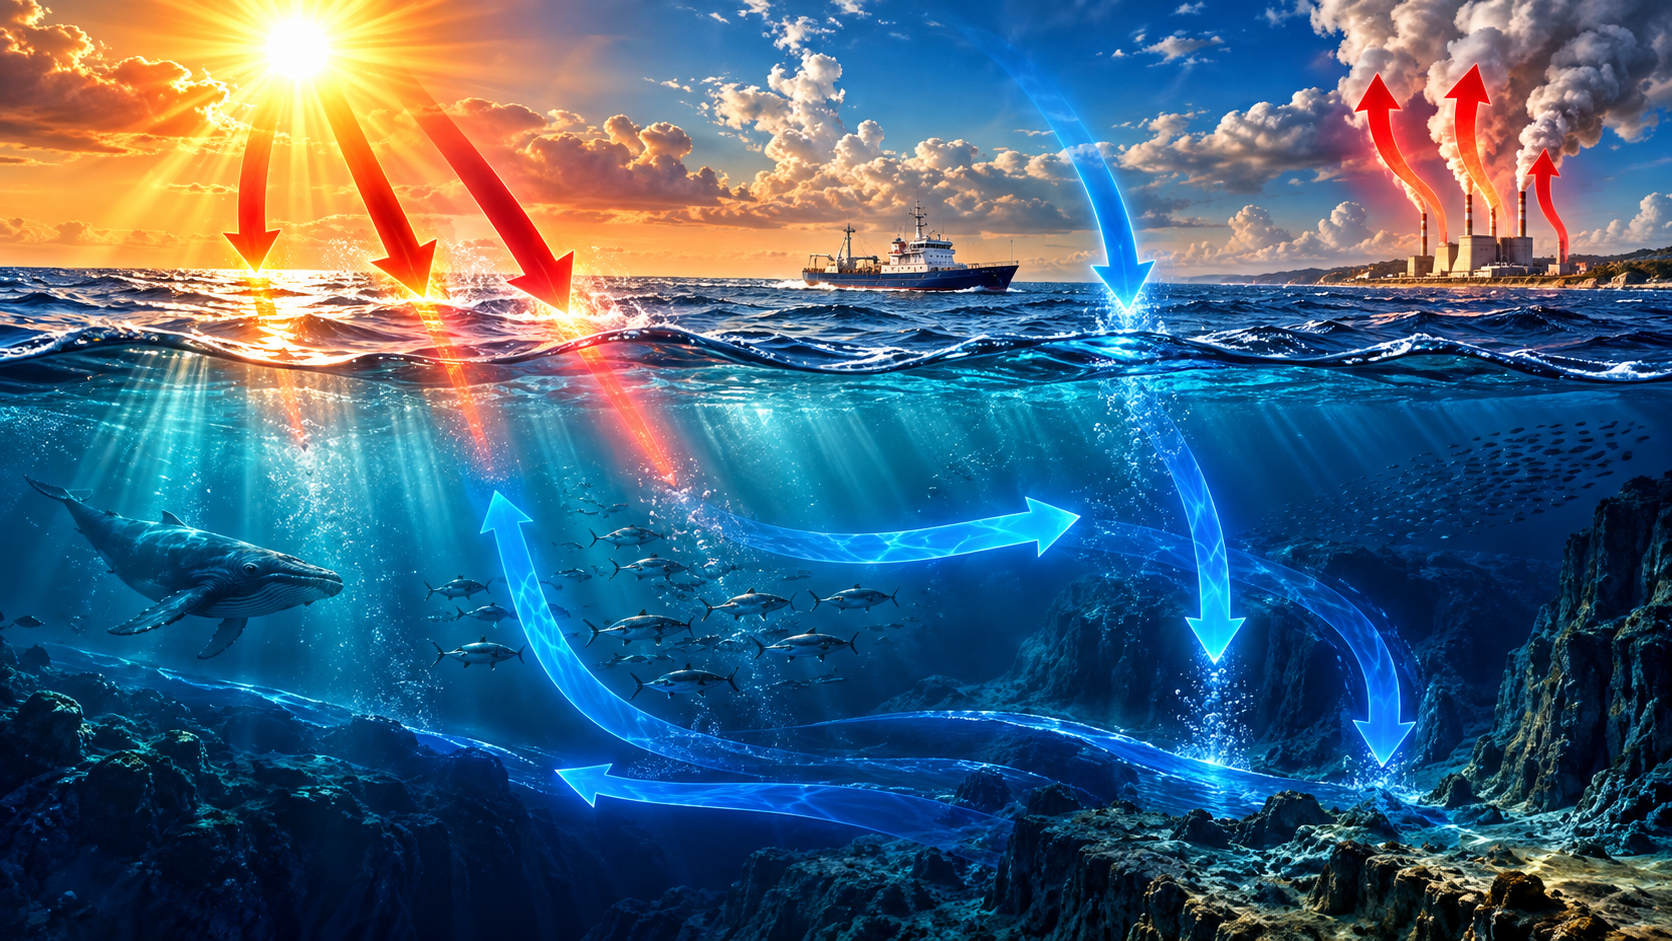
\includegraphics[width=\linewidth]{figures/ch04/ch04-04a-schematic-bad.png}
\end{minipage}\hfill
\begin{minipage}[c]{0.48\linewidth}\centering
\resizebox{\linewidth}{!}{\hbox{\setlength{\linewidth}{\textwidth}% FIG ch04-04b schematic labels (Chinese)
\usetikzlibrary{positioning}
\begin{tikzpicture}
\node[anchor=south west,inner sep=0] (img) at (0,0) {%
  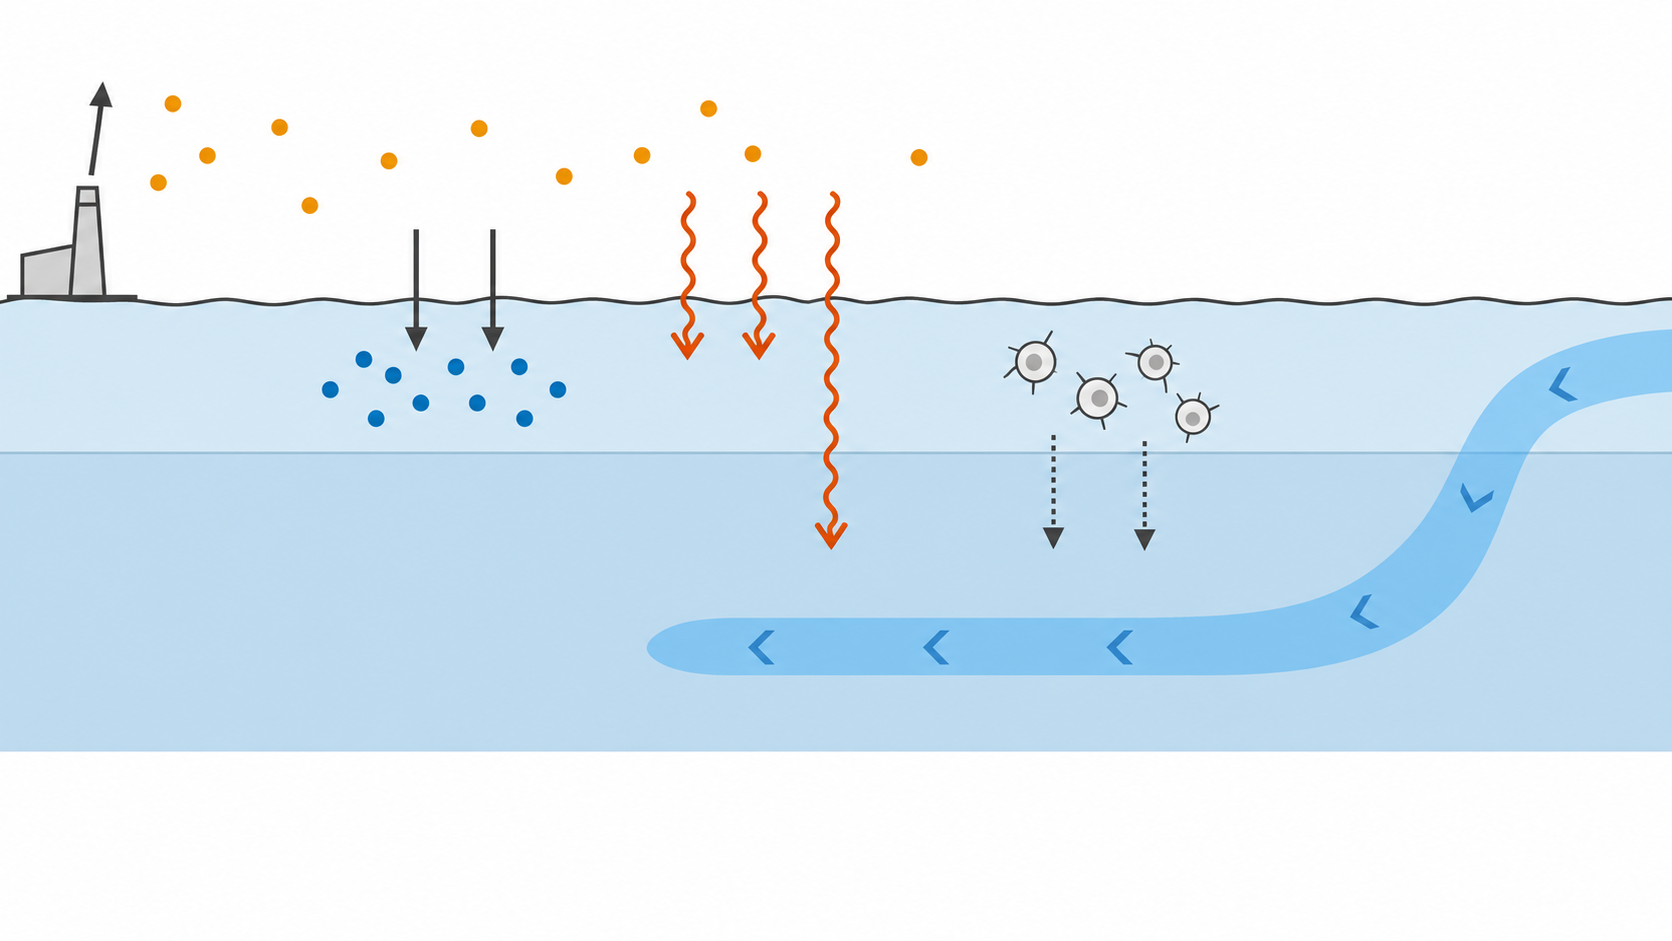
\includegraphics[width=\linewidth]{figures/ch04/ch04-04b-schematic-base.png}};
\begin{scope}[x={(img.south east)},y={(img.north west)},font=\sffamily\small]
  \node at (0.92,0.90) {大气};
  \node at (0.92,0.66) {表层混合层};
  \node at (0.92,0.35) {海洋内部};
  \node[align=left] at (0.06,0.93) {人为排放};
  \node at (0.30,0.88) {CO\textsubscript{2}};
  \node at (0.33,0.70) {海气交换};
  \node at (0.30,0.60) {溶解无机碳};
  \node at (0.55,0.70) {热量吸收};
  \node[align=center] at (0.80,0.45) {水体下沉\\与输运};
  \node at (0.48,0.62) {浮游植物};
  \node[align=center] at (0.48,0.42) {下沉颗粒\\（生物泵）};
  \node[align=center,font=\scriptsize] at (0.50,0.04) {%
    图例：碳通量 / 热通量 / 水体输运 / 下沉颗粒};
\end{scope}
\end{tikzpicture}
}}
\end{minipage}
\caption{示意图也服从同一套视觉语言。左（故意不一致的示范）：3D 光泽渲染、装饰性太阳与船只、模型自行添加的鲸与鱼群，且同色箭头兼表不同过程。右：按规范重画的无文字底图叠加 TikZ 标签，颜色严格留给大气 $\text{CO}_2$（橙）、海水溶解无机碳（蓝）、热（朱红）和水体输运（天蓝），四类过程各用一种箭头形状。两图均为图像模型生成的示意，不按比例。}\label{fig:ch04-04}
\end{figure}

同时要注意右图中“生物泵”的科学边界：浮游植物固碳并以沉降颗粒向深海输出的生物泵，主要转运自然碳循环中的碳；工业革命以来海洋对\textbf{人为 $\text{CO}_2$} 的净吸收，主要由海气气体交换、碳酸盐缓冲化学与物理环流决定（Sabine 等, 2004；Gruber 等, 2019；Fox-Kemper 等, 2023；Canadell 等, 2023）。因此右图将人为 $\text{CO}_2$ 海气交换（左中部深灰实线箭头 $\rightarrow$ 蓝色 DIC 圆点 $\rightarrow$ 右侧天蓝水体下沉带）作为主路径，而将浮游植物与细点线颗粒箭头独立置于中右部，避免画成“人为碳靠浮游植物送入深海”的错误单线链路。

\section{用提示词约束风格，再逐项检查}

立好规范后，用 AI 工具出图时需认清两个客观事实。第一，\textbf{对话式 AI 在协助起草规范或梳理文献时，不了解细分领域惯例，还可能推荐已撤稿文献}——例如利用大气氧碳推算海洋热吸收的一篇 2018 年 \textit{Nature} 论文（Resplandy 等, 2018）已于 2019 年因误差与趋势方法问题撤稿，故所有引文必须经 Crossref 核查撤稿状态。第二，\textbf{\scidraw{} 目前没有跨会话或项目级的全局风格记忆}，界面上的风格预设也不等于你的论文规范。

因此，可靠做法是先把视觉规范保存为带版本号的文档（图~\ref{fig:ch04-02}），提炼出两段可复制的“风格块（style block）”；每次新开会话时先粘贴风格块，生成或修改后再逐项核验。本案例的一页视觉规范（v1）核心条款摘录如下（完整版见配套资料）：

\begin{BookNote}
\textbf{一页视觉规范（v1）核心条款摘录：}
\begin{itemize}
\item \textbf{A.\ 语义色（基于 Okabe–Ito 色板）：}大气碳 \texttt{\#E69F00}（橙，用于 Fig.\ 2a、Fig.\ 4a 大气增长、示意图大气 $\text{CO}_2$ 点，不用于热或海洋量）；海洋碳 \texttt{\#0072B2}（蓝，用于 Fig.\ 2b 海水 $p\text{CO}_2$、Fig.\ 4 海洋碳汇、示意图海水溶解无机碳，不用于水体背景或热）；陆地碳 \texttt{\#009E73}（蓝绿，仅用于 Fig.\ 4 陆地碳汇，不用于浮游植物图标）；热 \texttt{\#D55E00}（朱红，用于 Fig.\ 3 深浅两线与示意图热通量，不用于碳量）；海水 pH \texttt{\#CC79A7}（红紫，专用于 Fig.\ 2c）；人为排放 \texttt{\#3C3C3C}（近黑深灰）；水体输运 \texttt{\#56B4E9}（天蓝，仅用于示意图环流带）；中性灰 \texttt{\#F2F2F2}、\texttt{\#BDBDBD}、\texttt{\#7A7A7A}（背景分区、图标填充、参考线）。
\item \textbf{B.\ 文字层级与尺寸：}Fig.\ 1、2、4 物理宽 $174\ \text{mm}$（双栏），Fig.\ 3 宽 $85\ \text{mm}$（单栏）。面板字母 $8\ \text{pt}$ 粗体小写 \textbf{a}、\textbf{b}、\textbf{c}（左上外侧）；轴标签 $7\ \text{pt}$ 常规；刻度与线端直接标注 $6\ \text{pt}$ 常规（标注与对象同色）；示意图叠加标签对象 $7\ \text{pt}$、过程 $6\ \text{pt}$。图内不放标题，单位统一为括号内 SI 写法（$10^{22}\ \text{J}$、$\text{GtC yr}^{-1}$、$\mu\text{atm}$、ppm）。
\item \textbf{C–E.\ 线型、箭头与图标：}见表~\ref{tab:ch04-lines} 与表~\ref{tab:ch04-arrows}；图标用 $0.75\ \text{pt}$ \texttt{\#3C3C3C} 圆角描边与中性灰填充，无渐变、阴影与高光，禁画太阳、船只、冰山、鱼群。
\item \textbf{F.\ 布局与导出：}坐标轴仅留左下两边（$0.6\ \text{pt}$，刻度朝外），无网格，线端直接标注取代图例框，面板间距 $4\ \text{mm}$；导出矢量 PDF 与高分辨率 PNG，中英文版坐标尺寸一致。
\end{itemize}
\end{BookNote}

在 \scidraw{} 科学可视化（\sdtool{sci-vis}）中每次新开数据图会话时，先粘贴以下数据图风格块：

\begin{Prompt}
Apply this paper-wide figure style exactly (visual spec v1):
- Colours by meaning, no other hues: atmospheric CO2 #E69F00; ocean carbon
  #0072B2; land carbon #009E73; heat #D55E00; seawater pH #CC79A7;
  emissions #3C3C3C; neutral grays #7A7A7A and #BDBDBD only.
- Monthly values: 0.5 pt line in a 50% lighter tint of the series colour.
  Deseasonalized or smoothed values: 1.2 pt solid line. Discrete cruise samples:
  small dots, no connecting line. Uncertainty: band in the series colour at 20%
  opacity, no edge line. Reference lines: 0.5 pt dashed #7A7A7A.
- Sans-serif font. Axis labels 7 pt, tick labels 6 pt, panel letters 8 pt bold
  lowercase (a, b, c) outside the top-left of each axes.
- No title inside the figure, no grid, no legend box: label each series
  directly at its right end in the series colour.
- Only left and bottom axes, 0.6 pt, ticks pointing outward.
- Final size 174 mm wide x 60 mm high.
Keep every data value unchanged: do not smooth, resample, interpolate or drop
rows unless I ask.
\end{Prompt}

\begin{sloppypar}
在提示词绘图（\sdtool{ai-drawing}）或机制图生成（\sdtool{mechanism-figure-generator}）中制作示意图时，则粘贴以下示意图风格块：
\end{sloppypar}

\begin{Prompt}
Flat 2D scientific schematic of ocean heat and carbon uptake, landscape 16:9,
pure white background. ABSOLUTELY NO TEXT: no letters, no words, no numbers, no
symbols, no labels, no legend, no title.
STYLE (paper-wide visual spec v1): flat vector illustration; all outlines 0.75 pt
dark gray #3C3C3C with rounded joins; no gradients, no shadows, no highlights,
no 3D, no glow, no texture, no realistic water. Icons use neutral fills only
(#F2F2F2, #BDBDBD). Colour is used ONLY for the following quantities:
orange #E69F00 = CO2 in the atmosphere; blue #0072B2 = dissolved inorganic
carbon in seawater; vermilion #D55E00 = heat; sky blue #56B4E9 = water
transport. Nothing else may use these colours.
REGIONS (top to bottom): Top 25% atmosphere, white; thin dark gray gently wavy
line at 25% height (sea surface); 25-45% surface mixed layer (#DCEBF5); 45-90%
ocean interior (#C9DEEE); bottom 10% empty white reserved for a legend.
DO NOT DRAW: sun, rays, clouds, ships, fish, ice, land masses other than the
short ground line, sea floor details, coral, bubbles, any charts or data.
\end{Prompt}

\begin{sloppypar}
使用 \sdtool{sci-vis} 时需注意两点：第一，上传数据后的完整性校验（核对哈希、字节数与行数）只证明输入文件未丢行损坏，不证明单位、标度、基准期或配色正确；第二，多轮对话修改极易发生\textbf{风格漂移}——例如追加一句“在 2022 年 12 月加一条细竖线”，工具重写代码时可能悄悄把刻度字号退回默认值或重新加回图例框。因此每次修改后都要复查色值、字号与线型，必要时用历史版本功能回退并重贴风格块。定稿前可用图片检查工具（\sdtool{figure-checker}）筛查分辨率、灰度与色觉风险，但技术检查不代替科学审核。
\end{sloppypar}

\section{案例：四张图从各自为政到一套}

下面回到小宋的论文，按“材料清点 $\rightarrow$ 规范制定 $\rightarrow$ 示意图与数据图重绘 $\rightarrow$ 整套对照与核验”走完整个改造过程。

\textbf{第一步：清点原始材料与数据处理规则。}四套公开数据集于 2026 年 10 月 29 日下载固化，字段、单位、质控规则与引用要求汇总于表~\ref{tab:ch04-sources}。在图 2 中，莫纳罗亚大气 $\text{CO}_2$ 为\textbf{干空气摩尔分数}（ppm），而 ALOHA 站表层海水 $p\text{CO}_2$ 为现场温盐下由 DIC 与总碱度计算的\textbf{分压}（$\mu\text{atm}$）；两者数值虽都在 $300\text{--}430$ 附近，但物理量纲不同，不能硬叠在同一纵轴上，故拆为 \textbf{a}、\textbf{b}、\textbf{c} 三个并排面板。

\begin{table}[htbp]\centering\scriptsize
\setlength{\tabcolsep}{2.5pt}
\renewcommand{\arraystretch}{1.12}
\caption{主案例四张图使用的公开数据源、质控规则与引用要求（2026 年 10 月 29 日下载）。}\label{tab:ch04-sources}
\begin{tabularx}{\linewidth}{@{}>{\raggedright\arraybackslash}p{20mm}>{\raggedright\arraybackslash}p{24mm}>{\raggedright\arraybackslash}p{18mm}Y>{\raggedright\arraybackslash}p{26mm}@{}}
\toprule
\textbf{数据集（图）} & \textbf{文件与规模} & \textbf{字段与单位} & \textbf{数据处理与质控规则} & \textbf{许可与引用要求} \\
\midrule
莫纳罗亚大气 $\text{CO}_2$（Fig.\ 2a） & \path{co2_mm_mlo.csv}；823 行（1958-03 至 2026-09） & \texttt{average}、\path{deseasonalized}（ppm） & 跳过 \texttt{\#} 注释行；确认无 $-99.99$ 缺测（均值 $361.44\ \text{ppm}$）；不自行平滑；标出 2022-12 至 2023-07 火山喷发改在 Maunakea 观测 & 美国政府公开数据；同时致谢 NOAA GML 与 Scripps（Keeling） \\
HOT 表层海水碳酸盐（Fig.\ 2b, c） & \path{HOT_surface_CO2.txt}；355 行（1988-10-31 起） & \path{pCO2calc_insitu}（$\mu\text{atm}$）、\path{pHcalc_insitu} & 跳过前 8 行；将 $\le -900$（缺测码 $-999$）置为 \texttt{NaN}，得有效记录各 346 条；两位年份按 1988–2026 解析；pH 标度需核对 \path{HOT_surface_CO2_readme.pdf} 填入图注 & 按文件头引用 Dore 等（2009）；未见显式开放许可，重绘须规范引用 \\
全球海洋热含量距平（Fig.\ 3） & \path{pent_h22-w0-700m.dat} 与 \texttt{2000m.dat}；各 67 行 & \texttt{YEAR}（1957.5–2023.5）、\texttt{WO}、\texttt{WOse}（$10^{22}\ \text{J}$） & 两深度年份行数一致（均值 $3.84$ 与 $5.09\times 10^{22}\ \text{J}$）；阴影画 $\text{WO} \pm 1\ \text{WOse}$；距平基准期需核对 NCEI 说明页后填入图注 & NOAA NCEI 美国政府作品；引用 Levitus 等（2012） \\
全球碳收支 GCB 2025（Fig.\ 4） & \path{GlobalCarbonBudget_v2025.xlsx}；66 行（1959–2024） & 排放与三大碳汇（$\text{GtC yr}^{-1}$） & 读 \texttt{Global Carbon Budget} 表（第 22 行表头）；总排放 = 化石 + 土地利用；绘平均不确定性（海洋 $\pm 0.4$、陆地 $\pm 0.5$）；面板 b 由作者算海洋占比（均值 $27.01\%$）与 10 年滑动平均 & 遵循 Fair Use 声明；引用 Friedlingstein 等（2026）并致谢 GCP \\
\bottomrule
\end{tabularx}
\end{table}

\textbf{第二步：重绘示意图（Fig.\ 1）并核查生成偏差。}为了看清提示词如何直接决定示意图是否合群，先看图~\ref{fig:ch04-04} 左图（不一致反例）所使用的提示词：

\begin{Prompt}
A glossy, highly polished 3D illustration of an ocean cross-section for a
climate science paper, landscape 16:9. Photorealistic blue waves on top, a
bright sun with radiating rays in a gradient orange-to-blue sky, a small ship
on the surface, shiny glass-like water with caustics and depth of field.
Thick glowing red 3D arrows go from the sky into the water and also from a
factory into the sky; thick glowing blue 3D arrows curve through the water and
also go from the air into the water. Dramatic lighting, lens flare, strong
shadows, saturated colors. No text, no letters, no numbers, no labels.
\end{Prompt}

这段追求“3D 光泽、写实波浪、戏剧性光效”的提示词直接造就了左图的三大硬伤：红箭头同时画在工厂烟囱和太阳光束上，蓝箭头同时画在海气界面和深海环流上，且由于未设排除清单，模型顺手在水下塞进了鲸、鱼群和礁石。

相反，重绘右图时，我们在第 4.5 节的示意图风格块之后接上下列七项对象与过程指令（完整提示词见本书仓库 \texttt{cases/} 目录）：

\begin{Prompt}
OBJECTS AND PROCESSES (draw exactly these, nothing else):
1. Top-left: one simple factory chimney icon in neutral gray on a short ground
   line, with one straight dark gray arrow (filled head) rising into the air.
2. Atmosphere: about 12 small orange dots scattered in the left and middle.
3. Air-sea gas exchange: two straight dark gray arrows with filled heads, going
   down from the atmosphere through the sea surface into the mixed layer.
4. Mixed layer: about 10 small blue #0072B2 dots near the two arrows.
5. Heat uptake: three vermilion wavy arrows with open V-shaped heads, going down
   into the mixed layer; the rightmost continues into the ocean interior.
6. Water transport: on the right, one broad semi-transparent sky-blue band from
   the mixed layer curving down into the interior and running leftward, with
   chevron marks pointing along the flow.
7. Biological pump: 3-4 small round phytoplankton cell icons (neutral fill, gray
   outline) in the mixed layer, and two dotted dark gray arrows pointing down.
Leave white space around each process for labels.
\end{Prompt}

同一提示词连续生成三次候选底图后，逐张核验可见：
\begin{itemize}
\item \textbf{第 1 次候选（因流向自相矛盾淘汰）：}主要对象与数量均符合，但右侧天蓝色水体输运宽带内上、中段的人字纹指向右上，底段却指向左，同一流带内流向迎头相撞，故淘汰。
\item \textbf{第 2 次候选（选用为图~\ref{fig:ch04-04} 右图底图）：}七项对象与四类箭头齐备，右侧输运宽带内人字纹一致顺流指向左下与正左，无文字且无太阳、轮船、鱼群等禁止对象。
\item \textbf{第 3 次候选（落选）：}流向一致，但给浮游植物细胞加了未要求的鞭毛状突起，点线箭头偏粗，且第二色盲模拟下朱红热箭头与内部背景的最小亮度对比（$2.17:1$）略低于第 2 次候选（$2.36:1$）。
\end{itemize}

对选用的第 2 次候选底图做像素复查，仍可发现三处真实偏差：（1）\textbf{色值仅近似命中}——各对象 RGB 中位数实测为大气橙点 \texttt{\#ED9106}（规范 \texttt{\#E69F00}）、海水蓝点 \texttt{\#0571BA}（规范 \texttt{\#0072B2}）、热箭头 \texttt{\#DD4E0A}（规范 \texttt{\#D55E00}）、碳箭头 \texttt{\#3F3F40}（规范 \texttt{\#3C3C3C}），全图精确命中指定 HEX 的像素数为零，且水层与图标仍有轻微明暗纹理；（2）\textbf{分区比例与对象位置偏移}——海面、混合层底界与底部留白起点实测约为 $32\%$、$48\%$、$80\%$（规范为 $25\%$、$45\%$、$90\%$），且 4 个浮游植物细胞偏在混合层中右部，导致按预设中央坐标（横坐标 $0.48$）叠加的“浮游植物”标签落在细胞群左侧空白处（图~\ref{fig:ch04-04} 右），定稿前需在 TikZ 层右移校准；（3）\textbf{原生分辨率限制}——在 $174\ \text{mm}$ 宽度下原生有效分辨率约 $244\ \text{ppi}$，且无矢量可编辑线宽。这直观说明生成式底图只是近似遵循规范，后期取色核查与标签位置微调必不可少。

\textbf{第三步：按规范重绘三张数据图（Fig.\ 2–4）。}共享同一视觉规范常数重绘后（修改对照见表~\ref{tab:ch04-revisions}）：

\begin{figure}[htbp]\centering
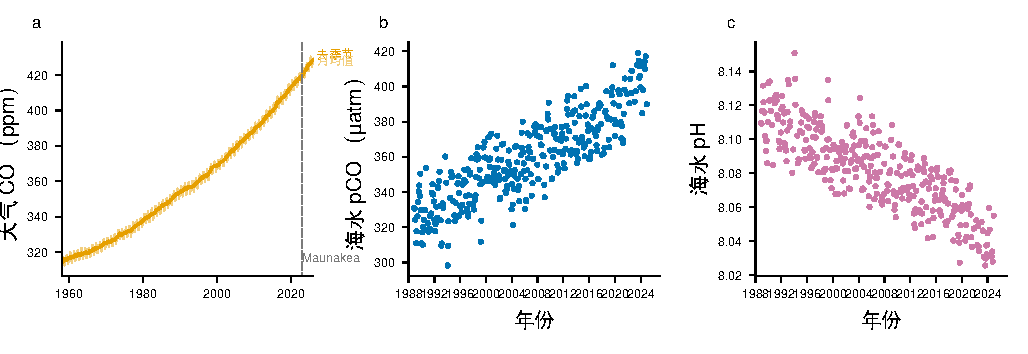
\includegraphics[width=\linewidth]{figures/ch04/ch04-05-fig2-carbonate-zh.pdf}
\caption{按规范重绘的论文 Fig.\ 2：大气 $\text{CO}_2$ 与北太平洋亚热带表层海水碳酸盐系统的变化。（a）莫纳罗亚站大气 $\text{CO}_2$ 月均值（细浅橙线）与去季节值（粗橙线）；1958 年 3 月至 1974 年 4 月数据来自 Scripps，2022 年 12 月至 2023 年 7 月因火山喷发改在 Maunakea 观测（灰色细虚线）。（b）HOT ALOHA 站表层海水 $p\text{CO}_2$（由 DIC 与总碱度计算的现场值，每点一个航次）。（c）同站表层海水 pH（现场温度计算值，标度待核实）。数据：NOAA GML 与 Scripps；HOT（Dore 等, 2009），2026 年 10 月 29 日下载。}\label{fig:ch04-05}
\end{figure}

在图~\ref{fig:ch04-05}（论文 Fig.\ 2）中，面板 \textbf{a} 用橙色（\texttt{\#E69F00}）区分月均值细浅线与去季节粗线，并标出 Maunakea 换站虚线；面板 \textbf{b} 用海洋碳蓝色（\texttt{\#0072B2}）、面板 \textbf{c} 用红紫色（\texttt{\#CC79A7}）将 346 个有效航次画成无连线圆点。$100\%$ 尺寸复查也揭示了三处待微调细节：面板 \textbf{a} 右上末端“去季节”与“月均值”因终值接近而上下重叠，需加纵向偏移；面板 \textbf{b}、\textbf{c} 横轴 4 年间隔刻度略挤，宜改为 10 年一标；纵轴标签下标 $2$ 需补回显式数学下标。

\begin{figure}[htbp]\centering
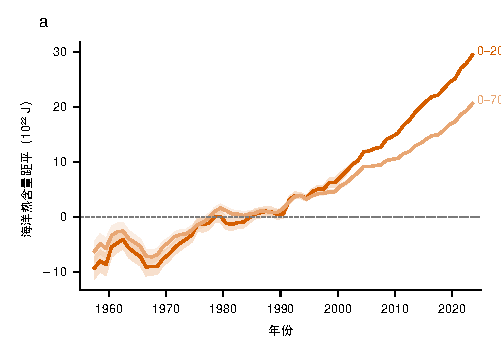
\includegraphics[width=0.58\linewidth]{figures/ch04/ch04-06-fig3-ohc-zh.pdf}
\caption{按规范重绘的论文 Fig.\ 3：全球海洋热含量距平。$0\text{--}700\ \text{m}$（浅朱红）与 $0\text{--}2000\ \text{m}$（深朱红）水层五年平均热含量距平，单位 $10^{22}\ \text{J}$；横轴为五年窗口中点年份；阴影为 NCEI 提供的 $\pm 1$ 标准误；灰虚线为零线。距平基准期需核对 NCEI 文档后注明。数据：NOAA NCEI（Levitus 等, 2012 方法及更新）。}\label{fig:ch04-06}
\end{figure}

在图~\ref{fig:ch04-06}（论文 Fig.\ 3，单栏宽 $85\ \text{mm}$）中，两条曲线统一归入代表热量的朱红色相（\texttt{\#D55E00}），靠深浅明度、$\pm 1\ \text{WOse}$ 阴影带和右端直接标注区分，清晰展现海洋上层与中深层持续吸热的趋势（von Schuckmann 等, 2023）。复查可见右端直接标注“$0\text{--}2000\ \text{m}$”和“$0\text{--}700\ \text{m}$”因右边距预留不足被裁去末尾字符，提示使用线端标注时必须同步放宽横轴上限或右页边距。

\begin{figure}[htbp]\centering
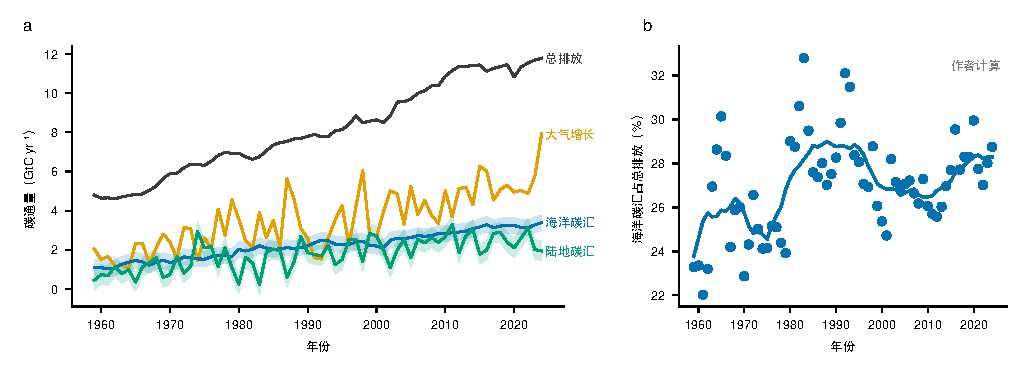
\includegraphics[width=\linewidth]{figures/ch04/ch04-07-fig4-budget-zh.pdf}
\caption{按规范重绘的论文 Fig.\ 4：人为 $\text{CO}_2$ 排放的去向。（a）化石燃料与土地利用变化总排放（深灰）以及大气增长（橙）、海洋碳汇（蓝）、陆地碳汇（蓝绿），单位 $\text{GtC yr}^{-1}$；阴影为 GCB 给出的平均不确定性（海洋 $\pm 0.4$、陆地 $\pm 0.5\ \text{GtC yr}^{-1}$）。（b）海洋碳汇占总排放的比例（作者据 GCB 数据计算；点为年值，线为 10 年居中滑动平均）。收支不平衡项与水泥碳化汇未画出。数据：Global Carbon Budget 2025（Friedlingstein 等, 2026）。}\label{fig:ch04-07}
\end{figure}

在图~\ref{fig:ch04-07}（论文 Fig.\ 4）中，面板 \textbf{a} 将原先因收支不平衡项而穿越黑线的 \texttt{jet} 堆叠面积图改为四条语义色实线配不确定性带，右端同色标签互不重叠；面板 \textbf{b} 用海洋碳蓝色（\texttt{\#0072B2}）画出年值散点与 10 年居中滑动平均线（全期均值约 $27.0\%$），并在右上角注明“作者计算”。

\begin{table}[htbp]\centering\footnotesize
\setlength{\tabcolsep}{3pt}
\renewcommand{\arraystretch}{1.15}
\caption{从不一致初稿（图~\ref{fig:ch04-01}）到规范重绘稿（图~\ref{fig:ch04-04}–\ref{fig:ch04-07}）的修改记录。}\label{tab:ch04-revisions}
\begin{tabularx}{\linewidth}{@{}>{\raggedright\arraybackslash}p{14mm}Y>{\raggedright\arraybackslash}p{20mm}>{\raggedright\arraybackslash}p{36mm}@{}}
\toprule
\textbf{对象图} & \textbf{具体修改内容} & \textbf{依据条款} & \textbf{核对方式与实测复查记录} \\
\midrule
Fig.\ 1 & 删去 3D 光泽、太阳、船只、鲸与鱼群；改为二维分层底图；四类过程按表~\ref{tab:ch04-arrows} 箭头重画；叠加 TikZ 标签 | 规范 A、D、E & 3 次候选中淘汰流向冲突的第 1 次，选第 2 次；记录实测 HEX 近似与浮游植物偏右，待微调标签坐标 \\
Fig.\ 2a & 双红粗线改为 \texttt{\#E69F00} 橙色（月均值 $0.5\ \text{pt}$ 浅线 + 去季节 $1.2\ \text{pt}$ 实线）；补 Maunakea 灰虚线 & 规范 A、C & 取色器核对 HEX；末端两标签轻微重叠，需加纵向偏移 \\
Fig.\ 2b, c & 绿、蓝折线改为 \texttt{\#0072B2}（海洋碳）与 \texttt{\#CC79A7}（pH）的 $2.5\ \text{pt}$ 无连线圆点 & 规范 A、C & 核对 346 个有效航次点无连线；横轴 4 年刻度略挤，宜改为 10 年间隔 \\
Fig.\ 3 & 红绿双线改为朱红（\texttt{\#D55E00}）深浅两色；加 $\pm 1\ \text{WOse}$ 带与零线；去掉 \texttt{1e23} 偏移 & 规范 A、B、C & 第二色盲模拟下可分（图~\ref{fig:ch04-03}）；右端标注被裁半词，需扩右边距 \\
Fig.\ 4 & 彩虹堆叠图改为四条语义色实线 + 误差带；新增面板 b 海洋汇占比并标“作者计算” & 规范 A、B、C & 66 年数值与原表逐年一致；四条线端直接标注清晰 \\
全部四图 & 统一无衬线字体与 8/7/6 pt 层级；面板字母改为左上粗体小写 \textbf{a}–\textbf{c}；删图内标题与网格 & 规范 B、F & 100\% 尺寸 PDF 量字号；排查出上下标字符缺字问题 \\
\bottomrule
\end{tabularx}
\end{table}

\textbf{第四步：整套拼版对照、规范图注与全表核验。}将修改后的四张图按与图~\ref{fig:ch04-01} 相同的 $2 \times 2$ 版式拼成总览（图~\ref{fig:ch04-08}），底部附上六色语义提示条。

\begin{figure}[htbp]\centering
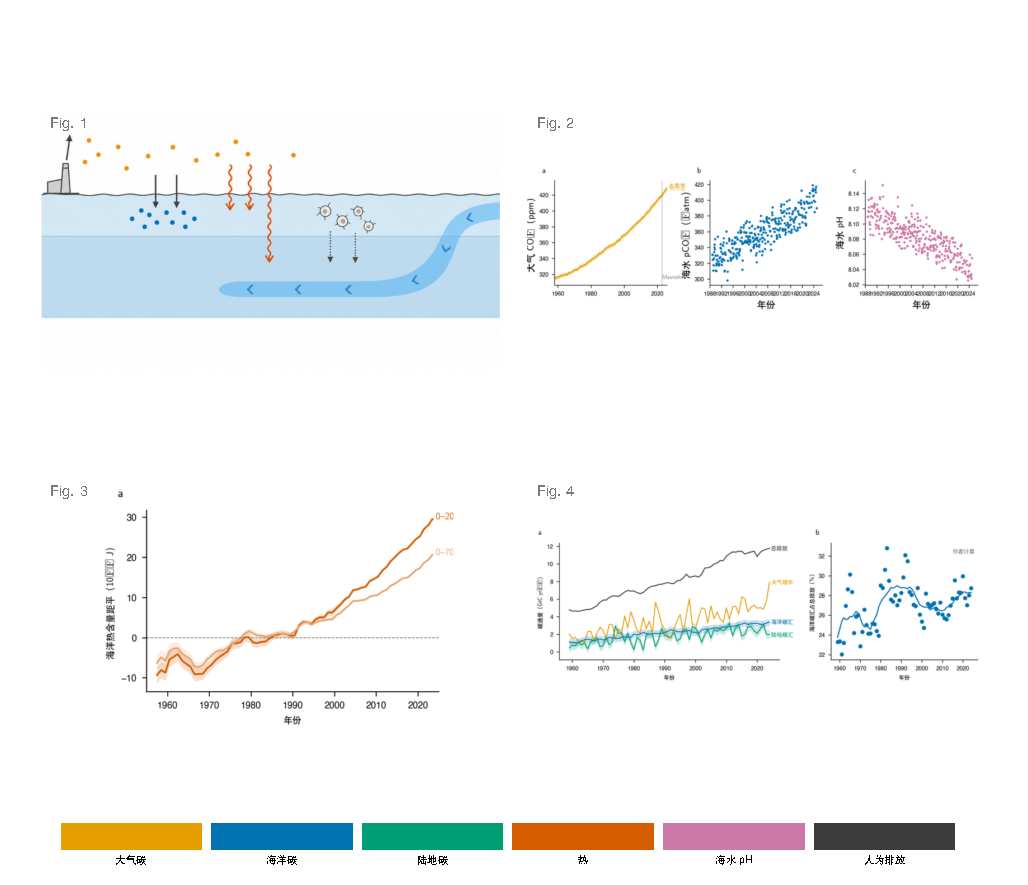
\includegraphics[width=\linewidth]{figures/ch04/ch04-08-consistent-set-zh.pdf}
\caption{按同一页视觉规范修改后的四张论文图。每种颜色在全文中只代表一类物理量或碳库（底部色条），字体、字号、面板编号、线型与箭头形状统一。与图~\ref{fig:ch04-01} 相比，底层数据完全相同，只改变了视觉语言。}\label{fig:ch04-08}
\end{figure}

对比图~\ref{fig:ch04-08} 与图~\ref{fig:ch04-01}，读者无需反复查阅图例框，就能顺着橙色（大气碳）串起 Fig.\ 1、Fig.\ 2a 与 Fig.\ 4a，顺着蓝色（海洋碳）串起 Fig.\ 1、Fig.\ 2b 与 Fig.\ 4a/b，顺着朱红色（热量）串起 Fig.\ 1 与 Fig.\ 3。除图~\ref{fig:ch04-05}–\ref{fig:ch04-07} 已给出的图注外，论文 Fig.\ 1 的完整图注定稿如下，四张图的跨图总核验记录见表~\ref{tab:ch04-verify}。

\begin{BookNote}
\textbf{论文图 1 图注定稿：} \textbf{图 1　海洋吸收热量与人为 $\text{CO}_2$ 的主要途径示意。} 大气中增加的热量经海气界面进入表层混合层（波浪箭头），并随混合与水体下沉输送到海洋内部（浅蓝带）。人为排放的 $\text{CO}_2$ 经海气交换溶入表层海水（直线箭头），使海水 $p\text{CO}_2$ 升高、pH 降低，并同样随水体输运进入内部。浮游植物固定碳并以下沉颗粒形式输出（点线箭头），这一生物泵主要转运自然碳循环中的碳；人为 $\text{CO}_2$ 的吸收主要由海气交换、海水化学与环流决定。示意图，不按比例；省略了区域差异、季节变化、海冰、沉积物与河流输入。依据 Sabine 等（2004）、Gruber 等（2019）与 IPCC AR6 第一工作组第 5、9 章整理。
\end{BookNote}

\begin{table}[htbp]\centering\footnotesize
\setlength{\tabcolsep}{3pt}
\renewcommand{\arraystretch}{1.15}
\caption{主案例四张论文图的跨图总核验记录。}\label{tab:ch04-verify}
\begin{tabularx}{\linewidth}{@{}>{\raggedright\arraybackslash}p{38mm}YYYY@{}}
\toprule
\textbf{核验项目} & \textbf{Fig.\ 1} & \textbf{Fig.\ 2} & \textbf{Fig.\ 3} & \textbf{Fig.\ 4} \\
\midrule
语义色符合规范 A（跨图同色同义） & 通过（色值近似） & 通过 & 通过 & 通过 \\
色觉模拟与灰度下同面板可分 & 靠形状冗余可分 & 分面板无冲突 & 通过（图~\ref{fig:ch04-03}） & 通过（加直接标注） \\
100\% 尺寸字号符合 8/7/6 pt & 通过 & 通过 & 通过 & 通过 \\
面板字母与单位一致，无缺字裁切 & 浮游植物标签待右移 & 下标 2 与末端重叠待修 & 右端标签被裁待扩边距 & 上标负号遗失待修 \\
线型与箭头符合表~\ref{tab:ch04-lines}、\ref{tab:ch04-arrows} & 通过 & 通过 & 通过 & 通过 \\
起止年份与行数同原文件一致 & — & 823 行 / 346 点 & 67 行（双深度一致） & 66 行（1959–2024） \\
作者计算项与不确定性已入图注 & — & pH 标度待核文档 & 基准期待核文档 & 已标“作者计算” \\
数据引用完整，领域同行复核 & 待海洋同行复核 & 已含 NOAA / Scripps / HOT & 已含 NCEI / Levitus & 已含 GCB 2025 \\
\bottomrule
\end{tabularx}
\end{table}

\section{AI 在这一步能做什么与不能做什么}

在建立并执行整篇论文视觉语言的过程中，AI 工具与作者的职责边界汇总于表~\ref{tab:ch04-01}。

\begin{table}[htbp]\centering\footnotesize
\setlength{\tabcolsep}{3pt}
\renewcommand{\arraystretch}{1.15}
\caption{在建立整篇论文视觉语言环节，AI 能做什么、不能做什么及作者要核对的内容。}\label{tab:ch04-01}
\begin{tabularx}{\linewidth}{@{}>{\raggedright\arraybackslash}p{18mm}YYY@{}}
\toprule
\textbf{环节} & \textbf{AI 能做} & \textbf{AI 不能做 / 不可靠} & \textbf{作者要核对} \\
\midrule
起草规范 & 对话式 AI 可根据图清单提出语义色分配、字号层级的初稿，并推荐色觉友好的色板 & 不知道你所在领域的颜色惯例和目标期刊要求；可能推荐不存在或已撤稿的“依据” & 规范条款逐条确认；引用用 Crossref 查 DOI 与撤稿状态 \\
跨图记忆 & — & \scidraw{} 目前没有项目级风格设置，不会在不同会话、不同工具之间记住你的规范 & 规范保存为文档；每次新会话粘贴风格块 \\
数据图套用样式 & \sdtool{sci-vis} 可按风格块生成图，并在对话中逐项修改；可恢复历史版本 & 多轮修改后可能悄悄改回默认颜色、字号或加回图例；“已按规范”的回答不等于做到了 & 每次修改后取色、量字号、对线型表；保存每个满意版本 \\
数据完整性 & \sdtool{sci-vis} 对上传的源数据做哈希、字节数与行数校验 & 校验只证明输入没丢，不证明单位、标度、基准期或计算正确 & 起止时间、行数、单位、基准期对照原始文件与数据说明 \\
示意图套用样式 & 绘图与参考图修改可按风格块生成扁平示意并调整颜色 & 色值、线宽只能近似；可能出现局部流向矛盾或加入未要求的对象 & 多次候选比选；逐色取色；对照箭头表；删去多余对象并校准标签位置 \\
色觉与技术检查 & \sdtool{figure-checker} 可做格式、分辨率、色彩、灰度与色觉风险等技术检查 & 不审核科学内容；色觉模拟是近似，不能代替询问色觉差异读者 & 用模拟 + 灰度 + 至少一位读者确认；科学内容另行核验 \\
图注 & \sdtool{figure-legend} 可根据图片起草图注 & 不知道数据来源、处理、基准期；不得让它补写这些信息 & 来源、单位、作者计算项、不确定性含义由作者填写 \\
\bottomrule
\end{tabularx}
\end{table}

\section{本章检查清单}

\begin{itemize}
\item 我有一页书面的视觉规范，并给它标了版本号。
\item 每个语义色只表示一类量，每类量只用一个语义色；跨所有图核对过。
\item 语义色不超过 6–7 个，其余元素用灰。
\item 同一面板中的颜色在色觉模拟和灰度下仍可区分，或另有形状、线型、直接标注作冗余。
\item 连续变量用感知均匀的顺序或发散色图，没有使用彩虹色图。
\item 字号在最终印刷尺寸下量过：面板字母、轴标签、刻度、注释四级一致。
\item 全文一种字体；中英文版位置与字号一致，且检查了上下标与特殊字符无缺字。
\item 单位写法、面板字母写法在所有图中相同。
\item 每种线型、每种箭头形状只有一个含义，图例中定义一次。
\item 图标用中性色，没有未讨论的装饰对象。
\item 风格块在每次新会话中重新粘贴，每次修改后都复查了颜色和字号。
\item 数据图的来源、下载日期、处理方式、作者计算项都写进了图注。
\item 我把所有图按最终尺寸放在一页上看过一次。
\end{itemize}

\section{练习}

\begin{enumerate}
\item \textbf{（纸笔：给你的论文分配语义色）} 列出你正在写的论文（或一篇你熟悉的论文）中所有图里出现的“量”或“类别”。（a）把它们合并成不超过 6 类；（b）为每类指定一个 Okabe–Ito 色并写出“用于 / 不用于”；（c）找出现有图中违反这张表的地方，至少三处，写出修改方案；（d）说明你的学科有没有必须遵守的颜色惯例（例如温度暖色、降水蓝绿），你的分配是否与之冲突。
\item \textbf{（色觉与灰度检查）} 选你论文中的一张数据图。（a）导出 PNG，用 \scidraw{} 图片检查（\sdtool{figure-checker}）查看色觉风险与灰度结果，或用 \texttt{colorspacious} 自行模拟三种色觉差异；（b）指出哪一对颜色在模拟下最难区分；（c）在不增加新色相的前提下，用明度、线型或直接标注解决这个问题；（d）说明为什么模拟结果不能代替询问真实读者。
\item \textbf{（\scidraw{} 实操：同一份数据，用风格块约束）} 从 NOAA GML 下载 \texttt{co2\_mm\_mlo.csv}，去掉以 \texttt{\#} 开头的注释行，另存为纯 CSV（记录 SHA-256 与行数）。（a）在 \scidraw{} 科学可视化（\sdtool{sci-vis}）中上传该文件，只说“画大气 $\text{CO}_2$ 时间序列”，保存结果；（b）新开会话，上传同一文件，粘贴本章的数据图风格块再提出同样要求；（c）再追加两轮修改（例如“把月均值改成更浅”“在 2022 年 12 月处加一条细竖线”），检查每轮后颜色与字号是否仍符合规范，记录任何漂移；（d）对比（a）（b）（c）三版，交一份逐项核对表（颜色、字号、线型、标注、数据行数），并写出致谢 NOAA GML 与 Scripps 的一句话。（注：本章示例图由图像模型与配套脚本生成，提示词与生成记录见本书仓库。）
\end{enumerate}

\section*{参考文献}

{\sloppy
\begin{itemize}
\item Brewer CA. ColorBrewer 2.0: Color advice for cartography. \url{https://colorbrewer2.org}
\item Canadell JG, Monteiro PMS, Costa MH, Cotrim da Cunha L, Cox PM, Eliseev AV, Henson S, Ishii M, Jaccard S, Koven C, Lohila A, Patra PK, Piao S, Rogelj J, Syampungani S, Zaehle S, Zickfeld K. Global carbon and other biogeochemical cycles and feedbacks. In: \textit{Climate Change 2021: The Physical Science Basis. Contribution of Working Group I to the Sixth Assessment Report of the Intergovernmental Panel on Climate Change}. Cambridge University Press; 2023:673--816. doi:10.1017/9781009157896.007
\item Crameri F, Shephard GE, Heron PJ. The misuse of colour in science communication. \textit{Nature Communications}. 2020;11:5444. doi:10.1038/s41467-020-19160-7
\item Dore JE, Lukas R, Sadler DW, Church MJ, Karl DM. Physical and biogeochemical modulation of ocean acidification in the central North Pacific. \textit{Proceedings of the National Academy of Sciences}. 2009;106(30):12235--12240. doi:10.1073/pnas.0906044106
\item Fox-Kemper B, Hewitt HT, Xiao C, Aðalgeirsdóttir G, Drijfhout SS, Edwards TL, Golledge NR, Hemer M, Kopp RE, Krinner G, Mix A, Notz D, Nowicki S, Nurhati IS, Ruiz L, Sallée J-B, Slangen ABA, Yu Y. Ocean, cryosphere and sea level change. In: \textit{Climate Change 2021: The Physical Science Basis. Contribution of Working Group I to the Sixth Assessment Report of the Intergovernmental Panel on Climate Change}. Cambridge University Press; 2023:1211--1362. doi:10.1017/9781009157896.011
\item Friedlingstein P, O'Sullivan M, Jones MW, et al. Global Carbon Budget 2025. \textit{Earth System Science Data}. 2026;18:3211--3288. doi:10.5194/essd-18-3211-2026
\item Gruber N, Clement D, Carter BR, Feely RA, van Heuven S, Hoppema M, Ishii M, Key RM, Kozyr A, Lauvset SK, Lo Monaco C, Mathis JT, Murata A, Olsen A, Perez FF, Sabine CL, Tanhua T, Wanninkhof R. The oceanic sink for anthropogenic $\text{CO}_2$ from 1994 to 2007. \textit{Science}. 2019;363(6432):1193--1199. doi:10.1126/science.aau5153
\item Krzywinski M. Elements of visual style. \textit{Nature Methods}. 2013;10(5):371. doi:10.1038/nmeth.2444
\item Levitus S, Antonov JI, Boyer TP, Baranova OK, Garcia HE, Locarnini RA, Mishonov AV, Reagan JR, Seidov D, Yarosh ES, Zweng MM. World ocean heat content and thermosteric sea level change (0--2000 m), 1955--2010. \textit{Geophysical Research Letters}. 2012;39:L10603. doi:10.1029/2012GL051106
\item NOAA Global Monitoring Laboratory. Trends in Atmospheric Carbon Dioxide (Mauna Loa, Hawaii) and Scripps Institution of Oceanography $\text{CO}_2$ Program. \url{https://gml.noaa.gov/ccgg/trends/} and \url{https://scrippsco2.ucsd.edu/}
\item Nuñez JR, Anderton CR, Renslow RS. Optimizing colormaps with consideration for color vision deficiency to enable accurate interpretation of scientific data. \textit{PLOS ONE}. 2018;13(8):e0199239. doi:10.1371/journal.pone.0199239
\item Okabe M, Ito K. Color Universal Design (CUD): How to make figures and presentations that are friendly to colorblind people. 2008. \url{https://jfly.uni-koeln.de/color/}
\item Rougier NP, Droettboom M, Bourne PE. Ten simple rules for better figures. \textit{PLoS Computational Biology}. 2014;10(9):e1003833. doi:10.1371/journal.pcbi.1003833
\item Sabine CL, Feely RA, Gruber N, Key RM, Lee K, Bullister JL, Wanninkhof R, Wong CS, Wallace DWR, Tilbrook B, Millero FJ, Peng T-H, Kozyr A, Ono T, Rios AF. The oceanic sink for anthropogenic $\text{CO}_2$. \textit{Science}. 2004;305(5682):367--371. doi:10.1126/science.1097403
\item von Schuckmann K, Minière A, Gues F, Cuesta-Valero FJ, Kirchengast G, Adusumilli S, Straneo F, et al. Heat stored in the Earth system 1960--2020: where does the energy go? \textit{Earth System Science Data}. 2023;15(4):1675--1709. doi:10.5194/essd-15-1675-2023
\item Wong B. Points of view: Color coding. \textit{Nature Methods}. 2010;7(8):573. doi:10.1038/nmeth0810-573
\item Wong B. Points of view: Typography. \textit{Nature Methods}. 2011;8(4):277. doi:10.1038/nmeth0411-277
\item Wong B. Points of view: Color blindness. \textit{Nature Methods}. 2011;8(6):441. doi:10.1038/nmeth.1618 (Author Correction: \textit{Nature Methods}. 2023;20:1442. doi:10.1038/s41592-023-01974-0)
\end{itemize}
\par}

\chapter{用 AI 辅助数据可视化}

生态学专业的研究生林悦刚整理完一份南极帕默群岛（Palmer Archipelago）三种企鹅繁殖成体的形态测量数据表。为了在组会汇报和论文“研究对象”一节展示三种企鹅的体重差异，她打开一个支持对话的数据可视化工具，上传表格后输入了一句：“帮我画一张专业的企鹅体重比较图，要符合期刊风格。”几秒钟后，屏幕上出现了一张配色明快、排版端正的柱状图：三根彩色柱子代表三种企鹅，每根柱子顶端各立着一小段黑色误差线。

初看之下，这张图干净利落，似乎可以直接放进手稿。然而在组会上，导师接连问出四个最基本的问题，林悦却一个也答不上来：第一，柱顶那截短短的误差线究竟表示标准差（SD）、标准误（SEM）还是 95\% 置信区间？第二，每根柱子背后分别汇总了多少条测量记录，表里的缺失值被工具怎么处理了？第三，企鹅体重存在明显的雌雄二态性，把雌雄混在一根柱子里算均值，掩盖了多少物种内部的性别差异？第四，为什么前两种企鹅的平均体重只相差三十多克，在另一张自动缩放纵轴的草图里却看起来差了将近一倍？

数据图在论文中不是点缀版面的装饰画，而是直接支撑科学结论的定量证据。对话式可视化工具可以帮我们省去查阅绘图函数语法的繁琐时间，但只要输入的指令含糊不清，工具就会在后台替作者做出一连串未经授权的统计汇总与视觉编码决定。因此，面对任何一张 AI 生成或辅助修改的数据图，我们要问的第一个问题从来不是“这张图好不好看”，而是“这张图对不对、诚不诚实、能不能经得起逐项核对”。本章从读懂一张原始数据表开始，系统拆解如何用 AI 工具辅助制作、修改并严格核验科研数据图。

\section{先读表，再选图}

拿到数据表后直接拖进绘图工具并让 AI“推荐最合适的图”，是造成后续反复返工甚至发表错误图表的常见根源。软件只能读取列名和数值格式，却看不到数据背后的采样过程与实验设计。在动手画图之前，作者必须先替 AI 完成四项“读表”工作。

\textbf{第一，确认每一行代表什么观测单位。}这是最容易被 AI 误判、也最容易被作者略过的一步。本章主案例使用南极帕默站长期生态研究项目（Palmer Station LTER）采集、由 Horst 等（2020）整理发布的公开企鹅数据集（\texttt{palmerpenguins} v0.1.0，CC0 许可；原始生态学研究见 Gorman 等，2014）。清理后的数据表 \texttt{penguins.csv} 共 344 行、8 列。如果你把这张表传给 AI 并直接提问“表里有多少只企鹅”，AI 会毫不犹豫地回答“344 只”。但只要查阅原始数据包说明就会发现，原始记录中的个体编号（\texttt{Individual ID}，如 \texttt{N21A1}）采用的是按筑巢位置编码的规则，在 344 行记录中有 60 个“物种 + 个体编号”组合在 2007—2009 三个研究季之间重复出现。单凭清理后的表格，未经逐一核实原始野外记录，并不能直接断言“每一行都是一只不同的企鹅个体”。因此，最严谨、保守的表述是把每一行定义为\textbf{一条繁殖成体的形态测量记录}，并在任务书和图注中明确写为“$n = \text{记录数}$”。AI 可以快速统计表格行数，却看不出编码规则背后的生态学采样逻辑，这种界定必须由作者亲自完成。

\textbf{第二，清点变量类型、物理单位与记录精度。}打开表格后，应逐列区分哪些是分类分组变量，哪些是连续测量变量，哪些是时间或批次标记，并整理成数据字典（表~\ref{tab:ch05-dict}）。这里需重点防范两类陷阱：一是\textbf{用整数编码的批次标记}，如表中的 \texttt{year} 列取值为 2007、2008、2009，在软件眼里它是标准数值列，若不加说明，自动绘图功能常会把它当成连续测量变量去算“平均年份”或画进相关性矩阵，而实际上它只是三个采样研究季的批次标记；二是\textbf{原始测量的最小刻度}，如鳍肢长度记录到整数毫米，体重（\texttt{body\_mass\_g}）在野外称重时以 $25\ \text{g}$ 或 $50\ \text{g}$ 为最小刻度记录整数，后续若在图上标出三位小数就会制造伪精度。

\begin{table}[htbp]\centering\footnotesize
\setlength{\tabcolsep}{3pt}
\renewcommand{\arraystretch}{1.15}
\caption{帕默企鹅数据集（\texttt{penguins.csv}，共 344 行）的数据字典。}\label{tab:ch05-dict}
\begin{tabularx}{\linewidth}{@{}l>{\raggedright\arraybackslash}p{26mm}cY c@{}}
\toprule
\textbf{列名} & \textbf{类型} & \textbf{单位} & \textbf{说明} & \textbf{缺失} \\
\midrule
\texttt{species} & 分类（3 水平） & — & 阿德利（Adelie）/ 帽带（Chinstrap）/ 巴布亚（Gentoo） & 0 \\
\texttt{island} & 分类（3 水平） & — & Biscoe / Dream / Torgersen；巴布亚仅见于 Biscoe，帽带仅见于 Dream，阿德利三岛均有 & 0 \\
\texttt{bill\_length\_mm} & 连续 & mm & 嘴峰长度（沿嘴峰上缘测量的喙长） & 2 \\
\texttt{bill\_depth\_mm} & 连续 & mm & 嘴峰深度（闭合喙部的竖直高度） & 2 \\
\texttt{flipper\_length\_mm} & 连续（整数） & mm & 鳍肢长度 & 2 \\
\texttt{body\_mass\_g} & 连续（整数） & g & 体重（野外记录到 $25\ \text{g}$ 或 $50\ \text{g}$ 量级） & 2 \\
\texttt{sex} & 分类（2 水平） & — & \texttt{female}（雌）/ \texttt{male}（雄） & 11 \\
\texttt{year} & 整数 & — & 2007 / 2008 / 2009，研究季标记，不是测量值 & 0 \\
\bottomrule
\end{tabularx}
\end{table}

\textbf{第三，核查缺失值（NA）的数量与重叠关系。}表~\ref{tab:ch05-dict} 中四个形态测量列各缺 2 行（记作字符串 \texttt{NA}），而性别列有 11 行缺失；进一步核对可知，体重缺失的那 2 行同时也缺失性别。这一事实直接决定了不同分析视角下的有效样本量：如果只按物种汇总体重或嘴峰尺寸，剔除测量值缺失的 2 行后有效记录数为 $n = 342$；如果按“物种 $\times$ 性别”交叉分组分析体重，则需剔除性别或体重为 \texttt{NA} 的共 11 行，保留有效记录数 \textbf{$n = 333$}。若不在指令中写明剔除规则，绘图工具要么静默删行而不报告样本量，要么把字符串 \texttt{"NA"} 当成第三个性别组画在横轴上。

\textbf{第四，识别分类混杂与研究设计。}注意表~\ref{tab:ch05-dict} 中 \texttt{island} 列的分布：Torgersen 岛全部是阿德利企鹅（52 条），Biscoe 岛只有阿德利（44 条）和体型庞大的巴布亚企鹅（124 条），Dream 岛则只有阿德利（56 条）和帽带企鹅（68 条）。若不看数据字典就直接画“三个岛的企鹅平均体型对比”，Biscoe 岛会显得格外重——但这并非岛屿环境造就的同种差异，而是因为巴布亚企鹅只在该岛采样。同样，不同行之间究竟是独立组、配对前后测、重复测量还是时间序列，直接决定了候选图型家族与图上必须保留的信息（表~\ref{tab:ch05-01}）。

\begin{table}[htbp]\centering\footnotesize
\setlength{\tabcolsep}{3pt}
\renewcommand{\arraystretch}{1.15}
\caption{研究设计与数据结构对应的候选图型及常见 AI 默认错误。}\label{tab:ch05-01}
\begin{tabularx}{\linewidth}{@{}>{\raggedright\arraybackslash}p{28mm}>{\raggedright\arraybackslash}p{25mm}YY@{}}
\toprule
\textbf{研究设计 / 数据结构} & \textbf{候选图型} & \textbf{必须保留的信息} & \textbf{常见 AI 默认错误} \\
\midrule
少数独立组的连续测量（每组 $n < \text{约 }30$） & 散点 + 均值/中位数、箱线 + 散点 & 所有观测点、每组 $n$ & 只画均值柱 + SEM \\
独立组、$n$ 较大 & 箱线图、小提琴图、云雨图 & 分布形状、$n$、离群值 & 小提琴图把 $n$ 隐藏；核密度平滑过度 \\
配对 / 前后测 & 配对点线图、差值图 & 配对键、个体轨迹、方向不同的对象 & 当作两独立组；删“异常”对象 \\
重复测量多个时间点 & 个体轨迹 + 均值线；分面 & 个体 ID、时间间隔真实比例 & 时间当分类变量、等距排布不等距时间 \\
时间序列 & 折线（连续时间轴） & 缺测/插补标记、测量方法变化 & 双纵轴；平滑掉季节信号不说明 \\
两个连续变量 & 散点（+分组颜色/形状）、必要时拟合线 & 分组结构、$n$、拟合方法 & 全体一条回归线；图上堆 $p$ 值 \\
矩阵 / 二维场 & 热图（感知均匀色图） & 色标、单位、数值范围 & 彩虹色图；色标不标单位 \\
\bottomrule
\end{tabularx}
\end{table}

\section{分组比较：同一份数据，四种画法}

比较几个独立分组的连续测量值时，最核心的权衡在于：\textbf{把原始观测汇总到什么程度？}汇总得越激进，画面越简单，被隐藏的数据结构也越多。我们取剔除 2 条体重缺失记录后的 $n = 342$ 条企鹅记录（阿德利 151、帽带 68、巴布亚 123），用四种常见图型展示同一份数据（图~\ref{fig:ch05-01}）。全章企鹅图统一采用对色觉异常友好的 Okabe–Ito 配色：阿德利橙色（\texttt{\#E69F00}）、帽带天蓝（\texttt{\#56B4E9}）、巴布亚蓝绿（\texttt{\#009E73}）。

\begin{figure}[htbp]\centering
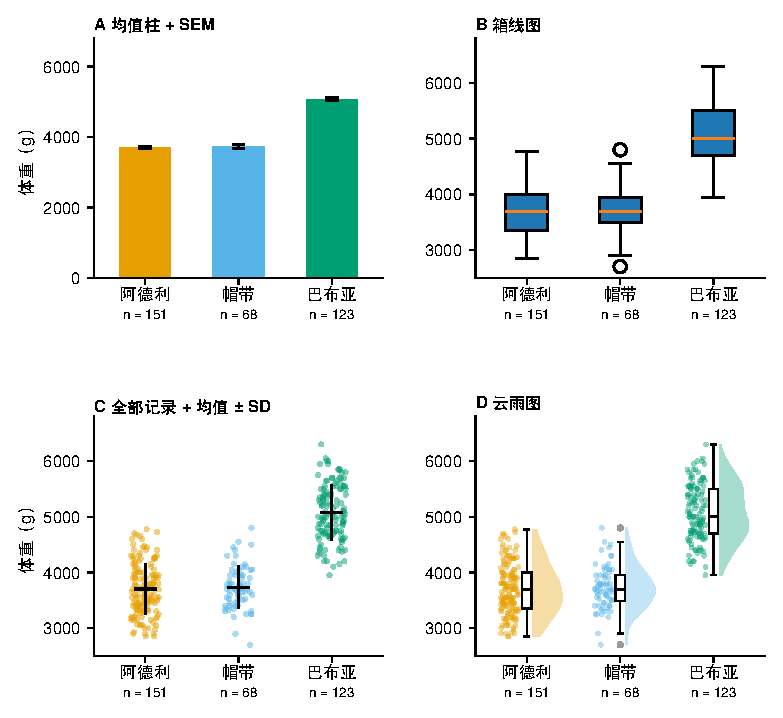
\includegraphics[width=\linewidth]{figures/ch05/ch05-01-group-forms-zh.pdf}
\caption{同一组数据的四种表达。三种企鹅体重（palmerpenguins，$n = 342$ 条记录；剔除体重缺失 2 条）。A 均值柱与 $\pm 1\ \text{SEM}$；B 箱线图（须为 $1.5$ 倍四分位距）；C 全部记录与均值 $\pm 1\ \text{SD}$；D 云雨图（核密度、箱线与原始点）。A 只呈现 6 个数，看不出帽带企鹅的记录数不到阿德利的一半，也看不到分布形状。}\label{fig:ch05-01}
\end{figure}

对照图~\ref{fig:ch05-01} 的四个面板，可以清楚看到每种画法的得失：

\begin{itemize}
\item \textbf{面板 A（均值柱 + SEM）：把 342 条记录压缩成 6 个数。}面板 A 的纵轴诚实地从 $0\ \text{g}$ 起步，但它只给出了 3 个均值（$3700.7\ \text{g}$、$3733.1\ \text{g}$、$5076.0\ \text{g}$）和 3 个均值标准误（$37.3\ \text{g}$、$46.6\ \text{g}$、$45.5\ \text{g}$）。柱顶的 SEM 误差线在数千克尺度上短得几乎缩成一条黑线。若不在横轴下方专门标出 $n$，三根等宽的柱子完全掩盖了帽带企鹅记录数（$n=68$）还不到阿德利（$n=151$）一半的事实；同时，$0\text{--}2700\ \text{g}$ 之间没有任何成体企鹅记录，实心柱却占去近半画幅，真正有数据分布的区间反而被挤压。Weissgerber 等（2015）指出，完全相同的柱子加误差线可能对应正态、偏态、双峰或含极端值的分布，中小样本比较应优先展示原始观测点。

\item \textbf{面板 B（箱线图）：展示分位数与离群点，但仍隐藏 $n$ 与亚群。}面板 B 将纵轴聚焦在 $2500\text{--}6800\ \text{g}$（箱线图不靠柱体面积编码数值，纵轴可不从 0 开始）。箱内橙线为中位数（阿德利与帽带均为 $3700\ \text{g}$，巴布亚为 $5000\ \text{g}$），箱体上下缘为第一、三四分位数（四分位距 IQR），须线延伸至 $1.5 \times \text{IQR}$。此时面板 A 隐藏的一个特征显露出来：帽带企鹅上下两端各有一个超出 $1.5 \times \text{IQR}$ 的空心圆离群点（最低值 $2700\ \text{g}$ 与最高值 $4800\ \text{g}$）。但箱体宽度本身仍不反映样本量差异，且当组内包含雌雄两个亚群时，单一箱体依然会把潜在的双峰结构合并成一个长方形。

\item \textbf{面板 C（全部记录 + 均值 $\pm$ SD）：把每一个观测点还给读者。}面板 C 将 342 条记录全部画成半透明散点，并叠加黑色短横线（均值）与竖线（$\pm 1\ \text{SD}$）。读者一眼就能读出三层信息：第一，中间天蓝色的帽带企鹅点云明显比两侧稀疏；第二，各物种内部个体体重跨度达近两千克（阿德利 $2850\text{--}4775\ \text{g}$，帽带 $2700\text{--}4800\ \text{g}$，巴布亚 $3950\text{--}6300\ \text{g}$），均值 $\pm 1\ \text{SD}$ 竖线如实反映了点云的主体离散宽度；第三，两端极值点自然呈现在点云上下边界，无需依赖人为须线阈值即可看清。

\item \textbf{面板 D（云雨图，Raincloud plot）：分布轮廓、箱线与原始点三合一。}按 Allen 等（2019）的设计，面板 D 在每组左侧画横向抖动的原始点（“雨”），中间放窄白底箱线图，右侧画截断在各组极值范围内的半边核密度估计曲线（“云”）。右侧平滑的密度轮廓能直观揭示点云内部的聚集形态——例如巴布亚企鹅（右侧蓝绿）的密度曲线在 $4700\ \text{g}$ 与 $5500\ \text{g}$ 附近呈现出宽肩形态，恰好提示该物种内部包含雌雄两个亚群。
\end{itemize}

据此可以定下一条清晰的选图原则：\textbf{当每组样本量较小或中等（几条至百余条）时，优先展示全部原始点（面板 C 或 D）；当每组样本量极大、散点完全重叠成墨团时，使用箱线图、小提琴图或云雨图，并务必在横轴下方标明每组的 $n$。}在 \scidraw{} 科学可视化（\sdtool{sci-vis}）中要求展示原始散点时，必须在对话指令中明确说明\textbf{随机抖动只改变横坐标，不改变纵坐标数值}：

\begin{Prompt}
改为分组散点图：横轴为物种（阿德利、帽带、巴布亚），纵轴为体重（g），范围 2500–6800。
显示全部 342 条记录的原始点，点只在横向轻微随机抖动（不超过组间距的 15%）以减少重叠，
纵向测量数值绝不改变。每组叠加均值（短横线）与 ± 1 SD（竖线），横轴下方标出每组 n。
\end{Prompt}

\section{误差线到底表示什么}

对比图~\ref{fig:ch05-01} 面板 A 与面板 C：同样是阿德利企鹅的 151 条体重记录，为什么面板 A 柱顶的误差线只有短短几十克，而面板 C 点云中的误差线却长得多？因为面板 A 画的是均值标准误（SEM），面板 C 画的是样本标准差（SD）。把不同误差线混为一谈，或干脆不说明误差线类型，是科研论文配图的高发错误（Cumming 等，2007；Krzywinski 与 Altman，2013）。

三种常见误差线回答的是三个截然不同的问题（表~\ref{tab:ch05-err}）：

\begin{table}[htbp]\centering\footnotesize
\setlength{\tabcolsep}{2.5pt}
\renewcommand{\arraystretch}{1.15}
\caption{三种常见误差线的含义及在企鹅体重数据（$n=342$：阿德利 151、帽带 68、巴布亚 123）中的实际半宽对比。}\label{tab:ch05-err}
\begin{tabularx}{\linewidth}{@{}>{\raggedright\arraybackslash}p{18mm}>{\raggedright\arraybackslash}p{22mm}Yccc@{}}
\toprule
\textbf{误差线类型} & \textbf{计算公式} & \textbf{回答的科学问题与随 $n$ 变化的规律} & \textbf{阿德利} & \textbf{帽带} & \textbf{巴布亚} \\
\midrule
样本标准差（SD） & $s = \sqrt{\frac{\sum (x_i - \bar{x})^2}{n-1}}$ & \textbf{描述离散度：}个体测量值本身相差多大？随 $n$ 增大趋于稳定，不会因多测样本而变短 & $458.6\ \text{g}$ & $384.3\ \text{g}$ & $504.1\ \text{g}$ \\
均值标准误（SEM） & $\text{SEM} = s / \sqrt{n}$ & \textbf{估计精度：}样本均值离总体均值多远？随 $\sqrt{n}$ 增大而迅速缩短，不反映个体离散度 & $37.3\ \text{g}$ & $46.6\ \text{g}$ & $45.5\ \text{g}$ \\
95\% 置信区间半宽 & $t_{0.975,\,n-1} \times \text{SEM}$ & \textbf{区间估计：}总体均值的 95\% 估计区间半宽（大样本下约为 SEM 的 2 倍） & $73.7\ \text{g}$ & $93.0\ \text{g}$ & $90.0\ \text{g}$ \\
\bottomrule
\end{tabularx}
\end{table}

从表~\ref{tab:ch05-err} 的实测数据应牢记三条准则：
第一，\textbf{同一组数据的 SD 与 SEM 可相差十倍以上}。阿德利企鹅的 $\text{SD} = 458.6\ \text{g}$，除以 $\sqrt{151} \approx 12.29$ 后得到的 $\text{SEM}$ 仅为 $37.3\ \text{g}$，$95\%\ \text{CI}$ 半宽约为 $73.7\ \text{g}$。若想向读者展示个体体重本身的波动范围，必须用 SD（或四分位距）；若想展示总体均值的估计区间，优先用 95\% CI，切勿为了追求“误差线短、显得数据漂亮”而选用 SEM。
第二，\textbf{所有误差线都必须在图例或图注中写明统计类型与每组 $n$}，只有同时给出类型和 $n$，读者才能准确解读并在需要时换算。
第三，\textbf{不能凭误差线“重不重叠”直接断定差异是否显著}（Cumming 等，2007；Krzywinski 与 Altman，2013）。当图上画的是 $\pm 1\ \text{SD}$ 时，两条误差线大幅重叠，两组均值仍可能高度显著不同；当画的是独立样本的 $\pm 1\ \text{SEM}$ 时，即便两条误差线刚刚不重叠，双侧 $p$ 值仍大于 $0.05$（两独立且样本量相近的大样本，SEM 误差线需留出约 0.5–1 倍 SEM 的空隙，或两条 95\% CI 重叠不超过单侧臂长的约四分之一，才大致对应 $p \le 0.05$）。

由于许多 AI 绘图工具默认绘制最短的 SEM 且不加说明，作者在 \sdtool{sci-vis} 中必须明确点名误差线统计量：

\begin{Prompt}
误差线请统一使用样本标准差（± 1 SD，ddof = 1），不要使用标准误（SEM）。
在图例中写明“横线：均值；竖线：± 1 SD”，在横轴每组下方标注样本量 n，不画星号或 p 值。
\end{Prompt}

\section{配对与重复测量}

当两列数值来自同一批研究对象在处理前后的两次测定（或同一样点在两个时期的复测），数据就具有一一对应的\textbf{配对结构（paired structure）}。我们延续第 1、2 章使用的模拟教学数据集（\texttt{paired-example.csv}，CC BY 4.0）：8 个虚构对象（\texttt{SIM01}–\texttt{SIM08}），前测均值 $13.125\ \text{a.u.}$，后测均值 $16.5\ \text{a.u.}$，各对象差值（后测 $-$ 前测）依次为 $+4, +3, +4, -1, +4, +5, +4, +4$，均值差 $3.375\ \text{a.u.}$。图~\ref{fig:ch05-03} 对比了这份配对数据的三种画法。

\begin{figure}[htbp]\centering
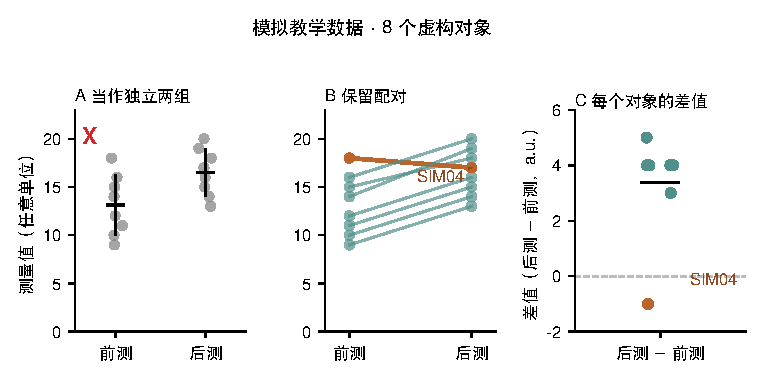
\includegraphics[width=\linewidth]{figures/ch05/ch05-03-paired-views-zh.pdf}
\caption{配对数据的三种画法（模拟教学数据）。8 个虚构对象各测量两次。A 把两列当作独立组，配对信息消失，读者可能以为有 16 个对象；B 保留每个对象的前后连线，\texttt{SIM04} 下降可见；C 直接展示每个对象的差值，7 个为正、1 个为负，均值差 $3.375\ \text{a.u.}$。未进行显著性检验。}\label{fig:ch05-03}
\end{figure}

观察图~\ref{fig:ch05-03} 三个面板的实际画面：
\begin{itemize}
\item \textbf{面板 A（当作独立两组，左上角标红色“X”）：丢失配对的错误画法。}面板 A 只把前测和后测画成两列孤立的灰色散点与均值 $\pm\ \text{SD}$。这会造成两个严重后果：一是画面上出现 16 个孤立散点，读者很容易误以为实验测量了 16 个独立对象；二是个体初始基线跨度很大（前测从 $9$ 到 $18$），组间基线差异完全淹没了组内变化，两列点的纵向区间大幅重叠，根本看不出每个对象在后测中究竟是升是降。
\item \textbf{面板 B（保留配对的斜率图 / 配对点线图）：呈现个体轨迹与逆向个体。}面板 B 用线段把同一对象的前测值与后测值连接起来。画面传达的信息瞬间清晰：8 个对象中有 7 条青绿色连线平行向右上倾斜（增幅 $+3$ 至 $+5$），唯独用暖棕色加粗标出的 \texttt{SIM04} 从前测最高基线 $18$ 降至后测的 $17$（变化量 $-1$）。当读者既关心对象的初始基线水平（例如 \texttt{SIM04} 基线最高，提示可能存在天花板效应），又关心变化方向是否一致时，应选用面板 B。
\item \textbf{面板 C（每个对象的差值图）：直接回答“变化了多少”。}当研究问题直接聚焦于“处理带来了多大的变化量”时，面板 C 以个体差值（后测 $-$ 前测）为纵轴画出 8 个差值点，用黑色短横线标出均值差 $3.375\ \text{a.u.}$，并在 $y = 0$ 处画一条灰色虚线作为“无变化”参考基线。7 个青绿色点落在零线上方 $+3$ 至 $+5$ 处（$+4$ 处的 5 个点横向微幅错开），棕色点 \texttt{SIM04} 落在零线下方 $-1$ 处。这里有一条硬性规范：\textbf{差值图的纵轴（本图为 $-2$ 至 $6$）必须包含 $0$ 并画出零参考线}，因为零线是判断增减方向的分界线。
\end{itemize}

使用 AI 工具绘制配对数据时，作者必须重点防范两项风险：一是工具忽略对象编号列（\texttt{sample\_id}），默认把前后两列当成两个独立组画成面板 A；二是当指令中出现“清理数据并突出主要趋势”等模糊表述时，部分自动脚本会把唯一逆向下降的 \texttt{SIM04} 当作“异常值”静默删掉。因此任务书中必须明确规定：“按 \texttt{sample\_id} 连线保留配对关系，完整保留全部 8 个对象，严禁剔除任何逆向变化或极端个体。”

\section{时间序列与双纵轴}

时间序列数据具有严格的先后顺序与时间比例，作图底线有两条：\textbf{横轴必须按真实时间间隔连续映射，数据说明中的插补与观测变更必须在图上留痕。}

本节使用地球与环境科学领域的经典观测记录——夏威夷莫纳罗亚（Mauna Loa）观测站大气 $\text{CO}_2$ 干空气摩尔分数月均值序列（Keeling，1960；由美国国家海洋和大气管理局全球监测实验室 NOAA GML 的 Xin Lan 博士与斯克里普斯海洋研究所 Scripps 的 Ralph Keeling 博士共同维护，公有领域，采用 WMO X2019 标度）。本案例锁定的公开数据快照（文件头创建日期为 2026 年 10 月 9 日）包含自 1958 年 3 月（$315.71\ \text{ppm}$）至 2026 年 9 月（$426.07\ \text{ppm}$）共 823 行月度记录，全时段最低月均值为 $312.42\ \text{ppm}$，最高月均值为 $432.34\ \text{ppm}$（2026 年 5 月）。图~\ref{fig:ch05-04} 展示了该序列的标准画法。

\begin{figure}[htbp]\centering
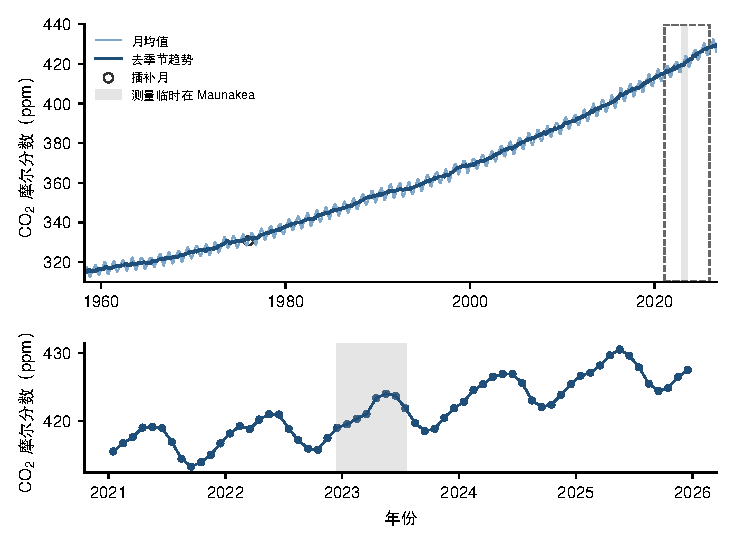
\includegraphics[width=\linewidth]{figures/ch05/ch05-04-co2-series-zh.pdf}
\caption{Mauna Loa 大气 $\text{CO}_2$ 月均值（1958 年 3 月至 2026 年 9 月快照）。上图（全时段）：细线为月均值，粗线为 NOAA 提供的去季节趋势值；空心圆为数据说明中的插补月（1975 年 12 月）；灰带为火山喷发后测量临时移至 Maunakea 的时段（2022 年 12 月至 2023 年 7 月）；右侧虚线框标出下图的放大范围。下图为最近 5 个完整年（2021—2025 年）的局部放大，可见明显的季节振荡。数据：NOAA GML（X.\ Lan）与 Scripps（R.\ Keeling），文件创建日期 2026 年 10 月 9 日；1974 年 5 月前为 Scripps 数据。}\label{fig:ch05-04}
\end{figure}

核对图~\ref{fig:ch05-04} 的上下两个面板，可以总结出时间序列作图的四项规范：
\begin{enumerate}
\item \textbf{连续数值时间轴：}横轴直接使用表中的十进制年份（\texttt{decimal date}），保证每一年、每个月的水平间距严格等比例，绝不把日期当成无序分类标签排列。
\item \textbf{原始观测与趋势分层并列：}上图同时绘出浅蓝细线（每月实测均值 \texttt{average}）与深蓝粗线（NOAA 官方去季节趋势 \texttt{deseasonalized}），不私自用未经说明的平滑滤波替掉原始波动。
\item \textbf{局部放大展示高频周期：}全时段近 70 年尺度下季节波动被压缩成密集细齿，因此上图右侧用虚线矩形框标出最近 5 个完整年（2021—2025 年），并在下图按 $2:1$ 高度比放大展示每月一个实心点的折线，清晰呈现北半球陆地植被生长季驱动的季节振荡（每年 5 月前后达峰、9—10 月见谷）。
\item \textbf{标出数据文件头注释中的特殊时段：}许多研究者读入 CSV 时直接跳过开头的 \texttt{\#} 注释行，却漏掉了关键背景。Mauna Loa 文件头注释明确记载：第一，1974 年 5 月前数据来自 Scripps，而自 1974 年 5 月 NOAA 独立观测以来，仅 1975 年 12 月因仪器故障无有效观测天数（\texttt{ndays} 为 $-1$），其数值为插补值——上图在 1975 年 12 月处专门用空心圆标出“插补月”；第二，2022 年 11 月底莫纳罗亚火山喷发切断站点供电与道路，2022 年 12 月至 2023 年 7 月测量临时移至约 21 英里外的莫纳克亚（Maunakea）山顶进行——上下两图均用浅灰色半透明竖带标出该时段。这些注释信息 AI 无法仅凭数字列猜出，必须由作者研读说明后要求标注。
\end{enumerate}

当需要同时展示两个量纲或量级不同的时间序列时，最常见的误导是\textbf{双纵轴（dual y-axes）}。我们取 Mauna Loa 完整日历年（1959—2025 年，共 67 年）的 12 个月均值算出年均浓度，再由相邻两年年均值之差算出 1960—2025 年（共 66 个值）的“年增长量”（单位：$\text{ppm/年}$；实测最小 $0.42$、最大 2024 年 $3.52\ \text{ppm/年}$，1960 年 $0.93$、2025 年 $2.74\ \text{ppm/年}$；注意这是相邻年均值之差，与 NOAA 官方按年末去季节值计算的年增长率算法不同，图注必须说明）。图~\ref{fig:ch05-06} 对比了双纵轴反例与上下分面正例。

\begin{figure}[htbp]\centering
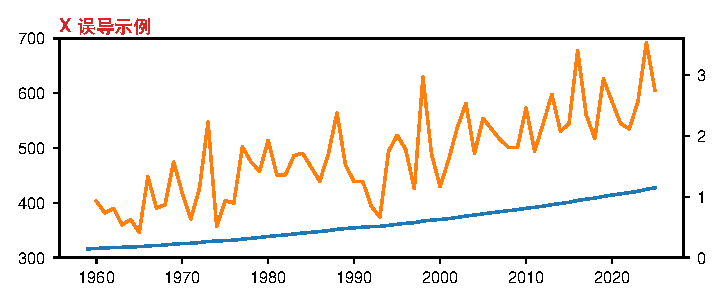
\includegraphics[width=\linewidth]{figures/ch05/ch05-06-dual-axis-bad-zh.pdf}\\[4pt]
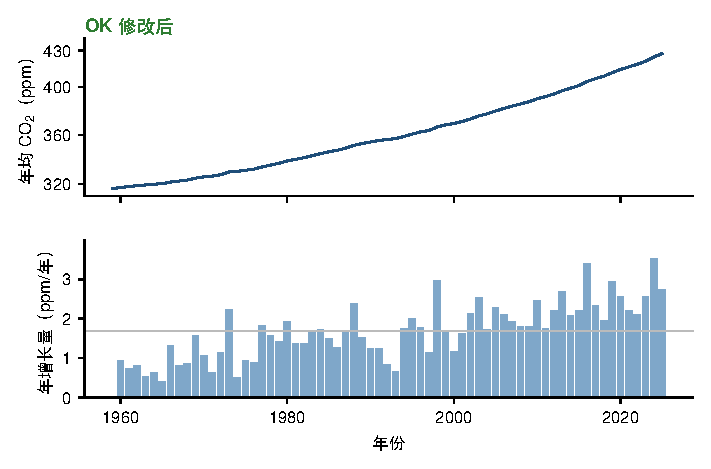
\includegraphics[width=\linewidth]{figures/ch05/ch05-06-dual-axis-good-zh.pdf}
\caption{双纵轴与分面（上为教学用错误示范）。上：年均 $\text{CO}_2$ 与年增长量共用一张图、两条纵轴，范围被人为选择，两线的相对位置没有意义。下：两个量各占一个面板，共享时间轴，增长量纵轴从 0 开始。年均值由 NOAA 月均值计算（仅完整年，1959—2025）；年增长量为相邻两年年均值之差，算法与 NOAA 官方增长率不同。}\label{fig:ch05-06}
\end{figure}

在图~\ref{fig:ch05-06} 上图（\texttt{X 误导示例}）中，左轴将年均浓度（蓝线）的范围人为拉大到 $300\text{--}700\ \text{ppm}$，把原本陡峭上升的浓度曲线压扁在底部；右轴将年增长量（橙线）设为 $0\text{--}3.6$ 撑满画幅，且左右两轴均无标题与单位。双纵轴的致命缺陷在于：\textbf{两条纵轴的起点与缩放比例可被任意调节}，作图者只需改动任一轴的范围，就能让两条线在任意年份“交叉”或“平行”，诱导读者从毫无物理意义的视觉交点中读出虚假关系。下图（\texttt{OK 修改后}）改用共享年份横轴的上下两个独立面板：上面板画年均浓度折线（$310\text{--}440\ \text{ppm}$），下面板用从 $0$ 开始的柱状图画年增长量（$0\text{--}4.0\ \text{ppm/年}$）并标出 1960—2025 年平均增长量参考线（浅灰横线，约 $1.69\ \text{ppm/年}$），既诚实保留各自量纲与基线，又方便顺着同一时间轴上下比对。

\section{散点与相关：分组变量会改变结论}

考察两个连续测量变量的关系时，若不向工具交代分类分组结构，AI 默认画出的“全体样本一条回归线”甚至会给出方向完全相反的结论。图~\ref{fig:ch05-08} 以企鹅嘴峰长度（\texttt{bill\_length\_mm}）与嘴峰深度（\texttt{bill\_depth\_mm}，剔除缺失 2 行后 $n = 342$）展示了教科书级的\textbf{辛普森悖论（Simpson's paradox）}。

\begin{figure}[htbp]\centering
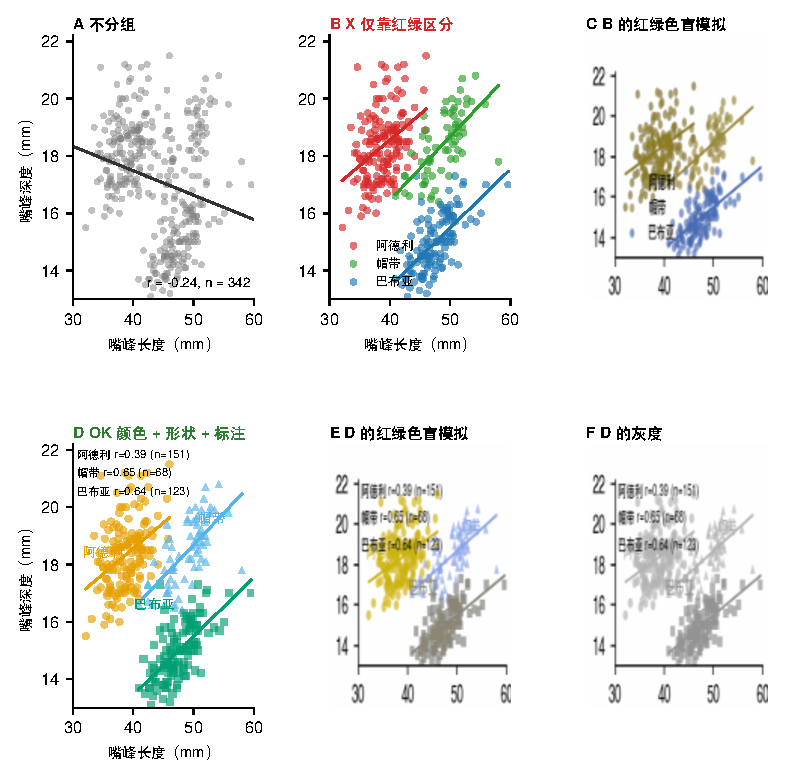
\includegraphics[width=\linewidth]{figures/ch05/ch05-08-scatter-cvd-zh.pdf}
\caption{分组改变相关方向，颜色必须经得起检查。企鹅嘴峰长度与深度（$n = 342$ 条记录）。A 全部记录合并时为负相关（$r = -0.24$）；B、D 按物种分组后三组均为正相关（$r = 0.39$、$0.65$、$0.64$）。B 只用红绿区分物种，在第二色盲模拟（C，Machado 等 2009 模型）下难以分辨；D 同时使用色觉友好配色、形状和直接标注，在模拟（E）和灰度（F）下仍可区分。直线为各组最小二乘拟合，仅作描述。}\label{fig:ch05-08}
\end{figure}

先对比图~\ref{fig:ch05-08} 的面板 A 与面板 D：
在\textbf{面板 A（不分组）}中，全部 342 条记录被混作一团灰点，普通最小二乘（OLS）线性拟合黑线明显向右下倾斜，皮尔逊相关系数为 $r = -0.24$（$n = 342$）。如果只看面板 A，就会得出“企鹅嘴峰越长、嘴峰越浅（负相关）”的错误结论。

再看\textbf{面板 B 与面板 D（按物种分组）}：一旦按物种把这 342 个点分开并各自拟合回归线，相关方向发生了 180 度反转！在每个物种内部，嘴峰长度与深度全部呈显著正相关：阿德利企鹅 $r = 0.39$（$n = 151$，左上橙色圆点），帽带企鹅 $r = 0.65$（$n = 68$，右上天蓝三角），巴布亚企鹅 $r = 0.64$（$n = 123$，下方蓝绿方块）。为什么合并后会变成负相关？从面板 D 的空间分布一眼就能看清：体型最大的巴布亚企鹅整体具有“长而相对较浅”的喙（集中在右下方），而阿德利企鹅具有“短而较深”的喙（集中在左上方）；而在每个物种内部，个体越大，喙既越长也越深。面板 A 的总回归线实际上是在连接不同物种团块的中心位置，把**物种间的形态分异**错当成了**物种内个体的长深关系**。

因此，指导 AI 绘制散点与相关图时必须守住三条原则：(1) 先交代物种、性别、站点等分组变量，绝不盲目画全体一条回归线；(2) 图上报告相关系数 $r$ 时必须同时写出样本量 $n$ 与分组层级（如面板 D 左上角），并在图注说明拟合方法；(3) 不在图上盲目堆砌简单线性回归的 $p$ 值。

\section{让图诚实：截断轴、3D、小数和彩虹色}

除了双纵轴，以下四类常见错误同样会破坏数据图的定量诚实性：\textbf{截断柱状图纵轴、3D 立体柱、伪精度的小数位，以及彩虹色图。}

图~\ref{fig:ch05-05} 用前文三种企鹅的体重均值数据（$n = 342$），并排对比了集中包含前三类错误的误导画法（左）与修改后的诚实点图（右）。

\begin{figure}[htbp]\centering
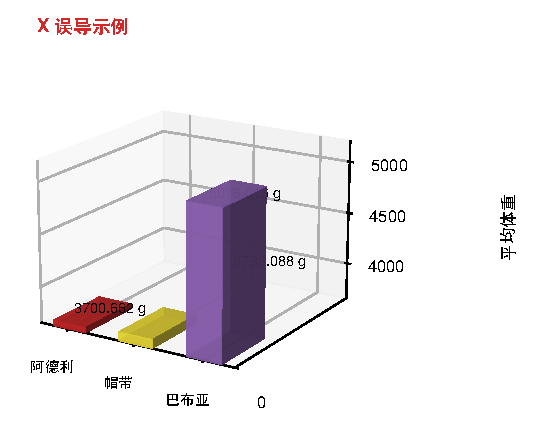
\includegraphics[width=0.49\linewidth]{figures/ch05/ch05-05-axis-bad-zh.pdf}\hfill
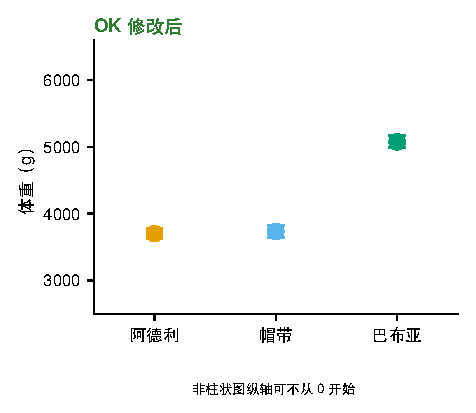
\includegraphics[width=0.49\linewidth]{figures/ch05/ch05-05-axis-good-zh.pdf}
\caption{同一组均值的误导画法与诚实画法（左为教学用错误示范）。左：3D 柱、纵轴从 $3650\ \text{g}$ 截断、彩虹配色、三位小数、缺少单位，使阿德利与帽带企鹅不足 1\% 的差异看起来像数倍差异。右：均值与 95\% 置信区间，纵轴有单位、刻度为整数。数据同图~\ref{fig:ch05-01}（$n = 342$）。}\label{fig:ch05-05}
\end{figure}

逐一剖析图~\ref{fig:ch05-05} 左图（\texttt{X 误导示例}）中的实际硬伤：
\begin{enumerate}
\item \textbf{截断柱状图纵轴夸大微小差异：}柱状图依赖**柱体距零基线的高度与面积**编码数值，纵轴必须从 $0$ 开始。左图将竖轴从 $3650\ \text{g}$ 截断起步：阿德利（$3700.7\ \text{g}$）与帽带（$3733.1\ \text{g}$）均值原本仅相差 $32.4\ \text{g}$（相对差异不足 $0.9\%$），减去 $3650\ \text{g}$ 基线后，红柱与黄柱的剩余高度变为 $50.7\ \text{g}$ 与 $83.1\ \text{g}$，视觉高度相差逾六成，而巴布亚（$5076.0\ \text{g}$）的紫柱更像高塔一样冲出视野。右图（\texttt{OK 修改后}）改用**均值点加 95\% 置信区间（点图）**：因为点图靠点在坐标轴上的位置而非柱体面积编码数值，纵轴可以从合理区间（$2500\text{--}6600\ \text{g}$）起步（图底专门注明“非柱状图纵轴可不从 0 开始”），前两个物种均值几乎齐平、置信区间大幅重叠的事实一目了然。
\item \textbf{3D 立体柱造成透视畸变与标签碰撞：}左图使用三维立体柱（\texttt{bar3d}），倾斜的柱顶让读者根本无法判断该拿前棱还是后棱去对齐右侧刻度（$4000, 4500, 5000$）；同时画面右下角多出无意义的纵深轴刻度“\texttt{0}”，右侧竖轴标题“平均体重”被挤到画幅边缘裁切不全，而半空中的数值标签 \texttt{5076.016 g} 与 \texttt{3733.088 g} 直接撞在紫色立体柱上。二维分组数据绝不应使用 3D 柱。
\item \textbf{多余小数位制造伪精度，且漏写单位：}野外称重最小刻度为 $25\ \text{g}$ 或 $50\ \text{g}$，左图却在柱顶标出毫克级的三位小数（\texttt{3700.662 g} 等）且竖轴无单位；右图删去图内冗余数字标签，纵轴规范标注“体重（g）”并采用整千刻度。
\end{enumerate}

第四类错误是连续矩阵与场数据中的\textbf{彩虹色图（\texttt{jet}）}。图~\ref{fig:ch05-07} 将 Mauna Loa 观测站 1959—2025 年共 67 个完整年 $\times$ 12 个月的 $\text{CO}_2$ 月均值排成 $67 \times 12$ 矩阵（不插值、不平滑，范围 $312.42\text{--}432.34\ \text{ppm}$），对比了 \texttt{jet} 彩虹色图与感知均匀色图 \texttt{viridis}。

\begin{figure}[htbp]\centering
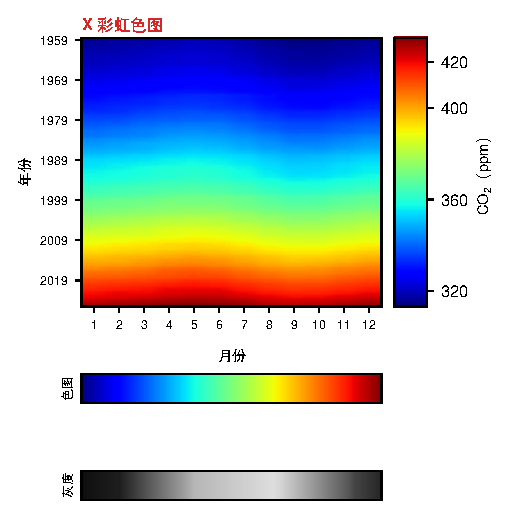
\includegraphics[width=0.49\linewidth]{figures/ch05/ch05-07-colormap-bad-zh.pdf}\hfill
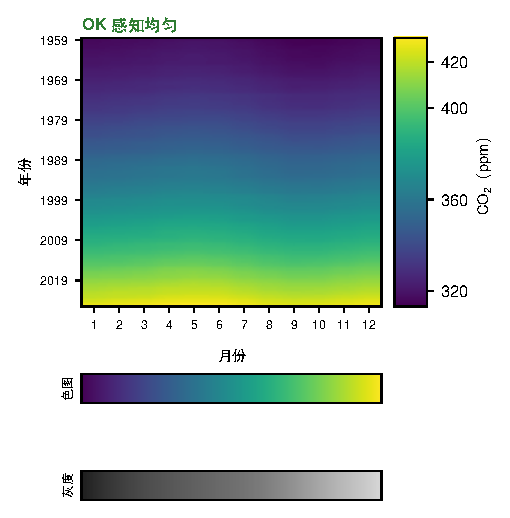
\includegraphics[width=0.49\linewidth]{figures/ch05/ch05-07-colormap-good-zh.pdf}
\caption{彩虹色图与感知均匀色图（左为教学用错误示范）。两张热图使用同一矩阵：Mauna Loa 1959—2025 年每月 $\text{CO}_2$ 均值。左 \texttt{jet} 色图在青、黄处出现数据中并不存在的“边界”，其灰度条亮度先升后降；右 \texttt{viridis} 的亮度单调上升，灰度打印后仍能读出高低顺序。}\label{fig:ch05-07}
\end{figure}

对比图~\ref{fig:ch05-07} 的左右两图及底部窄条可以看到：虽然 67 年来 $\text{CO}_2$ 浓度平稳上升，左图（\texttt{X 彩虹色图}）却在 1989 年前后的亮青色带和 2009 年前后的亮黄色带处造出两条刺眼的“假边界”；更严重的是，底部“灰度”转换条显示 \texttt{jet} 的感知亮度先升后降、两端（深蓝与深红）全暗，黑白打印后低值与高值混为一谈（Crameri 等，2020；Nuñez 等，2018）。右图（\texttt{OK 感知均匀}）改用 \texttt{viridis}（或针对重度色觉缺陷优化的 \texttt{cividis}），其灰度条从左至右单调变亮，既无假边界，黑白打印下也能准确读出长期上升与每年 5 月偏亮、9—10 月偏暗的季节波动。

在 \sdtool{sci-vis} 中遇到上述问题时，可直接发送如下修改指令：

\begin{Prompt}
1. 改为平面二维均值点 + 95% 置信区间图（若用柱状图，纵轴必须从 0 开始）；
   严禁使用 3D 立体柱；去掉三位小数标签，纵轴标题写为“体重（g）”，使用整数刻度。
2. 热图色图请将 jet 改为感知均匀的 viridis（或 cividis），色标注明单位“CO2（ppm）”。
\end{Prompt}

\section{色觉与灰度检查}

在北欧血统男性中约 8\% 有某种红绿色觉异常（最常见为第二色盲或绿色弱），其他人群中也有相当比例的读者受此影响（Wong，2011），加上黑白打印阅读场景，分组图绝不能只靠红绿颜色区分。

回到图~\ref{fig:ch05-08} 的面板 B–F：\textbf{面板 B} 将三个物种全部画成同样大小的实心圆点，仅靠红、绿、蓝三色区分；经基于生理学的色觉缺陷模型（Machado 等，2009）做第二色盲（deuteranopia）模拟后（\textbf{面板 C}），红色的阿德利点云与绿色的帽带点云连同各自的回归线、图例圆点一起塌缩成了难以分辨的黄褐色。相反，\textbf{面板 D} 同时采取三项措施：(1) 换用 Okabe–Ito 色觉安全配色（橙 \texttt{\#E69F00}、天蓝 \texttt{\#56B4E9}、蓝绿 \texttt{\#009E73}）；(2) 引入\textbf{形状冗余编码}（阿德利圆点 \texttt{o}、帽带三角形 \texttt{\^{}}、巴布亚正方形 \texttt{s}）；(3) 在各点云旁\textbf{直接标注物种名称}（实际排版时还应在终尺寸下检查标签位置，如面板 D 左上角相关系数文字紧邻高处散点、“巴布亚”贴近点云上沿，必要时可微调留白以免压点）。凭借这三重设计，无论在第二色盲模拟（\textbf{面板 E}）还是 CIELAB 亮度灰度图（\textbf{面板 F}）下，三个物种的点云与拟合线依然一目了然。

日常作图时，可将导出的图片上传至 \scidraw{} 图片检查（\sdtool{figure-checker}），一键完成灰度转换与色觉模拟检查；但须记住该工具仅覆盖技术检查，不能替代作者对科学逻辑（如面板 A 的辛普森悖论）的审核。

\section{贯穿案例：用 SciDraw AI 完成一张企鹅体重图}

现在我们把全章原则串联起来，完成开篇林悦的任务：基于公开数据集 \path{penguins.csv}，在论文“研究对象”一节和组会幻灯片中展示三种 \emph{Pygoscelis} 企鹅（阿德利 \emph{P.\ adeliae}、帽带 \emph{P.\ antarcticus}、巴布亚 \emph{P.\ papua}）繁殖成体的体重分布，以及每个物种内部雌雄体重的差别。明确科学边界：\textbf{本图仅作描述性形态展示，不做任何推断统计检验，不画星号或 $p$ 值。}

\textbf{第一步：独立复算期望值（准备核验标尺）。}按表~\ref{tab:ch05-dict} 规则，剔除 \texttt{sex} 或 \texttt{body\_mass\_g} 为 \texttt{NA} 的 11 行后保留 \textbf{$n = 333$} 行。在把数据交给 AI 之前，先用简单脚本或电子表格算出 6 个交叉子组的统计量（表~\ref{tab:ch05-case-expect}，SD 采用样本标准差 $\text{ddof}=1$；仅按物种合并的汇总量见前文表~\ref{tab:ch05-err}）。对比两表可见，分开雌雄后，每个物种内雄性均值都比雌性重 $412\text{--}805\ \text{g}$，且各亚组内的 SD（$269.4\text{--}362.1\ \text{g}$）比合并性别时的 SD（$384.3\text{--}504.1\ \text{g}$）明显缩小——说明原先混合分布的很大一部分离散度正是性别二态性造成的。

\begin{table}[htbp]\centering\footnotesize
\setlength{\tabcolsep}{4pt}
\renewcommand{\arraystretch}{1.15}
\caption{企鹅体重按“物种 $\times$ 性别”分组的核验期望值表（剔除缺失 11 行后，$n = 333$）。}\label{tab:ch05-case-expect}
\begin{tabularx}{\linewidth}{@{}llccY@{}}
\toprule
\textbf{物种（中文 / 英文与学名）} & \textbf{性别} & \textbf{记录数 $n$} & \textbf{均值 (g)} & \textbf{样本标准差 SD (g)} \\
\midrule
阿德利（Adelie, \emph{P.\ adeliae}） & 雌（female） & 73 & 3368.8 & 269.4 \\
阿德利（Adelie, \emph{P.\ adeliae}） & 雄（male）   & 73 & 4043.5 & 346.8 \\
帽带（Chinstrap, \emph{P.\ antarcticus}） & 雌（female） & 34 & 3527.2 & 285.3 \\
帽带（Chinstrap, \emph{P.\ antarcticus}） & 雄（male）   & 34 & 3939.0 & 362.1 \\
巴布亚（Gentoo, \emph{P.\ papua}） & 雌（female） & 58 & 4679.7 & 281.6 \\
巴布亚（Gentoo, \emph{P.\ papua}） & 雄（male）   & 61 & 5484.8 & 313.2 \\
\bottomrule
\end{tabularx}
\end{table}

\textbf{第二步：编写任务书并按向导进入绘图。}先把下面的任务书保存在自己的文档里；再打开 \scidraw{} 科研绘图向导（\sdtool{figure-workflow}），选“数据图”，从第 1 步“上传数据并绘图”进入科学可视化（\sdtool{sci-vis}）：

\begin{Prompt}
【研究问题】三种 Pygoscelis 企鹅的体重分布有何不同？每个物种内，雌雄体重相差多少？
【用途与读者】论文“研究对象”一节的描述性图 + 组会幻灯片；读者为生态学同行。
             单栏宽约 85 mm；同一张图另存一版供幻灯片使用。
【数据来源】真实公开数据：palmerpenguins v0.1.0 的 penguins.csv（CC0），
             Palmer Station LTER，2007–2009。
【字段与单位】species（分组）、sex（分组）、body_mass_g（体重，g）。其余列本图不用。
【观测单位与样本量】每行是一条测量记录。剔除 sex 或 body_mass_g 为 NA 的行（共 11 行），
             保留 333 行。每组 n 必须在图上可见。
【配对关系】无。不同记录之间不配对，不要连线。
【希望表达】分布与比较：每个物种内雌雄并排；物种按 Adelie、Chinstrap、Gentoo 排列。
【汇总与误差条】显示全部原始点（只在横向抖动，纵向值不变）；每组叠加均值 ± 1 SD。
             不做显著性检验，不画星号或 p 值。
【不允许的处理】不编造、删除或静默修改任何数值；不剔除“离群值”；不插补缺失值。
【标签与输出】纵轴“体重（g）”，整数刻度；横轴为物种；性别用空心/实心标记区分，
             颜色区分物种并对色觉异常友好；图例写明“均值 ± SD”。输出 PNG 和 PDF。
【验收】六组 n 依次为 73、73、34、34、58、61；六个均值与我核对的数值表一致（见数据字典附表）。
\end{Prompt}

\textbf{第三步：上传数据与排查初稿问题。}在科学可视化（\sdtool{sci-vis}）上传 \path{penguins.csv}（支持 CSV、TSV、TXT、XLSX、XLS 与粘贴表格；Excel 只读首个工作表），首先核对界面显示的行列信息是否为 344 行 $\times$ 8 列。平台对上传数据做哈希、字节数与行数校验，并提供“下载原始数据”供取回比对，保证画的是你上传的那份数据；但这不证明统计选择正确。在“绘图要求”输入框粘贴任务书要求后生成初稿，对照表~\ref{tab:ch05-case-expect} 逐项排查五类常见初稿问题：(1) 画成均值柱 + 不明误差线（常为 SEM）；(2) 性别被合并，或 \texttt{sex} 为 \texttt{NA} 的记录被当作第三个性别组“\texttt{NA}”；(3) 柱状图纵轴从非零值截断；(4) 均值标签带 1–3 位小数；(5) 颜色为红/绿或默认彩色，未配空心/实心标记。

\textbf{第四步：分步下达修改指令与历史版本恢复。}在会话底部继续输入修改指令，一次只改一类问题。第一轮修改指令 M1（图型与数据清理）：

\begin{Prompt}
请改为散点图：每个点是一条测量记录，横轴为物种（Adelie、Chinstrap、Gentoo 依次排列），
每个物种内雌性在左、雄性在右。点只在横向轻微抖动（宽度不超过组间距的 15%），纵向数值不变。
剔除 sex 或 body_mass_g 为 NA 的行，不要出现“NA”组。不要画柱子。其余设置保持不变。
\end{Prompt}

第二轮修改指令 M2（汇总量与样本量标注）：

\begin{Prompt}
在每组点的右侧叠加均值（短横线）和均值 ± 1 个标准差（SD，样本标准差）的竖线。
在每组下方标注样本量，例如“n = 73”。图例中写明“横线：均值；竖线：± 1 SD”。
不要添加显著性星号、p 值或检验结果。只改这两项，其余保持不变。
\end{Prompt}

第三轮修改指令 M3（坐标轴、整数刻度与色觉友好配色）：

\begin{Prompt}
纵轴标题为“体重（g）”，范围 2500–6500，刻度间隔 500，刻度为整数，不显示小数。
物种颜色使用对色觉异常友好的配色：Adelie 橙 #E69F00，Chinstrap 天蓝 #56B4E9，
Gentoo 蓝绿 #009E73；雌性空心圆，雄性实心圆。不要改变物种顺序和任何数值。
\end{Prompt}

注意：对话式修改不能保证“锁定”未提及的元素。若执行 M3 后发现意外改变了物种排列顺序或点的位置，不要在错图上继续叠加修补，而应立即点击“恢复上一版”（界面提示“已恢复上一版。”，也可从侧栏“历史记录”选回上一版），再把 M3 拆成两条更窄的指令（先改坐标轴，确认无误后再改配色与标记）。每次修改后都必须重新检查原本没要求改的部分。

\textbf{第五步：终稿核验、图注与交付文件夹。}平台后台用声明式图表或 Python 两条路径绘图，当前界面不提供完整代码下载，且声明式路径下导出的 PDF/EPS 可能是栅格包装（不要直接称为可编辑矢量；部分常见图型可导出原生 Excel 图表）。因此，我们用独立脚本复算并绘制标准对照终稿（图~\ref{fig:ch05-02}），对照表~\ref{tab:ch05-case-expect} 逐项核验：横轴依次为阿德利、帽带、巴布亚，每物种内左雌（空心圆）右雄（实心圆），点仅横向抖动；每组点右侧黑色短横线与竖线准确对应均值 $\pm 1\ \text{SD}$；横轴物种名下方分两行标出样本量（上行对应左侧雌性组：$n = 73, 34, 58$；下行对应右侧雄性组：$n = 73, 34, 61$，合计 333，无 \texttt{NA} 组）。

\begin{figure}[htbp]\centering
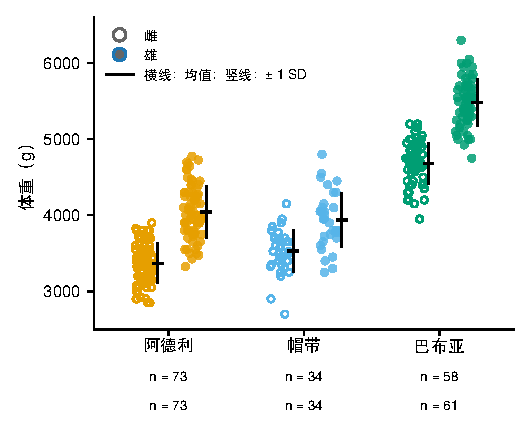
\includegraphics[width=0.68\linewidth]{figures/ch05/ch05-02-case-final-zh.pdf}
\caption{三种企鹅繁殖成体的体重（按物种与性别）。每个点为一条测量记录（Palmer Station LTER，2007—2009；palmerpenguins v0.1.0，CC0）。剔除性别或体重缺失的 11 条记录后 $n = 333$，各组 $n$ 标于横轴下方。横线为均值，竖线为均值 $\pm 1\ \text{SD}$（样本标准差）。点在横向随机抖动以减少重叠，纵向数值未改变。本图为描述性展示，未进行统计检验。}\label{fig:ch05-02}
\end{figure}

若把终稿交给 \sdtool{figure-legend} 起草图注，作者必须亲手补齐数据来源与许可、剔除 11 条缺失记录后的 $n = 333$、均值 $\pm 1\ \text{SD}$ 含义、“仅横向抖动”及“未进行统计检验”说明。最后将全套产物按如下结构归档交付（本章示例图由确定性脚本生成，提示词与核验记录见本书仓库）：

\begin{Prompt}
penguin-mass-figure/
  source/   penguins.csv、penguins-README.md、SHA-256.txt
  brief/    任务书.txt、数据字典.md、期望值表.csv
  drafts/   scivis-v1.png … scivis-v4.png、修改指令.md（每轮输入原文 + 发现的问题）
  check/    独立脚本复算输出 check.json、figure-checker 报告
  final/    figure-5-2.png、figure-5-2.pdf、图注-中.txt、caption-en.txt、AI 使用说明.txt
\end{Prompt}

\section{AI 在这一步能做什么与不能做什么}

表~\ref{tab:ch05-02} 汇总了数据可视化各环节中 AI 工具的能力边界与作者必须核对的事项。

\begin{table}[htbp]\centering\footnotesize
\setlength{\tabcolsep}{3pt}
\renewcommand{\arraystretch}{1.15}
\caption{数据可视化各环节中 AI 能做什么、不能做什么与作者要核对的内容。}\label{tab:ch05-02}
\begin{tabularx}{\linewidth}{@{}>{\raggedright\arraybackslash}p{18mm}YYY@{}}
\toprule
\textbf{环节} & \textbf{AI（\scidraw{} 科学可视化）能做} & \textbf{不能做 / 不应交给它} & \textbf{作者要核对} \\
\midrule
读取数据 & 解析 CSV、TSV、TXT、XLSX、XLS 与粘贴表格；校验上传数据的哈希、字节数与行数 & 知道哪一行属于同一个体、哪一列是配对键；判断缺失值的原因；Excel 只读首个工作表 & 行数、列名、NA 数与原始文件一致；观测单位写进任务书 \\
选择图型 & 按指令画散点、箱线、点线、折线、热图等；根据描述提出候选 & 理解研究设计（独立/配对/重复测量）除非你写明；当前界面不展示图型推荐理由 & 图型与研究设计匹配；全部原始点是否需要显示 \\
汇总与误差线 & 计算均值、SD、SEM、CI 并画出 & 替你决定该用哪种误差线；保证统计检验适用 & 误差线类型写在图例和图注；$n$ 与图上一致；无未要求的星号/$p$ 值 \\
多轮修改 & 在会话中按指令改图型、标签、颜色、轴；从历史图继续；恢复上一版 & 保证只改你要求的部分；“锁定”某个元素 & 每轮修改后重新检查没要求改的部分（顺序、数值、范围） \\
颜色与可读性 & 应用指定调色板与期刊栏宽样式；图片检查中做灰度与色觉模拟 & 判断颜色是否承载了科学含义；技术检查不代表科学审核 & 色觉模拟/灰度下分组仍可区分；色图与数据类型（顺序/发散/分类）匹配 \\
导出 & 下载 PNG、TIFF、PDF、EPS；下载原始数据；部分图型导出原生 Excel 图表 & 当前界面不提供完整绘图代码下载；PDF/EPS 不一定是可编辑矢量 & 打开导出文件确认尺寸、字体和是否栅格；源数据哈希与本地一致 \\
图注 & \sdtool{figure-legend} 根据图片起草描述 & 知道 $n$、剔除规则、误差线含义、数据来源（它只读图片） & 补齐数据来源、$n$、缺失值处理、误差线类型、是否检验 \\
\bottomrule
\end{tabularx}
\end{table}

\section{本章检查清单}

\begin{itemize}
\item 每一行代表什么已写在任务书里；“记录数”和“个体数”没有混用。
\item 缺失值怎么处理写明了；图上没有“NA”组；剔除的行数写进图注。
\item 图型与研究设计匹配：配对数据保留配对，时间轴是连续数值，分组变量在图上可见。
\item $n \le$ 几十时显示全部原始点；抖动只在横向。
\item 误差线类型（SD / SEM / 95\% CI）写在图例或图注里，$n$ 与图一致。
\item 柱状图纵轴从 0 开始；非柱状图的纵轴范围有理由，且不夸大差异。
\item 没有双纵轴、3D 柱、伪精度的小数。
\item 连续数据用感知均匀色图；分组颜色经过色觉模拟和灰度检查，并有形状或标注冗余。
\item 图上所有数字已与独立复算（脚本或表格软件）对照。
\item 保存了：原始数据及其哈希、任务书、每轮指令与截图、终稿、图注、核对记录。
\item 模拟数据在图或图注中标为“模拟教学数据”。
\end{itemize}

\section{练习}

\begin{enumerate}
\item \textbf{读表与选图（纸笔）：}给出 Palmer Penguins 的 \texttt{flipper\_length\_mm} 与 \texttt{island}。写一份数据字典（含 NA 数），统计各岛的物种构成（Torgersen 52 条阿德利；Biscoe 44 条阿德利 + 124 条巴布亚；Dream 56 条阿德利 + 68 条帽带），判断“比较三个岛上的鳍肢长度”为什么会与物种混杂（巴布亚只在 Biscoe、帽带只在 Dream），并提出一个不误导的图（例如按岛分面、按物种着色）。
\item \textbf{\scidraw{} 实操：}在 \sdtool{sci-vis} 上传 \texttt{paired-example.csv}，先只输入“画一张前后比较图”，记录初稿；再用本章图~\ref{fig:ch05-03} 的思路，通过对话分别得到配对点线图与差值图（纵轴含 0），至少使用一次“恢复上一版”。提交：每轮输入原文、截图，以及一张核对表（8 个差值逐一核对，\texttt{SIM04} $= -1$）。
\item \textbf{改错：}用本章 $\text{CO}_2$ 快照，自己制作一张“彩虹色 + 双纵轴”的错误图，再写出三条可以直接发给 AI 的修改指令把它改正；说明你如何确认修改后数值没有变（例如对比年均值表）。
\end{enumerate}

\section*{参考文献}

\begin{itemize}
\item Allen M, Poggiali D, Whitaker K, Marshall TR, Kievit RA. Raincloud plots: a multi-platform tool for robust data visualization. \emph{Wellcome Open Research}. 2019;4:63. \url{https://doi.org/10.12688/wellcomeopenres.15191.1}
\item ColorBrewer 2.0: color advice for cartography and scientific visualization. \url{https://colorbrewer2.org/}
\item Crameri F, Shephard GE, Heron PJ. The misuse of colour in science communication. \emph{Nature Communications}. 2020;11:5444. \url{https://doi.org/10.1038/s41467-020-19160-7}
\item Cumming G, Fidler F, Vaux DL. Error bars in experimental biology. \emph{Journal of Cell Biology}. 2007;177(1):7--11. \url{https://doi.org/10.1083/jcb.200611141}
\item Gorman KB, Williams TD, Fraser WR. Ecological sexual dimorphism and environmental variability within a community of Antarctic penguins (genus \emph{Pygoscelis}). \emph{PLoS ONE}. 2014;9(3):e90081. \url{https://doi.org/10.1371/journal.pone.0090081}
\item Horst AM, Hill AP, Gorman KB. palmerpenguins: Palmer Archipelago (Antarctica) penguin data (v0.1.0) [R package]. Zenodo; 2020. \url{https://doi.org/10.5281/zenodo.3960218}
\item Keeling CD. The concentration and isotopic abundances of carbon dioxide in the atmosphere. \emph{Tellus}. 1960;12(2):200--203. \url{https://doi.org/10.3402/tellusa.v12i2.9366}
\item Krzywinski M, Altman N. Points of significance: error bars. \emph{Nature Methods}. 2013;10(10):921--922. \url{https://doi.org/10.1038/nmeth.2659}
\item Lan X, Keeling R. Trends in atmospheric carbon dioxide: Mauna Loa monthly mean data. NOAA Global Monitoring Laboratory and Scripps Institution of Oceanography. \url{https://gml.noaa.gov/ccgg/trends/data.html}
\item Machado GM, Oliveira MM, Fernandes LAF. A physiologically-based model for simulation of color vision deficiency. \emph{IEEE Transactions on Visualization and Computer Graphics}. 2009;15(6):1291--1298. \url{https://doi.org/10.1109/TVCG.2009.113}
\item Nu\~nez JR, Anderton CR, Renslow RS. Optimizing colormaps with consideration for color vision deficiency to enable accurate interpretation of scientific data. \emph{PLoS ONE}. 2018;13(7):e0199239. \url{https://doi.org/10.1371/journal.pone.0199239}
\item Okabe M, Ito K. Color Universal Design (CUD): how to make figures and presentations that are friendly to colorblind people. \url{https://jfly.uni-koeln.de/color/}
\item Rougier NP, Droettboom M, Bourne PE. Ten simple rules for better figures. \emph{PLoS Computational Biology}. 2014;10(9):e1003833. \url{https://doi.org/10.1371/journal.pcbi.1003833}
\item Weissgerber TL, Milic NM, Winham SJ, Garovic VD. Beyond bar and line graphs: time for a new data presentation paradigm. \emph{PLOS Biology}. 2015;13(4):e1002128. \url{https://doi.org/10.1371/journal.pbio.1002128}
\item Wong B. Points of view: color blindness. \emph{Nature Methods}. 2011;8(6):441. \url{https://doi.org/10.1038/nmeth.1618}
\end{itemize}

% TODO: 待补充 SciDraw AI 科学可视化（/sci-vis）实测界面与迭代截图（磁盘上暂未生成，故正文未插）：
% - figures/ch05/ch05-scivis-v1.png（/sci-vis 初稿截图）
% - figures/ch05/ch05-scivis-v2.png … ch05-scivis-v4.png（多轮对话修改与恢复上一版截图）

\chapter{方法图与实验流程图}

肿瘤免疫学方向的博士后小陈正在撰写一篇小鼠肺部炎症模型的单细胞转录组论文。论文的第一张图（Figure 1A）需要放一张实验与数据分析流程图，向熟悉分子生物学但未必跑过单细胞管线的同行交代清楚：对照与处理两组小鼠的肺组织怎样一步步变成最终注释好的细胞图谱。

小陈打开图像生成工具，输入了一句英文提示词（意为“创建一张专业、色彩丰富的单细胞 RNA 测序实验与数据分析流程图，从组织到细胞类型注释，横向 16:9”）：

\begin{Prompt}
Create a professional, colorful flowchart of a single-cell RNA sequencing experiment and
data analysis workflow, from tissue to cell type annotation. Landscape 16:9.
\end{Prompt}

不到一分钟，屏幕跳出了一张十一格彩色信息图（图~\ref{fig:ch06-01}）。画面上方挂着深蓝色总标题，湿实验和生物信息学分析分别配了醒目的渐变色横幅，培养管、微流控通道、测序仪、小提琴图和散点图一应俱全。

\begin{figure}[htbp]\centering
\begin{tikzpicture}
\definecolor{ChSixBad}{HTML}{C0392B}
\node[anchor=south west,inner sep=0] (img) at (0,0) {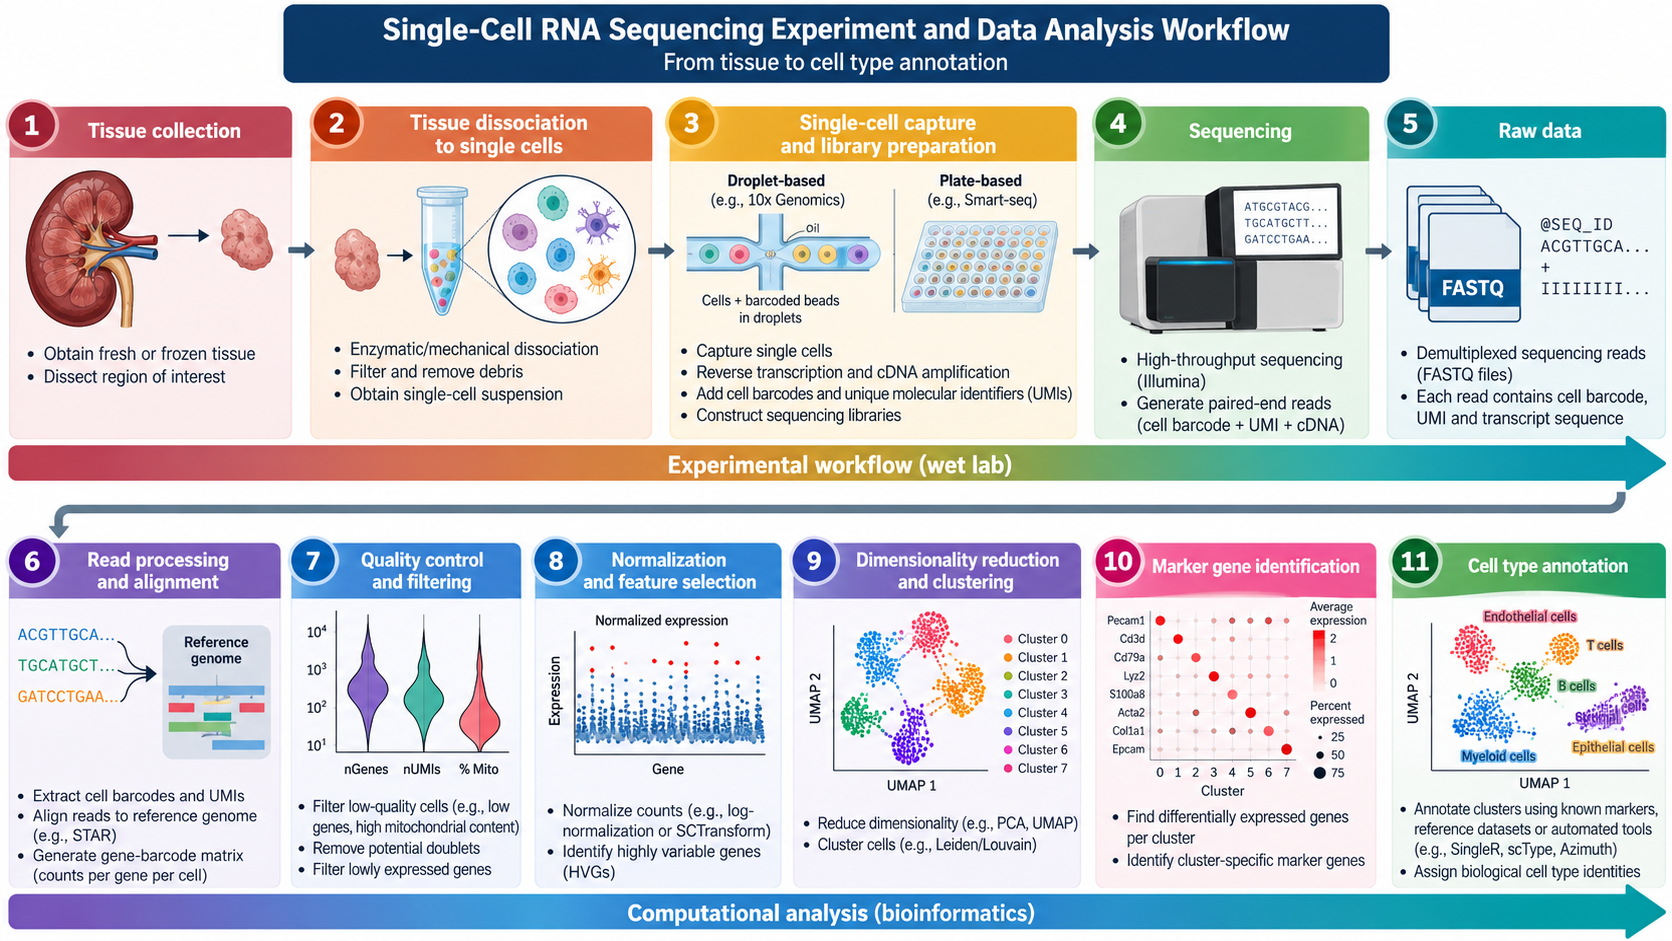
\includegraphics[width=\linewidth]{figures/ch06/ch06-01-v1-vague.png}};
\begin{scope}[x={(img.south east)},y={(img.north west)}]
  \tikzset{badmark/.style={draw=white,line width=0.8pt,fill=ChSixBad,text=white,circle,font=\sffamily\bfseries\scriptsize,inner sep=1.1pt,minimum size=4.2mm}}
  \node[badmark] at (0.09,0.74) {1};
  \node[badmark] at (0.36,0.80) {2};
  \node[badmark] at (0.91,0.78) {3};
  \node[badmark] at (0.24,0.36) {4};
  \node[badmark] at (0.55,0.36) {5};
  \node[badmark] at (0.91,0.28) {6};
\end{scope}
\end{tikzpicture}
\caption{只用一句话提示词生成的单细胞测序流程图初稿（教学用失败示例）。编号指出的问题：（1）左上画成单个肾脏，未体现对照与处理两份肺组织样本的并行处理；（2）湿实验缺少细胞活率与文库两道质控门，第 3 格同时塞入液滴法与孔板法并略去文库混合点；（3）第 5 格把数据产物 FASTQ 画成与测序同级的操作步骤；（4）第 7 格质控画成普通串联面板，没有通过与不通过两个出口；（5）第 9 格把降维、近邻图、聚类与 UMAP 笼统合为一格，看不出近邻图向聚类与可视化的分叉；（6）终点缺少异常簇返回复核的反馈回路，右下角“Stromal cells”标签直接压在紫色散点上，且全图文字锁死在位图中无法编辑。}\label{fig:ch06-01}
\end{figure}

然而把这张初稿放大到 200\% 逐格检查时，六处硬伤接连暴露（图~\ref{fig:ch06-01} 红圈 1–6）：左上角第 1 格画了一颗肾脏而非肺组织（因为提示词只写了泛泛的“tissue”），且全图只画了一条单样本路径，看不出对照组与处理组两个样本在哪里独立处理、在哪里混合测序；第 3 格把液滴法（10x Genomics）和孔板法（Smart-seq）两种实验路线并排塞进同一个步骤框，还将单细胞捕获、逆转录、cDNA 扩增与文库构建全部压成一个黑箱，中间既无细胞计数活率质控，也无文库片段质控；第 5 格把数据产物“Raw data（FASTQ）”画成了与“测序”同级的操作步骤框；下排第 7 格虽有小提琴图表示质控过滤，却只是普通串联面板，没有“合格放行、不合格排查”的出口；第 9 格把降维与聚类合画成一张带虚线圆圈的 UMAP 图，掩盖了“在主成分空间构建近邻图，再分别分叉去做聚类和 UMAP 展示”的分析拓扑；第 11 格注释终点不仅缺少发现低质量簇时退回上游的反馈路径，右下角“Stromal cells”字样还直接压在紫色细胞簇上，且高光阴影、渐变色带与大段说明文字全部锁死在位图里，缩排到期刊尺寸后既笨重又无法修改。

审稿人只需看五秒钟，就会发现图面与方法文字处处矛盾；小陈却在对话框里追着模型改了一下午，修好了器官图标，分支和箭头又乱了套。本章的办法是：\textbf{先把步骤写成表，再用确定性工具画结构骨架，最后才让 AI 负责图标与视觉风格。}

\section{流程图回答什么问题}

在科研论文里，方法图与实验流程图（workflow diagram）承担的任务和第 7 章要讨论的机制图截然不同。机制图回答的是“为什么会发生”——分子、细胞或组件之间通过什么因果作用产生效应；流程图回答的则是\textbf{“研究工作是怎么一步步做下来的”}——实验与计算包含哪些操作步骤，每一步接收什么输入、交出什么产物，在什么参数或质控条件下放行或退回，以及多份样本或多条计算支路在哪里分叉、在哪里汇合。

具体而言，一张结构清晰的流程图必须向读者交代清楚四个基本要素：
\begin{enumerate}
\item \textbf{步骤（做什么）：}对实验材料或数据集施加的具体操作，例如“组织解离”“文库构建”“比对与 UMI 计数”或“Leiden 聚类”。图中的每一个步骤框对应的都应当是一个明确的动作，而不是笼统的学科名词。
\item \textbf{产物（得到什么、交接什么）：}上一步操作结束时产生、并作为下一步输入的实体材料或数据对象，例如“单细胞悬液”“带条形码的 cDNA”“FASTQ 文件”或“过滤后计数矩阵”。在关键形态转换处把产物单独标出，读者才能看懂上下游步骤之间到底传递了什么。
\item \textbf{条件与质控（何时放行、何时返回）：}决定流程能否继续往下推进的实验参数与质量判断节点。凡是标为“质控”或“检查”的节点，在逻辑上都必然存在两种去向：合格时沿主干放行到下一步，不合格时沿反馈路径退回上游步骤重新优化、补样或调整过滤条件。
\item \textbf{分支与合并（谁和谁并行、在哪里汇合）：}真实的实验与计算流程很少是一根到底的直线。对照与处理样本往往先各自独立解离、捕获、建库，到上机测序前才按比例混合；计算分析中，主成分空间的近邻图既要送去运行图聚类算法以划分细胞亚群，又要送去计算二维嵌入坐标用于散点图展示。分叉点与合并点的位置直接反映了实验设计与分析逻辑。
\end{enumerate}

厘清这四个要素后，必须划定一条核心边界：\textbf{流程箭头只表示时间先后与物料或数据交接，不表示生物学因果、作用机制或效应大小。}例如在单细胞制备流程中，“组织解离 $\rightarrow$ 单细胞悬液”是一条标准的流程关系，表示前一步操作产出了后一件实验材料；但前人研究指出，较长时间的温热酶解离可能诱导部分组织亚群出现早期应激相关基因表达升高（van den Brink 等，2017）。后一句话属于实验操作引发的生物学效应或质控伪影提醒，如果用同一根实心流程箭头画成“组织解离 $\rightarrow$ 应激基因表达升高”，就会把实验操作步骤与细胞内在转录响应混为一谈。正确的处理方式是用浅灰色虚线引线把这类机制或质控背景写成旁注，或者直接交代在图注里。

为了防止读者在读图时靠猜来区分步骤、产物和判断条件，本书采用一套固定的流程图节点与箭头语法（图~\ref{fig:ch06-02}）。

\begin{figure}[htbp]\centering
% FIG ch06-02 flow grammar (Chinese)%
% Shared styles for chapter 6 workflow TikZ figures.%
% Every figure inputs this file, so commands are defined with \providecommand.%
\providecolor{BookTeal}{HTML}{176C68}%
\providecolor{BookInk}{HTML}{23363E}%
\providecolor{BookRule}{HTML}{C8D6D6}%
\providecolor{BookPale}{HTML}{F1F6F5}%
\definecolor{WetPale}{HTML}{FBF1EA}%
\definecolor{Wet}{HTML}{B5653A}%
\definecolor{Seq}{HTML}{8A6D1F}%
\definecolor{DryPale}{HTML}{EEF4F7}%
\definecolor{Dry}{HTML}{2F6F8F}%
\definecolor{ChSixFeedback}{HTML}{7A8A90}%
\definecolor{ChSixBad}{HTML}{C0392B}%
\usetikzlibrary{arrows.meta,positioning,shapes.geometric,shapes.misc,fit,backgrounds,calc}%
\ifdefined\ChSixLayersReady\else%
  \pgfdeclarelayer{chsixlane}%
  \pgfsetlayers{chsixlane,background,main}%
  \def\ChSixLayersReady{}%
\fi%

\tikzset{%
  chsix/.style={font=\sffamily\scriptsize, text=BookInk, align=center},%
  flowstep/.style={%
    chsix, rounded corners=2pt, draw=Wet, line width=0.45pt, fill=white,%
    text width=19mm, minimum height=7.4mm, inner sep=1.3pt,%
  },%
  flowstepdry/.style={flowstep, draw=Dry},%
  flowstepseq/.style={flowstep, draw=Seq},%
  artifact/.style={%
    chsix, trapezium, trapezium left angle=70, trapezium right angle=110,%
    trapezium stretches=true,%
    draw=BookInk, line width=0.45pt, fill=white,%
    minimum height=6.2mm, inner sep=1.2pt,%
  },%
  gate/.style={%
    chsix, diamond, aspect=1.7, draw=BookInk, line width=0.45pt, fill=white,%
    text width=12mm, inner sep=0.6pt, minimum height=8mm,%
  },%
  opt/.style={flowstep, dashed, draw=BookInk!70},%
  optdry/.style={flowstepdry, dashed, draw=BookInk!70},%
  stack/.style={flowstep},%
  link/.style={-{Stealth[length=1.6mm]}, semithick, draw=BookInk},%
  linkthin/.style={-{Stealth[length=1.2mm]}, thin, draw=BookInk!80},%
  back/.style={-{Stealth[length=1.5mm]}, dashed, draw=ChSixFeedback},%
  conn/.style={%
    circle, draw=BookInk, line width=0.5pt, minimum size=4.6mm,%
    font=\sffamily\scriptsize\bfseries, inner sep=0pt, text=BookInk,%
  },%
  lanetitle/.style={font=\sffamily\bfseries\small, text=BookInk, align=left},%
  passlabel/.style={font=\sffamily\scriptsize, text=BookInk, fill=white, inner sep=0.7pt, align=center},%
  mergelabel/.style={font=\sffamily\scriptsize, text=BookInk, fill=white, inner sep=0.8pt, align=center},%
  taglab/.style={font=\sffamily\scriptsize, text=ChSixFeedback, fill=white, inner sep=0.8pt, align=center},%
  gramcap/.style={font=\sffamily\scriptsize, text=BookInk, align=left, anchor=west},%
}%

% Offset card behind a two-sample step. Text stays on the front node only.%
\providecommand{\ChSixCardBack}[1]{%
  \begin{pgfonlayer}{background}%
    \draw[Wet, line width=0.45pt, rounded corners=2pt, fill=white]%
      ([shift={(-0.55mm,0.55mm)}]#1.south west)%
      rectangle ([shift={(-0.55mm,0.55mm)}]#1.north east);%
  \end{pgfonlayer}%
}%
% #1 options, #2 name, #3 position (with parentheses), #4 text%
\providecommand{\ChSixCard}[4]{%
  \node[stack, #1] (#2) at #3 {#4};%
  \ChSixCardBack{#2}%
}%

\providecommand{\ChSixMaybeLabel}[1]{%
  \ifdefined\nolabels\else#1\fi%
}%

\providecommand{\ChSixIcon}[2]{%
  \ifdefined\ChSixShowIcons%
    \IfFileExists{#1}{%
      \node[anchor=south, inner sep=0] at ([yshift=0.7mm]#2.north)%
        {\includegraphics[height=5.4mm]{#1}};%
    }{}%
  \fi%
}%
%
\begin{tikzpicture}[x=1mm, y=1mm, font=\sffamily\scriptsize, text=BookInk]%
  \node[anchor=north west, font=\sffamily\bfseries\small] (titleL) at (0,0) {节点与箭头语法};%
  \draw[BookRule, line width=0.4pt] (0,-7) rectangle (128,-126);%

  \node[flowstep] (g1) at (16,-14) {操作步骤};%
  \node[gramcap] at (36,-14) {圆角矩形——做什么};%

  \node[artifact] (g2) at (16,-25) {产物};%
  \node[gramcap] at (36,-25) {平行四边形——得到什么、交给下一步什么};%

  \node[gate] (g3) at (16,-38) {质控};%
  \node[passlabel, anchor=west] at ([xshift=1.5mm]g3.east) {通过};%
  \node[taglab, anchor=north west] at ([xshift=1.5mm, yshift=-0.6mm]g3.south east) {不通过};%
  \node[gramcap] at (36,-38) {菱形——须有两个出口（通过 / 不通过）};%

  \node[opt] (g4) at (16,-50) {可选步骤};%
  \node[gramcap] at (36,-50) {虚线圆角矩形};%

  \node[stack] (gs1) at (13,-61) {};%
  \ChSixCardBack{gs1}%
  \node[stack] (gs2) at (16.2,-61) {每样本};%
  \node[gramcap] at (36,-61) {错位叠放——每个样本分别进行};%

  \draw[link] (6,-72) -- ++(16,0);%
  \node[gramcap] at (36,-72) {实线箭头——顺序与交接};%

  \draw[back] (6,-83) to[out=20, in=160] (24,-83);%
  \node[gramcap] at (36,-83) {虚线弧——反馈或返回};%

  \fill (16,-94) circle (0.7pt);%
  \node[gramcap] at (36,-94) {实心圆点——分叉 / 合并点};%

  \node[conn] (gc) at (16,-105) {A};%
  \node[gramcap] at (36,-105) {圆形连接符——跨行续接};%

  \fill[WetPale, draw=Wet, line width=0.3pt] (6,-116) rectangle (16,-122);%
  \fill[DryPale, draw=Dry, line width=0.3pt] (18,-116) rectangle (28,-122);%
  \node[gramcap] at (36,-119) {泳道底色——湿实验 / 计算};%

  \node[anchor=north west, font=\sffamily\bfseries\small] (titleR) at (0,-130) {流程箭头 ≠ 因果};%
  \node[flowstep] (d1) at (18,-144) {组织解离};%
  \node[artifact] (d2) at (46,-144) {单细胞悬液};%
  \draw[link] (d1) -- (d2);%
  \node[gramcap] at (68,-144) {流程：先后与交接};%

  \node[flowstep] (e1) at (18,-160) {组织解离};%
  \node[gramcap] at (40,-160) {$\Rightarrow$ 应激相关基因表达升高};%
  \draw[BookInk!45, densely dotted] (e1.east) -- ++(6,0);%
  \node[gramcap, anchor=north west, text width=120mm] at (0,-170)%
    {机制或因果信息写成注释或图注，不画成流程箭头（van den Brink 等 2017）。};%
\end{tikzpicture}%

\caption{本书流程图使用的节点与箭头。每种形状只表示一种含义。下框：流程箭头表示先后与交接；解离可能诱导应激相关基因表达（van den Brink 等，2017）这类机制信息写成注释，不画成流程箭头。}\label{fig:ch06-02}
\end{figure}

如图~\ref{fig:ch06-02} 所示，这套语法遵循“一形一义”的视觉编码原则（Wong，2010；Wong，2011a）：
\begin{itemize}
\item \textbf{圆角矩形表示操作步骤：}框内写动宾短语或操作名称（如“组织解离”“PCA 降维”），不混写输入输出文件名。
\item \textbf{平行四边形表示数据或材料产物：}放在关键交接步骤之间或分支终点，标明交付的实物或数据结构（如“单细胞悬液”“原始计数矩阵”）。
\item \textbf{菱形表示质控或条件判断：}每一个菱形节点都必须同时画出“通过”和“不通过”两个出口。
\item \textbf{虚线圆角矩形表示可选步骤：}用于标记随具体组织类型、实验设计或软件路线而异的操作（如“红细胞裂解”“批次整合”）。
\item \textbf{错位叠放的双层圆角矩形表示多样本分别进行：}当对照组与处理组样本按完全相同的规程各自独立完成某一步时，用两张轻微错位叠放的卡片表示“每个样本分别进行”，既省去重复画两条平行长链的版面开销，又比单层方框多传递了样本独立性信息。
\item \textbf{实线箭头与虚线弧区分顺向交接与反馈迭代：}深灰实线配实心三角箭头专用于顺向交接；中灰虚线弧专用于质控未通过或下游结果异常时向上游步骤的返回与迭代。
\item \textbf{实心圆点、圆形连接符与泳道色带组织宏观版面：}分叉与合并处点一枚实心小圆点；跨行或跨泳道续接时使用写有同一字母的圆形连接符（如“A”）；全图背景按阶段铺设浅暖色（湿实验与测序）与浅冷色（计算分析）两条水平泳道色带，并在左上角配粗体泳道标题，确保即使灰度打印也能一眼分清实验台操作与计算机分析。
\end{itemize}

\section{从方法记录到步骤表}

为什么把论文方法部分的文字直接贴给 AI，往往画不出合格的流程图？因为论文方法章节是按\textbf{文字叙述顺序}组织的，而流程图必须按\textbf{输入与产物的交接关系}组织。

在文字段落里，作者常把同类概念合在一起写，或者用“随后”“同时”“必要时”一笔带过分支条件；可是一旦落到图纸上，每一个框连向哪里、两条线在哪个节点汇合，都必须有唯一确定的答案。因此，从方法记录走向流程图的第一步，不是构思配色和图标，而是把叙述文字拆解成一张结构化的\textbf{步骤表}。

下面以本章主案例——比较对照与处理两种条件下小鼠肺组织细胞组成的微滴法 3$'$ 端单细胞 RNA 测序流程——演示这一转换过程。本案例的实验与分析步骤依据单细胞测序领域的通用规程与综述整理：液滴捕获、细胞条形码（cell barcode）与唯一分子标识符（UMI）原理参照 Islam 等（2014）、Macosko 等（2015）、Zheng 等（2017）及 Hwang 等（2018）；计算质控、标准化、高变基因选择、降维、近邻图、聚类与细胞类型注释流程参照 Wolf 等（2018）、Luecken 与 Theis（2019）及 Heumos 等（2023）；Leiden 聚类算法参照 Traag 等（2019）；双细胞检测与环境游离 RNA 校正分别参照 Wolock 等（2019）与 Young 和 Behjati（2020）。

需要明说的是，下面这段材料是本书编写的\textbf{教学用方法记录}，按上述通用流程组织，不对应任何具体论文的真实测量，因此凡涉及酶浓度、消化时间、活率阈值或过滤阈值的参数，一律写成“〔作者填写〕”：

\begin{BookNote}
对照与处理组小鼠各取肺组织一份，分别处理。组织剪碎后在〔酶与浓度〕中于〔温度〕消化〔时间〕，期间机械吹打；经〔孔径〕细胞筛过滤，〔可选：红细胞裂解；死细胞去除〕。用〔方法〕计数并评估活率，活率低于〔阈值〕时重新优化解离。合格的单细胞悬液按〔目标细胞数〕上样到微流控芯片，细胞与带条形码的凝胶珠共同包裹在油包水微滴中；微滴内细胞裂解，mRNA 经含细胞条形码、UMI 与 poly(dT) 的引物逆转录。破乳后纯化并扩增 cDNA，检测片段分布。cDNA 经片段化、末端修复与加 A、接头连接和样本索引 PCR 构建文库，检测文库片段大小与浓度后，两个样本的文库按〔比例〕混合，在〔测序平台〕上双端测序（Read 1：细胞条形码 + UMI；Read 2：cDNA 片段）。

测序数据拆分为 FASTQ 后，比对到〔参考基因组版本〕并按 UMI 计数，得到每个样本的基因 $\times$ 条形码矩阵；识别含细胞的条形码，按 UMI 总数、检测基因数和线粒体基因读段比例过滤低质量细胞（阈值〔作者依分布确定〕），同时进行双细胞检测与环境 RNA 校正（可选）。两样本合并后进行文库大小标准化与对数转换，选择高变基因，PCA 降维（如有批次效应则整合），构建 $k$ 近邻图，在图上用 Leiden 算法聚类，并计算 UMAP 用于可视化。对每个簇找标志基因，结合已知标志物与参考数据集注释细胞类型；若出现低质量簇或分辨率不当，返回调整质控阈值或聚类分辨率。
\end{BookNote}

我们可以先让对话式 AI 从这段方法文字中抽出候选步骤行、提示可能遗漏的中间产物与质控口，但作者必须紧握两条主审原则：第一，\textbf{AI 不得编造任何实验参数或质控阈值}。大语言模型在整理方法表时，极易顺手补出看起来合理的温度、消化时长、活率百分比或线粒体比例阈值——这些数字必须全部标为“待确认”，由作者对照原始实验本与分析脚本亲自填写。第二，\textbf{每一步占一行，明确写出步骤编号、泳道、输入、产物、关键条件、质控出口与下游编号}。整理核实后的步骤表见表~\ref{tab:ch06-01}，它是本章绘图与核验的“唯一事实来源”。

\begin{table}[htbp]\centering\scriptsize
\setlength{\tabcolsep}{2pt}
\renewcommand{\arraystretch}{1.08}
\caption{液滴法单细胞 RNA 测序实验与分析流程步骤表（绘图的唯一事实来源）。}\label{tab:ch06-01}
\begin{tabularx}{\linewidth}{@{}l>{\raggedright\arraybackslash}p{15mm}l>{\raggedright\arraybackslash}p{16mm}>{\raggedright\arraybackslash}p{16mm}YYl@{}}
\toprule
\textbf{ID} & \textbf{步骤} & \textbf{泳道} & \textbf{输入} & \textbf{产物} & \textbf{关键条件（作者填写）} & \textbf{质控/判断与可选分支} & \textbf{下游} \\
\midrule
W1 & 组织采集 & 湿实验 & 小鼠（对照、处理） & 新鲜肺组织 & 采样时间、保存方式 & 两样本分别进行 & W2 \\
W2 & 组织解离 & 湿实验 & 肺组织 & 细胞悬液（粗） & 酶、浓度、温度、时间、机械方式 & 两样本分别进行 & W3 \\
W3 & 过滤与清洗 & 湿实验 & 粗悬液 & 单细胞悬液 & 筛孔径 & 可选 W3a 红细胞裂解、W3b 死细胞去除（虚线框） & Q1 \\
Q1 & 细胞计数与活率 & 湿实验 & 单细胞悬液 & 计数、活率记录 & 计数方法、活率阈值 & 通过 $\rightarrow$ W4；不通过 $\rightarrow$ 返回 W2（反馈弧） & W4 \\
W4 & 微滴捕获与条形码标记 & 湿实验 & 单细胞悬液、凝胶珠、油 & 微滴（每滴$\approx$一细胞一珠） & 目标细胞数、芯片类型 & 两样本分别上样 & W5 \\
W5 & 微滴内逆转录；破乳；cDNA 扩增 & 湿实验 & 微滴 & 带条形码的 cDNA & 扩增循环数 & cDNA 片段分布（记录，不设分支） & W6 \\
W6 & 文库构建 & 湿实验 & cDNA & 测序文库（每样本一索引） & 片段化、接头、索引 PCR 循环数 & 两样本分别建库 & Q2 \\
Q2 & 文库质控 & 湿实验 & 测序文库 & 片段大小、浓度记录 & 方法、合格标准 & 通过 $\rightarrow$ S1；不通过 $\rightarrow$ 返回 W6 & S1 \\
S1 & 文库混合与测序 & 湿实验（测序） & \textbf{两个样本的文库}（合并点） & 原始读段 $\rightarrow$ FASTQ & 平台、读长、测序深度 & 经连接符 A 交接至计算泳道 & C1 \\
C1 & 比对与 UMI 计数 & 计算 & FASTQ、参考基因组与注释 & 原始计数矩阵（每样本） & 软件与版本、参考版本 & 按样本分别比对计数 & C2 \\
C2 & 细胞识别 & 计算 & 原始计数矩阵 & 含细胞的条形码 & 方法 & 区分含细胞微滴与空滴 & Q3 \\
Q3 & 细胞级质控 & 计算 & 细胞矩阵 & 过滤后矩阵 & UMI 数、基因数、线粒体比例阈值 & 并行可选：C3a 双细胞检测 $\parallel$ C3b 环境 RNA 校正 & C4 \\
C4 & 合并样本；标准化与对数转换 & 计算 & \textbf{两样本过滤后矩阵}（合并点） & 标准化表达矩阵 & 方法 & 两样本矩阵在此合并 & C5 \\
C5 & 选择高变基因 & 计算 & 标准化矩阵 & 高变基因列表 & 基因数 & — & C6 \\
C6 & PCA 降维 & 计算 & 高变基因表达 & 主成分坐标 & 主成分数 & 可选 C6a 整合/批次校正（虚线框） & C7 \\
C7 & 构建 $k$ 近邻图 & 计算 & 主成分坐标 & 近邻图 & $k$ 值 & \textbf{分叉} $\rightarrow$ C8 与 C9 & C8、C9 \\
C8 & 聚类（Leiden） & 计算 & 近邻图 & 簇标签 & 分辨率 & — & C10 \\
C9 & UMAP 嵌入 & 计算 & 近邻图 & 二维坐标（\textbf{仅用于展示}） & 参数 & 终点，不连向 C8 或 C11 & （展示） \\
C10 & 标志基因分析 & 计算 & 标准化矩阵 + 簇标签 & 每簇标志基因表 & 检验方法 & — & C11 \\
C11 & 细胞类型注释 & 计算 & 标志基因表、标志物、参考集 & 注释后的细胞图谱 & 参考数据集版本 & 发现低质量簇/分辨率不当 $\rightarrow$ 返回 Q3 或 C8 & 终点 \\
\bottomrule
\end{tabularx}
\end{table}

细读表~\ref{tab:ch06-01}，它在动笔前帮作者理清了五个极易在画图时出错的方法学细节：
\begin{enumerate}
\item \textbf{两处合并点的位置不同：}湿实验中，对照与处理两个样本从 W1 到 Q2 各自独立处理，加上不同样本索引（sample index）后在 S1（文库混合与测序）处第一次合池测序；计算分析中，下机 FASTQ 按索引拆分后，仍先按样本分别比对计数（C1）、识别含细胞条形码（C2）并执行细胞级质控（Q3），直到 C4（合并与标准化）才将两个样本的过滤后矩阵合并。
\item \textbf{微滴内操作与破乳后扩增：}在 3$'$ 端液滴平台的一般流程中，微滴内部完成的是细胞裂解与 mRNA 逆转录，而 cDNA 扩增是在破乳纯化之后进行的。由于不同化学版本的具体细节略有差异，表~\ref{tab:ch06-01} 将“微滴内逆转录、破乳与 cDNA 扩增”合记为 W5，避开版本差异。
\item \textbf{理想化微滴示意与计算去噪的呼应：}W4 的图标通常画成“每滴含一个细胞与一颗凝胶珠”的理想化状态；但实际微流控上样时，为控制多细胞共包裹率，多数微滴为空滴（含环境游离 RNA），少数微滴含两个及以上细胞（双细胞）。这也正是计算泳道必须设置 C2 细胞识别、C3a 双细胞检测与 C3b 环境 RNA 校正的原因。
\item \textbf{可选步骤与整合位置：}不同分析软件中“整合/批次校正”所处的位置不同（本表放在 C6 PCA 降维之后作为虚线可选框 C6a，代表在主成分空间整合的方法；也有方法在标准化或特征选择阶段整合）；同样，C3a 双细胞检测与 C3b 环境 RNA 校正在不同管线中的先后关系不同，本表画成 Q3 下的并行可选分支，并在图注中明确声明这是教学简化。
\item \textbf{C7 处的平行分叉：}C7（$k$ 近邻图）分叉出 C8（Leiden 聚类）与 C9（UMAP 嵌入），C9 不连向 C8 或 C11。作者若确实把簇标签投射到 UMAP 图上辅助人工检查注释，可在图注中写“UMAP 用于展示与检查”，图中不画依赖箭头。
\end{enumerate}

由 AI 协助起草步骤表后，作者必须对照实验本与分析脚本逐项勾选表~\ref{tab:ch06-02} 的九项确认清单。凡是实际实验中没有做的可选步骤（如未做红细胞裂解或死细胞去除），在正式论文配图中应直接删掉虚线框，不保留“可能做过”的模糊表述。

\begin{table}[htbp]\centering\footnotesize
\setlength{\tabcolsep}{4pt}
\renewcommand{\arraystretch}{1.15}
\caption{作者确认清单（AI 起草步骤表后必须由作者逐项勾选）。}\label{tab:ch06-02}
\begin{tabularx}{\linewidth}{@{}c>{\raggedright\arraybackslash}p{28mm}Y@{}}
\toprule
\textbf{序号} & \textbf{核对维度} & \textbf{必须由作者对照原始实验记录或分析代码确认的具体事项} \\
\midrule
1 & 样本批次与通道 & 两个样本是否在同一批次、同一张芯片的不同通道处理？（决定是否画 C6a“整合”可选框） \\
2 & 湿实验可选步骤 & 是否实际做了 W3a 红细胞裂解、W3b 死细胞去除？未做就删掉虚线框，而不是保留“可能做过”。 \\
3 & 湿实验质控去向 & Q1、Q2 的合格标准和“不通过”的实际处理方式（返回优化、补样，还是终止）。 \\
4 & 测序读长结构 & 测序平台及双端读长结构（Read 1 / Read 2 各含什么序列）是否与所用试剂说明书一致。 \\
5 & 比对与参考版本 & C1 比对计数软件名称与版本、参考基因组与基因注释的具体版本。 \\
6 & 细胞质控与去噪 & Q3 的三个过滤阈值是否按数据分布确定、是否每个样本分别设定；C3a、C3b 是否真的做了。 \\
7 & 聚类空间来源 & C8 聚类所用的近邻图来自 PCA（或整合后的低维空间），而不是二维 UMAP 空间。 \\
8 & 细胞注释依据 & C11 注释依据（标志基因列表、参考数据集版本）以及是否有研究者人工复核。 \\
9 & 表图双向闭环 & 图中每个框都能在表~\ref{tab:ch06-01} 中找到对应行；表中每行都在图中出现或在图注中声明省略。 \\
\bottomrule
\end{tabularx}
\end{table}

\section{结构先行：用确定性工具画骨架}

拿到核实无误的步骤表后，为什么不直接把步骤表喂给图像生成模型出整图？

因为\textbf{图像生成模型在像素层面“画得像”，但不保证箭头数量、方向和连接对象正确}；而结构错误恰恰是流程图最致命的错误。最稳妥的做法是“结构先行”：先用确定性绘图工具（TikZ、PowerPoint、draw.io 或 Illustrator 等任何能对齐节点与连接线的工具）严格按表~\ref{tab:ch06-01} 画出\textbf{结构骨架图}（图~\ref{fig:ch06-03}）。

\begin{figure}[htbp]\centering
\resizebox{\linewidth}{!}{% FIG ch06-03 skeleton (Chinese)%
% Shared styles for chapter 6 workflow TikZ figures.%
% Every figure inputs this file, so commands are defined with \providecommand.%
\providecolor{BookTeal}{HTML}{176C68}%
\providecolor{BookInk}{HTML}{23363E}%
\providecolor{BookRule}{HTML}{C8D6D6}%
\providecolor{BookPale}{HTML}{F1F6F5}%
\definecolor{WetPale}{HTML}{FBF1EA}%
\definecolor{Wet}{HTML}{B5653A}%
\definecolor{Seq}{HTML}{8A6D1F}%
\definecolor{DryPale}{HTML}{EEF4F7}%
\definecolor{Dry}{HTML}{2F6F8F}%
\definecolor{ChSixFeedback}{HTML}{7A8A90}%
\definecolor{ChSixBad}{HTML}{C0392B}%
\usetikzlibrary{arrows.meta,positioning,shapes.geometric,shapes.misc,fit,backgrounds,calc}%
\ifdefined\ChSixLayersReady\else%
  \pgfdeclarelayer{chsixlane}%
  \pgfsetlayers{chsixlane,background,main}%
  \def\ChSixLayersReady{}%
\fi%

\tikzset{%
  chsix/.style={font=\sffamily\scriptsize, text=BookInk, align=center},%
  flowstep/.style={%
    chsix, rounded corners=2pt, draw=Wet, line width=0.45pt, fill=white,%
    text width=19mm, minimum height=7.4mm, inner sep=1.3pt,%
  },%
  flowstepdry/.style={flowstep, draw=Dry},%
  flowstepseq/.style={flowstep, draw=Seq},%
  artifact/.style={%
    chsix, trapezium, trapezium left angle=70, trapezium right angle=110,%
    trapezium stretches=true,%
    draw=BookInk, line width=0.45pt, fill=white,%
    minimum height=6.2mm, inner sep=1.2pt,%
  },%
  gate/.style={%
    chsix, diamond, aspect=1.7, draw=BookInk, line width=0.45pt, fill=white,%
    text width=12mm, inner sep=0.6pt, minimum height=8mm,%
  },%
  opt/.style={flowstep, dashed, draw=BookInk!70},%
  optdry/.style={flowstepdry, dashed, draw=BookInk!70},%
  stack/.style={flowstep},%
  link/.style={-{Stealth[length=1.6mm]}, semithick, draw=BookInk},%
  linkthin/.style={-{Stealth[length=1.2mm]}, thin, draw=BookInk!80},%
  back/.style={-{Stealth[length=1.5mm]}, dashed, draw=ChSixFeedback},%
  conn/.style={%
    circle, draw=BookInk, line width=0.5pt, minimum size=4.6mm,%
    font=\sffamily\scriptsize\bfseries, inner sep=0pt, text=BookInk,%
  },%
  lanetitle/.style={font=\sffamily\bfseries\small, text=BookInk, align=left},%
  passlabel/.style={font=\sffamily\scriptsize, text=BookInk, fill=white, inner sep=0.7pt, align=center},%
  mergelabel/.style={font=\sffamily\scriptsize, text=BookInk, fill=white, inner sep=0.8pt, align=center},%
  taglab/.style={font=\sffamily\scriptsize, text=ChSixFeedback, fill=white, inner sep=0.8pt, align=center},%
  gramcap/.style={font=\sffamily\scriptsize, text=BookInk, align=left, anchor=west},%
}%

% Offset card behind a two-sample step. Text stays on the front node only.%
\providecommand{\ChSixCardBack}[1]{%
  \begin{pgfonlayer}{background}%
    \draw[Wet, line width=0.45pt, rounded corners=2pt, fill=white]%
      ([shift={(-0.55mm,0.55mm)}]#1.south west)%
      rectangle ([shift={(-0.55mm,0.55mm)}]#1.north east);%
  \end{pgfonlayer}%
}%
% #1 options, #2 name, #3 position (with parentheses), #4 text%
\providecommand{\ChSixCard}[4]{%
  \node[stack, #1] (#2) at #3 {#4};%
  \ChSixCardBack{#2}%
}%

\providecommand{\ChSixMaybeLabel}[1]{%
  \ifdefined\nolabels\else#1\fi%
}%

\providecommand{\ChSixIcon}[2]{%
  \ifdefined\ChSixShowIcons%
    \IfFileExists{#1}{%
      \node[anchor=south, inner sep=0] at ([yshift=0.7mm]#2.north)%
        {\includegraphics[height=5.4mm]{#1}};%
    }{}%
  \fi%
}%
%
% Chinese node labels for FIG ch06-03 / ch06-06%
\providecommand{\ChSixLaneWet}{湿实验与测序}%
\providecommand{\ChSixLaneDry}{计算分析}%
\providecommand{\ChSixTxtWone}{组织采集}%
\providecommand{\ChSixTxtWtwo}{组织解离}%
\providecommand{\ChSixTxtWthree}{过滤与清洗}%
\providecommand{\ChSixTxtWthreeA}{红细胞裂解}%
\providecommand{\ChSixTxtWthreeB}{死细胞去除}%
\providecommand{\ChSixTxtQone}{计数与\\活率}%
\providecommand{\ChSixTxtWfour}{微滴捕获与\\条形码标记}%
\providecommand{\ChSixTxtWfive}{逆转录与\\cDNA 扩增}%
\providecommand{\ChSixTxtWsix}{文库构建}%
\providecommand{\ChSixTxtQtwo}{文库\\质控}%
\providecommand{\ChSixTxtSone}{文库混合\\与测序}%
\providecommand{\ChSixTxtCone}{比对与\\UMI 计数}%
\providecommand{\ChSixTxtCtwo}{细胞识别}%
\providecommand{\ChSixTxtQthree}{细胞\\质控}%
\providecommand{\ChSixTxtCthreeA}{双细胞检测}%
\providecommand{\ChSixTxtCthreeB}{环境 RNA\\校正}%
\providecommand{\ChSixTxtCfour}{合并与\\标准化}%
\providecommand{\ChSixTxtCfive}{高变基因}%
\providecommand{\ChSixTxtCsix}{PCA 降维}%
\providecommand{\ChSixTxtCsixA}{整合（可选）}%
\providecommand{\ChSixTxtCseven}{k 近邻图}%
\providecommand{\ChSixTxtCeight}{聚类\\（Leiden）}%
\providecommand{\ChSixTxtCnine}{UMAP}%
\providecommand{\ChSixTxtCten}{标志基因}%
\providecommand{\ChSixTxtCeleven}{细胞类型\\注释}%
\providecommand{\ChSixArtSusp}{单细胞悬液}%
\providecommand{\ChSixArtCdna}{带条形码\\的 cDNA}%
\providecommand{\ChSixArtLib}{测序文库}%
\providecommand{\ChSixArtFastq}{FASTQ}%
\providecommand{\ChSixArtRaw}{原始计数\\矩阵}%
\providecommand{\ChSixArtFilt}{过滤后矩阵}%
\providecommand{\ChSixArtAtlas}{注释后的\\细胞图谱}%
\providecommand{\ChSixArtUmap}{UMAP 坐标\\（仅用于展示）}%
\providecommand{\ChSixQoneFail}{不合格：\\优化解离}%
\providecommand{\ChSixQtwoFail}{不合格}%
\providecommand{\ChSixCelevenFail}{发现低质量簇\\或分辨率不当}%
\providecommand{\ChSixMergeNote}{两样本在此合并}%
\providecommand{\ChSixPass}{通过}%
%
\begin{tikzpicture}[x=1cm,y=1cm]%
  % Row positions are set with relative anchors in ch06-workflow-draw.tex%
% so Chinese and English labels do not share one set of fixed centres.%
%
  % Workflow structure (FIG ch06-03 skeleton / ch06-06 final).%
% Requires ch06-styles and a label file. Nodes are placed from the node%
% above them so wrapped English labels cannot land on the next row.%
\coordinate (origin) at (0,0);%
% Final figures carry icons above the nodes; keep feedback arcs above them.%
\ifdefined\ChSixShowIcons
  \def\ChSixLift{6.6mm}%
  \def\ChSixArc{12.2mm}%
\else
  \def\ChSixLift{0mm}%
  \def\ChSixArc{8.4mm}%
\fi

% ----- Wet lab, row 1: collection through droplet capture -----%
\ChSixCard{anchor=north west}{nW1}{(origin)}{\ChSixMaybeLabel{\ChSixTxtWone}}%
\ChSixCard{anchor=west}{nW2}{([xshift=3.2mm]nW1.east)}{\ChSixMaybeLabel{\ChSixTxtWtwo}}%
\ChSixCard{anchor=west}{nW3}{([xshift=3.2mm]nW2.east)}{\ChSixMaybeLabel{\ChSixTxtWthree}}%
\node[gate, anchor=west] (nQ1) at ([xshift=3.6mm]nW3.east) {\ChSixMaybeLabel{\ChSixTxtQone}};%
\ChSixCard{anchor=west}{nW4}{([xshift=6.4mm]nQ1.east)}{\ChSixMaybeLabel{\ChSixTxtWfour}}%

\draw[link] (nW1) -- (nW2);%
\draw[link] (nW2) -- (nW3);%
\draw[link] (nW3) -- (nQ1);%
\draw[link] (nQ1) -- (nW4);%

\coordinate (arcQ1) at ($(nW2.north)!0.5!(nQ1.north)+(0,\ChSixArc)$);%
\draw[back] ([yshift=\ChSixLift]nQ1.north) -- ([yshift=\ChSixLift]nQ1.north |- arcQ1) -- ([yshift=\ChSixLift]nW2.north |- arcQ1) -- ([yshift=\ChSixLift]nW2.north);%
\node[taglab, anchor=south] (q1fail) at (arcQ1) {\ChSixMaybeLabel{\ChSixQoneFail}};%
\node[passlabel] (passQ1) at ($(nQ1.east)!0.5!(nW4.west)+(0,1.3mm)$) {\ChSixMaybeLabel{\ChSixPass}};%

\node[lanetitle, anchor=south west] (laneWet) at ([yshift=1.2mm]q1fail.north -| origin) {\ChSixMaybeLabel{\ChSixLaneWet}};%

% Optional lysis / dead-cell removal under filtering, product to their right.%
\node[opt, anchor=north] (nW3a) at ([yshift=-2.2mm]nW3.south) {\ChSixMaybeLabel{\ChSixTxtWthreeA}};%
\node[opt, anchor=north] (nW3b) at ([yshift=-1.8mm]nW3a.south) {\ChSixMaybeLabel{\ChSixTxtWthreeB}};%
\draw[linkthin] (nW3.south) -- (nW3a.north);%
\draw[linkthin] (nW3a.south) -- (nW3b.north);%
\node[artifact, anchor=north west] (aSusp) at ([xshift=3.2mm, yshift=-2.2mm]nW3.south east) {\ChSixMaybeLabel{\ChSixArtSusp}};%

% ----- Wet lab, row 2 (left-aligned; FASTQ is the hand-off into connector A) -----%
\ChSixCard{anchor=north west}{nW5}{([yshift=-10mm]nW3b.south -| nW1.west)}{\ChSixMaybeLabel{\ChSixTxtWfive}}%
\ChSixCard{anchor=west}{nW6}{([xshift=2.4mm]nW5.east)}{\ChSixMaybeLabel{\ChSixTxtWsix}}%
\node[gate, anchor=west] (nQ2) at ([xshift=2.4mm]nW6.east) {\ChSixMaybeLabel{\ChSixTxtQtwo}};%
\node[flowstepseq, anchor=west] (nS1) at ([xshift=6.2mm]nQ2.east) {\ChSixMaybeLabel{\ChSixTxtSone}};%
\node[artifact, anchor=west] (aFastq) at ([xshift=2.2mm]nS1.east) {\ChSixMaybeLabel{\ChSixArtFastq}};%
\node[conn, anchor=west] (nA) at ([xshift=2mm]aFastq.east) {A};%

\draw[link] (nW5) -- (nW6);%
\draw[link] (nW6) -- (nQ2);%
\draw[link] (nQ2) -- (nS1);%
\draw[link] (nS1) -- (aFastq);%
\draw[link] (aFastq) -- (nA);%
\node[passlabel] (passQ2) at ($(nQ2.east)!0.5!(nS1.west)+(0,1.3mm)$) {\ChSixMaybeLabel{\ChSixPass}};%

\coordinate (arcQ2) at ($(nW6.north)!0.5!(nQ2.north)+(0,\ChSixArc)$);%
\draw[back] ([yshift=\ChSixLift]nQ2.north) -- ([yshift=\ChSixLift]nQ2.north |- arcQ2) -- ([yshift=\ChSixLift]nW6.north |- arcQ2) -- ([yshift=\ChSixLift]nW6.north);%
\node[taglab, anchor=south] (q2fail) at (arcQ2) {\ChSixMaybeLabel{\ChSixQtwoFail}};%

\node[artifact, anchor=north] (aCdna) at ([yshift=-2mm]$(nW5.south)!0.5!(nW6.south)$) {\ChSixMaybeLabel{\ChSixArtCdna}};%
\node[artifact, anchor=north] (aLib) at ([yshift=-2mm]$(nW6.south)!0.5!(nQ2.south)$) {\ChSixMaybeLabel{\ChSixArtLib}};%

% ----- Computational lane -----%
\node[conn, anchor=north west] (nA2) at ([yshift=-7mm]aCdna.south -| origin) {A};%
\node[flowstepdry, anchor=west] (nC1) at ([xshift=3.2mm]nA2.east) {\ChSixMaybeLabel{\ChSixTxtCone}};%
\node[flowstepdry, anchor=west] (nC2) at ([xshift=3.6mm]nC1.east) {\ChSixMaybeLabel{\ChSixTxtCtwo}};%
\node[gate, anchor=west] (nQ3) at ([xshift=4.2mm]nC2.east) {\ChSixMaybeLabel{\ChSixTxtQthree}};%
\node[flowstepdry, anchor=west] (nC4) at ([xshift=4.2mm]nQ3.east) {\ChSixMaybeLabel{\ChSixTxtCfour}};%
\node[flowstepdry, anchor=west] (nC5) at ([xshift=3.6mm]nC4.east) {\ChSixMaybeLabel{\ChSixTxtCfive}};%

\draw[link] (nA2) -- (nC1);%
\draw[link] (nC1) -- (nC2);%
\draw[link] (nC2) -- (nQ3);%
\draw[link] (nQ3) -- (nC4);%
\draw[link] (nC4) -- (nC5);%

\node[mergelabel, anchor=south] (mergeNote) at ([yshift=1mm]nC4.north) {\ChSixMaybeLabel{\ChSixMergeNote}};%

\coordinate (arcDry) at ($(nC1.north)!0.5!(nQ3.north)+(0,\ChSixArc)$);%
\node[taglab, anchor=south, text width=28mm] (c11fail) at (arcDry) {\ChSixMaybeLabel{\ChSixCelevenFail}};%
\node[lanetitle, anchor=south west] (laneDry) at ([yshift=1.2mm]c11fail.north -| origin) {\ChSixMaybeLabel{\ChSixLaneDry}};%

% Optional doublet / ambient RNA under the cell-QC gate.%
\node[optdry, anchor=north east] (nC3a) at ([yshift=-2mm, xshift=-1mm]nQ3.south) {\ChSixMaybeLabel{\ChSixTxtCthreeA}};%
\node[optdry, anchor=north west] (nC3b) at ([yshift=-2mm, xshift=1mm]nQ3.south) {\ChSixMaybeLabel{\ChSixTxtCthreeB}};%
\draw[linkthin] (nQ3.south) -- (nC3a.north);%
\draw[linkthin] (nQ3.south) -- (nC3b.north);%
\draw[linkthin] (nC3a.south) -- ++(0,-2.4mm) -| (nC3b.south);%

\node[artifact, anchor=north] (aRaw) at ([yshift=-2mm]$(nC1.south)!0.5!(nC2.south)$) {\ChSixMaybeLabel{\ChSixArtRaw}};%
\node[artifact, anchor=north] (aFilt) at ([yshift=-2mm]nC4.south) {\ChSixMaybeLabel{\ChSixArtFilt}};%

% Fork: k-NN graph splits to clustering (continues) and UMAP (display only).%
\node[flowstepdry, anchor=north west] (nC6) at ([yshift=-4mm]aRaw.south -| nC1.west) {\ChSixMaybeLabel{\ChSixTxtCsix}};%
\node[flowstepdry, anchor=west] (nC7) at ([xshift=4mm]nC6.east) {\ChSixMaybeLabel{\ChSixTxtCseven}};%
\node[flowstepdry, anchor=west] (nC8) at ([xshift=5mm]nC7.east) {\ChSixMaybeLabel{\ChSixTxtCeight}};%
\node[flowstepdry, anchor=west] (nC10) at ([xshift=3.6mm]nC8.east) {\ChSixMaybeLabel{\ChSixTxtCten}};%
\node[flowstepdry, anchor=west] (nC11) at ([xshift=3.6mm]nC10.east) {\ChSixMaybeLabel{\ChSixTxtCeleven}};%
\node[optdry, anchor=north] (nC6a) at ([yshift=-2mm]nC6.south) {\ChSixMaybeLabel{\ChSixTxtCsixA}};%
\node[flowstepdry, anchor=north] (nC9) at ([yshift=-3.2mm]nC7.south) {\ChSixMaybeLabel{\ChSixTxtCnine}};%
\node[artifact, anchor=north, text width=22mm] (aUmap) at ([yshift=-1.8mm]nC9.south) {\ChSixMaybeLabel{\ChSixArtUmap}};%
\node[artifact, anchor=north] (aAtlas) at ([yshift=-2mm]$(nC10.south)!0.5!(nC11.south)$) {\ChSixMaybeLabel{\ChSixArtAtlas}};%

\draw[link] (nC5.south) -- ++(0,-2.5mm) -| (nC6.north);%
\draw[linkthin] (nC6.south) -- (nC6a.north);%
\draw[link] (nC6) -- (nC7);%
\draw[link] (nC7) -- (nC8);%
\draw[link] (nC8) -- (nC10);%
\draw[link] (nC10) -- (nC11);%
\draw[link] (nC7.south) -- (nC9.north);%

% Return from annotation to clustering, and the long return to cell QC.%
\coordinate (bus) at ([yshift=-4.5mm]aUmap.south);%
\draw[back] (nC11.south) -- (nC11.south |- bus) -- (nC8.south |- bus) -- (nC8.south);%
\draw[back] (nC11.east) -- ++(3.2mm,0) |- (c11fail.east);%
\draw[back] (c11fail.west) -| ([yshift=\ChSixLift]nQ3.north);%

% Connector A joins the lanes in the gutter between them.%
\draw[link] (nA.south) -- ++(0,-2.2mm) -| (nA2.north);%

\ChSixIcon{figures/ch06/icons/ch06-icon-01.png}{nW1}%
\ChSixIcon{figures/ch06/icons/ch06-icon-02.png}{nW2}%
\ChSixIcon{figures/ch06/icons/ch06-icon-03.png}{nW3}%
\ChSixIcon{figures/ch06/icons/ch06-icon-04.png}{nQ1}%
\ChSixIcon{figures/ch06/icons/ch06-icon-05.png}{nW4}%
\ChSixIcon{figures/ch06/icons/ch06-icon-06.png}{nW5}%
\ChSixIcon{figures/ch06/icons/ch06-icon-07.png}{nW6}%
\ChSixIcon{figures/ch06/icons/ch06-icon-08.png}{nS1}%
\ChSixIcon{figures/ch06/icons/ch06-icon-09.png}{nC1}%
\ChSixIcon{figures/ch06/icons/ch06-icon-10.png}{nC2}%
\ChSixIcon{figures/ch06/icons/ch06-icon-11.png}{nC7}%
\ChSixIcon{figures/ch06/icons/ch06-icon-12.png}{nC11}%

\begin{pgfonlayer}{chsixlane}%
  \node[rectangle, fit=(laneWet)(nW1)(nW4)(nW3b)(aSusp)(nA)(aCdna)(aLib)(q1fail),%
        fill=WetPale, draw=none, inner sep=1.1mm] {};%
  \node[rectangle, fit=(laneDry)(nA2)(nC5)(nC11)(nC6a)(aUmap)(aAtlas)(c11fail)(nC3a)(nC3b),%
        fill=DryPale, draw=none, inner sep=1.1mm] {};%
\end{pgfonlayer}%
%
\end{tikzpicture}%
}
\caption{按步骤表绘制的流程结构（骨架）。每个框对应表~\ref{tab:ch06-01} 的一行；叠放的框表示两个样本分别进行，二者在文库混合与测序处合并，计数矩阵在标准化前合并。菱形为质控，虚线弧为不通过时的返回，虚线框为可选步骤。聚类与 UMAP 都从 $k$ 近邻图分出。}\label{fig:ch06-03}
\end{figure}

把图~\ref{fig:ch06-03} 与表~\ref{tab:ch06-01} 逐行对照，可以看到确定性骨架一次性锁死了全部结构约束：
\begin{itemize}
\item \textbf{两条泳道与跨行连接符：}上方暖色泳道“湿实验与测序”包含 9 个主节点（W1–W6、Q1、Q2、S1）和 2 个可选虚线框（W3a 红细胞裂解、W3b 死细胞去除）；下方冷色泳道“计算分析”包含 11 个主节点（C1–C11、Q3）和 3 个可选虚线框（C3a 双细胞检测、C3b 环境 RNA 校正、C6a 整合）。两泳道在 S1 产出“FASTQ”后，经圆形连接符 A 跨行衔接至下泳道起点的 C1。
\item \textbf{两样本并行与两次合并：}湿实验前段 W1–W6 采用错位叠放的双层卡片表示对照与处理两样本独立推进，到深琥珀色描边的单框 S1“文库混合与测序”处完成第一次合并；下泳道在 C4“合并与标准化”正上方明确写出“两样本在此合并”，交代过滤后计数矩阵的第二次汇合。
\item \textbf{关键交接处的 8 个产物平行四边形：}仅在材料或数据发生关键形态转换的位置放置产物节点（单细胞悬液、带条形码的 cDNA、测序文库、FASTQ、原始计数矩阵、过滤后矩阵、注释后的细胞图谱、UMAP 坐标），既让交接清晰可见，又避免每步之间都塞框造成版面臃肿（Wong，2011b）。
\item \textbf{两道湿实验质控门、一道计算质控门与四条反馈弧：}Q1 与 Q2 向右实线标“通过”，上方虚线弧分别退回 W2（标“不合格：优化解离”）与 W6（标“不合格”）；下泳道终点 C11“细胞类型注释”引出两条虚线反馈弧，一条沿泳道上方退回 Q3“细胞质控”，一条沿下方退回 C8“聚类（Leiden）”，共同对应“发现低质量簇或分辨率不当”时的迭代修正。
\end{itemize}

这张骨架图本身就已经是一张结构严密、可以直接用于投稿的方法流程图；后续引入 AI，目的只是为主要步骤补充直观图标、提升视觉辨识度。如果你想在 \scidraw{} 的绘图工具（\sdtool{ai-drawing}）中使用\textbf{草图模式}探索版式，也可以将去掉文字的骨架图导出为 PNG 上传作为草图输入，配合风格描述生成视觉候选；但务必注意平台事实：\textbf{草图只提供布局参考，不等于布局锁定}，生成模型并不保证逐一保留草图中的每个节点和每根箭头。

\section{常见结构错误与改正}

在审阅方法流程图时，有四类结构性错误出现频率最高。图~\ref{fig:ch06-04} 将这四组常见错误画法（左列红叉“$\times$”）与改正画法（右列绿勾“$\checkmark$”）并列展示，每组下方给出了可直接发给 AI 或用于手工改图的修改指令。

\begin{figure}[htbp]\centering
% FIG ch06-04 structure errors (Chinese)%
% Shared styles for chapter 6 workflow TikZ figures.%
% Every figure inputs this file, so commands are defined with \providecommand.%
\providecolor{BookTeal}{HTML}{176C68}%
\providecolor{BookInk}{HTML}{23363E}%
\providecolor{BookRule}{HTML}{C8D6D6}%
\providecolor{BookPale}{HTML}{F1F6F5}%
\definecolor{WetPale}{HTML}{FBF1EA}%
\definecolor{Wet}{HTML}{B5653A}%
\definecolor{Seq}{HTML}{8A6D1F}%
\definecolor{DryPale}{HTML}{EEF4F7}%
\definecolor{Dry}{HTML}{2F6F8F}%
\definecolor{ChSixFeedback}{HTML}{7A8A90}%
\definecolor{ChSixBad}{HTML}{C0392B}%
\usetikzlibrary{arrows.meta,positioning,shapes.geometric,shapes.misc,fit,backgrounds,calc}%
\ifdefined\ChSixLayersReady\else%
  \pgfdeclarelayer{chsixlane}%
  \pgfsetlayers{chsixlane,background,main}%
  \def\ChSixLayersReady{}%
\fi%

\tikzset{%
  chsix/.style={font=\sffamily\scriptsize, text=BookInk, align=center},%
  flowstep/.style={%
    chsix, rounded corners=2pt, draw=Wet, line width=0.45pt, fill=white,%
    text width=19mm, minimum height=7.4mm, inner sep=1.3pt,%
  },%
  flowstepdry/.style={flowstep, draw=Dry},%
  flowstepseq/.style={flowstep, draw=Seq},%
  artifact/.style={%
    chsix, trapezium, trapezium left angle=70, trapezium right angle=110,%
    trapezium stretches=true,%
    draw=BookInk, line width=0.45pt, fill=white,%
    minimum height=6.2mm, inner sep=1.2pt,%
  },%
  gate/.style={%
    chsix, diamond, aspect=1.7, draw=BookInk, line width=0.45pt, fill=white,%
    text width=12mm, inner sep=0.6pt, minimum height=8mm,%
  },%
  opt/.style={flowstep, dashed, draw=BookInk!70},%
  optdry/.style={flowstepdry, dashed, draw=BookInk!70},%
  stack/.style={flowstep},%
  link/.style={-{Stealth[length=1.6mm]}, semithick, draw=BookInk},%
  linkthin/.style={-{Stealth[length=1.2mm]}, thin, draw=BookInk!80},%
  back/.style={-{Stealth[length=1.5mm]}, dashed, draw=ChSixFeedback},%
  conn/.style={%
    circle, draw=BookInk, line width=0.5pt, minimum size=4.6mm,%
    font=\sffamily\scriptsize\bfseries, inner sep=0pt, text=BookInk,%
  },%
  lanetitle/.style={font=\sffamily\bfseries\small, text=BookInk, align=left},%
  passlabel/.style={font=\sffamily\scriptsize, text=BookInk, fill=white, inner sep=0.7pt, align=center},%
  mergelabel/.style={font=\sffamily\scriptsize, text=BookInk, fill=white, inner sep=0.8pt, align=center},%
  taglab/.style={font=\sffamily\scriptsize, text=ChSixFeedback, fill=white, inner sep=0.8pt, align=center},%
  gramcap/.style={font=\sffamily\scriptsize, text=BookInk, align=left, anchor=west},%
}%

% Offset card behind a two-sample step. Text stays on the front node only.%
\providecommand{\ChSixCardBack}[1]{%
  \begin{pgfonlayer}{background}%
    \draw[Wet, line width=0.45pt, rounded corners=2pt, fill=white]%
      ([shift={(-0.55mm,0.55mm)}]#1.south west)%
      rectangle ([shift={(-0.55mm,0.55mm)}]#1.north east);%
  \end{pgfonlayer}%
}%
% #1 options, #2 name, #3 position (with parentheses), #4 text%
\providecommand{\ChSixCard}[4]{%
  \node[stack, #1] (#2) at #3 {#4};%
  \ChSixCardBack{#2}%
}%

\providecommand{\ChSixMaybeLabel}[1]{%
  \ifdefined\nolabels\else#1\fi%
}%

\providecommand{\ChSixIcon}[2]{%
  \ifdefined\ChSixShowIcons%
    \IfFileExists{#1}{%
      \node[anchor=south, inner sep=0] at ([yshift=0.7mm]#2.north)%
        {\includegraphics[height=5.4mm]{#1}};%
    }{}%
  \fi%
}%
%
\begin{tikzpicture}[x=1mm, y=1mm, font=\sffamily\scriptsize, text=BookInk]%
  \tikzset{%
    onestep/.style={flowstep, minimum height=6.5mm},%
    onedry/.style={flowstepdry, minimum height=6.5mm},%
    oneseq/.style={flowstepseq, minimum height=6.5mm},%
    twostep/.style={flowstep, minimum height=8.4mm},%
    twoseq/.style={flowstepseq, minimum height=8.4mm},%
    prod/.style={artifact, minimum height=6.5mm},%
  }%
  % (a)%
  \node[anchor=north west, font=\sffamily\bfseries] (aH) at (0,0)%
    {(a)\ 可视化被当成分析的上游};%
  \node[onedry, anchor=north west] (a1b)%
    at ([xshift=11mm, yshift=-1.5mm]aH.south west) {k 近邻图};%
  \node[onedry, anchor=west] (a2b) at ([xshift=6mm]a1b.east) {UMAP};%
  \node[onedry, anchor=west] (a3b) at ([xshift=6mm]a2b.east) {聚类};%
  \node[onedry, anchor=west] (a4b) at ([xshift=6mm]a3b.east) {注释};%
  \draw[link] (a1b) -- (a2b) -- (a3b) -- (a4b);%
  \node[anchor=east, font=\sffamily\bfseries, text=ChSixBad]%
    at ([xshift=-4mm]a1b.west) {\bookcross};%

  \node[onedry, anchor=north west] (a1g) at ([yshift=-2.6mm]a1b.south west) {k 近邻图};%
  \node[onedry, anchor=west] (a2g) at ([xshift=6mm]a1g.east) {聚类};%
  \node[onedry, anchor=west] (a3g) at ([xshift=6mm]a2g.east) {注释};%
  \node[onedry, anchor=north] (a4g) at ([yshift=-3.2mm]a1g.south) {UMAP};%
  \node[prod, anchor=west] (a5g) at ([xshift=6mm]a4g.east) {仅用于展示};%
  \draw[link] (a1g) -- (a2g) -- (a3g);%
  \draw[link] (a1g.south) -- (a4g.north);%
  \draw[link] (a4g) -- (a5g);%
  \coordinate (aGmid) at ($(a1g.north)!0.5!(a4g.south)$);%
  \coordinate (aMark) at (a1g.west |- aGmid);%
  \node[anchor=east, font=\sffamily\bfseries, text=BookTeal]%
    at ([xshift=-4mm]aMark) {\bookcheck};%
  \coordinate (aNoteAt) at (a4g.south -| 0,0);%
  \node[anchor=north west, text width=120mm, text=BookInk!75] (aNote)%
    at ([yshift=-1.5mm]aNoteAt)%
    {把 UMAP 改为从 k 近邻图分出的平行分支，不连向聚类和注释};%

  % (b)%
  \node[anchor=north west, font=\sffamily\bfseries] (bH)%
    at ([yshift=-1.8mm]aNote.south west) {(b)\ 步骤与产物混在一个框};%
  \node[onedry, anchor=north west, text width=42mm] (b1)%
    at ([xshift=11mm, yshift=-1.5mm]bH.south west) {FASTQ 比对矩阵};%
  \node[anchor=east, font=\sffamily\bfseries, text=ChSixBad]%
    at ([xshift=-4mm]b1.west) {\bookcross};%

  \node[prod, anchor=north west, minimum width=16mm] (b2a)%
    at ([yshift=-2.8mm]b1.south west) {FASTQ};%
  \node[onedry, anchor=west, text width=32mm] (b2b)%
    at ([xshift=6.5mm]b2a.east) {比对与 UMI 计数};%
  \node[prod, anchor=west, text width=30mm] (b2c)%
    at ([xshift=6.5mm]b2b.east) {原始计数矩阵};%
  \draw[link] (b2a) -- (b2b);%
  \draw[link] (b2b) -- (b2c);%
  \node[anchor=east, font=\sffamily\bfseries, text=BookTeal]%
    at ([xshift=-4mm]b2a.west) {\bookcheck};%
  \coordinate (bNoteAt) at (b2b.south -| 0,0);%
  \node[anchor=north west, text width=120mm, text=BookInk!75] (bNote)%
    at ([yshift=-1.5mm]bNoteAt)%
    {步骤框与产物平行四边形分开，交接才可见};%

  % (c)%
  \node[anchor=north west, font=\sffamily\bfseries] (cH)%
    at ([yshift=-1.8mm]bNote.south west) {(c)\ 质控没有出口};%
  \node[onestep, anchor=north west, text width=26mm] (c1b)%
    at ([xshift=11mm, yshift=-1.5mm]cH.south west) {解离};%
  \node[onestep, anchor=west, text width=30mm] (c2b)%
    at ([xshift=6mm]c1b.east) {活率检查};%
  \node[onestep, anchor=west, text width=20mm] (c3b)%
    at ([xshift=6mm]c2b.east) {上样};%
  \draw[link] (c1b) -- (c2b) -- (c3b);%
  \node[anchor=east, font=\sffamily\bfseries, text=ChSixBad]%
    at ([xshift=-4mm]c1b.west) {\bookcross};%

  \node[onestep, anchor=north west, text width=26mm] (c1g)%
    at ([yshift=-3.6mm]c1b.south west) {解离};%
  \node[gate, anchor=west, text width=15mm, minimum height=9mm, aspect=1.6] (c2g)%
    at ([xshift=6.5mm]c1g.east) {活率};%
  \node[onestep, anchor=west, text width=20mm] (c3g)%
    at ([xshift=13mm]c2g.east) {上样};%
  \draw[link] (c1g) -- (c2g);%
  \draw[link] (c2g) -- (c3g);%
  \node[passlabel, anchor=south] (cPass)%
    at ([yshift=1.8mm]$(c2g.east)!0.5!(c3g.west)$) {通过};%
  \coordinate (cBase) at ($(c1g.south)!0.5!(c2g.south)+(0,-3.8mm)$);%
  \draw[back, rounded corners=1.6mm] (c2g.south) -- (c2g.south |- cBase)%
    -- (c1g.south |- cBase) -- (c1g.south);%
  \node[taglab, anchor=north] (cFailLab) at ([yshift=-1.2mm]cBase) {不通过};%
  \coordinate (cMid) at ($(c2g.north)!0.5!(cFailLab.south)$);%
  \coordinate (cMark) at (c1g.west |- cMid);%
  \node[anchor=east, font=\sffamily\bfseries, text=BookTeal]%
    at ([xshift=-4mm]cMark) {\bookcheck};%
  \coordinate (cNoteAt) at (cFailLab.south -| 0,0);%
  \node[anchor=north west, text width=120mm, text=BookInk!75] (cNote)%
    at ([yshift=-1.5mm]cNoteAt)%
    {菱形 + 不通过时返回上一步};%

  % (d)%
  \node[anchor=north west, font=\sffamily\bfseries] (dH)%
    at ([yshift=-1.8mm]cNote.south west) {(d)\ 并行被画成串联};%
  \node[twostep, anchor=north west, text width=28mm] (d1b)%
    at ([xshift=11mm, yshift=-1.5mm]dH.south west) {样本 1\\解离};%
  \node[twostep, anchor=west, text width=28mm] (d2b)%
    at ([xshift=6mm]d1b.east) {样本 2\\解离};%
  \node[twoseq, anchor=west, text width=24mm] (d3b)%
    at ([xshift=6mm]d2b.east) {测序};%
  \draw[link] (d1b) -- (d2b) -- (d3b);%
  \node[anchor=east, font=\sffamily\bfseries, text=ChSixBad]%
    at ([xshift=-4mm]d1b.west) {\bookcross};%

  \node[twostep, anchor=north west, text width=40mm] (d1g)%
    at ([yshift=-2.6mm]d1b.south west) {样本 1：\\解离 $\rightarrow$ 文库};%
  \node[twostep, anchor=north west, text width=40mm] (d2g)%
    at ([yshift=-1.8mm]d1g.south west) {样本 2：\\解离 $\rightarrow$ 文库};%
  \coordinate (dJoin) at ([xshift=7mm]$(d1g.east)!0.5!(d2g.east)$);%
  \node[twoseq, anchor=west, text width=26mm] (d3g)%
    at ([xshift=5.5mm]dJoin) {混合与测序};%
  \draw[link] (d1g.east) -- (d1g.east -| dJoin);%
  \draw[link] (d2g.east) -- (d2g.east -| dJoin);%
  \draw[BookInk, semithick] (d1g.east -| dJoin) -- (d2g.east -| dJoin);%
  \fill[BookInk] (dJoin) circle (0.7pt);%
  \draw[link] (dJoin) -- (d3g.west);%
  \coordinate (dMid) at ($(d1g.north)!0.5!(d2g.south)$);%
  \coordinate (dMark) at (d1g.west |- dMid);%
  \node[anchor=east, font=\sffamily\bfseries, text=BookTeal]%
    at ([xshift=-4mm]dMark) {\bookcheck};%
  \coordinate (dNoteAt) at (d2g.south -| 0,0);%
  \node[anchor=north west, text width=120mm, text=BookInk!75]%
    at ([yshift=-1.5mm]dNoteAt)%
    {两样本并列处理，在合并点汇合后再测序};%
\end{tikzpicture}%

\caption{四种常见的流程结构错误与改正。（a）UMAP 是可视化嵌入，聚类通常在主成分空间的近邻图上进行，二者应为平行分支；（b）步骤与产物分开画，才能看清每一步的交接；（c）质控必须同时画出通过与不通过两个出口；（d）两个样本分别处理时应画成并列，再在合并处汇合。}\label{fig:ch06-04}
\end{figure}

\begin{enumerate}
\item \textbf{可视化被当成分析的上游（图~\ref{fig:ch06-04}a）：}常见错画把“$k$ 近邻图 $\rightarrow$ UMAP $\rightarrow$ 聚类 $\rightarrow$ 注释”连成单线串联，暗示聚类是在二维 UMAP 散点坐标上完成的。事实上，非线性二维嵌入在压缩高维空间时会扭曲局部距离，主流单细胞管线中的图聚类（如 Leiden 算法）通常直接在主成分空间（或批次整合空间）构建的 $k$ 近邻图上进行，而 UMAP 只是从同一张近邻图分出的可视化分支（Luecken 与 Theis，2019；Traag 等，2019；Heumos 等，2023）。\emph{修改指令：把 UMAP 改为从 $k$ 近邻图分出的平行分支，末端接产物“仅用于展示”，不连向聚类和注释。}
\item \textbf{步骤与产物混在一个框（图~\ref{fig:ch06-04}b）：}常见错画在一个圆角框里写“FASTQ 比对矩阵”，把输入文件、操作动作和输出矩阵揉成一团，读者看不出这一步接收了什么、交出了什么。改正画法将输入产物“FASTQ”和输出产物“原始计数矩阵”画成平行四边形，中间夹圆角矩形步骤“比对与 UMI 计数”。\emph{修改指令：把步骤框与产物平行四边形分开，按“输入产物 $\rightarrow$ 操作步骤 $\rightarrow$ 输出产物”连接。}
\item \textbf{质控没有出口（图~\ref{fig:ch06-04}c）：}常见错画把“活率检查”画成普通串联矩形（解离 $\rightarrow$ 活率检查 $\rightarrow$ 上样），没有不合格出口，仿佛无论活率多低都会照常上样。改正画法用菱形表示“活率”质控门，向右主箭头标“通过”去往“上样”，下方虚线弧标“不通过”退回“解离”。\emph{修改指令：将质控节点改为菱形，同时画出“通过”顺向出口与“不通过”返回上一步的虚线弧。}
\item \textbf{并行被画成串联（图~\ref{fig:ch06-04}d）：}常见错画写“样本 1 解离 $\rightarrow$ 样本 2 解离 $\rightarrow$ 测序”，字面变成了把样本 1 解离完再倒进样本 2。改正画法将“样本 1：解离 $\rightarrow$ 文库”与“样本 2：解离 $\rightarrow$ 文库”上下并列绘制，在实心合并圆点处汇合后再进入“混合与测序”（当步骤较多时，也可像图~\ref{fig:ch06-03} 那样用错位叠放卡片表示独立处理）。\emph{修改指令：两样本画成并列平行支路，在测序前的合并点汇合后再进入混合与测序。}
\end{enumerate}

\section{让 AI 负责图标与风格}

为了验证“即便给出详尽的任务书，也不应把分支结构交给图像模型整图生成”，我们做了一次整图生成实验（V2）。在提示词中，我们逐项写明了两条水平泳道、上排 9 个步骤与下排 11 个步骤的框内图标、第 1–8 步的双样本错位叠卡、第 9 步测序仪合并、三条虚线返回弧、近邻图分叉以及“零文字、扁平矢量、无 3D 阴影”约束：

\begin{Prompt}
A clean, flat, vector-style scientific workflow diagram on a pure white background,
landscape 16:9. Two horizontal swim lanes separated by a thin light-grey line.
Top lane (very light warm beige background): a left-to-right sequence of nine small
rounded-rectangle steps, each with one simple icon inside: (1) pink soft tissue on a dish,
(2) conical tube with tiny enzyme droplets, (3) cell strainer mesh over a tube,
(4) diamond checkpoint with counting grid and round cells, (5) microfluidic chip forming
droplets holding one cell and one bead, (6) small PCR tube, (7) short dsDNA fragments
with coloured end caps, (8) diamond checkpoint with fragment-size curve, (9) benchtop
sequencer box. Steps 1-8 drawn as stacks of two offset cards, merging into step 9.
Dashed curved arrows return from checkpoint 4 to step 2, and from checkpoint 8 to step 7.
Circle connector at right end of top lane and left end of bottom lane.
Bottom lane (very light cool blue-grey background): monitor with aligned reads, grid
matrix of squares, diamond checkpoint with filter funnel (two optional dashed boxes above
it joined back in), bar normalisation symbol, highlighted rows list, PCA scatter with two
axes arrows, network graph of dots and edges; from the network the path splits into upper
branch (coloured point clusters -> marker heatmap -> final cluster map with blank tag
shapes) and lower branch (2D point embedding, stops there). Dashed arrow returns from
final map to checkpoint. Warm orange-brown accents top, muted teal-blue bottom, dark slate
arrows. No text, no letters, no numbers, no labels, no 3D, no gradients, no shadows.
\end{Prompt}

我们把同一提示词生成了两次：第一次生成的画面被裁成了约 2.5:1 的窄长条带，而且下泳道底部的虚线反馈弧在质控端和终点端同时画了箭头，变成了错误的双向箭头；第二次生成恢复了 16:9 画幅与单向反馈弧（图~\ref{fig:ch06-05}）。

\begin{figure}[htbp]\centering
\begin{tikzpicture}
\definecolor{ChSixBad}{HTML}{C0392B}
\definecolor{ChSixGood}{HTML}{176C68}
\node[anchor=south west,inner sep=0] (img) at (0,0) {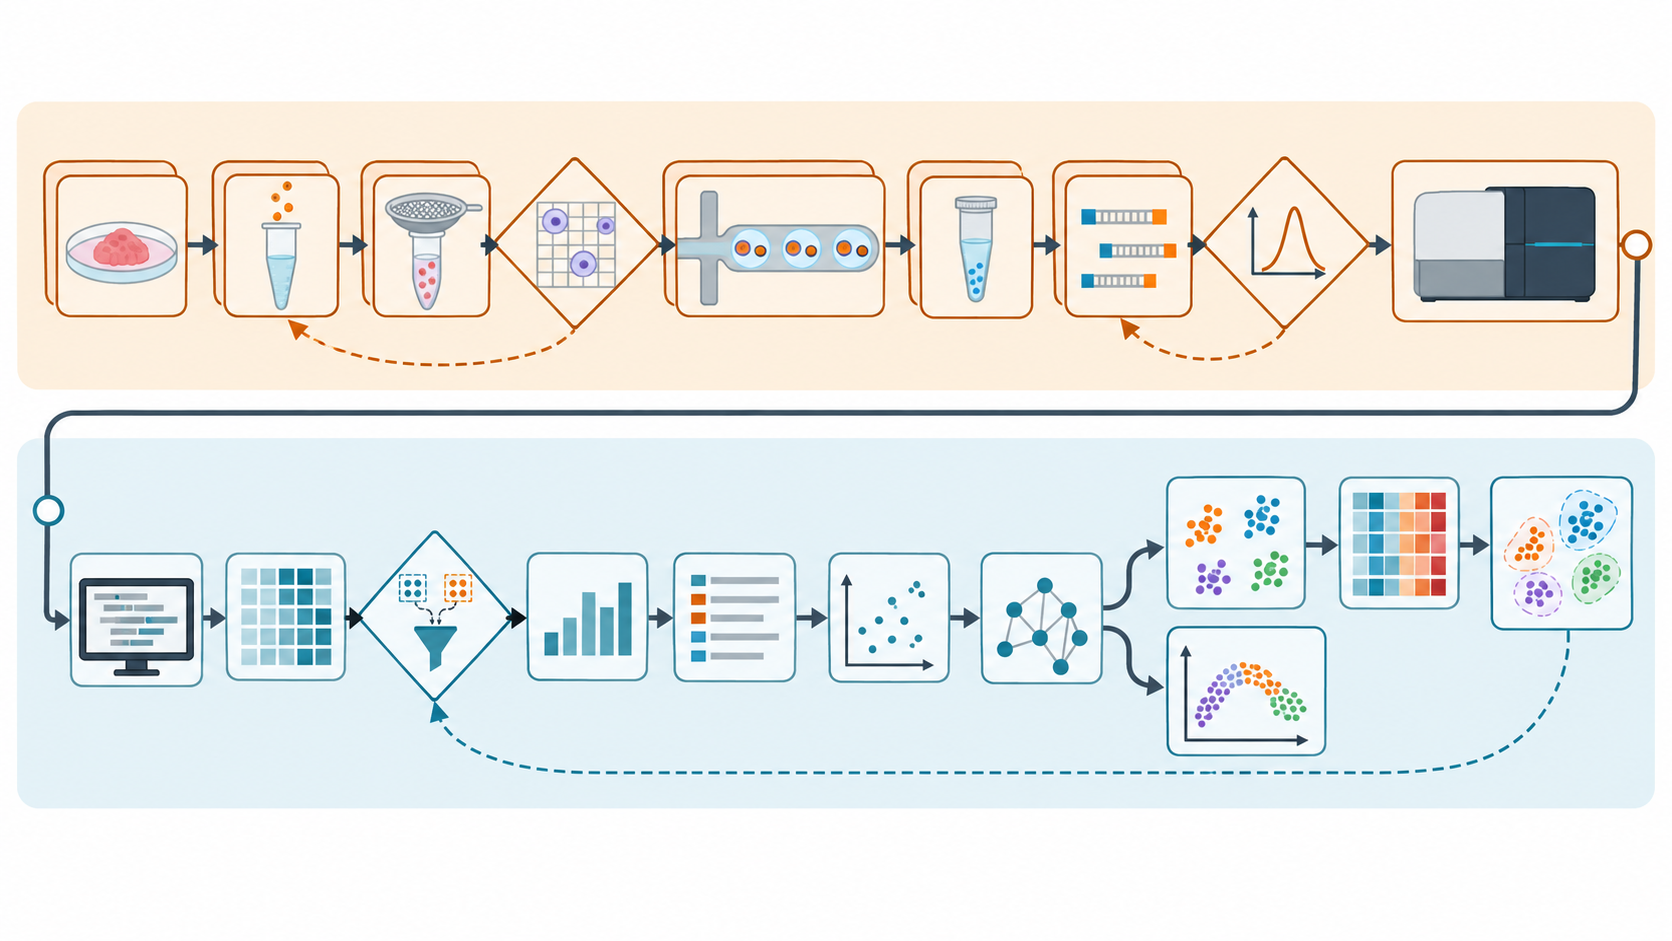
\includegraphics[width=\linewidth]{figures/ch06/ch06-05-v2-brief.png}};
\begin{scope}[x={(img.south east)},y={(img.north west)}]
  \tikzset{
    okmark/.style={draw=white,line width=0.6pt,fill=ChSixGood,text=white,circle,font=\sffamily\bfseries\tiny,inner sep=0.6pt,minimum size=3.6mm},
    ngmark/.style={draw=white,line width=0.6pt,fill=ChSixBad,text=white,circle,font=\sffamily\bfseries\tiny,inner sep=0.6pt,minimum size=3.6mm}
  }
  \node[okmark] at (0.07,0.85) {$\checkmark$};
  \node[okmark] at (0.16,0.85) {$\checkmark$};
  \node[okmark] at (0.25,0.85) {$\checkmark$};
  \node[ngmark] at (0.34,0.86) {$\times$};
  \node[okmark] at (0.25,0.60) {$\checkmark$};
  \node[okmark] at (0.46,0.85) {$\checkmark$};
  \node[okmark] at (0.58,0.85) {$\checkmark$};
  \node[okmark] at (0.67,0.85) {$\checkmark$};
  \node[ngmark] at (0.77,0.86) {$\times$};
  \node[okmark] at (0.72,0.61) {$\checkmark$};
  \node[ngmark] at (0.83,0.77) {$\times$};
  \node[ngmark] at (0.98,0.79) {$\times$};
  \node[okmark] at (0.08,0.44) {$\checkmark$};
  \node[okmark] at (0.17,0.44) {$\checkmark$};
  \node[ngmark] at (0.26,0.47) {$\times$};
  \node[ngmark] at (0.35,0.44) {$\times$};
  \node[okmark] at (0.44,0.44) {$\checkmark$};
  \node[okmark] at (0.53,0.44) {$\checkmark$};
  \node[okmark] at (0.62,0.44) {$\checkmark$};
  \node[okmark] at (0.68,0.42) {$\checkmark$};
  \node[okmark] at (0.68,0.25) {$\checkmark$};
  \node[okmark] at (0.84,0.52) {$\checkmark$};
  \node[ngmark] at (0.93,0.52) {$\times$};
  \node[okmark] at (0.58,0.14) {$\checkmark$};
\end{scope}
\end{tikzpicture}
\caption{按完整任务书整图生成的流程图底图（无文字）及逐项核对。绿色“$\checkmark$”为与步骤表一致的节点或箭头，红色“$\times$”为错误或缺失。本次生成虽然画对了近邻图分叉与三条指定反馈弧，但在质控菱形双样本叠卡、两处样本合并点、跨泳道连接箭头、可选小框位置及终点空白标签牌等 7 处位置仍存在结构偏差；因此终稿改为由作者绘制结构，模型只生成图标。}\label{fig:ch06-05}
\end{figure}

打印步骤表在图~\ref{fig:ch06-05} 上逐个节点、逐条箭头打勾核验，如实记录观察结果：本次生成确实做到了全图无文字，20 个主步骤图标的先后顺序、下排第 7 格近邻图向聚类与二维嵌入的分叉，以及三条指定虚线反馈弧（Q1 $\rightarrow$ W2、Q2 $\rightarrow$ W6、C11 $\rightarrow$ Q3）全部正确；但图上标出的 7 处红叉（$\times$）暴露出整图生成难以克服的结构短板：
\begin{enumerate}
\item \textbf{双样本叠卡不完整（上排第 4、第 8 格“$\times$”）：}提示词要求湿实验第 1 至 8 步每一步都画成双层叠放卡片，但模型只在 6 个圆角矩形步骤画了叠卡，两处菱形质控（Q1、Q2）却只画了单层菱形。
\item \textbf{两处样本合并点缺失（上排测序仪前与下排第 4 格“$\times$”）：}文库质控到测序仪之间只有单根箭头，没有画出两条样本文库线汇合入测序仪；下排第 4 格标准化柱状图处同样看不出两个样本的过滤后矩阵在此合并。
\item \textbf{跨泳道连接箭头不清（上排最右端“$\times$”）：}右上角连接圆圈直接贴在测序仪边框上，缺少从测序仪指向圆圈的独立交接箭头，也未留出放置产物 FASTQ 的位置。
\item \textbf{可选步骤位置错位（下排第 3 格“$\times$”）：}提示词要求把两个虚线可选小框（C3a、C3b）画在细胞质控菱形上方再汇入，模型却把两个带小点的虚线小方框直接塞进了菱形内部，无法叠加文字标签。
\item \textbf{终点与图标细节偏差（下排最右端“$\times$”）：}注释终点只画了包绕点簇的虚线轮廓，漏掉了提示词要求的空白圆角标签牌；上排第 6 步的 PCR 管画得偏长、像普通离心管，且部分器皿仍带渐变与立体透视。
\end{enumerate}

V2 实验证明：整图生成能提供色彩与风格方向，但逐项核对和返工的成本远高于直接画骨架，而且每次重生成都必须把全部二十多个节点和箭头从头复查一遍。

因此，更可靠的分工是改用\textbf{“图标表模式”（V3）}：不再让图像模型画箭头和泳道，而是在一张 $4 \times 3$ 网格的白底画布上，一次生成 12 个风格统一、彼此独立的步骤图标，切分后嵌入图~\ref{fig:ch06-03} 的确定性骨架。在 \scidraw{} 中，作者可从流程图入口（\sdtool{workflow-diagram-generator}）或科研绘图向导（\sdtool{figure-workflow}）“机制与流程图”路线进入绘图工作台（\sdtool{ai-drawing}），用提示词模式生成如下 12 宫格图标表：

\begin{Prompt}
A sheet of twelve flat vector scientific icons arranged in an even grid of four columns
and three rows on a pure white background. Each icon sits centred in its own invisible
square cell with wide white margins and does not touch any other icon. Uniform dark slate
outline of medium weight, flat fills, no gradients, no shadows, no 3D.
Row 1 (warm muted orange-brown accent #B5653A with pale beige fills):
 1. small piece of pink soft tissue on a shallow petri dish;
 2. conical centrifuge tube with three tiny droplets falling into it;
 3. round cell strainer mesh sitting on top of a tube;
 4. square counting grid with five round cells, one cell drawn darker.
Row 2 (same warm accent, except icon 8 in deep amber #8A6D1F):
 5. rectangular microfluidic chip with one channel pinching off round droplets,
    each droplet containing one small cell and one small bead;
 6. single small PCR tube with a closed cap;
 7. three short double-stranded DNA fragments, each with small coloured end caps;
 8. benchtop sequencing instrument: a box with a small slot holding a flow cell.
Row 3 (muted teal-blue accent #2F6F8F with pale blue-grey fills):
 9. computer monitor showing short horizontal bars aligned under one long bar;
10. square grid matrix of small cells with varied light-to-dark shading;
11. network of dots connected by thin edges;
12. four clusters of dots in different muted colours, with blank rounded tag shapes.
No text, no letters, no numbers, no labels, no arrows, no microscope, no DNA helix. 4:3.
\end{Prompt}

拿到 $4 \times 3$ 图标整表后，必须对 12 个图标逐格做科学核验：（1）浅培养皿上是粉红软组织小块，而非完整器官；（2）锥底离心管上方恰好落下 3 滴酶液，管上只有无字刻度线；（3）圆形筛网架在管口上；（4）计数方格内恰好 5 个圆细胞、1 个着色更深，无非圆杂物或文字；（5）微流控芯片单通道缩颈后方 3 个微滴，每滴含一较大细胞与一较小深色凝胶珠；（6）带扣盖的单个小 PCR 管；（7）3 段双链梯状短片段配彩色端帽，不是长链双螺旋装饰；（9）显示器内一条长横条下对齐多条短横条；（10）深浅变化的方格计数矩阵；（11）点与细边组成的近邻网络，无化学元素符号；（12）4 个不同色相的点簇，每簇旁各有一个空白圆角标签框。放大至 200\% 检查，全表无任何字母或数字残留。

唯独第 8 格（桌面测序仪）初稿不合格：机箱前方伸出了一个斜托盘，上面摆着条纹薄片，远看像一台办公打印机。由于图标表各格独立，我们无需重画全表，只需在 \scidraw{} 绘图历史中选中该测序仪图标作为参考图继续修改，下达只替换前方托盘为封闭式光学流动池卡匣的修改指令：

\begin{Prompt}
Edit only this one sequencing-instrument icon. Preserve its simple scientific icon style,
dark slate outline, white background, and square framing. Replace the printer-like front
paper tray and paper-output slot with a small closed optical flow-cell cartridge bay:
a glass rectangular microfluidic flow cell in a shallow enclosed cartridge, with tiny
parallel fluidic channels visible through a small window. Use flat pale beige fills with
a restrained deep amber #8A6D1F accent on the cartridge. No sheets of paper, no paper
trays, no keyboards, no text, no letters, no numbers, no labels, no logos. Aspect 1:1.
\end{Prompt}

单图标修改后，像打印机的外伸纸托消失，前面板中央换成了深琥珀色边框的玻璃微流控流动池窗口，内部可见平行折返流道。将图标表按 $4 \times 3$ 等分网格裁切、将近白背景转为透明通道并保留约 6\% 留白边距，即可放入骨架图。

\section{贯穿案例：单细胞 RNA 测序流程从初稿到终稿}

现在我们将小陈从 V1 初稿一路推进到 V4 终稿的完整过程串联起来：

\textbf{第一步：从 V1 初稿退回写步骤表与任务书。}
面对一句话提示词生成的 V1 初稿（图~\ref{fig:ch06-01}），小陈不再在提示词框里盲目打补丁，而是退回方法记录整理出表~\ref{tab:ch06-01} 的步骤表，并完成表~\ref{tab:ch06-02} 的九项实验条件核实。接着，她在 \scidraw{} 科研绘图向导（\sdtool{figure-workflow}）选择“机制与流程图”路线，替换默认任务书并下载本地副本：

\begin{Prompt}
【目的】让读者看清：从小鼠肺组织到细胞类型注释，每一步做什么、交给下一步什么；
         哪些是湿实验、哪些是计算；两个样本在哪里并行、在哪里合并；质控不通过时回到哪里。
【读者与用途】论文 Figure 1A 方法流程图；读者为熟悉分子生物学的同行。
         终稿可按双栏通栏 174 mm 宽缩排。
【必须出现的对象】步骤表 6-1 的全部主节点（W1–W6、Q1、Q2、S1、C1–C11）与可选节点
         （W3a、W3b、C3a、C3b、C6a），以及 6 类核心交接产物：单细胞悬液、带条形码的 cDNA、
         测序文库、FASTQ、过滤后计数矩阵、注释后的细胞图谱（另含原始矩阵与 UMAP 坐标）。
【关系与箭头含义】实线箭头 = 顺序与交接；虚线弧 = 反馈/返回；菱形 = 质控，两个出口；
         虚线框 = 可选步骤；圆形连接符 A = 跨行续接；流程箭头不表示因果。
【已知、假设与待确认】步骤顺序为通用流程，已确认；所有参数为〔作者填写〕，图中不写参数；
         整合/批次校正的位置为简化，图注说明。
【不可改变的科学信息】聚类与 UMAP 都从近邻图分出，UMAP 不连向聚类或注释；
         两个样本的文库在测序前混合，计数矩阵在标准化前合并。
【构图与标签】两条水平泳道：上为湿实验（含测序），下为计算分析，均从左到右阅读；
         上下由连接符 A（FASTQ）衔接。标签为中文，分子与软件名保留英文。
         湿实验暖色、计算冷色；每个泳道一种强调色。
【参考材料】步骤表 6-1；方法记录；Luecken & Theis 2019；Zheng et al. 2017。
【自查标准】节点数、箭头数、分支与合并点与步骤表逐一对应；没有未列出的步骤或装饰；
         图中无参数数值；在最终尺寸下 7 pt 文字可读。
\end{Prompt}

\textbf{第二步：用确定性骨架合并 AI 图标，合成 V4 终稿。}
在对比了确定性骨架（图~\ref{fig:ch06-03}）与 V2 整图生成（图~\ref{fig:ch06-05}）之后，小陈保持图~\ref{fig:ch06-03} 的全部节点坐标、箭头、分叉、反馈弧与文字标签一概不动，仅在 12 个主要步骤框正上方各放置一枚切分核验后的透明背景图标（01 $\rightarrow$ W1 组织采集；02 $\rightarrow$ W2 组织解离；03 $\rightarrow$ W3 过滤与清洗；04 $\rightarrow$ Q1 计数与活率；05 $\rightarrow$ W4 微滴捕获；06 $\rightarrow$ W5 逆转录与扩增；07 $\rightarrow$ W6 文库构建；08 $\rightarrow$ S1 混合与测序；09 $\rightarrow$ C1 比对与计数；10 $\rightarrow$ C2 细胞识别；11 $\rightarrow$ C7 $k$ 近邻图；12 $\rightarrow$ C11 细胞类型注释），其余节点保持纯文字框，避免过度装饰。合成后的终稿见图~\ref{fig:ch06-06}。

\begin{figure}[htbp]\centering
\resizebox{\linewidth}{!}{% FIG ch06-06 final (Chinese) — same structure as skeleton + icons%
\def\ChSixShowIcons{}%
% Shared styles for chapter 6 workflow TikZ figures.%
% Every figure inputs this file, so commands are defined with \providecommand.%
\providecolor{BookTeal}{HTML}{176C68}%
\providecolor{BookInk}{HTML}{23363E}%
\providecolor{BookRule}{HTML}{C8D6D6}%
\providecolor{BookPale}{HTML}{F1F6F5}%
\definecolor{WetPale}{HTML}{FBF1EA}%
\definecolor{Wet}{HTML}{B5653A}%
\definecolor{Seq}{HTML}{8A6D1F}%
\definecolor{DryPale}{HTML}{EEF4F7}%
\definecolor{Dry}{HTML}{2F6F8F}%
\definecolor{ChSixFeedback}{HTML}{7A8A90}%
\definecolor{ChSixBad}{HTML}{C0392B}%
\usetikzlibrary{arrows.meta,positioning,shapes.geometric,shapes.misc,fit,backgrounds,calc}%
\ifdefined\ChSixLayersReady\else%
  \pgfdeclarelayer{chsixlane}%
  \pgfsetlayers{chsixlane,background,main}%
  \def\ChSixLayersReady{}%
\fi%

\tikzset{%
  chsix/.style={font=\sffamily\scriptsize, text=BookInk, align=center},%
  flowstep/.style={%
    chsix, rounded corners=2pt, draw=Wet, line width=0.45pt, fill=white,%
    text width=19mm, minimum height=7.4mm, inner sep=1.3pt,%
  },%
  flowstepdry/.style={flowstep, draw=Dry},%
  flowstepseq/.style={flowstep, draw=Seq},%
  artifact/.style={%
    chsix, trapezium, trapezium left angle=70, trapezium right angle=110,%
    trapezium stretches=true,%
    draw=BookInk, line width=0.45pt, fill=white,%
    minimum height=6.2mm, inner sep=1.2pt,%
  },%
  gate/.style={%
    chsix, diamond, aspect=1.7, draw=BookInk, line width=0.45pt, fill=white,%
    text width=12mm, inner sep=0.6pt, minimum height=8mm,%
  },%
  opt/.style={flowstep, dashed, draw=BookInk!70},%
  optdry/.style={flowstepdry, dashed, draw=BookInk!70},%
  stack/.style={flowstep},%
  link/.style={-{Stealth[length=1.6mm]}, semithick, draw=BookInk},%
  linkthin/.style={-{Stealth[length=1.2mm]}, thin, draw=BookInk!80},%
  back/.style={-{Stealth[length=1.5mm]}, dashed, draw=ChSixFeedback},%
  conn/.style={%
    circle, draw=BookInk, line width=0.5pt, minimum size=4.6mm,%
    font=\sffamily\scriptsize\bfseries, inner sep=0pt, text=BookInk,%
  },%
  lanetitle/.style={font=\sffamily\bfseries\small, text=BookInk, align=left},%
  passlabel/.style={font=\sffamily\scriptsize, text=BookInk, fill=white, inner sep=0.7pt, align=center},%
  mergelabel/.style={font=\sffamily\scriptsize, text=BookInk, fill=white, inner sep=0.8pt, align=center},%
  taglab/.style={font=\sffamily\scriptsize, text=ChSixFeedback, fill=white, inner sep=0.8pt, align=center},%
  gramcap/.style={font=\sffamily\scriptsize, text=BookInk, align=left, anchor=west},%
}%

% Offset card behind a two-sample step. Text stays on the front node only.%
\providecommand{\ChSixCardBack}[1]{%
  \begin{pgfonlayer}{background}%
    \draw[Wet, line width=0.45pt, rounded corners=2pt, fill=white]%
      ([shift={(-0.55mm,0.55mm)}]#1.south west)%
      rectangle ([shift={(-0.55mm,0.55mm)}]#1.north east);%
  \end{pgfonlayer}%
}%
% #1 options, #2 name, #3 position (with parentheses), #4 text%
\providecommand{\ChSixCard}[4]{%
  \node[stack, #1] (#2) at #3 {#4};%
  \ChSixCardBack{#2}%
}%

\providecommand{\ChSixMaybeLabel}[1]{%
  \ifdefined\nolabels\else#1\fi%
}%

\providecommand{\ChSixIcon}[2]{%
  \ifdefined\ChSixShowIcons%
    \IfFileExists{#1}{%
      \node[anchor=south, inner sep=0] at ([yshift=0.7mm]#2.north)%
        {\includegraphics[height=5.4mm]{#1}};%
    }{}%
  \fi%
}%
%
% Chinese node labels for FIG ch06-03 / ch06-06%
\providecommand{\ChSixLaneWet}{湿实验与测序}%
\providecommand{\ChSixLaneDry}{计算分析}%
\providecommand{\ChSixTxtWone}{组织采集}%
\providecommand{\ChSixTxtWtwo}{组织解离}%
\providecommand{\ChSixTxtWthree}{过滤与清洗}%
\providecommand{\ChSixTxtWthreeA}{红细胞裂解}%
\providecommand{\ChSixTxtWthreeB}{死细胞去除}%
\providecommand{\ChSixTxtQone}{计数与\\活率}%
\providecommand{\ChSixTxtWfour}{微滴捕获与\\条形码标记}%
\providecommand{\ChSixTxtWfive}{逆转录与\\cDNA 扩增}%
\providecommand{\ChSixTxtWsix}{文库构建}%
\providecommand{\ChSixTxtQtwo}{文库\\质控}%
\providecommand{\ChSixTxtSone}{文库混合\\与测序}%
\providecommand{\ChSixTxtCone}{比对与\\UMI 计数}%
\providecommand{\ChSixTxtCtwo}{细胞识别}%
\providecommand{\ChSixTxtQthree}{细胞\\质控}%
\providecommand{\ChSixTxtCthreeA}{双细胞检测}%
\providecommand{\ChSixTxtCthreeB}{环境 RNA\\校正}%
\providecommand{\ChSixTxtCfour}{合并与\\标准化}%
\providecommand{\ChSixTxtCfive}{高变基因}%
\providecommand{\ChSixTxtCsix}{PCA 降维}%
\providecommand{\ChSixTxtCsixA}{整合（可选）}%
\providecommand{\ChSixTxtCseven}{k 近邻图}%
\providecommand{\ChSixTxtCeight}{聚类\\（Leiden）}%
\providecommand{\ChSixTxtCnine}{UMAP}%
\providecommand{\ChSixTxtCten}{标志基因}%
\providecommand{\ChSixTxtCeleven}{细胞类型\\注释}%
\providecommand{\ChSixArtSusp}{单细胞悬液}%
\providecommand{\ChSixArtCdna}{带条形码\\的 cDNA}%
\providecommand{\ChSixArtLib}{测序文库}%
\providecommand{\ChSixArtFastq}{FASTQ}%
\providecommand{\ChSixArtRaw}{原始计数\\矩阵}%
\providecommand{\ChSixArtFilt}{过滤后矩阵}%
\providecommand{\ChSixArtAtlas}{注释后的\\细胞图谱}%
\providecommand{\ChSixArtUmap}{UMAP 坐标\\（仅用于展示）}%
\providecommand{\ChSixQoneFail}{不合格：\\优化解离}%
\providecommand{\ChSixQtwoFail}{不合格}%
\providecommand{\ChSixCelevenFail}{发现低质量簇\\或分辨率不当}%
\providecommand{\ChSixMergeNote}{两样本在此合并}%
\providecommand{\ChSixPass}{通过}%
%
\begin{tikzpicture}[x=1cm,y=1cm]%
  % Row positions are set with relative anchors in ch06-workflow-draw.tex%
% so Chinese and English labels do not share one set of fixed centres.%
%
  % Workflow structure (FIG ch06-03 skeleton / ch06-06 final).%
% Requires ch06-styles and a label file. Nodes are placed from the node%
% above them so wrapped English labels cannot land on the next row.%
\coordinate (origin) at (0,0);%
% Final figures carry icons above the nodes; keep feedback arcs above them.%
\ifdefined\ChSixShowIcons
  \def\ChSixLift{6.6mm}%
  \def\ChSixArc{12.2mm}%
\else
  \def\ChSixLift{0mm}%
  \def\ChSixArc{8.4mm}%
\fi

% ----- Wet lab, row 1: collection through droplet capture -----%
\ChSixCard{anchor=north west}{nW1}{(origin)}{\ChSixMaybeLabel{\ChSixTxtWone}}%
\ChSixCard{anchor=west}{nW2}{([xshift=3.2mm]nW1.east)}{\ChSixMaybeLabel{\ChSixTxtWtwo}}%
\ChSixCard{anchor=west}{nW3}{([xshift=3.2mm]nW2.east)}{\ChSixMaybeLabel{\ChSixTxtWthree}}%
\node[gate, anchor=west] (nQ1) at ([xshift=3.6mm]nW3.east) {\ChSixMaybeLabel{\ChSixTxtQone}};%
\ChSixCard{anchor=west}{nW4}{([xshift=6.4mm]nQ1.east)}{\ChSixMaybeLabel{\ChSixTxtWfour}}%

\draw[link] (nW1) -- (nW2);%
\draw[link] (nW2) -- (nW3);%
\draw[link] (nW3) -- (nQ1);%
\draw[link] (nQ1) -- (nW4);%

\coordinate (arcQ1) at ($(nW2.north)!0.5!(nQ1.north)+(0,\ChSixArc)$);%
\draw[back] ([yshift=\ChSixLift]nQ1.north) -- ([yshift=\ChSixLift]nQ1.north |- arcQ1) -- ([yshift=\ChSixLift]nW2.north |- arcQ1) -- ([yshift=\ChSixLift]nW2.north);%
\node[taglab, anchor=south] (q1fail) at (arcQ1) {\ChSixMaybeLabel{\ChSixQoneFail}};%
\node[passlabel] (passQ1) at ($(nQ1.east)!0.5!(nW4.west)+(0,1.3mm)$) {\ChSixMaybeLabel{\ChSixPass}};%

\node[lanetitle, anchor=south west] (laneWet) at ([yshift=1.2mm]q1fail.north -| origin) {\ChSixMaybeLabel{\ChSixLaneWet}};%

% Optional lysis / dead-cell removal under filtering, product to their right.%
\node[opt, anchor=north] (nW3a) at ([yshift=-2.2mm]nW3.south) {\ChSixMaybeLabel{\ChSixTxtWthreeA}};%
\node[opt, anchor=north] (nW3b) at ([yshift=-1.8mm]nW3a.south) {\ChSixMaybeLabel{\ChSixTxtWthreeB}};%
\draw[linkthin] (nW3.south) -- (nW3a.north);%
\draw[linkthin] (nW3a.south) -- (nW3b.north);%
\node[artifact, anchor=north west] (aSusp) at ([xshift=3.2mm, yshift=-2.2mm]nW3.south east) {\ChSixMaybeLabel{\ChSixArtSusp}};%

% ----- Wet lab, row 2 (left-aligned; FASTQ is the hand-off into connector A) -----%
\ChSixCard{anchor=north west}{nW5}{([yshift=-10mm]nW3b.south -| nW1.west)}{\ChSixMaybeLabel{\ChSixTxtWfive}}%
\ChSixCard{anchor=west}{nW6}{([xshift=2.4mm]nW5.east)}{\ChSixMaybeLabel{\ChSixTxtWsix}}%
\node[gate, anchor=west] (nQ2) at ([xshift=2.4mm]nW6.east) {\ChSixMaybeLabel{\ChSixTxtQtwo}};%
\node[flowstepseq, anchor=west] (nS1) at ([xshift=6.2mm]nQ2.east) {\ChSixMaybeLabel{\ChSixTxtSone}};%
\node[artifact, anchor=west] (aFastq) at ([xshift=2.2mm]nS1.east) {\ChSixMaybeLabel{\ChSixArtFastq}};%
\node[conn, anchor=west] (nA) at ([xshift=2mm]aFastq.east) {A};%

\draw[link] (nW5) -- (nW6);%
\draw[link] (nW6) -- (nQ2);%
\draw[link] (nQ2) -- (nS1);%
\draw[link] (nS1) -- (aFastq);%
\draw[link] (aFastq) -- (nA);%
\node[passlabel] (passQ2) at ($(nQ2.east)!0.5!(nS1.west)+(0,1.3mm)$) {\ChSixMaybeLabel{\ChSixPass}};%

\coordinate (arcQ2) at ($(nW6.north)!0.5!(nQ2.north)+(0,\ChSixArc)$);%
\draw[back] ([yshift=\ChSixLift]nQ2.north) -- ([yshift=\ChSixLift]nQ2.north |- arcQ2) -- ([yshift=\ChSixLift]nW6.north |- arcQ2) -- ([yshift=\ChSixLift]nW6.north);%
\node[taglab, anchor=south] (q2fail) at (arcQ2) {\ChSixMaybeLabel{\ChSixQtwoFail}};%

\node[artifact, anchor=north] (aCdna) at ([yshift=-2mm]$(nW5.south)!0.5!(nW6.south)$) {\ChSixMaybeLabel{\ChSixArtCdna}};%
\node[artifact, anchor=north] (aLib) at ([yshift=-2mm]$(nW6.south)!0.5!(nQ2.south)$) {\ChSixMaybeLabel{\ChSixArtLib}};%

% ----- Computational lane -----%
\node[conn, anchor=north west] (nA2) at ([yshift=-7mm]aCdna.south -| origin) {A};%
\node[flowstepdry, anchor=west] (nC1) at ([xshift=3.2mm]nA2.east) {\ChSixMaybeLabel{\ChSixTxtCone}};%
\node[flowstepdry, anchor=west] (nC2) at ([xshift=3.6mm]nC1.east) {\ChSixMaybeLabel{\ChSixTxtCtwo}};%
\node[gate, anchor=west] (nQ3) at ([xshift=4.2mm]nC2.east) {\ChSixMaybeLabel{\ChSixTxtQthree}};%
\node[flowstepdry, anchor=west] (nC4) at ([xshift=4.2mm]nQ3.east) {\ChSixMaybeLabel{\ChSixTxtCfour}};%
\node[flowstepdry, anchor=west] (nC5) at ([xshift=3.6mm]nC4.east) {\ChSixMaybeLabel{\ChSixTxtCfive}};%

\draw[link] (nA2) -- (nC1);%
\draw[link] (nC1) -- (nC2);%
\draw[link] (nC2) -- (nQ3);%
\draw[link] (nQ3) -- (nC4);%
\draw[link] (nC4) -- (nC5);%

\node[mergelabel, anchor=south] (mergeNote) at ([yshift=1mm]nC4.north) {\ChSixMaybeLabel{\ChSixMergeNote}};%

\coordinate (arcDry) at ($(nC1.north)!0.5!(nQ3.north)+(0,\ChSixArc)$);%
\node[taglab, anchor=south, text width=28mm] (c11fail) at (arcDry) {\ChSixMaybeLabel{\ChSixCelevenFail}};%
\node[lanetitle, anchor=south west] (laneDry) at ([yshift=1.2mm]c11fail.north -| origin) {\ChSixMaybeLabel{\ChSixLaneDry}};%

% Optional doublet / ambient RNA under the cell-QC gate.%
\node[optdry, anchor=north east] (nC3a) at ([yshift=-2mm, xshift=-1mm]nQ3.south) {\ChSixMaybeLabel{\ChSixTxtCthreeA}};%
\node[optdry, anchor=north west] (nC3b) at ([yshift=-2mm, xshift=1mm]nQ3.south) {\ChSixMaybeLabel{\ChSixTxtCthreeB}};%
\draw[linkthin] (nQ3.south) -- (nC3a.north);%
\draw[linkthin] (nQ3.south) -- (nC3b.north);%
\draw[linkthin] (nC3a.south) -- ++(0,-2.4mm) -| (nC3b.south);%

\node[artifact, anchor=north] (aRaw) at ([yshift=-2mm]$(nC1.south)!0.5!(nC2.south)$) {\ChSixMaybeLabel{\ChSixArtRaw}};%
\node[artifact, anchor=north] (aFilt) at ([yshift=-2mm]nC4.south) {\ChSixMaybeLabel{\ChSixArtFilt}};%

% Fork: k-NN graph splits to clustering (continues) and UMAP (display only).%
\node[flowstepdry, anchor=north west] (nC6) at ([yshift=-4mm]aRaw.south -| nC1.west) {\ChSixMaybeLabel{\ChSixTxtCsix}};%
\node[flowstepdry, anchor=west] (nC7) at ([xshift=4mm]nC6.east) {\ChSixMaybeLabel{\ChSixTxtCseven}};%
\node[flowstepdry, anchor=west] (nC8) at ([xshift=5mm]nC7.east) {\ChSixMaybeLabel{\ChSixTxtCeight}};%
\node[flowstepdry, anchor=west] (nC10) at ([xshift=3.6mm]nC8.east) {\ChSixMaybeLabel{\ChSixTxtCten}};%
\node[flowstepdry, anchor=west] (nC11) at ([xshift=3.6mm]nC10.east) {\ChSixMaybeLabel{\ChSixTxtCeleven}};%
\node[optdry, anchor=north] (nC6a) at ([yshift=-2mm]nC6.south) {\ChSixMaybeLabel{\ChSixTxtCsixA}};%
\node[flowstepdry, anchor=north] (nC9) at ([yshift=-3.2mm]nC7.south) {\ChSixMaybeLabel{\ChSixTxtCnine}};%
\node[artifact, anchor=north, text width=22mm] (aUmap) at ([yshift=-1.8mm]nC9.south) {\ChSixMaybeLabel{\ChSixArtUmap}};%
\node[artifact, anchor=north] (aAtlas) at ([yshift=-2mm]$(nC10.south)!0.5!(nC11.south)$) {\ChSixMaybeLabel{\ChSixArtAtlas}};%

\draw[link] (nC5.south) -- ++(0,-2.5mm) -| (nC6.north);%
\draw[linkthin] (nC6.south) -- (nC6a.north);%
\draw[link] (nC6) -- (nC7);%
\draw[link] (nC7) -- (nC8);%
\draw[link] (nC8) -- (nC10);%
\draw[link] (nC10) -- (nC11);%
\draw[link] (nC7.south) -- (nC9.north);%

% Return from annotation to clustering, and the long return to cell QC.%
\coordinate (bus) at ([yshift=-4.5mm]aUmap.south);%
\draw[back] (nC11.south) -- (nC11.south |- bus) -- (nC8.south |- bus) -- (nC8.south);%
\draw[back] (nC11.east) -- ++(3.2mm,0) |- (c11fail.east);%
\draw[back] (c11fail.west) -| ([yshift=\ChSixLift]nQ3.north);%

% Connector A joins the lanes in the gutter between them.%
\draw[link] (nA.south) -- ++(0,-2.2mm) -| (nA2.north);%

\ChSixIcon{figures/ch06/icons/ch06-icon-01.png}{nW1}%
\ChSixIcon{figures/ch06/icons/ch06-icon-02.png}{nW2}%
\ChSixIcon{figures/ch06/icons/ch06-icon-03.png}{nW3}%
\ChSixIcon{figures/ch06/icons/ch06-icon-04.png}{nQ1}%
\ChSixIcon{figures/ch06/icons/ch06-icon-05.png}{nW4}%
\ChSixIcon{figures/ch06/icons/ch06-icon-06.png}{nW5}%
\ChSixIcon{figures/ch06/icons/ch06-icon-07.png}{nW6}%
\ChSixIcon{figures/ch06/icons/ch06-icon-08.png}{nS1}%
\ChSixIcon{figures/ch06/icons/ch06-icon-09.png}{nC1}%
\ChSixIcon{figures/ch06/icons/ch06-icon-10.png}{nC2}%
\ChSixIcon{figures/ch06/icons/ch06-icon-11.png}{nC7}%
\ChSixIcon{figures/ch06/icons/ch06-icon-12.png}{nC11}%

\begin{pgfonlayer}{chsixlane}%
  \node[rectangle, fit=(laneWet)(nW1)(nW4)(nW3b)(aSusp)(nA)(aCdna)(aLib)(q1fail),%
        fill=WetPale, draw=none, inner sep=1.1mm] {};%
  \node[rectangle, fit=(laneDry)(nA2)(nC5)(nC11)(nC6a)(aUmap)(aAtlas)(c11fail)(nC3a)(nC3b),%
        fill=DryPale, draw=none, inner sep=1.1mm] {};%
\end{pgfonlayer}%
%
\end{tikzpicture}%
}
\caption{液滴法单细胞 RNA 测序的实验与分析流程（示意）。上：湿实验与测序（暖色泳道）。对照与处理样本分别完成解离、捕获与文库构建（叠放的框），文库混合后测序。下：计算分析（冷色泳道），经连接符 A 由 FASTQ 衔接。菱形为质控，虚线弧表示不通过或结果异常时返回；虚线框为可选步骤。聚类与 UMAP 都基于主成分空间的 $k$ 近邻图，UMAP 仅用于展示。本图为通用流程的简化，未画出具体参数、细胞核测序、样本条形码复用、轨迹与差异丰度分析；整合/批次校正的位置因软件而异。图标由图像生成模型制作并经人工核对，流程结构与文字由作者绘制。}\label{fig:ch06-06}
\end{figure}

\textbf{第三步：编写双语图注并逐项填写终稿核验表。}
在 \scidraw{} 图注辅助（\sdtool{figure-legend}）起草的描述基础上，小陈补齐了简化范围、算法位置差异及 AI 分工声明，定稿中英文图注如下：

\begin{BookNote}
\textbf{图 6-6　液滴法单细胞 RNA 测序的实验与分析流程（示意）。} 上：湿实验与测序（暖色泳道）。对照与处理样本分别完成解离、捕获与文库构建（叠放的框），文库混合后测序。下：计算分析（冷色泳道），经连接符 A 由 FASTQ 衔接。菱形为质控，虚线弧表示不通过或结果异常时返回；虚线框为可选步骤。聚类与 UMAP 都基于主成分空间的 $k$ 近邻图，UMAP 仅用于展示。本图为通用流程的简化，未画出具体参数、细胞核测序、样本条形码复用、轨迹与差异丰度分析；整合/批次校正的位置因软件而异。图标由图像生成模型制作并经人工核对，流程结构与文字由作者绘制。

\medskip
\textbf{Figure 6-6 | Experimental and computational workflow for droplet-based single-cell RNA sequencing (schematic).} Top, wet-lab and sequencing steps (warm lane): control and treated samples are dissociated, captured and converted to libraries separately (stacked boxes) and pooled for sequencing. Bottom, computational analysis (cool lane), continued from FASTQ files via connector A. Diamonds are quality-control gates; dashed arcs return to an earlier step when a gate fails or results are anomalous; dashed boxes are optional steps. Clustering and UMAP are both computed from the $k$-nearest-neighbour graph in principal-component space; UMAP is used for display only. The diagram simplifies a generic protocol and omits parameters, single-nucleus protocols, sample multiplexing, trajectory and differential-abundance analyses; where integration sits varies between software packages. Icons were made with an image-generation model and checked by hand; the workflow structure and all text were drawn by the authors.
\end{BookNote}

交付前，小陈先用图片检查（\sdtool{figure-checker}）检查版面尺寸、灰度对比度与色觉可辨性，再对照表~\ref{tab:ch06-01} 逐行完成终稿核验记录（表~\ref{tab:ch06-04}）。

\begin{table}[htbp]\centering\footnotesize
\setlength{\tabcolsep}{4pt}
\renewcommand{\arraystretch}{1.15}
\caption{单细胞 RNA 测序流程图终稿（图~\ref{fig:ch06-06}）逐项核验记录。}\label{tab:ch06-04}
\begin{tabularx}{\linewidth}{@{}>{\raggedright\arraybackslash}p{22mm}YY@{}}
\toprule
\textbf{检查项} & \textbf{任务书与步骤表期望} & \textbf{图~\ref{fig:ch06-06} 终稿核验结果} \\
\midrule
节点数 & 主节点 20 个（湿实验与测序 W1–W6、Q1、Q2、S1 共 9 个；计算 C1–C11、Q3 共 11 个）+ 可选节点 5 个（W3a、W3b、C3a、C3b、C6a）+ 产物 8 个 & 全部在位，与图~\ref{fig:ch06-03} 骨架完全同构 \\
顺序箭头 & 每条实线箭头与表~\ref{tab:ch06-01}“下游”列一一对应 & 逐条核对一致，跨泳道由连接符 A 准确续接 \\
分叉关系 & C7 $\rightarrow$ C8（Leiden 聚类）、C7 $\rightarrow$ C9（UMAP）；Q3 下方 C3a $\parallel$ C3b & 分叉点与并行可选框连接正确 \\
样本合并 & S1（两个样本文库混合）；C4（两个样本过滤后矩阵合并） & W1–W6 双层叠卡至 S1 合并为单框；C4 上方标明合并 \\
反馈弧 & Q1 $\rightarrow$ W2；Q2 $\rightarrow$ W6；C11 $\rightarrow$ Q3；C11 $\rightarrow$ C8 & 四条虚线反馈弧线型、方向与文字说明全部正确 \\
质控出口 & Q1、Q2、Q3 各有正向通过与异常返回路径 & 菱形节点双出口齐全 \\
禁止关系 & C9 不连 C8、C11；无因果箭头；无未经确认的参数数值 & 已确认无错误连线、无参数数字 \\
图标与文字 & 12 个图标与主要步骤对应、200\% 放大无文字；软件与缩写保留英文；最终尺寸下节点文字 $\ge 6.5\text{ pt}$ & 12 个图标位置准确、无伪文字（测序仪图标需确认采用流动池卡匣修正版）；字号与可读性达标 \\
\bottomrule
\end{tabularx}
\end{table}

\section{AI 在这一步能做什么与不能做什么}

方法流程图各环节中 AI 与作者的职责边界汇总于表~\ref{tab:ch06-03}。

\begin{table}[htbp]\centering\footnotesize
\setlength{\tabcolsep}{3pt}
\renewcommand{\arraystretch}{1.15}
\caption{方法流程图制作中 AI 能做、不能做与作者要核对的内容。}\label{tab:ch06-03}
\begin{tabularx}{\linewidth}{@{}>{\raggedright\arraybackslash}p{18mm}YYY@{}}
\toprule
\textbf{环节} & \textbf{AI 能做} & \textbf{不能做 / 不应交给它} & \textbf{作者要核对} \\
\midrule
整理方法 & 从方法文字中抽出候选步骤，提示可能遗漏的产物、质控和分支 & 知道你实际做了哪些可选步骤；给出真实参数（它会补出“看起来合理”的数值） & 步骤表每一行与实验记录一致；所有参数来自记录，AI 补出的标为待确认 \\
结构 & 按描述生成“像流程图”的整图；草图模式参考上传的骨架布局 & 保证节点数、箭头方向、分支和合并点正确；草图不等于布局锁定 & 逐节点、逐箭头对照步骤表打勾 \\
图标与风格 & 生成风格一致的图标表；按指令修改单个图标；从历史图继续修改 & 保证图标在科学上准确（例如每滴一个细胞）；底图中写对术语 & 每个图标的科学含义；底图无文字 \\
文字 & —（本章终稿文字全部由 TikZ 写） & 图像模型中可靠拼写长术语 & 术语、缩写、软件名中英一致 \\
图注 & \sdtool{figure-legend} 根据图片起草描述 & 知道简化了什么、省略了什么、哪些参数待补 & 写明简化范围、可选步骤、图标来源与 AI 使用 \\
检查 & \sdtool{figure-checker} 检查尺寸、分辨率、灰度与色觉风险 & 判断流程在科学上是否正确 & 领域同行复核流程顺序 \\
\bottomrule
\end{tabularx}
\end{table}

\section{本章检查清单}

\begin{itemize}
\item 有一张步骤表，图中每个框都能在表中找到一行，表中每一行都在图中或在图注中声明省略。
\item 步骤（做什么）与产物（得到什么）分开画；关键交接处有产物。
\item 每个质控/判断有通过与不通过两个出口，不通过的去向与实验记录一致。
\item 并行处理画成并列，并标出合并点；可选步骤用统一的虚线样式，未做的步骤已删除。
\item 反馈/迭代用与顺序箭头不同的线型。
\item 湿实验与计算（或其他阶段）可一眼区分，颜色之外还有泳道标签。
\item 流程箭头只表示先后与交接；机制或因果信息写在注释或图注中。
\item 可视化步骤（如 UMAP）没有被画成分析步骤的上游。
\item 图中不出现未经确认的参数；底图无伪文字；所有文字可编辑。
\item 图注写明简化范围与图标的生成方式（本章示例图由图像模型生成，提示词与生成记录见本书仓库）。
\end{itemize}

\section{练习}

\begin{enumerate}
\item \textbf{改写方法记录：}选你自己论文方法部分的一段（或用第 6.2 节记录的前半段），整理成步骤表（ID、步骤、泳道、输入、产物、条件、质控、下游），并列出至少 5 项需要作者确认的条件。
\item \textbf{\scidraw{} 实操：}在科研绘图向导选“机制与流程图”路线，进入绘图，先用一句话生成你的流程图并保存为 V1；再写一份图标表提示词（不含文字，6–12 个图标）生成图标，选中历史图修改其中一个不合格的图标。在 PowerPoint、draw.io 或 TikZ 中按你的步骤表画骨架并放入图标。提交：V1、图标表、修改指令、终稿和逐项核对表。
\item \textbf{跨学科改错（计算机/数据科学）：}给出一张机器学习流程草图描述——“原始数据 $\rightarrow$ 特征标准化（用全部数据计算均值与方差）$\rightarrow$ 划分训练集/测试集 $\rightarrow$ 训练 $\rightarrow$ 在测试集评估”。指出流程中的数据泄漏（标准化参数应只由训练集计算，再应用到测试集），用本章语法重画为：先划分 $\rightarrow$ 训练集拟合标准化参数 $\rightarrow$ 同一参数分别变换训练集与测试集（并行分支）$\rightarrow$ 训练 $\rightarrow$ 评估，并写一句图注说明。
\end{enumerate}

\section*{参考文献}

\begin{itemize}
\item Heumos L, Schaar AC, Lance C, Litinetskaya A, Drost F, Zappia L, Lücken MD, Strobl DC, Henao J, Curion F, Single-cell Best Practices Consortium, Schiller HB, Theis FJ. Best practices for single-cell analysis across modalities. \textit{Nature Reviews Genetics}. 2023;24:550--572. doi:10.1038/s41576-023-00586-w
\item Hwang B, Lee JH, Bang D. Single-cell RNA sequencing technologies and bioinformatics pipelines. \textit{Experimental \& Molecular Medicine}. 2018;50:96. doi:10.1038/s12276-018-0071-8
\item Islam S, Zeisel A, Joost S, La Manno G, Zajac P, Kasper M, Lönnerberg P, Linnarsson S. Quantitative single-cell RNA-seq with unique molecular identifiers. \textit{Nature Methods}. 2014;11(2):163--166. doi:10.1038/nmeth.2772
\item Luecken MD, Theis FJ. Current best practices in single-cell RNA-seq analysis: a tutorial. \textit{Molecular Systems Biology}. 2019;15(6):e8746. doi:10.15252/msb.20188746
\item Macosko EZ, Basu A, Satija R, Nemesh J, Shekhar K, Goldman M, Tirosh I, Bialas AR, Kamitaki N, Martersteck EM, Trombetta JJ, Weitz DA, Sanes JR, Shalek AK, Regev A, McCarroll SA. Highly parallel genome-wide expression profiling of individual cells using nanoliter droplets. \textit{Cell}. 2015;161(5):1202--1214. doi:10.1016/j.cell.2015.05.002
\item Traag VA, Waltman L, van Eck NJ. From Louvain to Leiden: guaranteeing well-connected communities. \textit{Scientific Reports}. 2019;9:5233. doi:10.1038/s41598-019-41695-z
\item van den Brink SC, Sage F, Vértesy Á, Spanjaard B, Peterson-Maduro J, Baron CS, Robin C, van Oudenaarden A. Single-cell sequencing reveals dissociation-induced gene expression in tissue subpopulations. \textit{Nature Methods}. 2017;14:935--936. doi:10.1038/nmeth.4437
\item Wolf FA, Angerer P, Theis FJ. SCANPY: large-scale single-cell gene expression data analysis. \textit{Genome Biology}. 2018;19:15. doi:10.1186/s13059-017-1382-0
\item Wolock SL, Lopez R, Klein AM. Scrublet: computational identification of cell doublets in single-cell transcriptomic data. \textit{Cell Systems}. 2019;8(4):281--291.e9. doi:10.1016/j.cels.2018.11.005
\item Wong B. Points of view: Gestalt principles (Part 2). \textit{Nature Methods}. 2010;7:941. doi:10.1038/nmeth1210-941
\item Wong B. Points of view: simplify to clarify. \textit{Nature Methods}. 2011a;8:611. doi:10.1038/nmeth.1660
\item Wong B. Points of view: arrows. \textit{Nature Methods}. 2011b;8:701. doi:10.1038/nmeth.1676
\item Young MD, Behjati S. SoupX removes ambient RNA contamination from droplet-based single-cell RNA sequencing data. \textit{GigaScience}. 2020;9(12):giaa151. doi:10.1093/gigascience/giaa151
\item Zheng GXY, Terry JM, Belgrader P, Ryvkin P, Bent ZW, Wilson R, Ziraldo SB, Wheeler TD, McDermott GP, Zhu J, Gregory MT, Shuga J, Montesclaros L, Underwood JG, Masquelier DA, Nishimura SY, Schnall-Levin M, Wyatt PW, Hindson CM, Bharadwaj R, Wong A, Ness KD, Beppu LW, Deeg HJ, McFarland C, Loeb KR, Valente WJ, Ericson NG, Stevens EA, Radich JP, Mikkelsen TS, Hindson BJ, Bielas JH. Massively parallel digital transcriptional profiling of single cells. \textit{Nature Communications}. 2017;8:14049. doi:10.1038/ncomms14049
\end{itemize}

% TODO: figures/ch06/ch06-05-v2-scidraw.png (SciDraw AI screenshot for optional panel B of FIG ch06-05, not present on disk)
% TODO: figures/ch06/ch06-workflow-draw.tex line 119 references figures/ch06/icons/ch06-icon-08.png instead of figures/ch06/icons/ch06-icon-08-corrected.png

\chapter{机制图与结构示意图}

研究生小周在写一篇关于骨骼肌胰岛素抵抗的论文时，想在引言后的第一张图里交代经典的胰岛素促进葡萄糖转运蛋白4（GLUT4）转位通路。她打开图像生成工具，输入了一句英文要求：“画一张专业、美观的胰岛素信号与GLUT4转位机制图，适合顶级期刊发表。”不到一分钟，画面生成完毕：深蓝紫色的三维细胞背景上漂浮着带高光的蛋白质球体，金黄色的磷酸化光斑沿着发光箭头指向细胞膜，角落里还绘出了细胞核、粗面内质网、高尔基体与微管束。小周觉得画面远比自己用图形软件拼出来的精致，便直接放进了初稿。

导师和同门师兄在组会上审阅这张图时，三分钟内指出了四处硬伤：第一，丝氨酸/苏氨酸激酶 Akt 到下游底物 AS160 被画成了实心激活箭头，而生物学事实是 Akt 磷酸化并抑制 AS160 的 GTP 酶激活蛋白（GAP）活性；第二，激活 Akt 所需的哺乳动物雷帕霉素靶蛋白复合物2（mTORC2）支路完全缺失；第三，调节囊泡运输的小 G 蛋白 Rab 悬空漂在细胞质中央，没有结合在储存囊泡表面；第四，配体结合、脂质转化、激酶级联、囊泡移动与跨膜物质转运全部使用同一种白色实心箭头，读者无法区分哪一步是化学修饰、哪一步是空间位移。

审稿人挑剔机制图或结构示意图时，看的不是三维光影、渐变质感或背景装饰，而是图中包含的每一个科学陈述是否成立。机制图画的不是名词清单，而是对象之间的因果与空间关系；结构示意图画的也不是外观效果，而是组件的几何层序、材料配对与过程方向。只要输入指令里没有给出明确的关系表、线型定义与空间分区，生成模型就会用似是而非的连线填补空白。本章围绕细胞信号机制图与电化学器件截面图两个案例，说明如何把确立的科学知识拆解为可核查的关系与层序，驱动 AI 生成干净的无字底图，再通过排版层叠加标签、箭头与图例。

\section{机制图要交代的四件事}

动笔或输入提示词之前，作者需要先明确一张机制图向读者传递哪几类信息。无论是分子生物学中的信号转导通路、催化化学中的反应循环，还是环境科学中的污染物迁移转化路径，合格的机制图都必须交代四件事：对象、位置、相互作用与证据状态（图~\ref{fig:ch07-01}）。

\begin{figure}[htbp]\centering
% FIG ch07-01 mechanism grammar (Chinese labels)
\begin{tikzpicture}[
  font=\sffamily\small,
  paneltitle/.style={font=\sffamily\bfseries\footnotesize, text=BookInk, anchor=west},
  foot/.style={font=\sffamily\scriptsize, text=BookInk!80},
  infobox/.style={
    draw=BookRule, line width=0.6pt, rounded corners=2pt, fill=BookPale,
    font=\sffamily\scriptsize, align=center,
    text width=48mm, minimum height=9mm, inner sep=2.6pt
  },
  band/.style={
    draw=BookRule, line width=0.5pt,
    font=\sffamily\scriptsize, align=left,
    text width=48mm, minimum height=6.4mm, inner sep=2.4pt
  },
  evbox/.style={
    draw=BookRule, line width=0.5pt, fill=BookPale,
    font=\sffamily\scriptsize, align=left,
    text width=48mm, minimum height=13mm, inner sep=2.6pt
  },
]
\definecolor{ch07act}{HTML}{3A3A3A}
\definecolor{ch07conv}{HTML}{7A7A7A}
\definecolor{ch07trans}{HTML}{E39B5B}
\definecolor{ch07flux}{HTML}{C46A2A}
\definecolor{ch07phos}{HTML}{E3B23C}
\definecolor{ch07hyp}{HTML}{9A9A9A}

\node[paneltitle] (tObj) at (0,0) {对象};
\node[infobox, anchor=north west] (bObj) at ([yshift=-1.2mm]tObj.south west) {是什么\\出现几次};

\node[paneltitle, anchor=north west] (tComp) at ([yshift=-3.2mm]bObj.south west) {位置};
\node[band, fill=BookPale!50, anchor=north west] (bExt) at ([yshift=-1.2mm]tComp.south west) {胞外};
\node[band, fill=white, anchor=north west] (bMem) at ([yshift=-1.1mm]bExt.south west) {质膜};
\node[band, fill=BookPale!30, anchor=north west] (bCyt) at ([yshift=-1.1mm]bMem.south west) {胞质};

\node[paneltitle, anchor=north west] (tInt) at ([yshift=-3.2mm]bCyt.south west) {相互作用};
\node[band, fill=BookPale, minimum height=7.2mm, align=center, anchor=north west]
  (bInt) at ([yshift=-1.2mm]tInt.south west)
  {\tikz[baseline=-0.55ex]{\draw[-{Stealth[length=2mm]}, ch07act, line width=0.8pt] (0,0) -- (32mm,0);}};

\node[paneltitle, anchor=north west] (tEv) at ([yshift=-3.2mm]bInt.south west) {证据状态};
\node[evbox, anchor=north west] (bEv) at ([yshift=-1.2mm]tEv.south west) {%
  \begin{tabular}{@{}l@{\hspace{1.8mm}}l@{}}
    \tikz[baseline=-0.55ex]{\draw[ch07act, line width=0.8pt] (0,0) -- (16mm,0);} & 确立 \\[1.4mm]
    \tikz[baseline=-0.55ex]{\draw[ch07hyp, line width=0.8pt, dashed] (0,0) -- (16mm,0);} & 假设
  \end{tabular}};

\node[paneltitle] (rt) at (60mm,0) {线型图例（本章约定）};
\draw[-{Stealth[length=2mm]}, ch07act, line width=0.8pt] (60mm,-8mm) -- (78mm,-8mm);
\node[anchor=west, font=\sffamily\small] at (82mm,-8mm) {激活};
\draw[-{Bar[width=6pt]}, ch07act, line width=0.8pt] (60mm,-15.5mm) -- (78mm,-15.5mm);
\node[anchor=west, font=\sffamily\small] at (82mm,-15.5mm) {抑制};
\draw[ch07conv, line width=0.5pt] (60mm,-23mm) .. controls (66mm,-21.2mm) and (72mm,-24.8mm) .. (76mm,-23mm);
\draw[-{Straight Barb[open]}, ch07conv, line width=0.5pt] (76mm,-23mm) -- (78mm,-23mm);
\node[anchor=west, font=\sffamily\small] at (82mm,-23mm) {酶促转化};
\draw[ch07trans, line width=1.5pt, dashed, -{Stealth[length=2.5mm, open]}] (60mm,-30.5mm) -- (78mm,-30.5mm);
\node[anchor=west, font=\sffamily\small] at (82mm,-30.5mm) {囊泡转位};
\draw[ch07flux, line width=0.8pt, dotted, -{Stealth[length=2mm]}] (60mm,-38mm) -- (78mm,-38mm);
\node[anchor=west, font=\sffamily\small] at (82mm,-38mm) {物质流动};
\draw[ch07hyp, line width=0.8pt, dashed, -{Stealth[length=2mm]}] (60mm,-45.5mm) -- (78mm,-45.5mm);
\node[anchor=west, font=\sffamily\small] at (82mm,-45.5mm) {假设关系};
\fill[ch07phos] (62mm,-53mm) circle (2pt);
\node[anchor=west, font=\sffamily\small] at (82mm,-53mm) {磷酸化（琥珀色圆点）};
\node[anchor=north west, font=\sffamily\scriptsize, text=BookInk!70, align=left, text width=68mm]
  at (60mm,-58mm) {本例 Figure~1 不含假设关系};

\node[foot, anchor=north west] at ([yshift=-3mm]current bounding box.south west)
  {线型含义以本图图例为准；参照学科惯例（如 SBGN）。};
\end{tikzpicture}

\caption{机制图需要交代的四类信息与本章使用的线型约定。每种关系类型只用一种线型；假设关系与确立关系必须可区分。线型含义由图例定义，并参照学科惯例。}\label{fig:ch07-01}
\end{figure}

\textbf{第一件事是对象：它是什么，在图中出现几次。} 机制图中的每个图形元素都代表一个实体，如小分子配体、跨膜受体、胞内激酶、膜脂或储存囊泡。如果同一个分子在图中出现两次，读者自然会问：这代表两个亚基、两种构象，还是两个时刻的位置？缺乏明确规则时，图像模型常为填满画面而复制图标，例如在细胞膜上并排画六个转运体。因此，整理对象清单时不仅要列出名称，还要规定出现次数。凡是代表单一功能节点的分子（如胰岛素受体、IRS-1、PI3K、PDK1、Akt、mTORC2、AS160），在全图中只出现一次；只有当机制本身涉及空间转移——如 GLUT4 先嵌在胞内储存囊泡膜上（储存态），融合后又插入细胞质膜（功能态）——才允许出现两处，且两处的形状与颜色必须一致。

对象造型还要把握“必要的结构细节”。机制图的任务是讲清因果链条，而非替代结构生物学的原子模型。只画那些省略后会影响理解的特征：如胰岛素受体必须跨膜，才能解释它如何把胞外信号传到胞内；Rab 蛋白必须附着在储存囊泡外表面，才能解释它如何调控囊泡移动。至于胰岛素受体 $\alpha_2\beta_2$ 四聚体的二硫键细节，或 PI3K 中 p85 与 p110 亚基的界面，并非背景图要讨论的问题，交给模型绘制反而容易失真，应简化为简洁轮廓并在图注说明。

\textbf{第二件事是位置：空间分区本身就是信息。} 许多初学者把细胞膜、细胞核或相界面当成装饰背景，这是导致定位错误的根源。在胰岛素通路中，胰岛素只能停留在胞外区与受体胞外域接触；磷脂酰肌醇二磷酸（$\text{PIP}_2$）与三磷酸（$\text{PIP}_3$）锚定在质膜内叶，不能画成漂在胞质深处的圆球；PDK1 与 Akt 需通过 PH 结构域结合到质膜内叶的 $\text{PIP}_3$ 上才能完成激活，因此必须紧贴质膜内侧。把画布划分为“胞外—质膜—胞质”三个条带，就是用二维坐标约束分子的生理微环境。

\textbf{第三件事是相互作用：一种关系只用一种线型。} 机制图常见的毛病是“一箭多义”——全图只用一种实心箭头，既表示激酶磷酸化，又表示脂质转化，还表示囊泡迁移和溶质跨膜。不同性质的过程共用同一符号时，读者只能靠猜来还原逻辑；遇到负调控环节时，顺手画出的激活箭头更会直接把“抑制”篡改为“促进”。

系统生物学图形符号规范（SBGN）的核心原则是：每一种相互作用分配一种专属且互斥的符号（Le Novère 等，2009；亦可参考 SBGN 官方网站）。日常配图不必照搬全套工程符号，但应借用这一原则，在一张图内建立自洽的线型词典。例如本章主案例区分五类关系与一种状态标记（图~\ref{fig:ch07-01}右半）：
\begin{itemize}
\item \textbf{直接结合与膜招募：} 不画箭头，用几何接触表示（如胰岛素接触受体顶部、PDK1 与 Akt 紧贴质膜内叶），减少画面上的箭头数量。
\item \textbf{激活或促进：} 深灰色实线配实心三角箭头，专用于上游分子对下游蛋白的正向激活。
\item \textbf{抑制：} 同色同粗细实线，终点改为垂直平头短横线（T 形端），紧贴靶标轮廓。
\item \textbf{酶促化学转化：} 较细的中灰色弧线配空心 V 形箭头，从底物指向产物；酶以短垂线接触弧线中点。
\item \textbf{空间转位：} 柔和橙色粗虚线配大号空心箭头，表示囊泡簇从胞质移向质膜的物理位移。
\item \textbf{跨膜物质流动：} 深橙色点线配小实心箭头，穿过转运蛋白通道，表示葡萄糖跨膜扩散。
\item \textbf{磷酸化状态：} 在蛋白质上放一枚琥珀色小圆点，不在底图写字母“P”，由图例统一解释。
\end{itemize}

任何线型都没有脱离语境的万能含义。不同学科对虚线、点线或空心箭头的习惯不尽相同，因此必须在图内放置图例，并在图注中重申定义。只要本图内部做到“一种关系对应唯一线型、图例覆盖全部线型”，读者就能准确解码每一根连线。

\textbf{第四件事是证据状态：把确立共识、可读性简化与待验假设分开。} 机制图里常同时包含教科书定论、为版面清晰所做的省略，以及论文新提出的假说。若把三者画成毫无差别的实线，审稿人会质疑作者把猜想当事实，或指责作者漏掉已知分支。稳妥的做法是为每条关系标明证据状态：公认事实画实线；为突出主线而省略亚型或旁路的，在图中保留主干实线，在图注中逐项声明省略内容；待检验假设或有争议的调控，则改用中灰色虚线箭头并在图例和图注中标明“假设关系”。

\section{从关系表到草图}

明确这四件事后，下一步不是直接写英文提示词，而是延续第二章的方法，把研究材料整理成“关系表”。下面以本章主案例——胰岛素刺激骨骼肌或脂肪细胞中 GLUT4 储存囊泡转位的经典通路——说明具体做法。

假设我们要为论文制作 Figure 1，向同行交代这条经典通路的主干背景。图本身不报告新数据，也不含新假设，全部关系均依据经典综述与原始研究整理（Saltiel 与 Kahn，2001；Leto 与 Saltiel，2012；Klip 等，2019；AS160 的磷酸化调控依据 Sano 等，2003；mTORC2 对 Akt 的激活依据 Sarbassov 等，2005）。如果只列出十三个分子名词，任何人或 AI 都无法判断谁在谁上游、谁抑制谁。把它们写成表~\ref{tab:ch07-01} 的十三行关系（R1–R13），每一步的起点、终点、线型、位置与简化说明便一目了然。

\begin{table}[htbp]\centering\scriptsize
\setlength{\tabcolsep}{3pt}
\renewcommand{\arraystretch}{1.05}
\caption{胰岛素刺激 GLUT4 转位通路的关系表（R1–R13）。每一行对应图中的一处接触或一条连线。}\label{tab:ch07-01}
\begin{tabularx}{\linewidth}{lYYYYY}
\toprule
\textbf{编号} & \textbf{起点} & \textbf{终点或结果} & \textbf{关系与线型} & \textbf{空间位置} & \textbf{证据状态与简化说明} \\
\midrule
R1 & 胰岛素 & 胰岛素受体（IR） & 结合（直接接触，无箭头） & 胞外 / 质膜外侧 & 确立；受体画跨膜二聚体轮廓，不画 $\alpha_2\beta_2$ 细节 \\
R2 & 结合后的 IR & IR 胞内激酶域 & 自身磷酸化（2 个琥珀圆点） & 质膜胞内侧 & 确立；不标具体酪氨酸残基编号 \\
R3 & 活化 IR & IRS-1 & 磷酸化激活（实线实心箭头 + 1 圆点） & 质膜下胞质 & 确立；肌肉与脂肪中 IRS-1/2 均参与，本图只画 IRS-1 \\
R4 & 磷酸化 IRS-1 & I A 类 PI3K & 招募并激活（实线实心箭头） & 质膜下胞质 & 确立；不拆分 p85 与 p110 亚基 \\
R5 & PI3K & $\text{PIP}_2 \rightarrow \text{PIP}_3$ & 酶促转化（细弧空心头，PI3K 短线触弧） & 质膜内叶 & 确立；不画 PTEN 或 SHIP2 去磷酸化 \\
R6 & $\text{PIP}_3$ & PDK1 与 Akt & 膜招募（紧贴质膜内叶，无箭头） & 质膜内叶 & 确立；省略 PH 结构域，以贴膜位置表达 \\
R7 & PDK1 & Akt & Thr308 磷酸化激活（实线实心箭头） & 质膜内侧 & 确立；与 R8 共在 Akt 标 2 个琥珀圆点 \\
R8 & mTORC2 & Akt & Ser473 磷酸化激活（实线实心箭头） & 质膜下胞质 & 确立（Sarbassov 等，2005）；不画 mTORC2 上游箭头 \\
R9 & 活化 Akt & AS160（TBC1D4） & 磷酸化并抑制 GAP 活性（T 形端 + 1 圆点） & 胞质 & 确立（Sano 等，2003）；不画 14-3-3 与 TBC1D1 \\
R10 & AS160 & 囊泡表面 Rab & 抑制 Rab 活性（T 形端，终点贴 Rab） & 储存囊泡表面 & 确立；不区分 Rab8A/10/13 亚型 \\
R11 & Rab-GTP & GLUT4 储存囊泡（GSV） & 促进向质膜转位（橙色粗虚线空心头） & 胞质 $\rightarrow$ 质膜 & 确立；省略微管、肌动蛋白与马达蛋白 \\
R12 & 转位后的 GSV & 质膜上的 GLUT4 & 膜融合并插入质膜（虚线终点指膜 GLUT4） & 质膜 & 确立；省略 VAMP2/syntaxin-4 等 SNARE \\
R13 & 胞外葡萄糖 & 胞内葡萄糖 & 经 GLUT4 易化扩散（深橙点线穿膜向下） & 胞外 $\rightarrow$ 胞质 & 确立；不画己糖激酶及后续代谢 \\
\bottomrule
\end{tabularx}
\end{table}

关系表下方还需明确“不画的内容”：不画与本图问题无关的 Grb2–SOS–Ras–MAPK 分支；不画生理必要性尚存争议的 CAP–Cbl–TC10 分支；不画 GLUT4 内吞再循环、S6K 负反馈及 AMPK 收缩通路（Leto 与 Saltiel，2012；Klip 等，2019）；不画任何定量数值。写清“不画什么”，既能阻止 AI 随意添枝加叶，也是后文撰写图注省略声明的依据。

有了表~\ref{tab:ch07-01}，作者可以用铅笔花五分钟画一张构思草图（V0），把十三条关系摆进二维空间（图~\ref{fig:ch07-02}）。草图只确定分区与阅读路径：横跨画布上五分之一的平行双线代表质膜，将画面分为胞外、质膜与胞质；信号主干从最左侧跨膜受体出发，沿质膜下自左向右推进；到 Akt 后经两条串联的 T 形抑制线向右下延伸至囊泡簇，再由向上的粗虚线引向右侧质膜上的转运体，承接右上方葡萄糖穿膜向下的点线。阅读轨迹呈“左 $\rightarrow$ 右，再右下 $\rightarrow$ 右上”，底部留出十分之一空白放图例。

\begin{figure}[htbp]\centering
% FIG ch07-02 relation-number overlay (language-neutral)
\makeatletter
\@ifundefined{chsevenrelmark}{%
\newcommand{\chsevenrelmark}[2][]{%
  \tikz[baseline=(char.base)]{%
    \node[shape=circle, draw=BookInk, line width=0.5pt, fill=white, inner sep=1pt,
      font=\fontsize{7}{7}\selectfont, #1] (char) {#2};}}%
}{}
\makeatother
\begin{tikzpicture}
  \node[anchor=south west, inner sep=0] (img) at (0,0)
    {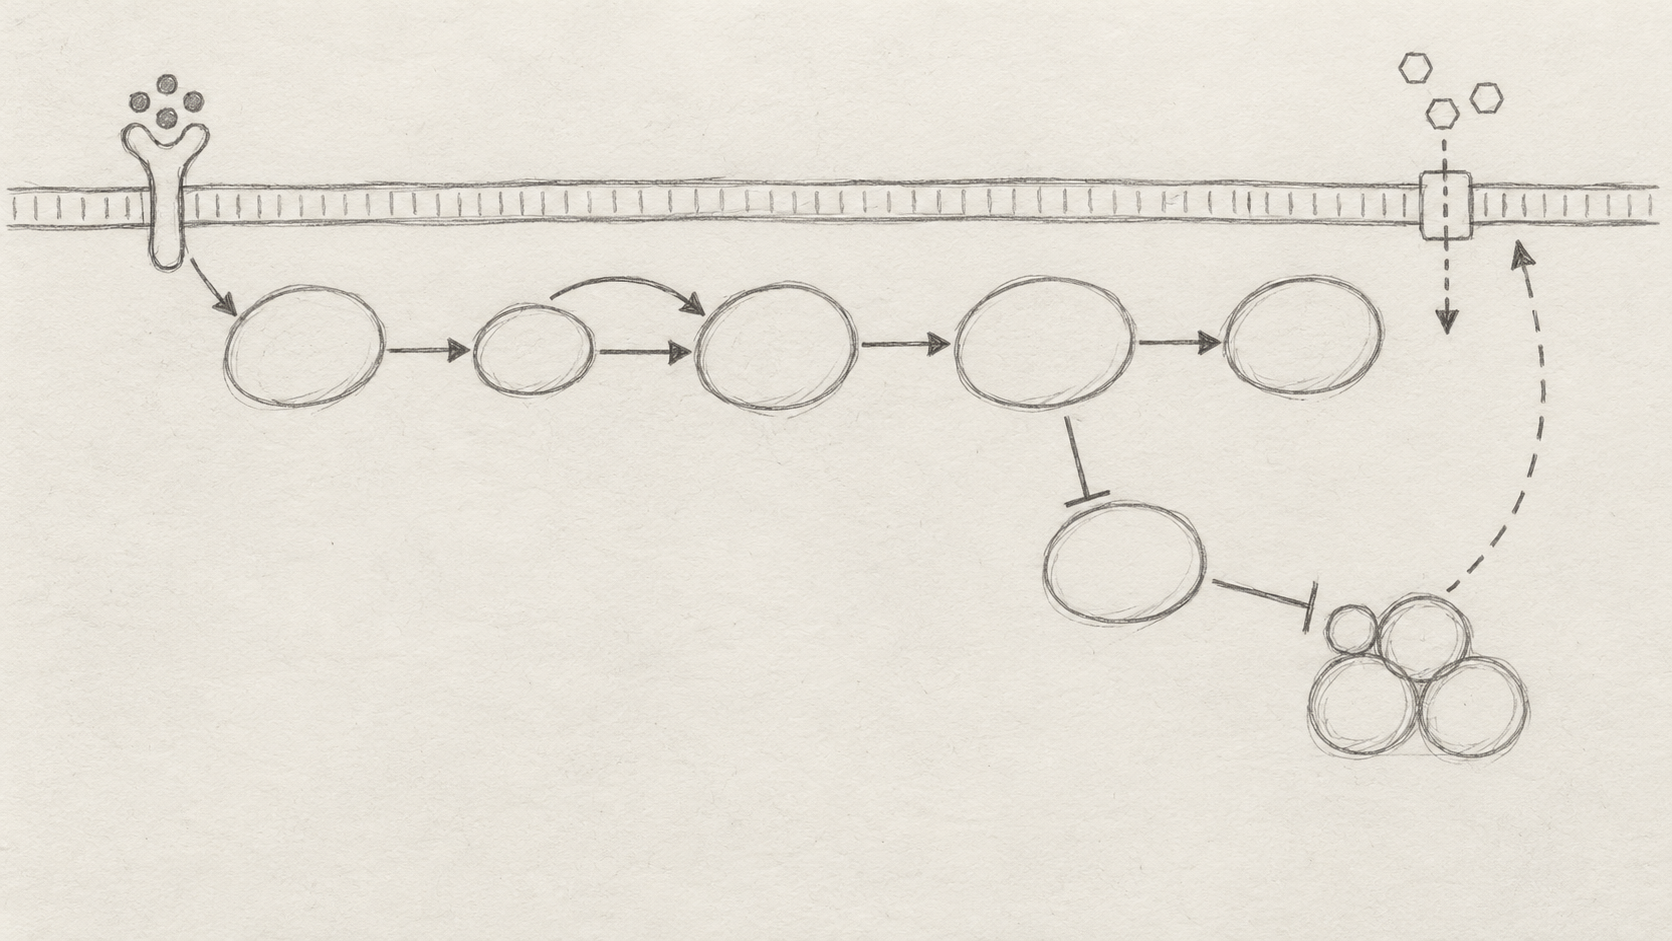
\includegraphics[width=\linewidth]{figures/ch07/ch07-02-v0-sketch.png}};
  \begin{scope}[x={(img.south east)}, y={(img.north west)}]
    \node at (0.12, 1-0.10) {\chsevenrelmark{1}};
    \node at (0.12, 1-0.28) {\chsevenrelmark{2}};
    \node at (0.17, 1-0.44) {\chsevenrelmark{3}};
    \node at (0.25, 1-0.42) {\chsevenrelmark{4}};
    \node at (0.37, 1-0.26) {\chsevenrelmark{5}};
    \node at (0.47, 1-0.37) {\chsevenrelmark{7}};
    \node at (0.53, 1-0.50) {\chsevenrelmark{8}};
    \node at (0.58, 1-0.46) {\chsevenrelmark{9}};
    \node at (0.67, 1-0.58) {\chsevenrelmark{10}};
    \node at (0.80, 1-0.45) {\chsevenrelmark{11}};
    \node at (0.87, 1-0.24) {\chsevenrelmark{12}};
    \node at (0.88, 1-0.12) {\chsevenrelmark{13}};
    \node at (0.44, 1-0.36) {\chsevenrelmark{6}};
  \end{scope}
\end{tikzpicture}

\caption{根据关系表安排布局的手绘草图（图像模型模拟的铅笔草图，非真实手稿）。圆圈编号对应表~\ref{tab:ch07-01} 的关系 R1–R13。草图只确定分区、对象大致位置与阅读路径，不承担对象名称；以草图作为生成输入时，它是布局意图而非布局锁定。}\label{fig:ch07-02}
\end{figure}

图~\ref{fig:ch07-02} 的底图由图像模型模拟铅笔草图生成，圆圈编号 ①–⑬ 在排版阶段用 TikZ 叠加。即便只是生成这样一张构图草图，把同一段提示词连续生成三次，前两次结果都只画了一条 T 形抑制线，且把右下方的囊泡节点与主链断开；第三次生成时专门追加了“必须画出两条串联 T 形抑制线连至囊泡表面小珠”的指令，才得到图~\ref{fig:ch07-02} 中 ⑨ 与 ⑩ 串联的结构。但与此同时，模型把 Akt 下方原本向上指的 mTORC2 团块省去了，反而在主链右侧多画了一个团块；右侧葡萄糖穿膜线（⑬）也画成了短虚线而非点线，左侧配体圆点（①）与受体之间留有小隙。

这正好说明草图的定位：草图不写分子名，只帮作者和工具理顺空间分区与流向。在 SciDraw AI 中，作者可把草图上传至“草图模式”，配合文字任务书生成初稿。但草图约束只是构图意图，不等于硬性的“对象锁定”或布局保持，生成后仍须按表~\ref{tab:ch07-01} 逐行核查。

\section{一句话提示词为什么不够}

为了对比输入完整度对结果的决定性影响，我们把开篇的一句话提示词（V1）与完整任务书驱动的提示词（V2）放进同一环境，并排检验实际产出（图~\ref{fig:ch07-03}）。

在 SciDraw AI 中，建议先打开科研绘图向导（\sdtool{figure-workflow}），选择“机制图与流程图”路线，把默认任务书替换为结构化任务书并下载副本，再进入机制图生成（\sdtool{mechanism-figure-generator}）或提示词绘图（\sdtool{ai-drawing}）。向导只负责组织任务书和串联工具，不会自动检查科学关系。本案例任务书的关键部分如下（完整提示词见本书仓库 \texttt{cases/} 目录）：

\begin{Prompt}
【用途与目标】论文 Figure 1 背景机制图（双栏宽 174 mm）；交代胰岛素经 IR → IRS-1 →
PI3K → PIP3 → Akt 的级联、Akt ⊣ AS160 ⊣ Rab 的双重抑制，以及 GSV 转位融合与葡萄糖内流。
【对象与计数】每个对象只出现一次（GLUT4 除外）：胞外为胰岛素、葡萄糖；质膜为脂双层、
胰岛素受体、内叶 PIP2/PIP3、膜上 GLUT4；胞质为 IRS-1、PI3K、PDK1、Akt、mTORC2、
AS160、囊泡表面 Rab、嵌有 GLUT4 的储存囊泡簇（GSV）。受体、IRS-1、Akt、AS160 标磷酸化圆点。
【关系与线型】R1 胰岛素接触受体（无箭头）；R2 受体自身磷酸化（2 圆点）；R3 受体 → IRS-1、
R4 IRS-1 → PI3K、R7 PDK1 → Akt、R8 mTORC2 → Akt 均为实线实心激活箭头（mTORC2 无上游线）；
R5 PI3K 催化 PIP2 → PIP3 为细弧空心 V 头（PI3K 短线触弧中点）；R6 PIP3 贴膜招募 PDK1 与 Akt；
R9 Akt ⊣ AS160、R10 AS160 ⊣ Rab 均为 T 形抑制线；R11–R12 GSV 向质膜 GLUT4 转位融合为
橙色粗虚线空心箭头；R13 葡萄糖穿过膜 GLUT4 进入胞质为深橙点线箭头。
【布局与视觉】16:9 横幅；上方 20% 胞外、20–28% 质膜、下方胞质、底部 10% 留空给图例。
白底扁平二维矢量风格，无渐变、阴影或 3D；信号蛋白中等蓝，AS160/Rab 灰蓝，GLUT4/GSV/葡萄糖
柔和橙色，膜浅暖灰，磷酸化琥珀色圆点。
【限制】底图不出现任何文字、字母或数字；不画细胞核、内质网、细胞骨架或 MAPK 等旁路。
\end{Prompt}

反例 V1 提交的英文提示词只有一句话：

\begin{Prompt}
Make a beautiful, professional scientific illustration of insulin signaling and
GLUT4 translocation for a top journal.
\end{Prompt}

正例初稿 V2 则将任务书转为结构化英文提示词，明确空间比例（\texttt{SPACE}）、十三个对象的形状与位置（\texttt{OBJECTS}）、五种线型（\texttt{RELATIONS}）和禁画清单（\texttt{DO NOT DRAW}），并要求全图无任何文字（完整提示词见本书仓库 \texttt{cases/} 目录，关键部分如下）：

\begin{Prompt}
Flat 2D scientific schematic for a journal figure, landscape 16:9, pure white
background. Clean vector style, flat fills, thin dark outlines, no gradients,
no shadows, no 3D. ABSOLUTELY NO TEXT: no letters, words, numbers, or symbols.
SPACE: Top 20% = extracellular; 20-28% = horizontal lipid bilayer membrane;
28-88% = cytoplasm; bottom 12% = empty white strip reserved for legend.
OBJECTS (each appears once; GLUT4 appears in vesicles and in plasma membrane):
1. Insulin (3 dark-blue beads touching receptor); 2. Transmembrane receptor (2 amber dots);
3. IRS-1 (1 amber dot); 4. PI3K; 5. Inner-leaflet PIP2 & PIP3; 6. PDK1 & 7. Akt
   (both touching inner leaflet at PIP3; Akt has 2 amber dots); 8. mTORC2 below Akt;
9. AS160 (gray-blue, 1 amber dot); 10. GSV cluster (3 vesicles with orange GLUT4 barrels);
11. Rab bead on vesicle; 12. GLUT4 in right plasma membrane; 13. Glucose hexagons above it.
RELATIONS (draw only these):
- Activation (solid dark-gray line, filled triangle): IR -> IRS-1 -> PI3K; PDK1 -> Akt; mTORC2 -> Akt.
- Inhibition (solid dark-gray line, perpendicular T-bar): Akt -| AS160; AS160 -| Rab.
- Enzymatic conversion (thin mid-gray arc, open V head): PIP2 -> PIP3, PI3K stub touching midpoint.
- Translocation (thick dashed orange arrow, open head): GSV cluster upward to membrane GLUT4.
- Substance flow (dotted dark-orange arrow): extracellular glucose through membrane GLUT4 into cell.
\end{Prompt}

\begin{figure}[htbp]\centering
% FIG ch07-03a V1 error markers (language-neutral)
\definecolor{ch07err}{HTML}{C0392B}
\makeatletter
\@ifundefined{chsevenerrmark}{%
\newcommand{\chsevenerrmark}[2][]{%
  \tikz[baseline=(char.base)]{%
    \node[shape=circle, fill=ch07err, text=white, inner sep=1.5pt,
      font=\fontsize{7}{7}\selectfont\bfseries, #1] (char) {#2};}}%
}{}
\makeatother
\begin{tikzpicture}
  \node[anchor=south west, inner sep=0] (img) at (0,0)
    {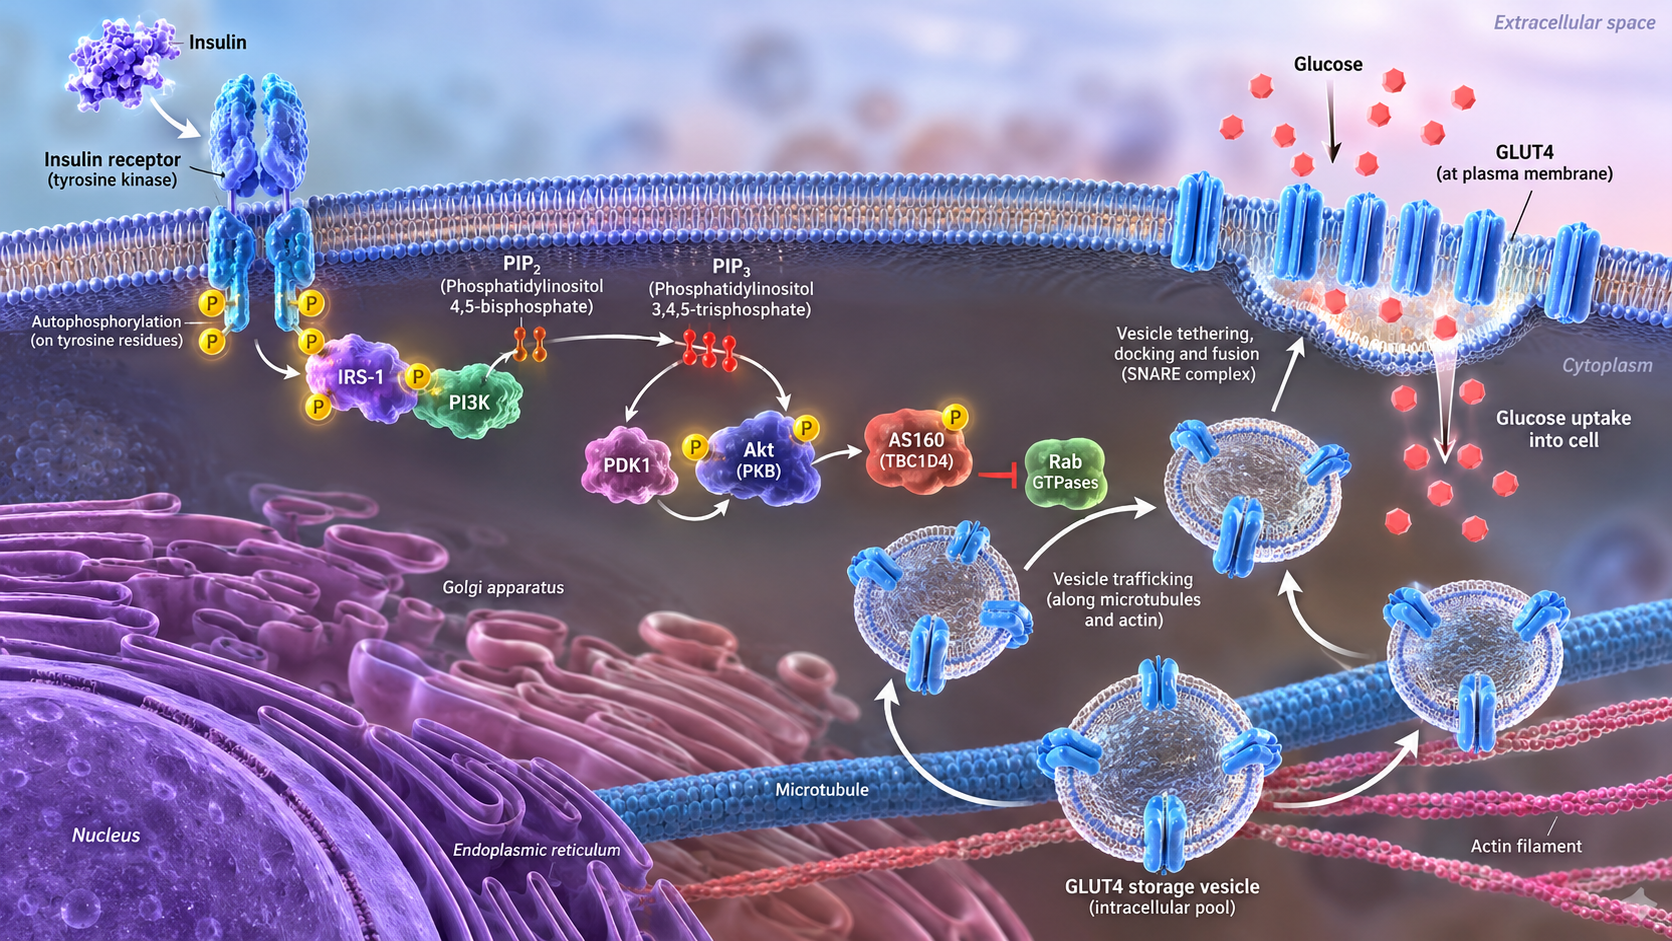
\includegraphics[width=\linewidth]{figures/ch07/ch07-03a-v1-vague.png}};
  \begin{scope}[x={(img.south east)}, y={(img.north west)}]
    \node at (0.14, 1-0.18) {\chsevenerrmark{1}};
    \node at (0.72, 1-0.22) {\chsevenerrmark{2}};
    \node at (0.50, 1-0.35) {\chsevenerrmark{3}};
    \node at (0.38, 1-0.55) {\chsevenerrmark{4}};
    \node at (0.55, 1-0.72) {\chsevenerrmark{5}};
    \node at (0.22, 1-0.48) {\chsevenerrmark{6}};
    \node at (0.82, 1-0.40) {\chsevenerrmark{7}};
  \end{scope}
\end{tikzpicture}


\vspace{2mm}
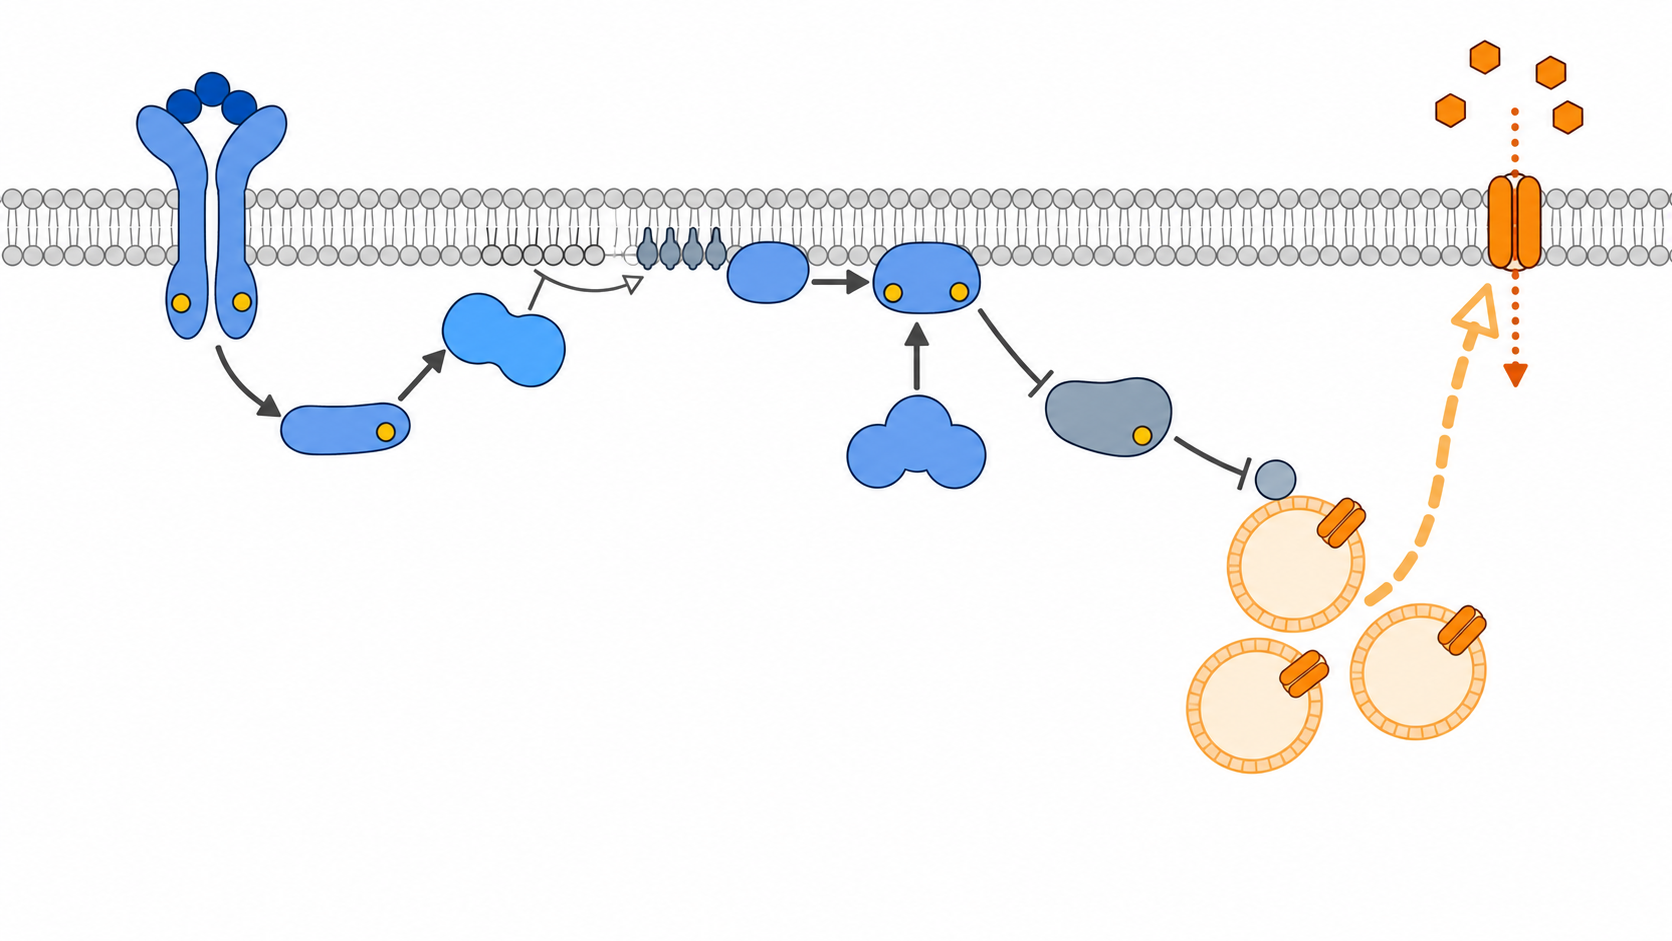
\includegraphics[width=\linewidth]{figures/ch07/ch07-03b-v2-brief.png}
\caption{一句话提示词与完整任务书的生成结果对照。（a）只用一句话提示词生成的初稿；模型把文字直接烤入深色背景，红色编号对应正文列出的问题。（b）使用完整任务书生成的无字初稿：对象与关系基本可逐条核对，配色、线宽与留白尚未统一。本章示例图由图像模型生成，提示词与生成记录见本书仓库。}\label{fig:ch07-03}
\end{figure}

检查图~\ref{fig:ch07-03}a 时可以看到：模型不仅直接把英文标签烤进了位图，而且在缩至 174 mm 通栏印刷宽度后，深色三维背景与发光特效上的小字难以辨认，后期也无法单独调整字号或改正拼写。更重要的是，对照表~\ref{tab:ch07-01} 逐项核查，这张看似华丽的初稿存在七处明显问题（对应图~\ref{fig:ch07-03}a 的红色编号 ❶–❼）：
\begin{enumerate}
\item \textbf{配体结合方式与 3D 装饰过度（❶）：} 胞外胰岛素到受体画了白色箭头而非直接接触（违反 R1）；蛋白带强烈高光、阴影与发光“P”球，干扰边界识别。
\item \textbf{膜上对象重复与文字堆砌（❷）：} 右上质膜凹坑内并排塞进六个蓝色 GLUT4 通道（违反唯一计数），并在胞质中印上三行关于 SNARE 的描述性文字。
\item \textbf{核心关系反转、缺支路与位置错误（❸）：} 首先，\textbf{mTORC2 完全缺失}（缺 R8）。其次，\textbf{Akt 到 AS160 被画成白色实心激活箭头}（R9 错误），而 AS160 到 Rab 画了红色 T 形抑制线（R10）——串起来读竟变成“Akt 激活 AS160 进而抑制 Rab”，与生物学事实完全相反！此外，$\text{PIP}_3$ 用箭头连向远离质膜的 PDK1 与 Akt（违反 R6 贴膜要求），绿色的 Rab 游离在胞质中而未附着囊泡表面。
\item \textbf{无关细胞器占据半幅画面（❹）：} 左下绘出巨大的细胞核、内质网和高尔基体，挤占了信号主干空间。
\item \textbf{细胞骨架与循环弯箭头造成歧义（❺）：} 右下画出微管与肌动蛋白丝，四个剖面囊泡由弯箭头连成环路，分不清储存池与转位方向。
\item \textbf{上游蛋白重叠与催化连接错误（❻）：} IRS-1 与 PI3K 直接重叠，缺少激活箭头（R4 不清）；PI3K 指向 $\text{PIP}_2$ 本身而非转化弧中点（R5 错误）。
\item \textbf{箭头同型且无图例（❼）：} 除一处红 T 端外，结合、催化、激活、囊泡移动和葡萄糖内流全用白色实心箭头，且无图例。
\end{enumerate}

为什么 Akt 抑制 AS160（R9）与 AS160 抑制 Rab（R10）这段“抑制的抑制”必须保留两条串联 T 形线？基础状态下，AS160 具有 GAP 活性，促使 Rab 水解 GTP 变为失活态，像刹车一样把囊泡扣留在胞质（Sano 等，2003；Leto 与 Saltiel，2012）。Akt 磷酸化并\textbf{抑制} AS160，相当于松开刹车，使 Rab 维持 GTP 结合态并推动囊泡转位。如果省成“Akt $\rightarrow$ GSV”一条大箭头，就抹去了可核对的机制节点；如果像图~\ref{fig:ch07-03}a 那样画成一激活一抑制，则直接画反了因果。

再看按完整任务书生成的图~\ref{fig:ch07-03}b。把同一提示词生成两次时，第一张候选图曾把本应指向 AS160 的 T 形线错接到 mTORC2 上，并在囊泡表面画了两颗 Rab 珠；第二张候选图（图~\ref{fig:ch07-03}b）纠正了这一连接。图中“胞外—质膜—胞质”三分区清楚，十三个对象计数、六枚琥珀色磷酸化圆点及五类线型全部到位，无多余细胞器或文字。这证明结构正确主要取决于输入任务书的完整度，同时每次生成仍须逐条核对连接点。

\section{线型与颜色：只让它们承担一种含义}

拿到结构初稿后，修改阶段最容易出现两类偏差：一是随意变换箭头的线型、粗细和颜色；二是给每个蛋白涂上高饱和度的不同颜色。下面通过两组对照图说明视觉规范。

第一组对照（图~\ref{fig:ch07-04}）截取“Akt $\dashv$ AS160 $\dashv$ Rab $\rightarrow$ 囊泡转位至膜 GLUT4”局部。图~\ref{fig:ch07-04}a 故意混用四种线：蓝椭圆到灰蓝团块用粗红实心弯箭头（把抑制画成激活），灰蓝团块到囊泡小珠用细绿虚线空心头，囊泡簇到膜转运体用与普通激活相同的黑色实线实心箭头（让人误以为囊泡“激活”了 GLUT4），蓝椭圆与质膜间还多出一条含义不明的紫色双向箭头。图~\ref{fig:ch07-04}b 则只用三条线、两种线型：两条等粗深灰 T 形线串联表示双重抑制，唯一一条柔和橙色粗虚线空心头向上表示空间转位（放大检查仍可见 T 端留有微隙、蛋白带轻微渐变）。无需文字，读者也能从图~\ref{fig:ch07-04}b 区分负调控信号与空间移动。

\begin{figure}[htbp]\centering
\begin{minipage}[t]{0.48\linewidth}\centering
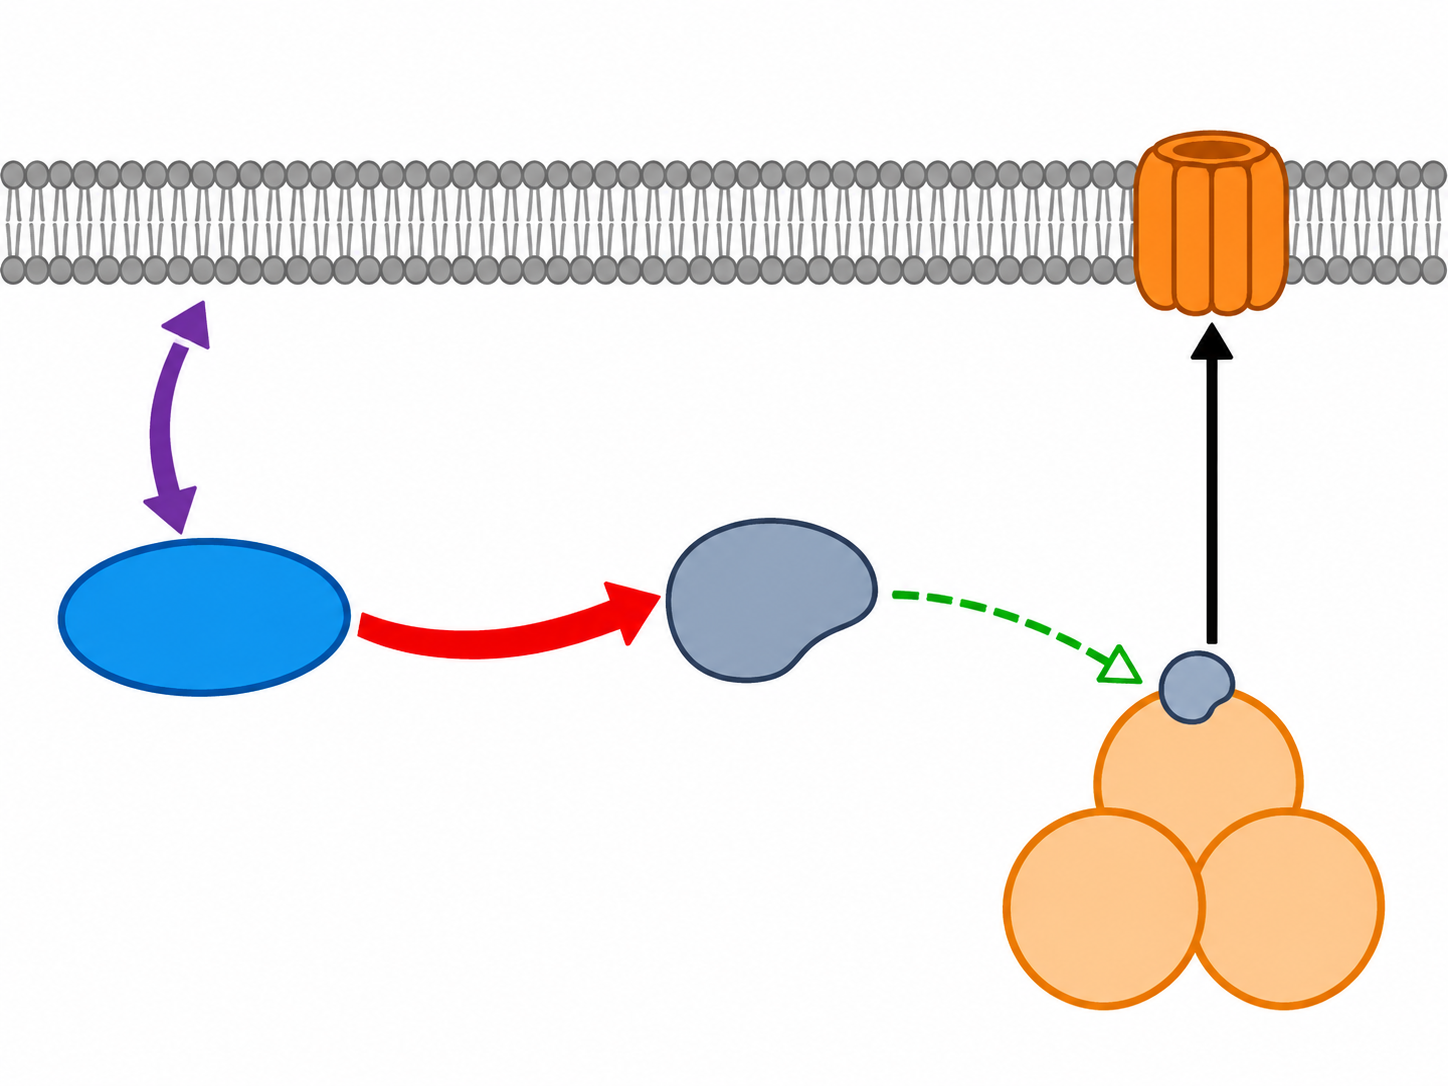
\includegraphics[width=\linewidth]{figures/ch07/ch07-04a-mixed-arrows.png}\\[1mm]
{\footnotesize (a) 线型混用：抑制、转位与双向箭头混淆}
\end{minipage}\hfill
\begin{minipage}[t]{0.48\linewidth}\centering
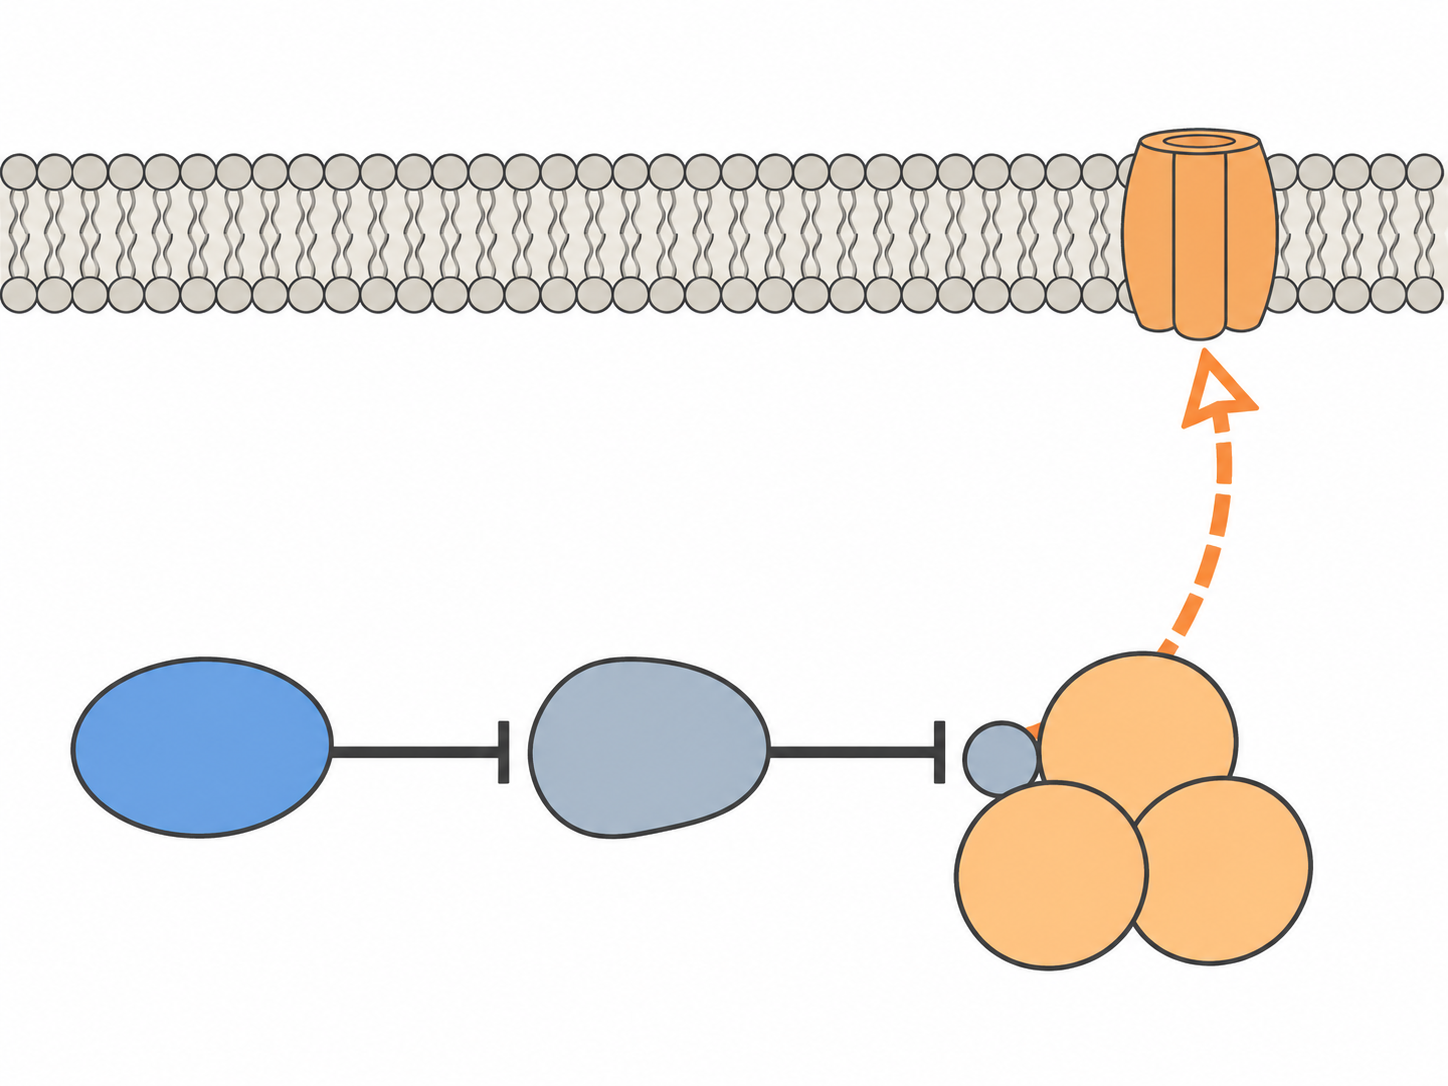
\includegraphics[width=\linewidth]{figures/ch07/ch07-04b-unified-arrows.png}\\[1mm]
{\footnotesize (b) 线型统一：两条串联 T 形线与粗虚线转位}
\end{minipage}
\caption{同一段简化通路的两种画法。（a）线型、颜色和粗细随意变化，转位箭头与激活箭头同型，另有一条含义不明的双向箭头。（b）两条 T 形线串联表示“抑制的抑制”，粗虚线是唯一的空间转位符号。}\label{fig:ch07-04}
\end{figure}

第二组对照（图~\ref{fig:ch07-05}）比较配色过多与配色克制，并展示灰度测试结果。

\begin{figure}[htbp]\centering
\begin{minipage}[t]{0.48\linewidth}\centering
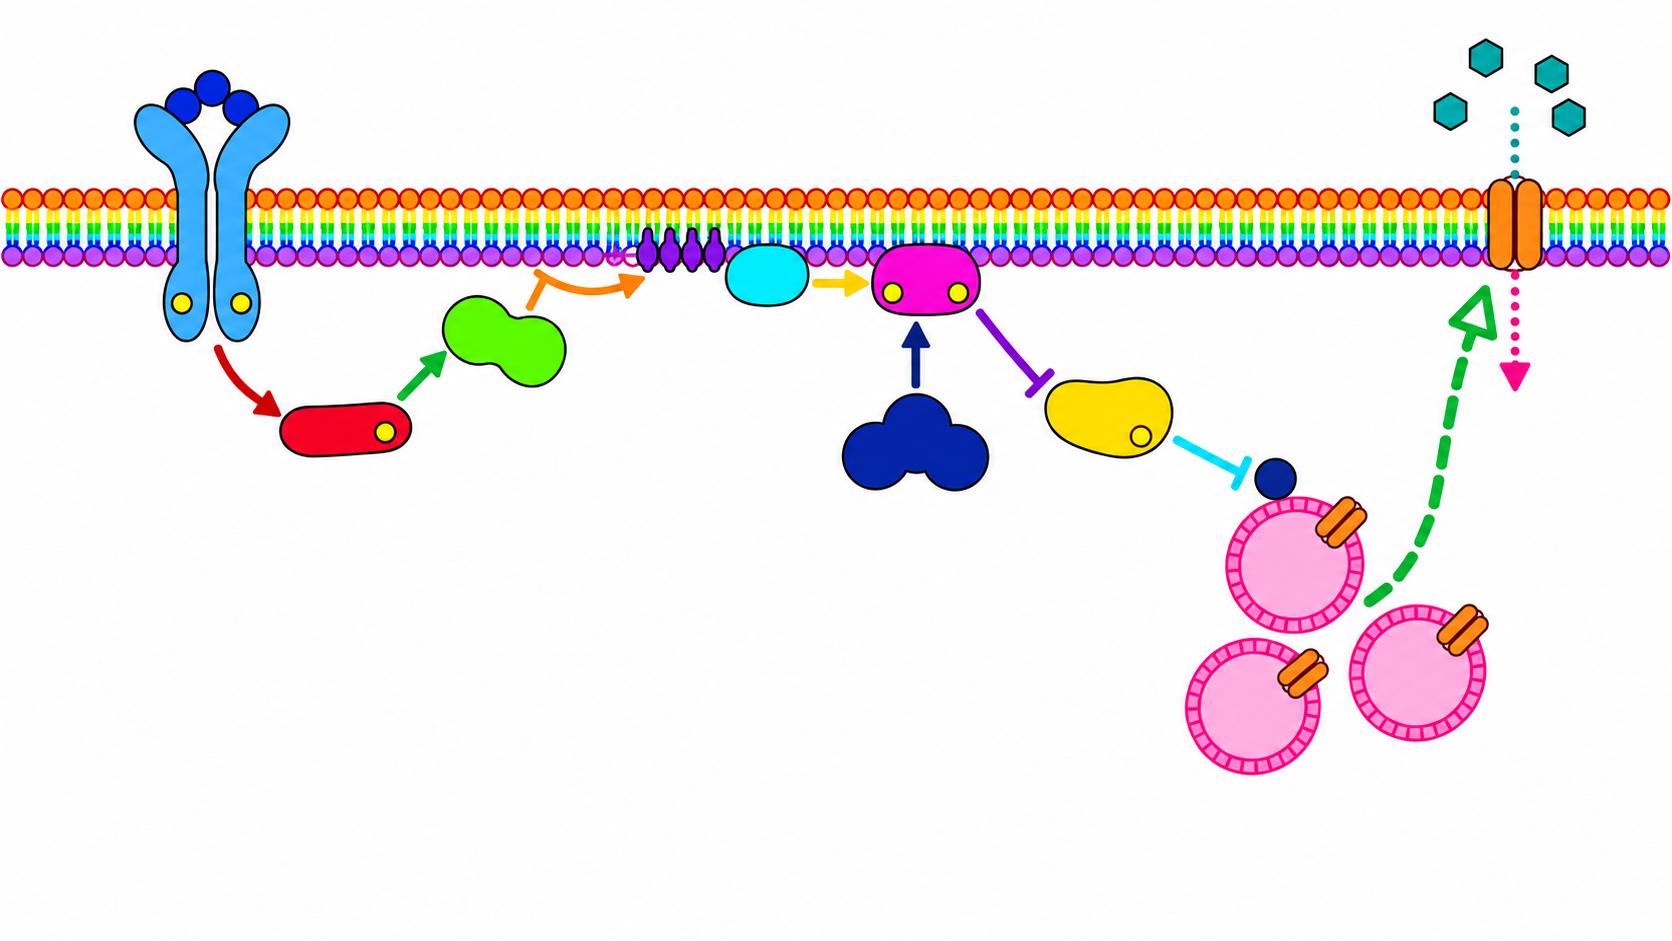
\includegraphics[width=\linewidth]{figures/ch07/ch07-05a-many-colours.png}\\[1mm]
{\footnotesize (a) 配色过多：每蛋白异色与彩虹膜}
\end{minipage}\hfill
\begin{minipage}[t]{0.48\linewidth}\centering
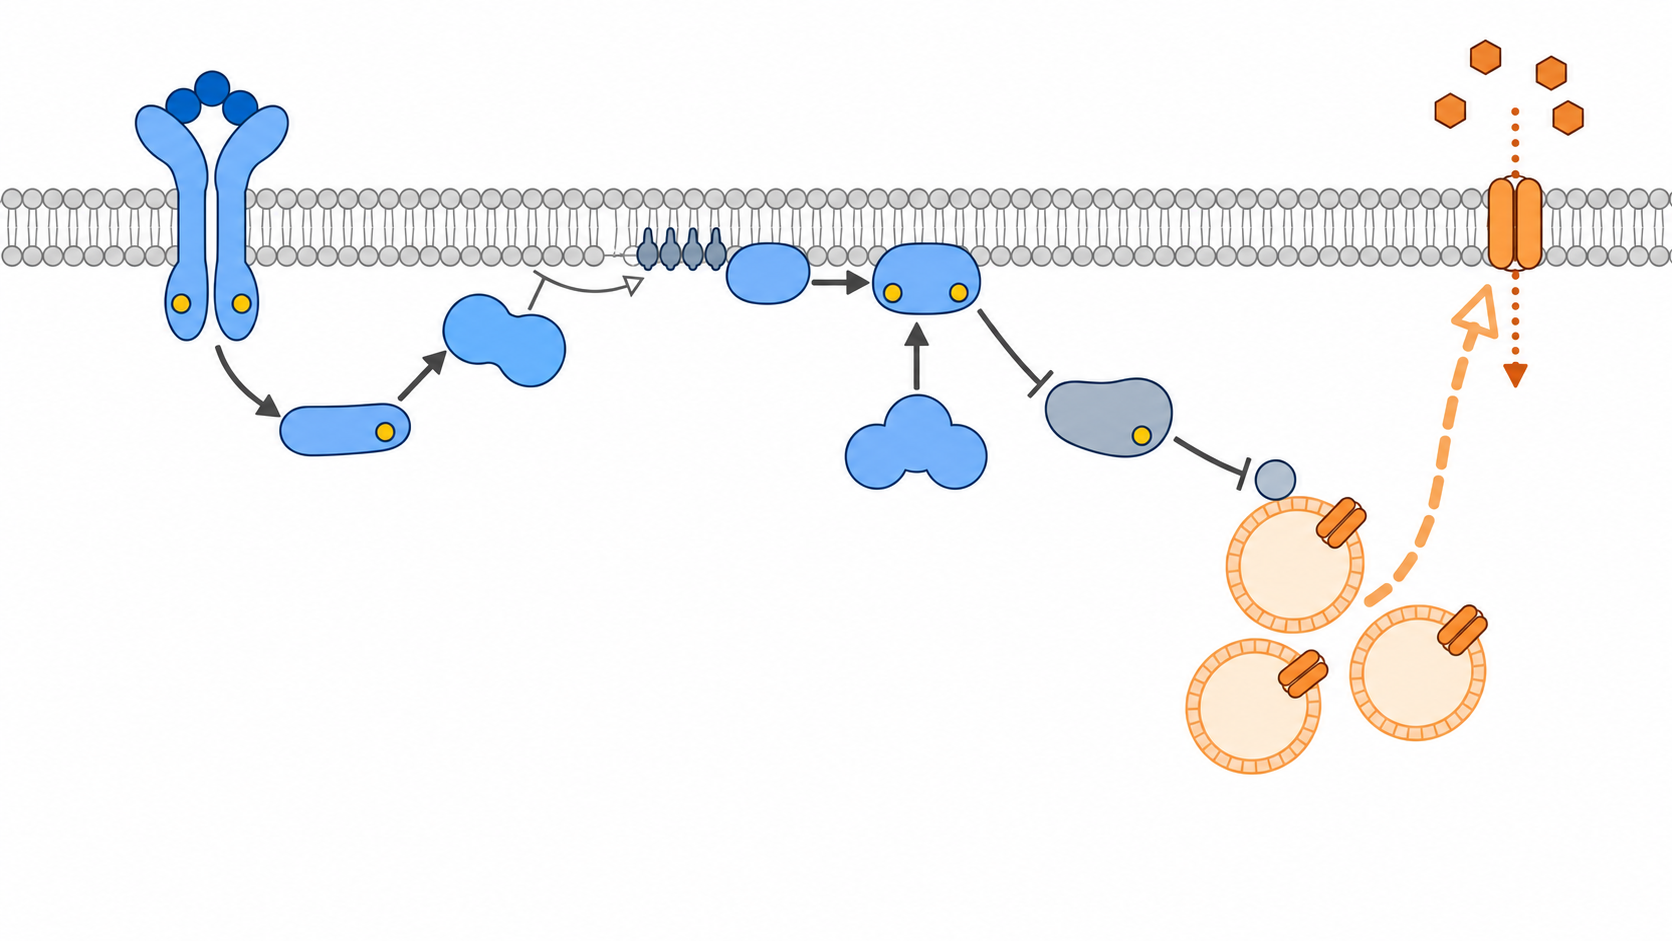
\includegraphics[width=\linewidth]{figures/ch07/ch07-05b-v3-revised.png}\\[1mm]
{\footnotesize (b) 配色克制（V3）：三种角色色相加灰}
\end{minipage}

\vspace{2mm}
\begin{minipage}[t]{0.48\linewidth}\centering
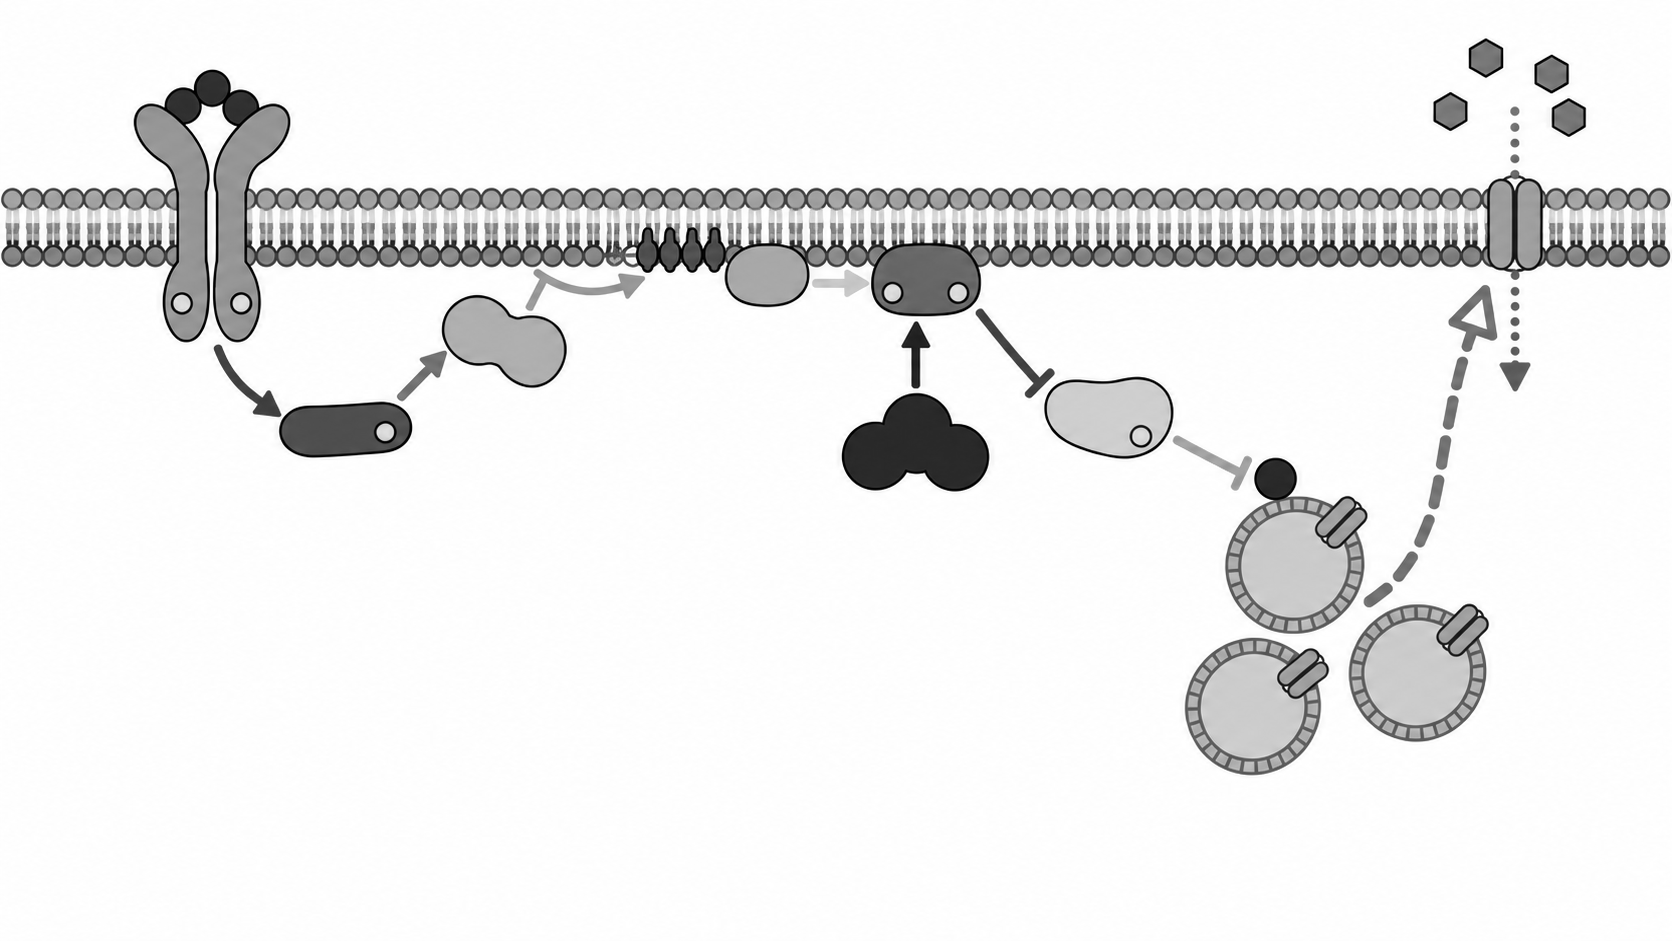
\includegraphics[width=\linewidth]{figures/ch07/ch07-05a-many-colours-gray.png}\\[1mm]
{\footnotesize (c) 图 (a) 的灰度转换结果}
\end{minipage}\hfill
\begin{minipage}[t]{0.48\linewidth}\centering
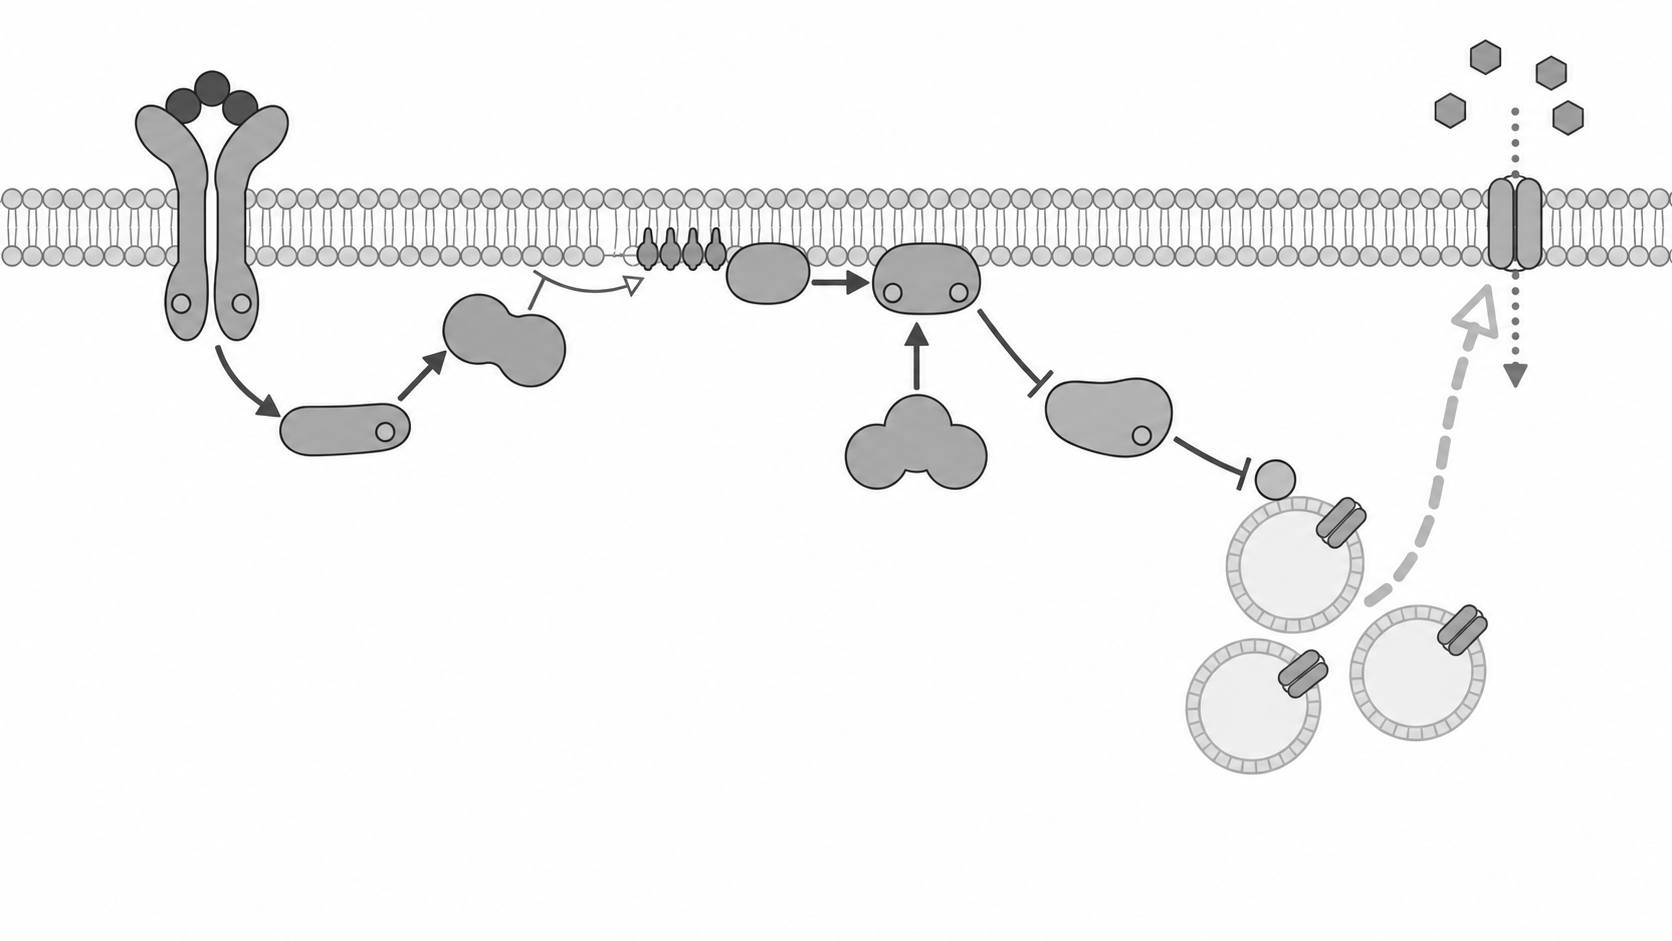
\includegraphics[width=\linewidth]{figures/ch07/ch07-05b-v3-revised-gray.png}\\[1mm]
{\footnotesize (d) 图 (b) 的灰度转换结果}
\end{minipage}
\caption{机制图的配色对比与灰度测试。（a）每个蛋白一种饱和色、彩虹色膜，颜色不承担含义。（b）修订稿（V3）只用三种色相加灰色，分别对应信号蛋白、运输调控蛋白、运输物质及其载体。下行为两图的灰度版本：（b）的层级与线型在灰度下仍可辨认。}\label{fig:ch07-05}
\end{figure}

生成图~\ref{fig:ch07-05}a 的过程同样说明了模型的不稳定性：第一次在不带参考图的情况下要求“每个蛋白涂不同颜色、质膜涂成彩虹色”时，模型为了迎合花哨配色，竟把整条通路改写成了单条六蛋白激活链，丢掉了两条 T 形抑制线和 mTORC2，还把葡萄糖跨膜箭头画反；第二次以图~\ref{fig:ch07-05}b 作参考图才保住主体布局，但 $\text{PIP}_2 \rightarrow \text{PIP}_3$ 转化弧的箭头仍意外由空心变成了实心。

对比图~\ref{fig:ch07-05}a 与 b 可以看出三点原则（Rougier 等，2014；Wong，2011）：第一，颜色应只编码功能角色。图~\ref{fig:ch07-05}a 中蛋白涂成红、亮绿、青、洋红、深蓝、明黄，读者找不到分组依据（如 mTORC2 与 Rab 同为深蓝却无关联）；图~\ref{fig:ch07-05}b 则只用三个色相——正向信号蛋白统一中等蓝，负调控与运输开关（AS160、Rab）统一低饱和灰蓝，被转运物质与载体（葡萄糖、GLUT4、囊泡）统一柔和橙色，质膜用浅暖灰。第二，避免红绿并用。图~\ref{fig:ch07-05}a 中红绿蛋白与红绿箭头相邻，对红绿色觉差异读者不友好（Wong，2011；选色可借助 ColorBrewer 2.0）。第三，通过灰度测试检验层级。将彩图转为灰度后，图~\ref{fig:ch07-05}c 的彩虹膜沉重刺眼、各蛋白明度杂乱；而图~\ref{fig:ch07-05}d 中同类蛋白明度一致，五种线型依靠实线、T 端、细弧、粗虚线和点线的几何形状依然可辨（同时可见橙色粗虚线转灰后偏浅，提示终稿可在虚线旁加文字辅助）。作者可用 SciDraw AI 的“图片检查”（\sdtool{figure-checker}）检查灰度与色觉风险，但须知它只是技术检查，无法判断科学关系正误。

\section{主案例：从修订到终稿}

下面梳理主案例从 V2 初稿（图~\ref{fig:ch07-03}b）到 V3 修订稿（图~\ref{fig:ch07-05}b）、再到 V4 终稿（图~\ref{fig:ch07-06}）、图注与核验的完整闭环。

\subsection{从 V2 到 V3：修改指令与“意外变化”的拦截}

对照表~\ref{tab:ch07-01} 核查 V2 初稿（图~\ref{fig:ch07-03}b），其主干拓扑与对象数正确，但放大检查仍可见五处具体偏差：（1）PI3K 催化 $\text{PIP}_2 \rightarrow \text{PIP}_3$ 的转化弧（R5）画成了闭合空心三角头而非开放 V 头，且 PI3K 催化短线接在弧线左端而非中点；（2）膜招募环节（R6）中 Akt 离质膜内叶 $\text{PIP}_3$ 头基稍远；（3）双重抑制环节（R9、R10）的 T 形端与靶标之间、以及囊泡转位箭头终点（R12）与膜上 GLUT4 之间留有窄白隙；（4）蛋白填充仍有轻微明暗渐变；（5）局部留白偏紧，直接叠加文字容易压住图形边缘，且底图在 174 mm 通栏宽度下折算分辨率约 244 ppi，尚未达到期刊常见的 300 ppi 印刷要求。

推进到 V3 时，修改指令先写“保持不变”的部分，再逐条写可核对的改动：

\begin{Prompt}
保持所有对象、位置和 13 条关系不变，只做以下修改：
1. 全部信号蛋白（受体、IRS-1、PI3K、PDK1、Akt、mTORC2）改为同一种中等蓝填充、同一深灰描边；
   AS160 与 Rab 改为同一种低饱和灰蓝。
2. 所有激活箭头与抑制线统一为同一粗细；抑制端统一为垂直短横线并紧贴靶标轮廓。
3. 酶促转化弧线改细、改为中灰开放 V 形头，PI3K 短线接触弧线中点，与激活箭头明显区分。
4. 胰岛素与葡萄糖保持约为蛋白的 1/3；GSV 簇清晰可辨。
5. 每个对象四周留出至少一个对象宽度的空白；底部 12% 清空；全图无任何文字。
\end{Prompt}

生成 V3 的两次尝试给出了关于“意外变化”的重要教训：第一次不带参考图直接按修订后的完整提示词重新生成时，模型弄丢了全部磷酸化圆点，把胰岛素减为 2 颗且脱离受体，让 PDK1 与 Akt 脱离质膜，在 PI3K 与 PDK1 之间凭空添了一条实心激活箭头，还把每个囊泡上的 GLUT4 画成了多个！第二次改以 V2 初稿作为参考图配合上述修改指令修订（得到图~\ref{fig:ch07-05}b），模型完整保住了十三个对象、六枚磷酸化点、贴膜关系与五类线型，未添多余箭头；代价是色彩明暗、PI3K 催化短线偏左与 T 端微隙改善有限。这说明：**每次修改后都必须重做全表复核，绝不能只看要求修改的那一处。**

\subsection{V4 终稿：无字底图加 LaTeX/TikZ 叠加层}

为什么终稿坚持“无字底图 + LaTeX/TikZ 叠加标签”？因为图像模型拼写分子名不可靠（如把 \texttt{Akt} 拼成 \texttt{Act} 即成科学错误），字号不可控，且每次生成位置漂移。把文字放到 TikZ 中，拼写可直接从清单复制，印刷字号精确控制在 7–8 pt，且中英文两版可以共用同一张无字底图，只需切换叠加层的语言文本。交付时可走\textbf{方案 A}（底图含对象与箭头，TikZ 只叠文字和图例，本例采用）或\textbf{方案 B}（底图只画对象，箭头也由 TikZ 绘制，下一节电池案例采用）。

以 V3 为参考生成 V4 底图时，提示词进一步锁定了色板与标签留白区（完整提示词见本书仓库 \texttt{cases/} 目录）：

\begin{Prompt}
Final base artwork for a journal Figure 1, flat 2D vector-style scientific
schematic, landscape 16:9, print resolution 300 ppi at 174 mm width, pure white
background, uniform thin dark gray (#3A3A3A) outlines, flat fills, no gradients.
THIS IMAGE MUST CONTAIN NO TEXT AT ALL: no letters, words, numbers, or "P".
PALETTE: signaling proteins #A9C4E0 / #4C78A8; insulin #2F5D8C; AS160 and Rab
#B8C2CC; GLUT4 and vesicles #F2C49B / #E39B5B; glucose #C46A2A; membrane
#D9D6D0 / #BDB8AF; phosphorylation dots #E3B23C; lines #3A3A3A and #7A7A7A.
LAYOUT & RELATIONS: keep the same 13 objects, phosphorylation dots, and 5 line
types as the reference image. Leave generous empty white margins above the
membrane, around each protein, and across the bottom 12% strip for overlaid
labels and the figure legend.
\end{Prompt}

生成 V4 底图时同样经历了从拦截偏差到排版微调的过程：第一次不带参考图生成时，模型曾把囊泡上的 GLUT4 错画进囊泡腔内；改用 V3 作参考图生成的第三次结果恢复了正确的囊泡膜嵌合位置，放大至 200\% 逐区检查确认无任何残余文字或水印。不过，模型生成的图形边缘仍占用了部分预留给文字的空白，PI3K 催化短线接点偏左与 T 形端微隙也依然存在，174 mm 通栏宽度下折算分辨率约 244 ppi。因此，在 LaTeX 中用 TikZ 建立以底图左下角为 $(0,0)$、右上角为 $(1,1)$ 的归一化坐标系后，我们根据底图实际留白微调了十七个标签的位置，在空间紧凑处用短引线避开图形边缘，并在底部空白带排版了矢量图例（图~\ref{fig:ch07-06}）。

\begin{figure}[htbp]\centering
% FIG ch07-06 GLUT4 final overlay (Chinese)
\definecolor{ch07comp}{HTML}{6B6B6B}
\definecolor{ch07transnote}{HTML}{C46A2A}
\definecolor{ch07act}{HTML}{3A3A3A}
\definecolor{ch07conv}{HTML}{7A7A7A}
\definecolor{ch07trans}{HTML}{E39B5B}
\definecolor{ch07flux}{HTML}{C46A2A}
\definecolor{ch07phos}{HTML}{E3B23C}
\begin{tikzpicture}
  \node[anchor=south west, inner sep=0] (img) at (0,0)
    {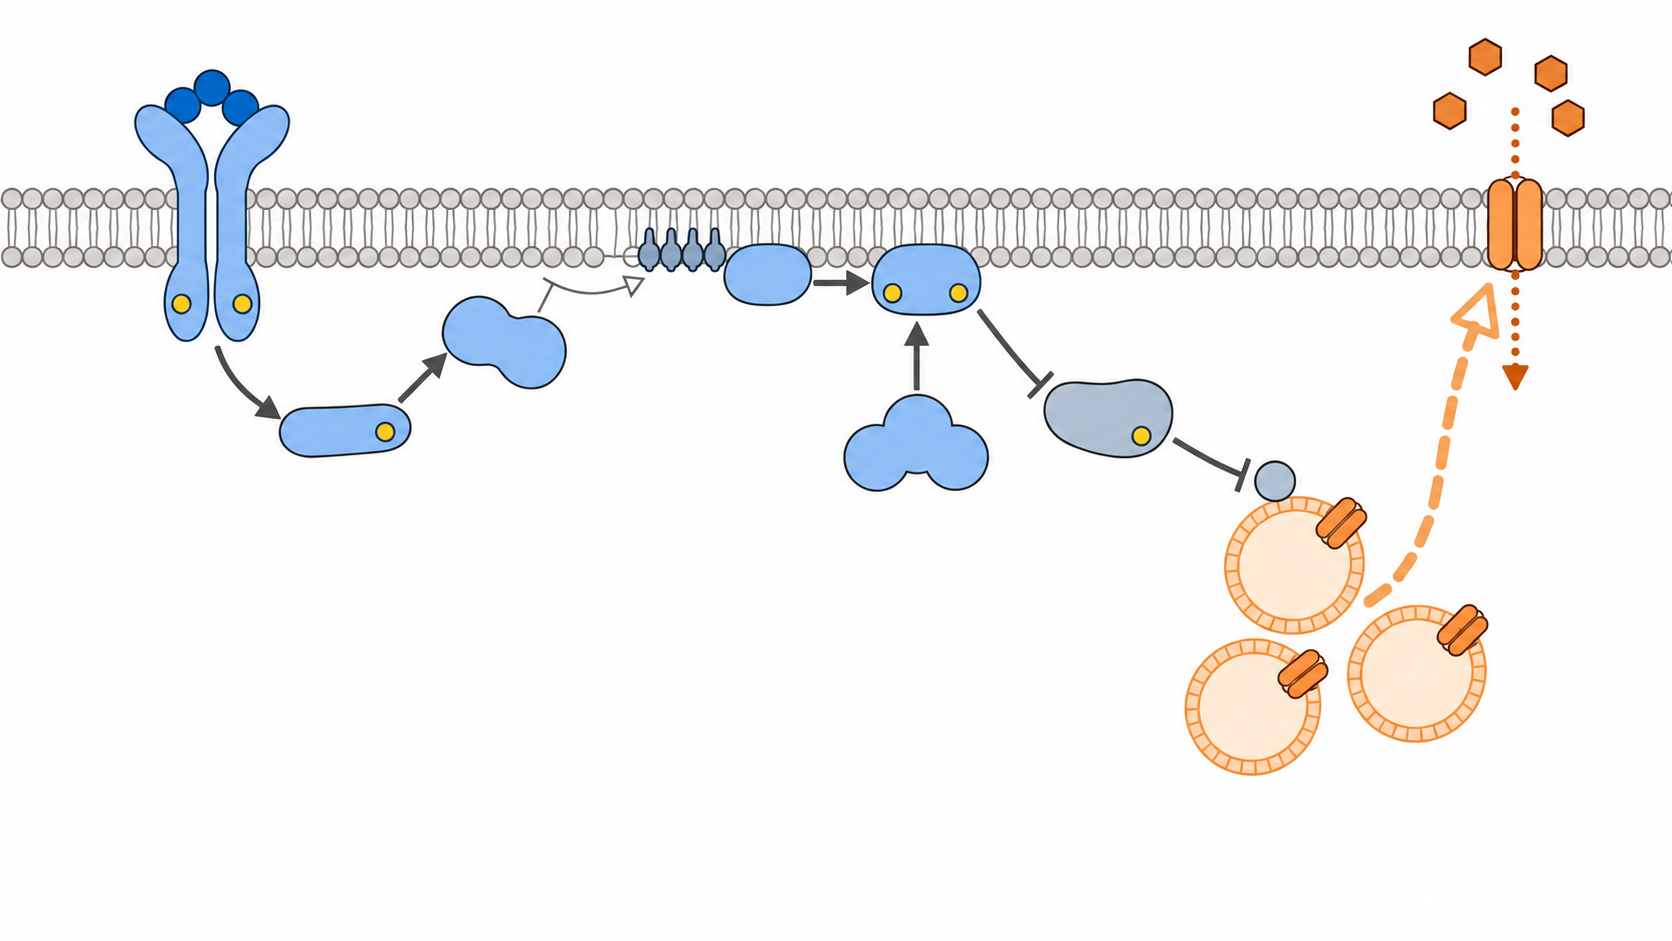
\includegraphics[width=\linewidth]{figures/ch07/ch07-06-v4-base.png}};
  \begin{scope}[x={(img.south east)}, y={(img.north west)},
    font=\sffamily\small]
    \node[text=ch07comp, font=\sffamily\footnotesize\itshape, anchor=west]
      at (0.04, 1-0.055) {胞外};
    \node[text=ch07comp, font=\sffamily\footnotesize\itshape]
      at (0.70, 1-0.15) {质膜};
    \node[text=ch07comp, font=\sffamily\footnotesize\itshape, anchor=west]
      at (0.04, 1-0.90) {胞质};
    \node[anchor=west, font=\sffamily\small] at (0.20, 1-0.06) {胰岛素};
    \draw[BookInk!40, thin] (0.20, 1-0.065) -- (0.145, 1-0.10);
    \node[anchor=west, font=\sffamily\small] at (0.20, 1-0.145) {胰岛素受体};
    \draw[BookInk!40, thin] (0.20, 1-0.15) -- (0.16, 1-0.20);
    \node[font=\sffamily\small] at (0.21, 1-0.56) {IRS-1};
    \node[font=\sffamily\small] at (0.34, 1-0.50) {PI3K};
    \node[font=\sffamily\footnotesize] at (0.47, 1-0.075) {PIP\textsubscript{2} → PIP\textsubscript{3}};
    \draw[BookInk!40, thin] (0.43, 1-0.10) -- (0.385, 1-0.275);
    \node[font=\sffamily\small] at (0.46, 1-0.40) {PDK1};
    \node[font=\sffamily\small] at (0.515, 1-0.375) {Akt};
    \draw[BookInk!40, thin] (0.53, 1-0.36) -- (0.55, 1-0.335);
    \node[font=\sffamily\small] at (0.52, 1-0.60) {mTORC2};
    \draw[BookInk!40, thin] (0.54, 1-0.56) -- (0.55, 1-0.52);
    \node[align=center, font=\sffamily\footnotesize] at (0.785, 1-0.345) {AS160\\（TBC1D4）};
    \draw[BookInk!40, thin] (0.745, 1-0.385) -- (0.695, 1-0.42);
    % Two short lines in the white gap right of the Rab circle (x 0.78–0.84).
    \node[align=left, font=\sffamily\scriptsize, anchor=south west] at (0.788, 1-0.508) {Rab-\\GTP};
    \draw[BookInk!40, thin] (0.784, 1-0.500) -- (0.770, 1-0.512);
    \node[font=\sffamily\small, anchor=north] at (0.78, 1-0.85) {GLUT4 储存囊泡};
    \draw[BookInk!40, thin] (0.78, 1-0.845) -- (0.78, 1-0.80);
    \node[font=\sffamily\small, anchor=west] at (0.94, 1-0.345) {GLUT4};
    \draw[BookInk!40, thin] (0.94, 1-0.33) -- (0.915, 1-0.26);
    \node[font=\sffamily\small, anchor=east] at (0.845, 1-0.065) {葡萄糖};
    \draw[BookInk!40, thin] (0.845, 1-0.075) -- (0.875, 1-0.09);
    % White gap beside the dashed arrow (the dashes sit near x=0.86).
    \node[text=ch07transnote, font=\sffamily\scriptsize\itshape, anchor=east]
      at (0.985, 1-0.455) {转位与融合};
    \draw[ch07transnote!55, thin] (0.876, 1-0.455) -- (0.858, 1-0.432);
  \end{scope}
  \node[anchor=north west, font=\sffamily\scriptsize, align=left] at (img.south west) {%
    \begin{tabular}{@{}l@{\quad}l@{}}
      \tikz{\draw[-{Stealth[length=1.5mm]}, ch07act, line width=0.6pt] (0,0) -- (0.22,0);} 激活 &
      \tikz{\draw[-{Bar[width=4pt]}, ch07act, line width=0.6pt] (0,0) -- (0.22,0);} 抑制 \\
      \tikz{\draw[ch07conv, line width=0.4pt] (0,0) .. controls (0.08,0.04) .. (0.18,0);} 酶促转化 &
      \tikz{\draw[ch07trans, line width=1pt, dashed] (0,0) -- (0.18,0);} 囊泡转位 \\
      \tikz{\draw[ch07flux, line width=0.6pt, dotted, -{Stealth[length=1.2mm]}] (0,0) -- (0.18,0);} 葡萄糖流动 &
      \tikz{\fill[ch07phos] (0.09,0) circle (1.2pt);} 磷酸化
    \end{tabular}};
\end{tikzpicture}

\caption{胰岛素刺激 GLUT4 转位的经典信号通路示意（终稿）。底图由图像模型生成且不含文字，标签与图例由 LaTeX 排版叠加。实线实心箭头表示激活，T 形端表示抑制，细弧线表示酶促转化，粗虚线表示囊泡转位，点线表示葡萄糖流动，琥珀色圆点表示磷酸化。图中省略了 MAPK 与 CAP–Cbl–TC10 分支、GLUT4 内吞与再循环、负反馈、SNARE 融合机器与细胞骨架运输，未区分 Akt 与 Rab 亚型，未画 mTORC2 的上游调控。依据 Saltiel 与 Kahn（2001）、Leto 与 Saltiel（2012）、Klip 等（2019）整理。完整图注见正文。}\label{fig:ch07-06}
\end{figure}

\subsection{完整图注、自查与核验记录}

若使用 SciDraw AI“图注辅助”（\sdtool{figure-legend}）起草图注，只能将其作为初稿，绝不能让工具补写样本量或统计检验。本案例的完整中英文图注如下：

\begin{BookNote}
\textbf{图 1　胰岛素刺激 GLUT4 转位的经典信号通路示意。} 胰岛素与质膜上的胰岛素受体结合，引起受体胞内段酪氨酸自身磷酸化，进而磷酸化 IRS-1 并招募 I A 类 PI3K。PI3K 在质膜内叶将 $\text{PIP}_2$ 转化为 $\text{PIP}_3$，后者招募 PDK1 与 Akt；Akt 由 PDK1 和 mTORC2 磷酸化而激活。活化的 Akt 磷酸化 AS160（TBC1D4），抑制其 Rab-GAP 活性，使 GLUT4 储存囊泡上的 Rab 维持 GTP 结合状态，促进囊泡向质膜转位并融合，GLUT4 由此增加于质膜，葡萄糖经其易化扩散进入细胞。实线实心箭头表示激活，T 形端表示抑制，细弧线表示酶促转化，粗虚线表示囊泡转位，点线表示葡萄糖流动，琥珀色圆点表示磷酸化。为便于阅读，图中省略了 MAPK 与 CAP–Cbl–TC10 分支、GLUT4 内吞与再循环、负反馈调节、SNARE 融合机器及细胞骨架运输；Rab 未区分具体亚型，Akt 未区分亚型，骨骼肌中并行的 TBC1D1 未画出；mTORC2 的上游激活方式未表示。依据 Saltiel 与 Kahn（2001）、Leto 与 Saltiel（2012）、Klip 等（2019）的综述整理。

\medskip
\textbf{Figure 1 | Schematic of the canonical insulin signaling pathway leading to GLUT4 translocation.} Insulin binding to the insulin receptor at the plasma membrane triggers tyrosine autophosphorylation of the receptor's intracellular domain, which phosphorylates IRS-1 and recruits class IA PI3K. PI3K converts $\text{PIP}_2$ to $\text{PIP}_3$ in the inner leaflet; $\text{PIP}_3$ recruits PDK1 and Akt, and Akt is activated by phosphorylation by PDK1 and mTORC2. Active Akt phosphorylates AS160 (TBC1D4), inhibiting its Rab-GAP activity. Rab proteins on GLUT4 storage vesicles therefore remain GTP-bound, promoting vesicle translocation to and fusion with the plasma membrane. The resulting increase in surface GLUT4 allows facilitated diffusion of glucose into the cell. Solid lines with filled heads, activation; T-bars, inhibition; thin arc, enzymatic conversion; thick dashed arrow, vesicle translocation; dotted arrow, glucose flux; amber dots, phosphorylation. For clarity, the MAPK and CAP–Cbl–TC10 branches, GLUT4 endocytosis and recycling, negative feedback, the SNARE fusion machinery and cytoskeletal transport are omitted; Rab and Akt isoforms are not distinguished, the parallel role of TBC1D1 in skeletal muscle is not shown, and upstream regulation of mTORC2 is not depicted. Based on reviews by Saltiel and Kahn (2001), Leto and Saltiel (2012) and Klip et al.\ (2019).
\end{BookNote}

逐句自查可见：前三句依次对应 R1–R4、R5–R8、R9–R13；第四句定义六项图例；第五句交代全部简化与省略；第六句写明文献依据，全段无任何数据或统计词。表~\ref{tab:ch07-verify} 展示了 V4 底图的实测核验记录：其中“核验人”与“领域同行复核人”必须分列，AI 与技术检查均不能替代同行复核。

\begin{table}[htbp]\centering\footnotesize
\setlength{\tabcolsep}{3pt}
\renewcommand{\arraystretch}{1.05}
\caption{GLUT4 主案例底图（V4）核验记录节选。核验人：第一作者；领域同行复核人：同领域合作者（待复核签字）。}\label{tab:ch07-verify}
\begin{tabularx}{\linewidth}{lYYYY}
\toprule
\textbf{检查项} & \textbf{任务书期望} & \textbf{V4 底图实测结果} & \textbf{结论} & \textbf{处置方式} \\
\midrule
R1–R4、R7–R8、R13 & 配体接触、磷酸化点、4 条激活线、mTORC2 无上游线、点线穿膜 & 对象计数、方向、圆点与线型均与任务书一致 & 通过 & 保持并叠加标签 \\
R5 酶促转化 & $\text{PIP}_2 \rightarrow \text{PIP}_3$ 细弧开放 V 头，PI3K 短线触中点 & 弧向右，但头为闭合空心三角，短线接在弧左端 & 部分偏差 & 教学稿记录在案；正式投稿可由 TikZ 重画 \\
R6 膜招募 & PDK1、Akt 紧贴内叶 $\text{PIP}_3$ 处，无箭头 & 均贴膜内叶且无箭头，但 Akt 距 $\text{PIP}_3$ 头基稍远 & 部分偏差 & 标签置于 PI3K 与 PDK1 之间辅助定位 \\
R9–R10 双重抑制 & Akt $\dashv$ AS160 $\dashv$ Rab 两条垂直 T 端紧贴靶标 & 串联 T 形线方向正确，Rab 贴左上囊泡，T 端留有窄白隙 & 部分偏差 & 语义清楚；严苛场景可改用方案 B 绘线 \\
R11–R12 转位融合 & 橙色粗虚线指向膜 GLUT4，囊泡 GLUT4 嵌膜 & 3 囊泡各嵌 1 个 GLUT4，粗虚线终点距膜 GLUT4 有小隙 & 部分偏差 & 虚线旁加“转位与融合”文字标签 \\
无字与分辨率 & 200\% 放大无文字；174 mm 通栏下达 300 ppi & 200\% 确认无文字；174 mm 宽下折算约 244 ppi & 待提分辨率 & 标为待修底图，不用插值冒充原生分辨率 \\
意外变化记录 & 记录修订中未要求的改动 & V3 无参考重生成丢磷酸化点并多出箭头；V4 无参考生成将囊泡 GLUT4 画入腔内 & 已拦截 & 改用上一版合格图作参考图后恢复正常 \\
\bottomrule
\end{tabularx}
\end{table}

\section{结构示意图：层序、材料与方向}

工程与材料领域的结构示意图（如电池截面、光伏叠层、催化膜组件），其核验对象从“逻辑关系”变成了四个物理维度：\textbf{层序}（哪层挨着哪层）、\textbf{材料对应}（哪种集流体配哪个电极）、\textbf{过程方向}（离子与电子各走哪条路）与\textbf{状态}（充电还是放电）。

假设一位做正极材料的硕士生要在论文引言中放一张锂离子软包电池单元截面图。她若只输入一句 \texttt{Draw a lithium-ion battery cross-section showing how it charges}，得到的图常在层序或离子方向上出错。依据电化学共识（Goodenough 与 Park，2013；Tarascon 与 Armand，2001；Armand 与 Tarascon，2008；电解液见 Xu，2004；隔膜见 Arora 与 Zhang，2004；材料见 Nitta 等，2015），我们先把核查标准列成表~\ref{tab:ch07-03}（S1–S8）。

\begin{table}[htbp]\centering\footnotesize
\caption{锂离子软包电池单元截面图的层序与过程核对表（S1–S8）。}\label{tab:ch07-03}
\begin{tabularx}{\linewidth}{lYYYY}
\toprule
\textbf{编号} & \textbf{项目} & \textbf{正确表述} & \textbf{常见错误} & \textbf{依据} \\
\midrule
S1 & 层序（自左至右） & 外壳铝塑膜 $\rightarrow$ 铜集流体 $\rightarrow$ 负极（石墨）涂层 $\rightarrow$ 隔膜 $\rightarrow$ 正极（如 $\text{LiCoO}_2$）涂层 $\rightarrow$ 铝集流体 $\rightarrow$ 外壳铝塑膜 & 隔膜放在电极与集流体之间、两电极直接接触 & Goodenough 与 Park，2013；Arora 与 Zhang，2004 \\
S2 & 集流体与电极对应 & 负极用铜箔，正极用铝箔 & 两者对调 & Nitta 等，2015；行业与教科书约定 \\
S3 & 电解液位置 & 浸润两电极孔隙和隔膜孔隙 & 只画成两极之间的一条独立“液体层” & Xu，2004 \\
S4 & 充电时 $\text{Li}^+$ & 由正极脱出，经电解液/隔膜迁移，嵌入石墨负极（右 $\rightarrow$ 左） & 方向画反（左 $\rightarrow$ 右） & Goodenough 与 Park，2013 \\
S5 & 充电时电子 & 由正极经外电路（充电器）流向负极 & 电子穿过隔膜/电解液 & 同上 \\
S6 & 放电时 $\text{Li}^+$ / 电子 & $\text{Li}^+$ 负极 $\rightarrow$ 正极（左 $\rightarrow$ 右）经电解液；电子负极 $\rightarrow$ 外电路（负载）$\rightarrow$ 正极 & 方向未随状态反转 & 同上 \\
S7 & $\text{Li}^+$ 路径 & 只在电池内部（电解液）中迁移 & $\text{Li}^+$ 被画进外电路导线 & 同上 \\
S8 & 命名 & 图中写“负极/正极”；必要时在图注说明 anode/cathode 按放电约定命名 & 充电图中写 anode/cathode 而不说明，或两者对调 & 教科书约定 \\
\bottomrule
\end{tabularx}
\end{table}

我们先按设计的错误提示词生成图~\ref{fig:ch07-07}，供读者对照表~\ref{tab:ch07-03} 找错：（1）左侧石墨负极画了银灰铝箔、右侧正极画了铜色铜箔（集流体与电极配对颠倒，违反 S2）；（2）石墨片层与灰蓝球形正极颗粒直接挨在一起（实际电池中意味着内短路），白色多孔隔膜被错放到正极与右侧铜箔之间（层序错误，违反 S1）；（3）顶部标为“充电”，但电极内六个橙色 $\text{Li}^+$ 圆球全部向右移动，即从负极流向正极（充电迁移方向画反，违反 S4）；（4）顶部外电路导线上也画了三个带箭头的橙色 $\text{Li}^+$ 圆球（离子误入外电路，违反 S7）。

\begin{figure}[htbp]\centering
% FIG ch07-07 battery common errors overlay (Chinese)
\definecolor{ch07err}{HTML}{C0392B}
\definecolor{ch07Li}{HTML}{D9822B}
\definecolor{ch07wire}{HTML}{3A3A3A}
\begin{tikzpicture}
  \node[anchor=south west, inner sep=0] (img) at (0,0)
    {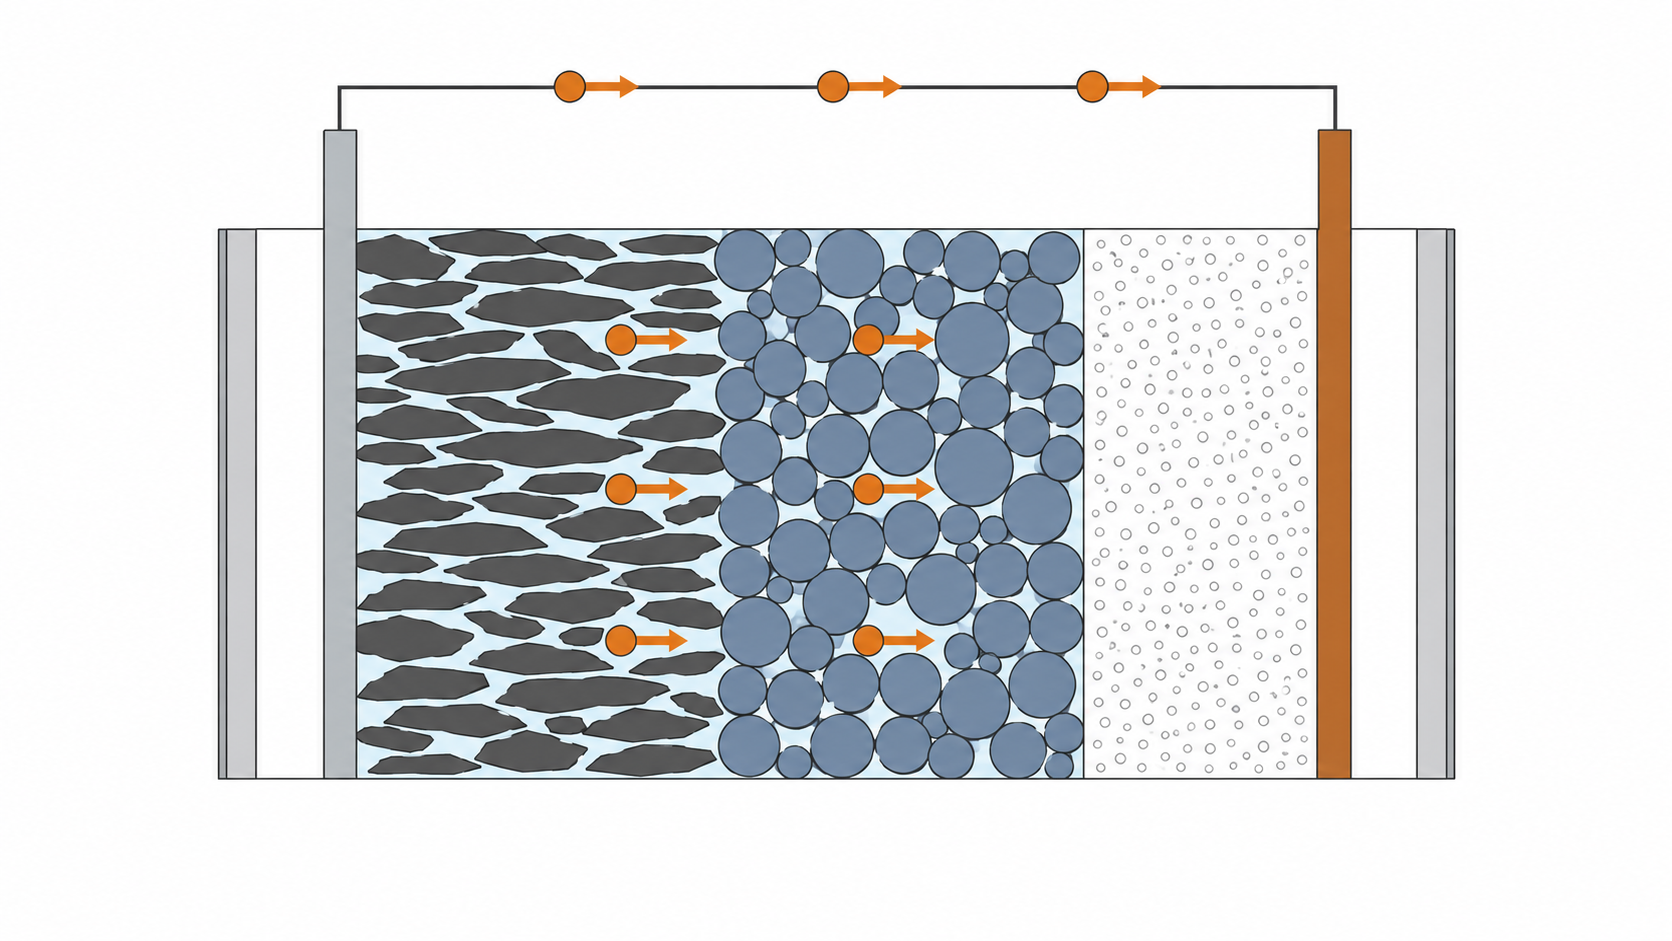
\includegraphics[width=\linewidth]{figures/ch07/ch07-07-battery-errors.png}};
  \begin{scope}[x={(img.south east)}, y={(img.north west)},
    font=\sffamily\small]
    \node[font=\bfseries] at (0.50, 1-0.02) {充电（错误示例）};
    \node[font=\scriptsize] at (0.20, 1-0.90) {铝箔};
    \node[font=\scriptsize, align=center] at (0.315, 1-0.90) {负极\\（石墨）};
    \node[font=\scriptsize, align=center] at (0.525, 1-0.90) {正极\\（如 LiCoO$_2$）};
    \node[font=\scriptsize] at (0.69, 1-0.90) {隔膜};
    \node[font=\scriptsize] at (0.76, 1-0.94) {铜箔};
    \node[font=\scriptsize, rotate=90, anchor=south] at (0.15, 1-0.20) {外壳};
    \node[font=\scriptsize] at (0.20, 1-0.11) {负极极耳};
    \node[font=\scriptsize] at (0.76, 1-0.11) {正极极耳};
    \node[font=\scriptsize\bfseries, text=white, fill=ch07err, circle, inner sep=1.5pt] at (0.20, 1-0.22) {❶};
    \node[font=\scriptsize\bfseries, text=white, fill=ch07err, circle, inner sep=1.5pt] at (0.76, 1-0.22) {❶};
    \node[font=\scriptsize\bfseries, text=white, fill=ch07err, circle, inner sep=1.5pt] at (0.42, 1-0.22) {❷};
    \node[font=\scriptsize\bfseries, text=white, fill=ch07err, circle, inner sep=1.5pt] at (0.40, 1-0.55) {❸};
    \node[font=\scriptsize\bfseries, text=white, fill=ch07err, circle, inner sep=1.5pt] at (0.50, 1-0.08) {❹};
    \node[font=\scriptsize, text=BookInk!80, anchor=north] at (0.50, 1-0.96)
      {❶–❹ 对应表~7-3 的 S2、S1、S4、S7};
  \end{scope}
\end{tikzpicture}

\caption{一张有意构造的错误电池结构示意（图像模型按“错误”要求生成）。❶ 铜、铝集流体对调；❷ 隔膜不在两电极之间，两极直接接触（实际电池中意味着内短路）；❸ 标为充电，但 $\text{Li}^+$ 从负极流向正极；❹ $\text{Li}^+$ 被画进外电路。对照正确画法见图~\ref{fig:ch07-08}。}\label{fig:ch07-07}
\end{figure}

为什么正确画法（图~\ref{fig:ch07-08}）不让图像模型画箭头？因为箭头方向是本图的核心科学内容，在充电与放电两种状态下恰好相反；若分两次生成，层厚与颗粒排布会发生随机漂移，读者会误以为充放电改变了宏观层结构。因此我们采用“结构底图只画一次，两套过程箭头全部在 TikZ 中叠加”的方案。任务书如下：

\begin{Prompt}
【用途与读者】论文引言/组会用结构示意图，单栏宽约 85 mm 两面板竖排，或双栏 174 mm 两面板并排；
读者为材料与化学方向的同行与研究生。
【目标】让读者看清一个锂离子电池单元的层序与材料对应，并区分充电与放电时 Li+ 和电子各自的路径与方向。
【材料】教科书级共识（Goodenough & Park 2013 等）；不含实验数据。
【对象】外壳铝塑膜（两侧）、铜集流体与负极极耳、石墨负极涂层、多孔隔膜、
正极涂层（层状氧化物，如 LiCoO2）、铝集流体与正极极耳、电解液（浸润孔隙）。每层只出现一次。
【关系/过程】结构底图中不画任何过程。叠加层：
(a) 充电：Li+ 正极 → 隔膜 → 负极；电子 正极极耳 → 充电器 → 负极极耳。
(b) 放电：Li+ 负极 → 隔膜 → 正极；电子 负极极耳 → 负载 → 正极极耳。
Li+ 只在电池内部；电子只在外电路。
【布局】横向截面，各层为竖直条带自左至右排列；极耳从集流体顶端伸出；
顶部留白给外电路，底部留白给图例。
【视觉】白底扁平二维；铜色、银灰、炭黑、灰蓝四种材料色加极浅蓝电解液；无渐变阴影 3D。
【限制】底图无任何文字、符号、离子、箭头、导线；不画 SEI、黏结剂、导电剂、分子结构；厚度不按比例。
【图例】Li+ 迁移（橙色实线实心头）、电子流（深灰虚线）、电解液（浅蓝）。
【验收】S1–S8 全部正确；两面板底图为同一文件；图注说明简化与命名约定。
\end{Prompt}

按上述任务书生成结构底图时，我们将同一提示词生成了三次：第一次在外壳膜与集流体之间多画了两条浅蓝竖带，看起来像独立的液体层（违反 S3）；第三次隔膜圆孔发白且正极颗粒过稀；第二次生成的结果严格呈现“外壳膜—铜集流体—片状石墨负极—中央多孔隔膜—球形正极—铝集流体—外壳膜”的层序，且无任何离子、导线或文字（放大检查仅见隔膜个别孔隙的浅蓝填充略有不均）。排版时，我们把这一张底图并排调用两次，在 TikZ 中分别叠加上方外电路（充电器或负载）、电子流虚线（$\text{e}^-$）与内部穿过隔膜的 $\text{Li}^+$ 橙色实线箭头（图~\ref{fig:ch07-08}）。顺带说明：把位图转成 PPTX 或 SVG 只能分离文字与背景，不会把颗粒或隔膜变成带科研语义的矢量对象，因此方向箭头仍应在 TikZ 或排版软件中绘制。

\begin{figure}[htbp]\centering
% FIG ch07-08 charge/discharge overlay (Chinese) — shared structural base, twice
\definecolor{ch07Li}{HTML}{D9822B}
\definecolor{ch07wire}{HTML}{3A3A3A}
\definecolor{ch07elec}{HTML}{3A3A3A}
\definecolor{ch07electrolyte}{HTML}{E3F0F8}
\makeatletter
\@ifundefined{chsevenpanelbase}{%
  \newcommand{\chsevenpanelbase}{figures/ch07/ch07-08-battery-base.png}
}{}
\@ifundefined{chsevendrawcircuit}{%
\newcommand{\chsevendrawcircuit}[1]{%
  \def\ChSevenWireY{1.10}%
  \def\ChSevenTabY{0.878}%
  \draw[ch07wire, line width=0.8pt] (0.194, \ChSevenTabY) -- (0.194, \ChSevenWireY);
  \draw[ch07wire, line width=0.8pt] (0.805, \ChSevenTabY) -- (0.805, \ChSevenWireY);
  \draw[ch07wire, line width=0.8pt] (0.194, \ChSevenWireY) -- (0.805, \ChSevenWireY);
  \node[draw=ch07wire, line width=0.6pt, rounded corners=1.5pt, fill=white,
    font=\sffamily\scriptsize, inner sep=1.6pt]
    at (0.50, \ChSevenWireY) {#1};
  \foreach \chyy in {0.38, 0.52, 0.66} {%
    \draw[-{Stealth[length=2mm]}, ch07Li, line width=0.9pt]
      (0.68, 1-\chyy) -- (0.32, 1-\chyy);
  }%
  \node[font=\sffamily\scriptsize, text=ch07Li, fill=white, inner sep=0.7pt]
    at (0.50, 1-0.30) {Li\textsuperscript{+}};
  \draw[ch07elec, line width=0.7pt, dashed, -{Stealth[length=1.5mm]}]
    (0.76, \ChSevenWireY) -- (0.62, \ChSevenWireY);
  \draw[ch07elec, line width=0.7pt, dashed, -{Stealth[length=1.5mm]}]
    (0.38, \ChSevenWireY) -- (0.24, \ChSevenWireY);
}
}{}
\@ifundefined{chsevendrawcircuitb}{%
\newcommand{\chsevendrawcircuitb}[1]{%
  \def\ChSevenWireY{1.10}%
  \def\ChSevenTabY{0.878}%
  \draw[ch07wire, line width=0.8pt] (0.194, \ChSevenTabY) -- (0.194, \ChSevenWireY);
  \draw[ch07wire, line width=0.8pt] (0.805, \ChSevenTabY) -- (0.805, \ChSevenWireY);
  \draw[ch07wire, line width=0.8pt] (0.194, \ChSevenWireY) -- (0.805, \ChSevenWireY);
  \node[draw=ch07wire, line width=0.6pt, rounded corners=1.5pt, fill=white,
    font=\sffamily\scriptsize, inner sep=1.6pt]
    at (0.50, \ChSevenWireY) {#1};
  \foreach \chyy in {0.38, 0.52, 0.66} {%
    \draw[-{Stealth[length=2mm]}, ch07Li, line width=0.9pt]
      (0.32, 1-\chyy) -- (0.68, 1-\chyy);
  }%
  \node[font=\sffamily\scriptsize, text=ch07Li, fill=white, inner sep=0.7pt]
    at (0.50, 1-0.30) {Li\textsuperscript{+}};
  \draw[ch07elec, line width=0.7pt, dashed, -{Stealth[length=1.5mm]}]
    (0.24, \ChSevenWireY) -- (0.38, \ChSevenWireY);
  \draw[ch07elec, line width=0.7pt, dashed, -{Stealth[length=1.5mm]}]
    (0.62, \ChSevenWireY) -- (0.76, \ChSevenWireY);
}
}{}
\makeatother
\begin{tikzpicture}
  \node[anchor=south west, inner sep=0] (imgA) at (0,0)
    {\includegraphics[width=0.49\linewidth]{\chsevenpanelbase}};
  \node[anchor=south west, inner sep=0] (imgB) at (0.51\linewidth,0)
    {\includegraphics[width=0.49\linewidth]{\chsevenpanelbase}};
  \begin{scope}[shift={(imgA.south west)},
    x={($(imgA.south east)-(imgA.south west)$)},
    y={($(imgA.north west)-(imgA.south west)$)},
    font=\sffamily\small]
    \node[anchor=south west, font=\sffamily\small] at (0.00, 1.20) {\textbf{(a)} 充电};
    \node[font=\sffamily\scriptsize, anchor=north west] at (0.25, 1.045) {负极极耳};
    \node[font=\sffamily\scriptsize, anchor=north east] at (0.75, 1.045) {正极极耳};
    \chsevendrawcircuit{充电器}
  \end{scope}
  \begin{scope}[shift={(imgB.south west)},
    x={($(imgB.south east)-(imgB.south west)$)},
    y={($(imgB.north west)-(imgB.south west)$)},
    font=\sffamily\small]
    \node[anchor=south west, font=\sffamily\small] at (0.00, 1.20) {\textbf{(b)} 放电};
    \chsevendrawcircuitb{负载}
  \end{scope}
  \begin{scope}[shift={(imgA.south west)},
    x={($(imgA.south east)-(imgA.south west)$)},
    y={($(imgA.north west)-(imgA.south west)$)},
    font=\sffamily\scriptsize]
    \node[align=center, anchor=north] at (0.323, 0.19) {负极\\（石墨）};
    \node[anchor=north] at (0.50, 0.19) {隔膜};
    \node[align=center, anchor=north] at (0.678, 0.19) {正极\\（LiCoO\textsubscript{2}）};
    \draw[BookInk!45, thin] (0.193, 0.19) -- (0.193, -0.02);
    \node[align=center, anchor=north] at (0.193, -0.02) {铜\\集流体};
    \draw[BookInk!45, thin] (0.806, 0.19) -- (0.806, -0.02);
    \node[align=center, anchor=north] at (0.806, -0.02) {铝\\集流体};
  \end{scope}
  \node[anchor=north, font=\sffamily\scriptsize, align=center] at (0.5\linewidth, -0.13\linewidth) {%
    \begin{tabular}{@{}c@{\qquad}c@{}}
      \tikz{\draw[-{Stealth[length=1.5mm]}, ch07Li, line width=0.7pt] (0,0) -- (0.2,0);} Li\textsuperscript{+} 迁移（电解液中） &
      \tikz{\draw[ch07elec, line width=0.6pt, dashed, -{Stealth[length=1.2mm]}] (0,0) -- (0.2,0);} 电子流（外电路） \\[0.4em]
      \multicolumn{2}{c}{\tikz{\fill[ch07electrolyte] (0,0) rectangle (0.08,0.06);} 电解液（填充孔隙）} \\[0.35em]
      \multicolumn{2}{c}{两侧浅灰竖条为外壳}
    \end{tabular}};
\end{tikzpicture}

\caption{锂离子软包电池一个重复单元的截面示意。两面板使用同一张结构底图（图像模型生成，不含文字和箭头），箭头、外电路与标签由 LaTeX 叠加。（a）充电：$\text{Li}^+$ 从正极脱出，经电解液穿过隔膜嵌入石墨负极，电子经外电路由正极流向负极。（b）放电：方向相反，电子经负载由负极流向正极。负极使用铜集流体，正极使用铝集流体；电解液浸润电极与隔膜的孔隙。各层厚度不按比例（隔膜被加宽），只画一个单元（实际软包由多层双面涂布极片叠片或卷绕），省略 SEI、黏结剂、导电剂与封装细节；“负极/正极”即按放电约定所称的阳极/阴极。}\label{fig:ch07-08}
\end{figure}

\section{AI 能做什么、不能做什么、作者要核对什么}

表~\ref{tab:ch07-02} 汇总了机制图与结构示意图各环节中 AI（含 SciDraw AI）的能力边界与作者必须核对的事项。

\begin{table}[htbp]\centering\footnotesize
\caption{机制图与结构示意图制作中 AI 能做、不能做与作者核对事项对照表。}\label{tab:ch07-02}
\begin{tabularx}{\linewidth}{lYYY}
\toprule
\textbf{环节} & \textbf{AI（含 SciDraw AI）能做} & \textbf{AI 不能做} & \textbf{作者要核对} \\
\midrule
整理关系 & 把作者写好的关系表改写成提示词段落；在科研绘图向导中按“机制图与流程图”路线组织任务书 & 判断某条关系是否已确立、是否有争议；自动阅读整篇论文并找出正确机制 & 每条关系都有文献依据；确立 / 简化 / 假设的标注；“不画的内容”清单 \\
草图与布局 & 草图模式把草图与文字一起作为生成输入，给出大致遵循布局的候选图 & 保证布局硬性保持或对象锁定；同一提示词两次给出相同排布 & 分区、阅读路径、对象数量；与草图的偏差 \\
生成底图 & 机制图生成或提示词绘图按任务书产出扁平风格的无字候选图；批量候选 & 保证不多画、不漏画、不出现伪文字；保证色值和线宽精确 & 用核验表逐条核对 R1–R13 或 S1–S8；放大检查伪字符 \\
修改 & 选择历史图并输入修改指令，进行连续迭代 & 只改指定之处而不影响其他部分 & 每次修改后全表复核，记录意外变化 \\
线型与颜色 & 按提示词中定义的线型与色板绘制；图片检查给出灰度、色觉风险、分辨率等技术报告 & 自行决定线型的科学含义；技术检查不代表科学审核 & 图例与线型一一对应；颜色只承担角色；灰度可辨 \\
标签与方向 & 无（本章做法：标签与关键箭头不交给图像模型） & 可靠拼写分子名、上下标；在不同状态下保持结构不变而只翻转方向 & 标签逐字从清单复制；箭头方向与过程状态一致 \\
图注 & 图注辅助根据图片起草图注草稿 & 知道作者省略了什么、依据哪篇文献；补写样本量或统计（本类图本就不应出现） & 每句对应关系表；简化与省略写全；中英文各自通顺 \\
交付 & 组图工具排版与导出（第九章） & 图像转 PPTX/SVG 不会把底图变成带科研语义的可编辑对象 & 终稿文字为排版文字；底图分辨率足够；同行复核 \\
\bottomrule
\end{tabularx}
\end{table}

\section{本章检查清单}

\begin{itemize}
\item 先有关系表（起点、终点、关系类型、位置、证据状态），再写提示词；列出“不画的内容”。
\item 每个对象出现次数明确；允许重复的对象（如 GLUT4 的储存态与膜上态）在任务书中写明。
\item 空间分区（胞外/膜/胞质，或结构图的层序）写进任务书，并在图中可辨。
\item 每种关系类型只用一种线型；图例定义全部线型；假设关系与确立关系可区分。
\item 没有“捷径箭头”：间接作用（如“抑制的抑制”）保留中间环节。
\item 颜色只编码角色，色相不超过 3 个加灰色；灰度下关系仍可读。
\item 底图放大检查无伪文字、无多余对象；所有标签由排版生成，逐字从清单复制。
\item 结构图：层序、材料对应、过程方向、状态（如充电/放电）逐项核对；结构只画一次，状态用叠加层区分。
\item 每次 AI 修改后完整复核，而不只看改动处；记录意外变化。
\item 图注写明简化、省略与依据；不写任何数据或统计。
\item 至少一位领域同行复核关系与结构。
\end{itemize}

\section{本章练习}

\begin{enumerate}
\item \textbf{拆捷径箭头（纸笔）。} 常见教学图写着“$\text{Akt} \rightarrow \text{GLUT4 translocation}$”。（a）写出省略的中间环节，并为每一环指定图~\ref{fig:ch07-01} 中的线型；（b）解释为什么 Akt 与 AS160 之间画抑制线，而整条通路的净效应是促进转位；（c）写成三行关系表（起点、终点、关系、线型、依据），注明你查阅的综述及其具体部分。

\item \textbf{SciDraw AI 实操：同一机制，两种输入。} 选一条你领域中教科书已确立、不超过 8 个对象的机制。（a）在科研绘图向导选择“机制图与流程图”路线，按十个填写项写任务书（必须含空间分区与线型定义），下载副本；（b）先在机制图生成中只输入一句话，按本章核验表记录至少 5 处问题；（c）再粘贴完整任务书生成无字底图，比较两份核验表；（d）选一张历史图输入一条修改指令，记录至少一处“意外变化”。提交两张图、两份核验表、一条修改指令和修改记录。

\item \textbf{结构图找错与改正。} 以质子交换膜燃料电池（PEMFC）单电池截面为对象（或你领域的另一种层状器件）：（a）写出自左至右的层序与每层材料，以及工作时 $\text{H}^+$、电子、$\text{H}_2/\text{O}_2/\text{H}_2\text{O}$ 各自的路径和方向，并给出依据文献；（b）设计一张故意含 3 处错误的提示词，再写一份正确的结构底图提示词（不含箭头与文字）；（c）用 TikZ 在正确底图上叠加过程箭头与标签，并用灰度打印检查线型可辨。
\end{enumerate}

\section*{参考文献}

\begin{itemize}
\item Armand M, Tarascon JM. Building better batteries. \emph{Nature}. 2008;451(7179):652--657. doi:10.1038/451652a
\item Arora P, Zhang Z. Battery separators. \emph{Chem Rev}. 2004;104(10):4419--4462. doi:10.1021/cr020738u
\item ColorBrewer 2.0: Color advice for cartography and scientific visualization. \url{https://colorbrewer2.org/}
\item Goodenough JB, Park KS. The Li-ion rechargeable battery: a perspective. \emph{J Am Chem Soc}. 2013;135(4):1167--1176. doi:10.1021/ja3091438
\item Klip A, McGraw TE, James DE. Thirty sweet years of GLUT4. \emph{J Biol Chem}. 2019;294(30):11369--11381. doi:10.1074/jbc.REV119.008351
\item Le Nov\`ere N, Hucka M, Mi H, Moodie S, Schreiber F, Sorokin A, et al. The Systems Biology Graphical Notation. \emph{Nat Biotechnol}. 2009;27(8):735--741. doi:10.1038/nbt.1558
\item Leto D, Saltiel AR. Regulation of glucose transport by insulin: traffic control of GLUT4. \emph{Nat Rev Mol Cell Biol}. 2012;13(6):383--396. doi:10.1038/nrm3351
\item Nitta N, Wu F, Lee JT, Yushin G. Li-ion battery materials: present and future. \emph{Mater Today}. 2015;18(5):252--264. \path{doi:10.1016/j.mattod.2014.10.040}
\item Rougier NP, Droettboom M, Bourne PE. Ten simple rules for better figures. \emph{PLoS Comput Biol}. 2014;10(9):e1003833. \path{doi:10.1371/journal.pcbi.1003833}
\item Saltiel AR, Kahn CR. Insulin signalling and the regulation of glucose and lipid metabolism. \emph{Nature}. 2001;414(6865):799--806. doi:10.1038/414799a
\item Sano H, Kane S, Sano E, M\^{\i}inea CP, Asara JM, Lane WS, Garner CW, Lienhard GE. Insulin-stimulated phosphorylation of a Rab GTPase-activating protein regulates GLUT4 translocation. \emph{J Biol Chem}. 2003;278(17):14599--14602. doi:10.1074/jbc.C300063200
\item Sarbassov DD, Guertin DA, Ali SM, Sabatini DM. Phosphorylation and regulation of Akt/PKB by the Rictor-mTOR complex. \emph{Science}. 2005;307(5712):1098--1101. doi:10.1126/science.1106148
\item Systems Biology Graphical Notation (SBGN) official website. \url{https://sbgn.github.io/}
\item Tarascon JM, Armand M. Issues and challenges facing rechargeable lithium batteries. \emph{Nature}. 2001;414(6861):359--367. doi:10.1038/35104644
\item Wong B. Points of view: Color blindness. \emph{Nat Methods}. 2011;8(6):441. doi:10.1038/nmeth.1618
\item Xu K. Nonaqueous liquid electrolytes for lithium-based rechargeable batteries. \emph{Chem Rev}. 2004;104(10):4303--4418. doi:10.1021/cr030203g
\end{itemize}

\chapter{实验图像的科学呈现}

细胞生物学专业的研究生小苏正在整理一篇关于小分子化合物高内涵表型筛选的论文。为了在补充材料中展示对照孔（DMSO 处理）人骨肉瘤细胞（U2OS）的细胞核与线粒体荧光染色质量，她从显微镜工作站拷出几张图，顺手拖进幻灯片软件里把偏暗的线粒体面板“调亮一点、拉高对比度”，截屏保存成图片后，又把截图上传到一个生成式图像工具，输入指令“去噪、变清晰、提升分辨率”。

组会上，导师没有评价画面好不好看，只问了三个问题：第一，未经改动的 16 位原始文件保存在哪里？第二，细胞核与线粒体通道各自映射的是哪一段原始灰度值，对照视野之间用的是不是同一套显示范围？第三，右下角那根标着“$20\ \mu\text{m}$”的比例尺，是根据哪个物镜和相机像素尺寸算出来的？小苏一个也答不上来：截图早已把 16 位数值压成了 8 位 RGB，幻灯片滑块没有留下任何数值记录，比例尺则是照着另一篇论文的图估算着画上去的。

实验图像与本书第 6 章的流程图、第 7 章的机制示意图有着本质区别：\textbf{实验图像是测量，不是插画。}在显微镜照片、扫描电子显微镜（SEM）图像、蛋白印迹（Western blot）或组织病理切片中，每一个像素的数值都对应探测器在特定空间位置接收到的光子数或电子数。面对这类证据图像，AI 工具只承担三项辅助工作：协助整理呈现计划、起草确定性的图像读取与排版脚本、对导出图做格式与色觉等技术检查；\textbf{AI 绝不触碰证据图像的任何像素值。}本章围绕多通道荧光显微图与植物叶片扫描电镜图两类公开原始图像，拆解从原始文件管理、显示映射、伪彩色选择、裁剪与比例尺校准，到期刊图像诚信规则与完整交付记录的全流程。

\section{原始图像是证据：数据、显示与导出}

在数字成像系统中，\textbf{原始数据、显示设置与导出图}是三件完全不同的事物。混淆这三者，是绝大多数实验图像失真与合规问题的起点。

当科研级相机（如 sCMOS 或 CCD）采集一幅荧光显微图像时，光电探测器将每个像素位置收集到的光子转化为电荷，再由模数转换器（ADC）量化为整数灰度值，通常按单通道 12 位（数值范围 $0\text{--}4095$）、14 位（$0\text{--}16383$）或 16 位（$0\text{--}65535$）保存在未压缩的 TIFF 或仪器原生格式（如 OME-TIFF、ND2、CZI、LIF）中。这个二维整数矩阵才是测量数据。

然而，普通的电脑显示器、网页和文档阅读器每个颜色通道只能显示 8 位灰度（$0\text{--}255$）。要把 16 位文件里的原始数值呈现在屏幕上，看图软件必须执行一步\textbf{显示映射（display mapping）}：选定一个下限值（黑点，$v_{\min}$）和一个上限值（白点，$v_{\max}$），把小于或等于 $v_{\min}$ 的像素显示为纯黑（$0$），把大于或等于 $v_{\max}$ 的像素显示为纯白（$255$），并把中间的数值按比例映射到 $0\text{--}255$ 之间。在线性映射下，任意像素原始数值 $I$ 对应的 8 位显示灰度 $I_{\text{disp}}$ 为：
\[
I_{\text{disp}} = \operatorname{clip}\!\left(\frac{I - v_{\min}}{v_{\max} - v_{\min}},\, 0,\, 1\right) \times 255
\]
只要不覆盖原始文件，改变黑点和白点只是换了一副观察数据的“窗口”，底层 TIFF 文件里的测量值并未改变；可一旦在软件里点击“另存为 8 位 JPEG/PNG”或直接截图，映射范围之外的数值就会被永久截断，12 位或 16 位的精细灰度级也会被不可逆地压缩为 256 个灰阶。

我们用 Broad 研究所公开生物图像基准库 BBBC022v1（Gustafsdottir 等，2013；Ljosa 等，2012；权利人 Anne Carpenter 声明按 CC0 1.0 献入公有领域）中的真实原始图像来演示这一区别。本章主材料取自该数据集第 20585 号微孔板的 A13 孔（DMSO 溶剂对照，元数据标记为 \texttt{mock}）第 1 视野（\texttt{s1}）与第 2 视野（\texttt{s2}），包含两个单通道文件：通道 \texttt{w1} 为 Hoechst 33342 染色的细胞核，通道 \texttt{w5} 为 MitoTracker Deep Red 染色的线粒体。每个文件均为 $696 \times 520$ 像素的 16 位灰度 TIFF，但采集相机的有效位深为 12 位（理论上限 $4095$）。

读取第 1 视野细胞核通道（\texttt{w1}）的原始矩阵可知，全图 $361,920$ 个像素的数值分布在 $121\text{--}1655$ 之间，均值为 $238.4$，第 $0.1\%$ 与第 $99.9\%$ 分位数分别为 $132$ 与 $1236$，没有任何像素达到相机上限 $4095$。图~\ref{fig:ch08-01} 展示了这一份 16 位原始矩阵在三种线性显示映射下的画面及对应的原始数值直方图。

\begin{figure}[htbp]\centering
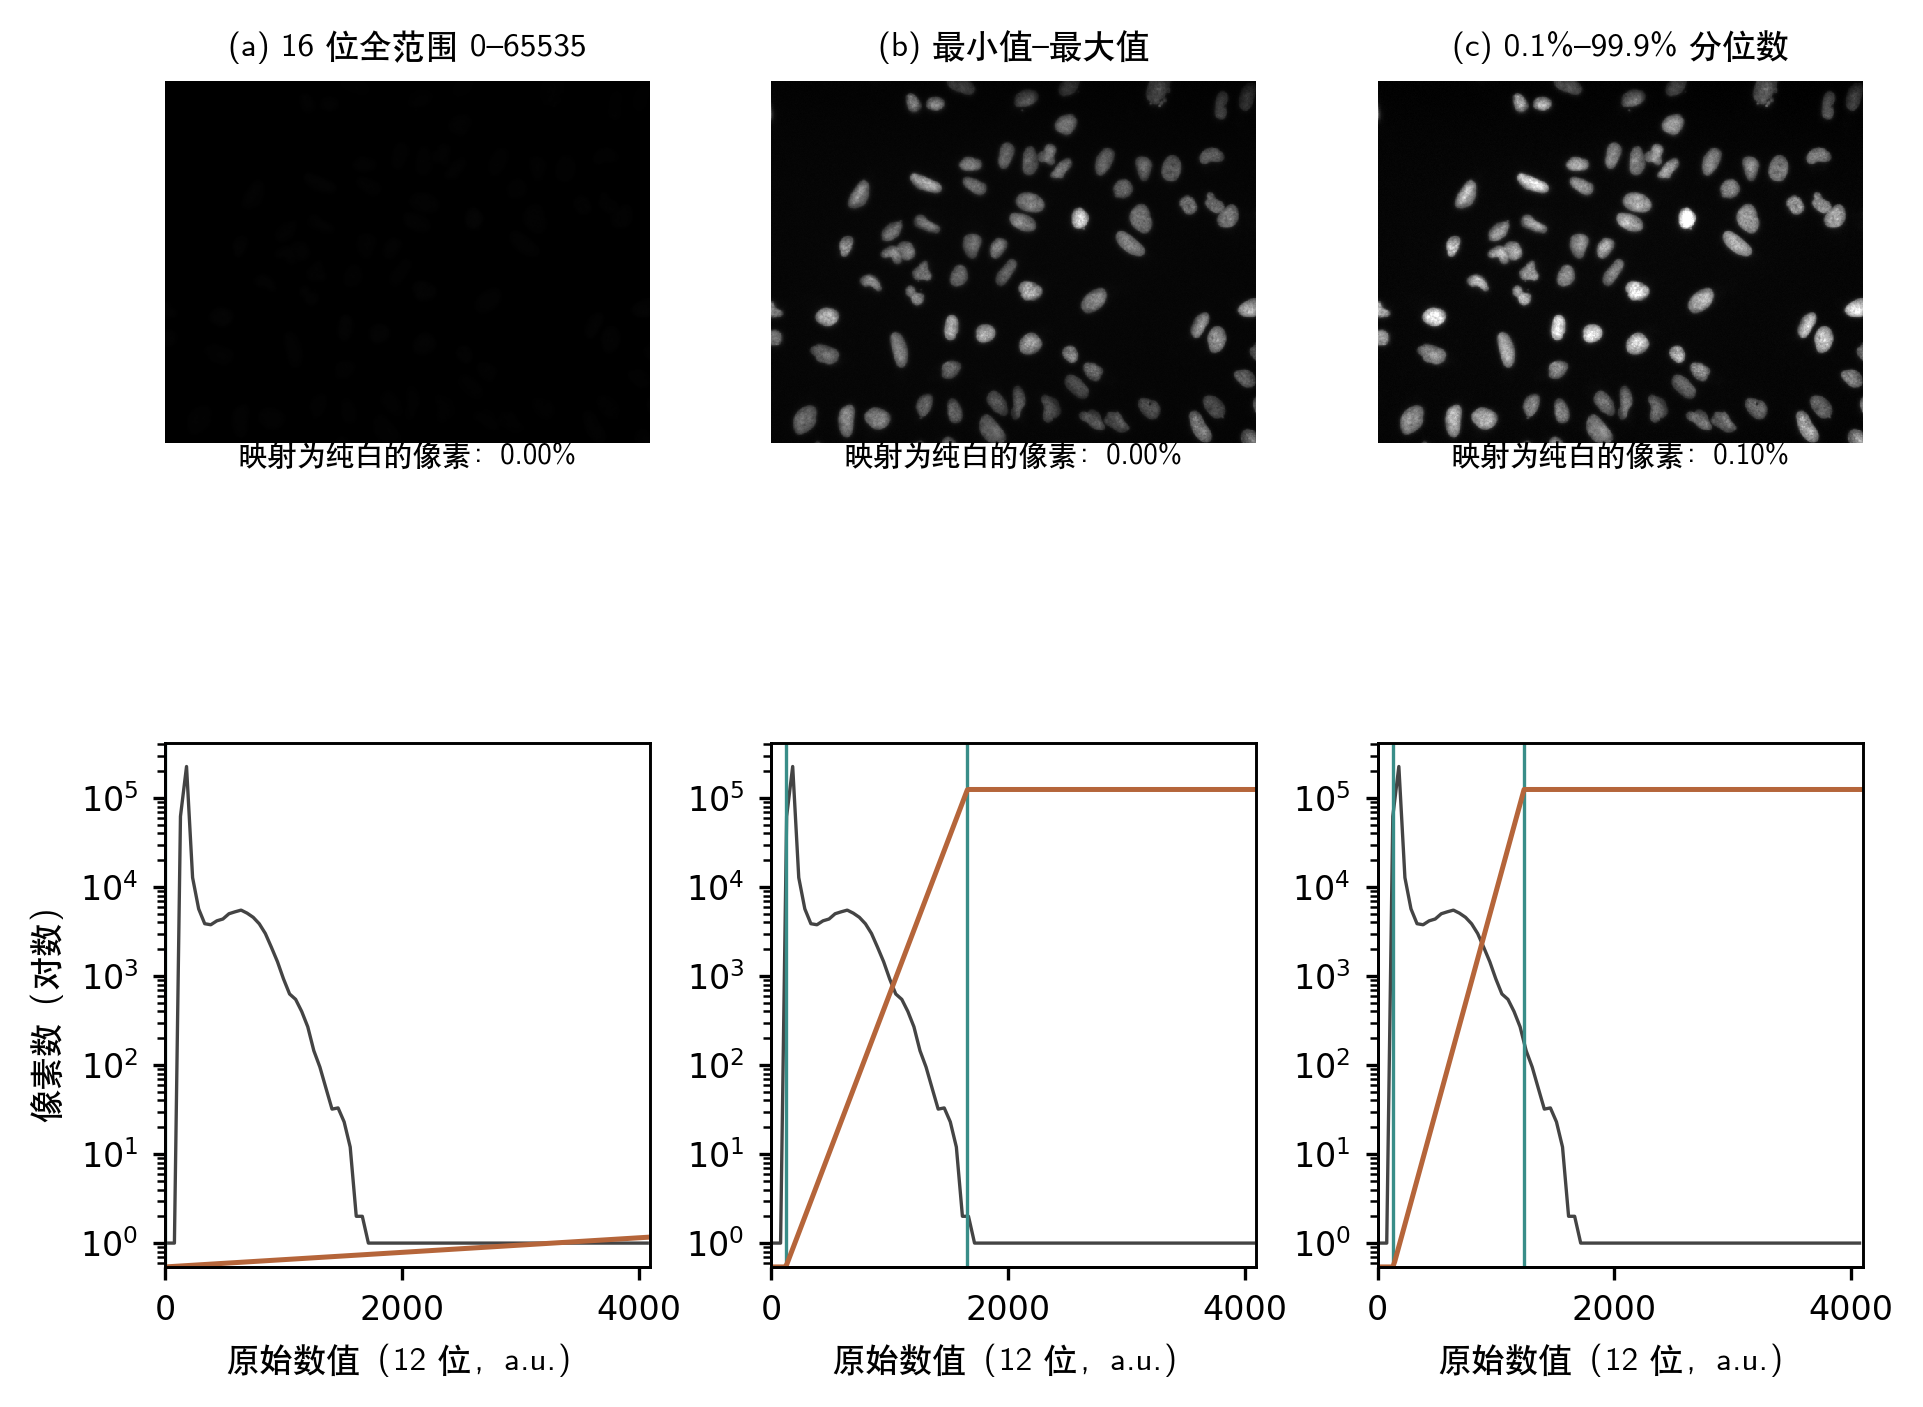
\includegraphics[width=0.88\linewidth]{figures/ch08/ch08-01-raw-display-mapping-zh.png}
\caption{同一幅 16 位荧光原图（BBBC022，Hoechst 通道）的三种线性显示。原始像素值在三列中完全相同，改变的只是显示映射：(a) 按 16 位全范围；(b) 按图像最小值至最大值；(c) 按 $0.1\%$ 与 $99.9\%$ 分位数，图中注明被映射为纯白的像素比例。下排为原始数值直方图与映射线。图像：BBBC022v1，CC0。}\label{fig:ch08-01}
\end{figure}

对照图~\ref{fig:ch08-01} 的三列，可以清楚看到显示映射如何改变画面外观：
\begin{itemize}
\item \textbf{列 (a)（按 16 位容器全范围 $0\text{--}65535$ 线性映射）：}许多操作系统的自带看图器在打开 16 位 TIFF 时，默认把 $0$ 当作黑点、$65535$ 当作白点。由于 12 位相机的读数不会超过 $4095$，且该视野细胞核的最高值仅为 $1655$，最亮的像素在映射后也只有 $1655 / 65535 \times 255 \approx 6.4$ 的灰度值。结果上排左图看起来几乎全黑（映射为纯白的像素为 $0.00\%$），下排直方图中的棕色映射直线紧贴在横轴底部。不少初学者看到这团漆黑，误以为拍摄失败，或者急忙用修图软件“拉亮并保存”，无意间毁掉了原件。
\item \textbf{列 (b)（按图像最小值至最大值 $121\text{--}1655$ 线性映射）：}将黑点设为全图最小值 $121$、白点设为最大值 $1655$（下排中图两条青色竖线所夹区间），映射直线斜率抬升，视野内约 60 颗细胞核全部显现，被映射为纯白的像素依然是 $0.00\%$。但画面右上偏中位置有一颗高度浓缩的极亮细胞核，它把全图最大值推高到了 $1655$，导致其余绝大多数处于间期的细胞核显得偏暗。
\item \textbf{列 (c)（按 $0.1\%\text{--}99.9\%$ 分位数 $132\text{--}1236$ 线性映射）：}将黑点设在第 $0.1\%$ 分位数（$132$）、白点设在第 $99.9\%$ 分位数（$1236$），仅有最亮的 $0.10\%$ 像素（集中于那颗极亮细胞核内）被映射为纯白，而视野内大多数细胞核的染色质细节得以清晰呈现。
\end{itemize}

这里必须区分两种完全不同的“像素封顶”：一种是列 (c) 中在\textbf{显示阶段}将极少数高值像素映射为纯白（原始 TIFF 里的 $1655$ 完好无损）；另一种则是\textbf{采集阶段}发生在相机传感器内部的物理饱和。检查同一视野的线粒体通道（\texttt{w5}）原始矩阵可知，其像素值范围为 $185\text{--}4095$，均值为 $373.2$，其中有 \textbf{12 个像素等于 12 位 ADC 的上限 $4095$}。这 12 个像素在曝光结束时就已经溢出，后期任何算法都无法恢复其真实荧光强度。对于采集饱和，唯一的诚实做法是在原图目录与图注中如实报告饱和像素数量，不做修补；若饱和面积较大影响定量，只能调低曝光重拍。

因此，实验图像管理的第一条原则是：\textbf{先复制再处理，原件设为只读。}图像从仪器导出后应立即存入只读目录，建立包含文件名、SHA-256 哈希、位深、尺寸、像素尺寸与采集信息的\textbf{原图目录}；后续所有显示映射与裁剪一律通过确定性脚本读取原件并将显示版另存为无损 PNG 或 TIFF，绝不用有损 JPEG 压缩图或屏幕截图充当源图。在这一步，通用 AI 对话助手可以协助编写读取原始目录、计算 SHA-256 与统计饱和像素的 Python 脚本；作者则必须亲自核实相机的有效位深（本例需按 $4095$ 而非 $65535$ 筛查饱和）以及物理像素尺寸的出处。

\section{对比度调整：线性、非线性与披露}

主流期刊（如 \textit{Journal of Cell Biology} 与 Nature Portfolio）对图像对比度调整划定了四条清晰边界：

\textbf{第一，整图线性调整是允许的，但不得让有效数据消失。}在线性窗口 $[v_{\min}, v_{\max}]$ 内，图中任意两个区域扣除黑点后的相对强度比值保持不变。相反，如果为了“让背景显得更干净”而把黑点拉高到背景信号之上，或者为了“让弱信号更显眼”而把白点压得过低，就会把大量真实信号截断成纯黑（$0$）或纯白（$255$），直接抹除结构细节。

\textbf{第二，伽马（$\gamma$）校正、对数变换或曲线等非线性调整会改变不同强度之间的相对比例，若确需使用必须在图注中明确披露。}伽马映射公式为：
\[
I_{\text{disp}} = \left[\operatorname{clip}\!\left(\frac{I - v_{\min}}{v_{\max} - v_{\min}},\, 0,\, 1\right)\right]^{\gamma} \times 255
\]
当 $\gamma < 1$（如 $\gamma = 0.5$）时，传递曲线向上凸起，暗部弱信号被大幅拉亮，亮部增长被压缩，原本相差数倍的强弱信号在画面上会变得接近。

图~\ref{fig:ch08-02} 用第 1 视野的线粒体通道（\texttt{w5}）对线性映射、$\gamma = 0.5$ 非线性映射以及白点过低的截断反例做了定量对比。我们在视野中固定选取两个 $15 \times 15$ 像素区域（ROI）：一处位于核周线粒体密集的亮区（坐标 $(340, 210)\text{--}(355, 225)$，图中青色短斜线），另一处位于胞质外缘信号较弱的暗区（坐标 $(120, 380)\text{--}(135, 395)$，图中黄色短斜线）。扣除黑点（$218$）后，亮区与暗区的原始平均强度比值为 $3.57$。

\begin{figure}[htbp]\centering
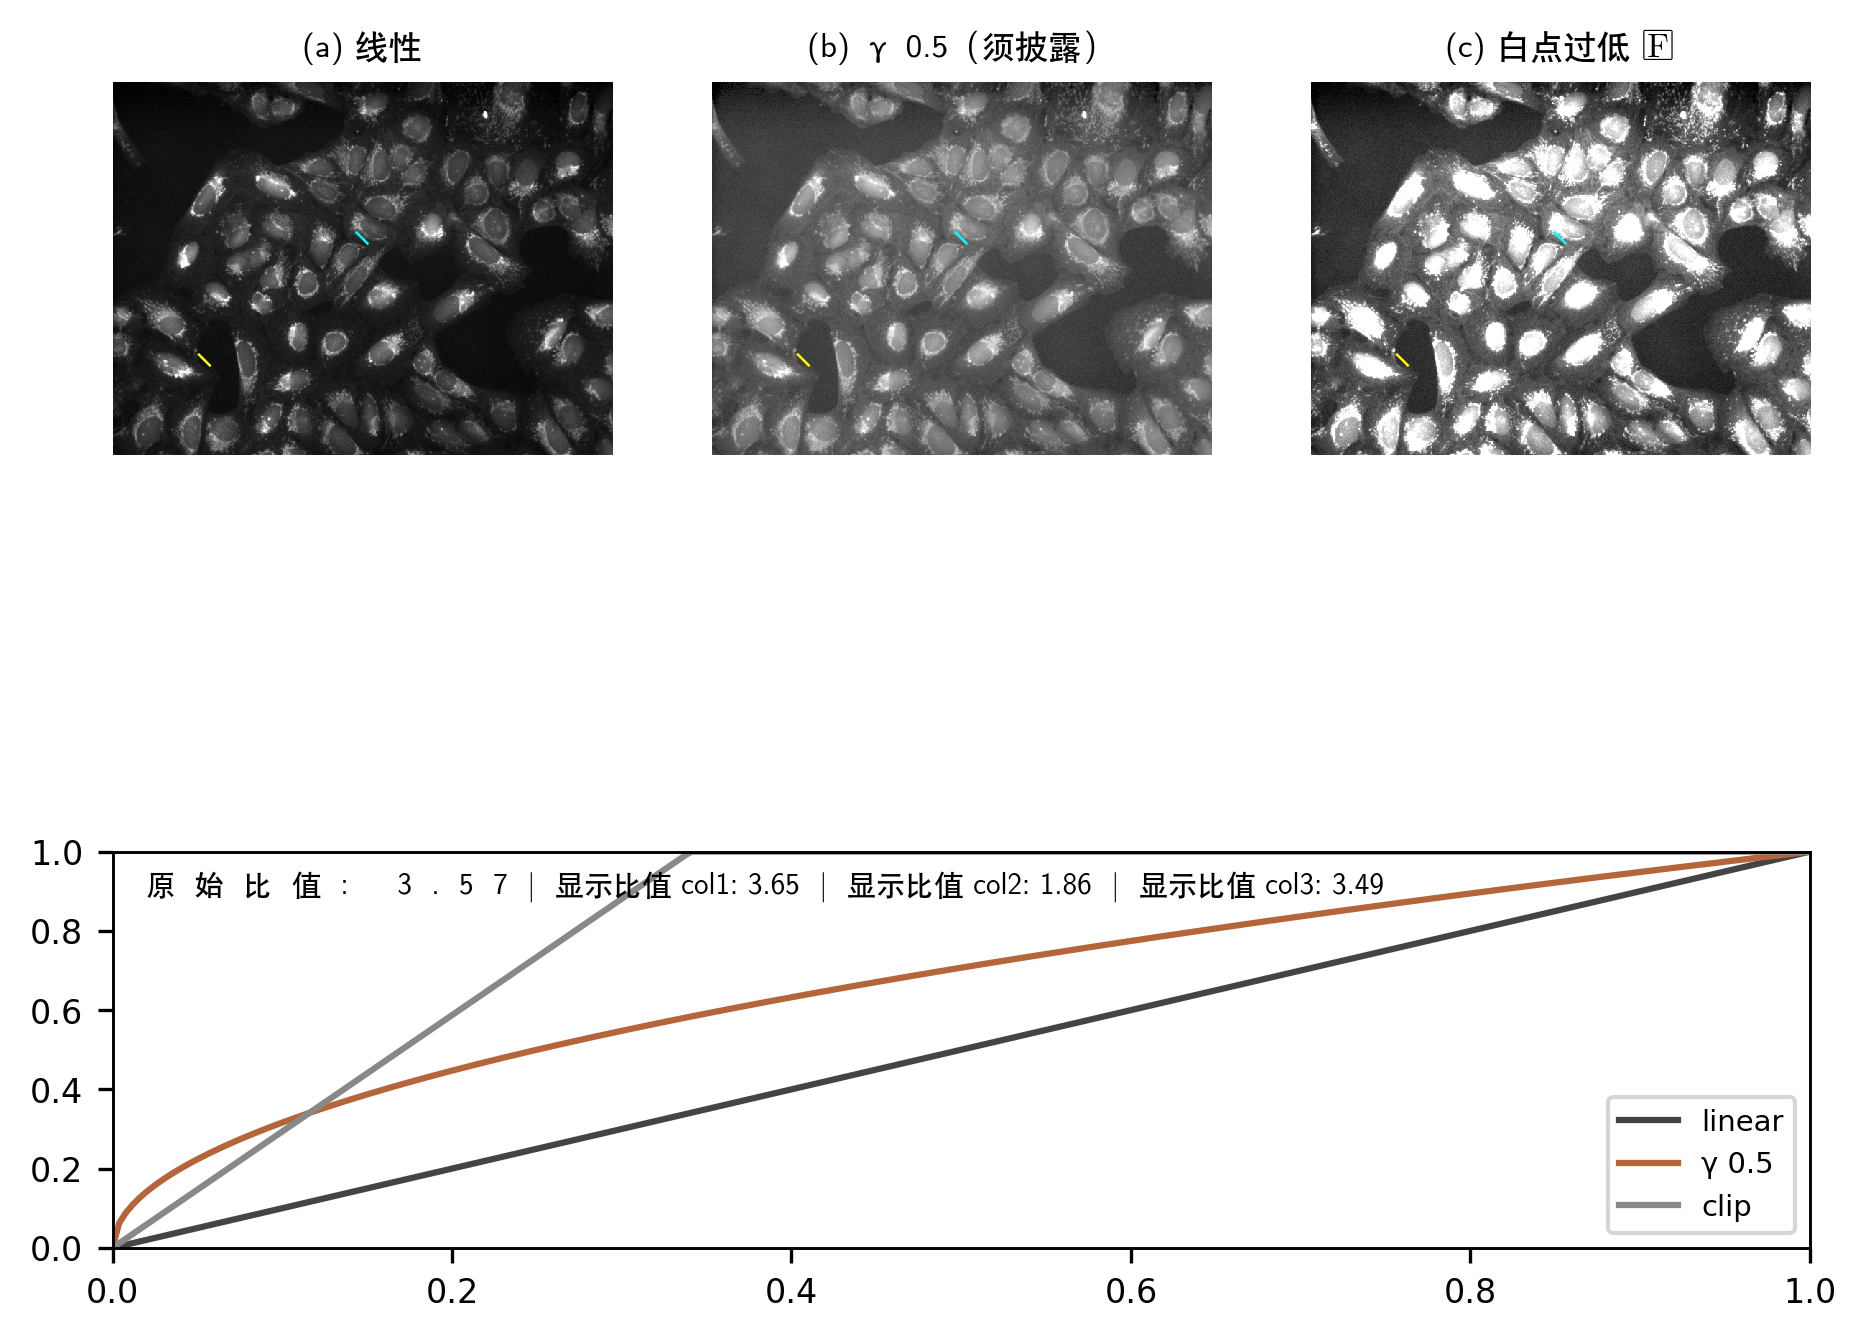
\includegraphics[width=0.88\linewidth]{figures/ch08/ch08-02-linear-vs-gamma-zh.png}
\caption{线性与非线性显示的区别。(a) 线性映射（$218\text{--}1140$）。(b) 同一图像施加 $\gamma = 0.5$，暗部信号变亮，亮暗区域的相对强度随之改变；这种调整必须在图注中披露。(c) 反例：白点过低导致大部分线粒体信号被截断为纯白，信息丢失。下方曲线为三种映射，并列出两个固定区域（青色与黄色短线）的原始强度比与显示灰度比。图像：BBBC022v1，CC0。}\label{fig:ch08-02}
\end{figure}

观察图~\ref{fig:ch08-02} 的三列画面与下方传递曲线：
\begin{enumerate}
\item \textbf{面板 (a)（线性映射 $218\text{--}1140$）：}核周线粒体簇与胞质远端细丝层次分明；亮、暗两处 ROI 的 8 位显示灰度比值为 $3.65$（\texttt{col1: 3.65}），与原始比值 $3.57$ 仅差 8 位整数舍入带来的微小偏差，真实保持了亮暗相对比例。
\item \textbf{面板 (b)（$\gamma = 0.5$，黑白点仍为 $218\text{--}1140$）：}下方棕色曲线向上拱起，胞质外周弱信号明显变亮，但两处 ROI 的显示灰度比值从 $3.57$ 降至 $1.86$（\texttt{col2: 1.86}），相对差距缩水近半。若不在图注中披露 $\gamma = 0.5$，读者就会误判信号的空间分布比例。
\item \textbf{面板 (c)（反例，白点设为第 $90\%$ 分位数 $532$）：}下方灰色折线在横轴约三分之一处即触顶封平，全图有 \textbf{$9.94\%$ 的像素被截断为纯白（$255$）}。尽管此时两个 ROI 的均值比读作 $3.49$（\texttt{col3: 3.49}，因为更陡的直线斜率在把亮区顶死在 $255$ 的同时，也把暗区同步拉高了），但画面上几乎所有核周线粒体都变成了刺眼的实心白斑，内部结构彻底丢失。
\end{enumerate}

\textbf{第三，严禁阈值化抹黑背景、局部涂抹或使用克隆修复工具。}无论是单独提亮某几颗细胞，还是用仿制图章（clone stamp）、修复画笔抹掉荧光杂质或背景斑点，都属于篡改原始测量数据（Rossner 与 Yamada，2004；Cromey，2010）。

\textbf{第四，同一组比较中的所有面板，必须使用完全相同的显示设置。}如果对每个面板分别点“自动对比度”，真实的处理效应会被抵消，而原本没有差异的对照视野却能被调出假差异。图~\ref{fig:ch08-03} 用同一对照孔（A13 孔，DMSO 对照）的两个相邻视野 \texttt{s1} 与 \texttt{s2}（线粒体通道）演示了这一后果：右侧柱状图计算了两幅 16 位原图的全幅平均强度，\texttt{s1} 为 $373.2\ \text{a.u.}$，\texttt{s2} 为 $366.3\ \text{a.u.}$，相差不到 $2\%$（注：每视野仅一个均值，此处仅用于核对原始量级，不是统计检验）。

\begin{figure}[htbp]\centering
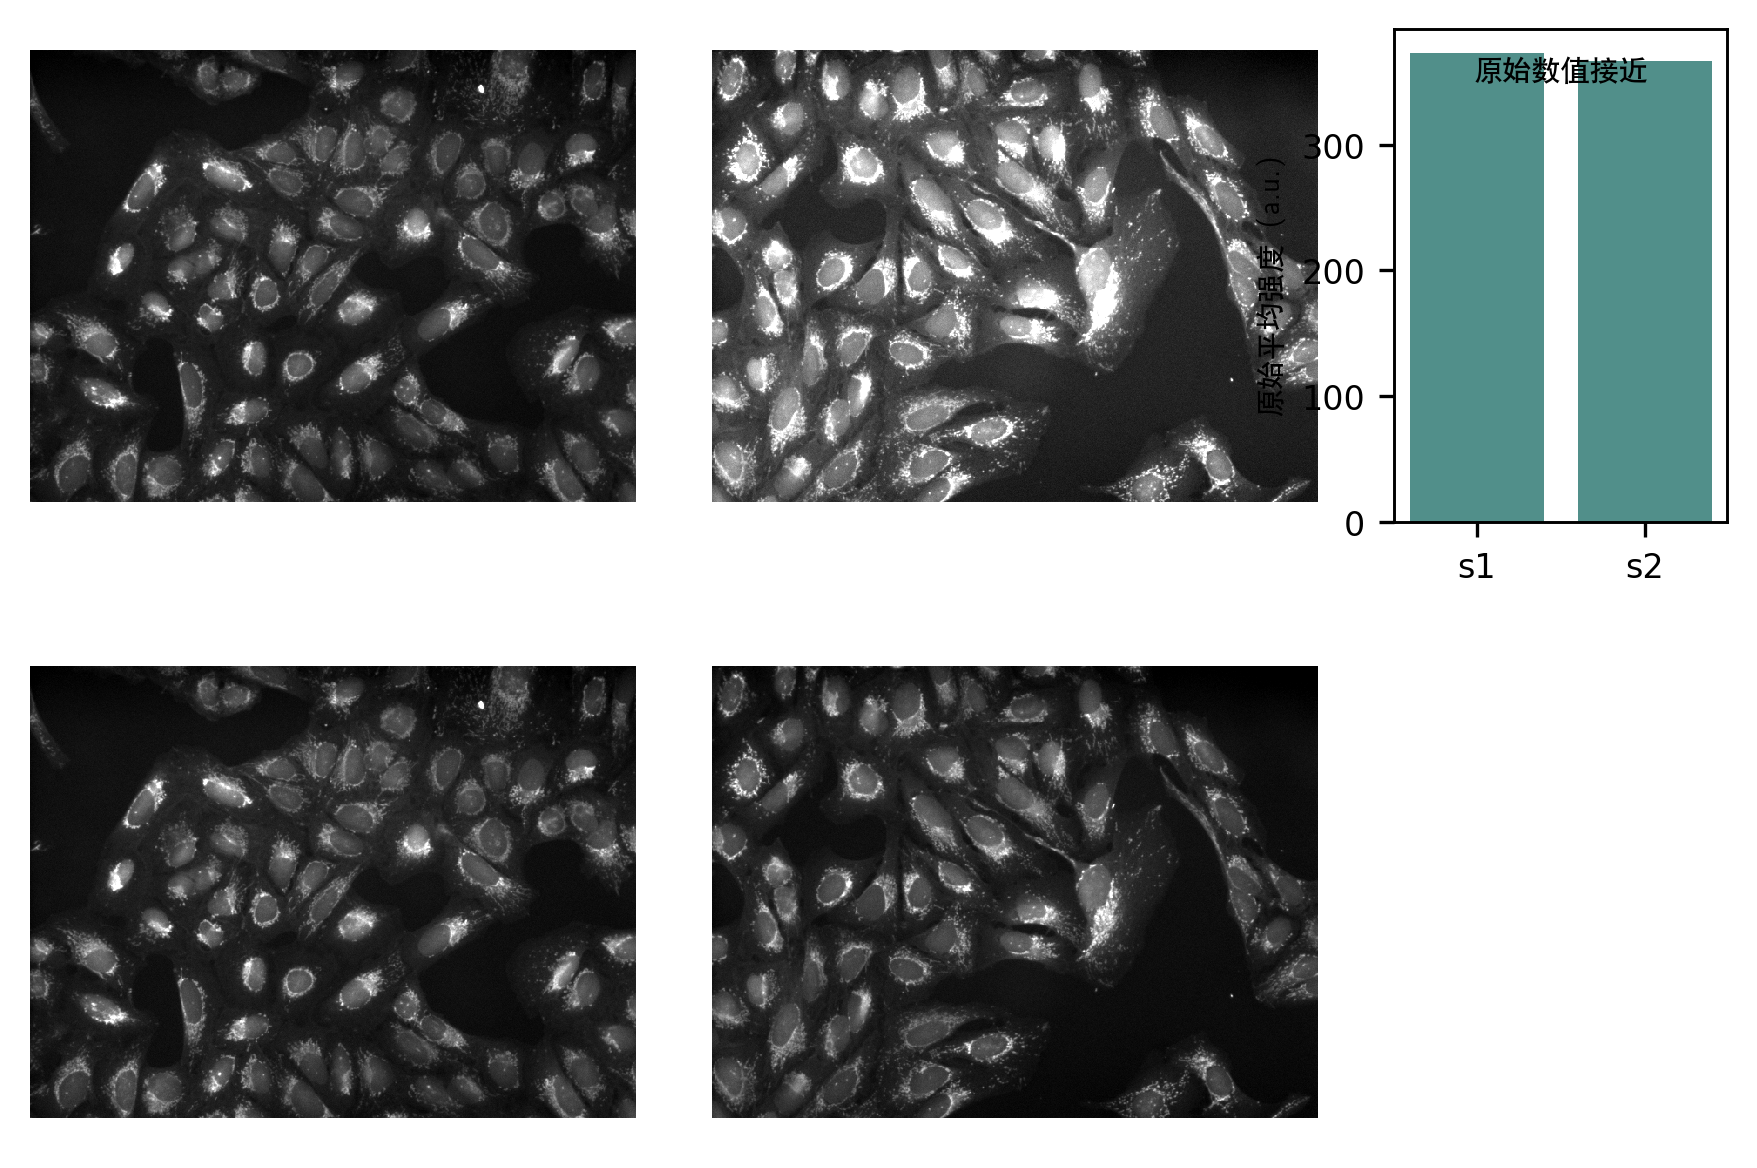
\includegraphics[width=0.88\linewidth]{figures/ch08/ch08-03-consistent-display-zh.png}
\caption{比较面板必须使用相同的显示设置。两幅图来自同一对照孔（BBBC022，孔 A13，视野 1 与 2），没有处理差异。上排分别设置显示范围，右图看似信号更强；下排使用同一显示范围（$218\text{--}1140$），差异消失。右侧为两视野原始平均强度。上排右图的显示范围为教学反例而刻意设定。图像：BBBC022v1，CC0。}\label{fig:ch08-03}
\end{figure}

看图~\ref{fig:ch08-03} 上排的反例：左图 \texttt{s1} 按 $218\text{--}1140$ 映射，右图 \texttt{s2} 刻意将白点压低为 $196\text{--}700$。仅仅因为白点降低了不到四成，上排右图的线粒体就大面积泛白发亮，看似比左图信号强得多；而在下排改用统一的显示范围（$218\text{--}1140$）后，两视野的亮度与染色模式立刻恢复一致。

\section{通道与伪彩色}

荧光显微镜相机对每个波段采集的都是单通道灰度图，论文里看到的彩色是作者指定的伪彩色查找表（LUT）。选择伪彩色时需遵循三条规则：

\textbf{第一，避免红/绿合成，改用品红/绿（或青/品红/黄），并优先提供分通道灰度面板。}男性读者中约有 $8\%$ 存在红绿色觉异常（Wong，2011；Crameri 等，2020）。在传统的红/绿合成图中，纯红与纯绿在红绿色盲读者眼中都会投射为相近的黄褐色，不仅两通道彼此难以区分，连代表共定位的黄色也会融进背景。把红色替换为\textbf{品红色（magenta，将同一通道同时写入红通道 R 与蓝通道 B）}、保留另一通道为\textbf{绿色（写入绿通道 G）}后，第一通道含有强烈的短波蓝光分量，两通道重叠处则叠加为高对比度的白色（$R+G+B$），在两类红绿色盲眼中都能清晰分辨。同时，人眼对单通道灰度的空间细节分辨力高于彩色图（Jambor 等，2021；Schmied 与 Jambor，2020），“分通道灰度 + 品红/绿合成”是最稳妥的组合。

图~\ref{fig:ch08-04} 截取第 1 视野的 $300 \times 300$ 像素区域（坐标 $(198, 110)\text{--}(498, 410)$，显示范围固定为细胞核 $132\text{--}1236$、线粒体 $218\text{--}1140$），在线性 RGB 空间采用 Machado 等（2009）模型（严重度 $1.0$）模拟色觉异常效果。

\begin{figure}[htbp]\centering
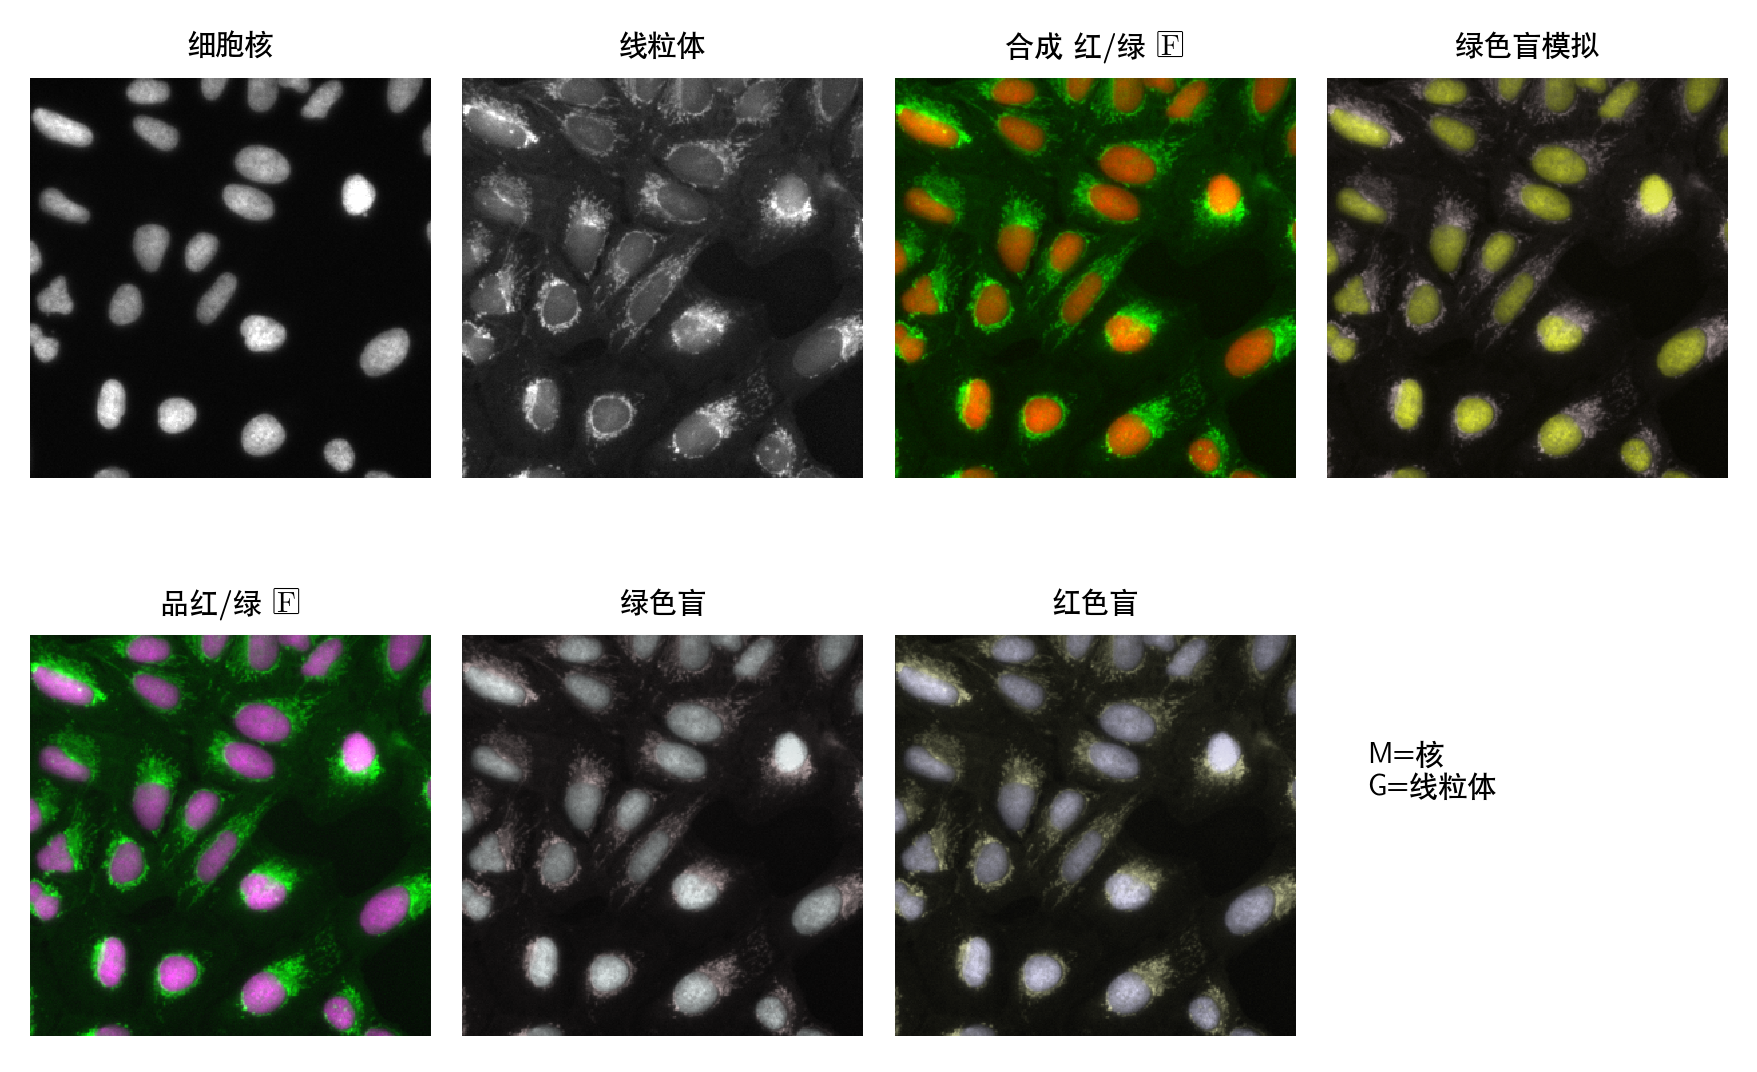
\includegraphics[width=0.88\linewidth]{figures/ch08/ch08-04-pseudocolor-colorblind-zh.png}
\caption{多通道荧光图的伪彩色选择。上排：红/绿合成在绿色盲模拟下两通道难以区分。下排：品红/绿合成在绿色盲与红色盲模拟下仍可区分。单通道灰度图不依赖颜色辨别。色觉模拟采用 Machado 等（2009）模型。图像：BBBC022v1，CC0。}\label{fig:ch08-04}
\end{figure}

对比图~\ref{fig:ch08-04} 上下两排：上排左三的红/绿合成在绿色盲模拟（上排右一）下，细胞核与核周线粒体全部变成相近的暗黄绿色，边界难以剥离；而下排左一的品红/绿合成在绿色盲（下排左二）与红色盲（下排左三）模拟下，浅灰紫色的细胞核与暖橄榄色的线粒体依然界限分明。导出成图后，还可用 \scidraw{} 的图片检查工具（\sdtool{figure-checker}）对整图做色觉风险复查。

\textbf{第二，合成前各通道单独设定线性显示范围并逐一记录。}Nature Portfolio 图像诚信政策规定，合成图中若对单通道做过独立调整须在图注说明。在脚本中先对各 16 位通道按固定 $(v_{\min}, v_{\max})$ 映射为 8 位灰度再合成 RGB，合成后不再做整图调色，即可准确记录并披露参数。

\textbf{第三，扫描电镜（SEM）原本无颜色，人工上色属于伪彩，必须明确声明。}电子显微镜记录的是电子通量强度，原始图像只有灰度。例如达特茅斯学院电镜中心发布在公有领域的混合花粉 SEM 图，原版（\url{https://commons.wikimedia.org/wiki/File:Misc_pollen.jpg}，$1228 \times 935$ 像素）为灰度图，而彩色版（\url{https://commons.wikimedia.org/wiki/File:Misc_pollen_colorized.jpg}）是后期按颗粒轮廓人工涂上的伪彩。作为实验证据呈现时，SEM 图应保持原始灰度；若因说明需要施加伪彩，必须在图注中明确声明。

\section{裁剪、放大与比例尺}

\subsection{保持含义的裁剪与局部放大}

裁剪选区不能变成“挑视野里最亮、最好看的一颗细胞”（Cromey，2010；Jambor 等，2021）。规范的裁剪与局部放大需满足四项要求：
\begin{enumerate}
\item \textbf{选有代表性的区域并写明依据：}例如在展示对照视野时，选取细胞核与线粒体强度均处于视野中位数附近的典型区域，并将选择依据写入处理记录。
\item \textbf{记录精确裁剪框坐标：}将裁剪框在原图中的像素坐标 $(x_0, y_0, x_1, y_1)$ 保存到处理记录中。
\item \textbf{局部放大在母图上标出位置，并优先采用整数倍最近邻插值：}在母图对应位置画出方框（共用同一组像素坐标），写明放大倍数（如 $3\times$）。放大像素块时推荐使用\textbf{最近邻插值（nearest-neighbour）}，把每个原始像素原样扩展为 $3 \times 3$ 同色方块，如实展现相机的空间采样极限，而不使用双三次（bicubic）插值伪造平滑边缘，更不允许“补细节”。
\item \textbf{禁止无缝拼接：}不同视野、时间点或凝胶泳道的图像不得拼成“同一视野”；确需并列须加清晰分隔线并在图注中说明（Rossner 与 Yamada，2004；Bik 等，2016）。
\end{enumerate}

\subsection{从校准信息计算比例尺}

比例尺像素长度等于目标物理长度除以像素物理尺寸：$L_{\text{px}} = L_{\text{phys}} / s_{\text{px}}$；若放大面板做了 $k$ 倍放大，则比例尺像素长度需乘以 $k$ 重新计算：$L'_{\text{px}} = (L'_{\text{phys}} / s_{\text{px}}) \times k$。像素物理尺寸 $s_{\text{px}}$ 只能来自采集元数据、同期拍摄的标准测微尺，或原图底部的\textbf{仪器数据条}。

图~\ref{fig:ch08-05} 以达特茅斯学院电镜中心 Louisa Howard 拍摄的美洲烟草（\textit{Nicotiana alata}）叶片上表皮 SEM 原图（\path{Leaf_epidermis.jpg}，公有领域，$2048 \times 2073$ 像素，8 位灰度）演示比例尺换算、裁剪与局部放大。

\begin{figure}[htbp]\centering
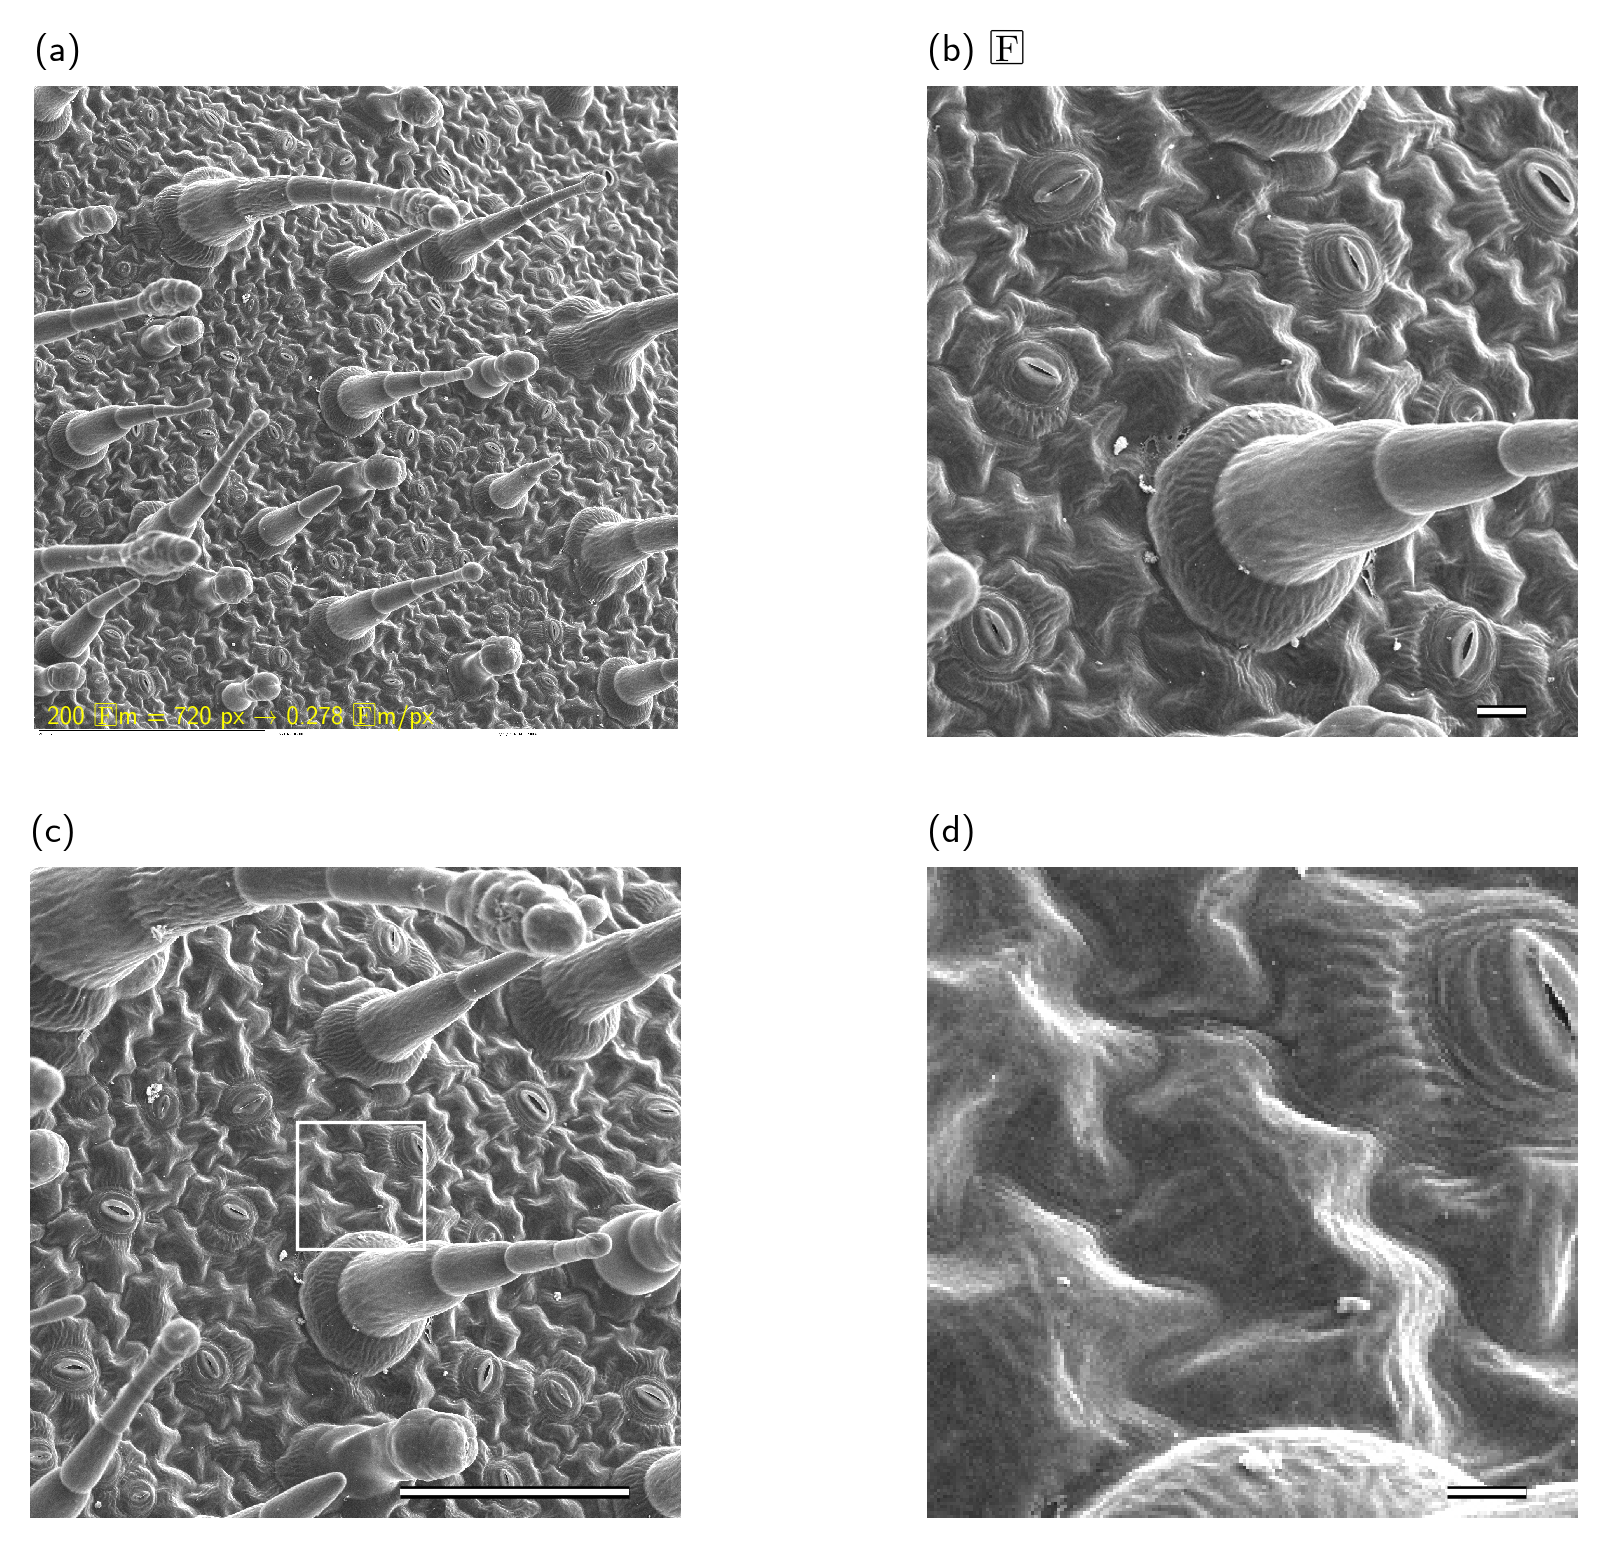
\includegraphics[width=0.88\linewidth]{figures/ch08/ch08-05-crop-inset-scalebar-zh.png}
\caption{裁剪、局部放大与比例尺。(a) 原始 SEM 图像（\textit{Nicotiana alata} 叶上表皮，Zeiss 962，$200\times$），底部为仪器数据条；其中 $200\ \mu\text{m}$ 标尺线长 $720$ 像素，据此像素尺寸为 $0.278\ \mu\text{m}$。(b) 反例：裁掉数据条、只保留个别结构、以双三次插值放大并画上无依据的比例尺。(c) 正确做法：记录裁剪框，按像素尺寸绘制 $100\ \mu\text{m}$ 比例尺；白框区域在 (d) 中以 3 倍最近邻放大，比例尺 $20\ \mu\text{m}$。图像：Louisa Howard, Dartmouth Electron Microscope Facility，公有领域。}\label{fig:ch08-05}
\end{figure}

对照图~\ref{fig:ch08-05} 的四个面板：
\begin{itemize}
\item \textbf{面板 (a)（从原图仪器数据条实测像素尺寸）：}原图底部 $25$ 行像素（行号 $2048\text{--}2072$）为蔡司 DSM 962 电镜自动生成的白色数据条，印有标尺线及“\texttt{200 um}”“\texttt{200X}”“\texttt{7/31/3 REMF}”“\texttt{Nict.\ leaf \#2.001}”。脚本自动扫描数据条区域的水平暗像素连续游程（灰度 $<80$），测得第 $2052\text{--}2053$ 行、$x = 15\text{--}734$ 的黑色标尺线精确跨越 \textbf{$720$ 像素}，由此算得 $s_{\text{px}} = 200\ \mu\text{m} / 720\ \text{px} \approx 0.2778\ \mu\text{m/px}$（依赖仪器放大率标定，图注写明“据仪器数据条换算”）。此外，Wikimedia Commons 上另有第三方裁掉数据条并另加“$200\ \mu\text{m}$”白线的派生图（\path{Leaf_epidermis_w_scale.jpg}，$2048 \times 2052$ 像素）。使用第三方派生图时必须回到原图核对——我们实测该派生图白线（$x=240\text{--}959$）长 $720$ 像素，与原图数据条一致，这就是“回原图核对”的示范。
\item \textbf{面板 (b)（反例）：}裁掉底部数据条，只截取中央一根毛状体（$600 \times 600$ 像素）做 $4\times$ 双三次插值放大，并在右下角随手画了一根标称“$50\ \mu\text{m}$”、实为正确换算长度 2 倍的无依据比例尺。
\item \textbf{面板 (c) 与 (d)（正确做法）：}面板 (c) 记录 $1024 \times 1024$ 像素裁剪框 $(480, 320)\text{--}(1504, 1344)$，绘制 $100\ \mu\text{m} = 360\ \text{px}$ 比例尺，并用白框标出 $200 \times 200$ 像素的气孔区域 $(900, 720)\text{--}(1100, 920)$；面板 (d) 将白框区域做 $3\times$ 最近邻放大，比例尺按放大倍数重算为 $20\ \mu\text{m} = 72 \times 3 = 216\ \text{px}$。
\end{itemize}

\subsection{没有校准信息就不画比例尺}

如果图像没有记录像素尺寸，也没有仪器数据条，唯一合规的做法是\textbf{不画比例尺，并在图注中写明“像素尺寸未知”}——绝不能按“细胞看起来大约 $20\ \mu\text{m}$”去估画。

图~\ref{fig:ch08-06} 展示了来自 ImageJ 示例集的三通道荧光图（\path{FluorescentCells.jpg}，牛肺动脉内皮细胞，蓝 DAPI、绿微管、红 F-actin，公有领域，$512 \times 512$ 像素；同时也是第 3 节红/绿共存合成的反例）：该文件以 8 位有损 JPEG 合成图发布，JFIF 密度为无单位的 $1:1$，来源页未给物镜与像素尺寸（面板 a）。面板 (b) 凭印象加比例尺属于编造尺度；面板 (c) 不画比例尺并标明“未校准”才是正确做法；面板 (d) 将局部 $(200, 200)\text{--}(280, 280)$ 做 $4\times$ 最近邻放大，清晰可见 $8 \times 8$ JPEG 块状伪影与通道串色，说明该文件只能作为定性显示图，不能当作原始测量数据。

\begin{figure}[htbp]\centering
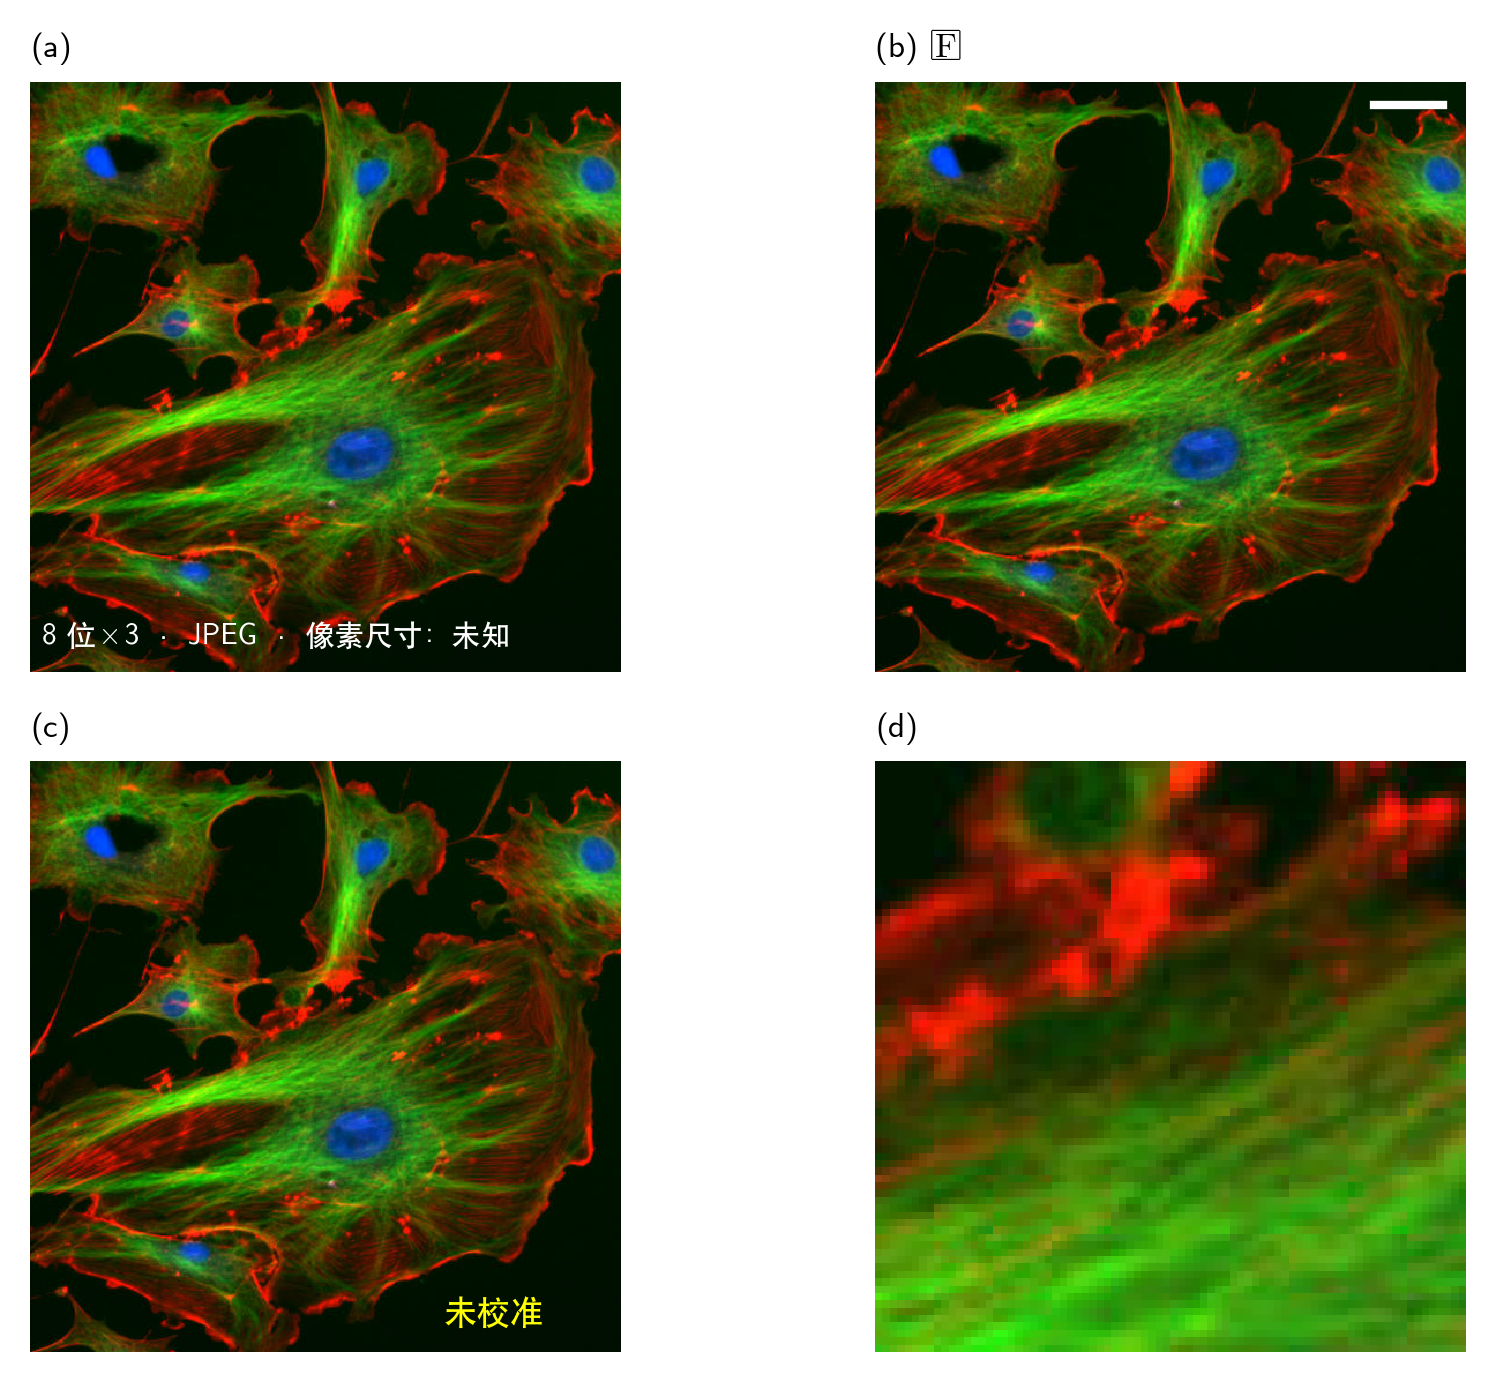
\includegraphics[width=0.88\linewidth]{figures/ch08/ch08-06-no-calibration-zh.png}
\caption{没有校准信息时不画比例尺。(a) 来自 ImageJ 示例集的三通道荧光图（牛肺动脉内皮细胞；蓝 DAPI、绿微管、红 F-actin），以 8 位 JPEG 合成图发布，未记录像素尺寸。(b) 反例：凭印象添加的比例尺。(c) 正确做法：不画比例尺，并在图注中写明“像素尺寸未知”。(d) 局部放大可见 JPEG 压缩块，说明此文件只能作为显示图，而不是原始测量数据。图像：公有领域（Wikimedia Commons，FluorescentCells.jpg）。}\label{fig:ch08-06}
\end{figure}

\section{期刊规则与 AI 的边界}

\textit{Journal of Cell Biology}（Rossner 与 Yamada，2004）提出的经典规则与 Cromey（2010）的伦理准则共同确立了科学数字图像的底线：整图调整亮度、对比度或色彩平衡是可接受的（非线性调整须在图注披露），但\textbf{图像中的任何特定特征均不得被增强、遮蔽、移动、移除或引入}。Bik 等（2016）对 20,621 篇生物医学论文的筛查发现约 $3.8\%$ 存在不当图像重复或操作，促使主流期刊在出版前全面引入图像取证检查。

在生成式 AI 时代，Nature Portfolio《图像诚信与标准》与 Springer Nature《人工智能（AI）政策》（均于 2026 年 10 月 29 日访问；该政策更新频繁，正文引用与投稿前均须核对最新文本）进一步规定：调整须整图且对照同等施加，不得让数据消失，伪彩与 $\gamma$ 等非线性调整以及合成图中的单通道调整均须在图注说明，禁止克隆与修复工具，并把\textbf{“伪造数据、引用或结果”与“生成照片级图像（deepfakes）”明确列为不允许}。

为什么不能把模糊的实验图像交给生成式模型“去噪、变清晰”？我们在图~\ref{fig:ch08-05} 所用的烟草叶表皮 SEM 原图上做了一个有真实地面真值（GT）的对照实验（图~\ref{fig:ch08-07}）：
\begin{enumerate}
\item 从原图截取 $512 \times 512$ 像素区域 $(640, 680)\text{--}(1152, 1192)$ 作为\textbf{地面真值 GT}（面板 a），内含三处气孔、表皮细胞边界、右侧大毛状体基部与左下斜向小毛状体。
\item 按 $4 \times 4$ 区域平均降采样为 $128 \times 128$ 像素低分辨图 \textbf{LR}（面板 b，最近邻显示）。
\item \textbf{对照 1（面板 c）：}将 LR 用双三次插值放大回 $512 \times 512$ 像素（确定性插值，模糊但不添加新结构）。
\item \textbf{对照 2（面板 d）：}将同一张 $128 \times 128$ 的 LR 图传入图像生成模型的编辑模式，按普通用户常见的英文提示词独立运行 3 次（为避免挑选最离谱的一次，正文固定使用第 1 次结果，其余两次存档）：
\end{enumerate}

\begin{Prompt}
Upscale this grayscale scanning electron microscope image to 512 x 512 pixels.
Make it sharper and more detailed, remove blur and noise, and enhance the fine
surface structures so it looks like a high-resolution micrograph.
Keep it grayscale. Do not add any text, letters, numbers, labels, or scale bars.
Square 1:1 aspect ratio.
\end{Prompt}

\begin{figure}[htbp]\centering
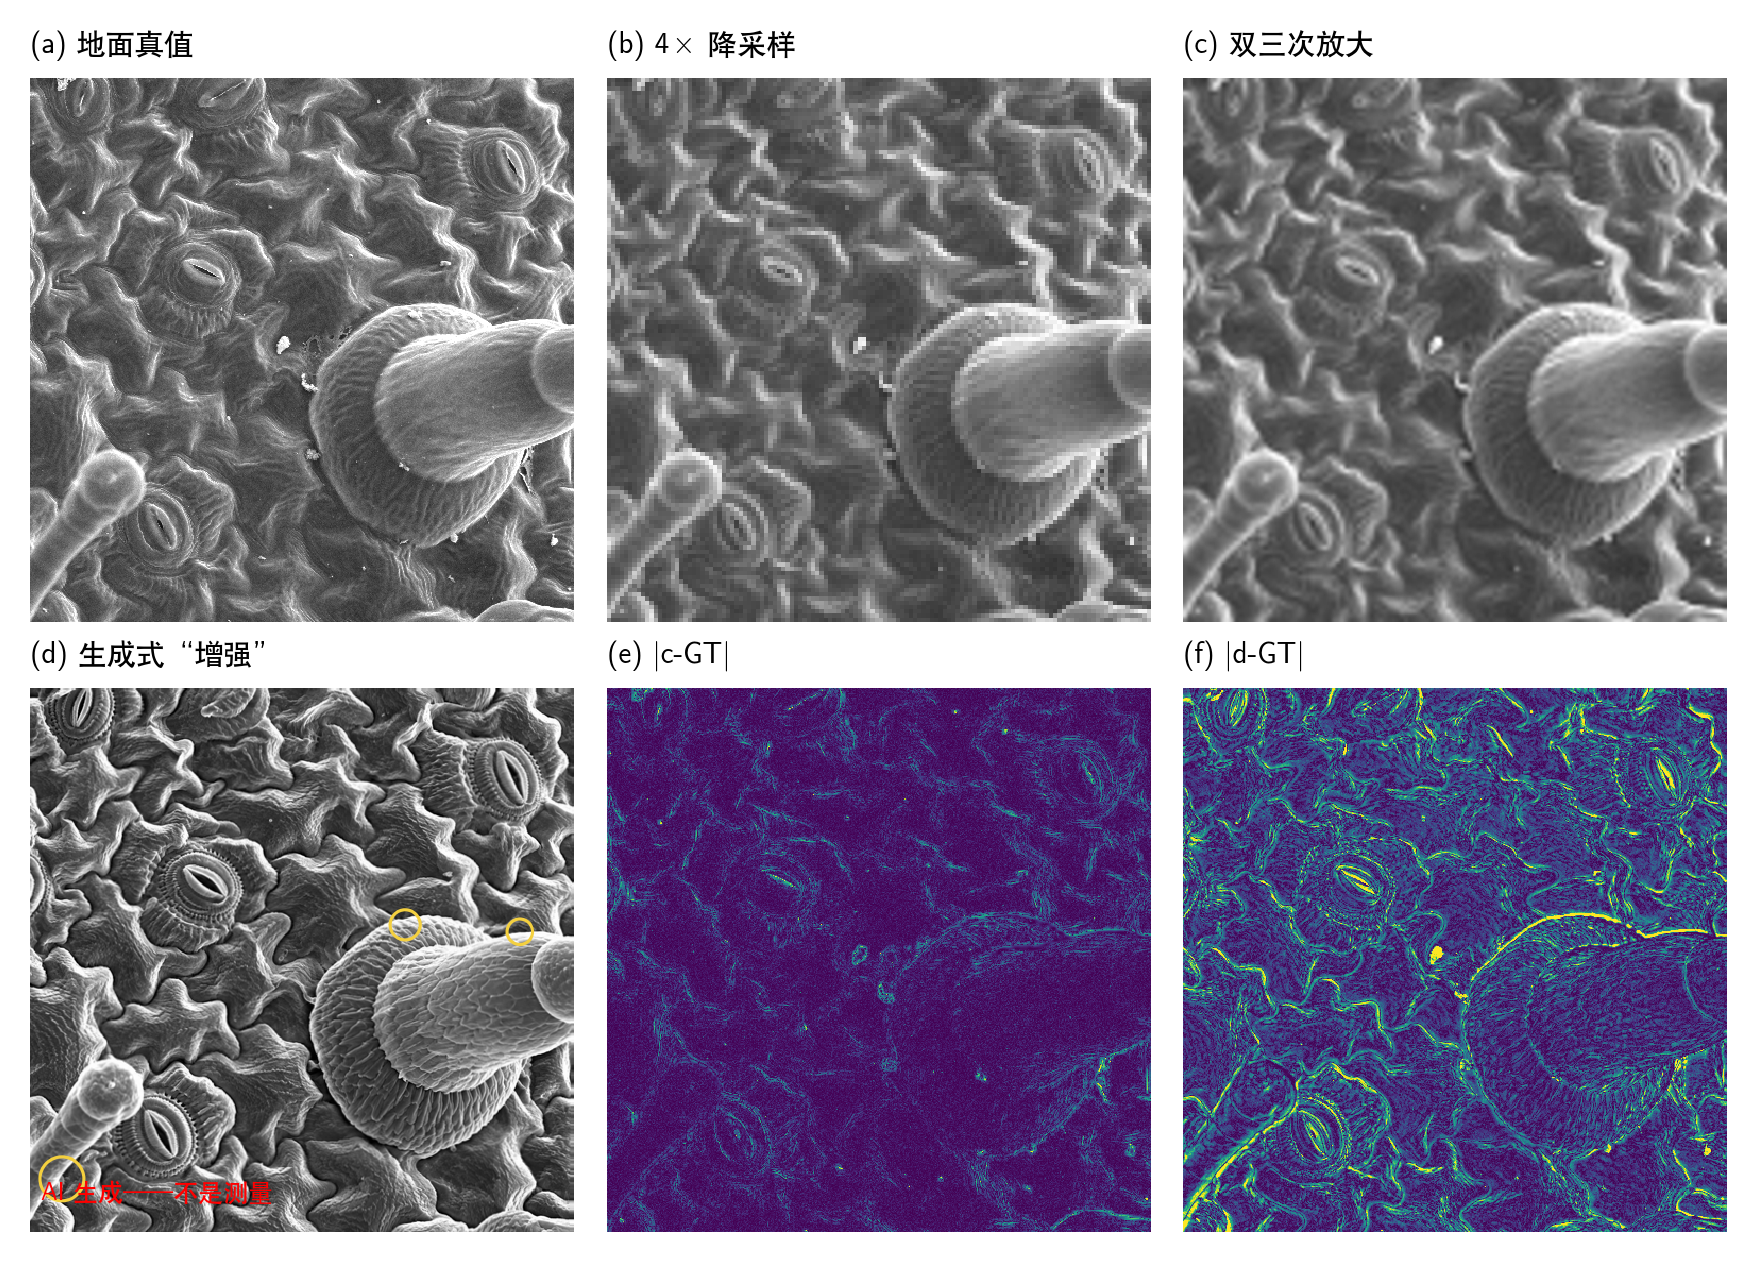
\includegraphics[width=0.88\linewidth]{figures/ch08/ch08-07-generative-risk-zh.png}
\caption{生成式“增强”会编造结构。(a) SEM 原图局部（地面真值）。(b) 将其 4 倍降采样后的低分辨率版本。(c) 双三次插值放大：图像模糊，但没有新增结构。(d) 用图像生成模型按“变清晰、增强细节”的要求放大：看起来更清晰，却含有原图中不存在的边界与纹理（圆圈处）。(e)、(f) 分别为 (c)、(d) 与原图的绝对差。生成图仅用于说明风险，不能作为实验图像使用。原图：Louisa Howard, Dartmouth Electron Microscope Facility，公有领域；面板 (d) 由图像模型生成，提示词与生成记录见本书仓库。}\label{fig:ch08-07}
\end{figure}

对比图~\ref{fig:ch08-07} 的六个面板与三次生成结果，可以看到生成式“增强”的四重失真（本实验不评测某一特定产品，任何生成式放大模型都有同类风险）：
\begin{itemize}
\item \textbf{像素尺寸与通道属性失控：}提示词明确要求输出 $512 \times 512$ 单通道灰度图，但三次调用实际返回的全部是 $1254 \times 1254$ 像素（约为输入边长 $9.8$ 倍）的三通道 8 位 RGB 图，且 RGB 三通道间存在最大 $10\text{--}12$ 灰阶的差值，并非严格单通道灰度。
\item \textbf{凭空捏造原图中不存在的边界与纹理：}面板 (d) 看似比双三次插值 (c) 清晰得多，但与地面真值 (a) 逐区对照可见：左上气孔开口外围被编造出规则的多层环形边缘与齿状纹理，右侧大毛状体及表皮铺满了原图并不存在的紧密鳞片状细纹；在面板 (d) 用三个黄色圆圈标出的位置——大毛状体基部上缘的两处褶皱脊线（中心约 $(353, 222)$ 与 $(460, 229)$）和左下小毛状体顶端（中心约 $(30, 461)$）——模型均画出了原图中不存在的亮边与结构边界。
\item \textbf{多次生成之间细节互相矛盾：}同一张 $128 \times 128$ 输入图独立生成三次，第 1 次表面是紧密条片纹，第 2 次变成更圆钝密集的卵石状颗粒且左下毛状体顶端裂成多边形分块，第 3 次又在大毛状体基部画出放射状细长褶片。这证明新出现的高频细节并非来自样品测量，而是模型随机填充的纹理。
\item \textbf{逐像素绝对误差接近双三次插值的 3 倍：}将第 1 次生成输出转为灰度、仅因比较需要用 Lanczos 缩回 $512 \times 512$，再做一次刚性配准（旋转 $-0.5^\circ$，平移 $dx=-1, dy=+1$ 像素）以消除轻微几何错位，计算与地面真值 GT 的绝对差（面板 e、f，统一采用 $0\text{--}128$ 的 \texttt{viridis} 色标）。双三次插值 $|c - \text{GT}|$（面板 e）的平均绝对误差（MAE）仅为 $10.32$ 灰阶；而生成式放大 $|d - \text{GT}|$（面板 f）配准后的 MAE 高达 $28.91$ 灰阶（配准前为 $29.06$），画面布满亮黄与亮绿色误差带。
\end{itemize}

结论只有一条：\textbf{AI 可以帮你写处理脚本、写方法、查色觉，但不能产生任何一个将被当作测量的像素。}

\section{完整案例：U2OS 细胞对照视野的呈现}

现在我们把小苏的补充材料方法图完整走一遍。本图用于在论文补充材料中展示 DMSO 对照（\texttt{mock}）条件下 U2OS 细胞的细胞核与线粒体染色模式，让同行判断后续定量分析所用原始图像的质量。本图\textbf{不报告任何处理效应}；由于使用公开基准数据集 BBBC022v1（Gustafsdottir 等，2013），采集参数严格引用数据集说明（$20\times$ 物镜，$0.656\ \mu\text{m/pixel}$）与原始论文，不自行补写未知参数。

\textbf{第一步：建立原图目录（交付物 1）。}将孔 A13 视野 \texttt{s1}、\texttt{s2} 的四个 16 位 TIFF 设为只读，由脚本校验 SHA-256 并生成原图目录（表~\ref{tab:ch08-catalog}，同时导出为同名 CSV）。

\begin{table}[htbp]\centering\footnotesize
\setlength{\tabcolsep}{3pt}
\renewcommand{\arraystretch}{1.15}
\caption{主案例原图目录（以视野 1 两通道为例；视野 2 的 \texttt{w1} 范围 $122\text{--}1450$、均值 $227.1$、$p_{0.1}/p_{99.9}=129/1150$，\texttt{w5} 范围 $176\text{--}1655$、均值 $366.3$、$p_{0.1}/p_{99.9}=196/1078$，一并收入目录 CSV）。}\label{tab:ch08-catalog}
\begin{tabularx}{\linewidth}{@{}>{\raggedright\arraybackslash}p{25mm}YY@{}}
\toprule
\textbf{字段} & \textbf{示例：s1 Hoechst（w1）} & \textbf{示例：s1 MitoTracker（w5）} \\
\midrule
文件名 & \path{IXMtest_A13_s1_w1B35C6D5D-DBF9-4779-990D-5E7AFB14D600.tif} & \path{IXMtest_A13_s1_w5B257EE32-37B0-4698-891B-11B1B3D3D0C1.tif} \\
来源 & BBBC022v1，板 20585，孔 A13（\texttt{mock}），视野 1 & BBBC022v1，板 20585，孔 A13（\texttt{mock}），视野 1 \\
通道 / 染料 & w1 / Hoechst 33342（DNA） & w5 / MitoTracker Deep Red（线粒体） \\
尺寸 / 位深 & $696 \times 520\ \text{px}$，16 位容器，12 位有效 & $696 \times 520\ \text{px}$，16 位容器，12 位有效 \\
像素尺寸 & $0.656\ \mu\text{m}$（数据集说明，$20\times$） & $0.656\ \mu\text{m}$（数据集说明，$20\times$） \\
SHA-256 前 16 位 & \texttt{4be40f814481002a}（全长 64 位见目录 CSV） & \texttt{c1c441e44e91481c}（全长 64 位见目录 CSV） \\
原始数值范围 & $121\text{--}1655$；$p_{0.1}/p_{99.9}=132/1236$；饱和像素 $0$ & $185\text{--}4095$；$p_{0.1}/p_{99.9}=218/1140$；饱和像素 $12$ \\
许可与处理状态 & CC0 1.0；只读原件，所有处理在副本上进行 & CC0 1.0；只读原件，所有处理在副本上进行 \\
\bottomrule
\end{tabularx}
\end{table}

\textbf{第二步：编写任务书（交付物 2）。}在 \scidraw{} 科研绘图向导（\sdtool{figure-workflow}）中选择“已有图片组图”路线，编写并保存任务书：

\begin{Prompt}
【用途与读者】论文补充材料方法图（Supplementary Figure），双栏宽 174 mm；
读者为做细胞成像的同行，需要判断原始图像与染色模式的质量。
【目标】展示 DMSO 对照条件下 U2OS 细胞的细胞核（Hoechst 33342）与线粒体
（MitoTracker Deep Red）染色模式；不报告任何处理效应。
【材料】BBBC022v1（CC0），板 20585，孔 A13（mock），视野 s1；通道 w1、w5；
16 位 TIFF，696 × 520 px，0.656 µm/pixel（数据集说明）。原件只读，SHA-256 见目录。
【面板】a 细胞核（灰度）；b 线粒体（灰度）；c 合成图（细胞核品红、线粒体绿）；
d 为 c 中一个区域的局部放大（在 c 上用方框标出位置）。
【处理】只允许：整图线性显示范围（黑点/白点）、伪彩色映射、裁剪、整数倍最近邻放大。
每个通道一套显示范围，所有面板共用；数值写入处理记录。
不允许：伽马（gamma）或曲线、去噪、锐化、反卷积、背景扣除、局部调整、生成式“增强”。
【比例尺】按 0.656 µm/pixel 计算：a–c 用 50 µm，d 按放大后重新计算 10 µm；
画在面板右下，白色实线，图注写明长度，面板内不写数字以免拥挤。
【选区与饱和】d 选核与线粒体信号均在视野中位附近的典型细胞；线粒体通道原始数据有
12 个像素为 4095（采集时饱和），在处理记录中报告，不做修补。
【导出与验收】面板导出无损 8 位 PNG，在 SciDraw AI 组图工具排版并导出 TIFF/PDF 与处理记录；
各面板能追溯 SHA-256，比例尺可复算，红绿色盲模拟下两通道可区分，图注含显示设置与饱和说明。
\end{Prompt}

\textbf{第三步：用通用 AI 对话助手整理呈现计划与起草处理脚本。}向通用 AI 对话助手提交如下提示词（这一步用于生成计划与确定性 Python 脚本，而非调用图像生成工具）：

\begin{Prompt}
我有一组荧光显微原始图像，需要做论文补充材料的展示图。请先不要写代码，
先按下列信息给出“呈现计划”：每个面板显示什么、每一步处理是否属于线性操作、
每一步需要在处理记录或图注中写什么。
图像：两个 16 位 TIFF，696 × 520 px，单通道灰度；
w1 = Hoechst 33342（细胞核），w5 = MitoTracker Deep Red（线粒体）；
像素尺寸 0.656 µm（数据集说明）；原始数值为 12 位，w5 有 12 个饱和像素（4095）。
要求：
1. 只用整图线性显示范围；黑点/白点由原始数值的分位数给出，并输出具体数值。
2. 合成图用品红（细胞核）和绿（线粒体），说明为什么不用红/绿。
3. 比例尺长度由像素尺寸计算，给出像素数；放大面板要重新计算。
4. 列出不允许做的处理（去噪、锐化、伽马 gamma、局部调整、生成式增强）。
5. 最后列出我必须人工核对的项目。
计划确认后，再写一个 Python 脚本（numpy、tifffile 或 PIL、matplotlib），
要求：读取原件但不覆盖；打印并保存每个面板的显示范围、裁剪框、放大倍数、
比例尺像素数和输入文件 SHA-256 到 processing-log.json。
\end{Prompt}

提醒：AI 在对话中给出的分位数或像素数不能直接采信，必须由脚本在真实数据上算出并回填，不能采用对话里“估计”的数字；脚本须先在副本上运行，并人工检查代码确认没有调用任何去噪、锐化或伽马函数。

\textbf{第四步：检查初稿（v1）的五个问题并下达修改指令。}图~\ref{fig:ch08-08} 展示了模拟“顺手做”生成的初稿反例，图中叠加的编号 1–5 标出了五处典型问题：
\begin{enumerate}
\item \textbf{问题 1（各自自动对比度）：}a、b 两个面板各自按 \texttt{min--max} 自动拉伸，c 合成图又不一致，无法记录为一组统一参数。
\item \textbf{问题 2（红/绿合成）：}合成图采用红/绿配色，红绿色觉异常模拟下两通道难以区分。
\item \textbf{问题 3（比例尺无依据）：}c 右下角“照着别的图画了一个 $20\ \mu\text{m}$”，实际像素长度为 $50\ \text{px}$，而按 $0.656\ \mu\text{m/px}$ 计 $20\ \mu\text{m}$ 应为 $30.5\ \text{px}$——比例尺偏长 $64\%$。
\item \textbf{问题 4（最亮细胞 + 双三次插值）：}放大面板 d 挑了视野中最亮、形态最特殊的那颗细胞核 $(488, 184)\text{--}(552, 248)$，用双三次插值放大 $4\times$，且未在 c 上标出选区位置。
\item \textbf{问题 5（未披露 $\gamma = 0.6$ 与有损导出）：}线粒体通道施加了 $\gamma = 0.6$ 让弱信号显得更亮但未披露，并以质量 $70$ 的 JPEG 导出。
\end{enumerate}

\begin{figure}[htbp]\centering
\resizebox{0.88\linewidth}{!}{% FIG ch08-08 v1 issue overlay (Chinese).
% Numbered marks sit on the panel each problem belongs to.
% The phrases are listed under the micrograph so they do not cover it.
\tikzset{%
  chviiiissue/.style={%
    circle, draw=BookInk, line width=0.4pt, fill=white, inner sep=0.2pt,%
    minimum size=9pt, font=\sffamily\fontsize{7}{8}\selectfont, text=BookInk%
  },%
  chviiicap/.style={%
    anchor=west, inner xsep=0.4pt, inner ysep=0.5pt,%
    font=\sffamily\fontsize{7}{9}\selectfont, text=BookInk%
  }%
}
\providecommand{\chviiimark}[1]{%
  \tikz[baseline=(n.base)]{\node[chviiiissue] (n) {#1};}%
}
\begin{tikzpicture}
  \node[anchor=south west, inner sep=0pt] (img) at (0,0)
    {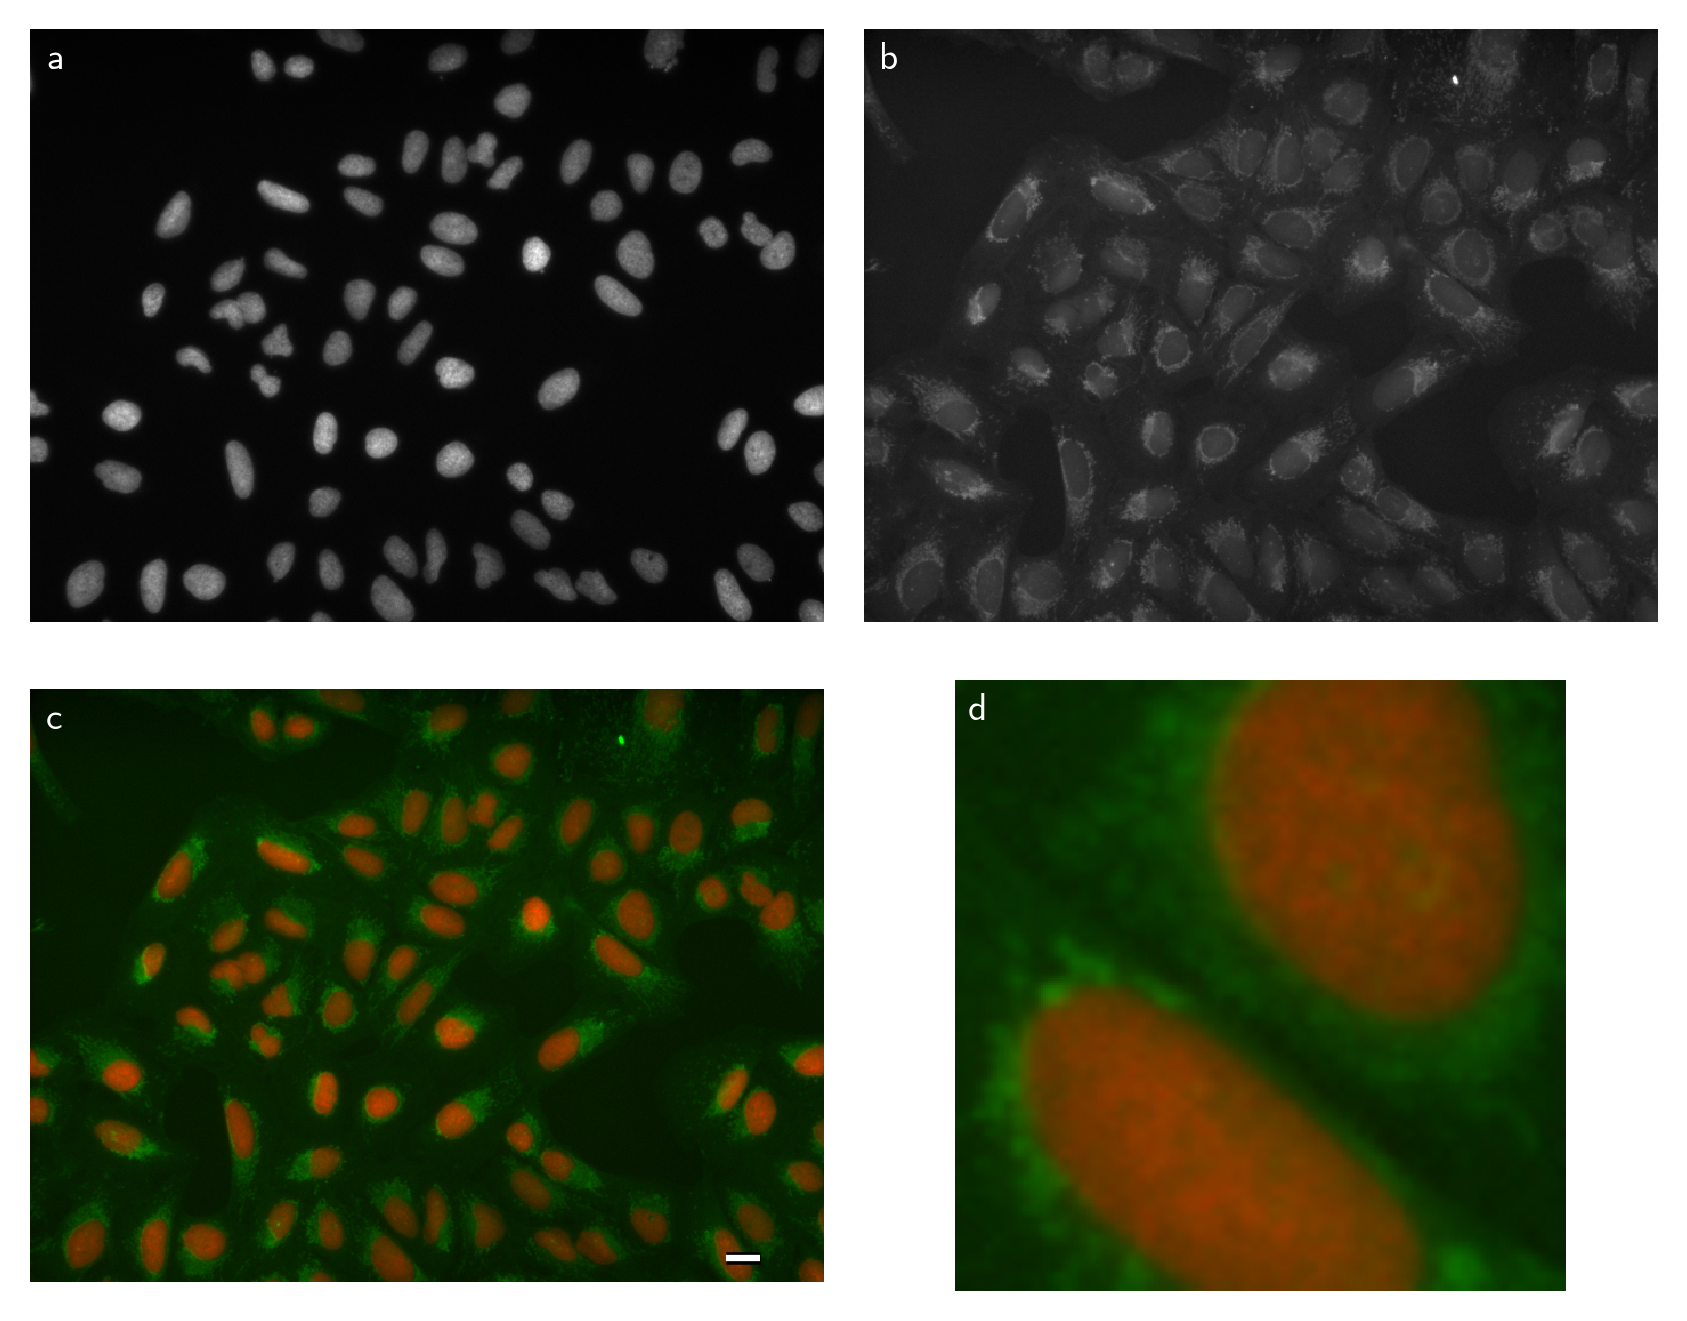
\includegraphics[width=\linewidth]{figures/ch08/ch08-08-case-v1-zh.png}};
  \begin{scope}[x={(img.south east)}, y={(img.north west)}]
    \node[chviiiissue] (m1) at (0.40, 0.92) {1};
    \node[chviiiissue] (m2) at (0.40, 0.45) {2};
    \node[chviiiissue] (m3) at (0.36, 0.09) {3};
    \draw[BookInk, line width=0.35pt] (0.372, 0.078) -- (0.424, 0.056);
    \node[chviiiissue] (m4) at (0.88, 0.12) {4};
    \node[chviiiissue] (m5) at (0.90, 0.92) {5};
  \end{scope}
  \node[chviiicap] (c1) at ([yshift=-1.8mm]img.south west)
    {\chviiimark{1}\enspace 各自自动对比度};
  \node[chviiicap] (c2) at ([yshift=-0.8mm]c1.south west)
    {\chviiimark{2}\enspace 红/绿};
  \node[chviiicap] (c3) at ([yshift=-0.8mm]c2.south west)
    {\chviiimark{3}\enspace 比例尺无依据};
  \node[chviiicap] (c4) at ([yshift=-0.8mm]c3.south west)
    {\chviiimark{4}\enspace 最亮细胞+双三次};
  \node[chviiicap] (c5) at ([yshift=-0.8mm]c4.south west)
    {\chviiimark{5}\enspace 未披露 $\gamma=0.6$};
\end{tikzpicture}
}
\caption{初稿中常见的五个问题（编号 1–5，见正文）。本图为按错误做法刻意生成的教学反例。终稿图注见案例小节。}\label{fig:ch08-08}\label{fig:ch08-08-v1}
\end{figure}

对照上述五处问题，列出逐条可核对的修改单：

\begin{Prompt}
修改单（v1 -> final）
1. 两个通道各用一套显示范围，所有面板共用：
   Hoechst 黑点 132、白点 1236（原始数值 p0.1 / p99.9）；
   MitoTracker 黑点 218、白点 1140（p0.1 / p99.9）。合成图使用同一组数值。
2. 取消伽马（gamma），全部为线性映射；处理记录写入“线性，无 gamma”。
3. 合成改为细胞核品红（R+B）、线粒体绿（G）；做一次红绿色盲模拟检查。
4. 比例尺按 0.656 µm/pixel 重算：50 µm = 76.2 px（a–c）；
   d 为 3× 最近邻放大，10 µm = 15.2 px × 3 = 45.7 px。
5. d 的选区改为一个核与线粒体信号都接近视野中位的细胞（坐标 (280, 328)–(344, 392)），
   在 c 上用 0.5 pt 白色方框标出；记录裁剪框像素坐标。
6. 放大用整数倍最近邻（3×），不使用双三次或任何“细节增强”。
7. 导出无损 PNG；保留原始 16 位 TIFF 与脚本、processing-log.json。
8. 在处理记录与图注中报告：线粒体通道有 12 个像素在采集时饱和（4095）。
\end{Prompt}

\textbf{第五步：在 \scidraw{} 组图工具排版、合并双层处理记录并完成终稿核验。}脚本按修改单生成四个 8 位无损 PNG 面板与 \path{processing-log.json} 后，进入 \scidraw{} 组图工具（\sdtool{multi-panel-figure-maker}）：导入四个面板，选择期刊双栏预设（Cell 或 Springer 双栏宽 $174\ \text{mm}$），设为 $2 \times 2$ 网格并自动编号 \textbf{a}--\textbf{d}（在组图工具内做的必要裁剪或旋转也会被自动记录），导出 ZIP 包（含 TIFF、PNG、PDF、PPTX 与组图处理记录），得到终稿（图~\ref{fig:ch08-09}）。

\begin{figure}[htbp]\centering
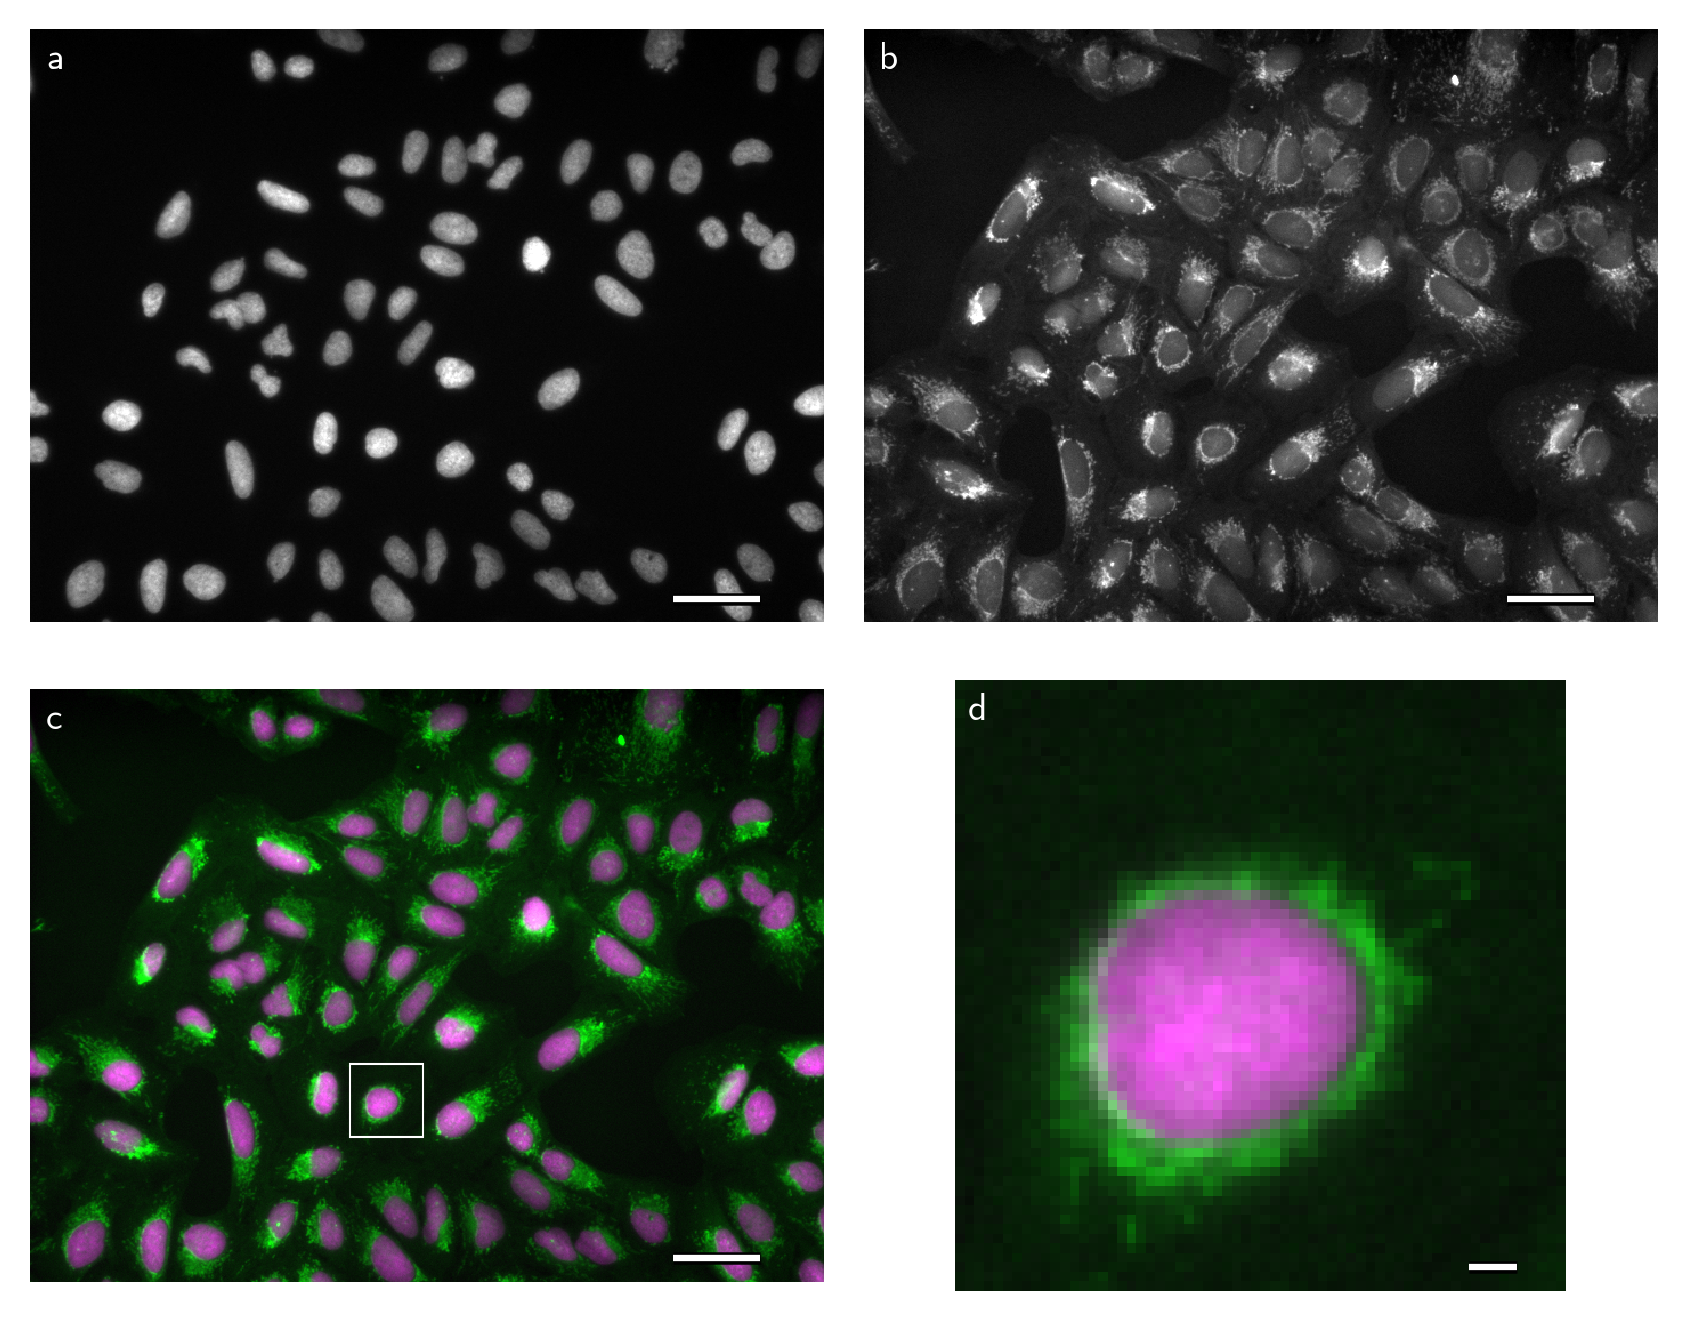
\includegraphics[width=0.88\linewidth]{figures/ch08/ch08-08-case-final-zh.png}
\caption{补充图 S1 | DMSO 对照条件下 U2OS 细胞的细胞核与线粒体染色。\textbf{a}，Hoechst 33342（细胞核）；\textbf{b}，MitoTracker Deep Red（线粒体）；\textbf{c}，合成图（细胞核品红，线粒体绿），白框为 d 的取样区域；\textbf{d}，c 中白框区域 3 倍最近邻放大。图像来自 BBBC022v1（板 20585，孔 A13，视野 1；CC0；Gustafsdottir 等，2013），$20\times$ 物镜，像素尺寸 $0.656\ \mu\text{m}$。所有面板为整图线性显示映射，无 $\gamma$ 或其他非线性调整；Hoechst 显示范围 $132\text{--}1236$、MitoTracker $218\text{--}1140$（原始 12 位数值），同一通道在各面板中设置相同。线粒体通道有 12 个像素在采集时达到饱和（$4095$），未做修补。比例尺：a--c 为 $50\ \mu\text{m}$，d 为 $10\ \mu\text{m}$。原始 16 位图像、处理脚本与处理记录见补充数据。}\label{fig:ch08-09}\label{fig:ch08-08-final}
\end{figure}

在这一步，作者必须特别注意两项平台边界与核验要点：
\begin{enumerate}
\item \textbf{合并上游处理记录与组图处理记录：}组图工具导出的处理记录会列出每个面板的原文件名、SHA-256、原始尺寸与位深、裁剪框、旋转/翻转、在图中的毫米尺寸、有效分辨率和重采样方式，并写明“除上述裁剪、旋转与缩放外，未对任何面板做亮度、对比度、颜色或内容改动”。必须明确：\textbf{这句声明只描述组图工具内部的操作。}由于导入的 PNG 面板已经在上游脚本中经过了显示范围映射与伪彩色合成，且组图工具当前不提供校准比例尺、通道标签与关联放大框功能（这些均在脚本中完成），导出 ZIP 也不包含原始 16 位 TIFF，作者必须把脚本生成的 \path{processing-log.json} 与组图处理记录\textbf{合并}成一份完整处理说明，否则读者会误以为面板未经任何显示调整。
\item \textbf{如实核查有效分辨率与补齐图注：}$696\ \text{px}$ 宽的原图在 $300\ \text{dpi}$ 下约为 $59\ \text{mm}$；在 $174\ \text{mm}$ 宽的 $2 \times 2$ 布局中每格约 $85\ \text{mm}$ 宽，此时有效分辨率约为 $208\ \text{dpi}$。对此，作者要么接受较低的有效分辨率并在说明中如实写出原始像素尺寸，要么缩小面板物理尺寸以达到 $300\ \text{dpi}$，\textbf{绝不能用插值放大冒充分辨率}。随后用图片检查工具（\sdtool{figure-checker}）检查导出图的格式、分辨率、灰度与色觉风险（注意它只做技术检查，不代表科学审核）；再用图注辅助工具（\sdtool{figure-legend}）起草“看图可见”的描述，由作者亲手补齐染料、像素尺寸、显示范围、饱和说明与比例尺长度（工具按设计不编造放大倍数、比例尺或方法）。终稿对应的英文图注与交付核验表如下：
\end{enumerate}

\begin{Prompt}
Supplementary Fig. S1 | Nuclear and mitochondrial staining of U2OS cells under DMSO control
conditions. a, Hoechst 33342 (nuclei). b, MitoTracker Deep Red (mitochondria). c, Merge
(nuclei magenta, mitochondria green); the white box marks the region shown in d. d, The
boxed region in c enlarged 3× with nearest-neighbour sampling. Images are from BBBC022v1
(plate 20585, well A13, site 1; CC0; Gustafsdottir et al., 2013), acquired with a 20×
objective at 0.656 µm per pixel. All panels use whole-image linear display mapping with no
gamma or other non-linear adjustment; display ranges were 132–1236 (Hoechst) and 218–1140
(MitoTracker) in raw 12-bit values and are identical for each channel across panels. Twelve
pixels in the mitochondrial channel were saturated at acquisition (4095) and were not
altered. Scale bars, 50 µm (a–c) and 10 µm (d). Raw 16-bit images, the processing script
and the processing log are provided as Supplementary Data.
\end{Prompt}

\begin{table}[htbp]\centering\footnotesize
\setlength{\tabcolsep}{3pt}
\renewcommand{\arraystretch}{1.15}
\caption{主案例终稿（补充图 S1）核验表。}\label{tab:ch08-verify}
\begin{tabularx}{\linewidth}{@{}>{\raggedright\arraybackslash}p{25mm}YY@{}}
\toprule
\textbf{核验项} & \textbf{核验方法} & \textbf{实测结果} \\
\midrule
输入文件哈希 & 脚本断言四个面板的输入 SHA-256 与原图目录一致 & 与表~\ref{tab:ch08-catalog} 及目录 CSV 完全一致，原件未改动 \\
显示范围与线性 & 对照 \path{processing-log.json} 与图注数值 & Hoechst $132\text{--}1236$、MitoTracker $218\text{--}1140$，全图线性无 $\gamma$，12 个饱和像素已报告 \\
比例尺像素数 & 按 $0.656\ \mu\text{m/px}$ 复算并在导出图上量取 & a--c 的 $50\ \mu\text{m} = 76.2\ \text{px}$；d（$3\times$）的 $10\ \mu\text{m} = 45.7\ \text{px}$，吻合 \\
放大框与裁剪框 & 核对 c 上白框坐标与 d 的裁剪坐标 & 同一组中位细胞坐标 $(280, 328)\text{--}(344, 392)$，$3\times$ 最近邻采样 \\
色觉与记录合并 & Machado（2009）模拟与 \sdtool{figure-checker}；检查双层记录 & 红绿色盲模拟下品红/绿可区分；已合并上游显示映射记录与组图裁剪/缩放记录 \\
\bottomrule
\end{tabularx}
\end{table}

\section{AI 在实验图像呈现中能做什么与不能做什么}

实验图像呈现各环节中 AI 与作者的职责边界汇总于表~\ref{tab:ch08-01}。

\begin{table}[htbp]\centering\footnotesize
\setlength{\tabcolsep}{3pt}
\renewcommand{\arraystretch}{1.15}
\caption{实验图像呈现各环节中 AI 能做什么、不能做什么与作者必须核对的内容。}\label{tab:ch08-01}
\begin{tabularx}{\linewidth}{@{}>{\raggedright\arraybackslash}p{18mm}YYY@{}}
\toprule
\textbf{环节} & \textbf{AI 能做} & \textbf{AI 不能做} & \textbf{作者要核对} \\
\midrule
原图整理 & 起草原图目录模板；写读取元数据、计算哈希的脚本 & 判断哪个文件是“原始”的；补写缺失的采集参数 & 原件只读；哈希与目录一致；采集参数有出处 \\
呈现计划 & 按面板目的列出每步处理与需要披露的内容；区分线性与非线性操作 & 决定哪个视野“有代表性”；判断生物学含义 & 选区依据、对照是否齐全、计划是否满足期刊规则 \\
显示映射 & 写按分位数设置黑白点、统一应用于各面板并输出参数的脚本 & 自动“调到好看”；对局部区域单独调整 & 各面板参数一致；无数据被截断；非线性调整已披露 \\
伪彩色 & 推荐色盲友好组合；写色觉模拟脚本；\sdtool{figure-checker} 做色觉风险检查 & 保证所有读者都能区分；替代分通道灰度 & 品红/绿或分通道；模拟检查结果；图注写明颜色对应 \\
裁剪与放大 & 写记录裁剪框和放大倍数的脚本；组图工具记录裁剪、旋转、缩放与有效分辨率 & 补出原图中没有的细节；“超分辨率”证据图 & 选区不偏倚；放大用最近邻或声明插值；有效分辨率够用 \\
比例尺 & 按像素尺寸计算比例尺长度 & 在没有校准信息时“估计”像素尺寸；从图像内容推断尺度 & 像素尺寸来源（元数据/数据条/标定）；放大后重算 \\
增强与修复 & 无——证据图像路径上不使用生成式模型 & 去噪、锐化、补全、去伪影、“变清晰” & 全流程无生成式操作；确定性处理（如反卷积）的方法与参数已写明 \\
图注与方法 & \sdtool{figure-legend} 起草可见内容描述；助手据处理记录起草方法段 & 编造染料、物镜、像素尺寸、样本量 & 来源、许可、显示设置、饱和说明、比例尺长度齐全 \\
\bottomrule
\end{tabularx}
\end{table}

\section{本章检查清单}

\begin{itemize}
\item 原件只读保存，目录中有文件名、来源、位深、尺寸、像素尺寸、SHA-256、许可。
\item 所有显示调整都是整图施加；同一比较中的面板使用相同显示设置，参数已记录。
\item 没有让数据消失的截断；饱和像素已报告。
\item $\gamma$、曲线等非线性调整（若有）已在图注中披露。
\item 多通道合成使用色盲友好配色或提供分通道灰度；做过色觉模拟。
\item 裁剪选区有书面依据；放大框在原图中标出；放大倍数与插值方式已写明。
\item 比例尺长度可由像素尺寸复算；没有校准信息时不画比例尺，并在图注说明。
\item 不同视野、时间或样品的图像没有被拼成“同一视野”；必要的并列有清晰分隔并在图注说明。
\item 证据图像的任何像素都没有经过生成式 AI 处理。
\item 组图工具的处理记录与上游处理说明已合并；原始文件与脚本另存并随补充数据提供。
\end{itemize}

\section{练习}

\begin{enumerate}
\item \textbf{（判断题组，纸笔）}针对下列 6 条处理描述：(1)“对处理组单独提高亮度以便看清”；(2)“对整幅合成图统一施加 $\gamma = 0.8$ 并在图注说明”；(3)“用克隆工具去掉一粒灰尘”；(4)“把两个视野的细胞拼到同一面板且不加分隔线”；(5)“按 $0.1\%/99.9\%$ 分位数设置线性范围并统一应用于所有面板”；(6)“把 JPEG 截图交给 AI 放大到 4K”。逐条判断属于“可接受”“可接受但须披露”还是“不可接受”，并引用第 5 节的规则说明理由（参考答案见附录）。
\item \textbf{（比例尺计算，脚本）}下载 \path{Leaf_epidermis.jpg}（Wikimedia Commons），自己编写脚本测量底部数据条中标尺线的像素长度，计算像素尺寸；为一个 $600 \times 600\ \text{px}$ 的裁剪区域画 $100\ \mu\text{m}$ 比例尺；再把该区域 $2\times$ 最近邻放大并重算比例尺。与本章数值（$720\ \text{px}$、$0.278\ \mu\text{m/px}$）比较，并说明这个像素尺寸依赖什么前提。
\item \textbf{（\scidraw{} 实操）}用本章脚本生成的四个终稿面板，在科研绘图向导（\sdtool{figure-workflow}）中选择“已有图片组图”路线，进入组图工具（\sdtool{multi-panel-figure-maker}）：选 $174\ \text{mm}$ 双栏预设、$2 \times 2$ 网格、自动编号；导出 ZIP；打开处理记录，找出“未做亮度、对比度、颜色改动”的声明，写一段话说明为什么这句话对本图不完整，并把脚本的 \path{processing-log.json} 合并成一份完整处理说明。最后用 \sdtool{figure-checker} 检查导出图，记录它报告了什么、没有报告什么。
\end{enumerate}

\section*{参考文献}

\begin{itemize}
\item Bik EM, Casadevall A, Fang FC. The prevalence of inappropriate image duplication in biomedical research publications. \textit{mBio}. 2016;7(3):e00809-16. doi:10.1128/mBio.00809-16
\item Crameri F, Shephard GE, Heron PJ. The misuse of colour in science communication. \textit{Nature Communications}. 2020;11:5444. doi:10.1038/s41467-020-19160-7
\item Cromey DW. Avoiding twisted pixels: ethical guidelines for the appropriate use and manipulation of scientific digital images. \textit{Science and Engineering Ethics}. 2010;16(4):639--667. doi:10.1007/s11948-010-9201-y
\item Gustafsdottir SM, Ljosa V, Sokolnicki KL, et al. Multiplex cytological profiling assay to measure diverse cellular states. \textit{PLoS ONE}. 2013;8(12):e80999. doi:10.1371/journal.pone.0080999
\item Jambor H, Antonietti A, Alicea B, et al. Creating clear and informative image-based figures for scientific publications. \textit{PLOS Biology}. 2021;19(3):e3001161. doi:10.1371/journal.pbio.3001161
\item Ljosa V, Sokolnicki KL, Carpenter AE. Annotated high-throughput microscopy image sets for validation. \textit{Nature Methods}. 2012;9(7):637. doi:10.1038/nmeth.2083
\item Machado GM, Oliveira MM, Fernandes LAF. A physiologically-based model for simulation of color vision deficiency. \textit{IEEE Transactions on Visualization and Computer Graphics}. 2009;15(6):1291--1298. doi:10.1109/TVCG.2009.113
\item Rossner M, Yamada KM. What's in a picture? The temptation of image manipulation. \textit{Journal of Cell Biology}. 2004;166(1):11--15. doi:10.1083/jcb.200406019
\item Schmied C, Jambor HK. Effective image visualization for publications -- a workflow using open access tools and concepts. \textit{F1000Research}. 2020;9:1373. doi:10.12688/f1000research.27140.1
\item Wong B. Points of view: Color blindness. \textit{Nature Methods}. 2011;8(6):441. doi:10.1038/nmeth.1618
\item Broad Bioimage Benchmark Collection. BBBC022v1 image set (U2OS Cell Painting). \url{https://bbbc.broadinstitute.org/BBBC022} (accessed 2026-10-29).
\item Nature Portfolio. Editorial policies: Image integrity and standards. \url{https://www.nature.com/nature-portfolio/editorial-policies/image-integrity} (accessed 2026-10-29).
\item Nature Portfolio / Springer Nature. Editorial policies: Artificial Intelligence (AI). \url{https://www.nature.com/nature-portfolio/editorial-policies/ai} (accessed 2026-10-29).
\item Okabe M, Ito K. Color Universal Design (CUD): How to make figures and presentations that are friendly to colorblind people. \url{https://jfly.uni-koeln.de/color/} (accessed 2026-10-29).
\end{itemize}

\chapter{把多张图组织成论文组图}
\usetikzlibrary{patterns}
\providecommand{\ding}[1]{$\times$}
\providecommand{\sout}[1]{\leavevmode\begingroup\sbox0{#1}\hbox{\copy0\kern-\wd0\rule[0.5ex]{\wd0}{0.4pt}}\endgroup}

材料学博士生小周正在撰写一篇平面钙钛矿太阳能电池界面钝化改性的论文。她手头已经有四张分别做好的单图：一张展示器件七层堆叠关系的截面结构示意图、一张展示各功能层纵截面形貌的示意图、一张对照与改性器件的电流密度—电压（$J\text{--}V$）曲线图，以及一张连续光照下归一化光电转换效率（PCE）随时间变化的运行稳定性曲线图。为了拼出论文的核心结果图（Figure 2），她把这四张图片按文件夹里的排序拖进同一页演示文稿，随手拉动四角把画面凑成两行两列，另存为一张大图发给导师。

第二天早上，导师退回的手稿上只留了三行批注：“左下图蓝线和右下图红线，到底哪条是对照？”“b 图被拉扁了？”“缩到版面宽度后，左下图的坐标轴数字还看得清吗？”

小周把那页拼图按期刊双栏宽度（$174\ \text{mm}$）100\% 缩放打印在 A4 纸上，拿着尺子逐一比对，才发现问题远不止导师指出的三处：四个面板的编号分别写成了大写“A”、带括号的“(b)”、带句点的“c.”，第四个面板干脆漏了字母；左下图的刻度文字缩成了不到 $5\ \text{pt}$；两张数据图不仅配色前后冲突，而且全用实线绘制，黑白打印后无法区分组别；左右两个数据面板的坐标轴底边还上下错开了三毫米多。

论文组图不是四张单图的收纳盒，而是围绕一个核心问题展开的视觉论证。本章从这页被退回的初稿出发，逐步拆解如何先写论证问题再分配面板、如何在最终印刷尺寸上规划网格、如何让不同来源的面板说同一种视觉语言、如何对齐坐标轴框与编号留白，并结合 \scidraw{} 的组图与图注工具完成从杂乱拼图到可核查终稿的全过程。

\section{先写问题，再分配面板}

在打开排版工具画网格之前，作者首先要回答一个基本问题：为什么这几张子图必须合并成同一张大图（Figure 2），而不是拆成四张独立的单图？

在学术论文中，多面板组图（multi-panel figure）存在的唯一理由，是\textbf{多个面板共同回答同一个上位科学问题，且读者需要在同一视野内跨面板比对不同维度的证据}（Rougier 等，2014；Jambor 等，2021）。如果几张图各自讨论互不相干的话题，硬拼在一起只会分散读者的注意力；反过来，如果它们共同支撑一条完整的论证链条，把它们组织在同一张双栏画布上，就能让审稿人在一次视线扫视中完成“理解改性方案—确认截面层序—核对初始效率—检验长期稳定性”的闭环。

初学者在组织组图时，最容易掉进三个误区：
\begin{itemize}
\item \textbf{按实验先后顺序堆砌日记：}把课题先测的样品表征放前面、后测的放后面，缺乏统一的核心论点，读者看完八个面板也不知道这一节到底要证明什么。
\item \textbf{不同面板重复证明同一件事：}例如用两张高度同质的曲线或柱状图反复展示同一个效率提升数值，既浪费宝贵的版面，又挤压了关键证据的展示面积。
\item \textbf{把无关的常规质控图塞进主图：}生怕审稿人觉得工作量不够，把所有常规物相确认图全塞进一张大图，导致每个面板缩得像邮票，关键曲线的细节反而看不清。
\end{itemize}

要避开这些误区，组图的第一步应当是先写下整张组图要回答的\textbf{主问题}，再为每个候选面板分配明确的\textbf{子问题与证据角色}。在本章案例中，Figure 2 要回答的主问题是一句可检验的问句：

\begin{BookNote}
\textbf{Figure 2 主问题：}在钙钛矿与空穴传输层界面引入钝化层，是否同时提高了平面器件的初始光电转换效率和运行稳定性？
\end{BookNote}

围绕这一个主问题，手头的四个面板立即有了各司其职的论证分工（图~\ref{fig:ch09-01}）：
\begin{itemize}
\item \textbf{面板 a（器件结构示意）：}回答“改了什么”。它交代平面正置（n-i-p）器件自下而上的七层结构（玻璃 / FTO / $\text{SnO}_2$ / 钙钛矿 / 钝化层 / spiro-OMeTAD / Au）与入射光方向，标出新增钝化层所在的界面位置，属于提供概念背景的\textbf{解释性面板}。
\item \textbf{面板 b（截面形貌示意）：}回答“各功能层是否连续、层序如何对应”。它为左侧抽象层叠框提供纵截面形貌参照（本教学案例采用图像模型生成的类电镜截面示意并在面板内声明；真实论文中对应同批器件的实际截面扫描电镜图像）。
\item \textbf{面板 c（$J\text{--}V$ 特性曲线）：}回答“初始效率是否提高、提高来自开路电压（$V_{\text{oc}}$）、短路电流密度（$J_{\text{sc}}$）还是填充因子（FF）”。它提供初始光电转换性能对比的\textbf{定量数据证据}。
\item \textbf{面板 d（归一化 PCE 随时间变化）：}回答“连续运行条件下稳定性是否提高、效率降至初始值 80\% 的时间（$T_{80}$）延长了多少”。它提供长期运行稳定性的\textbf{定量数据证据}。
\end{itemize}

\begin{figure}[htbp]\centering
\resizebox{\linewidth}{!}{% FIG ch09-01 panel argument map (Chinese)
\begin{tikzpicture}[
  x=1mm, y=1mm,
  font=\sffamily\small,
  text=BookInk,
  mainbox/.style={
    draw=BookTeal, line width=0.6pt, rounded corners=2pt,
    fill=BookPale, align=center, text width=150mm, inner sep=3mm,
  },
  explain/.style={
    draw=BookRule, fill=BookRule!35, rounded corners=2pt,
    align=left, text width=38mm, inner sep=2.5mm, minimum height=18mm,
  },
  data/.style={
    draw=BookInk!50, fill=white, rounded corners=2pt,
    align=left, text width=38mm, inner sep=2.5mm, minimum height=18mm,
  },
  moved/.style={
    draw=BookInk!40, dashed, rounded corners=2pt,
    align=left, text width=155mm, inner sep=2.5mm,
  },
]
  \node[mainbox] (q) at (87, 58)
    {主问题：界面钝化改性是否同时提高了初始效率和运行稳定性？};
  \foreach \i/\x/\t in {
    a/20/示意, b/62/形貌, c/104/性能, d/146/稳定性} {
    \node[explain] (\i) at (\x, 32) {
      \textbf{\i}\par
      回答：改了什么 / 层序是否连续 / 初始效率 / 运行稳定性\par
      \scriptsize 证据类型：\t
    };
  }
  \draw[-{Stealth[length=2mm]}, BookInk!60, thick] (q.south) -- (a.north);
  \draw[-{Stealth[length=2mm]}, BookInk!60] (a.east) -- (b.west);
  \draw[-{Stealth[length=2mm]}, BookInk!60] (b.east) -- (c.west);
  \draw[-{Stealth[length=2mm]}, BookInk!60] (c.east) -- (d.west);
  \node[moved] at (87, 8) {
    候选但移出（\textbf{示例}）：XRD 图谱 $\rightarrow$ 补充材料（不直接回答主问题）
  };
\end{tikzpicture}
}
\caption{Figure 2 的论证分工。每个面板回答主问题下的一个子问题；不直接服务于主问题的候选面板移到补充材料。}\label{fig:ch09-01}
\end{figure}

写清面板角色后，\textbf{面板的排列顺序也就随之确定：阅读顺序必须与论证顺序一致}。横排科技论文的读者默认沿“从左到右、从上到下”的路径扫视组图（Jambor 等，2021）。把交代“是什么”的解释性面板（\textbf{a}、\textbf{b}）放在上排，把证明“效果怎么样”的数据面板（\textbf{c}、\textbf{d}）放在下排，读者的视线沿 $\textbf{a} \rightarrow \textbf{b} \rightarrow \textbf{c} \rightarrow \textbf{d}$ 推进时，刚好顺着“结构设计 $\rightarrow$ 截面层序 $\rightarrow$ 初始性能 $\rightarrow$ 运行稳定性”的逻辑阶梯前进，无需在版面上来回折返。

这套分工表还能帮作者果断做减法：\textbf{把没有直接论证分工的面板移到补充材料}。判断一个候选面板去留的标准只有一条：\textbf{拿掉它之后，这张图的主问题还能不能完整回答？} 如图~\ref{fig:ch09-01} 底部虚线框所示，假设手头还有一张用于确认薄膜成相的 X 射线衍射（XRD）图谱（此处仅作方法示例，本案例无实测 XRD 数据），它回答的是“是否形成了目标钙钛矿晶相、有无杂相峰”，属于材料制备的基础物相质控，并不直接回答“界面钝化是否同时提高初始效率与运行稳定性”。将其移入补充材料（Supplementary Information），在正文中用半句话引用即可，从而把主图空间留给四个核心面板。

在这一步，作者可以把研究主问题与手头已有的单图清单发给 AI，让它协助梳理面板分工与排列顺序：

\begin{Prompt}
我准备制作钙钛矿太阳能电池论文的 Figure 2（双栏宽 174 mm）。
主问题：钙钛矿/空穴传输层界面钝化是否同时提高了初始效率和运行稳定性？
候选单图：(1) 器件层状结构示意；(2) 截面形貌图；(3) 对照与改性 J-V 曲线；
(4) 连续光照 1000 h 归一化 PCE 曲线；(5) 薄膜 XRD 物相确认图。
请列出每张图回答的子问题与证据类型，指出哪张图不直接支撑主问题、建议移至
补充材料，并按左到右、上到下的阅读习惯给出其余面板的排列顺序。
\end{Prompt}

AI 能根据任务描述快速列出面板分工候选，并指出第 (5) 项 XRD 图谱不直接服务于主问题。但作者必须清楚边界：\textbf{AI 不能判断现有证据在科学上是否充分，也不能替你决定取舍哪些实验结果}；哪些数据必须如实展示、哪些基础表征移入补充材料，必须由作者按领域规范拍板。

\section{在最终尺寸上规划网格}

定下面板顺序后，第二步是在\textbf{目标期刊的最终印刷尺寸}上规划网格，而不是“先按默认大尺寸画好单图，最后拖进拼图画布缩小”。

为什么“先做大图再缩小”是组图字号崩盘的头号原因？我们可以算一笔具体的账。Python Matplotlib 等绘图工具新建画布时的默认尺寸通常是 $8 \times 6\ \text{in}$（即 $203.2 \times 152.4\ \text{mm}$），默认文字字号为 $10\ \text{pt}$。在电脑屏幕上单独查看时，字号显得很合适。然而，期刊印刷版面的栏宽是固定的：例如 Springer 与 Cell 旗下多数期刊（以及 \scidraw{} 组图工具的对应预设）单栏宽约为 $84\text{--}85\ \text{mm}$，双栏通栏宽为 $174\ \text{mm}$；Nature 系列单栏宽为 $89\ \text{mm}$，双栏通栏宽为 $183\ \text{mm}$。

当两张图横向并排放入 $174\ \text{mm}$ 宽的双栏画布、中间留出 $6\ \text{mm}$ 间距时，每个格子分到的宽度只有 $(174 - 6) / 2 = 84\ \text{mm}$。把一张 $203.2\ \text{mm}$ 宽的图像缩进 $84\ \text{mm}$ 的格子里，线性缩放系数为：
\[
s = \frac{84\ \text{mm}}{203.2\ \text{mm}} \approx 0.413
\]
原图中 $10\ \text{pt}$ 的刻度与轴标题会同步缩小到约 $4.1\text{--}4.5\ \text{pt}$，原本 $0.8\ \text{pt}$ 的坐标轴线则会缩成约 $0.33\ \text{pt}$ 的细丝。

学术期刊对配图在\textbf{最终印刷尺寸下}的字号有明确规定：Nature 官方图片规范要求普通文字为 $5\text{--}7\ \text{pt}$、面板字母为 $8\ \text{pt}$ 粗体小写；而按更稳妥的跨期刊标准（如 Springer 预设与常规审稿阅读体验），正图中的所有刻度、轴标题与标注文字建议不小于 $8\ \text{pt}$，面板字母采用 $10\ \text{pt}$ 粗体（各期刊现行作者指南可能更新，动工前与投稿前均须核对目标期刊网站规定）。无论投哪家期刊，$4.5\ \text{pt}$ 的文字都远低于可读下限。

要根除这一问题，唯一可靠的做法是：\textbf{先确定整张组图的物理毫米尺寸与网格划分，再让每个数据面板直接按最终格子尺寸（毫米除以 $25.4$ 换算为英寸）出图，使拼合时的缩放系数严格等于 $1.0$。} 即使后续改投栏宽 $183\ \text{mm}$、字号要求 $5\text{--}7\ \text{pt}$ 的期刊，也只需修改脚本中的画布宽度和字号常数重新运行导出，而不应直接拉伸已有位图。

规划网格时，还必须兼顾各面板内容的\textbf{天然宽高比}。示意图、截面电镜图与折线图的最佳长宽比例并不相同。图~\ref{fig:ch09-02} 在 $174\ \text{mm}$ 最终印刷宽度下对比了两种候选网格方案。

\begin{figure}[htbp]\centering
\resizebox{0.84\linewidth}{!}{% FIG ch09-02 layout wireframes (Chinese)
\begin{tikzpicture}[
  x=1mm, y=1mm,
  font=\sffamily\footnotesize,
  text=BookInk,
  frame/.style={draw=BookInk!70, line width=0.5pt},
  cell/.style={draw=BookRule, fill=BookPale!50, line width=0.3pt},
  bad/.style={pattern=north east lines, pattern color=BookInk!25},
]
  \node[anchor=west, font=\bfseries] at (0, 125) {方案 A（2$\times$2 等分）};
  \draw[frame] (0, 68) rectangle (174, 122);
  \node[anchor=south] at (87, 122) {174 mm};
  \foreach \x/\y/\w/\h in {0/68/84/53, 90/68/84/53, 0/10/84/53, 90/10/84/53} {
    \draw[cell] (\x,\y) rectangle (\x+\w,\y+\h);
  }
  \draw[bad] (90,68) rectangle (174,121);
  \node[anchor=west, text=BookTeal] at (92, 95) {需拉伸 \ding{55}};
  \node[anchor=west, align=left, text width=84mm] at (0, 4) {
    优点：网格简单。问题：b 填满格子需改变宽高比。
  };

  \node[anchor=west, font=\bfseries] at (0, 248) {方案 B（采用）};
  \draw[frame] (0, 186) rectangle (174, 240);
  \draw[cell] (0,214) rectangle (84,264);
  \draw[cell] (90,214) rectangle (174,264);
  \draw[cell] (0,154) rectangle (84,210);
  \draw[cell] (90,154) rectangle (174,210);
  \draw[BookTeal, dashed, line width=0.4pt] (12,154) -- (12,210);
  \draw[BookTeal, dashed, line width=0.4pt] (102,154) -- (102,210);
  \node[text=BookTeal, font=\scriptsize] at (57,152) {对齐};
  \node[text=BookTeal, font=\scriptsize] at (147,152) {对齐};
  \node[anchor=west, align=left, text width=90mm] at (0, 178) {
    上排 84$\times$50 mm；下排 84$\times$56 mm；列距 6 mm，行距 8 mm。
  };
  \node[anchor=west, align=left, text width=84mm] at (0, 168) {
    优点：保留 b 比例；c、d 轴框对齐。问题：需预先算好格子尺寸。
  };
\end{tikzpicture}
}
\caption{在最终印刷宽度上比较两个网格方案。方案 A 等分格子，截面图需拉伸才能填满；方案 B 按内容比例分配高度，并把两个数据面板的坐标轴框对齐。尺寸单位为 mm。}\label{fig:ch09-02}
\end{figure}

图~\ref{fig:ch09-02} 下方的\textbf{方案 A（$2 \times 2$ 等分）}将 $174 \times 114\ \text{mm}$ 画布机械地四等分为 $84 \times 53\ \text{mm}$ 的格子。问题在于：面板 \textbf{a}（结构示意）底图宽高比约为 $16:10$，且右侧需留出约 35\% 宽度标注七层名称；面板 \textbf{b}（截面形貌）宽高比严格为 $3:2$；下排面板 \textbf{c}、\textbf{d} 则需在绘图框外留出纵轴与横轴标题空间。若强行让面板 \textbf{b} 填满方案 A 的等分格子（图中斜线阴影区），就必须非等比拉伸图像，直接扭曲截面层厚比与柱状晶粒的几何形貌。

图~\ref{fig:ch09-02} 上方的\textbf{方案 B（按内容比例分配，本例采用）}在 $174\ \text{mm}$ 宽、总高不超过 $120\ \text{mm}$ 的约束下，按内容特征分配空间：上排解释组（\textbf{a}、\textbf{b}）规划为 $84 \times 50\ \text{mm}$，图像按原始宽高比置入并自然留白；下排数据组（\textbf{c}、\textbf{d}）规划为 $84 \times 56\ \text{mm}$；列间距设为 $6\ \text{mm}$，上下排之间留出 $8\ \text{mm}$ 行距以区分“解释”与“数据”两组；同时将 \textbf{c}、\textbf{d} 的坐标轴框严格对齐（图中青色虚线）。

\section{让面板说同一种语言}

当组图中的四个面板分别来自不同工具——例如面板 \textbf{a}、\textbf{b} 底图由图像生成工具绘制，面板 \textbf{c}、\textbf{d} 由 Python 脚本绘制——最容易出现“四个面板像从四篇不同文章里剪贴过来”的拼凑感。要让所有面板融为一个整体，必须统一五项视觉语法。

\textbf{第一，统一无衬线字体，压缩字号与线宽层级。}
全图只用同一种无衬线字体（英文用 Helvetica、Arial 或 TeX Gyre Heros，中文配黑体如思源黑体或 FandolHei），绝不在示意图里用衬线体、到了数据图里又换无衬线体。字号层级只设两档：四个面板编号字母（\textbf{a}–\textbf{d}）统一用 $10\ \text{pt}$ 粗体；其余全部文字（轴标题、刻度、曲线旁注、层名与面板内声明）统一用 $8\ \text{pt}$。坐标轴框与刻度线宽统一为 $0.6\ \text{pt}$，数据曲线线宽统一为 $1.2\ \text{pt}$，参考线与水平背景网格线则采用更轻的视觉权重（$1.0\ \text{pt}$ 浅灰点线与 $0.5\ \text{pt}$ 极浅灰细线）。

\textbf{第二，让颜色语义跨面板贯穿。}
颜色在组图中是代表特定实验组别的视觉代词（Wong，2011；Crameri 等，2020）。一旦在某个面板中定义了颜色含义，就必须贯彻到底。在本例中，“界面钝化改性”是贯穿全图的主线：面板 \textbf{a} 的器件结构示意图里，钙钛矿吸光层上方的极薄钝化层采用青色（\texttt{\#1B7F86}），右侧“钝化层”三字也用同款青色标注；到了下排的数据面板 \textbf{c} 和 \textbf{d}，“改性”组曲线与旁注继续使用同一个青色（\texttt{\#1B7F86}），无钝化层的“对照”组则统一使用中性深灰色（\texttt{\#6E6E6E}）。读者在面板 \textbf{a} 建立“青色 = 钝化改性”的印象后，视线移到 \textbf{c}、\textbf{d} 时无需寻找图例就能直接读懂曲线身份。

\textbf{第三，用“颜色 + 线型”双重编码，保障灰度打印与色觉无障碍。}
单靠颜色区分组别并不可靠。深灰色（\texttt{\#6E6E6E}）与青色（\texttt{\#1B7F86}）的明度非常接近，如果两条曲线都画成实线，一旦转为灰度图或用黑白打印机输出，两条线就会变成深浅几乎一样的灰线；色觉差异读者同样需要颜色之外的几何线索（Machado 等，2009）。因此，我们在颜色之外叠加\textbf{线型编码}（图~\ref{fig:ch09-05}）：改性组固定为\textbf{青色实线}，对照组固定为\textbf{灰色虚线}（线段与空白比 $4:2$），面板 \textbf{d} 中表示初始值 80\% 的参考线则采用\textbf{浅灰色（\texttt{\#9A9A9A}）点线}（$1:3$）。这样即使整张图变成纯黑白稿，实线、虚线与点线依然一清二楚。

\begin{figure}[htbp]\centering
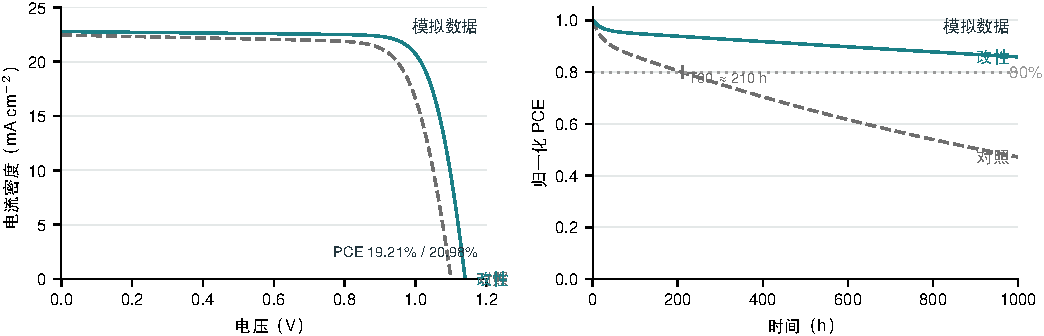
\includegraphics[width=\linewidth]{figures/ch09/ch09-05-data-panels-zh.pdf}
\caption{按最终尺寸（每面板 $84 \times 56\ \text{mm}$）绘制的两个数据面板。(c) 对照（灰色虚线）与改性（青色实线）的模拟 $J\text{--}V$ 曲线。(d) 归一化 PCE 随时间变化，点线为 80\%。两组同时由颜色和线型区分，灰度打印仍可分辨；曲线由单二极管模型与给定衰减函数生成，为模拟教学数据。注意左图右下角：若将直接标注机械绑定在曲线末点，两条在 $V_{\text{oc}}$ 处归零的曲线会导致“对照”“改性”与横轴末位刻度重叠，这一问题在终稿（图~\ref{fig:ch09-07}）中修正。}\label{fig:ch09-05}
\end{figure}

\textbf{第四，用直接标注替代图例框，并排查文字与曲线的几何碰撞。}
在只有两条曲线的数据图中，去掉带边框的图例盒、直接在曲线旁写上同色的“改性”与“对照”，能省去视线在图例与曲线之间来回跳跃的负担。

但直接标注绝不能在脚本里简单写成“把标签放在最后一个数据点 \texttt{(x[-1], y[-1])} 处”。观察图~\ref{fig:ch09-05} 的实际画面，就能看到自动贴末点带来的真实碰撞问题：在左图（面板 \textbf{c}）中，对照与改性两条 $J\text{--}V$ 曲线都在右侧陡降，分别于开路电压 $1.100\ \text{V}$ 和 $1.140\ \text{V}$ 处交于横轴（$J = 0$）。把标签绑在曲线末端，导致“对照”和“改性”两个词在右下角 $1.2\ \text{V}$ 刻度处严重重叠，而右下方的“PCE 19.21\% / 20.98\%”又被灰色虚线直接穿过；在右图（面板 \textbf{d}）中，右端的“改性”“80\%”“对照”紧贴曲线末端，且“$\text{T80} \approx 210\ \text{h}$”压在了虚线上。

这说明\textbf{直接标注必须根据曲线走势人工放置在邻近的空白通带（open band）内，并放大到 200\% 复核}。在终稿（图~\ref{fig:ch09-07}）中，我们将面板 \textbf{c} 的“改性”和“对照”移到陡降段左侧的开阔区（分别为 $(0.96\ \text{V},\ 15.5\ \text{mA cm}^{-2})$ 与 $(1.00\ \text{V},\ 5.0\ \text{mA cm}^{-2})$），把 PCE 汇总移到左下角 $(0.03,\ 0.04)$；将面板 \textbf{d} 的标注移到各自曲线上方的空白带并加半透明白底衬垫，彻底消除了压线与撞字。

\textbf{第五，统一物理量单位与面板内真实性声明。}
删除单图顶部与图注重复的独立标题（如“J-V curve”“Stability test”）；单位格式全图统一为 $\text{V}$、$\text{mA cm}^{-2}$、$\text{h}$，二氧化锡下标用数学模式排为 $\mathrm{SnO_2}$；并在面板内部直接标出“不按比例”（\textbf{a}）、“模型生成示意，非显微图像”（\textbf{b}）和“模拟数据”（\textbf{c}、\textbf{d}），确保单面板被截图放进幻灯片或海报时声明不丢失。

\section{对齐、编号与留白}

将四个面板排入同一张画布时，决定版面是否整洁专业的核心是三件事：对齐、编号与留白。

\textbf{第一件事：对齐坐标轴框（spine box），而不是对齐图片外框（bounding box）。}
面板 \textbf{c} 的纵轴刻度是两位数整数（\texttt{0–25}）且轴标题含括号与上标，面板 \textbf{d} 的纵轴刻度是一位小数（\texttt{0.0–1.0}）。如果把两张开启了自动紧凑裁剪（\texttt{bbox\_inches='tight'}）的单图拖进画布并对齐图片左边缘，由于两图左侧文字宽度不同，里面的坐标轴矩形框反而会一左一右、一高一低。

读者扫视并排图表时，眼睛寻找的基准线是实实在在画出来的坐标轴线。因此，合成组图时不应使用弹性自适应布局（\texttt{tight\_layout}），而应\textbf{以毫米为单位直接固定每个面板框在画布上的绝对矩形坐标}。例如在终稿（图~\ref{fig:ch09-07}）的 $174.0 \times 116.0\ \text{mm}$ 画布上，左起先留 $13.0\ \text{mm}$ 给左列纵轴标题与刻度，左列（面板 \textbf{a} 外框与面板 \textbf{c} 坐标轴框）统一占据 $x = 13.0\text{--}82.0\ \text{mm}$（宽 $69.0\ \text{mm}$）；中间留 $6.0\ \text{mm}$ 列间距和 $13.0\ \text{mm}$ 右列纵轴走廊，右列（面板 \textbf{b} 外框与面板 \textbf{d} 坐标轴框）统一占据 $x = 101.0\text{--}170.0\ \text{mm}$（宽 $69.0\ \text{mm}$），最右侧留 $4.0\ \text{mm}$ 边距并将末位刻度“1.2”与“1000”设为右对齐内收；下排 \textbf{c}、\textbf{d} 坐标轴框底边统一固定在 $y = 11.0\ \text{mm}$、高 $46.0\ \text{mm}$，并用脚本断言（\texttt{assert}）自动校验四框边界坐标完全相等。

\textbf{第二件事：面板字母统一样式、位置与基线，置于画布外侧白底走廊。}
面板编号字母是正文、图注与画面之间的唯一定位路标，必须遵守四条规则：
\begin{enumerate}
\item \textbf{样式全图唯一：}按目标期刊规范统一格式（本例采用 $10\ \text{pt}$ TeX Gyre Heros Bold 粗体无衬线小写 \textbf{a}–\textbf{d}，不加括号和句点）。
\item \textbf{对齐面板左缘与同行基线：}左列字母 \textbf{a}、\textbf{c} 左缘对齐 $x = 13.0\ \text{mm}$，右列字母 \textbf{b}、\textbf{d} 左缘对齐 $x = 101.0\ \text{mm}$；上排 \textbf{a}、\textbf{b} 与下排 \textbf{c}、\textbf{d} 各自共享同一条水平基线（均位于面板框顶边上方 $1.0\ \text{mm}$）。
\item \textbf{顶部预留安全带：}在画布顶部专门留出 $5.0\ \text{mm}$ 白边走廊，防止上排面板上方的字母被裁切。
\item \textbf{不压深色图像内部：}字母一律放在面板框外侧的白底走廊上，避免压在面板 \textbf{b} 顶部的暗黑背景上导致看不清。
\end{enumerate}

\textbf{第三件事：用留白传递分组信息，严守图像面板原始宽高比。}
按照视觉接近性原则，不同功能组之间的留白应大于同组内部：本例同排左右列间距为 $6.0\ \text{mm}$，而上排解释组（\textbf{a}、\textbf{b}）与下排数据组（\textbf{c}、\textbf{d}）之间的行距加大为 $8.0\ \text{mm}$。同时，图像面板绝不能为了填满格子而设置非等比拉伸（\texttt{aspect='auto'}）：在 $69.0\ \text{mm}$ 统一列宽下，面板 \textbf{a}（源像素 $1586 \times 992$）自然高度为 $43.2\ \text{mm}$，面板 \textbf{b}（源像素 $1536 \times 1024$）自然高度为 $46.0\ \text{mm}$；让两面板顶边齐平于 $y = 111.0\ \text{mm}$，面板 \textbf{a} 底部自然留出的 $2.8\ \text{mm}$ 白边刚好安放入射光与“不按比例”标签。

\section{完整案例：钙钛矿 Figure 2 从杂乱到可投稿前稿}

现在把前面四节的原则串起来，完整走一遍平面钙钛矿太阳能电池 Figure 2 从材料准备、任务书、底图生成、初稿排错到终稿复现的全过程（本案例与第 12、13 章共用同一套模拟数据）。

\subsection*{第一步：清点材料与模拟参数}

教学设定比较平面正置（n-i-p）对照器件与界面钝化改性器件。自下而上层序为：玻璃 / FTO / $\text{SnO}_2$（示意厚度约 $30\ \text{nm}$）/ 钙钛矿（约 $500\ \text{nm}$）/ 钝化层（仅改性组，极薄）/ spiro-OMeTAD（约 $200\ \text{nm}$）/ Au（约 $80\ \text{nm}$），光从玻璃侧入射。不指定具体钙钛矿组分与钝化分子，也不报告任何真实器件测试结果。

四项材料中，M1（面板 \textbf{a} 结构示意）和 M2（面板 \textbf{b} 类 SEM 截面图样）由图像模型生成无字底图；M3（面板 \textbf{c} $J\text{--}V$ 曲线）由 Python 脚本按单二极管方程 $J = J_{\text{L}} - J_0[\exp((V + J R_{\text{s}})/(n V_{\text{T}})) - 1] - (V + J R_{\text{s}})/R_{\text{sh}}$ 在 $25\ ^\circ\text{C}$（$V_{\text{T}} = 0.025693\ \text{V}$）、AM1.5G（$100\ \text{mW cm}^{-2}$）下以 $0.5\ \text{mV}$ 步长二分法求解，仅模拟单一扫描方向，不模拟迟滞；M4（面板 \textbf{d} 稳定性曲线，$0\text{--}1000\ \text{h}$，步长 $10\ \text{h}$）按双指数衰减函数 $y(t) = [1 - b(1 - e^{-t/20})]e^{-t/\tau}$ 生成（对照取 $b = 0.08, \tau = 1500\ \text{h}$；改性取 $b = 0.04, \tau = 9000\ \text{h}$）。每组仅有一条代表性模拟曲线，参数与计算指标见表~\ref{tab:ch09-sim}。

\begin{table}[htbp]\centering\footnotesize
\setlength{\tabcolsep}{3.5pt}
\renewcommand{\arraystretch}{1.15}
\caption{面板 c、d 的单二极管模拟参数与计算指标（模拟教学数据）。}\label{tab:ch09-sim}
\begin{tabularx}{\linewidth}{@{}lcccYY@{}}
\toprule
\textbf{组别} & $J_{\text{L}}$ / 目标 $V_{\text{oc}}$ & $n$ & $R_{\text{s}}$ / $R_{\text{sh}}$ ($\Omega\cdot\text{cm}^2$) & \textbf{计算 $J_{\text{sc}}$ / $V_{\text{oc}}$ / FF} & \textbf{计算 PCE 与 $T_{80}$} \\
\midrule
对照 & $22.5\ \text{mA cm}^{-2}$ / $1.10\ \text{V}$ & 1.6 & $2.5$ / $1500$ & $22.46\ \text{mA cm}^{-2}$ / $1.100\ \text{V}$ / $0.777$ & $19.21\%$；$T_{80} = 210\ \text{h}$ \\
改性 & $22.8\ \text{mA cm}^{-2}$ / $1.14\ \text{V}$ & 1.5 & $2.0$ / $3000$ & $22.78\ \text{mA cm}^{-2}$ / $1.140\ \text{V}$ / $0.808$ & $20.98\%$；$T_{80} > 1000\ \text{h}$ \\
\bottomrule
\end{tabularx}
\end{table}

\begin{BookNote}
\textbf{为什么面板 b 不用开放许可的真实 SEM 图？} 公开文献中虽有 CC BY 4.0 许可的真实钙钛矿 SEM 图像，如 Burkitt 等（2018）图 6（使用 Jeol JSM-7800F 拍摄的旋涂与狭缝涂布钙钛矿层俯视 SEM 图，标有 $10\ \mu\text{m}$ 与 $1\ \mu\text{m}$ 比例尺），但该文器件是\textbf{介孔 $\text{TiO}_2$ 支架 + 甲胺铅碘氯钙钛矿、最佳稳定效率约 $7\%$}，与本例平面 $\text{SnO}_2$ 器件和模拟数值毫无关系。若将其放进本例 Figure 2，会让读者误以为形貌和性能来自同一批器件——这正是第 8 章所禁止的“来自不同样品的图像冒充同一来源”。因此本例面板 \textbf{b} 采用模型生成图样并在面板内标注“非显微图像”；真实研究中，面板 \textbf{b} 必须是同批器件的实际 SEM 采集，并按第 8 章保存原图与处理记录。
\end{BookNote}

\subsection*{第二步：组图任务书}

在 \scidraw{} 科研绘图向导（\sdtool{figure-workflow}）中选择“已有图片组图”路线，填写并下载保存完整任务书：

\begin{Prompt}
【用途与读者】论文 Figure 2，双栏通栏 174 mm 宽、高度不超过 120 mm；
读者为钙钛矿光伏方向的同行。目标期刊按 Springer 类要求准备：
文字不小于 8 pt（以期刊现行作者指南为准，投稿前再核对一次）。
【主问题】界面钝化改性是否同时提高了初始效率和运行稳定性？
【面板分工】
a 器件结构（改性器件；钝化层高亮）——回答“改了什么”。
b 截面形貌——回答“各层是否连续、钝化后形貌是否改变”。
  本书为模型生成示意，面板内标注“模型生成示意，非显微图像”。
c J–V 曲线（对照、改性）——回答“初始效率是否提高、提高来自哪个参数”。
d 归一化 PCE 随时间（对照、改性，0.8 参考线）——回答“稳定性是否提高”。
阅读顺序 a->b->c->d：先结构与形貌（是什么），再性能（怎么样）。
【布局】上排 a、b（解释性），下排 c、d（数据）；c、d 坐标轴框上下对齐、
高度相同；面板间距 6 mm；面板字母左上角，粗体小写，同一基线。
【统一规范】全图一种无衬线字体；刻度、轴标题、标注 8 pt，面板字母 10 pt 粗体；
轴线 0.6 pt，数据线 1.2 pt；对照 #6E6E6E 虚线，改性 #1B7F86 实线，
示意图中钝化层也用 #1B7F86；0.8 参考线为浅灰点线；直接标注，不用图例框；
单位写作 V、mA cm^-2、h。
【不可改变】c、d 的全部数值来自 sim-perovskite 数据文件；
b 的宽高比保持原样，不拉伸；c、d 面板内写“模拟数据”；a 写“不按比例”。
【交付】矢量 PDF（文字可选中）+ 600 dpi TIFF；处理记录；图注（作者补全版）。
【验收】在 174 mm 实际尺寸打印或 100% 缩放下：最小文字 >= 8 pt；
c、d 轴框对齐；四个面板字母样式一致；灰度打印能区分两组；
b 未变形；所有“模拟/模型生成/不按比例”标注在面板内可见。
\end{Prompt}

\subsection*{第三步：生成面板 a、b 底图并核查实际偏差}

面板 \textbf{a} 底图使用以下英文提示词生成（底图不含文字，右侧留出 35\% 空白供后期叠加层名）：

\begin{Prompt}
A clean, flat, two-dimensional scientific schematic of a planar thin-film solar
cell shown as a stack of horizontal layers in side view with a slight sense of
thickness. From bottom to top: a thick pale blue-grey translucent glass slab;
a thin light grey conductive layer; a very thin off-white layer; a thicker
dark reddish-brown absorber layer; an extremely thin teal layer (hex #1B7F86)
directly on top of the absorber; a pale yellow layer; and a thin gold metal
layer on top. Three simple upward-pointing light arrows below the glass,
pale yellow with grey outline. The stack occupies the left 65% of the canvas;
leave the right 35% empty white space for labels added later.
White background, vector illustration style, no gradients, no shadows,
no 3D rendering, no glow, no texture. Layers are not to scale but each layer is
clearly separated by a thin dark grey outline.
Absolutely no text, no letters, no numbers, no labels, no symbols, no scale bar.
Aspect ratio 16:10.
\end{Prompt}

将同一提示词连续生成三次（均为 $1586 \times 992\ \text{px}$，宽高比约 $1.599:1$，相对 $16:10$ 偏差 $-0.08\%$）。三次生成均正确呈现了自下而上的七层堆叠、玻璃下方三支向上的浅黄箭头以及干净无字的白底。但三次候选在细节上各有差异：第 2 次生成的青色钝化层偏厚（约 $29\ \text{px}$），弱化了“极薄界面层”的特征；第 3 次的青色偏亮（中值 \texttt{\#298F97}），且右侧空白占到了约 38.5\%。第 1 次生成右侧留白恰占约 35\%，青色层极薄且清晰，实测颜色中值 \texttt{\#20868D} 与目标色 \texttt{\#1B7F86} 三个通道仅差 $5\text{--}7$，故选作主图。同时核查可见主图仍有两处残余偏差：层内有轻微明暗渐变与细颗粒，未严格满足无渐变无纹理；正面玻璃层厚约 $148\ \text{px}$，略薄于钙钛矿层（约 $158\ \text{px}$）。我们在右侧空白处用引线叠加七层名称，并在右下角标明“不按比例”（图~\ref{fig:ch09-03}）。

\begin{figure}[htbp]\centering
\begin{tikzpicture}
\node[anchor=south west,inner sep=0] (img) at (0,0) {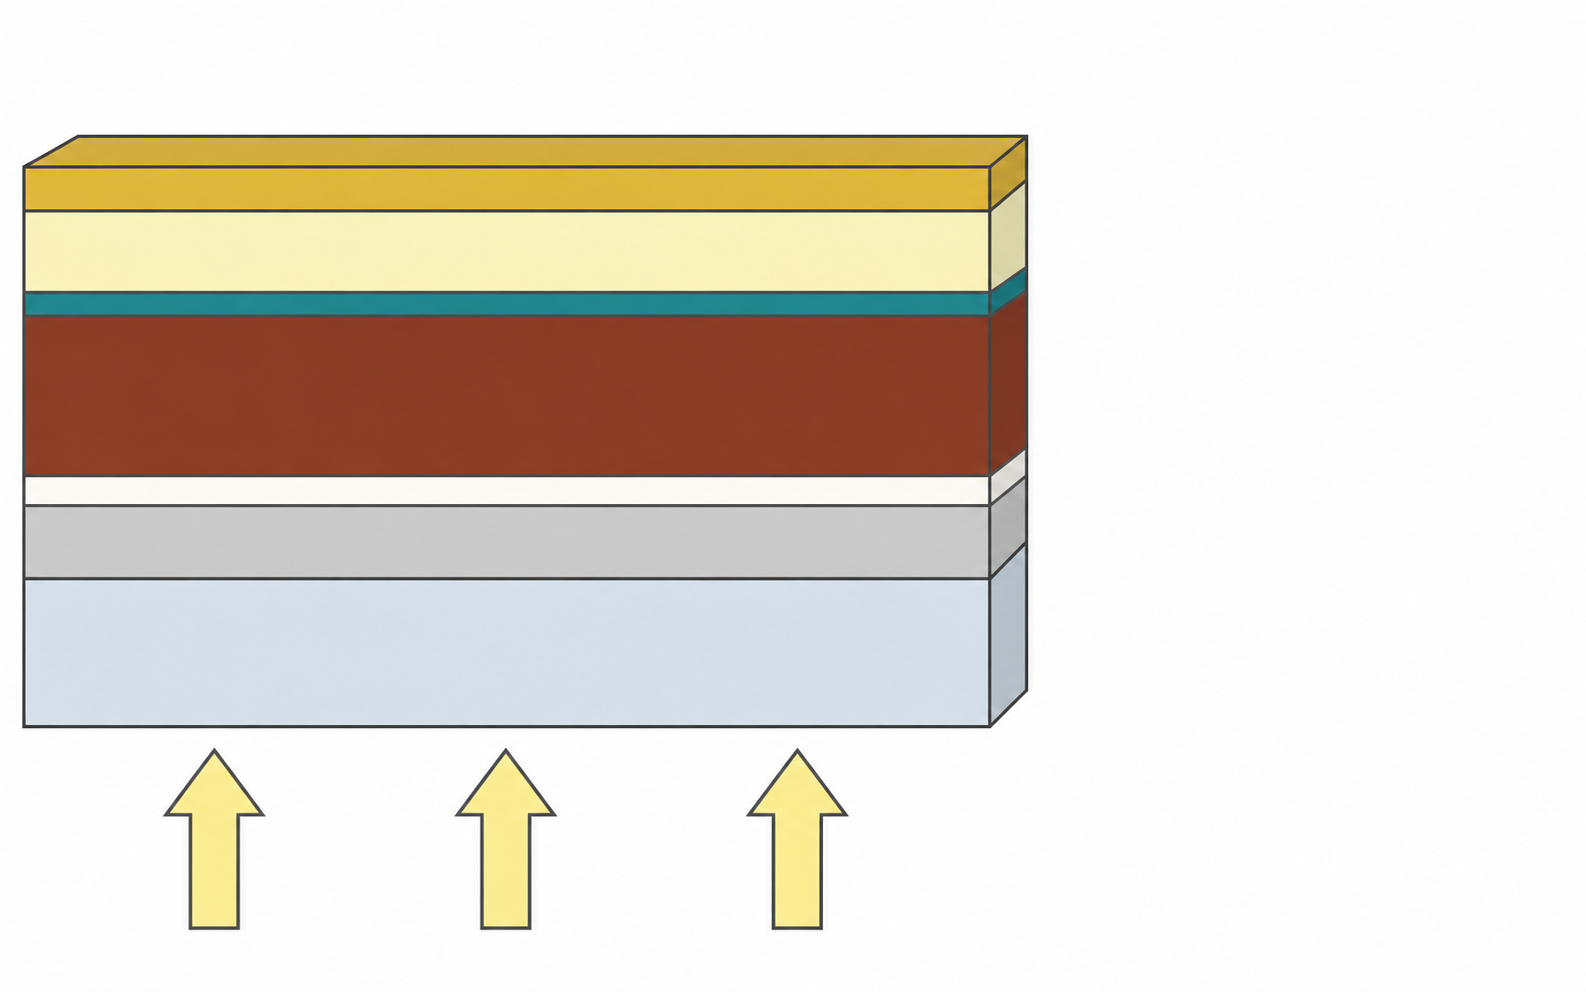
\includegraphics[width=0.86\linewidth]{figures/ch09/ch09-03-device-structure-base.png}};
\begin{scope}[x={(img.south east)},y={(img.north west)},font=\sffamily\footnotesize]
  \draw[BookInk!65,thin] (0.60,0.83) -- (0.69,0.86);
  \draw[BookInk!65,thin] (0.60,0.75) -- (0.69,0.76);
  \draw[BookTeal,thin] (0.60,0.698) -- (0.69,0.67);
  \draw[BookInk!65,thin] (0.60,0.60) -- (0.69,0.56);
  \draw[BookInk!65,thin] (0.60,0.505) -- (0.69,0.45);
  \draw[BookInk!65,thin] (0.60,0.45) -- (0.69,0.39);
  \draw[BookInk!65,thin] (0.60,0.33) -- (0.69,0.25);
  \node[anchor=west] at (0.70,0.86) {Au};
  \node[anchor=west] at (0.70,0.76) {spiro-OMeTAD};
  \node[anchor=west,text=BookTeal,font=\sffamily\footnotesize\bfseries] at (0.70,0.67) {钝化层};
  \node[anchor=west] at (0.70,0.56) {钙钛矿};
  \node[anchor=west] at (0.70,0.45) {$\mathrm{SnO_2}$};
  \node[anchor=west] at (0.70,0.39) {FTO};
  \node[anchor=west] at (0.70,0.25) {玻璃};
  \node[anchor=west] at (0.30,0.05) {入射光};
  \node[anchor=south east,text=BookInk!80] at (0.98,0.02) {不按比例};
\end{scope}
\end{tikzpicture}
\caption{改性器件结构示意（面板 a 底图由图像生成模型绘制，层名为后加标签）。钝化层与数据图中的“改性”使用同一青色。各层厚度不按比例。}\label{fig:ch09-03}
\end{figure}

面板 \textbf{b} 底图使用以下英文提示词生成（刻意禁止比例尺与仪器数据条，因为模型生成图样没有物理尺度）：

\begin{Prompt}
A grayscale illustration in the visual style of a cross-sectional scanning
electron micrograph of a layered thin film, for use as a clearly labelled
teaching illustration. From bottom to top: a thick smooth featureless layer
filling the bottom third; a very thin slightly brighter layer; a thicker layer
made of densely packed columnar grains with visible grain boundaries; a
smoother amorphous layer; and a thin bright layer at the top. Dark background
above the top layer. Slightly irregular fractured edge. Even illumination,
moderate contrast. No scale bar, no data bar, no measurement marks, no text,
no letters, no numbers, no labels, no watermark. Aspect ratio 3:2.
\end{Prompt}

三次生成均为 $1536 \times 1024\ \text{px}$（严格 $3:2$），五个视觉层序清楚且无伪文字或伪比例尺。第 1 次生成的柱状晶粒间裂隙过深；第 2 次底层占比扩大到 $42\%\text{--}43\%$ 且顶部右端有明显下折斜坡；第 3 次（选作主图）顶部断面起伏自然、晶界清晰，但底层仍占整幅高度约 $38\%\text{--}39\%$（略高于提示词要求的下三分之一）且带细微颗粒感，RGB 三通道也并非逐像素严格相等（单像素最大通道差为 $10$）。我们在画面左下角叠加白底黑字声明框“模型生成示意，非显微图像”（图~\ref{fig:ch09-04}）。

\begin{figure}[htbp]\centering
\begin{tikzpicture}
\node[anchor=south west,inner sep=0] (img) at (0,0) {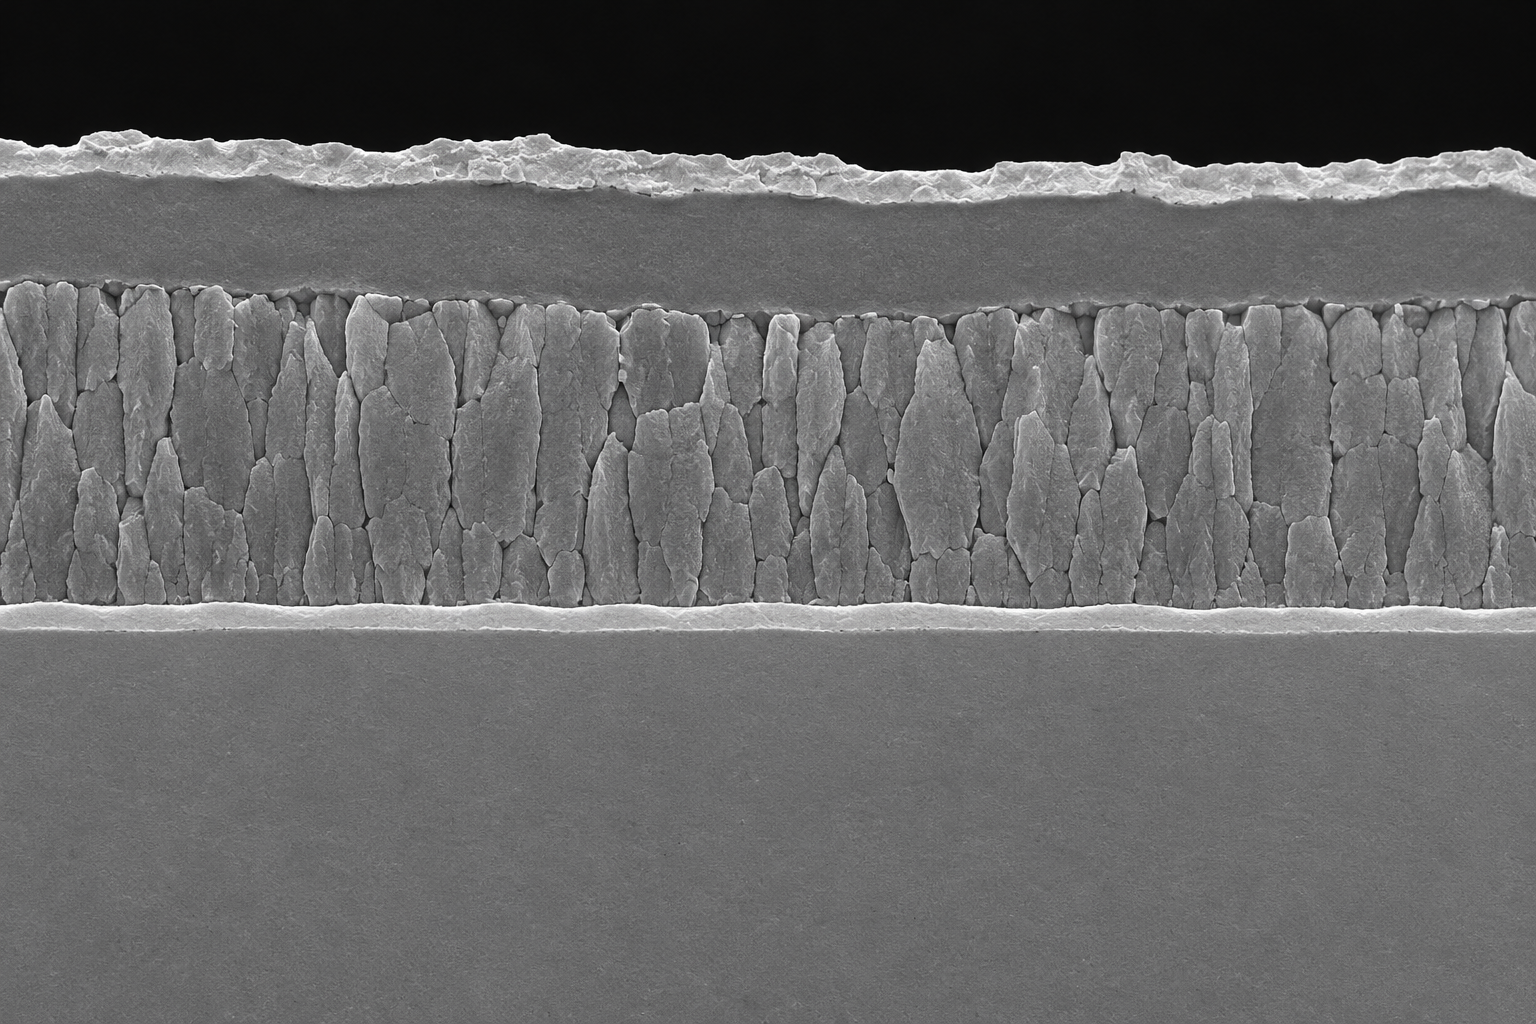
\includegraphics[width=0.78\linewidth]{figures/ch09/ch09-04-sem-like-illustration-base.png}};
\begin{scope}[x={(img.south east)},y={(img.north west)}]
  \node[anchor=south west,fill=white,fill opacity=0.90,text opacity=1,text=black,font=\sffamily\footnotesize,inner sep=2.5pt] at (0.02,0.03) {模型生成示意，非显微图像};
\end{scope}
\end{tikzpicture}
\caption{截面形貌的模型生成示意（面板 b）。本图由图像生成模型绘制，不是显微图像，没有物理比例尺，仅用于示意层序与版式。真实论文中此面板必须是同批器件的实际 SEM 图像，并保留原图与处理记录（见第 8 章）。}\label{fig:ch09-04}
\end{figure}

\subsection*{第四步：初次拼合（v1）的十个问题与修改单}

图~\ref{fig:ch09-06} 复现了“各面板分别做好后直接拖进同一画布”的初稿（v1），红底编号 1–10 标出了画面上的十处具体问题：

\begin{figure}[htbp]\centering
\begin{tikzpicture}
\definecolor{ChNineBad}{HTML}{C0392B}
\node[anchor=south west,inner sep=0] (img) at (0,0) {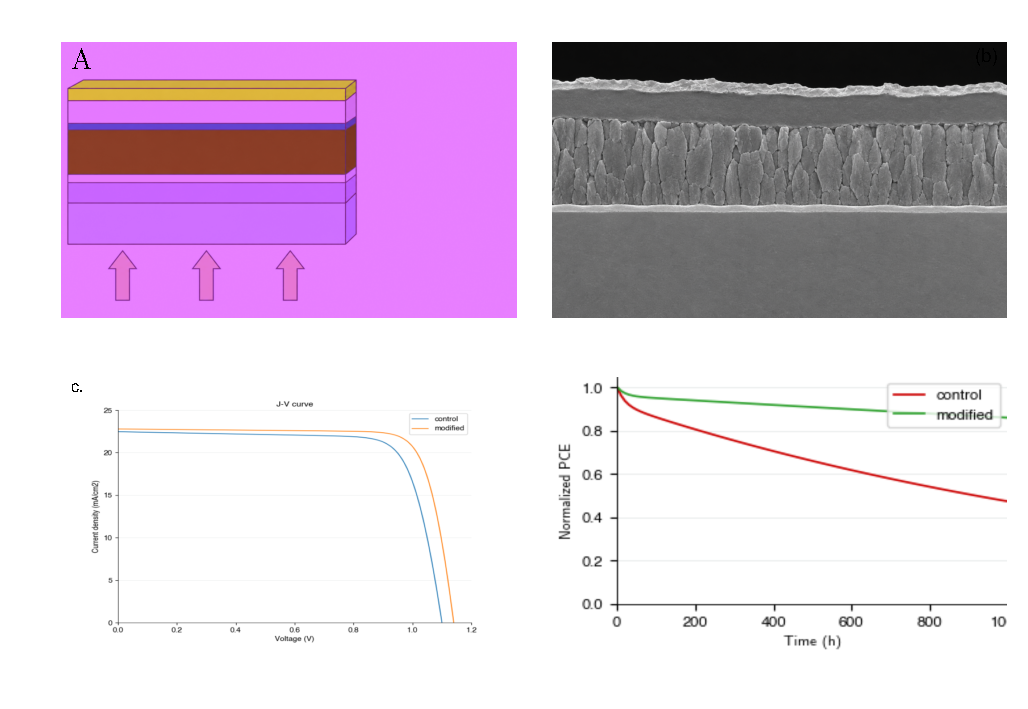
\includegraphics[width=\linewidth]{figures/ch09/ch09-06-assembly-v1-zh.pdf}};
\begin{scope}[x={(img.south east)},y={(img.north west)}]
  \tikzset{
    badnum/.style={draw=white,line width=0.7pt,fill=ChNineBad,text=white,circle,font=\sffamily\bfseries\scriptsize,inner sep=1pt,minimum size=4.0mm},
    badtxt/.style={fill=white,fill opacity=0.88,text opacity=1,text=ChNineBad!90!black,font=\sffamily\scriptsize\bfseries,inner sep=1.2pt,rounded corners=1pt}
  }
  \node[badnum] (b1) at (0.03,0.95) {1};
  \node[badtxt,anchor=west] at (b1.east) {面板字母混用};
  \node[badnum] (b2) at (0.62,0.30) {2};
  \node[badtxt,anchor=west] at (b2.east) {字号不一};
  \node[badnum] (b3) at (0.20,0.70) {3};
  \node[badtxt,anchor=west] at (b3.east) {颜色语义不一致};
  \node[badnum] (b4) at (0.85,0.20) {4};
  \node[badtxt,anchor=east] at (b4.west) {灰度不可分};
  \node[badnum] (b5) at (0.75,0.40) {5};
  \node[badtxt,anchor=west] at (b5.east) {图例压线};
  \node[badnum] (b6) at (0.50,0.08) {6};
  \node[badtxt,anchor=west] at (b6.east) {轴框未对齐};
  \node[badnum] (b7) at (0.75,0.75) {7};
  \node[badtxt,anchor=west] at (b7.east) {b 被拉伸};
  \node[badnum] (b8) at (0.50,0.52) {8};
  \node[badtxt,anchor=west] at (b8.east) {间距不一};
  \node[badnum] (b9) at (0.92,0.92) {9};
  \node[badtxt,anchor=east] at (b9.west) {缺少模拟/模型生成标注};
  \node[badnum] (b10) at (0.30,0.45) {10};
  \node[badtxt,anchor=west] at (b10.east) {面板标题重复图注};
\end{scope}
\end{tikzpicture}
\caption{初次拼合（v1，刻意复现的反例）。编号 1–10 为正文讨论的问题。b 为模型生成示意，非显微图像；c、d 为模拟数据——本版缺少这些面板内标注，正是问题 9。}\label{fig:ch09-06}
\end{figure}

\begin{enumerate}
\item \textbf{面板字母混用且漏标（1）：}a 处为 $14\ \text{pt}$ 衬线大写“A”，b 处为右上角深黑背景中几乎不可见的 $9\ \text{pt}$“(b)”，c 处为“c.”，d 漏标字母。
\item \textbf{字号相差近一倍（2）：}c 按 $8 \times 6\ \text{in}$ 默认尺寸出图后缩入格子，刻度仅约 $4.5\ \text{pt}$；d 按 $84 \times 56\ \text{mm}$、$8\ \text{pt}$ 出图，且右端刻度“1000”被画布边裁成“10”。
\item \textbf{颜色语义不一致（3）：}a 因色相偏移使钝化层变深紫、白底染紫红；c 用默认蓝/橙；d 用红/绿，同一组在三处颜色完全不同。
\item \textbf{灰度不可分（4）：}c、d 两组均为实线，且 d 的红/绿撞色对色觉异常读者不友好。
\item \textbf{图例框压线（5）：}c、d 带边框图例，其中 d 的图例框直接压在绿色改性曲线上。
\item \textbf{坐标轴框未对齐（6）：}c 与 d 的坐标轴左缘错位约 $1.4\ \text{mm}$，底边错位约 $3.2\ \text{mm}$。
\item \textbf{图像被拉伸（7）：}b 以 \texttt{aspect='auto'} 拉伸到与 a 同高，晶粒形貌纵向失真。
\item \textbf{面板间距不一（8）：}网格留白不均，缺少“组间大于组内”的分组层次。
\item \textbf{缺少面板内声明与参考线（9）：}无“模拟数据”“模型生成示意”“不按比例”标注，a 无层名，d 缺 $0.8$ 参考线。
\item \textbf{面板标题重复图注且单位不规范（10）：}c、d 顶部带“J-V curve”“Stability test”标题，c 纵轴单位写成 \texttt{mA/cm2}。
\end{enumerate}

针对这十个问题，逐条开具修改单：

\begin{Prompt}
修改单
1. 面板字母统一为粗体小写 a–d，10 pt，位于各面板左上角外侧，同一基线（画布顶留 5 mm）。
2. c、d 按最终尺寸在 174 × 116 mm 画布上直接重绘，所有文字 8 pt，拼合缩放系数为 1.0。
3. 颜色语义统一：对照 #6E6E6E 虚线，改性 #1B7F86 实线；a 恢复白底原图，钝化层标签用 #1B7F86。
4. 去掉图例框，在曲线内侧空白带直接标注“对照”“改性”（字号 8 pt，颜色同曲线）。
5. 固定四面板左右缘：左列 a、c 为 x = 13–82 mm，右列 b、d 为 x = 101–170 mm；
   c、d 轴框底边均为 y = 11 mm、高 46 mm；末位刻度“1.2”与“1000”右对齐内收。
6. a、b 按原始宽高比置入（宽 69 mm，高 43.2 mm 与 46.0 mm），顶边齐平，不拉伸。
7. 列间距统一 6 mm（另留 13 mm 纵轴走廊）；上下排之间留 8 mm 行距。
8. c、d 右上角加“模拟数据”；b 左下角加“模型生成示意，非显微图像”；
   a 加层名与右下角“不按比例”；d 加 0.8 点线参考线并标“80%”与“T80 约 210 h”。
9. 删除面板内标题；单位统一为 V、mA cm^-2、h。
10. 导出矢量 PDF（pdf.fonttype 42）与 300 dpi PNG；记录每个面板的尺寸与缩放系数。
\end{Prompt}

\subsection*{第五步：修订终稿（v2）与 SciDraw AI 组图工具复现}

按修改单生成的修订版（v2）见图~\ref{fig:ch09-07}。若使用 \scidraw{} 组图工具（\sdtool{multi-panel-figure-maker}）排版同一张图，操作与核对要点如下：

\begin{figure}[htbp]\centering
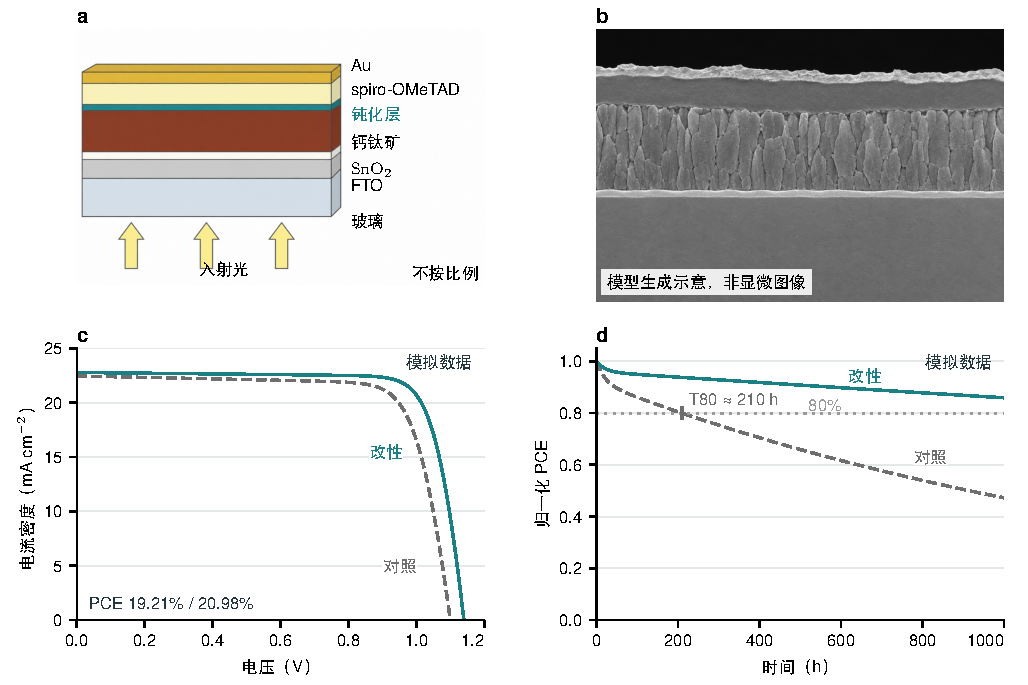
\includegraphics[width=\linewidth]{figures/ch09/ch09-07-assembly-final-zh.pdf}
\caption{修订后的组图（v2）。\textbf{图 2 | 界面钝化对钙钛矿太阳能电池初始性能与运行稳定性的影响（模拟教学数据）。} \textbf{a}，改性器件结构示意（玻璃/FTO/$\text{SnO}_2$/钙钛矿/钝化层/spiro-OMeTAD/Au，光从玻璃侧入射）；对照器件无钝化层；各层厚度不按比例。\textbf{b}，截面形貌示意，由图像生成模型绘制，\textbf{非显微图像}，仅示意层序。\textbf{c}，对照（灰色虚线）与改性（青色实线）器件的 $J\text{--}V$ 曲线，按单二极管模型模拟（AM1.5G，$100\ \text{mW cm}^{-2}$，单一扫描方向，未模拟迟滞）；对照 PCE 19.21\%，改性 20.98\%。\textbf{d}，归一化 PCE 随时间的变化（模拟条件：连续 1 个太阳光照、最大功率点跟踪、氮气、约 $25\ ^\circ\text{C}$）；点线为初始值的 80\%，对照 $T_{80}$ 约 $210\ \text{h}$，改性在 $1000\ \text{h}$ 内未降至 80\%。c、d 每组为一条模拟曲线，不代表器件间分布，未做统计检验。模拟参数与脚本见本书仓库。}\label{fig:ch09-07}
\end{figure}

\begin{enumerate}
\item \textbf{文件交接与期刊预设：}工具间不自动传图，需先将已叠好标签的 \textbf{a}、\textbf{b} PNG 和按终尺寸导出的 \textbf{c}、\textbf{d} PNG 上传至 \texttt{/multi-panel-\allowbreak figure-\allowbreak maker}（当前文档保存在浏览器本地存储中）。选择 Springer 或 Cell 的双栏 $174\ \text{mm}$ 预设与 $2 \times 2$ 网格，开启自动编号。注意编号样式跟随期刊预设（Springer 预设为小写 \textbf{a}，Cell 预设为大写 \textbf{A}），投稿前须对照作者指南核实。
\item \textbf{导出格式与能力边界：}导出包含 TIFF、PNG、PDF、PPTX 与处理记录的 ZIP 包。PPTX 中面板位图与编号文字可分别编辑，但面板内部文字不可编辑；组图工具不提供 AI 自动规划布局、修改面板内文字或将位图转为可编辑矢量，这些必须在生成单面板时解决。
\item \textbf{读处理记录核算实际字号与有效分辨率：}处理记录给出各面板在图中的毫米尺寸和缩放系数。若面板 \textbf{c} 原图按 $84\ \text{mm}$ 宽、$8\ \text{pt}$ 出图，但在组图中被放成 $80\ \text{mm}$ 宽（缩放系数 $80/84 \approx 0.952$），实际字号 $= 8 \times 80 / 84 \approx 7.6\ \text{pt}$，就低于 $8\ \text{pt}$ 要求；正确做法是回到脚本按格子实际尺寸重出，而不是在组图工具里放大。位图有效分辨率按“源像素宽 $\div$ 印刷英寸宽”计算：在图~\ref{fig:ch09-07} 中，面板 \textbf{a}（$1586\ \text{px}$）与面板 \textbf{b}（$1536\ \text{px}$）在 $69.0\ \text{mm}$（$2.717\ \text{in}$）宽下的有效分辨率分别为 $1586 / 2.717 \approx 584\ \text{ppi}$ 与 $1536 / 2.717 \approx 565\ \text{ppi}$，均远高于 $300\ \text{ppi}$ 的常规要求。
\end{enumerate}

\section{图注：AI 起草，作者补全}

一段完整的组图图注包含五个构件：总标题句、逐面板说明（含视觉编码定义）、关键实验或模拟条件、样本量与统计方法、数据性质与来源声明。

把终稿 PNG 上传至 \scidraw{} 图注辅助工具（\sdtool{figure-legend}）并选择输出语言后，工具只看图片像素，输出一段 40–120 词的描述性图注草稿。例如预期草稿形态通常为：“钙钛矿太阳能电池的器件结构、截面形貌与光伏性能。(a) 器件层状结构示意。(b) 器件截面图像。(c) 对照与改性器件的 J–V 曲线。(d) 归一化 PCE 随时间的变化。”

按设计原则，\sdtool{figure-legend} 绝不编造画面中看不到的样本量、$p$ 值、统计检验、处理条件或化学分子式。作者拿到草稿后，必须把“看图可见的”与“必须知道的”分开核对（图~\ref{fig:ch09-08}）：

\begin{figure}[htbp]\centering
\resizebox{\linewidth}{!}{% FIG ch09-08 legend drafting (Chinese)
\begin{tikzpicture}[
  x=1mm, y=1mm,
  font=\sffamily\scriptsize,
  text=BookInk,
  col/.style={draw=BookInk!45, line width=0.4pt, rounded corners=1pt, inner sep=2mm, align=justify, text width=78mm},
  hi/.style={fill=BookPale, draw=BookTeal, line width=0.8pt, rounded corners=1pt, inner sep=1.5mm},
  tag/.style={font=\tiny\bfseries, text=BookTeal, anchor=east},
]
  \node[font=\small\bfseries, anchor=west] at (0, 118) {图注起草对照};
  \node[col, anchor=north west] (draft) at (0, 112) {
    \textbf{/figure-legend 草稿（实测原文）}\par\vspace{1mm}
    \fbox{\parbox[t]{72mm}{\centering 待实测，见 \texttt{provenance/ch09/figure-legend-draft-zh.txt}}}
  };
  \node[col, anchor=north west] (final) at (88, 112) {
    \textbf{作者补全版（节选）}\par\vspace{1mm}
    \tikz{\node[hi, text width=72mm, anchor=west] (t1) at (0,0) {
      \textbf{图 2 |} 界面钝化对钙钛矿太阳能电池初始性能与运行稳定性的影响（\textbf{模拟教学数据}）。
    }; \node[tag] at (-1,0) {【数据性质】};}\par
    \tikz{\node[hi, text width=72mm, anchor=west] (t2) at (0,0) {
      \textbf{b}，截面形貌示意，由图像生成模型绘制，\textbf{非显微图像}……
    }; \node[tag] at (-1,0) {【定义】};}\par
    \tikz{\node[hi, text width=72mm, anchor=west] at (0,0) {
      c、d 每组为一条模拟曲线，未做统计检验；脚本见 \texttt{sim\_perovskite.py}。
    }; \node[tag] at (-1,0) {【来源】};}
  };
  \node[anchor=west, text=BookInk!70] at (0, 4) {
    删改示例：\sout{截面图像} $\rightarrow$ 模型生成示意，非显微图像
  };
\end{tikzpicture}
}
\caption{图注由 AI 起草、作者补全。左：\sdtool{figure-legend} 根据图像生成的草稿框；右：作者补全版，高亮部分是图像中看不到、必须由作者提供的信息。}\label{fig:ch09-08}
\end{figure}

\begin{itemize}
\item \textbf{删改视觉误判：}草稿可能把面板 \textbf{b} 写成“截面图像/SEM 图像”，必须改为“截面形貌示意，由图像生成模型绘制，非显微图像，仅示意层序”。
\item \textbf{补齐五类背景信息：}(1) \textbf{【数据性质】}模拟教学数据、各层厚度不按比例、非显微图像；(2) \textbf{【器件与条件】}七层结构与光入射方向、单二极管模型（AM1.5G，$100\ \text{mW cm}^{-2}$，单一扫描方向，未模拟迟滞——真实钙钛矿电池存在反常迟滞，须按 Snaith 等 2014 报告扫描方向与速率）、连续 1 个太阳光照、最大功率点跟踪、氮气、约 $25\ ^\circ\text{C}$（若标注 ISOS-L-1 等标准代号，须对照 Khenkin 等 2020 核实全部测试条件）；(3) \textbf{【样本与统计】}对照 PCE $19.21\%$、改性 $20.98\%$，声明每组一条模拟曲线、不代表器件间分布、未做统计检验；(4) \textbf{【定义】}点线为初始值的 80\%，对照 $T_{80}$ 约 $210\ \text{h}$，改性在 $1000\ \text{h}$ 内未降至 80\%；(5) \textbf{【来源】}模拟参数与脚本位置（完整终稿图注见图~\ref{fig:ch09-07}）。
\end{itemize}

在真实实验论文中，作者可按如下填空模板补齐样本量与统计信息（\texttt{【】}内由作者据实验记录填入）：

\begin{BookNote}
\textbf{真实论文版图注模板：} \textbf{c}，……代表性器件的 $J\text{--}V$ 曲线（反向扫描，【扫描速率】$\text{mV s}^{-1}$，【有效面积】$\text{cm}^2$，掩膜【有/无】）；插表为 $n =$【器件数】个器件、来自【批次数】个独立批次的光伏参数（均值 $\pm$ 标准差）。\textbf{d}，……$n =$【器件数】个未封装器件，【气氛】，【温度】$^\circ\text{C}$，阴影为【标准差/标准误/范围】；$T_{80}$ 定义为【首次降至初始值 80\% 的时间/拟合值】。统计检验：【检验方法】，【$P$ 值】。
\end{BookNote}

交付前，结合 \sdtool{figure-checker} 与脚本断言完成八项终审核验（表~\ref{tab:ch09-verify}）。

\begin{table}[htbp]\centering\footnotesize
\setlength{\tabcolsep}{3pt}
\renewcommand{\arraystretch}{1.15}
\caption{本章案例终稿（图~\ref{fig:ch09-07}）的八项交付前核验。}\label{tab:ch09-verify}
\begin{tabularx}{\linewidth}{@{}>{\raggedright\arraybackslash}p{26mm}YY@{}}
\toprule
\textbf{核验项} & \textbf{检查方法} & \textbf{终稿实测结果} \\
\midrule
数值一致性 & 脚本断言比对数据表与图面、图注数字 & PCE $19.21\%$/$20.98\%$、$T_{80}=210\ \text{h}$/$>1000\ \text{h}$ 完全一致 \\
100\% 缩放字号 & 在 $174\ \text{mm}$ 宽下查 PDF 字体属性或量大写字母高（$8\ \text{pt} \approx 2.0\ \text{mm}$） & 面板字母 $10\ \text{pt}$ 粗体，其余文字均 $8\ \text{pt}$，无越界裁切 \\
坐标轴框对齐 & 检验四框毫米坐标（\texttt{ax.get\_position()} 断言） & a/c 对齐 $13\text{--}82\ \text{mm}$，b/d 对齐 $101\text{--}170\ \text{mm}$，c/d 底边均 $11\ \text{mm}$ \\
图像宽高比 & 对比置入框与原图宽高比 & a（$69.0 \times 43.2\ \text{mm}$）、b（$69.0 \times 46.0\ \text{mm}$）误差 $< 0.1\%$ \\
灰度与色觉 & 灰度转换及 Machado（2009）色觉模拟 / \sdtool{figure-checker} & 灰虚线、青实线与浅灰点线在灰度与色觉模拟下均可区分 \\
面板内声明 & 目视检查四面板内部声明文字 & “不按比例”“模型生成示意，非显微图像”“模拟数据”均清晰可见 \\
缩放系数与 ppi & 查处理记录缩放系数，算源像素 $\div$ 印刷英寸宽 & c、d 缩放系数 $1.0$；a 约 $584\ \text{ppi}$、b 约 $565\ \text{ppi}$ \\
图注可溯源 & 逐项核对图注数字与说明出处 & 全部来自数据文件与脚本设定，无图中不可见且无依据的内容 \\
\bottomrule
\end{tabularx}
\end{table}

\section{AI 在这一步能做什么与不能做什么}

组图与图注各环节中 AI、确定性工具与作者的职责边界汇总于表~\ref{tab:ch09-01}。

\begin{table}[htbp]\centering\footnotesize
\setlength{\tabcolsep}{3pt}
\renewcommand{\arraystretch}{1.15}
\caption{AI 在组图环节能做、不能做与作者要核对的内容。}\label{tab:ch09-01}
\begin{tabularx}{\linewidth}{@{}>{\raggedright\arraybackslash}p{18mm}YYY@{}}
\toprule
\textbf{环节} & \textbf{AI 能做} & \textbf{AI 不能做} & \textbf{作者要核对} \\
\midrule
面板分工 & 根据任务书列出面板分工与顺序候选；指出与主问题无关的面板 & 判断证据是否足以支持结论；决定哪些数据可以不放 & 每个面板回答的子问题；被移出的面板去向（补充材料） \\
网格规划 & 按期刊宽度换算格子尺寸；写 \texttt{gridspec} / 固定轴框的脚本 & 理解面板内容的科学重要性来分配面积（当前组图工具不做 AI 布局规划） & 最终尺寸、宽高比不变、分组留白 \\
示意面板 & 生成无字底图（结构、层序、示意形貌） & 保证层序、比例与真实器件一致；生成可作证据的形貌图 & 层数与顺序；颜色语义；“示意/模型生成”标注 \\
数据面板 & 按规范写绘图脚本；统一 \texttt{rcParams} & 选择或修改数据；补出没有的误差带 & 数值来自数据文件；字号在最终尺寸下达标；灰度可分 \\
排版与导出 & \scidraw{} 组图工具：网格、跨行列、自动编号、期刊尺寸预设、处理记录、TIFF/PNG/PDF/PPTX & 修改面板内部文字；统一已经栅格化的面板字体；把位图变成可编辑矢量 & 处理记录中的缩放系数与有效分辨率；编号样式符合期刊 \\
图注 & \sdtool{figure-legend} 起草看图可见的描述 & 写样本量、批次、测试条件、统计方法、数据性质（工具按设计不编造） & 补全 $n$、条件、统计、定义、来源；删去误判（如把示意写成 SEM） \\
技术检查 & \sdtool{figure-checker} 检查格式、分辨率、灰度与色觉风险 & 审核科学结论或统计选择 & 检查报告之外的科学核验 \\
\bottomrule
\end{tabularx}
\end{table}

\section{本章检查清单}

\begin{itemize}
\item 写下了组图的主问题，每个面板都有明确的子问题或证据角色；无关面板已移出。
\item 画布按目标期刊最终宽度（本例 $174\ \text{mm}$）设定，高度在限制内。
\item 数据面板按最终格子尺寸出图，拼合时缩放系数为 $1.0$（或已据此换算实际字号）。
\item 全图一种字体；最小字号满足期刊要求；面板字母样式、大小、位置统一。
\item 同组数据面板的坐标轴框对齐；面板间距一致，组间留白大于组内。
\item 同一组别在所有面板中颜色相同；颜色之外还有线型或标注区分；灰度与色觉模拟通过。
\item 图像面板保持原宽高比，没有拉伸。
\item 模拟数据、模型生成图样、不按比例等声明写在\textbf{面板内}，也写在图注中。
\item 图注包含：标题句、逐面板说明、样本量与重复、测试条件、统计方法与误差含义、定义（如 $T_{80}$）、数据与代码来源。
\item 处理记录、脚本、原始数据与组图导出文件一并保存；从数据脚本到组图工具的文件交接有记录。
\end{itemize}

\section{练习}

\begin{enumerate}
\item \textbf{面板分工（纸笔）。} 取你最近的一张论文组图，写出它的主问题和每个面板的子问题；找出一个不直接回答主问题的面板，说明它应该留下、合并还是移到补充材料。
\item \textbf{最终尺寸检查（脚本）。} 用本章配套的数据面板绘图脚本把面板 \textbf{c} 分别按 $\text{figsize}=(8,6)\ \text{in}$ 和 $84 \times 56\ \text{mm}$ 出图，都放进 $84\ \text{mm}$ 宽的格子里，计算两种情况下刻度文字的实际字号；再把对照曲线改为与改性同为实线，转灰度，记录能否区分。
\item \textbf{\scidraw{} 实操。} 把本章提供的四个面板 PNG 导入 \texttt{/multi-panel-\allowbreak figure-\allowbreak maker}，分别选 Springer 与 Cell 的 $174\ \text{mm}$ 预设，比较编号样式的差别；导出 ZIP，从处理记录中读出 \textbf{c} 的缩放系数并换算实际字号。然后把导出的 PNG 上传 \sdtool{figure-legend}，保存草稿原文，按第 9.6 节的类别逐项补全图注。附加：阅读 Burkitt 等（2018）图 6（CC BY 4.0，真实 SEM 图），列出一张真实 SEM 面板在图中和图注里分别需要提供的信息（仪器、视角、比例尺、样品与工艺），并说明为什么不能把它放进本章的 Figure 2。
\end{enumerate}

\section*{参考文献}

\begin{itemize}
\item Burkitt D, Searle J, Watson T. Perovskite solar cells in N-I-P structure with four slot-die-coated layers. \textit{Royal Society Open Science}. 2018;5(5):172158. doi:10.1098/rsos.172158
\item Crameri F, Shephard GE, Heron PJ. The misuse of colour in science communication. \textit{Nature Communications}. 2020;11:5444. doi:10.1038/s41467-020-19160-7
\item Jambor H, Antonietti A, Alicea B, et al. Creating clear and informative image-based figures for scientific publications. \textit{PLOS Biology}. 2021;19(3):e3001161. doi:10.1371/journal.pbio.3001161
\item Khenkin MV, Katz EA, Abate A, et al. Consensus statement for stability assessment and reporting for perovskite photovoltaics based on ISOS procedures. \textit{Nature Energy}. 2020;5(1):35--49. doi:10.1038/s41560-019-0529-5
\item Kojima A, Teshima K, Shirai Y, Miyasaka T. Organometal halide perovskites as visible-light sensitizers for photovoltaic cells. \textit{Journal of the American Chemical Society}. 2009;131(17):6050--6051. doi:10.1021/ja809598r
\item Machado GM, Oliveira MM, Fernandes LAF. A physiologically-based model for simulation of color vision deficiency. \textit{IEEE Transactions on Visualization and Computer Graphics}. 2009;15(6):1291--1298. doi:10.1109/TVCG.2009.113
\item Nature Portfolio. Preparing figures -- our specifications. \url{https://research-figure-guide.nature.com/figures/preparing-figures-our-specifications/} (accessed 2026-10-29).
\item Rougier NP, Droettboom M, Bourne PE. Ten simple rules for better figures. \textit{PLoS Computational Biology}. 2014;10(9):e1003833. doi:10.1371/journal.pcbi.1003833
\item Snaith HJ, Abate A, Ball JM, et al. Anomalous hysteresis in perovskite solar cells. \textit{The Journal of Physical Chemistry Letters}. 2014;5(9):1511--1515. doi:10.1021/jz500113x
\item Wong B. Points of view: Color blindness. \textit{Nature Methods}. 2011;8(6):441. doi:10.1038/nmeth.1618
\end{itemize}

% TODO: provenance/ch09/figure-legend-draft-zh.txt 尚未生成（figures/ch09/ch09-08-legend-drafting-zh.tex 左栏当前为“待实测”占位框）。
% TODO: figures/ch09/ch09-03-device-structure-zh.png 与 figures/ch09/ch09-04-sem-like-illustration-zh.png 独立预叠加位图未单独生成（本章已按规范使用底图 + TikZ 叠加展示，合成图 ch09-07 已直接内置叠加）。
% TODO: figures/ch09/ch09-05-data-panels-zh.pdf 为 ch09_plot_utils.py 调整标注坐标前导出的版本（右下角“对照”“改性”标签仍在曲线末点重叠），重跑 scripts/ch09_panels.py 后可与 ch09-07 同步。

\chapter{图形摘要：用一张图表达研究贡献}

做遥感与深度学习交叉研究的博士生小周刚刚收到期刊的录用通知，编辑部在邮件里附了一条补充要求：一周内提交一张图形摘要（graphical abstract），随文章上线展示在期刊目录页与论文首页顶部。小周觉得这件事再简单不过——她打开论文源文件，找到精心绘制的 Figure 1（一张带跳跃连接、通道维数标注、多尺度注意力模块与损失函数公式的编码器—解码器网络结构图），等比例缩小后导出成图片交了上去。

两天后，技术编辑把这张图退了回来，退稿意见只有两句话：“这张图展示的是网络内部结构，不是你的研究贡献；而且缩到目录尺寸后，图里的文字完全看不清。”

许多作者第一次补交图形摘要时都踩过同一个坑：要么把论文里的网络框架图（Figure 1）直接缩小，要么把整篇论文的四五个实验结果面板硬塞进同一张画布，做成一张微型汇报海报。结果是熟悉这一小方向的同行不需要看它，跨方向的读者在期刊目录里扫一眼却既看不出论文要解决什么问题，也看不懂这项工作究竟发现了什么。本章专门解决这个任务：如何在严苛的尺寸与阅读时间约束下，用一张图准确、克制地表达一项研究的核心贡献与适用边界。

\section{图形摘要要回答什么}

图形摘要是放置在期刊在线目录（table of contents, TOC）、检索结果列表以及文章落地页顶部的单幅图件。它的核心使命非常单纯：让正在快速浏览目录或检索列表的读者在几秒钟内判断——\textbf{“这篇论文研究的问题和我有关吗？作者大致怎么做的？得到了什么有边界的结论？”}

要完成这个使命，一张合格的图形摘要只需要回答三个彼此咬合的问题：\textbf{研究问题（Question）—核心做法（Method）—主要发现与必要限定（Finding \& Limits）}。它不负责复述网络每一层的卷积核大小，不负责罗列超参数与消融实验，也不直接堆放带误差棒和显著性星号的原始数据图。

在动笔设计之前，必须先厘清图形摘要与另外三类常见学术图件的功能边界：

\begin{center}\footnotesize
\setlength{\tabcolsep}{3pt}
\renewcommand{\arraystretch}{1.15}
\begin{tabularx}{\linewidth}{@{}>{\raggedright\arraybackslash}p{22mm}>{\raggedright\arraybackslash}p{24mm}YY@{}}
\toprule
\textbf{图件类型} & \textbf{展示位置与停留时间} & \textbf{主要读者与核心任务} & \textbf{常见误用与禁忌} \\
\midrule
论文 Figure 1（方法或框架图） & 正文方法节内；读者结合正文阅读数分钟 & 已点进全文的小同行；交代模块连接、数据流向、张量维度或实验分组细节 & 直接缩小当图形摘要用，导致读者只看见网络结构，看不见研究问题与结果 \\
图形摘要（Graphical Abstract） & 期刊目录页、检索页与文章首页；停留约 $3\text{--}8$ 秒 & 跨方向浏览目录的同行；交代“问题—做法—发现与边界”，帮助判断是否读全文 & 塞入多面板数据图、参数表或微小图例，缩到目录尺寸后糊成一团 \\
视觉摘要（Visual Abstract） & 医学等期刊社交媒体账号与推文卡片；停留数秒 & 社交媒体上的研究者与临床医生；常采用固定分栏模板配关键指标，服务社交转发 & 把社交媒体的吸睛口号搬进期刊目录，或省略适用人群与条件限制 \\
学术海报（Poster） & 会议现场展板；驻足交谈 $2\text{--}5$ 分钟 & 会议参会者；完整呈现研究背景、方法框图、核心数据图与结论要点（见第 12 章） & 把海报的多栏排版直接压缩成图形摘要，字号缩小十倍后丧失可读性 \\
\bottomrule
\end{tabularx}
\end{center}

关于图形摘要能不能“提高引用率”，学术界做过实证比较，结论并不一致。Pferschy-Wenzig 等人（2016）对比了发表在 \textit{Molecules} 期刊上带图形摘要与不带图形摘要的论文，发现在该研究所考察的样本与时间窗口内，带图形摘要的文章在引用次数、摘要浏览量和全文下载量上并未表现出更高的数值（具体样本构成与分析方法建议读者阅读原文）。另一方面，Ibrahim 等人（2017）针对外科学论文在社交媒体传播开展的前瞻性病例对照交叉研究显示，附带视觉摘要的推文在曝光量、转发数和文章访问量上高于纯文字推文。

这两项针对不同传播场景的研究提醒我们：\textbf{不要承诺或指望“画了图形摘要就会涨引用”，更不能为了博眼球而夸大结论。}图形摘要真正的价值在于\textbf{准确的快速理解}——在几秒钟内帮合适的读者认出你的工作，同时如实划定结论成立的前提，不让读者产生“这篇论文已经彻底解决某问题”的误判。

\section{先读期刊要求：比例先于构图}

许多研究者习惯先画好一张满意的图，等到投稿系统上传文件时才去查期刊指南，结果发现画布比例完全不对：原本按正方形排好的环绕式构图，硬塞进 $5:2$ 的横幅框里，要么左右两侧留下大片空白，要么上下被裁切、元素被迫压扁重排。

在图形摘要的制作流程里，\textbf{期刊格式要求不是最后一步的“导出设置”，而是第一步的“构图约束”}。不同出版社对图形摘要（或目录图 TOC graphic）的画布长宽比、最小像素、字体字号和内容禁区有着截然不同的规定。表~\ref{tab:ch10-01-rules} 与图~\ref{fig:ch10-01} 汇总了三家代表性出版社（Elsevier、Cell Press 与 ACS）的典型规范。

\begin{table}[htbp]\centering\footnotesize
\setlength{\tabcolsep}{3pt}
\renewcommand{\arraystretch}{1.15}
\caption{三类代表性出版社的图形摘要/目录图规范对比（2026 年 10 月访问官方页面整理；同一出版社不同期刊可能另有规定，投稿前务必以目标期刊当前页面为准）。}\label{tab:ch10-01-rules}
\begin{tabularx}{\linewidth}{@{}>{\raggedright\arraybackslash}p{22mm}>{\raggedright\arraybackslash}p{28mm}>{\raggedright\arraybackslash}p{26mm}Y@{}}
\toprule
\textbf{出版社 / 代表刊} & \textbf{尺寸与长宽比} & \textbf{分辨率、字体与格式} & \textbf{核心内容与版式规则} \\
\midrule
Elsevier（通用指南） & 最小 $1328 \times 531\ \text{px}$（宽 $\times$ 高）；更大尺寸保持 $500:200$（即 $5:2$）横幅比例 & $\ge 300\ \text{dpi}$；Times、Arial、Courier 或 Symbol；字号须足够大以适应约 $200\ \text{px}$ 高的目录窗口；支持 TIFF、EPS、PDF、MS Office & 有清楚的起点和终点，宜从左到右或从上到下阅读；减少干扰元素；文字必须在图像文件内，图外不另附文字或提要；不要多余留白，不在图内写“Graphical Abstract”标题 \\
Cell Press（官方博客与 \textit{Cell Reports} 清单） & 单面板正方形，$1200 \times 1200\ \text{px}$（各边相等；非正方形上线时画布可能被扩展） & $300\ \text{dpi}$；Arial 字体 $12\text{--}16\ \text{pt}$（更小字号在网上不可读）；支持 TIFF、PDF、JPG，不接受 PowerPoint & 单面板构图；指南建议用简洁视觉概念传达核心要点，不包含数据类元素（各子刊核对表数字可能不同，以目标刊当前页面为准） \\
ACS（以 \textit{J. Org. Chem.} 与 \textit{Langmuir} 为例） & 目录/摘要图物理尺寸不大于 $8.25 \times 4.45\ \text{cm}$（$3.25 \times 1.75\ \text{in}$，按 $300\ \text{dpi}$ 折算约 $975 \times 526\ \text{px}$） & 依各刊附录要求；通用图形指南建议无衬线字体（如 Arial 或 Helvetica） & 与标题一起给出文章要点的快速视觉印象；原创、无版权元素、不与正文图重复；\textit{J. Org. Chem.} 要求避免出现真实人物形象 \\
\bottomrule
\end{tabularx}
\end{table}

把这三类画布按同一比例尺画在同一张图上（图~\ref{fig:ch10-01}），就能直观看出为什么“比例决定构图，缩略图决定字号”。

\begin{figure}[htbp]\centering
\resizebox{\linewidth}{!}{% FIG ch10-01 ga-formats (Chinese)
\usetikzlibrary{positioning}
\begin{tikzpicture}[x=0.06mm,y=0.06mm, font=\sffamily\small, text=BookInk]
  \tikzset{
    frame/.style={draw=BookInk, line width=0.35mm, fill=white},
    guide/.style={draw=BookInk!30, line width=0.25mm},
    figcap/.style={font=\sffamily\small, text=BookInk, align=center},
  }
  % Bottom-align three canvases (Cell is tallest: 1200 px).
  \def\baseY{1200}
  % Elsevier 1328 x 531
  \draw[frame] (0,\baseY-531) rectangle (1328,\baseY);
  \node[figcap, anchor=south] at (664,\baseY-531-18) {Elsevier 通用指南};
  \node[figcap, font=\scriptsize, text=BookInk!85] at (664,\baseY-531-38)
    {$\geq 1328 \times 531$ px（5:2）};
  \draw[guide, -{Stealth[length=2mm]}] (120, \baseY-265) -- (1208, \baseY-265);
  % TOC thumbnail 500 x 200 (5:2 at 200 px high)
  \draw[frame] (40, \baseY-531-280) rectangle (540, \baseY-531-80);
  \node[figcap, font=\scriptsize] at (290, \baseY-531-300) {目录中的显示尺寸（约 200 px 高）};
  \draw[guide, thin] (664, \baseY-531) -- (290, \baseY-531-80);
  % Cell Press 1200 square
  \draw[frame] (1450, 0) rectangle (2650, 1200);
  \node[figcap, anchor=south] at (2050, -18) {Cell Press};
  \node[figcap, font=\scriptsize, text=BookInk!85] at (2050, -38)
    {$1200 \times 1200$ px，300 dpi};
  \draw[guide] (2050, 600) -- (1750, 900);
  \draw[guide] (2050, 600) -- (2350, 900);
  \draw[guide] (2050, 600) -- (2350, 300);
  \draw[guide] (2050, 600) -- (1750, 300);
  \draw[guide, -{Stealth[length=1.8mm]}] (1750, 900) -- (2350, 300);
  % ACS 975 x 526 (300 dpi from cm)
  \draw[frame] (2780, \baseY-526) rectangle (3755, \baseY);
  \coordinate (acs-cap) at (3267.5, \baseY-526);
  \node[figcap, anchor=north, text width=50mm, align=center] (acs-t) at ([yshift=-1.5mm]acs-cap)
    {ACS（以 \textit{J. Org. Chem.} 为例）};
  \node[figcap, font=\scriptsize, text=BookInk!85, anchor=north, text width=50mm, align=center,
    below=2.5mm of acs-t] (acs-m)
    {$\leq 8.25 \times 4.45\ \mathrm{cm}$};
  \node[figcap, font=\scriptsize, text=BookInk!85, anchor=north, text width=50mm, align=center,
    below=1.5mm of acs-m]
    {像素按 300 dpi 换算：$975 \times 526$ px};
  \draw[guide, -{Stealth[length=2mm]}] (2880, \baseY-263) -- (3655, \baseY-263);
  \node[figcap, font=\scriptsize, text=BookInk!70, anchor=north west] at (0, -75)
    {以目标期刊当前页面为准（2026 年 10 月访问）};
\end{tikzpicture}
}
\caption{三类图形摘要/目录图要求的形状与尺度对比（按同一比例绘制）。数值摘自 Elsevier 通用指南、Cell Press 官方说明与 ACS \textit{J. Org. Chem.} 作者指南（2026 年 10 月访问）；同一出版社的不同期刊可能另有规定，投稿前请以目标期刊当前页面为准。ACS 要求为物理尺寸，像素按 $300\ \text{dpi}$ 换算仅供比较。}\label{fig:ch10-01}
\end{figure}

观察图~\ref{fig:ch10-01} 可以得出三条直接指导作图的硬约束：

第一，\textbf{长宽比锁定阅读路径的走向}。Elsevier 的 $5:2$ 画布是宽扁横幅，适合“从左到右”分三到四段平铺叙事；Cell Press 的 $1200 \times 1200\ \text{px}$ 画布是正方形，若只把三四个小图标横排在中间，上下就会空出大片白底，因此更适合“中心图加四周环绕”或上下两行折返（Z 字形）构图；ACS 的目录图物理面积小（宽仅 $8.25\ \text{cm}$），能容纳的视觉节点更少。

第二，\textbf{目录缩略图高度决定最小字号与元素数量}。图~\ref{fig:ch10-01} 左下角的小框标出了 Elsevier 指南专门强调的一项约束：在线目录中，图形摘要会被缩小到\textbf{约 $200\ \text{px}$ 高}的窗口中显示（按 $5:2$ 比例即 $500 \times 200\ \text{px}$）。哪怕原图画在 $2000 \times 800\ \text{px}$ 的高清画布上，到了目录页高度也会缩为四分之一。原图上 $14\ \text{px}$ 高的小字缩后只剩 $3.5\ \text{px}$，完全无法辨认。

第三，\textbf{投稿前以目标期刊当前页面为准并记录访问日期}。同一出版社旗下不同子刊的核对表可能存在差异，且规则会随时间调整。动笔前应先打开目标期刊当前的作者指南页，把网址、访问日期、比例、像素、字体和格式要求记入图片档案。本章主案例设想投稿至采用 Elsevier 通用指南的遥感类期刊，统一按 **$5:2$ 横幅、导出尺寸 $2000 \times 800\ \text{px}$（满足 $\ge 1328 \times 531\ \text{px}$）、目录缩略图高 $200\ \text{px}$** 设计与核验。

\section{从论文到四行贡献卡}

确定画布规格后，下一步不是立刻打开生成工具写提示词，而是先把论文浓缩成一张四行\textbf{“贡献卡”（contribution card）}。

\begin{BookNote}
\textbf{说明：}下面的研究是为本章虚构的教学情境，方法与结论均按领域常识保守设定，不对应任何已发表论文的结果。
\end{BookNote}

我们先交代本章主案例的学科背景。火灾发生后，灾后评估需要绘制\textbf{过火区（burned area）}范围，即标出已经被火烧过的地表。植被烧毁后，近红外（NIR）反射率下降、短波红外（SWIR）反射率上升，因此归一化燃烧比 $\text{NBR} = (\text{NIR} - \text{SWIR}) / (\text{NIR} + \text{SWIR})$ 在火前与火后的差值（$\text{dNBR}$）配合固定阈值，是提取过火区的常用基线（Chuvieco 等，2019；Roy 等，2019）。广泛使用的全球中分辨率过火区产品（如 MODIS MCD64A1）按月发布，分辨率约 $500\ \text{m}$（Giglio 等，2018）；更高分辨率的 Landsat 与 Sentinel-2 能刻画更细的火场边界（Roy 等，2019），深度学习语义分割网络也已被用于 Sentinel-2 过火区制图（Knopp 等，2020）。

围绕这一背景，小周所在课题组撰写了如下教学论文摘要：

\begin{Prompt}
Fictional teaching manuscript for Chapter 10 — not a real study.
Title: Earlier burned-area mapping from Sentinel-2 image pairs with a
segmentation network
Abstract. Burned-area information supports post-fire assessment, but widely
used moderate-resolution products are released monthly. We ask whether burned
area can be mapped as soon as the first cloud-free post-fire Sentinel-2 image
becomes available. We train an encoder-decoder segmentation network on
co-registered pre-fire and post-fire image pairs, using near-infrared and
shortwave-infrared bands, to predict a per-pixel burned probability. On
held-out fire events, the network's maps agree more closely with reference fire
perimeters than a fixed-threshold dNBR baseline, especially along fragmented
edges and in mixed vegetation. Agreement decreases when clouds or smoke obscure
the post-fire scene and in ecoregions that differ from the training data. The
approach maps areas that have already burned; it does not detect active fires
or forecast fire occurrence. Its timeliness is bounded by satellite revisit and
cloud-free acquisitions. We discuss how reference-perimeter uncertainty and
geographic transfer should be evaluated before operational use.
\end{Prompt}

为了防止把波段列表、配准细节和次要讨论统统塞进图形摘要，我们用一张\textbf{四行贡献卡}来强制做减法。卡片只写四行：\textbf{问题、方法、发现、限定条件}，遵循三条筛选规则：
\begin{enumerate}
\item \textbf{每行只写一句话、一个主语：}剥离属于正文方法节的技术参数（波段编号、损失函数、训练超参数）。
\item \textbf{“发现”严格保持论文中的措辞强度：}论文证明的是“比固定阈值 dNBR 基线更接近参考边界”，就绝不升级成“解决了复杂地形过火区制图难题”。
\item \textbf{“限定条件”选一条“删掉就会让读者误解结论”的边界：}本案例必须随结论一起交代两点——一是**绘制的是已过火区域，不是活跃火点探测（常靠热红外传感器）或火灾预测**；二是**依赖无云观测，时效受卫星重访周期（数天量级）和云、烟遮挡限制**。
\end{enumerate}

从上述摘要提炼出的作者确认版贡献卡见表~\ref{tab:ch10-02-card}。

\begin{table}[htbp]\centering\footnotesize
\setlength{\tabcolsep}{3pt}
\renewcommand{\arraystretch}{1.15}
\caption{从教学案例摘要提炼的四行贡献卡（作者确认版）。}\label{tab:ch10-02-card}
\begin{tabularx}{\linewidth}{@{}>{\raggedright\arraybackslash}p{12mm}Y>{\raggedright\arraybackslash}p{32mm}>{\raggedright\arraybackslash}p{34mm}@{}}
\toprule
\textbf{行} & \textbf{贡献卡内容（中文）} & \textbf{来自摘要哪一句} & \textbf{主动删去了什么及原因} \\
\midrule
问题 & 能否在火后第一景无云影像到达后，就绘制出过火区？ & ``We ask whether burned area can be mapped as soon as the first cloud-free post-fire Sentinel-2 image becomes available.'' & 月度产品的分辨率背景与灾后评估用途（留给引言） \\
方法 & 用火前/火后 Sentinel-2 影像对训练分割网络，输出逐像元过火概率 & ``We train an encoder-decoder segmentation network on co-registered pre-fire and post-fire image pairs...'' & 近红外/短波红外波段列表、配准细节与网络层数（属于方法细节） \\
发现 & 在留出测试火场上，比固定阈值 dNBR 基线更接近参考边界，尤其在破碎边界处 & ``On held-out fire events, the network's maps agree more closely with reference fire perimeters than a fixed-threshold dNBR baseline...'' & 具体指标数值（本教学情境不设数字，只表达边界贴合对比） \\
限定 & 绘制的是已过火区域，不是火点探测或火灾预测；受云、烟和重访周期限制 & ``The approach maps areas that have already burned; it does not detect active fires or forecast fire occurrence. Its timeliness is bounded by...'' & 跨生态区泛化与参考边界误差（放在图注与正文） \\
\bottomrule
\end{tabularx}
\end{table}

把四行连成一句话贡献：\textbf{一景无云影像就能出过火区图，比阈值法更贴近真实边界——但它画的是已经烧过的地方，而且要等到天晴。}

接着把以下任务书保存在自己的文档里，在 \scidraw{} 的\textbf{科研绘图向导}（\sdtool{figure-workflow}）中选“图形摘要”，从第 1 步“生成初稿”进入图形摘要生成器（\sdtool{graphical-abstract-maker}）粘贴使用（向导只组织步骤，不检查科学内容；完整版本见本书仓库 \texttt{cases/} 目录）：

\begin{Prompt}
【用途与读者】Elsevier 遥感类期刊图形摘要；读者为遥感与生态研究者，多不熟悉深度学习细节。
【尺寸】横幅 5:2，导出 2000 x 800 px（>= 1328 x 531 px），目录缩至约 200 px 高。
【目标】5 秒看懂：火后第一景无云影像 -> 分割网络 -> 过火区图，比阈值法更贴近参考边界；同时看到“已过火区制图、非火点探测、受云烟限制”。
【材料】作者确认的四行贡献卡与论文摘要；图中不出现论文以外的主张。
【对象】(1) 火前/火后扁平示意影像图块（非照片、非真实影像）；(2) 编码—解码沙漏形网络图标（不画层数）；(3) 输出过火区多边形图块；(4) 对比小插图：参考边界（深灰实线）、模型（蓝实线）与阈值法（浅灰虚线）；(5) 限定图标：灰云遮挡的影像小图块。
【关系】影像对 -> 网络 -> 过火区图（两支同型箭头）；对比插图置于右侧不画箭头；云图标靠近输入端。
【布局】左->右叙事四段；顶部 15% 留给标题句，底部 12% 留给限定短句。
【视觉】白底，扁平二维矢量风格；未过火植被低饱和绿，过火区暖棕橙，网络蓝灰，全图不超 3 个色相加灰。
【文字】底图不含任何文字；文字在 LaTeX/TikZ 中叠加，英文不超 35 词（中文不超 60 字）。
【限制】不画火焰、烟柱、地球、写实卫星、时钟、警报、数字、坐标轴；不用“预测”“实时”“全球”。
【验收】贡献卡四行均在图中；无超范围元素；缩到 200 px 高阶段名可读；底图无字；比例 5:2。
\end{Prompt}

注意任务书的一条关键决定：所有“影像”均画成\textbf{扁平示意图块}，并在说明中注明“示意，非真实影像”。如果让图像模型画出照片质感的卫星图，读者就会把它当成真实观测证据；若确需展示真实影像，必须使用论文自有数据或公有领域影像（如 USGS Landsat）并写明来源与处理。

\section{用 SciDraw AI 把 PDF 变成候选提示词}

进入 \scidraw{} 的图形摘要工具（\sdtool{graphical-abstract-maker}）时，可以上传论文 PDF 让系统自动生成一段视觉提示词。要正确使用它，必须先清楚它的读取边界（图~\ref{fig:ch10-02}）。

\begin{figure}[htbp]\centering
\resizebox{\linewidth}{!}{% FIG ch10-02 paper-to-card (Chinese)
\usetikzlibrary{arrows.meta,calc,fit,positioning}
\begin{tikzpicture}[
  font=\sffamily\footnotesize,
  node distance=4mm and 6mm,
  box/.style={
    draw=BookRule, line width=0.4pt, rounded corners=2pt,
    align=center, inner sep=5pt, text=BookInk, text width=22mm,
  },
  autobox/.style={box, dashed, fill=BookPale!40},
  authorbox/.style={box, fill=white},
  limitbox/.style={authorbox, draw=BookTeal, line width=0.9pt},
  flow/.style={-{Stealth[length=2mm]}, draw=BookInk!55, thin},
  note/.style={font=\scriptsize, text=BookInk!75, align=left},
]
  \node[authorbox, minimum width=24mm, minimum height=28mm] (pdf) {%
    \textbf{论文 PDF}\\[2pt]
    \tikz{\draw[fill=BookPale!50, draw=BookInk!30] (0,0) rectangle (1.4,1.8);
      \draw[fill=BookTeal!25, draw=BookTeal!60] (0,0.9) rectangle (1.4,1.8);
      \node[font=\tiny, anchor=west] at (1.55,1.35) {前 5 页};
      \node[font=\tiny, anchor=west] at (1.55,0.45) {其余页};}};
  \node[autobox, right=of pdf] (auto) {PDF\\转提示词};
  \node[autobox, right=of auto, text width=28mm] (prompt) {60--110 词的\\视觉提示词};
  \node[authorbox, below=10mm of pdf, text width=26mm] (full) {通读\\整篇论文};
  \node[authorbox, right=of full, text width=30mm] (card) {%
    贡献卡四行\\[1pt]
    \begin{tabular}{@{}c@{}}
      问题\\方法\\发现\\\textbf{限定}
    \end{tabular}};
  \node[limitbox, fit=(card), inner sep=1pt] {};
  \node[authorbox, right=12mm of prompt, text width=32mm] (merge) {逐行比对：\\补回限定条件、\\删去超出论文的说法};
  \node[authorbox, right=of merge, text width=28mm] (final) {作者确认的\\生成提示词};
  \draw[flow] (pdf) -- (auto);
  \draw[flow] (auto) -- (prompt);
  \draw[flow] (full) -- (card);
  \draw[flow] (prompt.east) -| (merge.west);
  \draw[flow] (card.east) -| (merge.south);
  \draw[flow] (merge) -- (final);
  \node[note, anchor=north west] at (pdf.south west) {约 6{,}000 字符上限};
  \node[note, anchor=north] at ($(auto)!0.5!(prompt)+(0,-8mm)$) {自动路径（虚线框）};
  \node[note, anchor=north] at ($(full)!0.5!(card)+(0,-8mm)$) {作者路径（实线框）};
  \node[note, anchor=north east] at (final.south east) {向导与工具不检查科学内容};
\end{tikzpicture}
}
\caption{从论文到图形摘要提示词的两条路径。\scidraw{} 的图形摘要入口只读取 PDF 前 5 页、最多约 $6{,}000$ 个字符，并生成一段简短的视觉提示词；它不理解整篇论文。作者的贡献卡来自全文，二者逐行比对后才形成生成提示词，限定条件尤其需要作者补回。}\label{fig:ch10-02}
\end{figure}

如图~\ref{fig:ch10-02} 所示，上传 PDF（上限 $20\ \text{MB}$）后，系统的实际行为有三项硬约束：
\begin{enumerate}
\item \textbf{只读前 5 页、最多保留约 $6{,}000$ 字符：}系统并非理解整篇论文。常规投稿手稿的前 5 页往往只到引言，后文的实验退化条件与讨论节局限性根本不在读取范围内。
\item \textbf{压缩为 $60\text{--}110$ 词的视觉提示词：}系统内部指令要求省略文献引用、$p$ 值、无依据主张和次要方法细节，聚焦于核心问题、方法与发现的视觉画面。
\item \textbf{限定条件常被当作“次要细节”省掉：}由于指令倾向于组织积极、简洁的视觉主干，“不探测活跃火点”“受云烟和重访限制”这类否定性边界极易在压缩中丢失，有时还会混入“实时”“预警”等加强词。
\end{enumerate}

因此，应当把自动生成的提示词当作\textbf{“第二位只读了论文开头的读者画的速写”}。实操时遵循三步核对法：第一，上传 PDF 后将返回的提示词原文連同读取范围记录存档；第二，对照作者贡献卡逐行核对（表~\ref{tab:ch10-03-compare}）；第三，补回限定条件、删去超出论文的说法，再生成候选图。

\begin{table}[htbp]\centering\footnotesize
\setlength{\tabcolsep}{3pt}
\renewcommand{\arraystretch}{1.15}
\caption{使用 PDF 转提示词入口时的逐行核对清单（对照作者贡献卡四行检查什么与如何修正）。}\label{tab:ch10-03-compare}
\begin{tabularx}{\linewidth}{@{}>{\raggedright\arraybackslash}p{14mm}>{\raggedright\arraybackslash}p{32mm}YY@{}}
\toprule
\textbf{贡献卡行} & \textbf{作者贡献卡基准} & \textbf{检查自动生成的 60--110 词提示词时要核对什么} & \textbf{作者修正与补回动作} \\
\midrule
问题 & 火后第一景无云影像到达后能否绘制过火区 & 是否把“第一景无云影像”改写成了“实时（real-time）”或“早期预警”；是否要求画正在燃烧的火焰 & 删去“实时/预警”字眼与火焰元素；明确起点是火前与火后两块静态示意地块 \\
方法 & 火前/火后 Sentinel-2 影像对输入分割网络 & 是否要求画复杂三维卷积层、发光大脑或写实卫星；是否混入正文未用的传感器 & 固定为“两块并排方形示意图块 + 一个简洁的蓝灰色沙漏形编码—解码图标” \\
发现 & 在测试火场上比固定阈值 dNBR 基线更贴近参考边界 & 是否只画输出图而漏掉与阈值法基线及参考边界的对比；或要求画柱状图和百分比数字 & 补入第四阶段“同一地块三条边界线（参考深灰实线、模型蓝实线、阈值法浅灰虚线）对比插图”，禁画数字 \\
限定 & 已过火区域制图（非火点探测/预测）；受云、烟和重访限制 & 重点查提示词里有无表达“需无云观测”的视觉元素，以及是否预留了叠加限定句的空白带 & 在输入端补回“被灰云部分遮挡的小图块”，并要求顶部 $15\%$ 与底部 $12\%$ 留白 \\
\bottomrule
\end{tabularx}
\end{table}

经逐行核对并补回限定条件后，整理出供图形摘要或绘图入口使用的中文生成提示词：

\begin{Prompt}
图形摘要，横幅 5:2，白底，扁平二维矢量风格，无渐变、无阴影、无 3D。
图中不要出现任何文字、字母或数字，文字之后由作者添加。
从左到右四段：
(1) 两块并排的方形影像图块（火前：低饱和绿色植被斑块；火后：同一地块，中间有一片暖棕橙色区域），上方一块带一小朵灰云的影像图块，略小，放在输入区角落；
(2) 一个蓝灰色的沙漏形网络图标（编码—解码），不画神经元层；
(3) 同一地块的输出图：暖棕橙色过火区多边形，边缘清晰；
(4) 一个小的对比插图：同一地块轮廓上，深灰实线为参考边界，蓝色实线紧贴它，浅灰虚线明显偏离。
两支同样的深灰流程箭头连接 (1)->(2)、(2)->(3)，(3) 与 (4) 之间不画箭头。
顶部 15% 与底部 12% 留白。颜色只用低饱和绿、暖棕橙、蓝灰与灰。
不要火焰、烟、地球、卫星写实模型、时钟、警报、图表、坐标轴。
\end{Prompt}

\section{两种构图候选：叙事式与中心图式}

很多作者点选“一次生成 4 张候选图”就以为完成了构图比选。其实，\textbf{共享同一段提示词批量生成的图片，只是同一布局的随机变体}，并不等于两种有理由的构图。真正的构图比选需要作者在提示词里分别写明不同的空间结构。本节对比图形摘要最常用的两种构图：\textbf{左$\rightarrow$右叙事式（候选 A）}与\textbf{中心图式（候选 B）}。

\textbf{构图候选 A（左$\rightarrow$右叙事式）}将“输入 $\rightarrow$ 模型 $\rightarrow$ 输出 $\rightarrow$ 发现”平铺为横向四段。提交的英文提示词关键部分如下（完整版本见本书仓库 \texttt{cases/} 目录）：

\begin{Prompt}
Graphical abstract base art, wide banner, aspect ratio 5:2 (2000 x 800 px),
pure white background, flat 2D vector illustration, flat fills, thin dark gray
outlines, no gradients, no shadows, no 3D, no photographic texture.
ABSOLUTELY NO TEXT: no letters, no words, no numbers, no symbols, no labels.
Keep the top 15% and the bottom 12% of the image completely empty.
Four equal-width stages from left to right, vertically centered:
1. Input (x 0.04-0.25): two square map tiles side by side (left: muted green
   vegetation with a thin pale-blue river line; right: same patch and river with
   an irregular warm brown-orange burned area). Above them, smaller, a third
   square tile partly covered by a flat light-gray cloud shape.
2. Model (x 0.30-0.46): a single blue-gray hourglass shape of stacked rounded
   rectangles that narrow to a waist and widen again (encoder-decoder).
3. Output (x 0.52-0.72): one square map tile of the same patch in very pale gray
   with a crisp warm brown-orange burned-area polygon.
4. Comparison (x 0.77-0.96): a small square inset showing three boundary lines:
   dark gray solid (reference), blue solid closely following it, light gray
   dashed clearly deviating from it.
Two identical dark gray arrows connect stage 1 to 2 and 2 to 3; no arrow between
3 and 4. Do not draw: flames, smoke, globes, satellites, clocks, alarms, charts.
\end{Prompt}

我们将该提示词生成了两次，选定第一次生成图作为候选 A 底图，并在 LaTeX 中叠加阶段编号用于构图讲评（图~\ref{fig:ch10-03}）。

\begin{figure}[htbp]\centering
\begin{tikzpicture}
\node[anchor=south west,inner sep=0] (img) at (0,0) {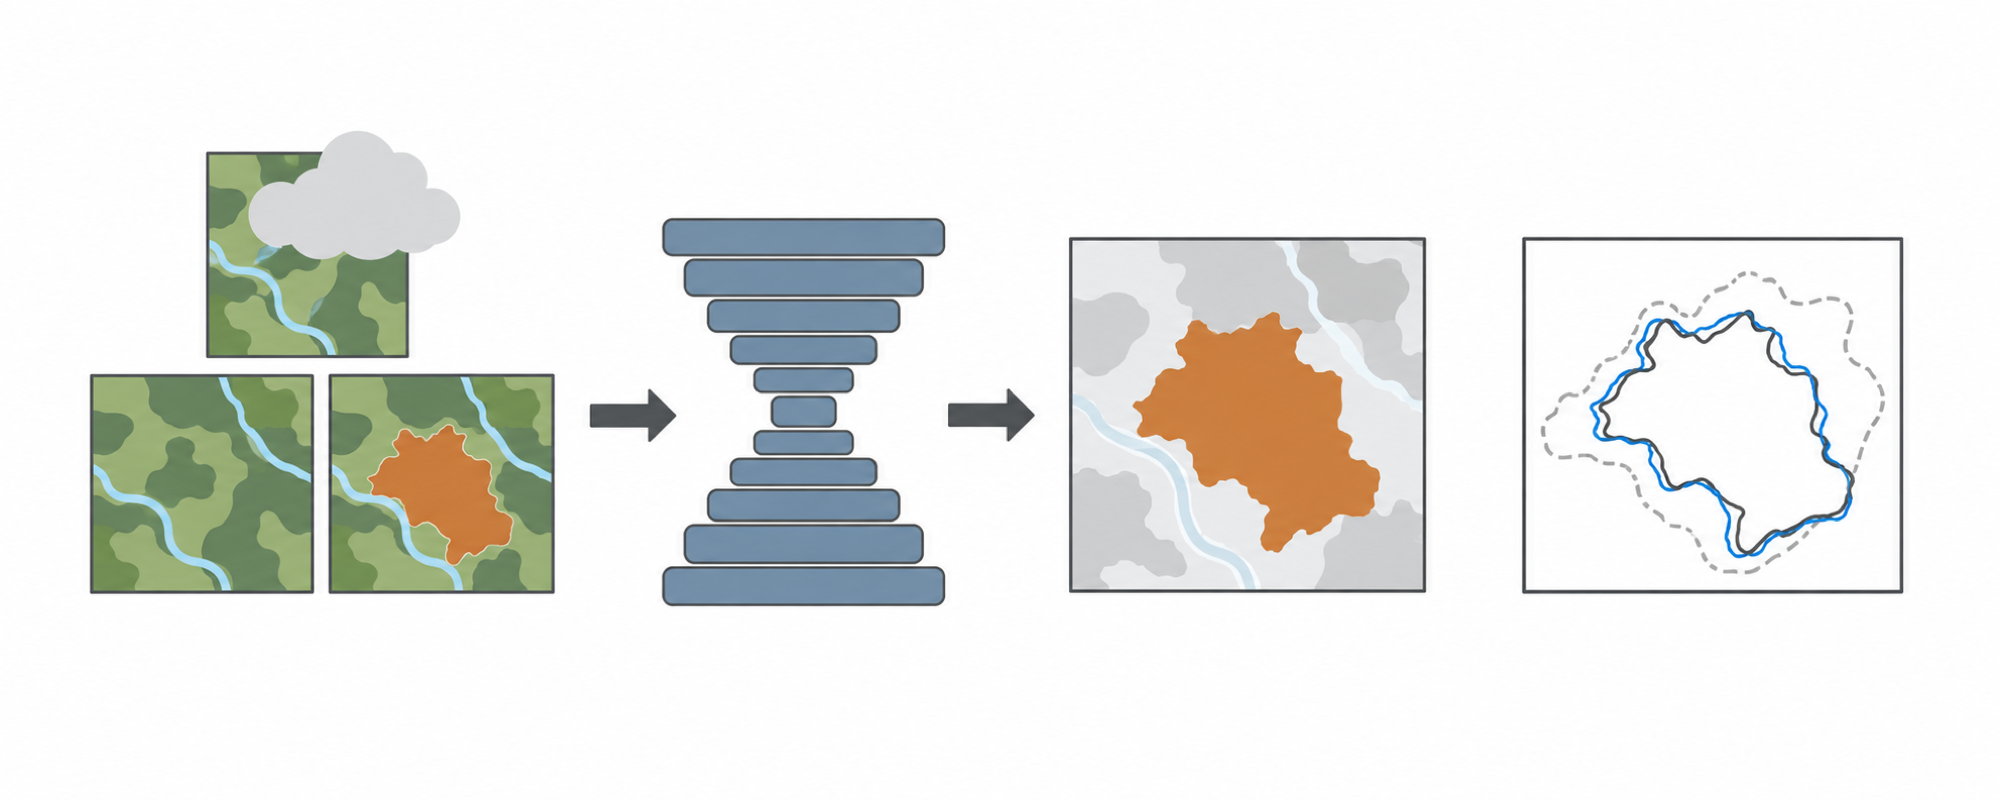
\includegraphics[width=\linewidth]{figures/ch10/ch10-03-composition-a-narrative.png}};
\begin{scope}[x={(img.south east)},y={(img.north west)}]
  \tikzset{stglbl/.style={font=\sffamily\footnotesize\bfseries,text=BookInk,fill=white,fill opacity=0.90,text opacity=1,inner sep=1.5pt,align=center}}
  \node[stglbl] at (0.165,0.16) {(1) 输入影像与云遮挡};
  \node[stglbl] at (0.40,0.16) {(2) 分割网络};
  \node[stglbl] at (0.62,0.16) {(3) 过火区图};
  \node[stglbl] at (0.855,0.16) {(4) 边界对比};
\end{scope}
\end{tikzpicture}
\caption{构图候选 A：左$\rightarrow$右叙事式。输入、模型、输出、发现四段从左到右展开，阅读起点唯一，终点落在边界比较示意；云图块把“需要无云观测”放在读者必经的输入端。底图由图像模型生成，所有影像均为示意图块。}\label{fig:ch10-03}
\end{figure}

核对图~\ref{fig:ch10-03} 的实际画面：四段齐全，左侧火前、火后图块的河流转折位置一致，上方叠放了云遮挡图块；中间为单列 10 层圆角矩形组成的蓝灰沙漏；(1)$\rightarrow$(2) 与 (2)$\rightarrow$(3) 之间为两支同型深灰实心箭头，(3) 与 (4) 之间无箭头；最右侧对比框内深灰实线、蓝实线与向外偏离的浅灰虚线关系清楚。细看也有几处轻微偏差：上方云朵本身画得偏大并略微探出图块顶框；四段并非严格等宽（并排输入图块右缘到约 $x=0.28$，而单个输出图块尺寸大于单块输入图块）；填色带有轻微明暗变化而非纯单色平涂。第二次生成虽把云朵改小，却丢掉了沙漏的深灰外框且各图块几何一致性变差，因此选定第一次生成结果。

再看\textbf{构图候选 B（中心图式）}：把阶段 (3) 的“过火区图”放大居中，把火前影像、火后影像（附云遮挡小图块）、分割网络与边界对比插图放在四角，用不带箭头头的细灰线连向中心图。英文提示词关键部分如下（完整版本见本书仓库 \texttt{cases/} 目录）：

\begin{Prompt}
Graphical abstract base art, wide banner, aspect ratio 5:2 (2000 x 800 px),
pure white background, flat 2D vector illustration, thin dark gray outlines.
ABSOLUTELY NO TEXT: no letters, words, numbers, symbols, labels or title.
Central composition. In the exact center, one large square top-down schematic
map tile (about 70% of image height) of a landscape patch in very pale gray with
a crisp warm brown-orange burned-area polygon and a thin pale-blue river line.
Around it, four small elements, each about one quarter the size of the center:
- upper left: small tile of the same patch in muted green vegetation (before);
- lower left: small tile of the same patch with a warm brown-orange area (after),
  and next to it an even smaller tile partly covered by a flat light gray cloud;
- upper right: small blue-gray hourglass shape of stacked rounded rectangles;
- lower right: small square inset with three boundary lines: dark gray solid,
  blue solid closely following it, light gray dashed clearly deviating.
Thin plain gray connector lines without arrowheads run from each small element
toward the central tile. Do not draw: flames, smoke, globes, satellites, clocks.
\end{Prompt}

中心图式生成了三次才合格，前两次落选恰好暴露了多元素环绕构图的常见失误：第 1 次生成时，中央大图保留了大片绿色植被而非浅灰底，且右上角网络被拆成了左右两列条块；第 2 次生成修好了浅灰中央图与单列沙漏，但左下角那根连接线竟直接连到了“云遮挡小图块”上，使真正的火后输入图块悬空游离；直到第 3 次在提示词中明确指定四根连线的接点位置并要求云图块独立脱开，才得到结构正确的候选 B（图~\ref{fig:ch10-04}）。

\begin{figure}[htbp]\centering
\begin{tikzpicture}
\node[anchor=south west,inner sep=0] (img) at (0,0) {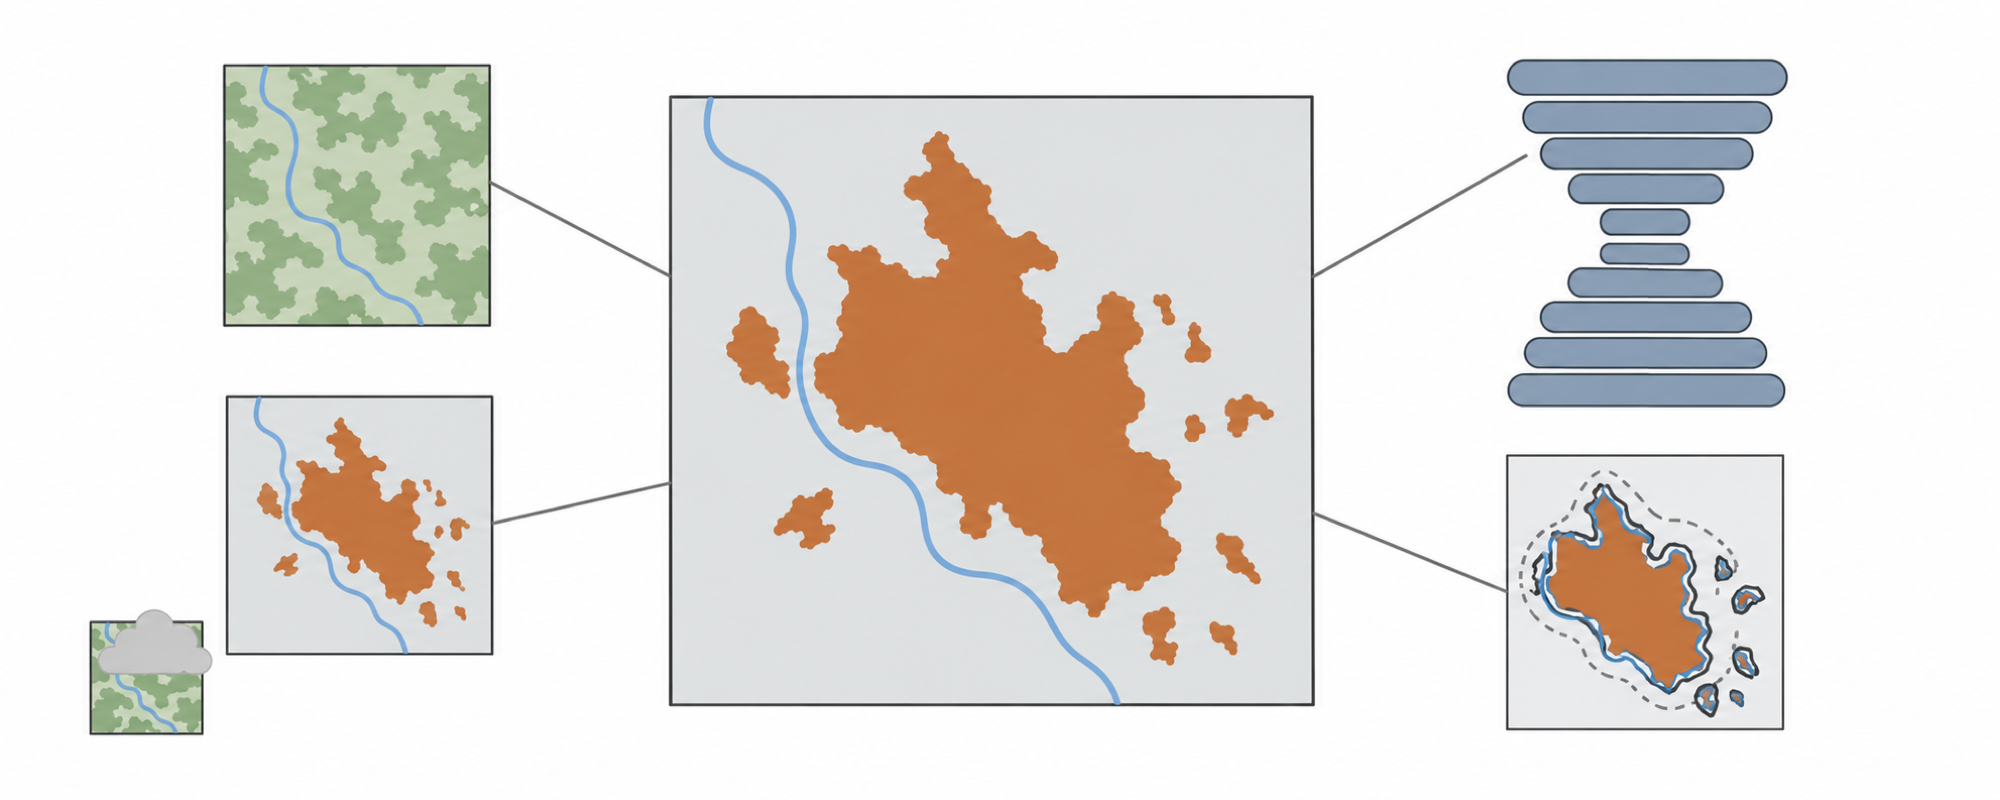
\includegraphics[width=\linewidth]{figures/ch10/ch10-04-composition-b-central.png}};
\begin{scope}[x={(img.south east)},y={(img.north west)}]
  \tikzset{stglbl/.style={font=\sffamily\scriptsize\bfseries,text=BookInk,fill=white,fill opacity=0.90,text opacity=1,inner sep=1.2pt,align=center}}
  \node[stglbl] at (0.175,0.54) {(1) 火前影像};
  \node[stglbl] at (0.175,0.11) {(1) 火后影像与云遮挡};
  \node[stglbl] at (0.82,0.45) {(2) 分割网络};
  \node[stglbl] at (0.49,0.05) {(3) 过火区图（中心）};
  \node[stglbl] at (0.82,0.04) {(4) 边界对比};
\end{scope}
\end{tikzpicture}
\caption{构图候选 B：中心图式。与图~\ref{fig:ch10-03} 内容相同。中心图吸引视线，但在 $5:2$ 横幅中，四周元素被压小，“比阈值法更贴近边界”的比较退到右下角落，在缩略图中最先看不清。\linebreak 若改投 $1200\ \text{px}$ 正方形格式，这种构图更容易适配。}\label{fig:ch10-04}
\end{figure}

观察图~\ref{fig:ch10-04} 也能看出中心图式在 $5:2$ 横幅中的局限：中央大图占了约 $77\%$ 的画布高度，四周元素被挤向左右两侧；右上角沙漏偏大，而右下角真正体现研究发现的边界对比插图被压得很小，内部细碎斑块与三条轮廓线在缩小时极易糊在一起；左下角的云遮挡小图块也退到了角落。表~\ref{tab:ch10-04-ab} 给出了两种构图的系统比较。

\begin{table}[htbp]\centering\footnotesize
\setlength{\tabcolsep}{3pt}
\renewcommand{\arraystretch}{1.15}
\caption{构图候选 A（左$\rightarrow$右叙事式）与候选 B（中心图式）的选型比较。}\label{tab:ch10-04-ab}
\begin{tabularx}{\linewidth}{@{}>{\raggedright\arraybackslash}p{24mm}YY@{}}
\toprule
\textbf{比较标准} & \textbf{候选 A：左$\rightarrow$右叙事式（图~\ref{fig:ch10-03}）} & \textbf{候选 B：中心图式（图~\ref{fig:ch10-04}）} \\
\midrule
阅读起点 & 唯一（最左侧火前/火后影像对） & 视线先落在中心大图，输入与对比分散在四周，起点不唯一 \\
终点是否为“发现” & 是（最右侧边界对比插图） & 中心图本身是“产出”，“优于阈值法”的对比被挤到右下角 \\
$5:2$ 横幅适配 & 好，四段横向展开，上下留出充足文字带 & 中心图高占约 $77\%$，上下难以排通栏文字，角落元素局促 \\
$200\ \text{px}$ 高缩略图 & 各阶段图标与主轮廓仍可辨 & 环绕的小元素与右下角细碎对比线在缩略图中最先消失 \\
限定条件位置 & 输入端上方云图标 + 底部通栏短句，读者顺路看到 & 云图标被挤到左下外角，易被忽略 \\
若改投 $1200\ \text{px}$ 正方形 & 需折成上下两行，阅读路径变 Z 字形 & 四角环绕中心大图的拓扑适配自然 \\
\midrule
\textbf{结论} & \textbf{选定 A}（本案例目标为 Elsevier 横幅） & {\raggedright 留作改投\newline 正方形格式时的备选} \\
\bottomrule
\end{tabularx}
\end{table}

两张候选图本身都干净整洁，最终选 A 而不是选 B，依据不是主观上的“哪张更好看”，而是画布长宽比、阅读起点与终点，以及限定条件在缩略图下的可见性。\linebreak
如果未来这篇论文改投要求提交 $1200 \times 1200\ \text{px}$ 正方形图形摘要的期刊，候选 B 的中心环绕布局反而更容易舒展。

\section{过度主张：当图像比论文说得更多}

假设合作者看了候选 A 后觉得“太素了，不够抢眼”，于是有人写了一句“让画面更震撼，突出 AI 的预警能力和全球意义”，提交了如下反例提示词：

\begin{Prompt}
Deliberately over-dramatic graphical abstract base art for a teaching
counter-example, wide banner, aspect ratio 5:2 (2000 x 800 px).
Dark blue gradient background with glowing accents.
Left: a photorealistic satellite-style top-down view of a forest with a bright
red-orange active fire front and thick gray smoke plumes.
Center: a glowing glossy 3D "AI brain" made of circuit lines, with light rays.
Right: a 3D Earth globe covered by a bright grid, with several red flame icons
on it, a red triangular alarm icon, and an alarm clock.
Glossy, cinematic, high contrast, lens flare.
NO TEXT: no letters, no words, no numbers, no symbols, no labels.
Leave a dark empty band across the top 18% for a headline.
\end{Prompt}

生成这张反例底图时有一个细节值得警惕：尽管提示词明确写了 \texttt{NO TEXT}，第 1 次生成仍在闹钟表盘上画出了 $1\text{--}12$ 数字并在红三角内画了感叹号，第 2 次生成在 12 点位置仍留下一条形似数字“1”的短刻线，直到第 3 次强制要求“空白表盘仅留两根指针、空心警报三角”才清掉所有内置字符。我们在第 3 次底图上用 TikZ 叠加上常见的夸大标题、百分比与预测口号（并附“虚构的夸大反例”水印防止截图误传），用红标 \textbf{O1—O7} 标出七处过度主张（图~\ref{fig:ch10-05}）。

\begin{figure}[htbp]\centering
\begin{tikzpicture}
\node[anchor=south west,inner sep=0] (img) at (0,0) {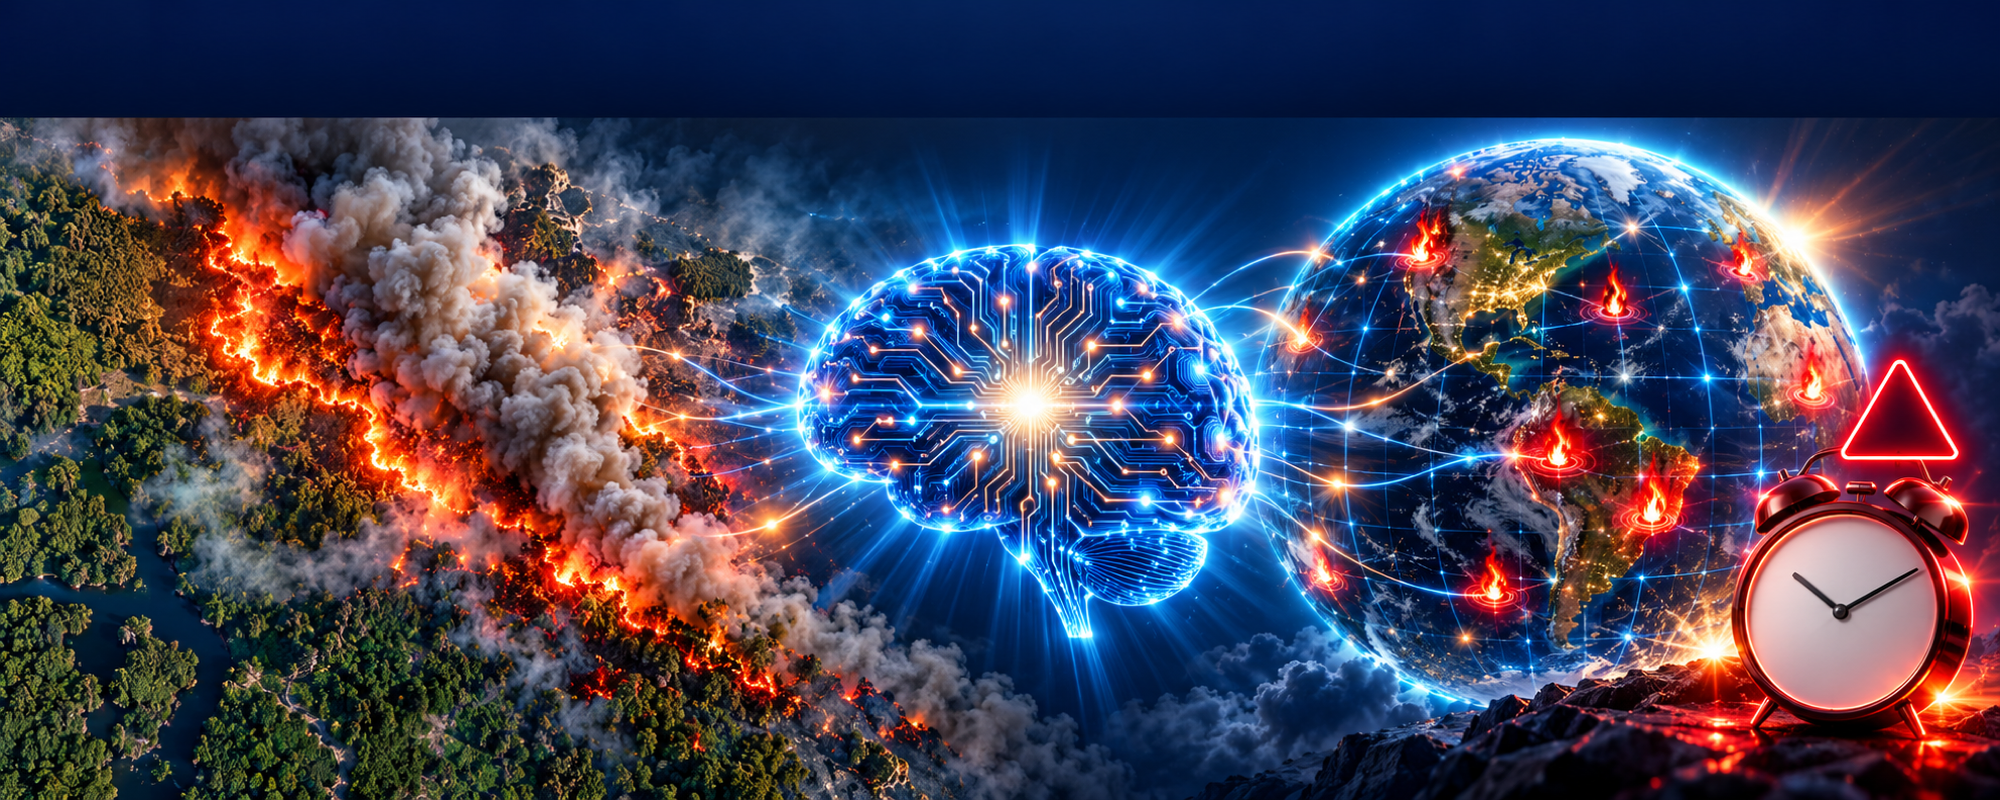
\includegraphics[width=\linewidth]{figures/ch10/ch10-05-overclaim.png}};
\begin{scope}[x={(img.south east)},y={(img.north west)}]
  \tikzset{
    overtxt/.style={font=\sffamily\bfseries,text=white,align=center},
    badmark/.style={draw=red!85!black,very thick,rounded corners=2pt,fill=white,fill opacity=0.92,text opacity=1,text=red!85!black,font=\sffamily\bfseries\scriptsize,inner sep=1.5pt}
  }
  \node[overtxt,font=\sffamily\normalsize\bfseries] at (0.52,0.92) {全球实时野火 AI（Real-time global wildfire AI）};
  \node[font=\sffamily\scriptsize\bfseries,text=yellow!90!white,fill=black!65,inner sep=1.5pt,rounded corners=1pt] at (0.50,0.81) {【虚构的夸大反例 · 非真实研究结果】};
  \node[overtxt,font=\sffamily\large\bfseries,text=yellow!95!white,fill=black!55,inner sep=2pt,rounded corners=2pt] at (0.50,0.45) {准确率 99\%};
  \node[overtxt,font=\sffamily\footnotesize\bfseries,fill=red!75!black,inner sep=2pt,rounded corners=2pt] at (0.72,0.12) {在起火前预测火灾};
  \node[badmark] at (0.09,0.34) {O1};
  \node[badmark] at (0.19,0.50) {O2};
  \node[badmark] at (0.77,0.56) {O3};
  \node[badmark] at (0.91,0.24) {O4};
  \node[badmark] at (0.37,0.45) {O5};
  \node[badmark] at (0.17,0.92) {O6};
  \node[badmark] at (0.27,0.70) {O7};
\end{scope}
\end{tikzpicture}
\caption{反例：过度主张的图形摘要（虚构示例）。照片质感的“卫星影像”、火线、地球、闹钟和无上下文的百分比，分别把“过火区制图”放大成观测证据、火点探测、全球覆盖、火灾预测和普适精度。图中的数字与标题均为故意夸大的虚构文字，不代表任何研究结果。底图由图像模型生成。}\label{fig:ch10-05}
\end{figure}

表~\ref{tab:ch10-05-overclaim} 逐项拆解了图~\ref{fig:ch10-05} 中 O1 至 O7 暗示的越界主张及保守修正方案。

\begin{table}[htbp]\centering\footnotesize
\setlength{\tabcolsep}{3pt}
\renewcommand{\arraystretch}{1.12}
\caption{图~\ref{fig:ch10-05} 中七处过度主张（O1--O7）的拆解与修正对照。}\label{tab:ch10-05-overclaim}
\begin{tabularx}{\linewidth}{@{}c>{\raggedright\arraybackslash}p{25mm}>{\raggedright\arraybackslash}p{25mm}>{\raggedright\arraybackslash}p{26mm}Y@{}}
\toprule
\textbf{\#} & \textbf{过度主张元素} & \textbf{它暗示了什么} & \textbf{论文实际支持什么} & \textbf{保守修正做法} \\
\midrule
O1 & 照片质感的森林俯视“影像” & 这是真实卫星观测照片 & 示意的火前/火后影像对；对象是已过火地表 & 改回扁平示意图块；图注说明“示意，非真实卫星影像” \\
O2 & 明亮火线、火焰图标与红色警报三角 & 活跃火点探测与应急报警 & 灾后已过火区域制图 & 删除火线、火焰与警报；过火区用暖棕橙色静态多边形 \\
O3 & 地球与覆盖全球的发光网格 & 全球各生态区通用 & 若干留出测试火场；跨生态区迁移未验证 & 删除地球与网格；只画单个示意地块并写明测试范围 \\
O4 & 闹钟与“在起火前预测火灾” & 能在起火前预测火灾发生 & 火后第一景无云影像到达后制图 & 删除闹钟与“预测”；改为“火后第一景无云影像即可绘制过火区” \\
O5 & 大号“准确率 99\%” & 有一个普适的高精度数字 & 仅报告比固定阈值基线更接近参考边界；数字需指标与对照 & 删除数字；用右侧三条边界线的贴合对比表达比较结论 \\
O6 & “全球实时野火 AI”标题 & 全球覆盖、实时响应 & 受重访周期与云烟限制 & 标题改为“火后第一景无云影像即可绘制过火区” \\
O7 & 浓烟滚滚却被 AI 光束直接穿透，且隐去无云限制 & 不受云烟遮挡、可全天候穿透观测 & 光学波段受云烟遮挡时一致性下降，依赖无云观测 & 删除穿透浓烟的光束；在输入端加回灰云遮挡图块与底部限定句 \\
\bottomrule
\end{tabularx}
\end{table}

特别注意 \textbf{O7}：画面左侧画了立体浓烟遮蔽森林，中央发光大脑的光束却直接穿透浓烟连向全球网格，同时把“需无云观测”的云朵图块删得一干二净，让人误以为光学波段能穿透浓烟作业。

\begin{BookNote}
\textbf{原则：图形摘要中的每一个图标都是一句陈述。}审稿人和读者会把“火焰”读作“探测火点”，把“地球”读作“全球通用”，把“闹钟”读作“事前预警”，把“穿透浓烟的光束”读作“不受云烟限制”。检查时把每个视觉元素翻译成一句陈述，再到论文里找它的依据，找不到就删。
\end{BookNote}

遇到图~\ref{fig:ch10-05} 这种整体跑偏的夸大稿，不要拿它当参考图局部修补，而应\textbf{直接退回候选 A 底图（图~\ref{fig:ch10-03}）}，下达如下精确微调指令：

\begin{Prompt}
以 A 稿为基础，不使用刚才的“震撼版”。保持 A 稿四段布局与所有对象不变。
不要火焰、烟柱、红色警报、地球、闹钟、照片质感影像，不要任何数字或文字。
只做两处修改：(1) 输出过火区图略放大约 1.2 倍；(2) 对比插图中三条边界线加粗，
使浅灰虚线与蓝色实线的偏离在缩小后仍可见。
\end{Prompt}

\section{定稿、缩略图测试与终稿核验}

我们按上述修改要求编写终稿英文提示词（完整版本见本书仓库 \texttt{cases/} 目录）：

\begin{Prompt}
Final graphical abstract base art, wide banner, aspect ratio 5:2,
2000 x 800 px, pure white background, flat 2D vector illustration, flat fills,
uniform thin dark gray (#3A3A3A) outlines, no gradients, no shadows, no 3D.
THIS IMAGE MUST CONTAIN NO TEXT AT ALL: no letters, words, numbers, symbols.
EMPTY BANDS: keep y 0.00-0.15 (top), y 0.76-0.84 (caption strip under the four
stages) and y 0.88-1.00 (bottom) completely white.
Four stages, all objects vertically within y 0.18-0.72:
1. x 0.04-0.25: two square schematic map tiles side by side (left: muted green
   #A8C3A0 vegetation; right: same patch with #C8743C burned area), same river.
   Smaller tile partly covered by a flat light gray (#D5D5D5) cloud at upper left.
2. x 0.30-0.45: one blue-gray (#8FA3B8) hourglass of stacked rounded rectangles.
3. x 0.50-0.73: one larger square map tile in very pale gray with a crisp
   #C8743C burned-area polygon (about 1.2 times the input tiles).
4. x 0.77-0.96: a square inset with three thick boundary lines: #3A3A3A solid
   (reference), #2F6DB5 solid closely following it, #A0A0A0 dashed deviating.
Two identical #3A3A3A arrows: stage 1 -> 2, stage 2 -> 3; no arrow between 3 and 4.
\end{Prompt}

终稿底图同样生成了三次：前两次未挂参考图独立生成时，第 1 次把沙漏网络画成了左右分开的 X 形双列且虚线偏离不够明显，第 2 次虽修好网络并加粗了边界线，但随机生成的河流与过火区形状与候选 A 不同；第 3 次\textbf{以候选 A（图~\ref{fig:ch10-03}）作为视觉参考图}生成，完整保留了候选 A 的河流走向、过火区轮廓、单列沙漏和两支流程箭头，同时将阶段 (4) 的三条对比边界线显著加粗。实测检查也记录下三处细微残余偏差：输出图块边长约为单块输入图块的 $1.6$ 倍（与左侧上下两层图块总高视觉齐平，而非严格 $1.2$ 倍）、部分图框下缘到约 $y=0.75$、留白带像素 RGB 在 $249\text{--}255$ 之间轻微浮动。这些几何与底色细节不影响科学表达，且三条文字空白带干净可用。

接着在无文字底图上用 TikZ 叠加七处矢量文字（表~\ref{tab:ch10-06-text}），得到图形摘要终稿（图~\ref{fig:ch10-06}）。

\begin{table}[htbp]\centering\footnotesize
\setlength{\tabcolsep}{3pt}
\renewcommand{\arraystretch}{1.15}
\caption{图形摘要终稿（图~\ref{fig:ch10-06}）叠加的矢量文字层（T1--T7）中英对照。}\label{tab:ch10-06-text}
\begin{tabularx}{\linewidth}{@{}cYY>{\raggedright\arraybackslash}p{28mm}@{}}
\toprule
\textbf{\#} & \textbf{中文文字层} & \textbf{英文文字层} & \textbf{位置与字号层级} \\
\midrule
T1 & 火后第一景无云影像即可绘制过火区 & Burned-area maps from the first clear post-fire image & $(0.50,0.07)$ 顶部居中；最大字号 \\
T2 & 火前 / 火后 Sentinel-2 影像对 & Pre-/post-fire Sentinel-2 pair & 阶段 (1) 下方；中号（缩略图可读） \\
T3 & 分割网络 & Segmentation network & 阶段 (2) 下方；中号（缩略图可读） \\
T4 & 过火区图 & Burned-area map & 阶段 (3) 下方；中号（缩略图可读） \\
T5 & 比 dNBR 阈值法更贴近参考边界 & Closer to reference edges than dNBR threshold & 阶段 (4) 下方；中号（缩略图可读） \\
T6 & 绘制已过火区域 · 非火点探测或预测 · 需无云观测 & Maps areas already burned $\cdot$ not fire detection or forecasting $\cdot$ needs cloud-free views & $(0.50,0.94)$ 底部居中；小号（文章页可读） \\
T7 & 参考 / 模型 / 阈值法 & reference / model / threshold & 对比插图下方小图例；最小字号 \\
\bottomrule
\end{tabularx}
\end{table}

\begin{figure}[htbp]\centering
\begin{tikzpicture}
\node[anchor=south west,inner sep=0] (img) at (0,0) {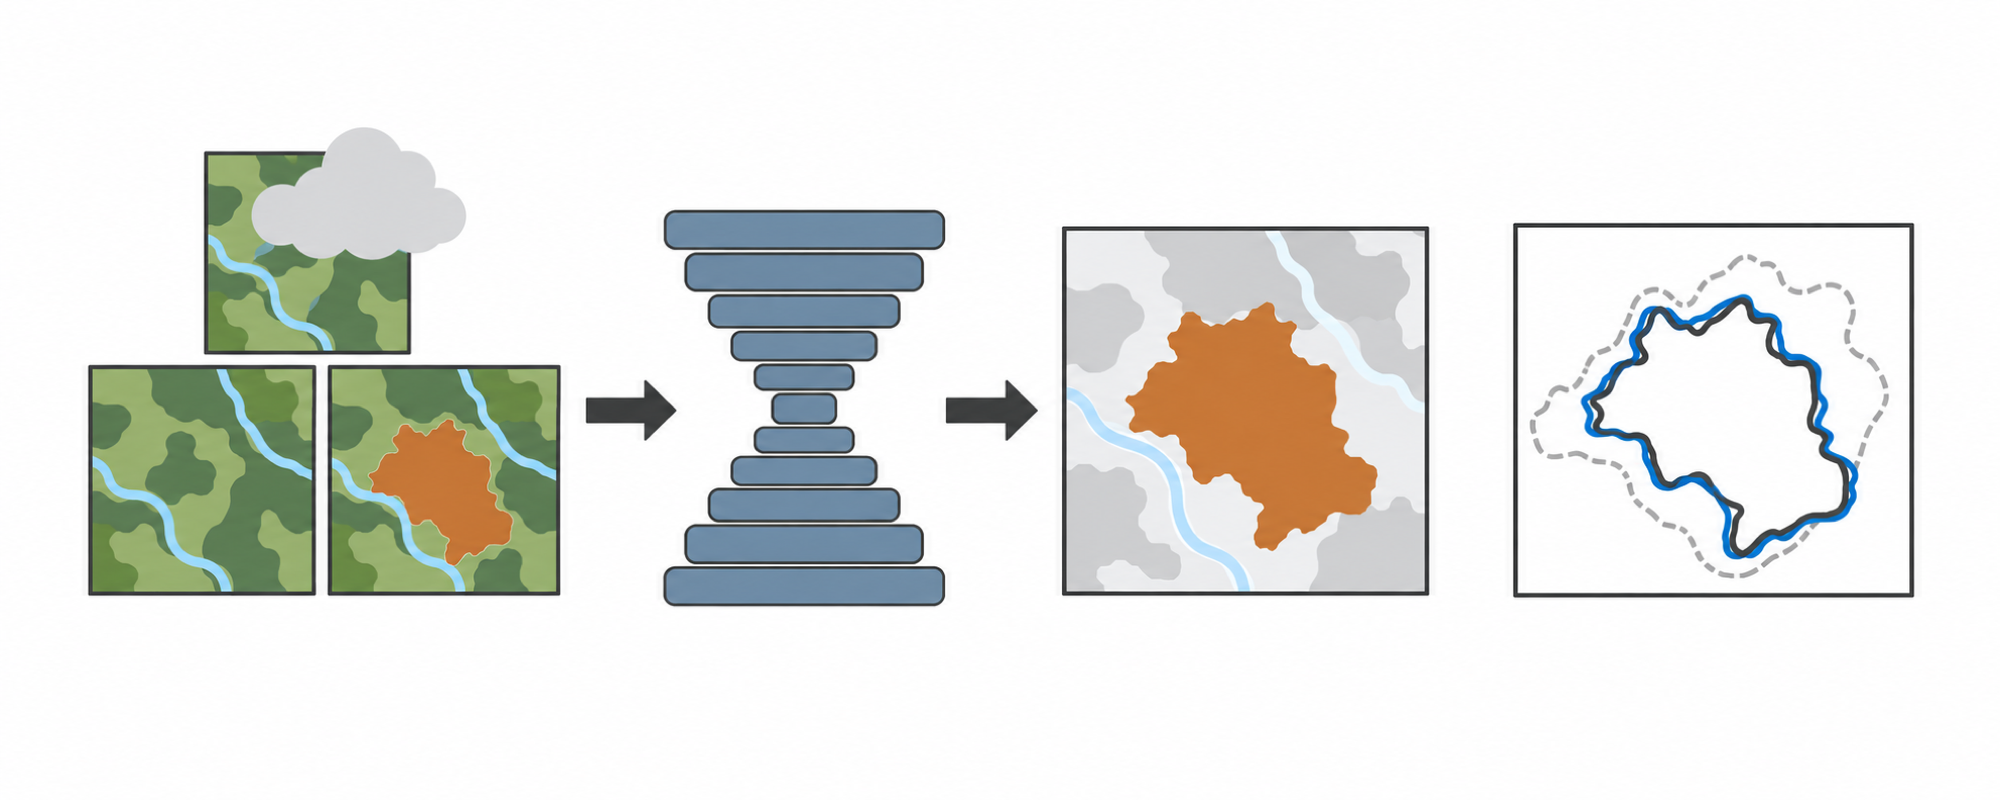
\includegraphics[width=\linewidth]{figures/ch10/ch10-06-final-base.png}};
\begin{scope}[x={(img.south east)},y={(img.north west)}]
  \tikzset{
    t1style/.style={font=\sffamily\small\bfseries,text=BookInk,align=center},
    tstg/.style={font=\sffamily\scriptsize\bfseries,text=BookInk,fill=white,fill opacity=0.90,text opacity=1,inner sep=1pt,align=center},
    t6style/.style={font=\sffamily\scriptsize,text=BookInk!90,align=center},
    t7style/.style={font=\sffamily\tiny,text=BookInk!85,align=center}
  }
  \node[t1style] at (0.50,0.92) {火后第一景无云影像即可绘制过火区};
  \node[tstg] at (0.165,0.18) {火前 / 火后 Sentinel-2 影像对};
  \node[tstg] at (0.40,0.18) {分割网络};
  \node[tstg] at (0.62,0.18) {过火区图};
  \node[tstg] at (0.855,0.18) {比 dNBR 阈值法更贴近参考边界};
  \node[t7style] at (0.855,0.11) {参考 / 模型 / 阈值法};
  \node[t6style] at (0.50,0.04) {绘制已过火区域 · 非火点探测或预测 · 需无云观测};
\end{scope}
\end{tikzpicture}
\caption{教学案例的图形摘要终稿。左$\rightarrow$右依次为火前/火后影像对、分割网络、过火区图，以及与参考边界的比较示意。底部一句写明限定条件。全部影像均为扁平示意图块，\textbf{非真实卫星影像}；研究情境为本章虚构的教学案例，不对应已发表结果。底图由图像模型生成，文字以 TikZ 叠加。}\label{fig:ch10-06}
\end{figure}

最后一步是把“缩到目录尺寸还看得清吗”变成可重复的\textbf{缩略图测试（thumbnail test）}。当 $2000 \times 800\ \text{px}$ 的原图被缩放到 Elsevier 指南所述的 $200\ \text{px}$ 高目录窗口（即 $500 \times 200\ \text{px}$）时，线性尺寸缩小为原来的四分之一。若原图阶段名采用约 $36\ \text{px}$ 字高，缩后约为 $9.0\ \text{px}$ 高，仍可辨认；若原图只用 $14\ \text{px}$ 字高，缩后仅剩约 $3.5\ \text{px}$ 高，笔画彻底糊成一团（图~\ref{fig:ch10-07}）。同时注意，关键限定条件必须像 T6 这样写在图内（配合左上角云图标），不能只写在图外图注里。

\begin{figure}[htbp]\centering
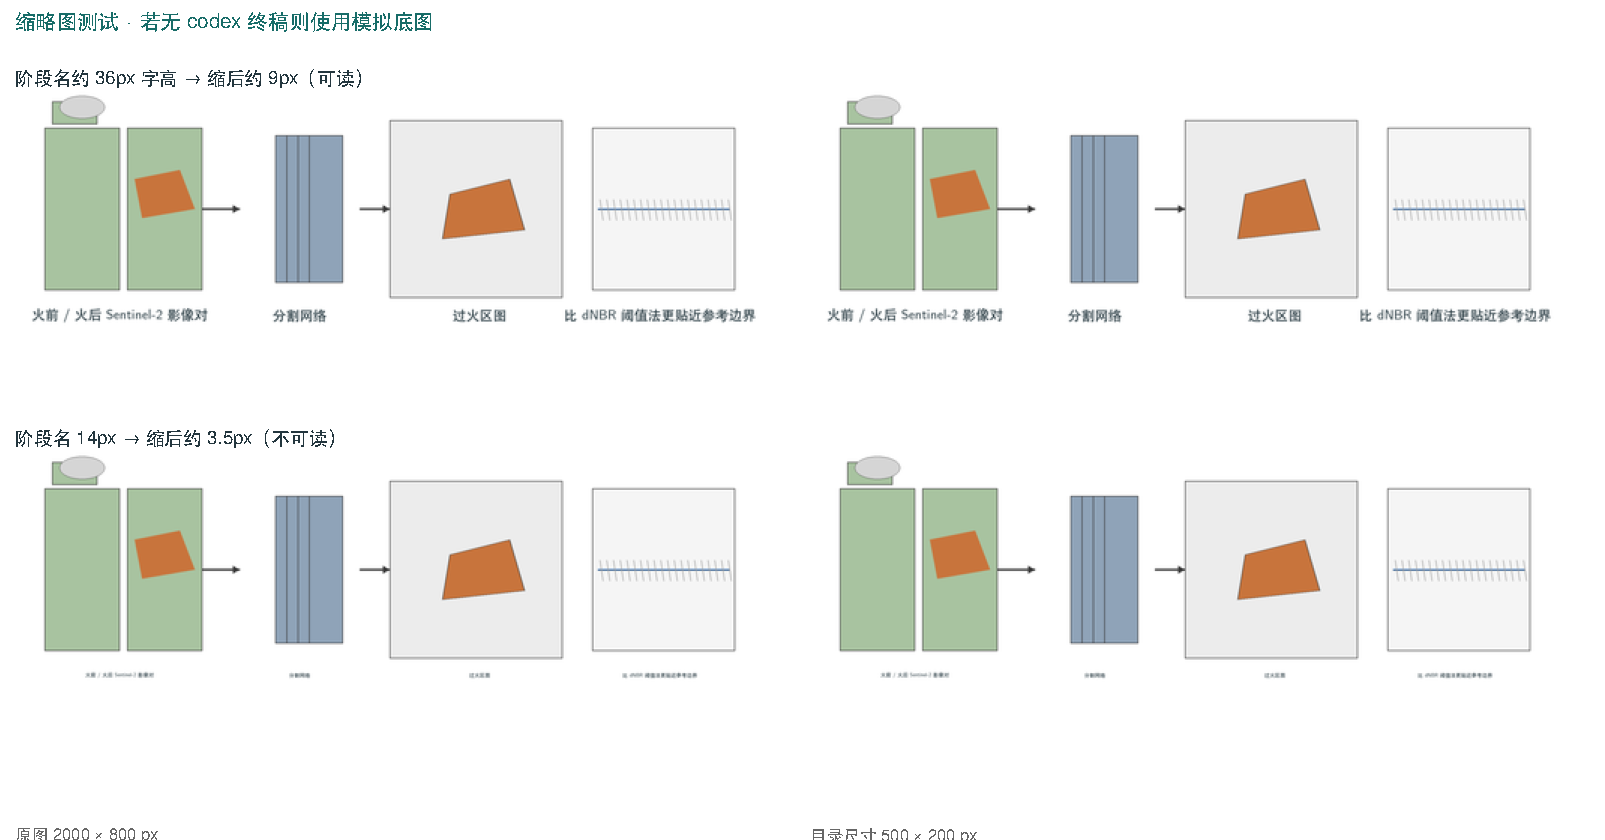
\includegraphics[width=\linewidth]{figures/ch10/ch10-07-thumbnail-test-zh.pdf}
\caption{缩略图测试。把图形摘要缩到约 $200\ \text{px}$ 高（Elsevier 指南所述的目录显示高度）后，以实际像素显示（本图在相同 $2000 \times 800\ \text{px}$ 模拟布局底图上仅改变阶段名字高进行对照）。上：阶段名约 $36\ \text{px}$ 字高，缩后约 $9\ \text{px}$ 高，仍可辨认；下：同一张图只把阶段名改小为 $14\ \text{px}$，缩小后约 $3.5\ \text{px}$ 高，已无法阅读。底部限定句在缩略图中较小，但在文章页中可读。}\label{fig:ch10-07}
\end{figure}

\section{本章完整案例回顾与核验表}

回顾本案例，我们从一篇虚构教学摘要出发，依次完成了期刊规格核查（图~\ref{fig:ch10-01}）、四行贡献卡提炼（表~\ref{tab:ch10-02-card}）、PDF 转提示词边界比对（图~\ref{fig:ch10-02}、表~\ref{tab:ch10-03-compare}）、A/B 两种构图比选（图~\ref{fig:ch10-03}、图~\ref{fig:ch10-04}、表~\ref{tab:ch10-04-ab}）、过度主张反例拆解（图~\ref{fig:ch10-05}、表~\ref{tab:ch10-05-overclaim}）、终稿底图修改与矢量叠字（图~\ref{fig:ch10-06}），以及 $200\ \text{px}$ 高缩略图实测（图~\ref{fig:ch10-07}）。终稿交付前的九项核验记录汇总于表~\ref{tab:ch10-07-verify}。

\begin{table}[htbp]\centering\footnotesize
\setlength{\tabcolsep}{3pt}
\renewcommand{\arraystretch}{1.15}
\caption{教学案例图形摘要终稿（图~\ref{fig:ch10-06}）的九项核验表（C1--C9）。}\label{tab:ch10-07-verify}
\begin{tabularx}{\linewidth}{@{}c>{\raggedright\arraybackslash}p{26mm}>{\raggedright\arraybackslash}p{32mm}Y@{}}
\toprule
\textbf{\#} & \textbf{检查项} & \textbf{核验方法} & \textbf{结果记录} \\
\midrule
C1 & 贡献卡四行都在图中 & 逐行指出对应元素 & 问题与方法对应阶段 (1)--(3) 及 T1--T4；发现对应阶段 (4) 与 T5；限定对应左上灰云图块与底部 T6 短句 \\
C2 & 无超出论文的元素 & 把每个图标翻译成一句话并在摘要中找依据 & 全部对象均为任务书规定的示意元素，无火焰、地球、闹钟或百分比数字 \\
C3 & 无数字、无数据图、无照片质感影像 & 放大检查纹理与图形类别 & 无数字与数据图；影像为扁平示意图块（填色带轻微明暗变化，图注已标明非真实卫星影像） \\
C4 & 比例与像素 & 检查文件属性：$5:2$，$\ge 1328 \times 531\ \text{px}$ & 交付底图为 $2000 \times 800\ \text{px}$，满足 $5:2$ 比例与像素要求 \\
C5 & 缩略图可读 & 图~\ref{fig:ch10-07} 测试：$200\ \text{px}$ 高下阶段名可读 & 阶段名按约 $36\ \text{px}$ 字高设置，缩至 $200\ \text{px}$ 高后约 $9\ \text{px}$ 高，可辨认 \\
C6 & 底图无伪文字 & 原尺寸放大检查 & 选定底图未见字母、数字或伪文字（反例图前两次出现的表盘数字与刻线已淘汰重出） \\
C7 & 中英两版只有文字层不同 & 比对底图文件哈希值 & 中英两版共用同一无字底图文件，仅 TikZ 叠加文字层按表~\ref{tab:ch10-06-text} 切换 \\
C8 & 期刊要求已在提交前复核 & 记录目标期刊页面 URL 与访问日期 & 已记录 Elsevier 通用指南 URL 与 2026 年 10 月访问日期；投具体子刊前须再次复核 \\
C9 & PDF 转提示词的读取范围与原文已存档 & 检查本地图片档案记录 & 使用 \sdtool{graphical-abstract-maker} 时，将前 5 页读取范围、返回提示词原文与比对表一并存档 \\
\bottomrule
\end{tabularx}
\end{table}

\section{AI 在这一步能做什么与不能做什么}

图形摘要制作各环节中 AI 与作者的职责边界汇总于表~\ref{tab:ch10-08-ai}。

\begin{table}[htbp]\centering\footnotesize
\setlength{\tabcolsep}{3pt}
\renewcommand{\arraystretch}{1.15}
\caption{图形摘要制作环节中 AI 能做什么、不能做什么与作者要核对的内容。}\label{tab:ch10-08-ai}
\begin{tabularx}{\linewidth}{@{}>{\raggedright\arraybackslash}p{16mm}YYY@{}}
\toprule
\textbf{环节} & \textbf{AI（\scidraw{} 等）能做} & \textbf{AI 不能做} & \textbf{作者要核对} \\
\midrule
读论文 & 图形摘要入口读取 PDF 前 5 页（约 $6{,}000$ 字符以内），生成 $60\text{--}110$ 词视觉提示词 & 理解全文；判断哪个发现最重要；保证保留限定条件 & 记录读取范围与输出原文；与贡献卡逐行比对，补回限定条件 \\
提炼贡献 & 帮你把摘要改写成更短的句子；列出可能的视觉对象 & 决定论文的核心贡献；判断措辞强度是否与证据相符 & 每一行能否在论文中找到原句；“优于”“解决”“预测”等词是否越界 \\
构图 & 按提示词生成同一构图的多个候选；按要求生成第二种构图 & 自动提出“有理由的”不同构图并解释取舍（批量候选只是随机变体） & 两种构图分别写明；用比例、阅读路径、缩略图、限定条件可见性比较 \\
生成底图 & 扁平示意风格、无字底图、留白区域（结果有随机性） & 保证无伪文字；精确位置；保证示意影像不被读成真实观测 & 放大查伪文字；影像必须是示意风格并在说明中注明 \\
修改 & 以历史图为参考图按指令修改 & 对象锁定；保证只改指定处 & 每次修改后重做整张核验（见第 11 章） \\
文字 & （不建议）在图中生成文字 & 可靠拼写与对位 & 文字用 TikZ 或排版软件叠加；逐字比对 \\
交付 & 导出图片 & 判断目标期刊当前要求 & 打开目标期刊页面核对比例、像素、字体、格式并记录日期；缩略图测试 \\
诚信 & — & 判断某个图标是否构成过度主张 & 把每个元素翻译成一句陈述，在论文中找依据 \\
\bottomrule
\end{tabularx}
\end{table}

\section{本章检查清单}

\begin{itemize}
\item 已打开目标期刊\textbf{当前}的图形摘要要求页面，记录了 URL、访问日期、比例、像素、字体与格式。
\item 贡献卡四行（问题 / 方法 / 发现 / 限定）都能在论文中找到原句，措辞强度没有升级。
\item 若使用了 PDF 转提示词：已存档读取范围（前 5 页）与输出原文，并逐行比对、补回限定条件。
\item 至少有两种\textbf{写明理由}的构图候选，并按比例、阅读起点与终点、缩略图可读性、限定条件位置选定。
\item 图中每个图标都能翻译成论文支持的一句话；没有火焰、地球、闹钟、数字一类“替你多说话”的元素，除非论文确实支持。
\item 示意影像不是照片质感；如使用真实影像，来源、许可与处理已写明。
\item 底图无伪文字；文字全部叠加并逐字核对；总字数克制。
\item 缩到目录尺寸（如 $200\ \text{px}$ 高）后阶段名仍可读，阅读路径清楚。
\item 中英两版只在文字层不同。
\item 档案中记录了工具、提示词、生成次数和人工修改。
\end{itemize}

\section{练习}

\begin{enumerate}
\item \textbf{（贡献卡：纸笔练习）}选一篇你所在领域近期的论文，只读摘要和结论，写出四行贡献卡；再通读结果部分，修改“发现”与“限定”两行。比较两次的差别，并说明哪一处措辞如果写进图形摘要会构成过度主张。
\item \textbf{（\scidraw{} 实操：PDF 转提示词的比对）}打开 \scidraw{} 的图形摘要工具 \sdtool{graphical-abstract-maker}，上传你自己（或练习 1）的论文 PDF，保存返回的视觉提示词。做一张比对表：贡献卡每一行在提示词中是“保留”“丢失”还是“被加强”。据此写出修改后的生成提示词，生成一版候选，并完成本章检查清单。
\item \textbf{（改格式）}把本章终稿（$5:2$）改成 $1200 \times 1200\ \text{px}$ 正方形的方案：画出草图，说明你会改用候选 A 的两行折叠还是候选 B 的中心图式、限定条件放在哪里，以及缩略图测试应怎样调整。
\end{enumerate}

\section*{参考文献}

\begin{itemize}
\item American Chemical Society. \textit{The Journal of Organic Chemistry} Author Guidelines. \url{https://researcher-resources.acs.org/publish/author_guidelines?coden=joceah} (accessed 2026-10-29).
\item American Chemical Society. \textit{Langmuir} Author Checklist. \url{https://pubs.acs.org/page/langd5/submission/author-checklist} (accessed 2026-10-29).
\item Cell Press. Attract readers at a glance with your Graphical Abstract. \url{https://crosstalk.cell.com/blog/attract-readers-at-a-glance-with-your-graphical-abstract} (accessed 2026-10-29).
\item Cell Press. \textit{Cell Reports} Final File Requirements. \url{https://www.cell.com/pb-assets/journals/EM/MasterFFCs/CELREPFFC-1750868285900.pdf} (accessed 2026-10-29).
\item Chuvieco E, Mouillot F, van der Werf GR, et al. Historical background and current developments for mapping burned area from satellite Earth observation. \textit{Remote Sensing of Environment}. 2019;225:45--64. \url{https://doi.org/10.1016/j.rse.2019.02.013}
\item Elsevier. Graphical abstracts — Author tools and resources. \url{https://www.elsevier.com/researcher/author/tools-and-resources/graphical-abstract} (accessed 2026-10-29).
\item Giglio L, Boschetti L, Roy DP, Humber ML, Justice CO. The Collection 6 MODIS burned area mapping algorithm and product. \textit{Remote Sensing of Environment}. 2018;217:72--85. \url{https://doi.org/10.1016/j.rse.2018.08.005}
\item Ibrahim AM, Lillemoe KD, Klingensmith ME, Dimick JB. Visual abstracts to disseminate research on social media: a prospective, case-control crossover study. \textit{Annals of Surgery}. 2017;266(6):e46--e48. \url{https://doi.org/10.1097/SLA.0000000000002277}
\item Knopp L, Wieland M, Rättich M, Martinis S. A deep learning approach for burned area segmentation with Sentinel-2 data. \textit{Remote Sensing}. 2020;12(15):2422. \url{https://doi.org/10.3390/rs12152422}
\item Pferschy-Wenzig E-M, Pferschy U, Wang D, Mocan A, Atanasov AG. Does a graphical abstract bring more visibility to your paper? \textit{Molecules}. 2016;21(9):1247. \url{https://doi.org/10.3390/molecules21091247}
\item Roy DP, Huang H, Boschetti L, et al. Landsat-8 and Sentinel-2 burned area mapping — a combined sensor multi-temporal change detection approach. \textit{Remote Sensing of Environment}. 2019;231:111254. \url{https://doi.org/10.1016/j.rse.2019.111254}
\end{itemize}

% TODO: 1) SciDraw AI `/zh/graphical-abstract-maker` 上传 `teaching-paper.pdf` 的在线实测返回提示词（`provenance/ch10/pdf-prompt.txt`）待补测归档；
% TODO: 2) `figures/ch10/ch10-07-thumbnail-test-zh.pdf` 当前使用脚本内置的模拟底图（`simulated_base: true`），待接入 `ch10-06-final-base.png` 合成终稿后重新生成；
% TODO: 3) Cell Press 总指南页（`https://www.cell.com/figureguidelines`）此前被访问验证拦截，以及 ACS 通用图形指南“字号不小于 8 pt”条款，待人工打开原始页面复核。

\chapter{把“再好看一点”变成可执行的修改}
\usetikzlibrary{decorations.pathmorphing}

土木工程专业的硕士生小陈正在写学位论文第 2 章（方法部分），需要一张斜拉桥结构健康监测传感网络的系统架构示意图，用来交代传感器布设位置、无线汇聚网关、云端分析流程与管理终端预警路径。他把第一版示意图发给导师，半小时后收到回复：“再好看一点，现在看着有点乱，不够专业。”

小陈立刻回到图像生成工具，换了一套深蓝色调的科技风背景，给桥塔加上立体阴影和发光无线波纹，导出第二版发过去，导师看后还是摇头；到了第三版，为了“让画面清爽一点”，他让工具“把杂乱的无线信号线改清楚”，结果生成模型在重绘整张图时悄悄抹掉了一根斜拉索和右塔顶的卫星定位天线。小陈自己只盯着改过的无线虚线看，直到周末组会放映幻灯片时才被同门师兄当场指出。

收到笼统的审阅意见就盲目重画，每次局部修改后又只看改过的那一处，是科研配图反复返工甚至把对的地方改错的两个主要根源。本章围绕这一痛点，说明如何把模糊的审阅直觉拆解为分级、可定位的修改单，如何在生成式修改与排版层修改之间分工，以及如何用整图复核与版本树拦截“改一处、动全图”的连带变化。

\section{三层问题：先对，再清楚，最后统一}

拿到导师、合作者或审稿人退回的配图初稿时，最忌讳按对方说话的先后顺序想到哪儿改到哪儿。有人先花两小时调整字体和配色，回头才发现箭头方向画反了；有人为了让画面“更有视觉冲击力”，在重生成时把原本画对的构件数量改错了。

要让修改过程收敛，第一步是把图中所有潜在问题划分为三个层级，并严格按照**先科学错误、再阅读障碍、最后视觉一致性**的顺序处理（图~\ref{fig:ch11-01}）。

\begin{figure}[htbp]\centering
\resizebox{\linewidth}{!}{% FIG ch11-01 three levels (Chinese)
\usetikzlibrary{arrows.meta,positioning,calc}
\begin{tikzpicture}[x=\linewidth/100,y=\linewidth/100]
\begin{scope}[
  font=\sffamily\small,
  level/.style={
    draw=BookRule, line width=0.5pt, rounded corners=2pt,
    minimum width=52mm, minimum height=11mm, align=left, inner sep=4pt,
    text width=50mm, anchor=west,
  },
  qbox/.style={
    draw=BookRule, fill=BookPale!40, rounded corners=2pt,
    align=center, inner sep=3pt, text width=22mm, font=\scriptsize,
  },
]
  \node[
    draw=BookTeal, line width=0.7pt, fill=white, rounded corners=3pt,
    align=center, inner sep=5pt, text width=24mm, font=\small,
  ] (bubble) at (8,42) {再好看一点};
  \draw[BookInk!55, dashed, -{Stealth[length=2mm]}] (bubble.east) -- (22,42);

  \node[qbox] (q1) at (32,58) {视线\\停在哪？};
  \node[qbox, below=3mm of q1] (q2) {读者会\\误解哪里？};
  \node[qbox, below=3mm of q2] (q3) {哪些本应\\一样却不一样？};

  \foreach \q in {q1,q2,q3} {
    \draw[BookInk!45, -{Stealth[length=1.6mm]}] (\q.east) -- ++(6,0);
  }

  \node[level, fill=BookInk, text=white] (L1) at (54,66) {%
    \textbf{第 1 层　科学错误}\\[-1pt]
    {\scriptsize 例：画成了悬索桥；数据箭头方向反了}\\
    {\scriptsize\textcolor{BookPale!90}{处理：回到任务书，必要时重新生成}}};
  \node[level, fill=BookInk!60, text=BookInk, below=2.5mm of L1] (L2) {%
    \textbf{第 2 层　阅读障碍}\\[-1pt]
    {\scriptsize 例：无线链路像拉索；160\,mm 下图标太小}\\
    {\scriptsize 处理：一次只改一类问题}};
  \node[level, fill=BookInk!30, text=BookInk, below=2.5mm of L2] (L3) {%
    \textbf{第 3 层　视觉一致性}\\[-1pt]
    {\scriptsize 例：同类传感器颜色不同；线宽不一}\\
    {\scriptsize 处理：优先在排版层统一}};

  \coordinate (ordA) at ($(L1.west)+(-3,0)$);
  \coordinate (ordB) at ($(L3.west)+(-3,0)$);
  \draw[BookInk!70, line width=0.8pt, -{Stealth[length=2.4mm]}] (ordA) -- (ordB);
  \node[font=\scriptsize, align=center, text width=46mm, anchor=north]
    at ($(L3.south)+(0,-2.5mm)$) {按此顺序处理；每改一次，整图复核三层};
\end{scope}
\end{tikzpicture}
}
\caption{把模糊意见拆成三层问题。先改科学错误，再处理阅读障碍，最后统一视觉；每次修改后都要回到第一层重新核对，因为生成式修改可能改动整张图。}\label{fig:ch11-01}
\end{figure}

\textbf{第一层是科学错误（画错了）。}只要图中的对象、数量、空间位置、连接拓扑或过程方向与研究事实、学科常识不符，就属于第一层问题。以桥梁结构健康监测示意图为例：论文研究的是双塔斜拉桥（由桥塔直接引出斜拉索拉住主梁），如果图上画出了悬索桥特有的主缆与竖直吊杆，或画成多塔透视风景桥，就是对象错误；如果斜拉索下端插进水里或岸上地面而不连主梁，就是结构受力关系错误；如果风速风向仪没有装在塔顶或桥面以上开阔来流处，而是塞进主梁下缘或水线附近的桥墩上，就是传感器布设位置违背工程常识；如果数据箭头从云端反向指回传感器，或者从传感器跳过采集与分析环节直接连到管理人员的手机警报上，暗示传感器能越过算法和工程师复核自行诊断损伤，就是机制与流程方向的硬伤。此外，模型在位图里拼错专业术语，或在不含实测数据的方法架构图里凭空捏造波形曲线和“健康评分 92\%”，同样属于科学错误，因为图中的每个文字、数字和波形都在向读者做科学陈述。

\textbf{第二层是阅读障碍（没画错，但读者容易误解或找不到）。}这一层问题不直接违背科学事实，但构图、路径、尺寸或线型区分度阻碍了读者快速读懂图意（Rougier 等，2014；Wong，2011a）。常见阅读障碍包括：第一，视觉噪音淹没主体，例如在工程架构图里画满写实晚霞、高楼天际线和江面波光，传感器节点反而缩成不起眼的小点；第二，不同语义的元素在视觉上撞车，例如把传感器到网关的无线通信线画成与斜拉索粗细、倾角相近的细线，横穿斜拉索扇面时读者分不清哪根是钢缆、哪根是信号；第三，阅读路径折返，例如任务要求数据沿“左下桥梁 $\rightarrow$ 右下网关 $\rightarrow$ 右上云端 $\rightarrow$ 最右终端”流动，图上却把网关摆在上方、云端摆在下方，迫使视线上下折返；第四，印刷尺寸下可辨性不足，缩放到论文通栏宽度（如 $160\ \text{mm}$）后，传感器图标小于 $2\ \text{mm}$、文字小于 $6\ \text{pt}$，肉眼无法辨认。

\textbf{第三层是视觉一致性（同类不同样）。}当科学内容准确、阅读路径通畅后，最后处理图表内部视觉规范的统一。例如：同样代表主梁与拉索加速度计的五个小方块深浅不一；规定全图只有最终的“预警通知”箭头可用红色，左边跨的温度计图标里却涂了一截红色液柱，分散了红色的警示语义（Wong，2011b）；要求扁平二维工程制图风格，水面、显示器屏幕或桥塔却残留着明暗渐变；或者同类连接线粗细不一、云内三个串联处理框未对齐。

为什么必须死守“第 1 层 $\rightarrow$ 第 2 层 $\rightarrow$ 第 3 层”的顺序？原因有两条：

第一，\textbf{上层改动会让下层修饰全部作废。}如果一张图存在三处以上的第一层科学错误，最省时的做法从来不是在原图上修补，而是退回任务书重写输入、重新生成底图。在错误的桥型或错误的数据流向上花时间调色、对齐，重画底图时都会归零。

第二，\textbf{图像生成模型的每次修改都可能牵动整张图。}与矢量软件单独选中一个矩形改色不同，把底图送进图像生成模型调整风格或局部线条时，模型会对全图重新采样。如果先改好了第三层的颜色一致性，回头再让模型改第二层的云端位置或第一层的拉索数量，刚统一好的颜色和图标很可能在重绘中再次走样。因此，必须先锁定第一层科学结构与第二层空间路径，再把第三层的精确色值、线宽统一和文字标注尽量交给确定性的排版层完成。

\section{把模糊意见翻译成具体问题}

在实际科研合作中，审阅者给出的往往是看图三秒钟后的直觉感受：“看着有点乱”“重点不突出”“再改得专业一点”。作者如果直接把“make it cleaner and more professional”敲进对话框，就等于把诊断责任推给了不懂课题的算法。正确的做法是用\textbf{三句追问}（图~\ref{fig:ch11-01}中列），把直觉反应翻译成带位置、带对象的图面现象：

\begin{enumerate}
\item \textbf{追问一：“你的视线在哪儿停住了，或者最先被哪块区域吸走了？”}用来定位阅读障碍。若回答“第一眼全在看右边的仪表盘和晚霞背景，找不到桥上的传感器”，问题即具体化为：“写实风景与装饰面板占比过大，传感器图标过小。”
\item \textbf{追问二：“如果不熟悉本课题的同行只看这张图，最可能误解哪一处？”}用来排查科学错误与歧义连接。若回答“会以为系统能直接算出 92\% 的健康分，且分不清橙色斜线是拉索还是无线信号”，问题即转化为：“删除虚构的健康指数与波形图；将无线线改为粗短虚线加波纹。”
\item \textbf{追问三：“图里哪两样东西本应一样却不一样，或本不相同却太像？”}用来排查视觉一致性与编码冲突。若回答“桥上传感器全画成了白盒子，必须读小字才知类型”，问题即转化为：“去掉说明框，按六类传感器赋予固定的几何形状与颜色。”
\end{enumerate}

即便无法当面追问，作者拿到初稿时也可通过四项自查独立完成翻译：（1）\textbf{按任务书的对象表和关系表逐行点名}，核对数量、位置与箭头方向；（2）\textbf{按最终印刷宽度（如 $160\ \text{mm}$）$100\%$ 缩放或打印}，检查图标是否 $\ge 2\ \text{mm}$、字号是否 $\ge 6\ \text{pt}$；（3）\textbf{转为灰度图}（Wong，2011b），检查不同功能线条去掉颜色后能否靠虚实和粗细区分；（4）\textbf{请一位不熟悉课题的同学看图 30 秒后合上屏幕复述}，卡壳或讲错处就是问题所在。

下面用本章主案例演示这一过程。\textbf{本案例为教学用简化工程情境}：展示一座双塔斜拉桥结构健康监测传感网络的系统架构示意图，按教科书与综述层面的通用架构设定，不对应任何一座真实桥梁的监测方案，也不报告任何监测数据或识别结果。

在结构工程领域，结构健康监测通过布设在结构上的传感器长期获取响应数据，提取对损伤或状态变化敏感的特征并与基准比较；温度、风和交通荷载等环境与运营条件也会引起特征变化，必须同步测量并与损伤区分（Farrar 与 Worden，2007）。大跨桥梁监测系统通常包含测量主梁、桥塔与拉索振动的加速度计、应变计、风速风向仪、温度传感器、伸缩缝或支座位移计、全球导航卫星系统（GNSS）天线，以及数据采集、传输、处理与管理子系统（Ko 与 Ni，2005）。无线传感网络可降低长距离布线成本，但在带宽、同步与供电上有限制，实际大桥系统常结合有线与无线传输（Lynch 与 Loh，2006；Kim 等，2007）。本案例设定为无线传感节点加现场网关，且明确：**预警是指特征超出阈值或检测到异常后通知管理人员，由工程师人工复核，不等于自动诊断损伤。**

先看小陈未写任务书、只输入一句模糊英文提示词时的生成结果：

\begin{Prompt}
Create a beautiful, professional illustration of a smart structural health
monitoring system for a bridge with sensors, wireless network, cloud and alerts.
Landscape, aspect ratio 2:1.
\end{Prompt}

图~\ref{fig:ch11-02} 是首次生成的原始画面。用上述追问与自查审视，导师那句“有点乱、不够专业”即可拆解为图上标出的 9 条具体问题（表~\ref{tab:ch11-01}）。

\begin{figure}[htbp]\centering
\begin{tikzpicture}
\definecolor{Ch11IssueRed}{HTML}{C0392B}
\node[anchor=south west,inner sep=0] (img) at (0,0) {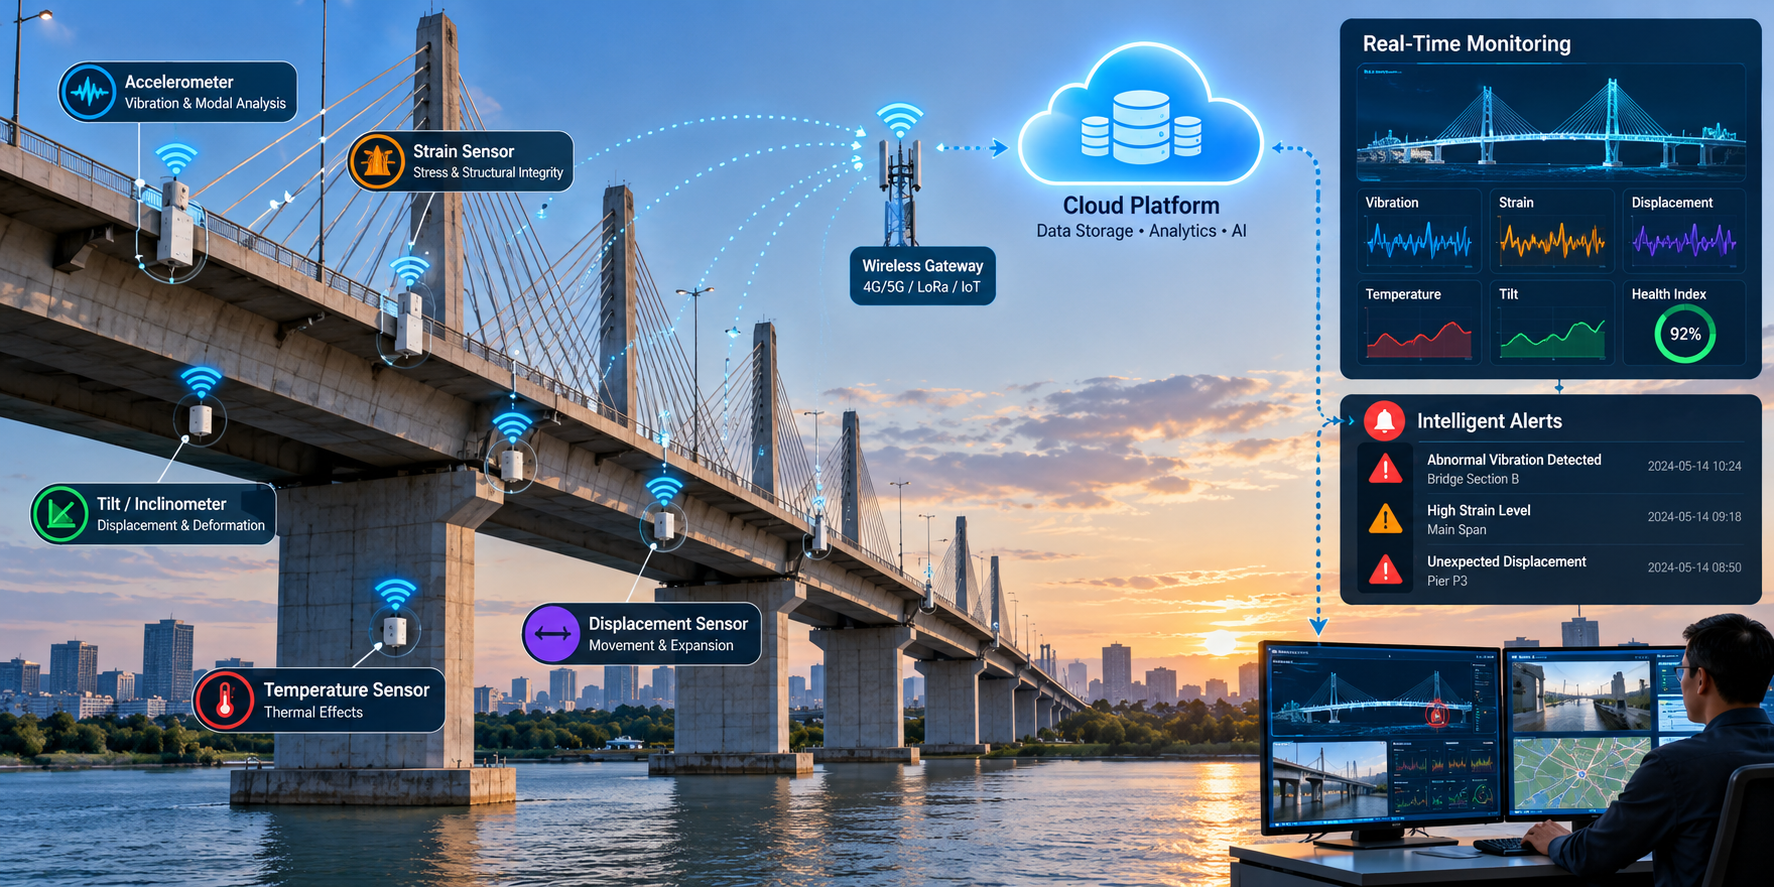
\includegraphics[width=\linewidth]{figures/ch11/ch11-02-v1-vague.png}};
\begin{scope}[x={(img.south east)},y={(img.north west)}]
  \tikzset{issuemark/.style={draw=Ch11IssueRed,line width=0.9pt,rounded corners=2pt,fill=white,fill opacity=0.90,text opacity=1,text=Ch11IssueRed,font=\sffamily\bfseries\scriptsize,inner sep=1.5pt}}
  \node[issuemark] at (0.35,0.62) {S1};
  \node[issuemark] at (0.24,0.82) {S2};
  \node[issuemark] at (0.55,0.84) {S3};
  \node[issuemark] at (0.95,0.64) {S4};
  \node[issuemark] at (0.78,0.44) {S5};
  \node[issuemark] at (0.64,0.76) {S6};
  \node[issuemark] at (0.62,0.28) {R1};
  \node[issuemark] at (0.64,0.91) {R2};
  \node[issuemark] at (0.11,0.56) {V1};
\end{scope}
\end{tikzpicture}
\caption{一句模糊提示词得到的初稿（反例）。编号对应表~\ref{tab:ch11-01} 的问题单：S1--S6 为科学错误，R1--R2 为阅读障碍，V1 为视觉一致性问题。科学错误超过三条时，修改单的第一项是重写输入，而不是修补这张图。底图由图像模型生成，其中文字为模型生成，未经核对。}\label{fig:ch11-02}
\end{figure}

\begin{table}[htbp]\centering\footnotesize
\setlength{\tabcolsep}{3pt}
\renewcommand{\arraystretch}{1.15}
\caption{将图~\ref{fig:ch11-02} 的“有点乱、不够专业”拆解为三层 9 条具体问题。}\label{tab:ch11-01}
\begin{tabularx}{\linewidth}{@{}c>{\raggedright\arraybackslash}p{17mm}>{\raggedright\arraybackslash}p{22mm}YY@{}}
\toprule
\textbf{编号} & \textbf{层级} & \textbf{位置} & \textbf{观察到的现象} & \textbf{为什么是问题} \\
\midrule
S1 & 科学错误 & 全桥构型 & 画成 6 塔三维透视斜拉桥，非双塔二维侧视图 & 与研究设定的双塔斜拉桥架构及立面工程制图不符 \\
S2 & 科学错误 & 桥上传感器 & 仅 5 个标签框；缺塔顶风速仪与 GNSS；应变计指在拉索上段而非主梁下缘；温度计放在桥墩下部 & 传感器类别不全、无法对应 12 个节点，布设部位违背工程常规 \\
S3 & 科学错误 & 网关至云平台 & 无线网关与云平台之间的蓝色虚线两端均带箭头 & 将单向汇聚上传监测数据画成了含义不明的双向箭头 \\
S4 & 科学错误 & 右上监控面板 & 凭空画出五条实时波形曲线及“Health Index 92\%”圆环 & 方法架构图不含实测数据，更无单一“92\% 健康评分”依据 \\
S5 & 科学错误 & 右中报警面板 & 写出 2024-05-14 的三条具体报警（B 段振动、主跨高应变、P3 墩位移） & 捏造了监测日期、墩号与结构异常事件 \\
S6 & 科学错误 & 全图文字框 & 英文标题、副标题、通信协议名与数值直接烧录在像素图中 & 文字属科学内容，锁死在位图中无法后期编校或改为中文 \\
R1 & 阅读障碍 & 背景与右下角 & 晚霞、城市天际线、江面反光与双屏操作员占据大半画幅 & 写实背景与装饰面板喧宾夺主，淹没传感与传输主干 \\
R2 & 阅读障碍 & 云平台内部 & 云朵内仅画数据库圆柱与“Data Storage $\cdot$ Analytics $\cdot$ AI” & 缺少“数据清洗 $\rightarrow$ 特征提取 $\rightarrow$ 阈值/异常判断”三步流程框 \\
V1 & 视觉一致性 & 传感器与标签 & 桥上节点全为同款白盒，说明框内却用蓝、橙、绿、红、紫五色圆图标 & 传感器本体无形状与颜色区分，不读文字无法按类型识别 \\
\bottomrule
\end{tabularx}
\end{table}

这张初稿仅第一层科学错误就有 6 条（S1--S6）。\textbf{当科学错误达到或超过三条时，修改单的第一条指令不是修补原图，而是退回任务书重写输入、重新生成。}

\section{修改单怎么写：一条只做一件事}

重新生成结构基准图（V2）前，先把系统构件、传感器数量与传输线定义为验收基准（表~\ref{tab:ch11-02}）。

\begin{table}[htbp]\centering\footnotesize
\setlength{\tabcolsep}{3pt}
\renewcommand{\arraystretch}{1.15}
\caption{斜拉桥结构健康监测系统示意图的对象表与关系表（V2 起的验收基准）。}\label{tab:ch11-02}
\begin{tabularx}{\linewidth}{@{}l>{\raggedright\arraybackslash}p{25mm}c>{\raggedright\arraybackslash}p{36mm}Y@{}}
\toprule
\textbf{编号} & \textbf{对象或关系} & \textbf{数量} & \textbf{位置（侧视图）} & \textbf{图形与线型约定（无字底图）} \\
\midrule
B1--B2 & 主梁与桥塔 & 1 梁 2 塔 & 左 $70\%$；塔在 $x\approx 0.22, 0.50$ & 浅灰扁长条主梁；中灰竖直单柱塔 \\
B3 & 斜拉索 & 16 & 每塔两侧各 4 根，扇形连塔上部与主梁 & 深灰细直线，全部连塔与梁，不入水不接地 \\
B4--B5 & 桥墩与水面 & 4 墩 1 水带 & 两塔下基础 + 两端边墩；底部水带 & 灰色墩座；浅蓝水面带 \\
S1--S5 & 加速度计 & $3+2$ & 主跨 $1/4, 1/2, 3/4$ 桥面（3）+ 两塔最长外索中部（2） & 蓝色小方块（每个传感器旁附 1 个黑点表示无线节点 N） \\
S6--S7 & 应变计 & 2 & 主跨跨中梁底、左塔旁梁底 & 绿色小矩形 \\
S8 / S9 & 风速仪 / GNSS & 各 1 & 左塔塔顶（S8）/ 右塔塔顶（S9） & 风杯形小图标 / 小圆盘天线图标 \\
S10 / S11--S12 & 温度计 / 位移计 & $1 / 2$ & 左边跨桥面（1）/ 两端伸缩缝（2） & 小圆形温度计图标 / 紫色小方块 \\
G / C / P / D & 网关/云/处理/终端 & 1/1/3/1 & 右 $30\%$ 数据路径区 & 右岸机柜加天线（G）；云内服务器条与三串联空框（C、P）；最右显示器加手机（D） \\
L1 & 无线传输 & 多条 & 各传感器节点 N $\rightarrow$ 网关 G & 橙色短虚线加小波纹，必须与斜拉索明显不同 \\
L2 / L3 / L4 & 上传 / 处理 / 预警 & 1 / 2 / 1 & G$\rightarrow$C / P 三框间 / P 末框$\rightarrow$D & 橙色实线箭头 / 深灰小箭头 / 红色实线箭头（全图唯一红色） \\
\bottomrule
\end{tabularx}
\end{table}

在 \scidraw{} 科研绘图向导（\sdtool{figure-workflow}）中选择“机制与流程图”路线，把模板替换为以下任务书并下载保存，再到流程图入口（\sdtool{workflow-diagram-generator}）或提示词绘图（\sdtool{ai-drawing}）生成：

\begin{Prompt}
【用途与读者】硕士论文第 2 章方法部分的系统示意图；印刷宽度约 160 mm（单页通栏），
读者为土木与结构工程同行。
【目标】让读者看清：传感器布设在桥的哪些部位、测什么；数据如何经无线节点到
现场网关、再上传云端分析；预警如何送达管理人员。
【材料】Farrar & Worden 2007；Ko & Ni 2005；Lynch & Loh 2006。本图为教学用简化架构，
不对应某座真实桥梁，不含任何监测数据。
【对象】见对象表 B1–B5、S1–S12、G、C、P、D；斜拉索每塔每侧 4 根，共 16 根；
传感器共 12 个，同类传感器同形同色。
【关系】L1 无线传输：橙色短虚线带小波纹，从各传感器到网关，不得与斜拉索相似；
L2 网关→云：橙色实线箭头；L3 云内三步处理：深灰小箭头；L4 判断→终端：红色箭头，
全图唯一红色。
【布局】横向 2:1。左 70% 为桥的侧视图（水面在下），右 30% 自下而上为网关、云、
终端；数据从左到右、自下而上流动。底部 10% 留给图例。
【视觉】白底，扁平二维工程示意风格，无渐变、无阴影、无 3D；结构灰阶，传感器用蓝/绿/紫。
【限制】底图不含任何文字、字母、数字；不画车辆、行人、城市、数据曲线、裂缝、主缆；
不画从云到传感器或从传感器到终端的直接箭头。
【验收】双塔斜拉桥；拉索 16 根连塔与梁；12 个传感器位置与类型正确；L1–L4 方向正确；
无线虚线与拉索可区分；底图无文字；160 mm 宽时图标可辨。
\end{Prompt}

转为结构化英文提示词提交生成（完整提示词见本书仓库 \texttt{cases/} 目录，关键段落如下）：

\begin{Prompt}
Flat 2D engineering schematic, landscape 2:1, pure white background, clean vector
style, flat fills, thin dark gray outlines, no gradients, no shadows, no 3D.
ABSOLUTELY NO TEXT: no letters, words, numbers, symbols, labels, legend or title.
LEFT 70% - SIDE VIEW OF A TWIN-PYLON CABLE-STAYED BRIDGE (no main cable, no hangers):
- Pale blue water band (y 0.75-0.88); light gray deck girder (x 0.03-0.68, y 0.60-0.63);
  two medium gray vertical pylons at x 0.22 and x 0.50 on gray piers; two end piers.
- Exactly 16 straight thin dark gray stay cables: 4 left and 4 right on each pylon,
  every cable connecting pylon to deck, none touching water or ground.
- SENSORS (12 total, each with a tiny black wireless node dot beside it):
  3 blue squares on main-span deck (1/4, 1/2, 3/4); 2 blue squares on longest outer
  cables; 2 green rectangles under deck; 1 cup anemometer on left pylon top; 1 dish
  GNSS antenna on right pylon top; 1 round thermometer on left side span; 2 purple
  squares at both deck ends.
RIGHT 30% - DATA PATH: gateway cabinet with antenna on right bank; cloud outline with
3 server bars and 3 empty rounded processing boxes connected by dark gray arrows;
operator terminal (monitor + phone) at far right.
LINES: short orange dashed wireless lines with wave marks from sensors to gateway;
one solid orange upload arrow (gateway -> cloud); one solid red alert arrow (last box
-> terminal; red used nowhere else). Keep bottom 10% empty for legend.
\end{Prompt}

把同一英文提示词连续生成三次，每次放大到 $200\%$ 对照表~\ref{tab:ch11-02} 清点：第 1 次生成中，每塔每侧连到塔身的拉索只有 $3+3+3+3=12$ 根，左外侧蓝色传感器附着在一段上端悬空的孤立斜线上，淘汰；第 3 次生成虽有 16 条拉索走向和 12 个传感器，但主跨拉索交叉拥挤，左塔顶风速仪被涂成与加速度计相同的蓝色，网关悬空且云压入水面带，淘汰；第 2 次生成（图~\ref{fig:ch11-03}）具备双塔侧视、16 条连接塔与主梁的拉索走向、全部 12 个传感器及旁侧黑点、网关/云/处理框/终端与四类箭头的正确方向，且全图零文字，选作后续比较的\textbf{候选结构基准（V2）}。

\begin{figure}[htbp]\centering
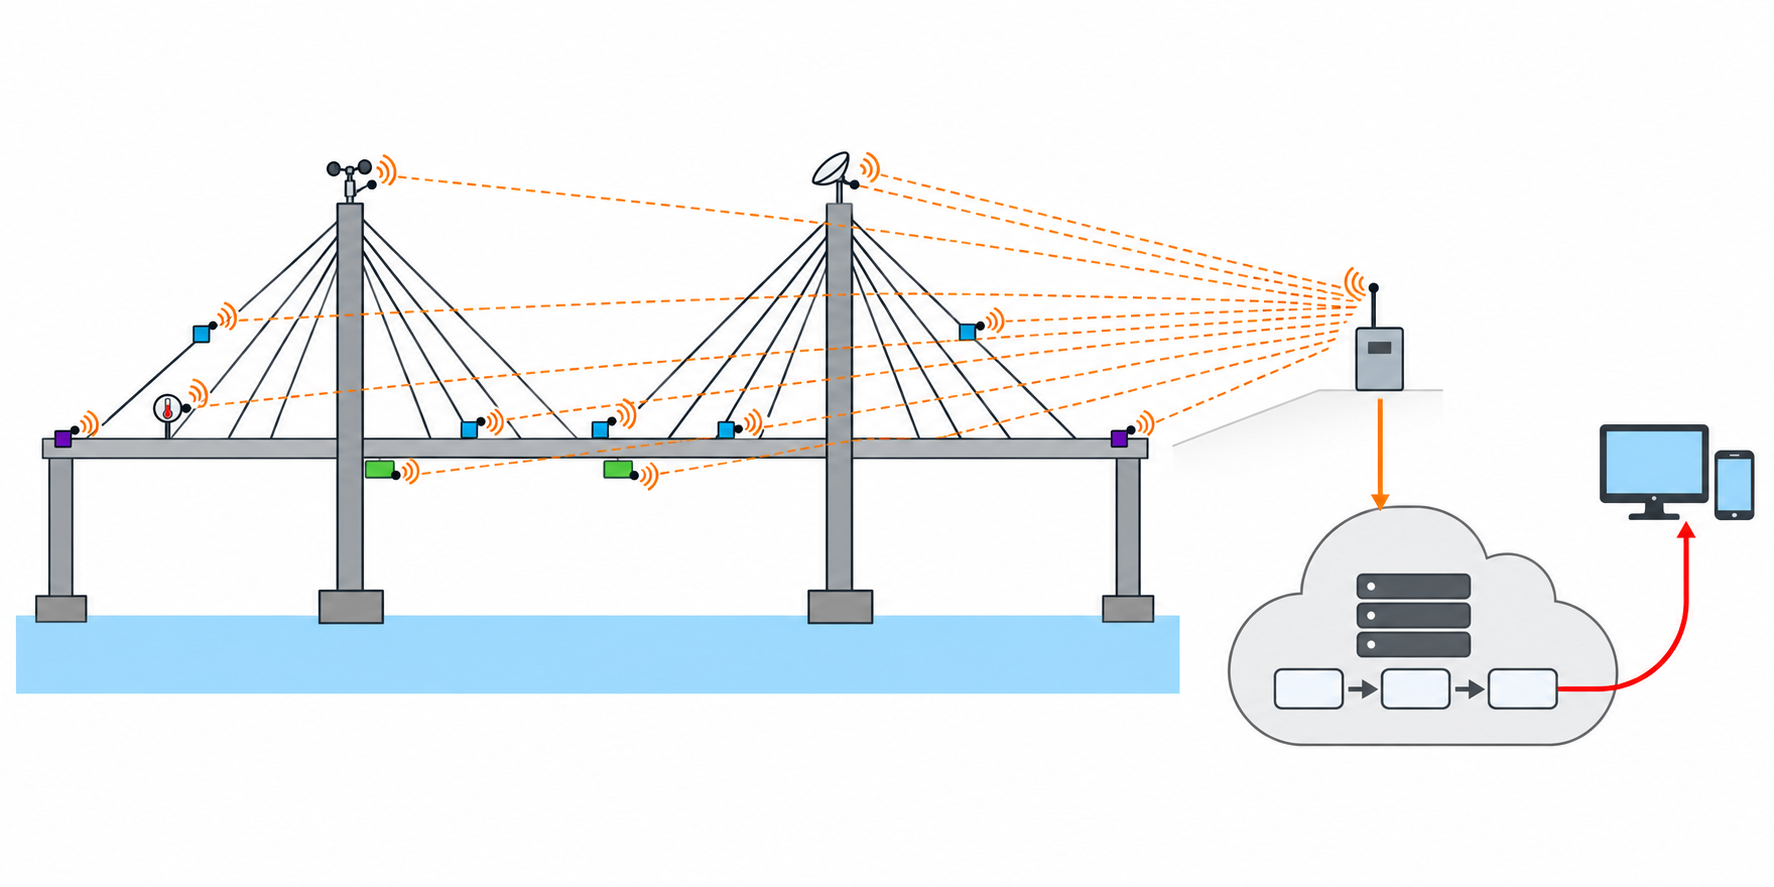
\includegraphics[width=\linewidth]{figures/ch11/ch11-03-v2-brief.png}
\caption{按完整任务书生成的候选结构基准 V2（第 2 次生成结果）。桥型、16 条斜拉索走向、12 个传感器、右侧子系统与数据流语义方向符合表~\ref{tab:ch11-02}，全图无文字，作为后续所有版本比较的参考基准；但仍留有无线虚线偏细、云在网关下方、温度计内部带红色、图标偏小及拉索局部白隙等缺陷（见表~\ref{tab:ch11-03} 修改单）。底图由图像模型生成。}\label{fig:ch11-03}
\end{figure}

V2 只是比较基准而非验收通过的终稿。对照任务书对其全面体检，即可写出结构化\textbf{修改单}（表~\ref{tab:ch11-03}）。每条修改单包含编号、层级、位置、实测现象、修改要求、**必须保持不变的内容**、核对方法与执行通道。

\begin{table}[htbp]\centering\footnotesize
\setlength{\tabcolsep}{3pt}
\renewcommand{\arraystretch}{1.15}
\caption{针对候选基准 V2（图~\ref{fig:ch11-03}）实测问题编写的修改单。}\label{tab:ch11-03}
\begin{tabularx}{\linewidth}{@{}c>{\raggedright\arraybackslash}p{14mm}>{\raggedright\arraybackslash}p{18mm}YYY>{\raggedright\arraybackslash}p{18mm}@{}}
\toprule
\textbf{ID} & \textbf{层级} & \textbf{位置} & \textbf{实测现象与影响} & \textbf{修改要求} & \textbf{必须保持不变} & \textbf{执行通道} \\
\midrule
R2 & 阅读障碍 & 传感器至网关线 & 橙色无线虚线偏细，横穿拉索扇面时区分度不足 & 改为更粗的橙色短虚线并带波纹，与深灰细实线拉索明显不同 & 桥型、16 条拉索、12 个传感器、网关/云/终端及 L2--L4 & 生成模型（参考图修改）；失败两次则改用 TikZ \\
R3 & 阅读障碍 & 全部传感器 & $160\ \text{mm}$ 宽下蓝方块约 $1.44\text{--}1.80\ \text{mm}$，小于 $2\ \text{mm}$ & 传感器图标放大约 $1.5$ 倍（与 R2 分开独立执行） & 同上全部结构与连接线 & 生成模型（独立轮次）或排版层覆盖 \\
R4 & 阅读障碍 & 右侧数据路径 & 网关在上方（$y\approx 0.41$）、云在下方（$y\approx 0.71$），上传箭头朝下，路径折返 & 教学稿按实测位置叠字说明；正式投稿需对调网关与云的上下位置 & 左 $70\%$ 桥体、16 根拉索与 12 个传感器不变 & 排版层适配坐标或重生成右侧 \\
V1 & 视觉一致性 & 温度计与蓝方块 & 温度计含红色液柱，违反“红色仅用于预警”；蓝方块色值未精确统一 & 温度计去红改灰；同类加速度计统一色值（如 \texttt{\#4C78A8}） & 其余传感器、结构灰阶与红预警箭头 & 后期图像/排版层修色 \\
V2 & 视觉一致性 & 拉索交界与水面 & 部分拉索穿过图标和波纹处有白色断开窄隙；水面与屏幕带渐变 & 正式发表前在矢量或图像软件中补连拉索断口、平涂渐变区 & 16 条拉索端点与传感器坐标 & 排版层 / 矢量软件 \\
T1 & 文字与图例 & 全图与底边 & 底图无文字，需构件名、子系统名与图例 & 在 LaTeX/TikZ 中按实测坐标叠加 7 处标签与底部图例 & 底图像素不动 & 排版层（TikZ） \\
\bottomrule
\end{tabularx}
\end{table}

\begin{BookNote}
\textbf{修改单的三条规则：}（1）\textbf{一次只改一类问题}，不把加粗虚线、放大图标、对调位置塞进同一条生成指令；（2）\textbf{必须写明“保持不变”清单}，用具体对象和数量取代笼统的“其余不变”；（3）\textbf{文字、精确色值、断口补线与对齐优先在排版层完成}，不靠生成模型反复重绘。
\end{BookNote}

\section{局部指令的连带变化：怎么发现它}

为什么修改单如此谨慎地限制生成模型修改？因为图像生成模型的“局部修改”并不是在原图图层上擦改一根线，而是以参考图和提示词为条件**重新合成整张画布**。在 \scidraw{} 绘图（\sdtool{ai-drawing}）中选择历史图作为参考图修改时，同样没有“对象锁定”或“区域像素冻结”，模型可能顺手改动未提及的对象——即发生\textbf{连带变化（collateral changes）}。

\subsection{真实例子一：第 7 章只要求统一风格，却改坏了五处结构}

先看本书第 7 章胰岛素促进 GLUT4 转位机制图的真实迭代记录（图~\ref{fig:ch11-07}）。其 V2 基准图（图~\ref{fig:ch11-07}左）已画对 13 个对象、6 枚琥珀色磷酸化圆点及五类线型。进入 V3 时，作者只要求统一蛋白蓝色色值、统一线宽并增加留白，提示词写明“保持相同内容与布局”。

然而，当第 1 次生成未传入 V2 参考图、仅凭修订提示词重新生成时（图~\ref{fig:ch11-07}中），虽然配色和线条变得干净，却出现了五处严重的结构连带变化：(a) 受体、IRS-1、Akt 和 AS160 上的 6 枚磷酸化圆点全部丢失；(b) 胰岛素由 3 珠减为 2 珠且脱离受体；(c) 原本紧贴质膜内叶的 PDK1 与 Akt 脱离质膜掉入胞质；(d) PI3K 与 PDK1 之间多出一条未经授权的实心激活箭头；(e) 每个囊泡上的 GLUT4 由 1 个变为多个，胞内还多出葡萄糖六边形。直到第 2 次将 V2 作为参考图传入（图~\ref{fig:ch11-07}右），才保住了主要结构与磷酸化圆点。即便传入参考图，第 7 章做配色反例实验时，模型仍在重绘中把 $\text{PIP}_2 \rightarrow \text{PIP}_3$ 转化弧的空心箭头悄悄改成了实心箭头。

\begin{figure}[htbp]\centering
% FIG ch11-07 Chapter 7 collateral reuse (Chinese)
\usetikzlibrary{arrows.meta,calc}
\begin{tikzpicture}
  \def\panelW{0.31\linewidth}
  \definecolor{Ch11AnnotRed}{HTML}{C0392B}
  \node[anchor=south west, inner sep=0] (imA) at (0,0) {%
    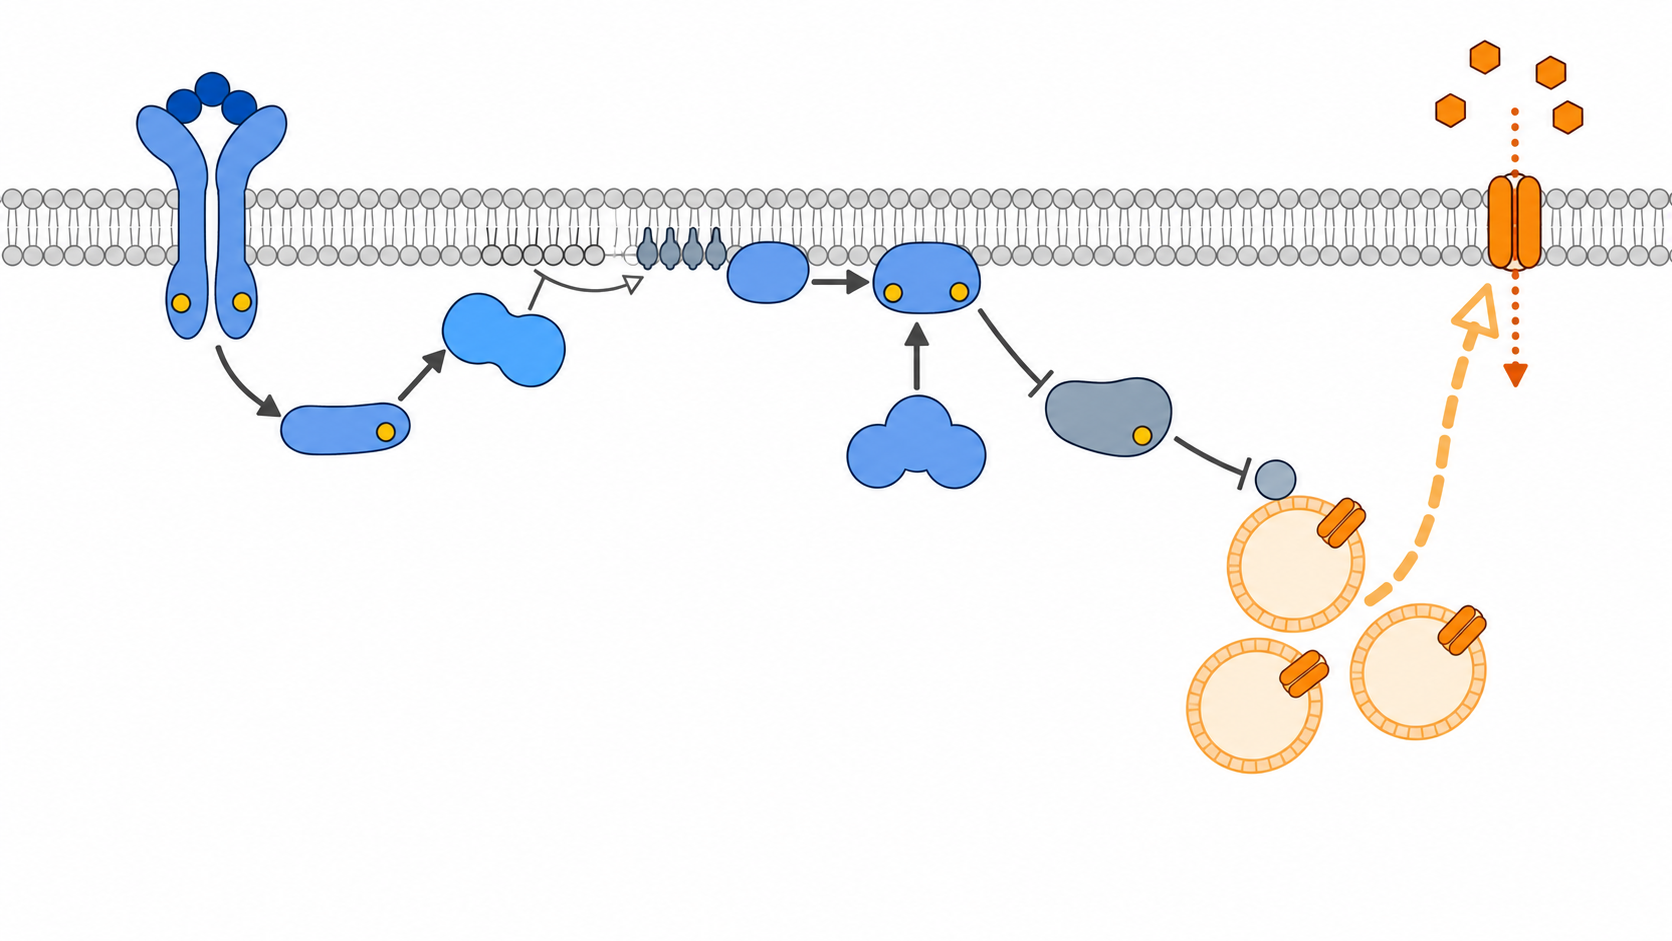
\includegraphics[width=\panelW]{figures/ch11/ch11-07a-ch07-v2.png}};
  \node[font=\small\sffamily, anchor=south] at ($(imA.north)+(0,2mm)$) {V2 基准};

  \node[anchor=south west, inner sep=0] (imB) at (0.345\linewidth,0) {%
    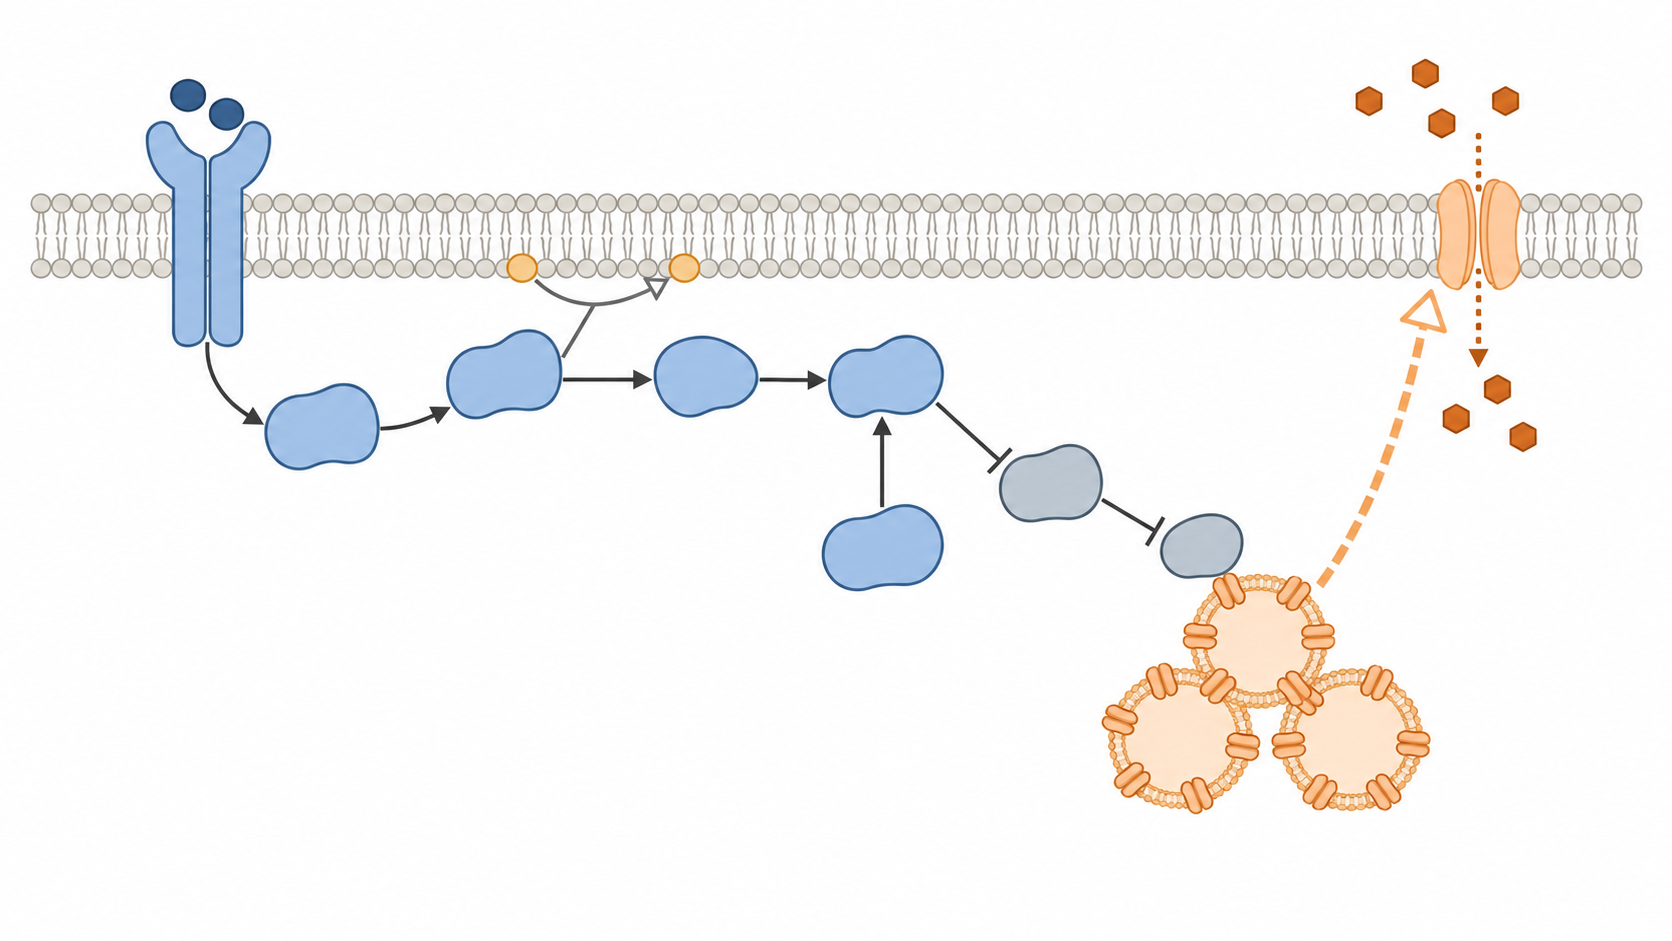
\includegraphics[width=\panelW]{figures/ch11/ch11-07b-ch07-v3-alt1.png}};
  \node[font=\small\sffamily, anchor=south] at ($(imB.north)+(0,2mm)$) {V3 第 1 次（不采用）};
  \begin{scope}[x={(imB.south east)},y={(imB.north west)}]
    \draw[Ch11AnnotRed, line width=0.7pt] (0.11,0.28) circle (0.035);
    \node[font=\scriptsize\sffamily, text=Ch11AnnotRed, anchor=west] at (0.15,0.28) {(a)};
    \draw[Ch11AnnotRed, line width=0.7pt] (0.10,0.08) circle (0.04);
    \node[font=\scriptsize\sffamily, text=Ch11AnnotRed, anchor=west] at (0.14,0.08) {(b)};
    \draw[Ch11AnnotRed, line width=0.7pt] (0.48,0.38) circle (0.06);
    \node[font=\scriptsize\sffamily, text=Ch11AnnotRed, anchor=west] at (0.54,0.38) {(c)};
    \draw[Ch11AnnotRed, line width=0.7pt] (0.34,0.36) circle (0.045);
    \node[font=\scriptsize\sffamily, text=Ch11AnnotRed, anchor=west] at (0.39,0.36) {(d)};
    \draw[Ch11AnnotRed, line width=0.7pt] (0.76,0.70) circle (0.07);
    \node[font=\scriptsize\sffamily, text=Ch11AnnotRed, anchor=west] at (0.82,0.70) {(e)};
  \end{scope}

  \node[anchor=south west, inner sep=0] (imC) at (0.69\linewidth,0) {%
    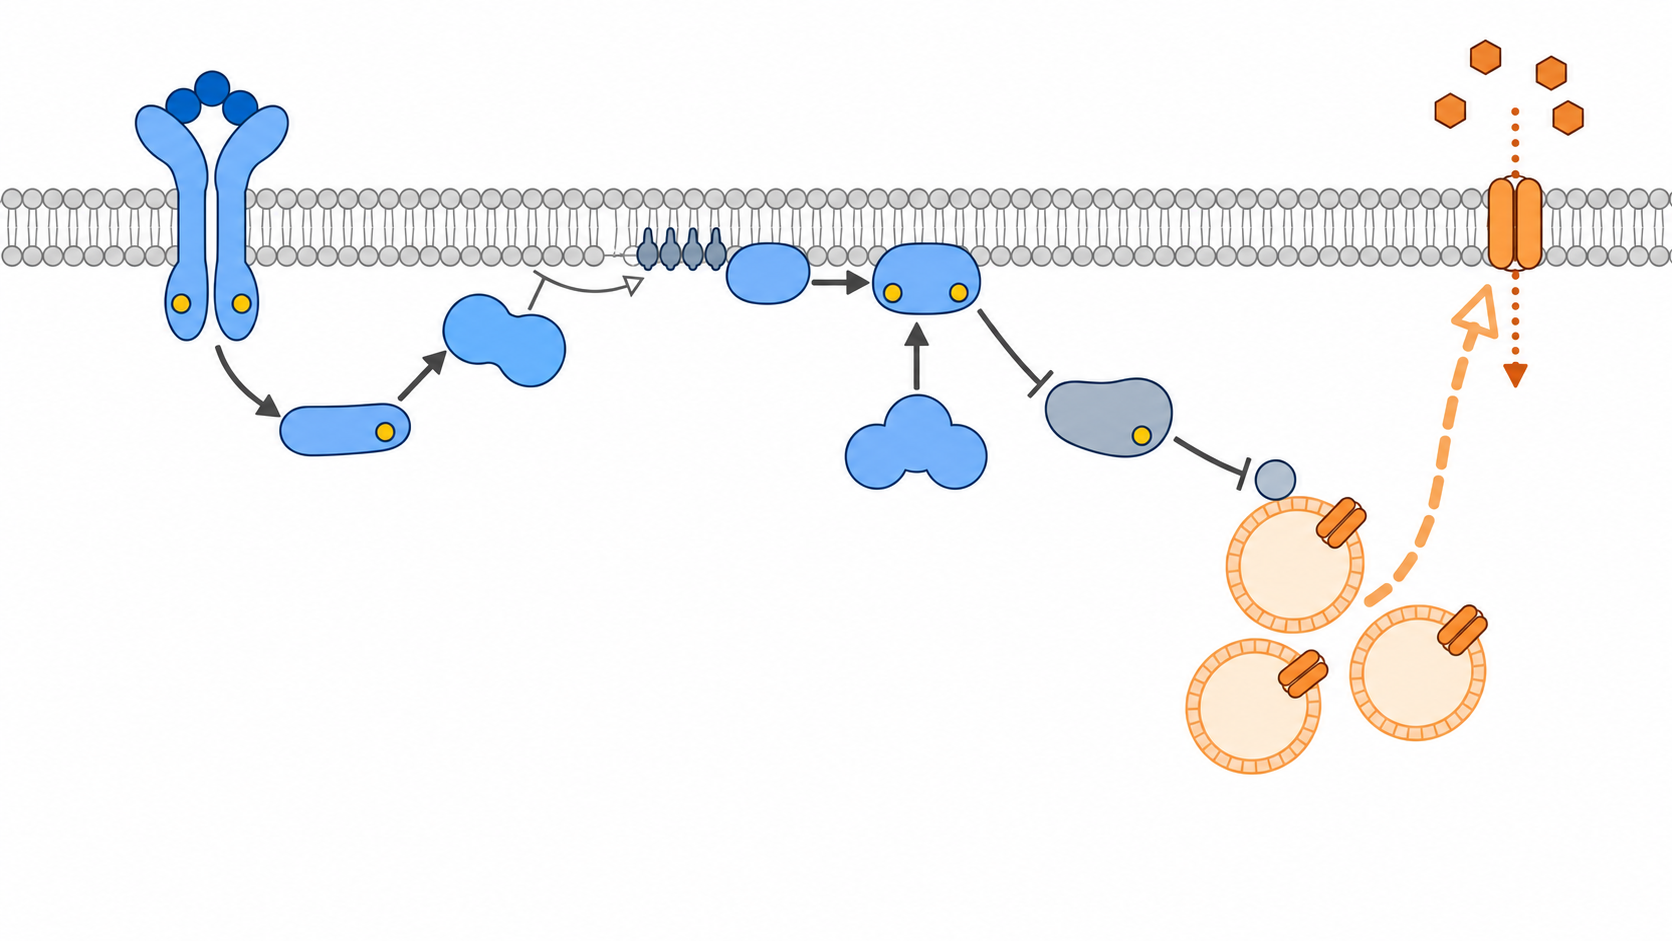
\includegraphics[width=\panelW]{figures/ch11/ch11-07c-ch07-v3.png}};
  \node[font=\small\sffamily, anchor=south] at ($(imC.north)+(0,2mm)$) {V3 第 2 次（采用）};
\end{tikzpicture}

\caption{第 7 章的真实迭代：关于配色与线型的修订提示词也可能改动结构。左为 V2 基准；中为同一修订提示词第 1 次生成（未传参考图）：(a) 磷酸化标记全部丢失，(b) 胰岛素由三珠变两珠且脱离受体，(c) PDK1 与 Akt 离开质膜，(d) 新增未要求的 PI3K$\rightarrow$PDK1 激活箭头，(e) 每个囊泡上的 GLUT4 由一个变为多个；右为传入 V2 作参考图的第 2 次生成，主要结构保留，但仍需整图复核。三图均由图像模型生成。}\label{fig:ch11-07}
\end{figure}

\subsection{真实例子二：本章 V3 参考图修改的三次实测}

再看本章修改单第一项（R2）。在 \scidraw{} 绘图中从历史记录选择 V2（图~\ref{fig:ch11-03}）作为参考图，输入只改无线传输线的指令：

\begin{Prompt}
把所有从传感器到网关的无线传输线改为更粗的橙色短虚线，并在线上加小波纹，
让它们与斜拉索一眼就能区分。其他内容保持不变。
\end{Prompt}

实际提交的英文指令为：

\begin{Prompt}
Using the reference image, change only the wireless lines from the sensors to
the gateway: make them thicker orange short-dashed lines with small wave marks,
so they cannot be confused with the stay cables. Keep everything else
unchanged. No text.
\end{Prompt}

我们独立以 V2 为参考图连续执行了三次修改，每次都按表~\ref{tab:ch11-02} 清点全部对象。图~\ref{fig:ch11-04} 将 V2（左）与 V3 第 1 次结果（右）并排对比。

\begin{figure}[htbp]\centering
\resizebox{\linewidth}{!}{%
\begin{tikzpicture}
\definecolor{Ch11OkGreen}{HTML}{2E8B57}
\definecolor{Ch11WarnRed}{HTML}{C0392B}
\node[anchor=south west,inner sep=0] (imL) at (0,0) {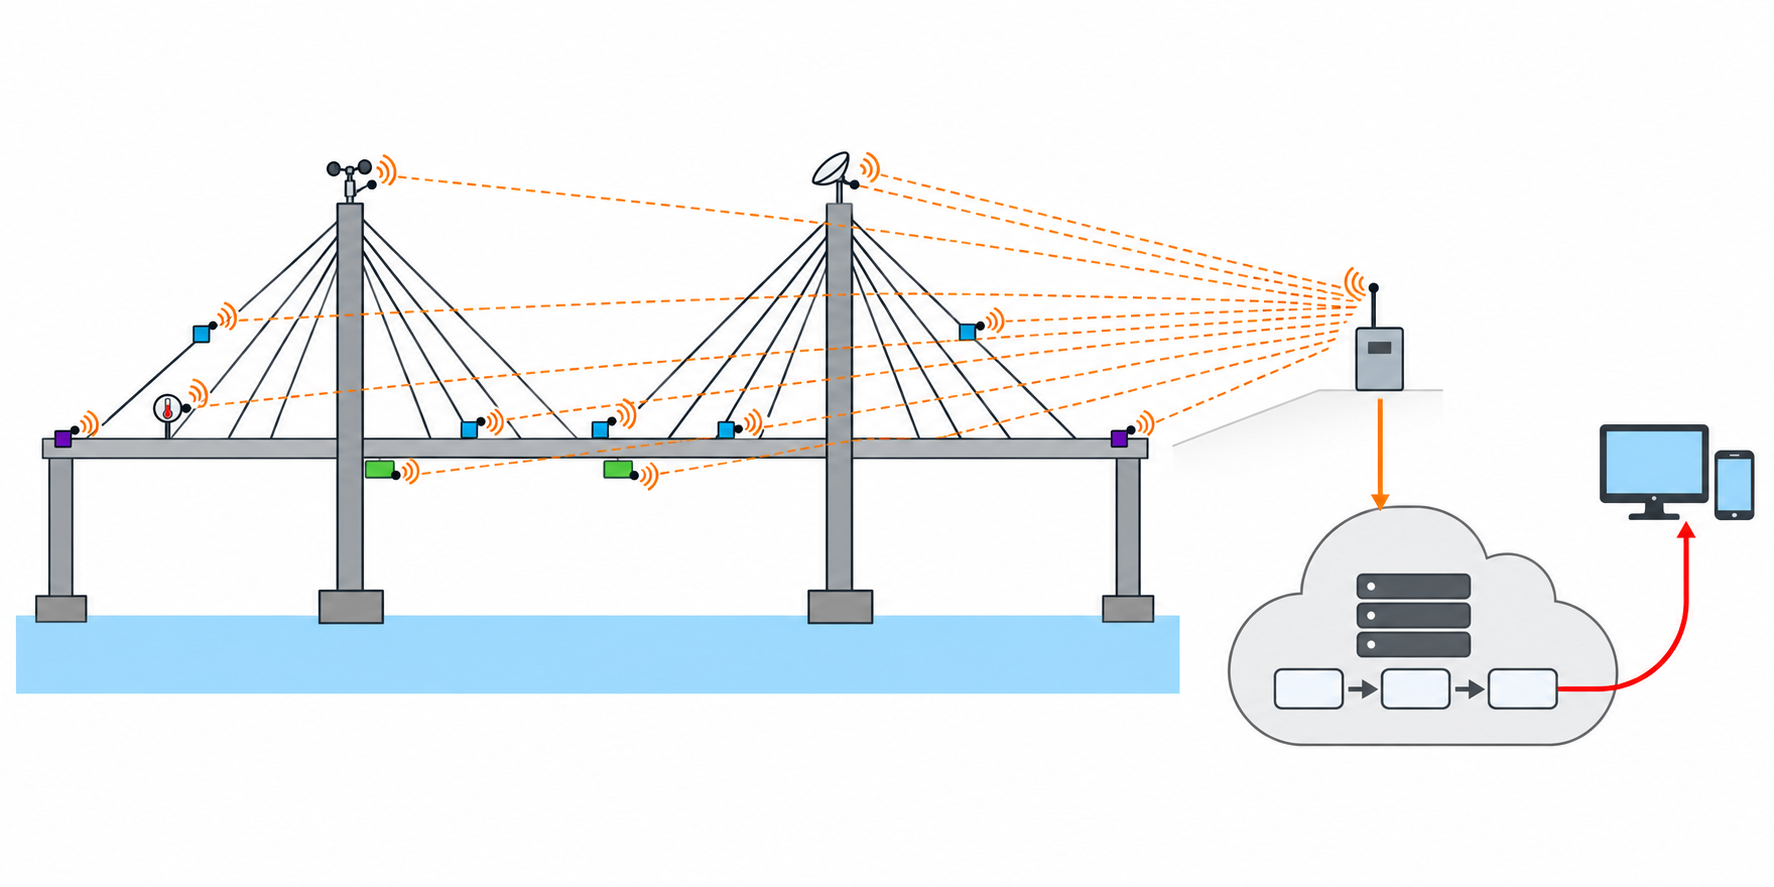
\includegraphics[width=0.488\linewidth]{figures/ch11/ch11-03-v2-brief.png}};
\node[font=\sffamily\footnotesize,anchor=south] at ($(imL.north)+(0,1.5mm)$) {V2 候选基准（修改前）};
\node[anchor=south west,inner sep=0] (imR) at (0.512\linewidth,0) {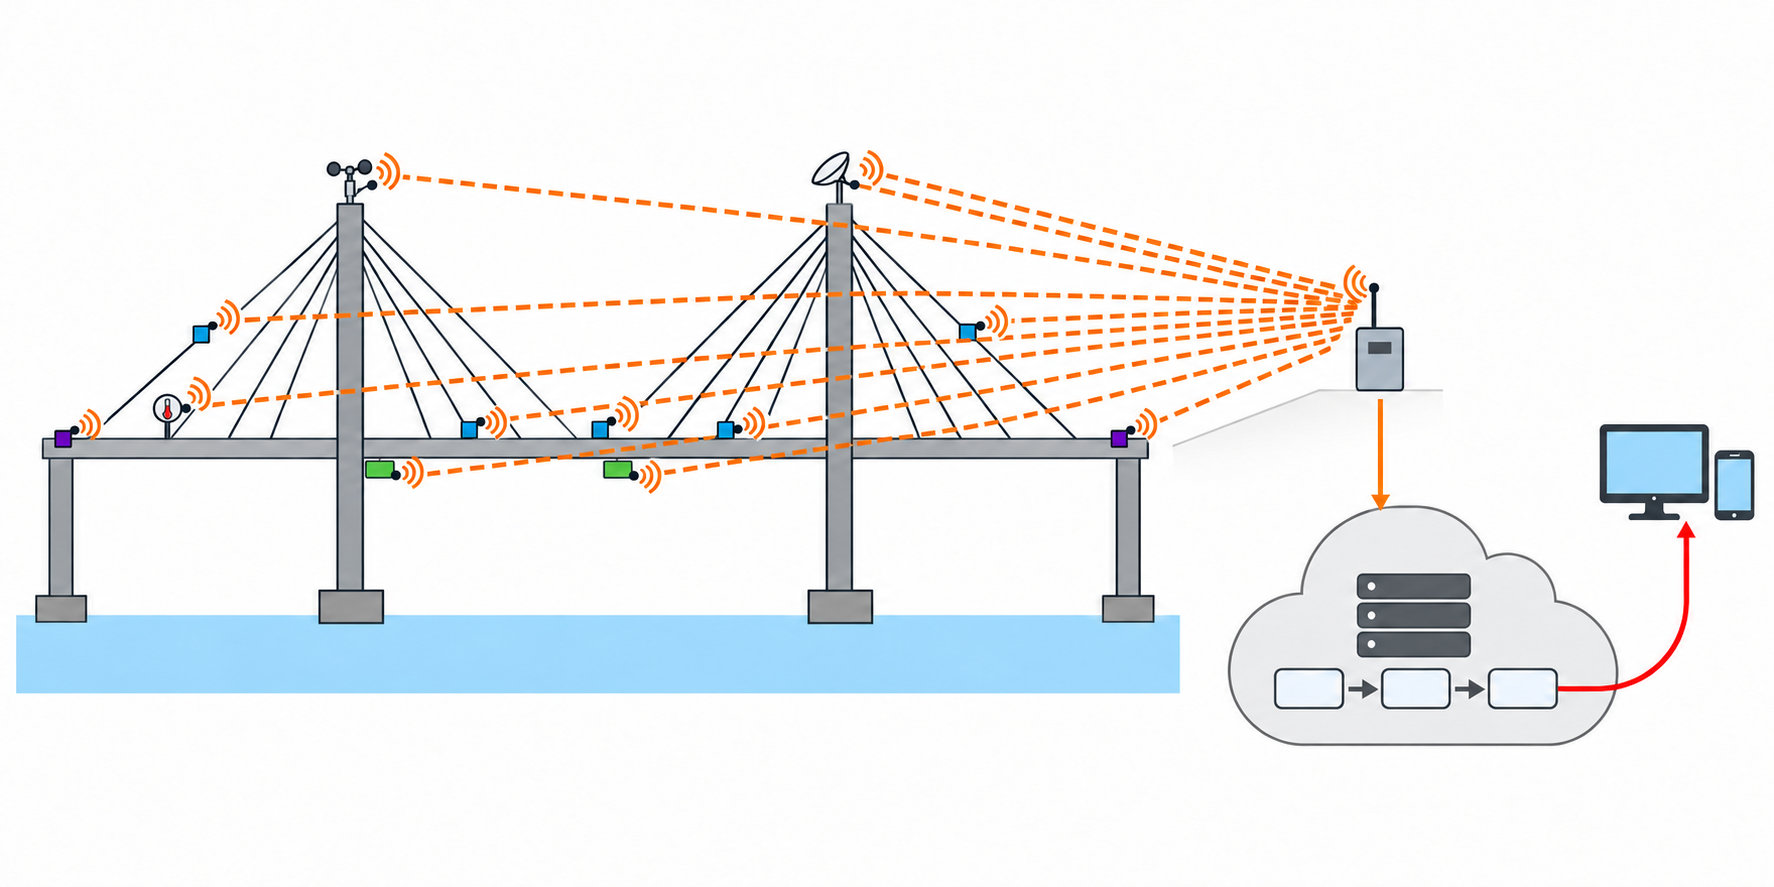
\includegraphics[width=0.488\linewidth]{figures/ch11/ch11-04-v3-collateral.png}};
\node[font=\sffamily\footnotesize,anchor=south] at ($(imR.north)+(0,1.5mm)$) {V3 第 1 次（参考图局部修改后）};
\begin{scope}[x={(imR.south east)},y={(imR.north west)}]
  \draw[Ch11OkGreen,line width=0.9pt,rounded corners=2pt] (0.50,0.61) rectangle (0.76,0.80);
  \node[fill=white,fill opacity=0.9,text opacity=1,text=Ch11OkGreen,font=\sffamily\bfseries\scriptsize,inner sep=1pt,anchor=south] at (0.63,0.81) {目标修改完成：橙虚线加粗};
  \draw[Ch11WarnRed,dashed,line width=0.7pt,rounded corners=2pt] (0.06,0.49) rectangle (0.13,0.59);
  \node[fill=white,fill opacity=0.9,text opacity=1,text=Ch11WarnRed,font=\sffamily\scriptsize,inner sep=1pt,anchor=south] at (0.10,0.60) {继承偏差 1};
  \draw[Ch11WarnRed,dashed,line width=0.7pt,rounded corners=2pt] (0.68,0.14) rectangle (0.91,0.44);
  \node[fill=white,fill opacity=0.9,text opacity=1,text=Ch11WarnRed,font=\sffamily\scriptsize,inner sep=1pt,anchor=north] at (0.80,0.13) {继承偏差 2：云仍在网关下方};
\end{scope}
\end{tikzpicture}}
\caption{只要求修改无线传输线后得到的 V3 第 1 次结果（右），与候选基准 V2（左）并排。绿色实线框标出已完成的目标修改（橙色短虚线加粗、波纹更醒目）；三次独立参考图修改均保住了 16 条斜拉索走向与 12 个传感器，未观察到明显结构连带变化，但仍需整图复核。红色虚线框标出从 V2 原样继承的既有偏差（温度计带红色、云在网关下方）。底图均由图像模型生成，未经人工改动。}\label{fig:ch11-04}
\end{figure}

三次实测给出了三点结论：（1）\textbf{目标修改完成}：三次尝试都把橙色短虚线明显加粗、节点旁波纹更醒目，与深灰细实线拉索清楚区分（但波纹仍集中在节点旁，未遍布链路中段）；（2）\textbf{三次尝试均未出现少索、少传感器或网关移位等结构连带变化}：2 座桥塔、16 条拉索走向、12 个传感器（$3+2+2+1+1+1+2$）和右侧网关、云、3 个处理框、终端及箭头全部保持一致；（3）\textbf{V2 原有缺陷被原样继承}：温度计带红（继承偏差 1）、云在网关下方（继承偏差 2）、小图标与拉索局部白隙在三次结果中依然存在。

这说明连带变化具有随机性：**“本次没有发生结构连带变化”只能在逐项清点后得出，绝不能在清点前假定。**

\subsection{用并排比较、像素差异图与对象计数表核验}

排查连带变化可结合三种方法（图~\ref{fig:ch11-05}）：

\begin{figure}[htbp]\centering
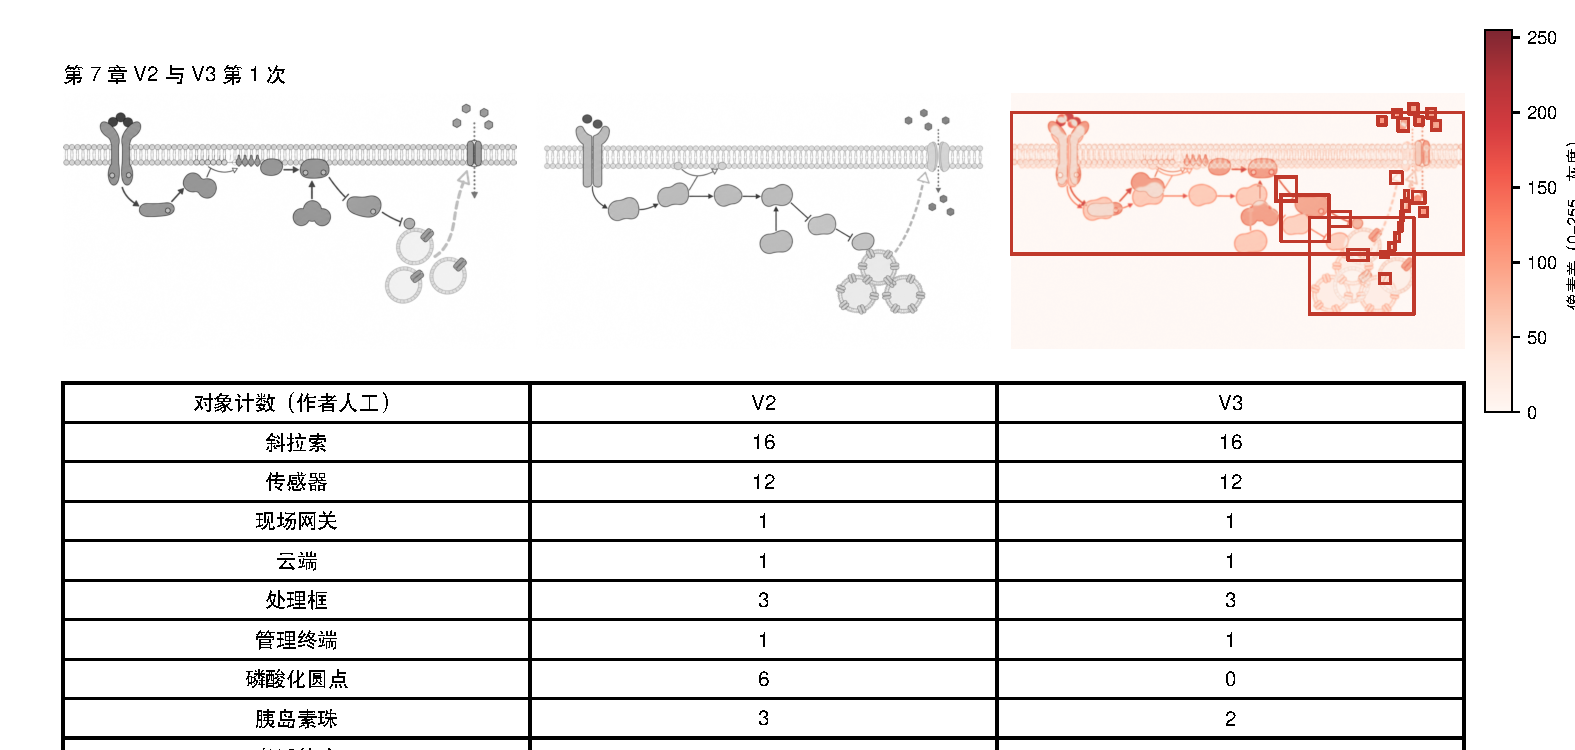
\includegraphics[width=\linewidth]{figures/ch11/ch11-05-diff-and-count-zh.pdf}
\caption{用差异图和对象计数发现连带变化。差异图显示两版之间灰度像素变化的位置；构图基本不变时，它能直接指出变动区；整张图被重排重绘时（上排：第 7 章 V2 与 V3 第 1 次尝试），差异红框遍布全图（共 24 个区域），此时只能依靠按对象表逐项计数（下表：前 6 行为本章 V2 与 V3 计数，后 4 行为第 7 章计数）。计数由作者人工完成。}\label{fig:ch11-05}
\end{figure}

第一，\textbf{同尺寸并排比较或叠放切换}。\scidraw{} 当前未内置版本并排对比视图，需将新旧两版下载后同宽并排（如图~\ref{fig:ch11-04}）或在看图软件中快速前后切换，靠视觉闪烁发现未修改区的位移。

第二，\textbf{像素差异热图及其局限}。将两图缩放到同尺寸转灰度（$0\text{--}255$），计算逐像素绝对差，经高斯模糊（半径约 2 像素）抑制抗锯齿噪点后，圈出灰度差大于 40 的连通域。当构图保持不变时，热图能直接指出变动线条；但当模型重排了全图构图时——如图~\ref{fig:ch11-05} 上排的第 7 章 V2 与 V3 第 1 次尝试——全图约 $14.6\%$ 的像素超阈值，24 个红框覆盖全图，失去定位能力。

第三，\textbf{人工对象计数表（最终防线）}。对照对象表逐项清点（图~\ref{fig:ch11-05} 下表）：本章 V2 与 V3 的斜拉索（16/16）、传感器（12/12）、网关（1/1）、云端（1/1）、处理框（3/3）、管理终端（1/1）完全一致；而第 7 章 V2 与 V3 第 1 次尝试中，磷酸化圆点由 6 变 0、胰岛素珠由 3 变 2、激活箭头由 4 变 5、每囊泡最大 GLUT4 由 1 变 3。像素差异图只作辅助，人工按表计数才能把住科学关。

\section{回到上一版再改，以及何时换走排版层}

一旦在某次修改中发现了连带变化（如丢了天线或少了拉索），绝不能在出错的 V3 上继续输入“把消失的天线加回来”。正如图~\ref{fig:ch11-08} 右下虚线框所示，在错误版本上叠加修改（$\text{V3} \rightarrow \text{V3}' \rightarrow \text{V3}''$）会让每次全图重绘引入新变形，错误层层累积且无法追溯。

\begin{figure}[htbp]\centering
\resizebox{\linewidth}{!}{\tikzset{every node/.append style={align=center}}% FIG ch11-08 version tree (Chinese)
\usetikzlibrary{arrows.meta,positioning,fit,calc}
\definecolor{Ch11BadRed}{HTML}{C0392B}
\definecolor{Ch11GoodGreen}{HTML}{2E8B57}
\providecommand{\ChElevenThumb}[2]{%
  \IfFileExists{#1}{%
    \includegraphics[width=24mm]{#1}%
  }{%
    \fbox{\parbox[c][16mm][c]{24mm}{\centering\scriptsize\sffamily #2\\{\tiny （底图待出）}}}}%
}
\begin{tikzpicture}[
  x=1mm, y=1mm,
  font=\sffamily\footnotesize,
  edge/.style={draw=BookInk!60, -{Stealth[length=2mm]}, line width=0.55pt},
  badedge/.style={draw=Ch11BadRed!70, dashed, -{Stealth[length=2mm]}},
  nlabel/.style={align=center, text width=26mm, font=\scriptsize},
]
  \node (V1) at (0,0) {\ChElevenThumb{figures/ch11/ch11-02-v1-vague.png}{V1}};
  \node[nlabel, below=1mm of V1] {模糊提示词};

  \node (V2) [below=14mm of V1] {\ChElevenThumb{figures/ch11/ch11-03-v2-brief.png}{V2\\基准}};
  \node[nlabel, below=1mm of V2] {\textbf{结构基准}};

  \node (V3) [below=14mm of V2] {\ChElevenThumb{figures/ch11/ch11-04-v3-collateral.png}{V3}};
  \node[nlabel, below=1mm of V3, text=Ch11BadRed] {连带变化\\{\tiny（不采用）}};

  \node (V4) at (42,-28) {\ChElevenThumb{figures/ch11/ch11-06-v4-recovered.png}{V4}};
  \node[nlabel, below=1mm of V4, text=Ch11GoodGreen] {回到 V2\\只改无线线};

  \node (Final) at (84,-28) {\ChElevenThumb{figures/ch11/ch11-06-v4-recovered.png}{终稿}};
  \node[nlabel, below=1mm of Final] {TikZ 标签与图例};

  \draw[edge] (V1) -- node[left, font=\tiny, align=right] {重写\\输入} (V2);
  \draw[edge] (V2) -- node[right=1.5mm, font=\tiny, align=left] {只改\\无线线} (V3);
  \draw[edge] (V2.east) -- node[above, font=\tiny] {只改无线线\\+ 保留清单} (V4.west);
  \draw[edge] (V4.east) -- node[above, font=\tiny] {叠加标签\\与图例} (Final.west);

  \node[draw=Ch11BadRed, dashed, rounded corners=2pt, inner sep=4pt, fit=(V3)] {};
  \node[font=\scriptsize, text=Ch11BadRed, right=1mm of V3] {×};

  \node (Vp1) at (42,-66) {\fbox{\parbox[c][16mm][c]{24mm}{\centering\scriptsize V3$'$\\示意}}};
  \node[font=\tiny, below=1mm of Vp1, text width=28mm, align=center] {把消失的天线加回来};
  \node (Vp2) [right=12mm of Vp1] {\fbox{\parbox[c][16mm][c]{24mm}{\centering\scriptsize V3$''$\\示意}}};
  \node[font=\tiny, below=1mm of Vp2, text width=28mm, align=center] {又一处变化};
  \draw[badedge] (Vp1) -- (Vp2);
  \node[draw=BookInk!40, dashed, rounded corners=2pt, inner sep=6pt,
    fit=(Vp1)(Vp2), label={[font=\scriptsize, yshift=2mm]above:错误做法：在错误版本上叠加}] {};
  \draw[badedge] (V3.east) -- ++(6,0) |- (Vp1.west);
\end{tikzpicture}
}
\caption{本章案例的版本树。当某次修改出现连带变化时不继续修补，而是回到基准 V2 另起分支 V4，重述保留清单后只改一件事。右下虚线框示意在错误版本上叠加修改时问题如何累积。（注：本章 V3 三次实测未发生构件丢失，图中 V3 分支用于示意出现连带变化时的标准回退逻辑。）}\label{fig:ch11-08}
\end{figure}

正确做法是在 \scidraw{} 历史记录中\textbf{重新选择基准 V2} 作为参考图，另起分支 V4，在指令中同时写明“只改一处”和“逐项保持不变清单”：

\begin{Prompt}
以这张图为准修改。只改一处：从传感器到网关的无线传输线，改为更粗的橙色短虚线并带小波纹。
必须保持不变（逐项）：
- 双塔斜拉桥侧视图，两座塔的位置、高度与形状不变；
- 斜拉索共 16 根：每座塔左右各 4 根，全部连接塔与主梁，位置与角度不变；
- 12 个传感器的位置、形状和颜色不变：主跨桥面 3 个蓝色方块、两根最长外侧索中部各 1 个蓝色方块、
  梁底 2 个绿色矩形、左塔顶风速仪、右塔顶 GNSS 天线、左边跨温度计、两端 2 个紫色方块；
- 网关、云、云内 3 个处理框、终端的位置不变；橙色上传箭头与红色预警箭头不变；
- 不添加任何新对象、新线或文字。如果无法在不改变其他内容的情况下完成，请保持原图不变。
\end{Prompt}

以 V2 为参考图执行该指令（英文同义改写见本书仓库）得到 V4 底图：无线短虚线显著加粗，16 条拉索走向与 12 个传感器全部保留，转灰度后粗虚线与细实线拉索仍清晰可分。

若某项局部修改附上保留清单后连续两次仍发生连带变化，就应\textbf{换走排版层路线}：例如将 V2 提示词中的无线线改为“不画任何从传感器到网关的连线（\texttt{Do not draw any lines from sensors to the gateway}）”，重新生成无无线链路的底图，核验 16 根拉索与 12 个传感器无误后，在 TikZ 中用代码绘制橙色虚线与波纹（代价是新底图仍需整图计数，好处是此后改线型不再触碰底图）。

与之相比，\scidraw{} 科学可视化（\sdtool{sci-vis}）中的数据图由代码或图表配置重绘，支持多轮对话修改及“恢复上一版/原版”，改配色或图例不会随机弄丢数据点；但数据图修改或恢复后同样需要整图复核，以防坐标轴范围裁掉极值或改变统计表达。

\section{修订记录、叠加终稿与整图复核}

每次迭代都应留下一行修订记录，写明基于哪一版、指令摘要、目标修改、意外变化或遗留偏差、复核结论及是否采用（表~\ref{tab:ch11-04}）。

\begin{table}[htbp]\centering\footnotesize
\setlength{\tabcolsep}{3pt}
\renewcommand{\arraystretch}{1.15}
\caption{本章斜拉桥监测示意图案例的逐版修订记录（按实测填写）。}\label{tab:ch11-04}
\begin{tabularx}{\linewidth}{@{}l>{\raggedright\arraybackslash}p{14mm}>{\raggedright\arraybackslash}p{22mm}YY>{\raggedright\arraybackslash}p{18mm}@{}}
\toprule
\textbf{版本} & \textbf{基于} & \textbf{指令摘要} & \textbf{目标修改与正面结果} & \textbf{实测偏差或意外变化} & \textbf{是否采用} \\
\midrule
V1（1 次） & — & 一句模糊英文提示词 & 生成写实大桥反例 & S1--S6 共 6 条科学错误（6 塔透视桥、缺风速仪/GNSS、双向箭头、虚构波形与 92\% 及报警等） & 否；重写输入 \\
V2 第 1 次 & 任务书 & 完整英文提示词 & 双塔侧视、12 个传感器、无文字 & $200\%$ 核对仅 12 根拉索连塔，左外侧有悬空孤立斜线段 & 否（备选 1） \\
V2 第 2 次 & 任务书 & 同一提示词第 2 次 & 16 条拉索走向、12 个传感器、子系统与四类箭头方向正确，无文字 & 无线线偏细；云在网关下方；温度计带红；图标偏小；拉索过图标处有窄白隙 & 选作比较基准 V2 \\
V2 第 3 次 & 任务书 & 同一提示词第 3 次 & 16 条拉索走向与 12 个传感器可辨 & 主跨拉索交叉拥挤；风速仪涂成蓝色；网关悬空；云压入水面带 & 否（备选 2） \\
V3（3 次） & V2 & 参考图修改：只加粗无线虚线并加波纹 & 三次均成功加粗橙色短虚线并强化节点旁波纹 & 三次均未发生少索或少传感器等结构连带变化；继承 V2 的云位置、红温度计与小图标偏差 & 选第 1 次作对比展示 \\
V4（1 次） & V2 & 回到 V2 + 只改无线线 + 逐项保留清单 & 无线虚线加粗完成，16 条拉索与 12 个传感器保持，灰度可区分 & 未引入新连带变化；仍继承 V2 的云在下方、温度计带红、小图标与拉索窄白隙 & 选作叠加底图 \\
叠加稿 & V4 & TikZ 叠加标签与图例 & 7 处标签与底部图例清晰，文字 $\ge 6\ \text{pt}$ & 底图未做像素修补，4 项遗留偏差记入表~\ref{tab:ch11-05} & 教学演示终稿 \\
\bottomrule
\end{tabularx}
\end{table}

在 V4 底图上用 TikZ 叠加标签与图例时，\textbf{必须按选定底图的实际对象位置测量坐标，不得照搬任务书预设坐标}。例如任务书预设云在右上、网关在右下，但实测底图中网关在上方（距底约 $0.60$）、云在右下（三个处理框中心在 $y \approx 0.22$），据此校准坐标才不会贴错标签（图~\ref{fig:ch11-06}）。

\begin{figure}[htbp]\centering
\begin{tikzpicture}
\definecolor{Ch11Blue}{HTML}{2B8CBE}
\definecolor{Ch11Green}{HTML}{4DAF4A}
\definecolor{Ch11Purple}{HTML}{7B3294}
\definecolor{Ch11Orange}{HTML}{E66101}
\definecolor{Ch11Red}{HTML}{C0392B}
\definecolor{Ch11Gray}{HTML}{4A4A4A}
\node[anchor=south west,inner sep=0] (img) at (0,0) {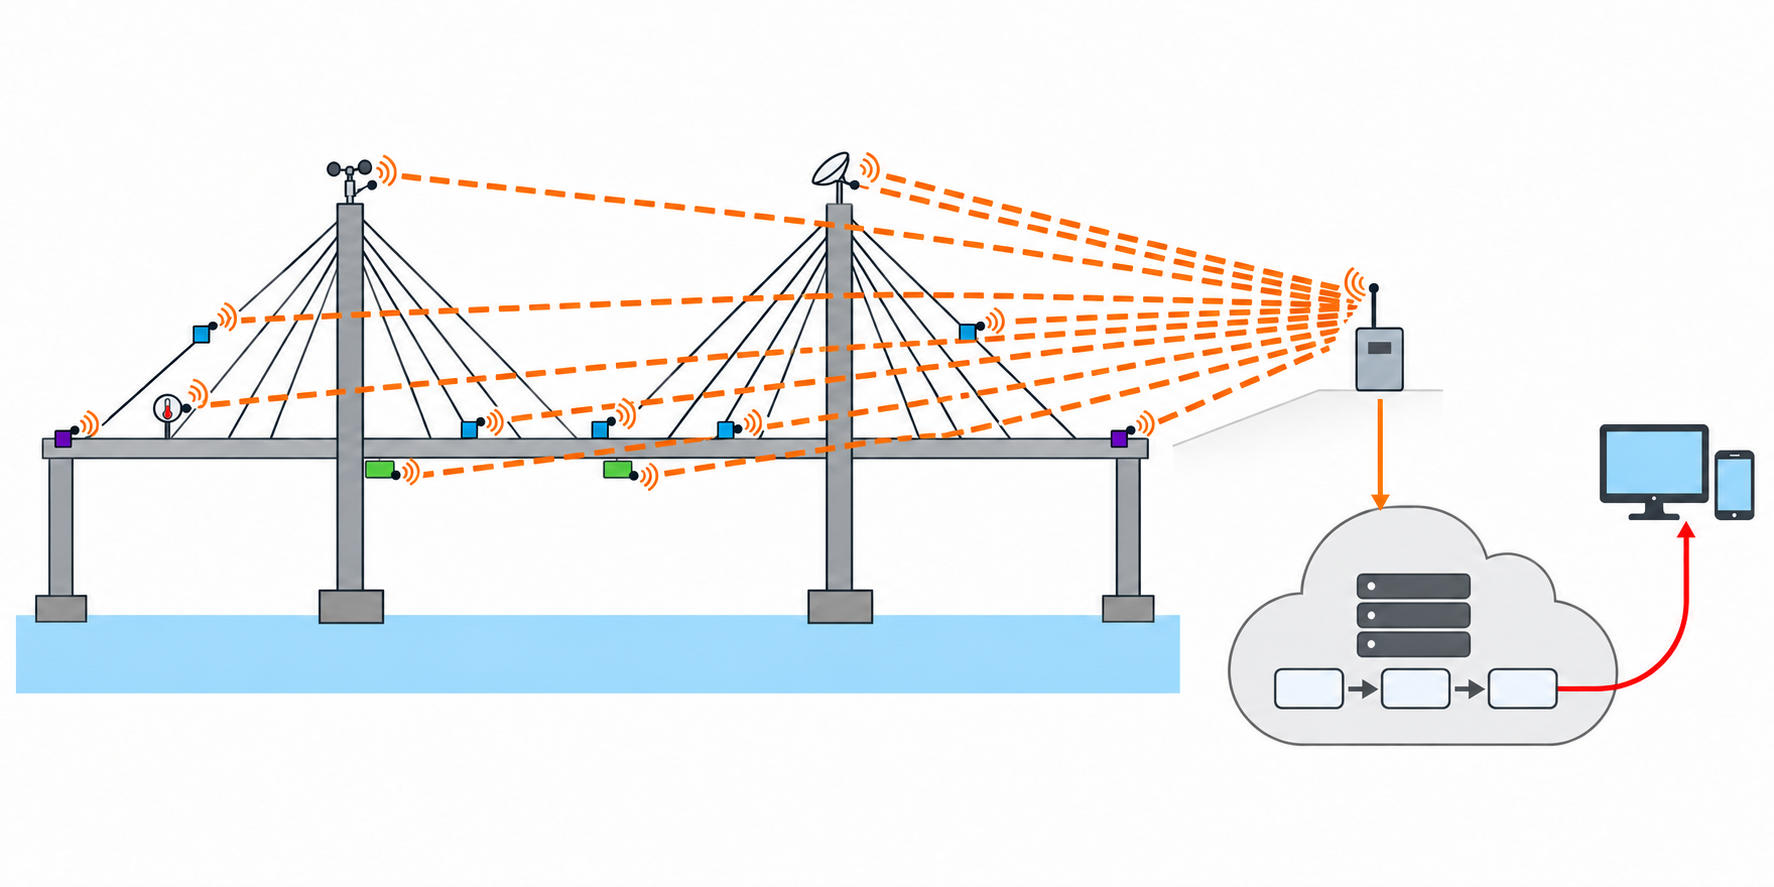
\includegraphics[width=\linewidth]{figures/ch11/ch11-06-v4-recovered.png}};
\begin{scope}[x={(img.south east)},y={(img.north west)}]
  \tikzset{
    lbl/.style={font=\sffamily\scriptsize,text=BookInk,fill=white,fill opacity=0.88,text opacity=1,inner sep=1.2pt,rounded corners=1pt,align=center},
    boxlbl/.style={font=\sffamily\tiny,text=BookInk,align=center,inner sep=0.5pt},
    ldr/.style={draw=BookInk!65,line width=0.45pt}
  }
  \node[lbl] (t1) at (0.11,0.77) {桥塔};
  \draw[ldr] (t1.east) -- (0.19,0.73);
  \node[lbl] (t2) at (0.33,0.76) {斜拉索（共 16 根）};
  \draw[ldr] (t2.south) -- (0.29,0.66);
  \node[lbl] (t3) at (0.56,0.42) {主梁};
  \draw[ldr] (t3.north) -- (0.56,0.49);
  \node[lbl,text=Ch11Orange!90!black] at (0.62,0.80) {无线传输链路};
  \node[lbl] (t5) at (0.86,0.64) {现场网关};
  \draw[ldr] (t5.west) -- (0.80,0.61);
  \node[lbl] at (0.80,0.45) {云端分析子系统};
  \node[boxlbl] at (0.738,0.224) {数据\\[-1pt]清洗};
  \node[boxlbl] at (0.798,0.224) {特征\\[-1pt]提取};
  \node[boxlbl] at (0.859,0.224) {阈值/\\[-1pt]异常判断};
  \node[lbl,text=Ch11Red,anchor=east] (t7) at (0.985,0.58) {预警通知管理人员\\[-1pt]{\tiny（需工程师复核）}};
  \draw[draw=Ch11Red,line width=0.45pt] (t7.south) -- (0.94,0.51);

  \draw[draw=BookRule,fill=BookPale!55,rounded corners=2pt,line width=0.4pt] (0.015,0.015) rectangle (0.985,0.115);
  \node[font=\sffamily\bfseries\tiny,text=BookInk,anchor=west] at (0.025,0.082) {传感器图例：};
  \filldraw[fill=Ch11Blue,draw=Ch11Gray,line width=0.4pt] (0.135,0.072) rectangle (0.147,0.092);
  \fill[black] (0.151,0.082) circle (0.0025);
  \node[font=\sffamily\tiny,text=BookInk,anchor=west] at (0.156,0.082) {加速度计（主梁 3 / 拉索 2）};
  \filldraw[fill=Ch11Green,draw=Ch11Gray,line width=0.4pt] (0.375,0.074) rectangle (0.393,0.090);
  \node[font=\sffamily\tiny,text=BookInk,anchor=west] at (0.398,0.082) {应变计（梁底 2）};
  \draw[Ch11Gray,line width=0.5pt] (0.535,0.070) -- (0.535,0.092);
  \draw[Ch11Gray,line width=0.5pt] (0.527,0.088) -- (0.543,0.088);
  \fill[Ch11Gray] (0.527,0.088) circle (0.003);
  \fill[Ch11Gray] (0.543,0.088) circle (0.003);
  \node[font=\sffamily\tiny,text=BookInk,anchor=west] at (0.548,0.082) {风速风向仪（左塔顶 1）};
  \draw[Ch11Gray,fill=white,line width=0.5pt] (0.715,0.084) ellipse (0.008 and 0.005);
  \draw[Ch11Gray,line width=0.5pt] (0.715,0.071) -- (0.715,0.080);
  \node[font=\sffamily\tiny,text=BookInk,anchor=west] at (0.727,0.082) {GNSS 天线（右塔顶 1）};
  \draw[Ch11Gray,fill=white,line width=0.5pt] (0.885,0.082) circle (0.006);
  \node[font=\sffamily\tiny,text=BookInk,anchor=west] at (0.894,0.082) {温度计（1）};

  \filldraw[fill=Ch11Purple,draw=Ch11Gray,line width=0.4pt] (0.028,0.030) rectangle (0.040,0.050);
  \node[font=\sffamily\tiny,text=BookInk,anchor=west] at (0.045,0.040) {位移计（两端 2）};
  \node[font=\sffamily\bfseries\tiny,text=BookInk,anchor=west] at (0.185,0.040) {连接线：};
  \draw[Ch11Gray,line width=0.6pt] (0.255,0.040) -- (0.285,0.040);
  \node[font=\sffamily\tiny,text=BookInk,anchor=west] at (0.290,0.040) {斜拉索（结构构件）};
  \draw[Ch11Orange,dashed,line width=1.1pt] (0.435,0.040) -- (0.470,0.040);
  \node[font=\sffamily\tiny,text=BookInk,anchor=west] at (0.475,0.040) {无线传输（传感器$\rightarrow$网关）};
  \draw[Ch11Orange,line width=1.1pt,-{Stealth[length=1.4mm]}] (0.665,0.040) -- (0.695,0.040);
  \node[font=\sffamily\tiny,text=BookInk,anchor=west] at (0.700,0.040) {广域网上传};
  \draw[Ch11Gray,line width=0.8pt,-{Stealth[length=1.3mm]}] (0.795,0.040) -- (0.820,0.040);
  \node[font=\sffamily\tiny,text=BookInk,anchor=west] at (0.825,0.040) {分析步骤};
  \draw[Ch11Red,line width=1.1pt,-{Stealth[length=1.4mm]}] (0.900,0.040) -- (0.930,0.040);
  \node[font=\sffamily\tiny,text=Ch11Red,anchor=west] at (0.935,0.040) {预警通知};
\end{scope}
\end{tikzpicture}
\caption{斜拉桥结构健康监测系统示意图（在 V4 底图上叠加 TikZ 标签与图例；教学用简化架构）。传感器布设于主梁、拉索与塔顶，数据经无线节点汇至现场网关，上传云端完成数据清洗、特征提取与阈值/异常判断，预警发送给管理人员并由工程师复核。图示不对应任何真实桥梁；实际系统常结合有线与无线传输，传感器数量与位置由具体设计决定。底图由图像模型生成，文字与图例以 TikZ 叠加；底图遗留偏差见表~\ref{tab:ch11-05}。}\label{fig:ch11-06}
\end{figure}

最后对照十项验收标准（F1--F10）完成整图复核（表~\ref{tab:ch11-05}）。如实列出底图尚未解决的局部偏差（拉索局部白隙、温度计内红色、云在网关下方、传感器图标偏小及待同行签字），才能明确正式投稿前在矢量软件里还需做哪几步收尾。

\begin{table}[htbp]\centering\footnotesize
\setlength{\tabcolsep}{3pt}
\renewcommand{\arraystretch}{1.15}
\caption{图~\ref{fig:ch11-06} 的十项整图核验记录。}\label{tab:ch11-05}
\begin{tabularx}{\linewidth}{@{}c>{\raggedright\arraybackslash}p{26mm}>{\raggedright\arraybackslash}p{16mm}Y>{\raggedright\arraybackslash}p{22mm}@{}}
\toprule
\textbf{\#} & \textbf{检查项} & \textbf{方法} & \textbf{实测结果与遗留偏差} & \textbf{结论} \\
\midrule
F1 & 双塔斜拉桥，无主缆/吊杆 & 目视 & 双塔斜拉桥侧视构型正确，无主缆或竖直吊杆 & 通过 \\
F2 & 拉索 16 根，均连塔与梁 & $200\%$ 计数 & 走向 $4+4+4+4=16$ 根，连塔与梁；但穿过图标与波纹处留有局部白隙 & 走向通过；断口待补线 \\
F3 & 12 个传感器类型与位置 & 对表计数 & $3+2+2+1+1+1+2=12$ 位置正确；温度计内部含红色，未精测同类色值 & 计数通过；温度计待去红 \\
F4 & L1--L4 方向与线型正确 & 逐条追踪 & 四类线语义方向正确，无越级直连；但云在网关下方使上传箭头朝下，局部有渐变 & 方向通过；上下布局有偏差 \\
F5 & 灰度下无线线与拉索可分 & 转灰度图 & 粗短虚线与细实线在灰度预览下可清楚区分 & 通过 \\
F6 & 底图无字，标签逐字比对 & $200\%$ 放大 & 底图零文字；TikZ 标签与图例逐字核对无误 & 通过 \\
F7 & $160\ \text{mm}$ 宽下图标 $\ge 2\ \text{mm}$、字 $\ge 6\ \text{pt}$ & 尺寸折算 & TikZ 文字 $\ge 6\ \text{pt}$；底图蓝方块折算约 $1.44\text{--}1.80\ \text{mm}$ 偏小 & 文字通过；小图标待放大 \\
F8 & 与 V2 相比无新意外变化 & 查修订表 & V4 相对 V2 未丢失或新增构件、传感器与箭头 & 通过 \\
F9 & 图注含简化与复核声明 & 读图注 & 已写明“教学用简化架构”与“预警由工程师复核” & 通过 \\
F10 & 结构工程同行复核签字 & 人工审阅 & 已完成作者核查；正式投稿前需结构工程同行复核签字 & 待同行签字 \\
\bottomrule
\end{tabularx}
\end{table}

\section{AI 在这一步能做什么与不能做什么}

修改与复核环节中 AI 与作者的分工汇总于表~\ref{tab:ch11-06}。

\begin{table}[htbp]\centering\footnotesize
\setlength{\tabcolsep}{3pt}
\renewcommand{\arraystretch}{1.15}
\caption{修改与复核环节中 AI 能做什么、不能做什么与作者要核对的内容。}\label{tab:ch11-06}
\begin{tabularx}{\linewidth}{@{}>{\raggedright\arraybackslash}p{18mm}YYY@{}}
\toprule
\textbf{环节} & \textbf{AI（\scidraw{} 等）能做} & \textbf{AI 不能做} & \textbf{作者要核对} \\
\midrule
理解意见 & 把一段口头意见改写成条目；按三层分类给出建议 & 判断哪条是科学错误（需领域知识与研究材料） & 每条问题能否定位到对象与位置；层级是否正确 \\
生成修改指令 & 把修改单条目改写成清楚的提示词 & 保证模型只执行这一条 & 指令包含“只改什么”和“保持不变”清单 \\
执行修改（图像） & 在 \scidraw{} 绘图中选历史图作参考并按指令多次迭代 & 对象锁定、区域保持；保证其他对象不变 & 每次修改后整图复核：对象计数、关系、文字、风格 \\
执行修改（数据图） & \scidraw{} 科学可视化可多轮对话修改，并恢复上一版或原版；由代码或配置重绘 & 判断修改后的统计表达是否仍正确 & 数据点、坐标轴、误差表达是否仍与数据一致 \\
比较版本 & （外部脚本）差异图、并排排版 & 产品内并排比较与命名（当前未提供，需下载后自行比较） & 人工按对象表计数；差异图只作辅助 \\
回退 & 重新选择历史中的某一版继续修改；数据图可一键恢复 & 自动判断哪一版是“正确基准” & 记录基准版本；在修订记录中写明“基于哪一版” \\
文字与精确样式 & — & 可靠拼写、精确色值与线型对齐 & 在排版层（TikZ/矢量软件）完成并逐字核对 \\
记录 & — & 自动生成可追溯的修订记录 & 每一版：基于、指令原文、目标修改、意外变化、复核结论、是否采用 \\
\bottomrule
\end{tabularx}
\end{table}

\section{本章检查清单}

\begin{itemize}
\item 每条意见都已翻译成“位置 + 现象”，并标注了层级（科学错误 / 阅读障碍 / 视觉一致性）。
\item 科学错误先于其他问题处理；科学错误多时选择重写输入而不是修补。
\item 修改单每条只说一件事，并写明“保持不变”的对象清单和核对方法。
\item 文字、精确色值、线型对齐类修改优先在排版层完成。
\item 每次生成式修改后，都按对象表与关系表**整图**复核，而不是只看改过的地方。
\item 与上一版并排比较；对象逐项计数；必要时用差异图辅助定位。
\item 发现连带变化后，回到上一个通过复核的版本，而不是在出错版本上叠加修改。
\item 同一修改两次仍有连带变化时，换路线（例如改在排版层完成）。
\item 修订记录中每一版都写明基于哪一版、指令原文、意外变化和是否采用；失败稿保留。
\item 终稿通过领域同行复核。
\end{itemize}

\section{练习}

\begin{enumerate}
\item \textbf{意见翻译（纸笔）。}拿出你最近收到的一条模糊意见（或用“这张图不够专业”），按本章三句追问，写出至少 6 条“位置 + 现象”问题，标注层级并排序，说明哪两条你会合并到同一次修改、哪一条要放到排版层处理。
\item \textbf{\scidraw{} 实操：连带变化实验。}在 \scidraw{} 绘图中生成或上传一张你自己的示意图作为 V2，选择它作为参考图，只要求改一处线型或颜色。生成后与 V2 并排，按你事先写好的对象表逐项计数，记录目标修改是否完成、有没有连带变化；然后回到 V2，加上保留清单重做一次，比较两次结果。把两次的记录整理成表~\ref{tab:ch11-04} 格式的修订记录。
\item \textbf{数据图对照。}在 \scidraw{} 科学可视化（\sdtool{sci-vis}）中上传一份公开数据或模拟数据，生成一张图后连续做三次修改（例如改配色、改坐标轴范围、改图例位置），再恢复到上一版和原版。写一段 200 字说明：数据图的修改和恢复与示意图的生成式修改有什么不同；为什么两者都仍需要整图复核。
\end{enumerate}

\section*{参考文献}

\begin{itemize}
\item Farrar CR, Worden K. An introduction to structural health monitoring. \textit{Philosophical Transactions of the Royal Society A}. 2007;365(1851):303--315. doi:10.1098/rsta.2006.1928
\item Kim S, Pakzad S, Culler D, Demmel J, Fenves G, Glaser S, Turon M. Health monitoring of civil infrastructures using wireless sensor networks. In: \textit{Proceedings of the 6th International Conference on Information Processing in Sensor Networks (IPSN '07)}. ACM; 2007:254--263. doi:10.1145/1236360.1236395
\item Ko JM, Ni YQ. Technology developments in structural health monitoring of large-scale bridges. \textit{Engineering Structures}. 2005;27(12):1715--1725. doi:10.1016/j.engstruct.2005.02.021
\item Lynch JP, Loh KJ. A summary review of wireless sensors and sensor networks for structural health monitoring. \textit{The Shock and Vibration Digest}. 2006;38(2):91--128. doi:10.1177/0583102406061499
\item Rougier NP, Droettboom M, Bourne PE. Ten simple rules for better figures. \textit{PLoS Computational Biology}. 2014;10(9):e1003833. doi:10.1371/journal.pcbi.1003833
\item Wong B. Simplify to clarify. \textit{Nature Methods}. 2011a;8(8):611. doi:10.1038/nmeth.1660
\item Wong B. Points of view: Color blindness. \textit{Nature Methods}. 2011b;8(6):441. doi:10.1038/nmeth.1618
\end{itemize}

% TODO: figures/ch11/ch11-03-v2-brief.png 与 figures/ch11/ch11-06-v4-recovered.png 尚存 4 处已知底图偏差（云在网关下方、温度计含红色、160 mm 宽下蓝方块约 1.44-1.80 mm 偏小、部分拉索穿过图标处有窄白隙），正文与表 11-3、11-4、11-5 已如实说明。
% TODO: figures/ch11/ch11-05-diff-and-count-zh.pdf 仅含第 7 章差异热图行与两案例计数表（表格末行底边略裁切）；若后续重跑脚本加入本章 V2/V3 差异热图行，需微调图 11-5 图注。
% TODO: figures/ch11/ch11-08-version-tree-zh.tex 图中节点 V3 文字为“连带变化（不采用）”，正文与图 11-8 图注已说明该分支用于示意出现连带变化时的回退逻辑。

\chapter{从论文配图到汇报与海报}

材料学博士生小周在第 9 章完成了钙钛矿太阳能电池界面改性论文的 Figure 2。那是一张双栏通栏的四面板组图：面板 a 交代平面器件的七层结构与钝化层位置，面板 b 给出截面层序的模型生成示意，面板 c 对比对照与改性器件的电流密度—电压（$J\text{--}V$）曲线，面板 d 展示连续光照 $1000\ \text{h}$ 内的归一化功率转换效率（PCE）衰减。整张图在 $174\ \text{mm}$ 印刷宽度下字号统一为 $8\ \text{pt}$，色彩与线型相互呼应，发给合作者审阅时获得了好评。

两周后，小周要在课题组大组会上作 10 分钟进展汇报；一个月后，他还要带一张 A0 竖版海报参加学术年会。为了省事，他把论文里的 Figure 2 整张截图拖进 16:9 幻灯片，在页面顶部打上“结果”两个大字（后文图~\ref{fig:ch12-05}a 将按后排视角还原这一页的效果）。到了组会现场，坐在会议室最后一排的同门眯着眼睛也看不清横纵坐标的数字；小周刚讲完面板 a 的器件层序准备切入效率对比，导师却打断他问：“右边那张图里哪条线是对照？面板 b 那张电镜图是你自己拍的吗？”原来，论文图注没有跟着截图进幻灯片，而面板内的标注在缩放与重采样后变得模糊不清。

组会结束后，小周又开始排会议海报。他把论文的摘要、引言、方法和结论按三栏原样贴满画布，再把那张四面板组图等比放大塞进海报正中央。把草稿缩略图发给师姐看时，师姐只问了一句：“如果有人从展板通道走过去，五秒钟内能看出你到底改了哪一层、效率提高了多少吗？”

小周手里的科学证据没有任何变化，为什么在论文里合格的组图，到了报告厅和海报展区却接连失效？原因在于论文、口头汇报和学术海报面对的是三种截然不同的观看条件。本章围绕同一项钙钛矿界面改性研究（采用标准单二极管模型生成的模拟教学数据），系统讲解如何用视角换算确定字号与线宽，如何把四面板论文组图拆解为逐步揭示的 16:9 汇报页，如何按三层阅读距离规划 A0 竖版海报，以及如何在 \scidraw{} 中完成重绘、模板排版与跨版本一致性核验。

\section{同一研究，三种观看条件}

很多研究者在准备学术报告或会议海报时，习惯把它们当成“论文的缩减版”——从论文文档里挑几张图、复制几段话，塞进不同尺寸的画布里。这种做法忽略了一个基本事实：读者在书桌前读论文、听众在报告厅看投影屏幕、参会者在展厅通道里浏览海报，这三种场景在\textbf{观看距离、可用时间、节奏由谁控制}三个物理与认知变量上存在数量级的差异（图~\ref{fig:ch12-01}）。

\begin{figure}[htbp]\centering
\resizebox{\linewidth}{!}{% FIG ch12-01 three viewing conditions (Chinese)
\begin{tikzpicture}[
  x=1mm, y=1mm,
  font=\sffamily\small,
  text=BookInk,
  coltitle/.style={font=\sffamily\bfseries, text=BookTeal, align=center},
  cell/.style={draw=BookRule, fill=white, align=left, text width=42mm, inner sep=2mm, minimum height=9mm},
  emphcell/.style={cell, fill=BookPale, draw=BookTeal, font=\sffamily\bfseries\small},
  icon/.style={draw=BookInk!40, fill=BookPale, line width=0.5pt},
]
  % Column headers with scale icons (1 m bar shared)
  \def\colX{22, 72, 122}
  \foreach \x/\name/\w/\h in {22/论文/42/59, 72/汇报/64/36, 122/海报/42/59} {
    \begin{scope}[shift={(\x, 108)}]
      \node[coltitle] at (21, 14) {\name};
      \draw[icon, fill=white] (6, 0) rectangle ++(\w, \h);
      \ifnum\x=72
        \draw[BookInk!60, line width=0.8pt] (10, 4) -- (54, 4);
        \draw[BookInk!60, line width=0.8pt] (10, 32) -- (54, 32);
      \fi
    \end{scope}
  }
  \draw[BookTeal, line width=1pt] (10, 100) -- ++(20, 0);
  \node[font=\scriptsize, anchor=west] at (32, 100) {1 m（比例尺）};

  \node[cell, anchor=north west] at (0, 98) {观看距离};
  \node[cell] at (22, 89) {30--50 cm};
  \node[cell] at (72, 89) {2--15 m};
  \node[cell] at (122, 89) {先 2--5 m\\再 0.5--1.5 m};

  \node[cell, anchor=north west] at (0, 78) {可用时间};
  \node[cell] at (22, 69) {读者自定};
  \node[cell] at (72, 69) {每页约 1--2 分钟};
  \node[cell] at (122, 69) {几秒决定是否停留\\停留后数分钟};

  \node[cell, anchor=north west] at (0, 58) {节奏控制};
  \node[cell] at (22, 49) {读者};
  \node[cell] at (72, 49) {讲者};
  \node[cell] at (122, 49) {观众};

  \node[cell, anchor=north west] at (0, 38) {谁来解释};
  \node[cell] at (22, 29) {图注};
  \node[cell] at (72, 29) {讲者};
  \node[cell] at (122, 29) {海报自身};

  \node[emphcell, anchor=north west] at (0, 18) {内容策略};
  \node[emphcell, text=BookTeal] at (22, 9) {密而自足};
  \node[emphcell, text=BookTeal] at (72, 9) {少而顺序化};
  \node[emphcell, text=BookTeal] at (122, 9) {分层};
\end{tikzpicture}
}
\caption{三种观看条件。距离和时间为常见工作条件，具体以会场与学校要求为准。}\label{fig:ch12-01}
\end{figure}

先看图~\ref{fig:ch12-01} 顶部的尺度示意。若把一页 A4 论文（宽 $210\ \text{mm}$、高 $297\ \text{mm}$）、一块常见报告厅的 16:9 投影屏幕（如宽约 $3.6\ \text{m}$、高约 $2.0\ \text{m}$）和一张 A0 竖版海报（宽 $841\ \text{mm}$、高 $1189\ \text{mm}$）放在同一比例尺下对比，画幅面积相差十余倍乃至上百倍。但画幅变大并不意味着能够装进更多细节，因为观众与画面的距离拉得更远。

\textbf{第一个变量是观看距离。}阅读打印出来的论文或笔记本电脑屏幕时，人眼到画面的距离通常稳定在 $30\text{--}50\ \text{cm}$。遇到密集的坐标刻度或细小的面板标注，读者随时可以把页面凑近到 $25\ \text{cm}$，或者在电子版 PDF 中放大到 $200\%$ 查看。口头汇报则完全不同：中小型会议室或组会教室里，听众距离屏幕约 $2\text{--}10\ \text{m}$；大型学术会议分会场里，后排听众距离屏幕可达 $12\text{--}15\ \text{m}$。听众被固定在座位上，不可能走到讲台前贴着幕布看坐标轴。学术海报的观看距离则是分阶段的：参会者沿着展厅通道边走边看时，距离海报板约 $2\text{--}5\ \text{m}$；只有当海报顶部的标题或核心图形吸引了他的注意，他才会停下脚步，走到 $1\text{--}2\ \text{m}$ 处浏览主要结论区块，最后在感兴趣的局部凑近到 $0.5\text{--}1.5\ \text{m}$ 细看实验参数或方法说明。

\textbf{第二个变量是可用时间。}论文阅读的时长完全由读者自己决定。审稿人或小同行可以对一张包含四个面板、几十个数据点的组图反复推敲十分钟，对照正文和图注逐行核查。口头汇报中，每一页幻灯片在屏幕上停留的时间通常只有 $1\text{--}2\ \text{分钟}$（10 分钟的短报告往往只有 8 至 10 页正文页）。在这短短几十秒里，听众不仅要看画面，还要同时听讲者的口头解释；一旦画面上同时出现四张子图和大段文字，视觉搜索就会与听觉理解争夺有限的工作记忆。海报展区的时间分配更加苛刻：路过者在通道里扫视一张海报往往只花几秒钟，在这几秒钟内决定“继续往前走”还是“停下来看”；即便停下来，大多数观众在一张海报前停留的时间也只有几分钟。

\textbf{第三个变量是节奏控制者与解释责任。}在论文里，阅读节奏由读者掌控：读者可以先看面板 a 再看面板 c，也可以随时低头读图注；因此论文配图依靠\textbf{图注与正文}共同完成解释。在口头汇报里，翻页和揭示的节奏掌握在\textbf{讲者}手中：听众无法倒退回上一页，也看不到论文里那段两百字的图注；讲者站在屏幕旁，用口头讲述、手势和分步动画承担了背景交代与逻辑串联工作（Bourne，2007；Naegle，2021）。而在海报展区，节奏重新回到\textbf{观众}手里，但情况比论文更特殊——在两三个小时的海报展示时段内，作者可能正在向另一位同行解释问题，也可能暂时离开展位去听其他报告。这意味着一张合格的学术海报必须能够\textbf{自我解释}：即使作者不在场，驻足的同行也能顺着版面指引看懂研究问题、主要结果和基本条件（Erren 与 Bourne，2007）。

把这三个变量合在一起，就能直接推导出同一项研究在三种媒介中的内容密度策略（图~\ref{fig:ch12-01} 底部）：
\begin{itemize}
\item \textbf{论文配图——密而自足：}因为观看距离近、阅读时间充裕且有完整图注配合，可以把结构示意、形貌对照、核心性能与稳定性证据紧凑地组织在同一张双栏组图中，让读者在一处完成跨面板比对。
\item \textbf{口头汇报——少而顺序化：}因为距离远、每页停留时间短且有讲者现场引导，必须把多面板组图拆开，按照“提出改动 $\rightarrow$ 展示效率提升 $\rightarrow$ 展示稳定性改善”的时间顺序分页呈现；每页只保留一个核心结论句和一组支撑证据，其余背景由讲者口头补足。
\item \textbf{学术海报——分层：}因为观众经历了“远距离扫视 $\rightarrow$ 中距离读结论 $\rightarrow$ 近距离查细节”的空间移动，版面必须按阅读距离分层设计：在 $2\text{--}5\ \text{m}$ 外就能看清研究问题与一句话主结论，在 $1\text{--}2\ \text{m}$ 处能读完三个核心证据区块，在 $0.5\ \text{m}$ 处能查到关键方法参数与证据声明。
\end{itemize}

需要说明的是，图~\ref{fig:ch12-01} 中列出的距离与时间是科研交流中的常见工作条件，而非硬性标准。不同学校学位答辩的投影设备、不同学术会议的报告厅景深与海报展板规格各有差异，动手排版前应先查阅会议官方网站或向组织者确认场地尺寸与时间要求。

\section{用视角估算字号}

明确了三种观看条件之后，紧接着会遇到一个最常见的具体问题：“我的幻灯片和海报字号到底该设多大？”许多经验帖会给出一张死板的字号表，比如“PPT 正文一律 24 pt，海报正文一律 28 pt”。然而，在小会议室里 5 米外看 85 英寸电视屏幕，与在阶梯报告厅里 14 米外看一块偏小的投影幕布，所需的幻灯片字号显然不可能相同。与其死记硬背数字，不如用基本的几何光学原理，把字号选择变成一道两步就能算完的简单算术题。

人眼能否轻松辨认一个字符，不取决于字符在纸面或屏幕上的绝对毫米高度 $h$，而取决于它在视网膜上所张开的\textbf{视角（visual angle）} $\theta$。当观看距离 $d$ 远大于字符高度 $h$ 时，由小角近似公式可得：
\[
\theta \approx \frac{h}{d}
\]
其中 $\theta$ 以弧度为单位；在本章涉及的字号与距离范围内，小角近似误差小于 $0.1\%$。也就是说，要让远处观众看字的轻松程度与近处读论文相当，字符的物理高度 $h$ 必须与观看距离 $d$ 成正比放大。在印刷与排版中，字号通常以点（point，简写为 $\text{pt}$）为单位，$1\ \text{pt} = 1/72\ \text{in} \approx 0.3528\ \text{mm}$（指字身框标称高度，汉字字面高度与拉丁字母大写高度、$x$ 高度均随字号成正比缩放）。只要选定一个日常阅读论文时的舒适基准，就能换算出任意距离下的等效字号（图~\ref{fig:ch12-02}）。

\begin{figure}[htbp]\centering
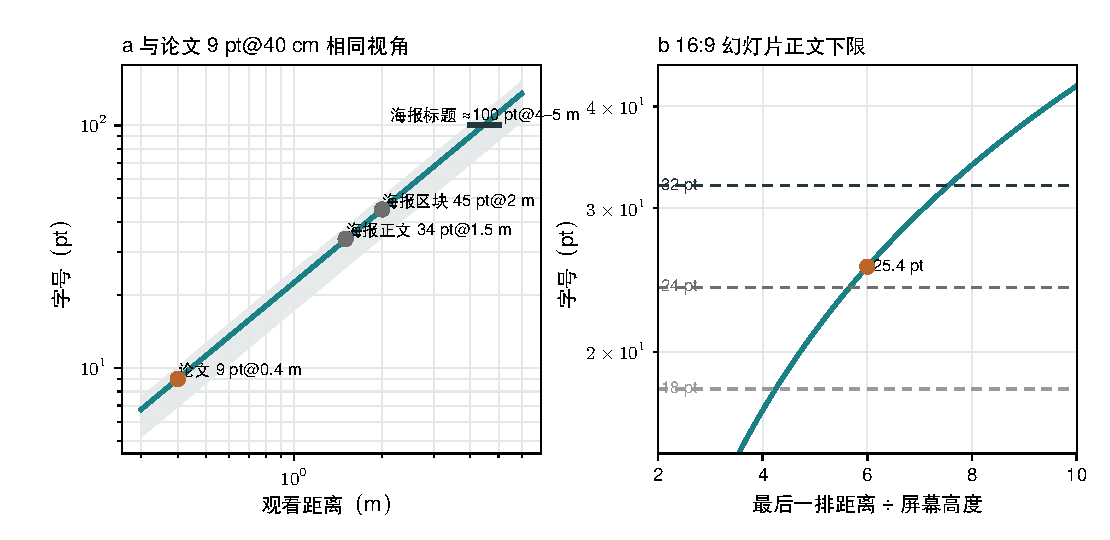
\includegraphics[width=\linewidth]{figures/ch12/ch12-02-visual-angle-text-size-zh.pdf}
\caption{由视角换算的字号。曲线给出与在 40 cm 处阅读 9 pt 文字相同的视角所需字号；这是几何推算，不是期刊或会议规定。投影较暗、观众视力或语言条件不利时应进一步放大。}\label{fig:ch12-02}
\end{figure}

下面我们分论文、海报和口头汇报三个场景，逐步推算图~\ref{fig:ch12-02} 中的曲线与关键工作点。

\textbf{第一，建立论文阅读基准。}在阅读纸质期刊或平板电脑时，常见阅读距离约为 $d_0 = 40\ \text{cm} = 400\ \text{mm}$。期刊正文与清晰图表标注常用的字号约为 $s_0 = 9\ \text{pt}$（标称字高 $h_0 = 9 \times 0.3528 \approx 3.18\ \text{mm}$；期刊配图允许的最小刻度字号通常在 $7\text{--}8\ \text{pt}$ 左右）。以“在 $40\ \text{cm}$ 处阅读 $9\ \text{pt}$ 文字”作为本书的参照基准，其对应的张角为：
\[
\theta_0 \approx \frac{3.18\ \text{mm}}{400\ \text{mm}} \approx 0.00794\ \text{rad} \approx 0.45^\circ
\]
如果把论文配图中常见的 $7\text{--}10\ \text{pt}$ 范围一并换算，在 $40\ \text{cm}$ 处对应的视角范围约为 $0.35^\circ\text{--}0.50^\circ$（即图~\ref{fig:ch12-02}a 中的浅灰色阴影带）。这里要特别说明：“$40\ \text{cm}$ 处的 $9\ \text{pt}$”是我们为了方便心算而选定的几何参照点，并不是哪家期刊或国际标准组织的强制规定。

\textbf{第二，按实际打印尺寸换算海报字号（图~\ref{fig:ch12-02}a）。}学术海报通常按 1:1 的物理尺寸排版并打印。因此，要让站在距离海报 $d$（单位：$\text{m}$）处的观众获得与“$0.4\ \text{m}$ 处读 $9\ \text{pt}$”完全相同的视角，所需的海报字号 $s_{\text{poster}}$ 只需按距离倍数线性放大：
\[
s_{\text{poster}}(d) = 9 \times \frac{d}{0.4\ \text{m}}\ \text{pt} = 22.5\,d\ \text{pt}
\]
将上一节海报展区的三个典型阅读距离代入上式，立刻可以得到三层信息的基准字号：
\begin{itemize}
\item \textbf{细节层与近距阅读（$d = 1.0\text{--}1.5\ \text{m}$）：}当观众停步走近到 $1.0\ \text{m}$ 时，等效字号为 $9 \times 1.0 / 0.4 = 22.5\ \text{pt}$；若观众站在 $1.5\ \text{m}$ 处（常见于两人并排站在展板前阅读或讨论），等效字号为 $9 \times 1.5 / 0.4 = 33.75\ \text{pt} \approx 34\ \text{pt}$（图~\ref{fig:ch12-02}a 中间的深灰圆点）。因此，海报上需要在 $1.5\ \text{m}$ 处轻松看清的正文要点与数据图坐标轴，字号设在 $28\text{--}34\ \text{pt}$ 才有几何保障；即便是供 $0.5\text{--}1.0\ \text{m}$ 近看的方法细则或参考文献，也不宜低于 $24\ \text{pt}$。
\item \textbf{结论层标题（$d = 2.0\ \text{m}$）：}为了让站在两米外或斜侧方的观众一眼捕捉到每个证据区块的结论句，代入 $d = 2.0\ \text{m}$ 可得 $9 \times 2.0 / 0.4 = 45\ \text{pt}$。
\item \textbf{顶部主标题带（$d = 4.0\text{--}5.0\ \text{m}$）：}为了让通道上的路过者在四五米外看清研究问题，代入 $d = 4.5\ \text{m}$ 可得 $9 \times 4.5 / 0.4 \approx 101\ \text{pt}$（对应 $4\text{--}5\ \text{m}$ 区间的 $90\text{--}113\ \text{pt}$，图~\ref{fig:ch12-02}a 右上方的深色横线段）。
\end{itemize}

\textbf{第三，用“距离与屏幕高度之比”换算汇报幻灯片字号（图~\ref{fig:ch12-02}b）。}幻灯片与海报有一点本质不同：你排好一页 16:9 幻灯片后，它最终在会场里有多大，取决于报告厅投影屏幕的物理高度 $H$。在 PowerPoint 或 Keynote 的标准 16:9 宽屏设置中，画布尺寸为 $13.333 \times 7.5\ \text{in}$（即 $33.867 \times 19.05\ \text{cm}$），画布总高度固定对应 $7.5 \times 72 = 540\ \text{pt}$。当你在幻灯片上使用字号 $s_{\text{slide}}$（单位：$\text{pt}$）时，单个字符占整个屏幕高度的比例就是 $s_{\text{slide}} / 540$。设会场屏幕的物理高度为 $H$，最后一排听众到屏幕的距离为 $D$，则字符在最后一排听众眼中的张角为：
\[
\theta \approx \frac{(s_{\text{slide}} / 540)\,H}{D} = \frac{s_{\text{slide}}}{540 \times (D/H)}
\]
反过来，若要求最后一排听众看到的视角达到 $\theta_0 \approx 0.45^\circ \approx 0.00785\ \text{rad}$，则幻灯片字号只需由无量纲比值 $D/H$（最后一排距离除以屏幕高度）决定：
\[
s_{\text{slide}} \approx 0.00785 \times \left(\frac{D}{H}\right) \times 540\ \text{pt} \approx 4.24 \times \left(\frac{D}{H}\right)\ \text{pt}
\]
我们看两个具体算例。算例一：某标准学术报告厅的投影屏幕高 $H = 2.0\ \text{m}$（16:9 屏幕宽约 $3.56\ \text{m}$），最后一排距屏幕 $D = 12\ \text{m}$，此时距离与屏高之比 $D/H = 6$。如果在幻灯片上使用 $24\ \text{pt}$ 文字，字符占屏高的 $24 / 540 = 1 / 22.5$，投影到幕布上高约 $8.9\ \text{cm}$，在 $12\ \text{m}$ 处的张角约为 $0.42^\circ$；若按 $0.45^\circ$ 严格计算，所需字号约为 $25.4\ \text{pt}$（图~\ref{fig:ch12-02}b 中的橙褐色圆点）。这就从几何上解释了一条非常实用的经验法则：\textbf{当会场最后一排距离不超过屏幕高度的 6 倍（$D/H \le 6$）时，24 pt 是幻灯片正文与轴标题较为稳妥的下限，坐标刻度也不宜小于 20 pt。}

算例二：如果换到一间狭长的教室，屏幕高只有 $H = 1.5\ \text{m}$，而后排距离达到 $D = 8\ \text{m}$（$D/H \approx 5.33$），此时若在图中使用 $18\ \text{pt}$ 的小字（占屏高 $1/30$），在 $8\ \text{m}$ 处的张角只有 $(1.5 / 30) / 8 \approx 0.00625\ \text{rad} \approx 0.36^\circ$，已经退化到接近论文最小字号的下限（顺便留意，图~\ref{fig:ch12-02}b 左缘的参考线文字 \texttt{18 pt}、\texttt{24 pt}、\texttt{32 pt} 紧贴左轴框内侧并压在了水平虚线上，自己在制作参考线标注时，最好把文字放在虚线上方或右端空白处以避开线条）。

\textbf{第四，同步换算线宽与数据标记。}视角原理同样适用于曲线粗细、坐标轴边框、刻度线和散点符号。在 $40\ \text{cm}$ 处阅读论文时，$0.5\text{--}0.8\ \text{pt}$ 的坐标轴线与 $1.2\ \text{pt}$ 的数据曲线清晰利落；但如果把 $0.5\ \text{pt}$ 细线原封不动放到 $1.5\ \text{m}$ 外观看的海报上，需按距离放大 $1.5 / 0.4 = 3.75$ 倍才能保持同等视觉粗细。因此，幻灯片与海报上的数据曲线和轴线应加粗到 $2.0\text{--}3.5\ \text{pt}$。此外，遇到投影仪发暗、环境光过强、听众坐在大角度侧排或阅读非母语术语时，都应在几何推算值的基础上进一步放大。

\section{从论文组图拆出一组汇报页}

现在回到小周的钙钛矿太阳能电池案例。我们先把第 9 章定稿的论文版 Figure 2（图~\ref{fig:ch12-03}）摆在面前，看看它为什么适合论文，却不适合直接放进幻灯片。

\begin{figure}[htbp]\centering
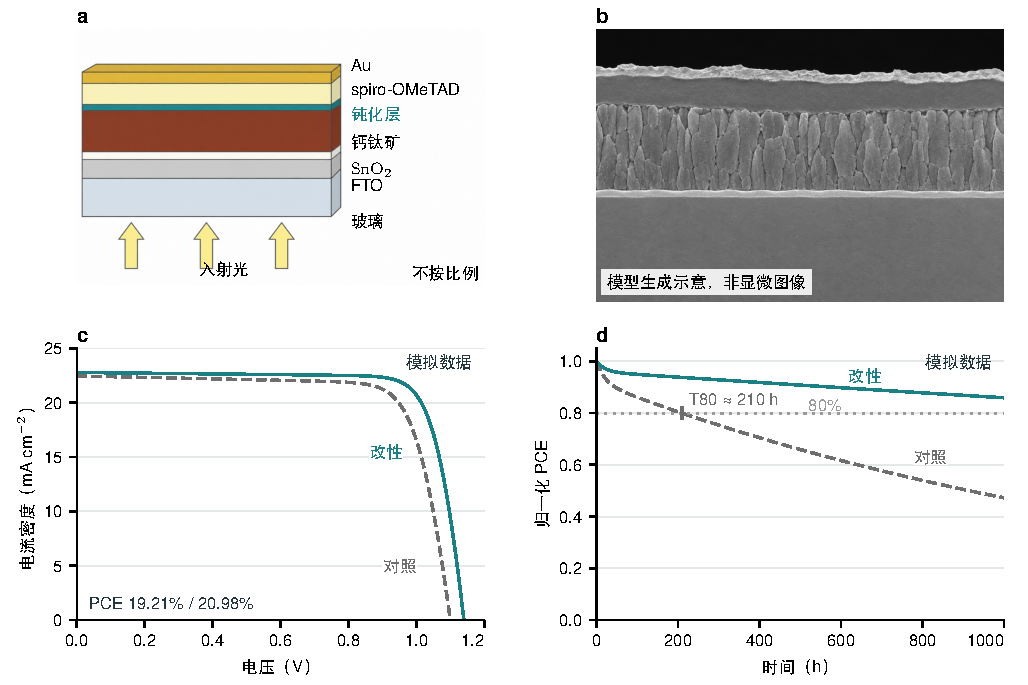
\includegraphics[width=\linewidth]{figures/ch12/ch12-03-paper-figure-2-zh.pdf}
\caption{论文版 Figure 2（第 9 章）。c、d 为模拟数据；b 为模型生成示意，非显微图像；a 不按比例。}\label{fig:ch12-03}
\end{figure}

在图~\ref{fig:ch12-03} 中，四个面板按 $2 \times 2$ 网格紧凑排列在 $174 \times 116\ \text{mm}$ 的双栏画布上：上排左侧面板 a 用七层色块交代玻璃、FTO、$\text{SnO}_2$、钙钛矿、青色钝化层、spiro-OMeTAD 与 Au 背电极的叠层顺序，并在右下角注明“不按比例”；上排右侧面板 b 放置灰度类 SEM 截面图样，左下角用浅白底框明确标注“模型生成示意，非显微图像”；下排面板 c 与 d 分别绘制模拟 $J\text{--}V$ 曲线与 $1000\ \text{h}$ 归一化 PCE 稳定性曲线，统一使用灰色虚线代表对照、青色实线代表改性，并在右上角标明“模拟数据”。然而，当小周把图~\ref{fig:ch12-03} 整张贴进 16:9 幻灯片，并在会场最后一排观看时，效果就变成了图~\ref{fig:ch12-05}a。

\begin{figure}[htbp]\centering
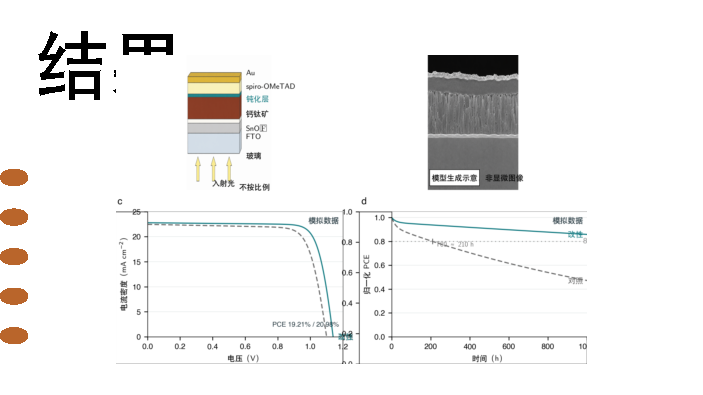
\includegraphics[width=119mm]{figures/ch12/ch12-05a-pasted-zh.pdf}\\[1mm]
{\footnotesize (a) 直接贴入论文组图：左侧橙褐色圆点 (1)--(5) 对应正文分析的五项问题}\\[3mm]
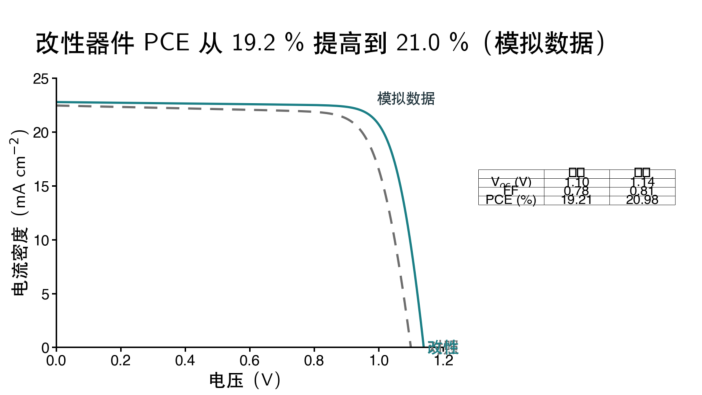
\includegraphics[width=119mm]{figures/ch12/ch12-05b-rebuilt-zh.pdf}\\[1mm]
{\footnotesize (b) 按汇报条件重绘的第 2b 页：单一问题、结论标题与大字号直接标注}
\caption{同一页内容从会场最后一排看到的大小。两图按 119 mm 宽印刷：在 40 cm 处阅读它们，与在 12 m 外看 3.6 m 宽的屏幕视角相同。（a）直接贴入论文组图；（b）按汇报重绘。数据为模拟数据。}\label{fig:ch12-05}\label{fig:ch12-05a}\label{fig:ch12-05b}
\end{figure}

图~\ref{fig:ch12-05} 的印刷宽度经过了精确的视角匹配：在 $12\ \text{m}$ 外看宽 $3.56\ \text{m}$ 的 16:9 投影屏幕，横向视角与在 $40\ \text{cm}$ 处看宽 $119\ \text{mm}$ 的书页完全相同（$3.56 / 12 \times 400\ \text{mm} \approx 119\ \text{mm}$）。因此，两图在书中固定按 $119\ \text{mm}$ 宽印刷，读者在正常阅读距离看到的正是后排听众眼中的真实画面。沿着图~\ref{fig:ch12-05}a 左侧页边的五个橙褐色编号圆点 (1)--(5)，可以清楚看到“整张贴图”暴露出的五项问题：
\begin{enumerate}
\item \textbf{刻度与轴标题过小（对应圆点 1）：}把 $174\ \text{mm}$ 宽、$8\ \text{pt}$ 字（或 $180\ \text{mm}$ 宽、$7\ \text{pt}$ 字）的组图缩放到占 16:9 页面宽度 $90\%$（约 $305\ \text{mm}$）时，在幻灯片坐标系中的等效字号只有约 $12\text{--}14\ \text{pt}$。放到 $12\ \text{m}$ 处观看，视角仅约 $0.21^\circ\text{--}0.25^\circ$，不到论文阅读视角的一半，后排听众根本看不清横轴电压和纵轴电流密度。
\item \textbf{标注挤压、边框重叠与识别困难（对应圆点 2）：}若原论文图使用角落里的独立图例框，听众需要在图例和曲线间来回对照；而即便原图使用了直接标注，在贴图重采样与窄高画布压缩下，图~\ref{fig:ch12-05}a 下排面板 c 的右框线与面板 d 的左轴刻度（\texttt{1.0}、\texttt{0.8}、\texttt{0.6}）直接叠在一起，面板 c 右下角的“对照/改性”与刻度 \texttt{1.2} 撞成一团，面板 d 中的 \texttt{T80} 标注也压在了灰色虚线上。
\item \textbf{四个面板同时争夺注意力（对应圆点 3）：}四个面板同时亮在屏幕上，讲者讲面板 c 时听众却在看面板 a 或 b；且粗暴贴图造成了边缘裁切——上排面板字母 \texttt{a}、\texttt{b} 被裁掉，面板 d 横轴最右侧的 \texttt{1000} 被截成了 \texttt{10}。
\item \textbf{页标题没有结论（对应圆点 4）：}页面左上角只写了“结果”二字（且在图~\ref{fig:ch12-05}a 中因文本框裁切只露出左半边），没有传递任何科学发现。
\item \textbf{证据状态声明受损或丢失（对应圆点 5，诚信高风险项）：}原本写在论文图注里的模拟条件随截图一起丢失；面板 b 左下角的“模型生成示意，非显微图像”在贴图重绘时，“非显微图像”五个黑字溢出了白色底框、落在了深灰色背景上，在后排视角下几乎无法辨认（面板 a 中 $\text{SnO}_2$ 的下标也因字体缺字变成了方框），极易让听众把模型生成的示意形貌误认为真实电镜照片。
\end{enumerate}

要把图~\ref{fig:ch12-03} 改造成像图~\ref{fig:ch12-05}b 那样在后排依然清晰的汇报页，应按以下六个步骤，将空间并列的论文组图重构为时间顺序化的 16:9 幻灯片序列（图~\ref{fig:ch12-04}）：

\begin{figure}[htbp]\centering
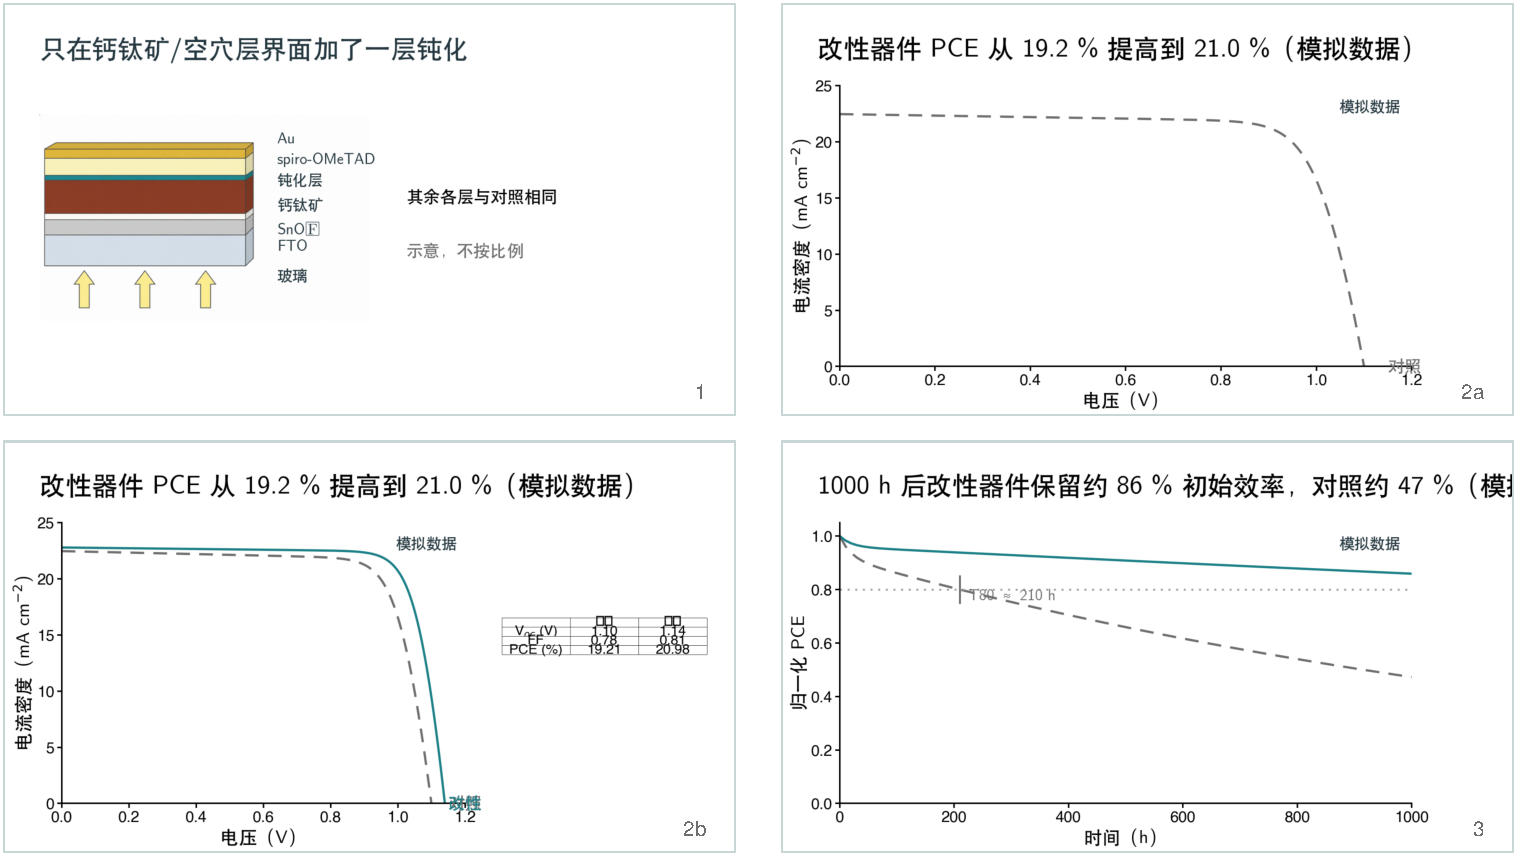
\includegraphics[width=\linewidth]{figures/ch12/ch12-04-slide-sequence-zh.pdf}
\caption{由同一组数据拆出的三页汇报（第 2 页分两步）。每页标题是结论句，图中直接标注曲线；数值、坐标范围与颜色语义与论文版一致。数据为模拟数据。}\label{fig:ch12-04}
\end{figure}

\textbf{第一步，列出组图回答的子问题，把次要面板移入备用页。}论文 Figure 2 依次回答三个核心问题：(1) 器件结构做了什么改动？(2) 初始效率提高了多少？(3) 运行 $1000\ \text{h}$ 后的稳定性改善了多少？面板 b 的类 SEM 截面示意不承担主结论的定量证明，因此不放进 3 分钟的正文汇报页，而是连同完整的“模型生成示意，非显微图像”标注移入报告末尾的备用页，留待问答环节调用。

\textbf{第二步，每页只回答一个子问题，把页标题写成完整结论句。}采用常见的“断言—证据（assertion--evidence）”写法（Naegle，2021），在每页顶部用 $32\text{--}36\ \text{pt}$ 直接写出本页结论并保留证据性质标注：第 1 页写“只在钙钛矿/空穴层界面加了一层钝化”，第 2 页写“改性器件 PCE 从 $19.2\%$ 提高到 $21.0\%$（模拟数据）”，第 3 页写“$1000\ \text{h}$ 后改性器件保留约 $86\%$ 初始效率，对照约 $47\%$（模拟数据）”。

\textbf{第三步，设计分步揭示（progressive reveal）。}将第 2 页拆为完全对齐的两帧（第 2a 页与第 2b 页）：先切出第 2a 页，画面上只有坐标轴与灰色虚线“对照”曲线，讲者口头带听众读懂横纵坐标含义；随后翻到第 2b 页（即图~\ref{fig:ch12-05}b），在横纵坐标范围分毫不差的同一坐标系上，叠加青色实线“改性”曲线并在右侧亮出 $V_{\text{oc}}$、$\text{FF}$ 与 $\text{PCE}$ 简表。两帧坐标范围完全一致，翻页时曲线不跳动，听众能立即看清改性带来的增量。

\textbf{第四步，删去面板字母与长图例，改为直接标注。}删去 \texttt{a}--\texttt{d} 面板字母和独立图例框，在曲线旁直接标“对照”“改性”，并在第 1 页器件结构图上用橙褐色粗框高亮新增的钝化层，右侧只留两行要点（“其余各层与对照相同”“示意，不按比例”）。

\textbf{第五步，按 16:9 原生尺寸重绘，并放大检查排版细节。}每页按 $13.333 \times 7.5\ \text{in}$ 原生画布绘制（页标题 $34\ \text{pt}$，轴标题 $24\ \text{pt}$，刻度 $20\ \text{pt}$，标注 $22\ \text{pt}$，线宽 $3\ \text{pt}$），绝不拉伸原图。同时，对照图~\ref{fig:ch12-04} 的实际出图画面做原尺寸复查，能抓出四处需要在上台前修正的细节：(1) 第 1 页层名中的 $\text{SnO}_2$ 若直接使用 Unicode 下标字符，在中文字体下会因缺字变成方框，应改为数学模式 \texttt{\$\textbackslash mathrm\{SnO\_2\}\$} 或在演示软件中用文本框下标；(2) 第 2a、2b 页若把直接标注简单绑在曲线最末一个点（$J = 0$）右侧，“对照”与“改性”会叠在横轴右端并与刻度 \texttt{1.2} 碰撞（图~\ref{fig:ch12-05}b 右下角同样可见），应将标签上移到曲线陡降段的中部空白处；(3) 第 2b 页右侧用绘图函数生成小表时，表头单元格因未显式绑定中文字体出现了两个方框且行高偏紧，实际制作幻灯片时直接在 PowerPoint 中插入原生表格更稳妥；(4) 第 3 页标题字数较多，单行 $34\ \text{pt}$ 在画布右缘被截掉半个括号，应手动换行或微调至 $30\ \text{pt}$。

\textbf{第六步，保持数值、坐标范围、颜色语义与证据声明一致。}全部数值、轴范围（$0\text{--}1.2\ \text{V}$，$0\text{--}25\ \text{mA cm}^{-2}$，$0\text{--}1000\ \text{h}$；若改变范围须在讲稿中说明）、灰虚线对照与青实线改性、以及图内右上角的“模拟数据”标注，均与论文版保持严格一致。

\section{A0 竖版海报：栅格、层次与密度}

按照国际标准 ISO 216，\textbf{A0 竖版海报}的物理尺寸为 $841 \times 1189\ \text{mm}$，面积恰好为 $1\ \text{m}^2$。规划海报版面之前，先看展厅里的真实观看过程（图~\ref{fig:ch12-07}）。

\begin{figure}[htbp]\centering
\begin{tikzpicture}
\node[anchor=south west,inner sep=0] (img) at (0,0) {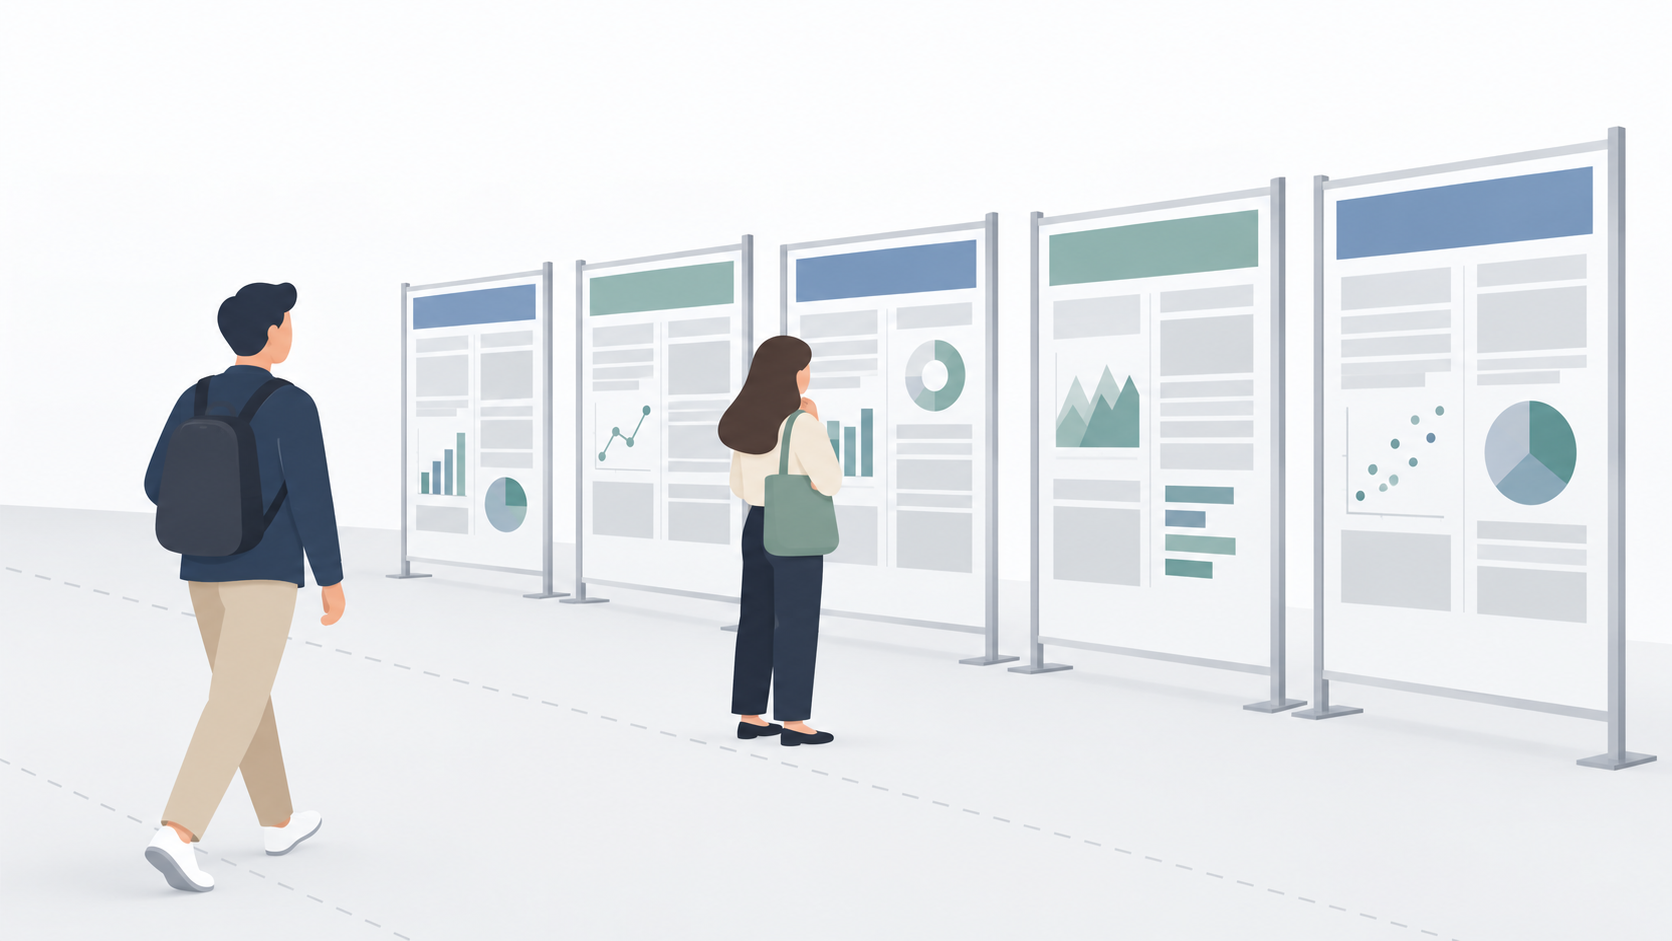
\includegraphics[width=\linewidth]{figures/ch12/ch12-07-poster-hall-distances.png}};
\begin{scope}[x={(img.south east)},y={(img.north west)}]
  \node[font=\footnotesize,fill=white,fill opacity=0.88,text opacity=1,inner sep=2pt] at (0.18,0.12) {约 3--5 m：读标题与主结论};
  \node[font=\footnotesize,fill=white,fill opacity=0.88,text opacity=1,inner sep=2pt] at (0.58,0.12) {约 1 m：读证据与细节};
\end{scope}
\end{tikzpicture}
\caption{海报先被远看，再被近看。示意图，人物与距离不按比例（底图由图像模型生成，距离标签由作者后期叠加；提示词与生成记录见本书仓库）。}\label{fig:ch12-07}
\end{figure}

生成图~\ref{fig:ch12-07} 的无字底图时，同一段英文提示词连续调用了三次：第 1 次生成中地面两条浅灰虚线的倾斜方向分歧明显，第 2 次远距虚线绕到了行走者身后，第 3 次才使两条虚线分别经过左前景行走者脚边与中间驻足阅读者前方，且五块展板只包含蓝青标题色带、两栏浅灰矩形与无字几何图形（底图保留了柔和渐变且展板排占了右侧约四分之三，距离标签由 TikZ 在排版时叠加）。图中直观展示了海报的“两阶段阅读”：通道上约 $3\text{--}5\ \text{m}$ 外的路过者用几秒钟扫视顶部标题带；被吸引而走到约 $1\ \text{m}$ 处的同行则用几分钟依次阅读证据区块与方法细节。

顺应这一过程，我们为 A0 竖版海报设计\textbf{两栏栅格}与\textbf{三层信息结构}（图~\ref{fig:ch12-06}）。

\begin{figure}[htbp]\centering
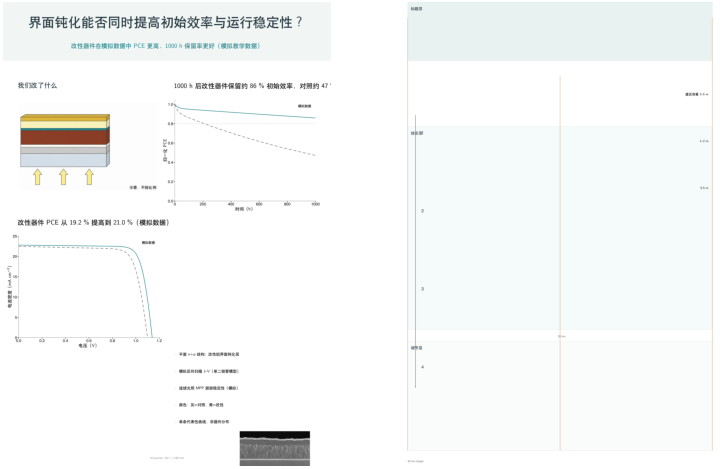
\includegraphics[width=\linewidth]{figures/ch12/ch12-06-a0-poster-layout-zh.pdf}
\caption{A0 竖版海报（$841 \times 1189\ \text{mm}$）的终稿与线框。三层信息分别面向 $3\text{--}5\ \text{m}$、$1\text{--}2\ \text{m}$ 与 $0.5\ \text{m}$ 的阅读；数据图按 $1.5\ \text{m}$ 观看重绘。数据为模拟数据；截面图为模型生成示意。}\label{fig:ch12-06}
\end{figure}

对照图~\ref{fig:ch12-06} 的终稿与线框，A0 竖版海报的布局要点如下：
\begin{enumerate}
\item \textbf{栅格与按栏向下的阅读顺序：}四周留出 $30\ \text{mm}$ 外边距（建议 $\ge 25\ \text{mm}$），顶部设高 $150\ \text{mm}$ 的通栏标题带，主体分为左右两栏，栏间距 $20\ \text{mm}$（建议 $15\text{--}20\ \text{mm}$），单栏净宽 $380.5\ \text{mm}$。阅读顺序按栏从上到下推进（先读左栏上、左栏下，再读右栏上、右栏下，如线框图左侧箭头与编号 \texttt{1}--\texttt{4} 所示），避免观众在近一米宽的展板前左右来回走动（Erren 与 Bourne，2007）。
\item \textbf{三层信息与论文四个面板的重新分工：}
  \begin{itemize}
  \item \textbf{标题层（面向 $3\text{--}5\ \text{m}$）：}顶部浅青灰底色带内，第一行用 $96\ \text{pt}$ 写出研究问题“界面钝化能否同时提高初始效率与运行稳定性？”，第二行用 $44\ \text{pt}$ 青色副标题写出主结论“改性器件在模拟数据中 PCE 更高、$1000\ \text{h}$ 保留率更好（模拟教学数据）”。
  \item \textbf{结论层（面向 $1\text{--}2\ \text{m}$）：}中上部三个核心区块分别对应左栏上“我们改了什么”（器件结构 M1，配 $28\ \text{pt}$“示意，不按比例”）、左栏下效率区块（$J\text{--}V$）和右栏上稳定性区块。每个数据区块顶部配 $48\ \text{pt}$ 结论句，下方数据图按 $1.5\ \text{m}$ 距离专门重绘（轴标题 $32\ \text{pt}$、刻度 $28\ \text{pt}$、线宽 $3.5\ \text{pt}$、右上角“模拟数据” $24\ \text{pt}$）。
  \item \textbf{细节层（面向 $0.5\ \text{m}$）：}右栏下区块用 5 条 $28\ \text{pt}$ 短要点交代平面结构、单二极管模拟、MPP 条件、灰/青颜色定义与单条代表性曲线说明；论文 Figure 2 的面板 b（类 SEM 截面示意 M2）降级移至右下角细节层，并保留 $24\ \text{pt}$ 证据声明。
  \end{itemize}
  按 100\% 尺寸核查图~\ref{fig:ch12-06} 左图的脚本排样时，也能发现送印前需要人工修补的三处细节：一是右栏上稳定性区块的 $48\ \text{pt}$ 结论句较长，单行排布时右端括号在栏边被裁掉一半，应拆成两行或缩至 $44\ \text{pt}$；二是左栏上器件结构图 M1 仅放了无字底图，送印前需补上右侧 $36\ \text{pt}$ 的七层层名标签及数据图内的曲线旁注；三是右下角截面图 M2 左下方的深色标注“模型生成示意，非显微图像”直接叠在深灰基底上对比度不足，应加上浅白半透明底框。
\item \textbf{密度指标与眯眼测试（squint test）：}海报正文总字数建议用“能否在 5 分钟内读完”自测，并保持充足留白。排版后将海报缩至 $12\ \text{cm}$ 高并施加高斯模糊（$\sigma$ 约相当于缩略图上 $1.5\ \text{mm}$），开展\textbf{眯眼测试}（图~\ref{fig:ch12-08}）。
\end{enumerate}

\begin{figure}[htbp]\centering
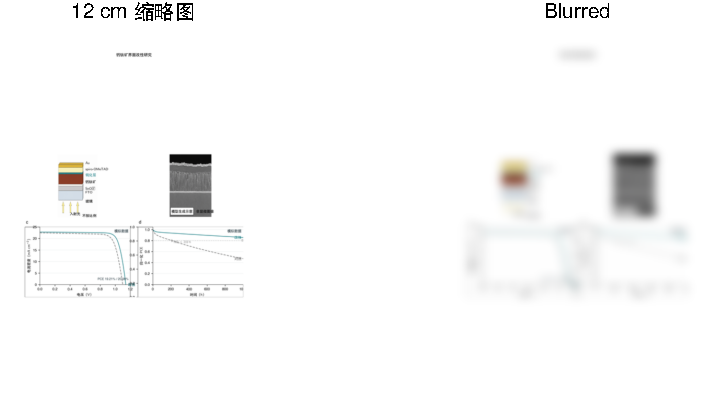
\includegraphics[width=\linewidth]{figures/ch12/ch12-08a-dense-squint-zh.pdf}\\[1mm]
{\footnotesize (a) 拥挤初稿 C0：三栏文字加原样放大的四面板论文组图}\\[3mm]
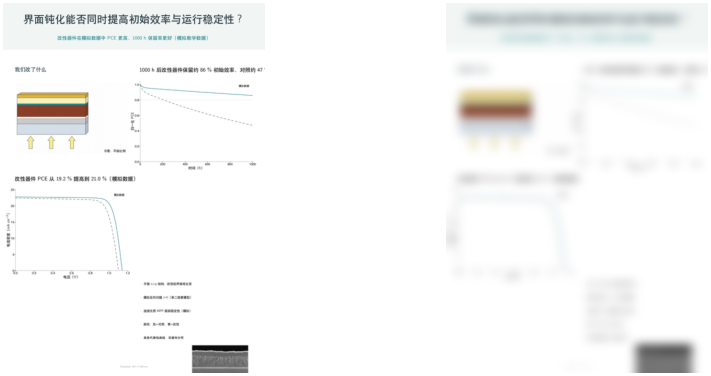
\includegraphics[width=\linewidth]{figures/ch12/ch12-08b-focused-squint-zh.pdf}\\[1mm]
{\footnotesize (b) 分层终稿：顶部标题带、三个结论区块与右下细节层}
\caption{眯眼测试。左：12 cm 高的缩略图；右：模糊后。（a）拥挤初稿只剩均匀灰块；（b）终稿仍能看出标题带和三个区块。}\label{fig:ch12-08}\label{fig:ch12-08a}\label{fig:ch12-08b}
\end{figure}

对比图~\ref{fig:ch12-08}a 与图~\ref{fig:ch12-08}b（注：图~\ref{fig:ch12-08}a 左上方的子图标题因未显式传入中文字体属性出现了三个方框）：拥挤初稿 C0 在顶部只放了 $36\ \text{pt}$ 的小标题“钙钛矿界面改性研究”，上半幅分三栏铺排摘要、引言、方法、结果与讨论、结论五段 $20\ \text{pt}$ 正文（样张共约 230 字），中部把 $174\ \text{mm}$ 宽的论文 Figure 2 等比放大约 $4$ 倍横跨版面（$0.6\ \text{pt}$ 线变成约 $2.4\ \text{pt}$ 尚可，但 $8\ \text{pt}$ 字只变成约 $32\ \text{pt}$，与正文同级而使层次消失）。模糊后，顶部标题与三栏文字化作浅灰影，看不出主结论与区块分工；而终稿（图~\ref{fig:ch12-08}b）模糊后仍能清晰分辨顶部浅青标题带、三个带粗结论横条的区块以及右下细节层。

\section{在 SciDraw AI 中完成三个版本}

在 \scidraw{} 中完成论文、汇报与海报三个版本时，应按具体任务选用对应入口，并分清哪些步骤由平台完成、哪些步骤须由作者在本地软件中复核：
\begin{itemize}
\item \textbf{数据图改画幅与字号重绘（科学可视化 \sdtool{sci-vis}）：}无需重新上传数据表，直接打开第 9 章论文图的历史会话，选中终稿版本继续输入修改指令，即可生成 16:9 汇报版、仅含对照曲线的分步揭示版以及海报图块版。平台支持多轮对话修改、历史版本继续编辑、恢复上一版或原版以及多格式导出。作者需逐项核对数值、坐标范围与颜色语义是否未变，并在 PowerPoint 或海报页面中按实际物理尺寸复核字号（导出格式是否为可编辑真矢量将在第 13 章详述）。
\item \textbf{汇报页框架与海报排版框架（演示模板 \path{/scientific-presentation-templates} 与海报模板）：}演示模板提供学位答辩、会议报告、文献汇报、组会汇报、开题报告等场景的 16:9 PPTX 框架；海报模板提供“经典”“焦点”“四栏”三种风格，尺寸覆盖 A0 竖版、A0 横版、A1、$36\times 48\ \text{in}$、$90\times 120\ \text{cm}$ 与 16:9 电子海报等变体（其中 $72\ \text{in}$ 超宽海报受限于演示软件单页尺寸上限，按 $50\%$ 物理尺寸设计、打印时放大 2 倍，模板内有明确注明）。注意：\textbf{下载 PPTX 模板不等于自动填入内容}，平台目前没有“一键把整篇论文自动排成多页可编辑演示或可编辑海报”的功能，作者需自己将重绘好的图片与结论句排入模板。
\item \textbf{海报整体视觉方向探索（科学海报生成 \path{/scientific-poster-maker}）：}可根据提示词生成单张海报概念图像，也支持导入论文 PDF 生成视觉提示词（目前 PDF 解析仅读取前 5 页及摘要、开头有限文本，并非理解整篇论文）。该工具仅用于开工前比较分栏与配色方向；\textbf{严禁把生成的单张位图直接当成终稿送印}，生成图中的任何文字与假“数据图”一律不用，最终版必须在可编辑模板或脚本中用真实内容排版。
\item \textbf{组图拆解与目标宽度技术检查（组图工具 \sdtool{multi-panel-figure-maker} 与图片检查器 \sdtool{figure-checker}）：}组图工具导出的 PPTX 中，每个面板位图与面板编号文字（\texttt{a}、\texttt{b}……）彼此独立，便于单独提取面板 a 的结构图或删去编号；但面板内部的曲线、坐标轴与文字仍是位图，不可逐根编辑，因此数据面板仍须回 \sdtool{sci-vis} 或脚本按汇报字号重绘。定稿后可用 \sdtool{figure-checker} 按目标物理宽度换算有效分辨率并检查灰度与色觉风险，但字号张角、版面阅读顺序与科学表述仍须由作者用视角公式与眯眼测试自己核查。各工具之间通过下载命名清楚的文件再上传或插入完成交接。
\end{itemize}

\section{完整案例：一项研究的三个版本}

下面将本章钙钛矿太阳能电池界面改性研究从原始材料、三份任务书、修改指令到讲稿、图注与三版一致性核验完整串联起来。

\textbf{一、研究设定与模拟数据参数。}本案例比较平面 n-i-p 钙钛矿太阳能电池的对照器件与界面钝化改性器件，不报告任何真实器件实验结果，所有数据均由标准单二极管模型与给定双指数衰减函数生成。器件自下而上依次为：玻璃 / FTO / $\text{SnO}_2$（约 $30\ \text{nm}$）/ 钙钛矿吸光层（约 $500\ \text{nm}$）/ 界面钝化层（仅改性组，极薄）/ spiro-OMeTAD（约 $200\ \text{nm}$）/ Au（约 $80\ \text{nm}$），不指定具体钙钛矿组分或钝化分子。

四份材料中，M1 为器件结构示意图（不按比例）；M2 为模型生成的类 SEM 截面示意（真实论文中截面形貌必须来自同批器件的实际 SEM 采集并保留原图与比例尺，本书仅因无法公开获取与模拟数据同源的真实照片而用模型图样作版式占位，所有衍生版本均须标明“模型生成示意，非显微图像”）；M3 为 AM1.5G（$100\ \text{mW cm}^{-2}$）、$25\ ^\circ\text{C}$ 下的单二极管模拟 $J\text{--}V$ 曲线（单一反向扫描，未模拟迟滞，迟滞问题参见 Snaith 等，2014；效率理论上限参见 Shockley 与 Queisser，1961），对照组设定 $J_L = 22.5\ \text{mA cm}^{-2}$、目标 $V_{\text{oc}} = 1.10\ \text{V}$、$n = 1.6$、$R_s = 2.5\ \Omega\cdot\text{cm}^2$、$R_{\text{sh}} = 1500\ \Omega\cdot\text{cm}^2$，计算输出 $J_{\text{sc}} = 22.46\ \text{mA cm}^{-2}$、$V_{\text{oc}} = 1.100\ \text{V}$、$\text{FF} = 0.777$、$\text{PCE} = 19.21\%$，改性组设定 $J_L = 22.8\ \text{mA cm}^{-2}$、目标 $V_{\text{oc}} = 1.14\ \text{V}$、$n = 1.5$、$R_s = 2.0\ \Omega\cdot\text{cm}^2$、$R_{\text{sh}} = 3000\ \Omega\cdot\text{cm}^2$，计算输出 $J_{\text{sc}} = 22.78\ \text{mA cm}^{-2}$、$V_{\text{oc}} = 1.140\ \text{V}$、$\text{FF} = 0.808$、$\text{PCE} = 20.98\%$；M4 为连续 1 个太阳光照、最大功率点跟踪、氮气、约 $25\ ^\circ\text{C}$ 下的 $0\text{--}1000\ \text{h}$ 归一化 PCE 模拟序列（稳定性评估与报告共识参见 Khenkin 等，2020），对照组 $y(t) = [1 - 0.08(1 - e^{-t/20})]e^{-t/1500}$ 的 $T_{80} = 210\ \text{h}$、$1000\ \text{h}$ 保留率 $0.47$，改性组 $y(t) = [1 - 0.04(1 - e^{-t/20})]e^{-t/9000}$ 在 $1000\ \text{h}$ 内未降至 $0.80$（$T_{80} > 1000\ \text{h}$）、$1000\ \text{h}$ 保留率 $0.86$。

\textbf{二、三份任务书。}三个版本各自遵循如下任务书。

任务书 A（论文版 Figure 2）：
\begin{Prompt}
【用途与读者】论文 Figure 2，读者为光伏/材料方向同行，单独阅读，节奏由读者控制。
【一句话目标】读者能看出改性器件在初始效率和 1000 h 稳定性上都优于对照，并能找到 Jsc、Voc、FF、PCE 和 T80。
【面板】a 器件结构；b 截面图样（模型生成示意）；c J–V；d 归一化 PCE–时间。
【尺寸】双栏 174 mm 宽，面板内字号 8 pt，面板字母 10 pt 粗体小写。
【不可改变】全部数值来自统一计算结果文件；颜色语义：对照灰 #6E6E6E 虚线，改性青 #1B7F86 实线。
【标注】c、d 为模拟数据；b 为模型生成示意，非显微图像；a 不按比例。
\end{Prompt}

任务书 B（组会 / 会议汇报版，3 页 16:9）：
\begin{Prompt}
【用途与读者】10 分钟组会报告中的结果部分，约 3 分钟；听众为课题组成员与相近方向同行；
投影屏幕高约 2 m，最后一排约 10–12 m；节奏由讲者控制。
【一句话目标】听众在 3 页内依次理解：器件做了什么改动 -> 初始效率提高了多少 -> 稳定性改善了多少。
【每页】
  第 1 页 标题句：“只在钙钛矿/空穴层界面加了一层钝化”。器件结构（M1）放大，钝化层高亮；
          类 SEM 示意不放入正文页（放备用页，标注保留）。
  第 2 页 标题句：“改性器件 PCE 从 19.2 % 提高到 21.0 %（模拟数据）”。J–V 分两步揭示：
          先坐标轴+对照，再加改性；关键参数用直接标注与简表，不用独立图例。
  第 3 页 标题句：“1000 h 后改性器件保留约 86 % 初始效率，对照约 47 %（模拟数据）”。
          稳定性曲线，标出 0.8 参考线与对照 T80。
【版式】16:9，33.867 x 19.05 cm；正文与刻度 >= 20 pt，轴标题 >= 24 pt，页标题 32–36 pt；线宽 >= 2.5 pt；无面板字母。
【不可改变】数值、轴物理量与单位、颜色语义、“模拟数据”标注。
【验收】在笔记本屏幕上把页面缩到 1/4 大小，标题句与轴标签仍可读；每页数值与结果文件一致。
\end{Prompt}

任务书 C（A0 竖版海报）：
\begin{Prompt}
【用途与读者】学术会议海报展区，A0 竖版 841 x 1189 mm；路过者在 2–5 m 外决定是否停留，
停留者在 0.5–1.5 m 阅读 3–5 分钟；作者不一定在场。
【一句话目标】从 3 m 外读到研究问题与主结论；走近后依次读到“做了什么—效率—稳定性”三块证据和必要方法。
【层次】标题层：研究问题+主结论（标题 >= 90 pt）；结论层：3 个区块，每块一句结论（>= 44 pt）+ 一张图；
细节层：方法要点、参数、参考文献、二维码（正文 >= 28 pt，最小 24 pt）。
【栅格】2 栏，外边距 30 mm，栏间距 20 mm；阅读顺序：标题 -> 左栏上（结构）-> 左栏下（J–V）
-> 右栏上（稳定性）-> 右栏下（方法、截面示意、参考）。
【图】数据图按 1.5 m 观看重绘（刻度 >= 28 pt，线宽 >= 3 pt），不是论文图放大；类 SEM 示意放细节层。
【不可改变】同任务书 B。
【验收】缩到 12 cm 高的缩略图上能分辨 3 个区块和主结论；1:1 打印 A4 局部样张在 1.5 m 处可读。
\end{Prompt}

\textbf{三、可复制的修改指令与海报版式提示词。}对 \sdtool{sci-vis} 中第 9 章的 $J\text{--}V$ 会话（选择论文终稿那一版继续修改），输入如下指令：
\begin{Prompt}
在保持全部数据点、两组颜色（对照 #6E6E6E、改性 #1B7F86）、横轴 0–1.2 V、纵轴 0–25 mA/cm2 不变的前提下，
生成一个用于 16:9 幻灯片的版本：
1. 画布 16:9，图占画面左侧约 60%；
2. 坐标刻度字号相当于 20 pt、轴标题 24 pt（按 33.867 cm 宽的幻灯片计算）；线宽 3 pt；
3. 删除图例，在曲线空白处直接标注“对照”“改性”；
4. 在图内右上角写“模拟数据”；
5. 不添加任何新的数值、误差线或显著性标记。
另外输出一个只有对照曲线的版本（坐标轴、标注相同），用于分步揭示。
\end{Prompt}

生成后需核对两版坐标范围是否完全一致（叠放切换时曲线不能跳动）、标注数值是否与结果文件一致，以及工具是否擅自改动了颜色或平滑了曲线。制作海报版数据图时，只需把上述指令改为“按 A0 海报中宽 $380\ \text{mm}$ 的图块、$1.5\ \text{m}$ 观看距离：刻度 $28\ \text{pt}$、轴标题 $32\ \text{pt}$、线宽 $3.5\ \text{pt}$”。

若使用 \texttt{/scientific-poster-maker} 生成海报版式与视觉方向参考，可输入如下英文提示词：
\begin{Prompt}
A0 portrait academic poster layout for a materials science study, two columns,
clear title band across the top, three large figure blocks with generous white space,
a narrow footer band. Clean flat design, white background, one accent color teal.
Use simple placeholder rectangles for figures and grey bars for text;
do not render any readable words.
\end{Prompt}

\textbf{四、讲稿要点与海报区块图注。}汇报第 2 页（图~\ref{fig:ch12-04} 的 2a $\rightarrow$ 2b，约 40 秒）配套讲稿：
\begin{BookNote}
“先看坐标：横轴是电压，纵轴是电流密度，曲线和两轴围成的矩形越‘方’，填充因子越高。灰线是对照——（点击）青线是改性器件。开路电压从 $1.10\ \text{V}$ 提高到 $1.14\ \text{V}$，填充因子从 $0.78$ 提高到 $0.81$，效率从 $19.2\%$ 到 $21.0\%$。这些是模拟数据，用来说明表达方法。”
\end{BookNote}

海报左栏下 $J\text{--}V$ 区块配套图注：
\begin{BookNote}
改性器件的开路电压与填充因子较高。模拟反向扫描 $J\text{--}V$ 曲线（单二极管模型），AM1.5G，$100\ \text{mW cm}^{-2}$；每组一条代表性曲线，不代表器件间分布。
\end{BookNote}

\textbf{五、三版一致性核验。}最终交付前，对照表~\ref{tab:ch12-02} 逐项核验三个版本的一致性。

\begin{table}[htbp]\centering\footnotesize
\setlength{\tabcolsep}{3pt}
\renewcommand{\arraystretch}{1.15}
\caption{论文版、汇报版与海报版的三版一致性核验表。}\label{tab:ch12-02}
\begin{tabularx}{\linewidth}{@{}>{\raggedright\arraybackslash}p{26mm}YYY>{\raggedright\arraybackslash}p{16mm}@{}}
\toprule
\textbf{检查项} & \textbf{论文版} & \textbf{汇报版} & \textbf{海报版} & \textbf{是否一致} \\
\midrule
$J_{\text{sc}}$ / $V_{\text{oc}}$ / $\text{FF}$ / $\text{PCE}$（两组） & 结果表与面板 c 标注 & 第 2 页标题与右侧小表 & 左栏下 $J\text{--}V$ 区块 & 逐项一致 \\
$T_{80}$（对照 $\approx 210\ \text{h}$）、$1000\ \text{h}$ 保留率（$0.47$ / $0.86$） & 结果表与面板 d 标注 & 第 3 页标题与图内标注 & 右栏上稳定性区块 & 逐项一致 \\
轴物理量、单位、范围 & $0\text{--}1.2\ \text{V}$；$0\text{--}25\ \text{mA cm}^{-2}$；$0\text{--}1000\ \text{h}$ & 同论文版（2a/2b 完全锁定） & 同论文版 & 是（改变须说明） \\
颜色与线型语义 & 灰虚线=对照，青实线=改性 & 同论文版 & 同论文版 & 是 \\
“模拟数据”标注 & 图注及面板 c、d 右上角 & 每张数据页标题与图内 & 标题带、每张数据图内及细节层 & 是 \\
“模型生成示意，非显微图像” & 图注及面板 b 左下角 & 备用页图内 & 右栏下细节层图内 & 是 \\
新增内容 & — & 无新数值或伪造统计 & 无新数值或伪造统计 & 是 \\
\bottomrule
\end{tabularx}
\end{table}

\section{AI 在这一步能做什么与不能做什么}

把论文配图改造成口头汇报和学术海报时，AI 与作者的职责边界汇总于表~\ref{tab:ch12-01}。

\begin{table}[htbp]\centering\footnotesize
\setlength{\tabcolsep}{3pt}
\renewcommand{\arraystretch}{1.15}
\caption{在汇报与海报制作环节中 AI 能做什么、不能做什么与作者必须核对的内容。}\label{tab:ch12-01}
\begin{tabularx}{\linewidth}{@{}>{\raggedright\arraybackslash}p{18mm}YYY@{}}
\toprule
\textbf{环节} & \textbf{AI 能做} & \textbf{AI 不能做} & \textbf{作者要核对} \\
\midrule
拆分故事 & 根据作者给出的结论句草拟页面顺序、页标题候选 & 判断哪个结果是研究的主要贡献；替你决定删掉哪些证据 & 每页标题句有数据支撑、限定条件没丢（“模拟”“单条曲线”） \\
数据图重绘 & 在 \sdtool{sci-vis} 中按新画幅、字号、线宽重绘；生成分步揭示用的子集版本 & 保证字号在最终投影/打印尺寸下精确；保证没有顺手改动坐标或平滑曲线 & 数值、轴范围、颜色语义与论文版逐项一致；字号在 PowerPoint 实际尺寸复核 \\
海报版式 & 用 \path{/scientific-poster-maker} 生成版式与视觉方向参考；提供 PPTX 海报模板 & 生成可直接印刷、文字正确、数据真实的海报；把论文自动排进模板 & 生成图中的文字与“数据”一律不用；最终版在可编辑模板中排 \\
演示文件 & 提供多种 PPTX 演示模板；组图可导出面板分离的 PPTX & 把论文内容自动排成多页可编辑演示；让面板内曲线可逐条编辑 & 模板只是框架；面板内部是位图 \\
讲稿与图注 & 草拟讲稿与海报短图注 & 编造样本量、统计或未给出的条件 & 讲稿中的每个数字回到结果表；证据状态标注在每个版本都保留 \\
检查 & \sdtool{figure-checker} 按目标宽度换算有效分辨率、色觉风险等 & 判断字号、版面层次、阅读顺序或科学正确性 & 用第 12.2 节的换算和眯眼测试自己查 \\
\bottomrule
\end{tabularx}
\end{table}

\section{本章检查清单}

\begin{itemize}
\item 三个版本各有一份任务书，写明观看距离、时间与节奏控制者。
\item 用视角换算确定了每个版本的最小字号与线宽，并在实际尺寸（PowerPoint 页面 / A0 PDF）中复核。
\item 汇报每页只有一个结论句和一组证据；逐步揭示的各帧坐标范围相同。
\item 汇报和海报中的数据图是重绘的，不是论文图放大或截图。
\item 去掉了面板字母和需要来回对照的图例，改为直接标注。
\item 海报有标题层、结论层、细节层；缩略加模糊后仍能看出主要区块。
\item 三版一致性表逐项核对通过：数值、单位、轴范围、颜色语义一致。
\item “模拟数据”“模型生成示意，非显微图像”“示意，不按比例”等证据标注出现在每一个衍生版本的画面上，而不只在论文图注里。
\item 没有使用海报生成图中的文字或数据；没有把模板下载说成自动排版。
\item 各步输入与重绘文件已按版本妥善归档保存。
\end{itemize}

\section{练习}

\begin{enumerate}
\item \textbf{（算一算：纸笔）}你的报告厅屏幕高 $1.6\ \text{m}$，最后一排距屏幕 $14\ \text{m}$。（a）与 $9\ \text{pt}@40\ \text{cm}$ 相同张角时，16:9 幻灯片正文最小约多少 $\text{pt}$？（b）若会议海报正文要在 $1.8\ \text{m}$ 处读到，至少多少 $\text{pt}$？\\
{\footnotesize \textbf{参考答案：}（a）$D/H = 8.75$，$\text{pt} \approx 0.00785 \times 8.75 \times 540 \approx 37\ \text{pt}$（说明这个会场需要比“$24\ \text{pt}$ 下限”更大的字，或减少每页文字）；（b）$9 \times 1.8 / 0.4 = 40.5\ \text{pt}$。}

\item \textbf{（拆一张自己的组图：\scidraw{} 实操）}选你论文中的一张多面板图，写出它回答的 2--3 个子问题，各写一句结论作为页标题。在 \sdtool{sci-vis} 打开对应数据图的历史会话（或重新上传数据），用第 12.6 节的修改指令格式生成 16:9 版本和分步揭示版本；把两版坐标范围、数值和颜色做成一致性表。提交：页面 PNG、修改指令原文、一致性表。

\item \textbf{（眯眼测试）}下载本章图~\ref{fig:ch12-06} 的海报 PDF 和你自己（或同学）的一张海报，缩到 $12\ \text{cm}$ 高并模糊（或站在 $3\ \text{m}$ 外拍照）。写出：能否看出研究问题、主结论和 3 个区块；若不能，列出三条可执行的修改指令（例如“把‘结果’改为结论句‘……’”，而不是“让海报更清楚”）。
\end{enumerate}

\section*{参考文献}

\begin{itemize}
\item Bourne, P. E. (2007). Ten simple rules for making good oral presentations. \textit{PLoS Computational Biology}, 3(4), e77. \url{https://doi.org/10.1371/journal.pcbi.0030077}
\item Erren, T. C., \& Bourne, P. E. (2007). Ten simple rules for a good poster presentation. \textit{PLoS Computational Biology}, 3(5), e102. \url{https://doi.org/10.1371/journal.pcbi.0030102}
\item Khenkin, M. V., Katz, E. A., Abate, A., Bardizza, G., Berry, J. J., Brabec, C., \ldots{} Lira-Cantu, M. (2020). Consensus statement for stability assessment and reporting for perovskite photovoltaics based on ISOS procedures. \textit{Nature Energy}, 5, 35--49. \url{https://doi.org/10.1038/s41560-019-0529-5}
\item Naegle, K. M. (2021). Ten simple rules for effective presentation slides. \textit{PLOS Computational Biology}, 17(12), e1009554. \url{https://doi.org/10.1371/journal.pcbi.1009554}
\item Rougier, N. P., Droettboom, M., \& Bourne, P. E. (2014). Ten simple rules for better figures. \textit{PLoS Computational Biology}, 10(9), e1003833. \url{https://doi.org/10.1371/journal.pcbi.1003833}
\item Shockley, W., \& Queisser, H. J. (1961). Detailed balance limit of efficiency of p-n junction solar cells. \textit{Journal of Applied Physics}, 32(3), 510--519. \url{https://doi.org/10.1063/1.1736034}
\item Snaith, H. J., Abate, A., Ball, J. M., Eperon, G. E., Leijtens, T., Noel, N. K., \ldots{} Wiesner, U. (2014). Anomalous hysteresis in perovskite solar cells. \textit{The Journal of Physical Chemistry Letters}, 5(9), 1511--1515. \url{https://doi.org/10.1021/jz500113x}
\end{itemize}

\chapter{检查、导出与可追溯交付}

材料学博士生小周终于把钙钛矿太阳能电池界面钝化论文的稿件投了出去。两周后，稿件没有进入同行评审，而是收到了一封来自期刊编辑部的技术退回邮件。退回理由有两条：第一，论文的 Figure 2 虽然以 PDF 格式上传，但其中的电流密度—电压（J–V）曲线与稳定性曲线在出版系统预检时被识别为低分辨率位图，而非矢量线条图；第二，面板 a 器件结构示意图中的层名文字在缩放到期刊栏宽后，字号掉到了 5 pt，低于该期刊要求的 7 pt 下限。

同一天下午，一位习惯打印读论文的合作者拿着黑白激光打印稿走进实验室，指着 Figure 2 下排的两条实线问小周：“灰度打印出来两条线深浅完全一样，哪条是对照组，哪条是钝化改性组？”紧接着，接手课题的师妹也发来消息，想把 Figure 2c 的数据重画成组会幻灯片，却发现课题组网盘里存着 \texttt{fig2\_final.png}、\texttt{fig2\_final2.pdf} 和 \texttt{fig2\_ok\_zh.png} 三个文件，谁也说不清哪一个才对应投稿版本，更找不到当时生成示意底图的提示词和修改记录。

这些问题没有一个涉及钙钛矿界面钝化本身的物理机制，却足以推迟稿件送审，并让审稿人和读者误读实验与模拟结果。一张科研图只有同时通过\textbf{印前技术检查}（有效分辨率、最终字号与线宽、矢量与容器结构、色彩与灰度可区分性）并附带\textbf{可追溯的交付档案}，才算真正完成。本章将交付前的最后一轮检查拆解为可以逐条照单执行的算式、命令与核验动作。

\section{物理尺寸、像素与有效分辨率}

在期刊投稿系统和课题组日常交流中，“这张图是不是 300 dpi”是最常被问到、也最容易产生误解的一句话。要算清分辨率，必须先把三个彼此独立的物理量区分开来：

\begin{enumerate}
\item \textbf{像素数（pixel dimensions）：}图像文件内部横向与纵向究竟包含多少个像素格，例如 $1920 \times 1080\ \text{px}$ 或 $2008 \times 1417\ \text{px}$。这是位图文件真正拥有的采样网格数量。
\item \textbf{物理尺寸（physical size）：}图片最终印在期刊页面、学位论文或海报上的实际宽度与高度，通常以毫米（mm）或英寸（$\text{in}$，$1\ \text{in} = 25.4\ \text{mm}$）计量，例如单栏宽 $85\ \text{mm}$、双栏宽 $180\ \text{mm}$ 或 $190\ \text{mm}$。
\item \textbf{有效分辨率（effective resolution）：}当这张位图被缩放到最终物理尺寸时，每英寸宽度内实际分配到多少个像素，单位写作 ppi（pixels per inch，常与印刷设备指标 dpi 混称）。
\end{enumerate}

这三个量之间只有一条换算关系（图~\ref{fig:ch13-01}）：
\begin{gather*}
\text{有效分辨率（ppi）} = \frac{\text{横向像素数（px）}}{\text{最终物理宽度（mm）} \div 25.4} \\[3pt]
\text{所需横向像素数（px）} = \frac{\text{最终物理宽度（mm）}}{25.4} \times \text{目标分辨率（dpi）}
\end{gather*}

\begin{figure}[htbp]\centering
\makebox[\linewidth][c]{% FIG ch13-01 pixels, physical size, effective resolution (Chinese)
% 栏宽按 1:2 绘制（栏宽 1 mm = 本页 0.5 mm），与英文图同一版式。
\begin{tikzpicture}[x=1mm, y=1mm, font=\sffamily\fontsize{8}{10}\selectfont, text=BookInk,
    >=Stealth]
  \tikzset{
    lbl/.style={inner sep=0pt, outer sep=0pt, anchor=south west},
    result/.style={inner sep=0pt, outer sep=0pt, anchor=north west},
    tick/.style={inner sep=0.4pt, outer sep=0pt, anchor=north},
    takeaway/.style={draw=BookTeal, line width=0.6pt, fill=white, rounded corners=1.2pt,
      inner sep=1.8mm, align=center, text width=122mm, font=\sffamily\fontsize{8}{10.5}\selectfont},
  }

  % 同一个位图文件
  \draw[BookRule, line width=0.6pt, fill=BookPale, rounded corners=1.2pt]
    (0.6, 43.0) rectangle (30.0, 76.8);
  \begin{scope}
    \clip (6.2, 63.2) rectangle (24.2, 73.325);
    \fill[white] (6.2, 63.2) rectangle (24.2, 73.325);
    \foreach \i in {0,...,15} {
      \foreach \j in {0,...,8} {
        \pgfmathparse{mod(\i+\j,2) ? 18 : 8}
        \fill[BookTeal!\pgfmathresult]
          (6.2+1.125*\i, 63.2+1.125*\j) rectangle ++(1.125, 1.125);
      }
    }
  \end{scope}
  \draw[BookRule, line width=0.4pt] (6.2, 63.2) rectangle (24.2, 73.325);
  \node[align=center, inner sep=0pt, anchor=center] at (15.3, 53.2)
    {{\fontsize{9}{11}\selectfont 文件}\\[2.5pt]1920 × 1080\,像素};

  % 两条宽度条的共同起点。85 mm -> 42.5 mm；180 mm -> 90 mm。
  \def\xO{36.2}
  \def\sS{0.5}

  \node[lbl] at (\xO, 73.4) {单栏 85\,mm};
  \fill[BookTeal] (\xO, 68.4) rectangle ({\xO+85*\sS}, 71.8);
  \node[result] at (\xO, 66.6) {1920 ÷ (85 ÷ 25.4) ≈ \textbf{574\,ppi}};

  \node[lbl] at (\xO, 56.6) {双栏 180\,mm};
  \fill[BookTeal] (\xO, 51.6) rectangle ({\xO+180*\sS}, 55.0);
  \node[result] at (\xO, 49.8) {1920 ÷ (180 ÷ 25.4) ≈ \textbf{271\,ppi}};

  \draw[BookInk, line width=0.55pt, ->] (30.0, 70.1) -- (\xO, 70.1);
  \draw[BookInk, line width=0.55pt, ->] (30.0, 53.3) -- (\xO, 53.3);

  % 与宽度条同一比例的标尺
  \draw[BookInk, line width=0.7pt] (\xO, 41.2) -- ({\xO+180*\sS}, 41.2);
  \foreach \mm/\lab in {0/0, 85/85, 180/180\,mm} {
    \draw[BookInk, line width=0.55pt] ({\xO+\mm*\sS}, 41.2) -- ({\xO+\mm*\sS}, 39.6);
    \node[tick] at ({\xO+\mm*\sS}, 39.3) {\lab};
  }
  \node[inner sep=0pt, outer sep=0pt, anchor=north west] at (0.6, 34.6)
    {同一比例尺（栏宽 1\,mm = 本页 0.5\,mm）};

  \node[takeaway, anchor=north west] at (0.6, 29.2) {%
    有效分辨率 = 像素数 ÷（宽度 mm ÷ 25.4）\\[2pt]
    改动文件里的 dpi 标签不改变像素数};
\end{tikzpicture}
}
\caption{同一文件放到不同宽度，有效分辨率不同。有效分辨率由像素数和最终印刷宽度决定，与文件中记录的 dpi 标签无关。}\label{fig:ch13-01}
\end{figure}

理解这条算式之后，两个常见的修图误区就不攻自破了。

第一个误区是\textbf{把“文件头里的 dpi 标签”当成有效分辨率}。PNG、TIFF 和 JPEG 的元数据里通常存着一个水平与垂直 dpi 数字（例如许多截图或绘图软件默认写入 72 dpi 或 96 dpi）。如果作者在图像处理软件里取消勾选“重新采样（Resample）”，只把数字从 72 改成 300，文件里的像素总数一格也没有增加；一旦排版系统把这张图拉宽到期刊双栏宽度，画面依然会因为像素不足而发虚。反过来，哪怕文件头写着 72 dpi，只要它横向有 $2126\ \text{px}$，放进 $180\ \text{mm}$ 双栏版面时的有效分辨率就是实打实的 $300\ \text{ppi}$。

第二个误区是\textbf{脱离目标版面宽度谈分辨率}。如图~\ref{fig:ch13-01} 所示，同样一张 $1920 \times 1080\ \text{px}$ 的高清位图，放进 $85\ \text{mm}$ 单栏（约 $3.35\ \text{in}$）时，有效分辨率高达 $1920 \div (85 \div 25.4) \approx 574\ \text{ppi}$，足以满足大多数期刊对照片和组合图的要求；但如果把同一文件直接拉满 $180\ \text{mm}$ 双栏（约 $7.09\ \text{in}$），有效分辨率就会立刻降到 $1920 \div (180 \div 25.4) \approx 271\ \text{ppi}$，连 $300\ \text{dpi}$ 的照片底线都达不到。同理，一张 $1024\ \text{px}$ 宽的图像放在 $85\ \text{mm}$ 单栏时约为 $306\ \text{ppi}$，一旦放到 $180\ \text{mm}$ 双栏就只剩 $144\ \text{ppi}$，肉眼即可看出明显的锯齿与模糊。

表~\ref{tab:ch13-px-calc} 给出了常见期刊栏宽与目标分辨率对应的横向像素数，以及常见图像像素宽度在不同栏宽下的有效分辨率。在新建画布或设置导出参数前，按表或公式手算一次只需十秒钟。

\begin{table}[htbp]\centering\footnotesize
\setlength{\tabcolsep}{4pt}
\renewcommand{\arraystretch}{1.18}
\caption{常见版面宽度下的目标像素数与常见像素宽度的有效分辨率换算。}\label{tab:ch13-px-calc}
\begin{tabularx}{\linewidth}{@{}>{\raggedright\arraybackslash}p{30mm}>{\raggedright\arraybackslash}p{26mm}>{\raggedright\arraybackslash}p{28mm}Y@{}}
\toprule
\textbf{计算方向} & \textbf{版面或文件参数} & \textbf{目标要求或条件} & \textbf{换算算式与结果} \\
\midrule
由宽度与 dpi 算像素 & 单栏 $85\ \text{mm}$（$3.35\ \text{in}$） & 照片 $300\ \text{dpi}$ / 组合 $600\ \text{dpi}$ & $85 \div 25.4 \times 300 \approx 1004\ \text{px}$；$\times 600 \approx 2008\ \text{px}$ \\
由宽度与 dpi 算像素 & 双栏 $180\ \text{mm}$（$7.09\ \text{in}$） & 照片 $300\ \text{dpi}$ / 组合 $600\ \text{dpi}$ & $180 \div 25.4 \times 300 \approx 2126\ \text{px}$；$\times 600 \approx 4252\ \text{px}$ \\
由宽度与 dpi 算像素 & 双栏 $190\ \text{mm}$（$7.48\ \text{in}$） & Elsevier 线条图 $1000\ \text{dpi}$ & $190 \div 25.4 \times 1000 \approx 7480\ \text{px}$（组合图 $500\ \text{dpi} \approx 3740\ \text{px}$） \\
由像素与宽度算 ppi & 横向 $1920\ \text{px}$ 文件 & 放 $85\ \text{mm}$ 单栏 / $180\ \text{mm}$ 双栏 & 单栏：$1920 \div 3.35 \approx 574\ \text{ppi}$；双栏：$1920 \div 7.09 \approx 271\ \text{ppi}$ \\
由像素与宽度算 ppi & 横向 $1024\ \text{px}$ 文件 & 放 $85\ \text{mm}$ 单栏 / $180\ \text{mm}$ 双栏 & 单栏：$1024 \div 3.35 \approx 306\ \text{ppi}$；双栏：$1024 \div 7.09 \approx 144\ \text{ppi}$ \\
\bottomrule
\end{tabularx}
\end{table}

发现手头位图的像素数不够时，很多人的第一反应是用软件把图像“插值放大”到目标像素数。图~\ref{fig:ch13-02} 用本章钙钛矿案例的模拟 J–V 曲线（目标尺寸 $85 \times 60\ \text{mm}$）展示了“低分辨率导出后插值放大”与“直接按目标分辨率输出”的对比。

\begin{figure}[htbp]\centering
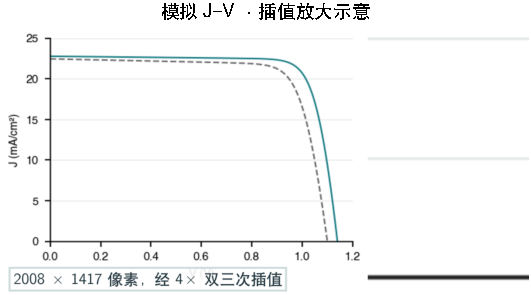
\includegraphics[width=85mm]{figures/ch13/ch13-02a-upsampled-zh.pdf}\\[1.5mm]
{\footnotesize (a) 先按 150 dpi 栅格化（$502 \times 354\ \text{px}$），再经 $4\times$ 双三次插值放大到 $2008 \times 1417\ \text{px}$}\\[3mm]
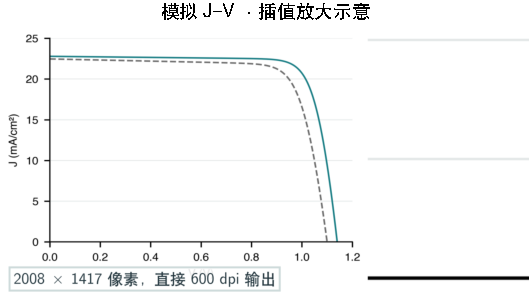
\includegraphics[width=85mm]{figures/ch13/ch13-02b-native-zh.pdf}\\[1.5mm]
{\footnotesize (b) 直接按 600 dpi 输出（$2008 \times 1417\ \text{px}$）}
\caption{像素数相同，信息量不同。(a) 150 dpi 输出后插值放大到 600 dpi；(b) 直接按 600 dpi 输出。局部为 8 倍放大。数据为模拟数据。}\label{fig:ch13-02}
\end{figure}

仔细对比图~\ref{fig:ch13-02} 的上下两幅图：两份文件的像素数完全相同，都是 $2008 \times 1417\ \text{px}$，如果只靠自动化脚本查像素尺寸，两者都会显示“达到 $600\ \text{ppi}$”。但看实际画面就能发现明显差别：在图~\ref{fig:ch13-02}a 左侧整图中，刻度数字（\texttt{0.0}–\texttt{1.2}、\texttt{0}–\texttt{25}）、纵轴标题“\texttt{J (mA/cm²)}”以及灰色虚线与青色实线都发虚发软；右侧 8 倍放大局部截取了底部黑色坐标轴线与两条浅灰水平网格线，可以看到图~\ref{fig:ch13-02}a 的黑线与网格线上下两侧都拖着一层模糊的灰边（那是 $502 \times 354\ \text{px}$ 低分辨率像素被双三次插值平滑过渡后留下的伪影），而图~\ref{fig:ch13-02}b 直接在 $600\ \text{dpi}$ 下渲染，无论左侧文字还是右侧 8 倍放大的轴线边缘都干净锐利。

顺带指出图~\ref{fig:ch13-02} 画面本身暴露出的两处排版细节：一是左下角标注像素数的白底浅框放在了固定相对坐标处，向上遮挡了横轴标题“\texttt{V (V)}”的上半截；二是右侧 8 倍放大框在纵向裁切时只保留了水平网格线与底轴，没有把右侧曲线拐点与坐标文字一起框进来。这也提醒我们，自己在做 $800\%$ 放大检查时，不要只盯着空白处的水平线，而要把放大镜移到曲线拐点、斜线段和上下标文字处逐一查看。

数学插值放大（双线性、双三次或 Lanczos）只是在相邻旧像素之间按函数关系填补平滑过渡的新像素，\textbf{只增加文件体积，不增加任何真实空间信息}。比传统插值更需要警惕的是\textbf{生成式 AI 超分辨率放大}。如果把分辨率偏低的扫描电镜（SEM）照片、荧光显微图像或蛋白印迹条带放进 AI 放大工具，模型确实会让边缘看起来变“锐利”，但这种锐利是神经网络根据训练集中看过的纹理猜出来的——它可能把原本模糊的晶界补成清晰的柱状晶粒，或者在背景噪声里画出根本不存在的微孔。正如第 8 章所强调的，原始实验图像属于观测证据，\textbf{严禁对作为科学证据的实验图像使用生成式 AI 放大或重绘}。若实验原图有效分辨率不足，合规做法只有两条：要么回到原始采集文件重新导出全分辨率原图，要么缩小该面板在组图中的物理宽度并在处理记录中如实写明原图像素数。

在使用 \scidraw{} 时需分清两类工具的处理机制：通用图像转换工具的 dpi 档位映射到固定最大像素边长，当原图像素不足时可能调用 AI 放大，因此绝不能用它给实验原图“补分辨率”；而组图工具（\sdtool{multi-panel-figure-maker}）的导出引擎严格按目标版面的物理毫米尺寸与设定 dpi 换算画布，并在导出的处理记录（\texttt{processing-log}）中如实记录每个面板的原始像素、排版毫米宽度与最终有效分辨率。

\section{在最终宽度下检查字号与线宽}

搞清楚有效分辨率之后，第二个在技术初审和同行阅读中高频翻车的指标是\textbf{最终印刷字号与线宽}。

许多研究生用 Python（Matplotlib）、R、Origin 或 PowerPoint 画图时，习惯在软件默认画布尺寸下看着屏幕调字号：屏幕上看 $10\ \text{pt}$ 的坐标轴文字清清楚楚，导出后塞进 Word 或 LaTeX 的单栏里，印出来却小得像蚂蚁。原因很简单：把宽图整体缩放到较窄的期刊栏宽时，图中所有文字的字号和线条的粗细都会按完全相同的几何比例线性缩小：
\[
\text{最终字号（pt）} = \text{作图时设定的字号（pt）} \times \frac{\text{最终版面宽度（mm）}}{\text{作图画布宽度（mm）}}
\]

我们拿两个最常见的作图场景算一笔账：
\begin{itemize}
\item \textbf{Matplotlib 默认宽画布缩放：}以第 1 章与第 5 章使用的配对比较图为例，原始脚本画布宽度为 $7.3\ \text{in}$（即 $7.3 \times 25.4 \approx 185.4\ \text{mm}$），坐标轴与标签字号设为 $10\ \text{pt}$。如果这张图按双栏 $180\ \text{mm}$ 满宽排版，最终字号是 $10 \times 180 \div 185.4 \approx 9.7\ \text{pt}$，完全合规；可一旦在定稿时决定把它改放进 $85\ \text{mm}$ 单栏（或作为双栏四面板组图的半栏面板），缩放比例就变成 $85 \div 185.4 \approx 0.458$，原本 $10\ \text{pt}$ 的文字印出来只剩 $10 \times 85 \div 185.4 \approx 4.6\ \text{pt}$（精确值 $4.58\ \text{pt}$）。这不仅低于 Elsevier 要求的最终 $7\ \text{pt}$ 和 PLOS ONE 要求的 $8\ \text{pt}$，甚至跌破了 Nature 允许的 $5\ \text{pt}$ 绝对下限。
\item \textbf{PowerPoint 宽屏画布缩放：}PowerPoint 默认 16:9 宽屏幻灯片宽度为 $33.867\ \text{cm}$（$338.7\ \text{mm}$）。不少同学喜欢在满屏幻灯片上用 $24\ \text{pt}$ 或 $18\ \text{pt}$ 画流程图，导出图片后缩放到 $85\ \text{mm}$ 单栏宽时，缩放比例约为 $85 \div 338.7 \approx 0.251$：画布上看似很大的 $24\ \text{pt}$ 文字会被缩成 $6.0\ \text{pt}$，而 $18\ \text{pt}$ 的注释则会缩成 $4.5\ \text{pt}$。
\end{itemize}

图~\ref{fig:ch13-03} 把配对比较数据（8 个模拟对象，其中 \texttt{SIM04} 从前测 18 降至后测 17）的两种做法按\textbf{实际 $85\ \text{mm}$ 物理宽度}直接印在书页上，让你不用算公式就能直观对比 $4.6\ \text{pt}$ 与 $7\ \text{pt}$ 的阅读感受。

\begin{figure}[htbp]\centering
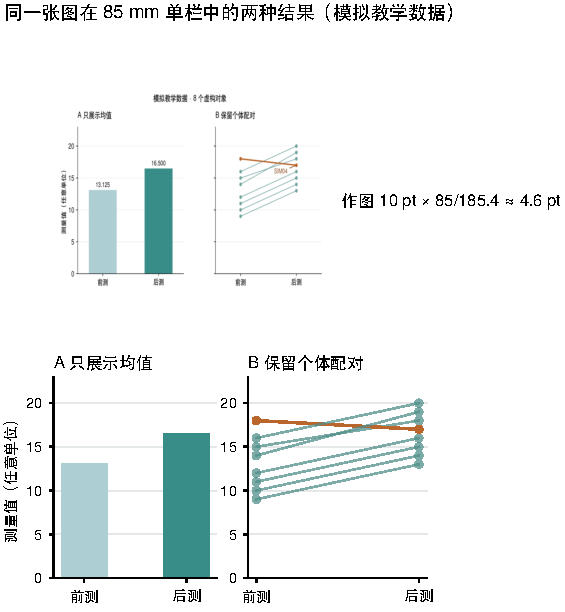
\includegraphics[width=85mm]{figures/ch13/ch13-03-text-at-final-width-zh.pdf}
\caption{同一张图在 85 mm 单栏中的两种结果。上：按 7.3 in（185 mm）宽作图、10 pt 文字，缩放后约 4.6 pt；下：按最终宽度作图，文字 7 pt。两图按实际尺寸印刷。数据为模拟教学数据。}\label{fig:ch13-03}
\end{figure}

观察图~\ref{fig:ch13-03}：上图把 $185.4\ \text{mm}$ 宽、$10\ \text{pt}$ 字号的原图缩进单栏区域，不仅纵轴标题“测量值（任意单位）”、柱顶均值（\texttt{13.125}、\texttt{16.500}）和逆向个体标签“\texttt{SIM04}”缩小到了约 $4.6\ \text{pt}$，而且由于原图贴入窄框时横向略受挤压，中文字符显得格外局促，坐标轴线与网格线也细得发飘。下图则是直接将画布宽度设为 $85\ \text{mm}$，把刻度与轴标题设为 $7\ \text{pt}$、子图标题（“\texttt{A 只展示均值}”“\texttt{B 保留个体配对}”）设为 $8\ \text{pt}$、普通个体连线设为 $0.75\ \text{pt}$、高亮个体 \texttt{SIM04} 设为 $1.2\ \text{pt}$，并删去了小尺寸下容易拥挤的柱顶三位小数，每一个汉字和数字都舒展清晰。

这里同样指出图~\ref{fig:ch13-03} 脚本生成时的一处真实版面教训：脚本原本在上下两行的右侧同一相对位置（$x = 0.76$）各写了一行边注——上行写“作图 10 pt $\times$ 85/185.4 $\approx$ 4.6 pt”，下行写“最终 7 pt”；但由于下行直接按 $85\ \text{mm}$ 满宽展开了左右两个子图（右侧子图横向延伸到了 $x = 0.98$），带白底的子图画布把下行的“最终 7 pt”边注遮挡在了底下。这再次说明，子图嵌入或图层叠加后必须肉眼核查成图，不能只看代码无报错就以为文字一定可见。

线宽遵循完全相同的缩放规律。如果在 $185\ \text{mm}$ 画布上画了一条 $0.5\ \text{pt}$ 的细线，缩到 $85\ \text{mm}$ 单栏后线宽只剩约 $0.23\ \text{pt}$；要是再缩得更小，就会逼近甚至低于期刊允许的最小线宽下限（例如 Elsevier 规定线宽应在 $0.10\text{--}1.5\ \text{pt}$ 之间），在激光打印或低倍率屏幕预览时极易出现断线。

要从根源上杜绝字号与线宽缩水，最稳妥的工作习惯只有两条：
\begin{enumerate}
\item \textbf{从一开始就按最终毫米尺寸建画布（缩放系数保持 1.0）：}单栏图直接把脚本里的 \texttt{figsize} 设为 $(85/25.4,\ H/25.4)$（或按目标期刊设为 $89\ \text{mm}$、$90\ \text{mm}$），双栏图直接设为 $(174/25.4,\ H/25.4)$（或 $183\ \text{mm}$、$190\ \text{mm}$）。这样代码里写的 $7\ \text{pt}$ 文字和 $0.75\ \text{pt}$ 线条，印在纸上就是分毫不差的 $7\ \text{pt}$ 和 $0.75\ \text{pt}$。
\item \textbf{定稿前打印一张 100\% 比例的纸质样张用尺子量：}把导出后的整图按实际毫米宽度插进一页空白文档，用普通 A4 打印机按“实际大小（100\%）”打印出来，拿直尺量一下整图宽度是否等于目标栏宽，再量一下大写英文字母或数字的高度——$1\ \text{pt} = 1/72\ \text{in} \approx 0.353\ \text{mm}$，无衬线字体（如 Arial 或 Helvetica）的大写字母高度大约是字号的 $0.7$ 倍，因此最终 $7\ \text{pt}$ 的大写字母实际高度约为 $1.7\text{--}1.8\ \text{mm}$，$8\ \text{pt}$ 约为 $2.0\ \text{mm}$。若量出来不足 $1.2\ \text{mm}$，说明某个环节发生了二次缩放，应退回脚本重出。
\end{enumerate}

\section{矢量、栅格与“容器”}

为什么小周明明上传了 \texttt{.pdf} 文件，编辑部预检系统却退回说“线条图被栅格化成了低分辨率位图”？因为他把\textbf{文件扩展名}当成了\textbf{文件内部存储的内容类型}。

在科研绘图交付中，所有的图像文件可分为三类（图~\ref{fig:ch13-04}）：
\begin{itemize}
\item \textbf{纯栅格文件（PNG、TIFF、JPEG）：}文件内部只存二维像素矩阵。放大到 $800\%$ 时，斜线、曲线和文字边缘都会露出一个个方形像素格。这类格式适合存放本来就由像素采集得到的照片、显微镜图像、电泳条带，以及由图像模型生成的无文字示意底图。
\item \textbf{真矢量内容（内含路径与文字对象的 PDF、SVG、EPS）：}文件内部用数学坐标记录直线的端点、贝塞尔曲线的控制点、多边形的填充色，以及文字的字符串与嵌入字体。无论放大到 $800\%$ 还是更高倍率，线条边缘依然锐利，图中的坐标轴标签可以用鼠标直接拖选复制。
\item \textbf{“容器”文件（只包着一张位图的 PDF、SVG、EPS、PPTX）：}PDF、SVG、EPS 和 PPTX 在技术标准上都是\textbf{复合容器格式}——它们既可以装矢量路径和字体，也可以什么矢量对象都不装，只在页面里塞一张现成的 PNG 或 JPEG 位图。如果你先把图表保存成一张 $150\ \text{dpi}$ 的 PNG，再在软件里“另存为 PDF”，得到的文件虽然顶着 \texttt{.pdf} 的扩展名，骨子里却是一张彻头彻尾的位图。
\end{itemize}

\begin{figure}[htbp]\centering
\resizebox{\linewidth}{!}{% FIG ch13-04 what's inside the file (Chinese)
\usetikzlibrary{arrows.meta,positioning,fit}
\begin{tikzpicture}[
  font=\sffamily\footnotesize, text=BookInk,
  card/.style={draw=BookRule, line width=0.6pt, rounded corners=3pt,
    fill=BookPale!30, minimum width=42mm, minimum height=38mm, align=center, inner sep=5pt},
  icon/.style={font=\scriptsize, align=center},
]
  \node[card] (C1) at (0,0) {%
    \textbf{栅格文件}\\PNG、TIFF、JPEG\\[4pt]
    \tikz{\foreach \x in {0,1,2,3} \foreach \y in {0,1,2,3}
      \fill[BookTeal!35] (\x*0.35,\y*0.35) rectangle ++(0.32,0.32);}\\[3pt]
    \scriptsize 放大后出现像素格；\\适合照片与显微图像};
  \node[card, right=6mm of C1] (C2) {%
    \textbf{矢量内容}\\PDF、SVG、EPS 内的路径与文字\\[4pt]
    \tikz{\draw[BookTeal, line width=0.8pt] (0,0.6) .. controls (0.5,1.2) and (1.2,0.2) .. (1.6,0.8);
      \node[font=\sffamily] at (0.8,0.2) {Aa};}\\[3pt]
    \scriptsize 放大后边缘仍锐利；\\文字可选中、字体已嵌入};
  \node[card, right=6mm of C2] (C3) {%
    \textbf{容器}\\扩展名像矢量，内容是位图\\[4pt]
    \tikz{\draw[BookRule, fill=white] (-0.1,-0.1) rectangle (1.7,1.3);
      \foreach \x in {0,1,2} \foreach \y in {0,1,2}
        \fill[BookInk!25] (0.2+\x*0.35,0.2+\y*0.28) rectangle ++(0.3,0.24);}\\[3pt]
    \scriptsize PDF/SVG/EPS/PPTX\\可能只包着一张位图};

  \node[draw=BookTeal, fill=white, rounded corners=2pt, inner sep=5pt,
    text width=132mm, align=left, font=\scriptsize, below=8mm of C2] (how) {%
    \textbf{怎么查：}\ 
    \texttt{pdffonts}（有无嵌入字体）·
    \texttt{pdfimages -list}（几张位图、多少 ppi）·
    800\,\% 放大 · SVG 搜 \texttt{<image} · PPTX 解压查看 \texttt{ppt/media/}};

  \node[draw=BookRule, fill=BookPale!15, rounded corners=2pt, inner sep=4pt,
    text width=132mm, align=left, font=\scriptsize, below=3mm of how] {%
    \textbf{SciDraw AI 中需注意的导出：}
    数据图声明式路径的 PDF/EPS 为栅格包装；
    图像转 SVG 文字层模式含位图背景；
    图像转 PPTX = 背景图 + OCR 文本框；
    组图 PPTX 面板为位图、编号为文字。};
\end{tikzpicture}
}
\caption{文件扩展名不说明内容。PDF、SVG、EPS 和 PPTX 既可以装矢量对象，也可以只包一张位图。}\label{fig:ch13-04}
\end{figure}

要判断一个 PDF、SVG 或 PPTX 里到底装的是真矢量还是“位图容器”，有五种简单直接的检验方法：

\begin{enumerate}
\item \textbf{用 \texttt{pdffonts} 检查嵌入字体（命令行）：}Poppler 工具包中的 \texttt{pdffonts} 命令会列出 PDF 内包含的所有字体及其嵌入状态（\texttt{emb=yes} 表示已嵌入，\texttt{sub=yes} 表示已子集化）。如果一张带坐标轴文字的图跑完 \texttt{pdffonts} 后一行字体都没有输出，只有两种可能：要么整张图（含文字）已被栅格化为位图，要么所有文字都被转成了曲线轮廓（outlines）。请注意，Nature 等期刊的终稿指南明确要求线条图与文字不要栅格化、也不要把文字转曲。
\item \textbf{用 \texttt{pdfimages -list} 清点内部位图（命令行）：}运行该命令会把 PDF 里包含的每一张位图都列出来，逐行报告页码、像素宽高（\texttt{width}、\texttt{height}）、色彩空间（\texttt{rgb}、\texttt{gray}、\texttt{cmyk}）以及按页面物理尺寸折算的 \texttt{x-ppi} 和 \texttt{y-ppi}。如果一张纯折线图 PDF 在 \texttt{pdfimages -list} 里出现一张覆盖全页的位图，它就是被栅格化的容器。相反，像第 9 章那种既有示意底图（面板 a、b）又有数据曲线（面板 c、d）的组合图 PDF，正常的 \texttt{pdfimages -list} 输出应当\textbf{只列出面板 a 和 b 对应的两张位图}，而面板 c 和 d 不出现在位图列表里——因为照片和模型生成底图本来就是栅格图像，放进 PDF 依然是栅格，这是完全正常的；真正不能被栅格化的是数据图与文字标签。
\item \textbf{在阅读器里放大到 800\% 并尝试选中文字（免命令行）：}用任意 PDF 阅读器打开文件，先用鼠标选择工具涂抹坐标轴文字看能否按字符选中，再把视图放大到 $800\%$，看折线拐角与字母弧线是保持平滑锐利，还是变成了马赛克阶梯；在 Adobe Acrobat Pro 中也可以使用“输出预检（Preflight）”直接查看每个对象的类型。
\item \textbf{用文本编辑器检查 SVG：}用代码编辑器打开 \texttt{.svg} 文件，搜索 \texttt{<image} 标签（例如 Base64 编码的内嵌 PNG）。如果整个文件只有外框加一大段编码字符串，说明它只是一张穿了 SVG 外衣的 PNG；真正的矢量图表 SVG 应当由成百上千条 \texttt{<path}、\texttt{<line} 和 \texttt{<text>} 标签组成。
\item \textbf{解压检查 PPTX：}将 \texttt{.pptx} 文件复制一份、改扩展名为 \texttt{.zip} 并解压，打开其中的 \texttt{ppt/media/} 文件夹，即可看到幻灯片里嵌入的所有位图文件。
\end{enumerate}

图~\ref{fig:ch13-05} 与表~\ref{tab:ch13-02} 用同一份钙钛矿模拟 J–V 数据（$85 \times 60\ \text{mm}$）展示了真矢量 PDF（\texttt{vector.pdf}）与容器 PDF（\texttt{container.pdf}）在 $800\%$ 放大下的视觉对比及实测命令输出。

\begin{figure}[htbp]\centering
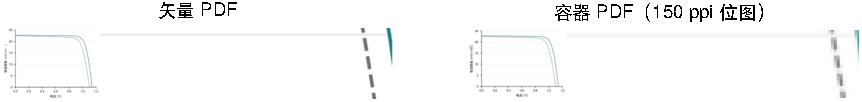
\includegraphics[width=\linewidth]{figures/ch13/ch13-05-vector-vs-container-zh.pdf}
\caption{两个都是 PDF。左：矢量对象与嵌入字体，放大后边缘锐利；右：只包着一张 150 ppi 位图，放大后出现像素格。数据为模拟数据。}\label{fig:ch13-05}
\end{figure}

\begin{table}[htbp]\centering\footnotesize
\setlength{\tabcolsep}{4pt}
\renewcommand{\arraystretch}{1.18}
\caption{对图~\ref{fig:ch13-05} 对应的两个 PDF 文件运行 \texttt{pdffonts} 与 \texttt{pdfimages -list} 的实测结果对比。}\label{tab:ch13-02}
\begin{tabularx}{\linewidth}{@{}>{\raggedright\arraybackslash}p{25mm}>{\raggedright\arraybackslash}p{22mm}Y@{}}
\toprule
\textbf{文件名与性质} & \textbf{检查命令} & \textbf{实测命令输出摘要与判读} \\
\midrule
\texttt{vector.pdf}（真矢量 PDF） & \texttt{pdffonts} & 列出 \texttt{Helvetica}（\texttt{CID TrueType}）与 \texttt{FandolHei-Regular}（\texttt{CID Type 0C}），\texttt{emb=yes}、\texttt{sub=yes}，说明中西文字体均已作为子集嵌入文件 \\
\texttt{vector.pdf}（真矢量 PDF） & \texttt{pdfimages -list} & 无任何位图条目（空白输出），证明坐标轴、网格线与两条曲线全部为纯矢量路径 \\
\texttt{container.pdf}（位图容器 PDF） & \texttt{pdffonts} & 无任何字体条目（空白输出），证明图中可见的坐标轴文字已不再是文本对象 \\
\texttt{container.pdf}（位图容器 PDF） & \texttt{pdfimages -list} & 列出第 1 页含 1 张 RGB 位图（按 150 dpi 直接封装时为 $502 \times 355\ \text{px}$、\texttt{x-ppi=150}；若经 Matplotlib \texttt{imshow} 默认 \texttt{savefig.dpi=100} 二次保存则进一步降为 $260 \times 182\ \text{px}$、\texttt{x-ppi=100}） \\
\bottomrule
\end{tabularx}
\end{table}

对照图~\ref{fig:ch13-05} 和表~\ref{tab:ch13-02}，除了可以看到左图 8 倍放大的虚线与实线边缘平滑锐利、右图 8 倍放大的曲线碎成粗糙的阶梯方格之外，这张实测图还暴露了两个在实际作图中极易踩中的隐蔽陷阱：

第一，\textbf{嵌入字体的缺字陷阱}。请仔细观察图~\ref{fig:ch13-05} 左右两张小图纵轴标题“电流密度 (\texttt{mA/cm²})”里的上标平方符号“\texttt{²}”（Unicode \texttt{U+00B2}）：因为脚本直接给整串纵轴标签指定了中文字体 \texttt{FandolHei-Regular.otf}，而该字库恰好没有收录 \texttt{U+00B2} 这个字符，结果在左边的矢量 PDF 里“\texttt{²}”直接变成了空白（显示成 \texttt{mA/cm }），而在右边的容器 PDF 里则被渲染成了一个缺字方框（俗称“豆腐块”）。这提醒我们：即便 \texttt{pdffonts} 显示 \texttt{emb=yes}，也不能省略放大肉眼核对；凡是涉及上下标（如 $\mathrm{cm^{-2}}$、$\mathrm{SnO_2}$）或特殊希腊字母（如 $\mu\mathrm{m}$）的单位，应使用数学模式（\texttt{\$\\mathrm\{mA\\,cm\^\{\{-2\}\}\}\$}）或交由字形完整的西文字体渲染。

第二，\textbf{二次封装时的静默降采样陷阱}。如表~\ref{tab:ch13-02} 最后一行所示，把一张已经按 $150\ \text{dpi}$ 渲染好的 $502 \times 354\ \text{px}$ 位图用 Matplotlib 的 \texttt{imshow} 放进新画布并调用 \texttt{savefig("container.pdf")} 时，如果忘记显式传入 \texttt{dpi} 参数，Matplotlib 会按默认的 \texttt{savefig.dpi = 100} 把画布里的位图再压缩一次，导致 PDF 内部位图进一步退化到 $260 \times 182\ \text{px}$（仅 $100\ \text{ppi}$）。只要在交付前跑一次 \texttt{pdfimages -list}，这种静默降采样一眼就能查出来。

结合前文各章，这里把 \scidraw{} 各功能模块当前导出文件的真实内部结构汇总如下，供准备终稿时核对：
\begin{itemize}
\item \textbf{科学可视化（\sdtool{sci-vis}）：}其声明式图表渲染路径导出的 PDF 与 EPS 文件属于\textbf{栅格包装容器}（内部封装的是高分辨率位图，而非可逐根拆分的矢量曲线与文字对象）。如果目标期刊强制要求数据图必须为包含嵌入字体的真矢量 PDF/EPS，作者应从 \sdtool{sci-vis} 下载校验过的数据表，用本地确定性脚本（设 \texttt{pdf.fonttype = 42}）按最终毫米尺寸输出真矢量 PDF。
\item \textbf{图像转 SVG 与图像转 PPTX：}把位图转成 SVG 时，即便选用“文字层模式”，生成的 SVG 底部仍然包含一张位图背景；转成 PPTX 时，得到的是“一张去字背景位图 + 经光学字符识别（OCR）生成的独立文本框”，并不会把画面里的细胞、晶粒或曲线自动变成带有科研语义的矢量图形。
\item \textbf{组图工具（\sdtool{multi-panel-figure-maker}）：}导出的 PPTX 文件中，各个子面板是独立位图，左上角的面板编号（\textbf{a}、\textbf{b}、\textbf{c}、\textbf{d}）是可编辑文本框，面板内部的曲线和标签则不能在 PowerPoint 里逐条拆开编辑。
\end{itemize}

\section{颜色：RGB/CMYK、灰度与色觉差异}

颜色检查要解决三个问题：文件该存什么色彩空间？打印成黑白灰阶后各组还能不能分清？对存在色觉差异的同行读者是否友好？

\subsection*{RGB 与 CMYK：保留 RGB 母版，不要盲目自行转 CMYK}

屏幕显示器靠红、绿、蓝三原色光叠加显色（RGB 加色模式，色域较宽），而纸质印刷机靠青、品红、黄、黑四色油墨叠印显色（CMYK 减色模式，色域较窄，尤其难以印出屏幕上那种高饱和度的亮绿、亮青和荧光蓝）。

早期许多作图教程会笼统建议作者“投稿前把所有图片转成 CMYK”，但这一建议早已不符合当今主流科学期刊的出版流程。如今绝大多数学术阅读发生在线上 HTML 与 PDF 版本中；查阅本章核对的三家代表性出版社官方页面（截至 2026 年 10 月 29 日），可以看到它们一致推荐或优先接受 RGB：
\begin{itemize}
\item \textbf{Nature：}明确建议作者提交 RGB 图像；期刊生产系统会在纸质印刷时自动将 RGB 转为 CMYK，同时在网络版与在线 PDF 中完整保留色彩更丰富的 RGB 原图。
\item \textbf{Elsevier：}在图件说明中写明“RGB 优先（RGB preferred）”。
\item \textbf{PLOS ONE：}作为纯在线开放获取期刊，只要求提交每通道 8 位的 RGB（或灰度）图像。
\end{itemize}

如果作者在本地用不明来源的通用印刷配置文件（ICC profile）自行把图片转成了 CMYK，不仅在线读者看到的颜色会变得暗淡发闷，一旦所选油墨配置与印厂实际设备不匹配，还会造成二次偏色。因此，正确做法是：\textbf{始终保留嵌入标准 sRGB 配置文件的 RGB 母版并优先提交 RGB；只有当目标期刊的现行作者指南明确要求提交 CMYK 文件时，才在副本上转换，并在转换后逐一核对高饱和色块是否发生了明显的色相偏移或层次并拢。}

\subsection*{灰度可读性：用感知明度 $L^*$ 检查，而不是三通道求平均}

合作者拿着黑白打印稿问小周“哪条是对照”，戳中的正是我们在第 9 章和第 12 章留下的一处真实隐患。

第 12 章在设计钙钛矿研究配色时，为了避开刺眼的红绿撞色，选用了沉稳的深灰（\texttt{\#6E6E6E}，对照组）配青色（\texttt{\#1B7F86}，改性组）。在彩色屏幕上，这两种颜色一个偏中性灰、一个偏蓝绿，感知色差（CAM02-UCS $\Delta E$）达到 $19.8$，看起来区分度相当不错。然而，当打印机或阅读器把彩色转成灰度时，人眼感受到的明暗并不是简单地把十进制 RGB 三通道加起来除以 3，而是由符合人眼光谱灵敏度的\textbf{相对亮度（luminance $Y$）与 CIE 1976 感知明度 $L^*$} 决定的。

在标准 sRGB 色彩空间中，需先将经过伽马编码的通道值还原为线性光强 $C_{\text{lin}}$，再按 Rec.~709 权重计算相对亮度：
\[
Y = 0.2126\,R_{\text{lin}} + 0.7152\,G_{\text{lin}} + 0.0722\,B_{\text{lin}}
\]
接着将 $Y$ 非线性映射为范围在 $0\text{--}100$ 之间的感知明度 $L^*$。注意到绿色通道的权重高达 $0.7152$，红色为 $0.2126$，蓝色只有 $0.0722$。我们用这套标准公式算一下本章案例与常见草稿里的四个颜色：
\begin{itemize}
\item 对照组深灰 \texttt{\#6E6E6E}（$\text{RGB} = 110, 110, 110$）：感知明度 $\mathbf{L^* = 46.4}$；
\item 改性组青色 \texttt{\#1B7F86}（$\text{RGB} = 27, 127, 134$）：虽然蓝绿醒目，但红光分量极低，折算下来感知明度 $\mathbf{L^* = 48.4}$；
\item 常见草稿红 \texttt{\#CC0000}（$\text{RGB} = 204, 0, 0$）：感知明度 $L^* = 42.5$；
\item 常见草稿绿 \texttt{\#2CA02C}（$\text{RGB} = 44, 160, 44$）：感知明度 $L^* = 57.9$。
\end{itemize}

算式直接揭示了真相：\textbf{对照组深灰（$L^* = 46.4$）与改性组青色（$L^* = 48.4$）的感知明度只差 $2.0$ 个单位，灰度下的色差 $\Delta E$ 跌到了 $2.1$！}当两条同样粗细的实线以 $L^* = 46.4$ 和 $48.4$ 印在白纸上时，任何人的肉眼都无法分辨哪条是灰、哪条是青。这就是为什么灰度检查绝不能只靠“看着颜色不一样”来拍脑袋，必须做一次真实的 $L^*$ 灰度转换。

\subsection*{色觉差异模拟与双重编码}

除了黑白打印，科研图还直接面对具有色觉差异（colour-vision deficiency, CVD）的审稿人与读者。人类视网膜包含对长波（L，偏红）、中波（M，偏绿）和短波（S，偏蓝）敏感的三类视锥细胞。根据受影响的视锥细胞类型，先天性色觉差异主要分为三类：
\begin{enumerate}
\item \textbf{红色觉异常（protan，L 视锥异常）：}包括红色弱（protanomaly）与红色盲（protanopia），对长波红光敏感度降低，不仅红绿难辨，而且纯红色在视觉上会明显变暗。
\item \textbf{绿色觉异常（deutan，M 视锥异常）：}包括绿色弱（deuteranomaly）与绿色盲（deuteranopia），是最常见的一类，红与绿在视觉上都会坍缩成相似的黄褐色或橄榄色。
\item \textbf{蓝色觉异常（tritan，S 视锥异常）：}包括蓝色弱（tritanomaly）与蓝色盲（tritanopia），较为少见，主要表现为蓝与绿、黄与紫之间的混淆。
\end{enumerate}

正如 Wong（2011）在关于科研配色的专栏中所指出的，在北欧血统人群中，通常估计约有 $8\%$ 的男性（以及约 $0.5\%$ 的女性）存在某种程度的红绿色觉差异。此外，Crameri 等人（2020）系统论证了传统彩虹色图（如 Jet）不仅会让色觉差异读者无法分辨红绿两端，还会因为本身明度梯度不均匀而在连续数据中制造出虚假的边界与伪影。

要在作图阶段检验配色在色觉差异下的表现，科学界常用基于视觉生理模型的计算机模拟算法。早期广泛使用的方法是 Brettel 等人（1997）针对完全二色视提出的 LMS 色彩空间投影模型；后来 Machado、Oliveira 与 Fernandes（2009）提出了一套基于视锥色素光谱位移理论的生理模型，将色觉异常从轻微异常三色视到完全二色视统一参数化为严重度 $0\text{--}100$，并给出了直接作用于\textbf{线性 RGB 空间}的 $3 \times 3$ 转换矩阵。

图~\ref{fig:ch13-06} 采用 Python 的 \texttt{colorspacious} 库（1.1.2 版，经核对其内部矩阵与 Machado 等人 2009 年补充材料数值一致），在最高严重度（\texttt{severity = 100}，近似完全二色视）下，对比了钙钛矿稳定性曲线三种配色方案在原图、CIE $L^*$ 灰度以及红色弱（protan）、绿色弱（deutan）、蓝色弱（tritan）五种视图下的表现，并在每个子图右上角标出了两条曲线在当前视图下的 CAM02-UCS 色差 $\Delta E$。

\begin{figure}[htbp]\centering
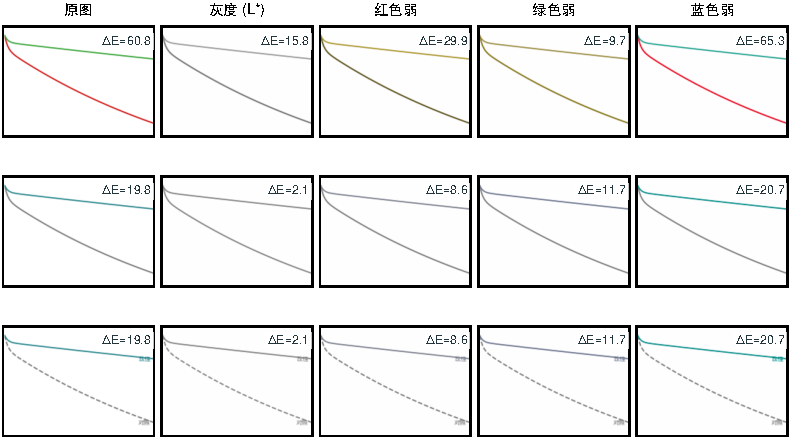
\includegraphics[width=\linewidth]{figures/ch13/ch13-06-grayscale-and-cvd-zh.pdf}
\caption{同一张图的三种配色在灰度与色觉差异模拟下的表现。第 2 行（第 12 章配色）在灰度下两组几乎无法区分；第 3 行改用线型后，在所有视图中都能区分。色觉模拟采用 Machado 等（2009）的模型，严重度 100，仅为近似。数据为模拟数据。}\label{fig:ch13-06}
\end{figure}

我们逐行核对图~\ref{fig:ch13-06} 的实测结果：
\begin{itemize}
\item \textbf{第 1 行（红 \texttt{\#CC0000} 与绿 \texttt{\#2CA02C} 实线草稿）：}在原图（$\Delta E = 60.8$）和蓝色弱（$\Delta E = 65.3$）下反差强烈；在灰度下因该红与该绿恰好有明度差（$L^*$ 分别为 $42.5$ 与 $57.9$），仍保留了 $\Delta E = 15.8$ 的深浅区别；但在最常见的绿色弱模拟（第 4 列）下，两条曲线双双变成了暗黄褐色，$\Delta E$ 骤降到 $9.7$，一旦加上图例框让读者跨空间比对颜色，极易认反。
\item \textbf{第 2 行（第 12 章初始配色：对照灰 \texttt{\#6E6E6E} 与改性青 \texttt{\#1B7F86} 均为实线）：}在红色弱（$\Delta E = 8.6$）、绿色弱（$\Delta E = 11.7$）和蓝色弱（$\Delta E = 20.7$）下尚能保持色调差异；然而一进入第 2 列的灰度（$L^*$）视图，$\Delta E$ 直接坍缩到 $\mathbf{2.1}$，上下两条实线变成了几乎完全相同的中灰色，复现了合作者拿着黑白打印稿分不清哪条是对照的场景。
\item \textbf{第 3 行（修正版：保留灰青颜色，对照组改为虚线、改性组保持实线，并在曲线右端直接标注“改性”“对照”）：}请注意，第 3 行右上角的五个颜色 $\Delta E$ 数值（$19.8$、$2.1$、$8.6$、$11.7$、$20.7$）与第 2 行分毫不差，因为我们根本没有改动两种颜色的色值；但是，由于引入了\textbf{线型（虚线对实线）}和\textbf{曲线末端直接文字标注}，即便在灰度 $\Delta E = 2.1$ 的极端情况下，任何读者也能在一秒钟内准确分清上下两条曲线。
\end{itemize}

同时，观察图~\ref{fig:ch13-06} 第 3 行的缩略图还能看到一个值得留意的细节：由于小网格缩略图里直接把 $5\ \text{pt}$ 的“改性”“对照”两个标签以垂直居中方式写在了 $t = 980\ \text{h}$ 的曲线末端坐标上，曲线本身从文字正中间穿了过去。因此，在正式制作论文终稿（如第 9 章终稿与本章交付版）时，应当把直接标注向曲线上方、下方或左侧空白处微调偏移，避免线条横穿文字笔画。

在使用任何色觉差异模拟时，必须清楚它的两条局限：第一，模拟只是针对特定理论参数的数学近似，真实个体的视锥光谱偏移程度与显示器状态各不相同，模拟通过并不等于拿到了某种绝对的“色盲无障碍认证”；第二，正如 Machado 等人（2009）在原论文中讨论的，受限于人类蓝色觉异常（tritan）的经验心理物理学数据较少，tritan 模拟矩阵的可靠性低于 protan 和 deutan。正因为如此，最稳妥的做法永远不是赌某两个颜色在所有人的眼睛里都能拉开差距，而是贯彻\textbf{双重编码（redundant encoding）}：凡是承载核心分组对比的元素，在颜色之外永远同时配上不同的线型、散点形状或直接文字标注。

\section{用 \sdtool{figure-checker} 做技术检查}

完成上述手动换算后，可以借助 \scidraw{} 的图片检查工具（即 \sdtool{figure-checker}）把与位图文件相关的技术指标做一次自动化筛查。

打开该工具上传 PNG、JPEG、WebP 或 TIFF 格式的图像后，在“图类型”中按内容选择\textbf{照片}、\textbf{混合图}或\textbf{线条图}，并在“目标版面”中选择预设的单栏（$85\ \text{mm}$）、双栏（$180\ \text{mm}$）或切换到\textbf{自定义宽度}输入精确毫米数。工具会输出六项技术检查结果与预览：(1) \textbf{有效分辨率}（按目标宽度换算；照片 $\ge 300\ \text{ppi}$、混合 $\ge 600\ \text{ppi}$、线条图 $\ge 900\ \text{ppi}$ 为“通过”，低一档为“提醒”）；(2) \textbf{文件格式}；(3) \textbf{Alpha 透明通道}（提醒去除透明背景以免排版变黑块）；(4) \textbf{色彩空间}；(5) \textbf{灰度亮度层级数与灰度预览}；(6) \textbf{三类色觉模拟下主要颜色簇是否塌缩及色觉预览}。

将报告收入交付包时，作者必须牢记五条边界——\textbf{切勿把工具界面上的“通过”当成“符合期刊全部投稿要求”}：
\begin{enumerate}
\item \textbf{它是技术检查，不是科学审核：}工具不检查统计方法、误差线定义、数据真实性或期刊特定的政策要求。
\item \textbf{默认双栏（$180\ \text{mm}$）不等于具体期刊的实际栏宽：}Nature 双栏为 $183\ \text{mm}$、Cell/Springer 为 $174\ \text{mm}$、Elsevier 为 $190\ \text{mm}$，而组图中的单个半栏面板往往只有 $84\ \text{mm}$ 或 $92\ \text{mm}$ 宽。因此检查时应改用\textbf{自定义宽度}填入真实毫米数。
\item \textbf{它不检查字号、线宽与 PDF 内部矢量结构：}一张把文字缩到 $4.5\ \text{pt}$ 的图，只要存成 $600\ \text{dpi}$ PNG，在分辨率项上照样会显示“通过”。字号与线宽须按第 13.2 节核对，PDF 内部结构须按第 13.3 节用 \texttt{pdffonts} 和 \texttt{pdfimages -list} 核对。
\item \textbf{工具内置阈值不等同于具体期刊标准：}例如工具对线条图设 $\ge 900\ \text{ppi}$ 为通过，而 Elsevier 官方指南要求线条图位图至少 $1000\ \text{dpi}$（细线 $1200\ \text{dpi}$），投稿时一律以目标期刊指南为准。
\item \textbf{自动灰度与色觉判据不能替代肉眼审视预览图：}全局灰度层级统计包含黑轴、网格和白底，未必会针对图中央两条明度相近的数据线单独报警，且快速色觉预览算法与本书图~\ref{fig:ch13-06} 采用的 Machado 矩阵结果可能略有差别，最终结论应以“点开预览图看各组是否靠线型、形状或明度清晰可分”为准。
\end{enumerate}

\section{期刊要求：以当前官方页面为准}

表~\ref{tab:ch13-01} 汇总了我们在 **2026 年 10 月 29 日** 直接打开并核对的三家出版社/期刊官方图件指南页面要点：Nature（\textit{Guide to preparing final artwork}）、PLOS ONE（\textit{Figures}）以及 Elsevier（\textit{Artwork sizing} 与 \textit{Artwork types}）。

\begin{table}[htbp]\centering\footnotesize
\setlength{\tabcolsep}{3pt}
\renewcommand{\arraystretch}{1.18}
\caption{三家期刊/出版社官方图件技术要求核对表（查阅日期：2026 年 10 月 29 日；投稿前请重新查阅目标期刊当前官方页面）。}\label{tab:ch13-01}
\begin{tabularx}{\linewidth}{@{}>{\raggedright\arraybackslash}p{18mm}YYY@{}}
\toprule
\textbf{事项} & \textbf{Nature（\textit{Guide to preparing final artwork}）} & \textbf{PLOS ONE（\textit{Figures}）} & \textbf{Elsevier（\textit{Artwork sizing / types}）} \\
\midrule
版面宽度 & 单栏 $89\ \text{mm}$；双栏 $183\ \text{mm}$；1.5 栏 $120$ 或 $136\ \text{mm}$ & 宽 $6.68\text{--}19.05\ \text{cm}$（$300\ \text{dpi}$ 下 $789\text{--}2250\ \text{px}$） & 最小 $30\ \text{mm}$；单栏 $90\ \text{mm}$；1.5 栏 $140\ \text{mm}$；双栏 $190\ \text{mm}$ \\
最大高度 & $247\ \text{mm}$ & $22.23\ \text{cm}$（$300\ \text{dpi}$ 下 $2625\ \text{px}$） & 该页面未单独列出固定最大高度 \\
分辨率要求 & 照片按印刷最大尺寸 $\ge 300\ \text{dpi}$；线条图与文字不要栅格化 & $300\text{--}600\ \text{dpi}$ & 照片 $300\ \text{dpi}$；组合图 $500\ \text{dpi}$；线条图 $1000\ \text{dpi}$（细线 $1200\ \text{dpi}$） \\
可接受格式 & AI、矢量 EPS、分层 PSD、PS、PDF、PPT、Word、Excel、CorelDraw（$\le\text{v8}$）；JPEG/TIFF/PNG 须转为 PDF/EPS/PS & TIFF 或 EPS & 线条图 EPS 或 TIFF；照片/组合图 TIFF 或最高质量 JPEG；Office 文件按混合矢量处理 \\
色彩空间 & 推荐 RGB；印刷时自动转 CMYK，在线 PDF 保留 RGB & RGB（每通道 8 bit）或灰度 & RGB 优先（RGB preferred） \\
字体与字号 & 无衬线（Helvetica 或 Arial）；面板字母 $8\ \text{pt}$ 粗体小写；其余文字最大 $7\ \text{pt}$、最小 $5\ \text{pt}$；不要转曲 & Arial、Times 或 Symbol，字号 $8\text{--}12\ \text{pt}$ & 必须嵌入字体；首选 Arial/Helvetica、Courier、Times、Symbol；正文最终 $7\ \text{pt}$，上下标 $\ge 6\ \text{pt}$ \\
其他规定 & — & 单文件 $< 10\ \text{MB}$；TIFF 去图层、无 Alpha、LZW 压缩；推荐 NAAS 预检 & 线宽保持在 $0.10\text{--}1.5\ \text{pt}$ 之间 \\
\bottomrule
\end{tabularx}
\end{table}

对比表~\ref{tab:ch13-01} 中的具体条款，有三个事实必须写进任务书：
\begin{enumerate}
\item \textbf{不同期刊的硬指标可能互相冲突：}例如 Nature 要求除面板编号（$8\ \text{pt}$）外的普通标签文字\textbf{最大不超过 $7\ \text{pt}$}（$5\text{--}7\ \text{pt}$），而 PLOS ONE 则要求图内文字在 \textbf{$8\text{--}12\ \text{pt}$} 之间。若论文换期刊重投，必须在脚本里改字号参数重新出图。
\item \textbf{同一出版社内部的不同官方指南也可能存在细微出入：}例如表~\ref{tab:ch13-01} 引用的 Nature 终稿指南规定单栏 $89\ \text{mm}$、双栏 $183\ \text{mm}$，而 Nature 旗下另一份通用图件指南文件则写着单栏 $88\ \text{mm}$、双栏 $180\ \text{mm}$，相差 $1\text{--}3\ \text{mm}$。\scidraw{} 组图工具内置期刊尺寸预设时专门记录了所依据的官方页面；投稿前仍应打开所投具体期刊当年的作者指南页复核。
\item \textbf{必须把“官方页面 URL 与查阅日期”写进任务书和交付说明：}你可以请 AI 助手帮你从指南网页摘录要点，但摘录后必须回到官方原网页逐个数字核对，并在任务书中写明查阅日期。
\end{enumerate}

\section{整理一个可追溯的交付包}

当所有图片都通过核验后，最后一步是把散落的材料整理成一个\textbf{同事无需找你问话就能独立看懂、定位和复现的交付包}。遵循科学数据管理的 FAIR 原则（Wilkinson 等，2016）与可复现计算研究十条规则（Sandve 等，2013），图~\ref{fig:ch13-08} 给出了可直接照抄的课题组级交付包标准目录树。

\begin{figure}[htbp]\centering
{\let\tag\undefined\makeatletter\tikzset{below/.code=\tikz@lib@place@handle@{#1}{north west}{0}{-1}{south west}{1}}\makeatother% FIG ch13-08 delivery package tree (Chinese)
\usetikzlibrary{positioning}
\providecommand{\ChThirteenMarkTool}{\tikz[baseline=-0.55ex]{\fill[BookInk] (0,0) rectangle (1.5mm,1.5mm);}}
\providecommand{\ChThirteenMarkSelf}{\tikz[baseline=-0.55ex]{\draw[BookInk, line width=0.35pt] (0,0) rectangle (1.5mm,1.5mm);}}
\providecommand{\tag}[1]{{\tiny\color{BookInk!75}#1}}
\noindent
\begin{tikzpicture}[
  font=\sffamily\scriptsize, text=BookInk,
  folder/.style={anchor=west, align=left},
  tagline/.style={font=\tiny, text=BookInk!75, align=left},
]
  \node[folder] (root) at (0,0) {perovskite-fig2\_\\delivery\_2026-10-29/};
  \node[folder, below=2mm of root.south west, xshift=4mm] (readme) {README.md};
  \node[tagline, below=0.5mm of readme.south west] (readmetag) {这是什么、\\怎么复现、\\联系人};
  \node[folder, below=1.5mm of readmetag.south west, xshift=4mm] (b0) {00\_brief/\\[-2pt]\tag{任务书、}\\[-1pt]\tag{期刊要求摘录}};
  \node[folder, below=1.5mm of b0.south west, xshift=4mm] (s1) {01\_source/ \ChThirteenMarkSelf\ 原图与 CSV\\[-2pt]\tag{工具 ZIP 不含}};
  \node[folder, below=1.5mm of s1.south west, xshift=4mm] (s1d) {data/ · images/};
  \node[folder, below=1.5mm of s1d.south west] (c2) {02\_code/ \ChThirteenMarkSelf\ 脚本与环境};
  \node[folder, below=1.5mm of c2.south west, xshift=4mm] (d3) {03\_drafts/ \ChThirteenMarkSelf\ v01–v04\\[-2pt]与修改指令};
  \node[folder, below=1.5mm of d3.south west, xshift=4mm] (f4) {04\_final/ \ChThirteenMarkTool\ 论文/汇报/\\[-2pt]海报终稿};
  \node[folder, below=1.5mm of f4.south west, xshift=4mm] (f4p) {paper/ · talk/ · poster/};
  \node[folder, below=1.5mm of f4p.south west] (r5) {05\_records/};
  \node[folder, below=1.5mm of r5.south west, xshift=4mm] (r5a) {ai-use-log.md \ChThirteenMarkSelf};
  \node[folder, below=1mm of r5a.south west] (r5b) {processing-log.md \ChThirteenMarkSelf};
  \node[folder, below=1mm of r5b.south west] (r5c) {checks/ \ChThirteenMarkTool\ 检查报告\\[-2pt]与命令输出};
  \node[folder, below=1mm of r5c.south west] (r5d) {multi-panel-export/ \ChThirteenMarkTool\ 组图 ZIP};

  \draw[BookInk!40, thin] (root.south west) ++(0,-1mm) coordinate (rt) -- (readme.west |- rt) -- (readme.west);
  \foreach \a/\b in {readmetag/b0,b0/s1,s1/s1d,s1d/c2,c2/d3,d3/f4,f4/f4p,f4p/r5,r5/r5a,r5a/r5b,r5b/r5c,r5c/r5d} {
    \draw[BookInk!30, thin] (\a.south west) ++(0,-0.5mm) coordinate (st) -- (\b.west |- st) -- (\b.west);
  }

  \node[tagline, anchor=north west] at ([yshift=-3mm]r5d.south-|root.west) {%
    \ChThirteenMarkTool\ 来自工具导出（组图 ZIP、\\数据下载、检查报告）\\[2pt]
    \ChThirteenMarkSelf\ 必须作者另存（原图、脚本、\\任务书、AI 使用记录）\\[4pt]
    README 三问：这是什么？\\怎么复现？\\用了哪些 AI、怎么核对的？};
\end{tikzpicture}
}
\caption{一个可被同事接手的交付包。黑色方块表示可由工具导出的内容，空心方块表示需要作者另存的材料。}\label{fig:ch13-08}
\end{figure}

图~\ref{fig:ch13-08} 用实心方块与空心方块区分了“可由工具导出的内容”和“必须由作者另存的材料”。之所以要做这个区分，是因为作者必须清楚了解当前平台上各工具的本地存储与导出边界：
\begin{itemize}
\item \textbf{组图 ZIP 不含原图与可重载工程：}组图工具导出的 ZIP 压缩包内含合成终稿（TIFF、PNG、PDF、PPTX）及处理记录（\texttt{processing-log}），但\textbf{不含未裁剪缩放的面板原始文件，也不含可跨电脑重新导入的布局文件}；组图文档只保存在当前浏览器的本地存储中，换电脑无法打开，因此 \texttt{01\_source/} 必须另存原图，\texttt{04\_final/} 保存导出成品。
\item \textbf{数据图记录源数据完整性但脚本需自存：}\sdtool{sci-vis} 会自动记录上传源数据的完整性信息（哈希值、字节数、行数）并提供数据表下载，但底层绘图代码不作为当前读者端可下载内容，因此复现脚本应保存在 \texttt{02\_code/}。
\end{itemize}

为了告别混乱命名，包内所有文件统一采用四段式命名规则：\texttt{<项目>\_<图号或用途>\_<内容>\_v<两位版本>[\_<语言>].<扩展名>}（如 \texttt{perovskite\_fig2c\_jv\_v05\_en.pdf}、\texttt{perovskite\_\allowbreak slide2b\_\allowbreak jv\_\allowbreak v02\_\allowbreak zh.png}）。执行时遵守三条纪律：(1) 只用小写 ASCII 字母、数字、连字符和下划线，不用空格或中文符号；(2) 版本号只增不改（\texttt{v01}、\texttt{v02}……），禁用 \texttt{final\_final}，日期写在交付包目录名和日志里；(3) 哪一版是“已投稿版本”在根目录 \texttt{README.md} 中唯一指明。

在 \texttt{05\_records/} 目录中，核心文档是 \textbf{AI 使用记录（\texttt{ai-use-log.md}）}与\textbf{处理记录（\texttt{processing-log.md}）}。可直接复制的 AI 使用记录模板如下：

\begin{Prompt}
# AI 使用记录 / AI-use log
项目：perovskite-passivation   图号/用途：Figure 2 / 汇报 / 海报   记录人：小周
| 日期 | 工具与功能 | 输入（版本/行数/哈希） | 实际提示词或指令路径 | 输出文件（版本） | 是否采用 | 人工核对与修改 |
|---|---|---|---|---|---|---|
| 2026-10-29 | /ai-drawing | 任务书 v1（面板 a） | 03_drafts/v01/m1_prompt.txt | m1_base_v02.png | 采用底图 | 核对 7 层顺序无误；后期叠加 7 pt 矢量层名 |
| 2026-10-29 | /ai-drawing | 任务书 v1（面板 b） | 03_drafts/v01/m2_prompt.txt | m2_sem_v01.png | 采用底图 | 确认无伪比例尺；图内左下角加“模型生成示意” |
| 2026-10-29 | /sci-vis | metrics.csv（2 行） | 03_drafts/v04/jv_instr.txt | fig2c_jv_v04.png | 部分采用 | 核对 PCE 一致；改用脚本重绘真矢量 PDF（v05） |
## 不使用 AI 的环节
数据模拟与指标计算由 02_code/sim_perovskite.py 完成；图注中的实验与模拟条件由作者撰写。
## 生成图像的证据状态
M1 为结构示意（标“不按比例”）；M2 为模型生成截面示意，非显微图像（在所有版本图内标注）。
## 期刊 AI 政策
查阅政策 URL 与日期：Elsevier AI author policy (2026-10-29)   是否需声明：按期刊要求填写。
\end{Prompt}

配套的 \texttt{processing-log.md} 则专门记录确定性处理参数：数据模拟参数与脚本版本、是否经过筛选或变换（本例无）；图像 \texttt{M1}、\texttt{M2} 的生成输入与后期缩放裁剪比例（如 \texttt{M2} 仅等比缩放、无局部修改，可直接引用组图处理记录）；以及因 P3 灰度问题修改线型的原因。

\section{完整案例：交付钙钛矿研究 Figure 2 及其衍生版本}

现在我们跟着小周把论文 Figure 2（投往执行 Elsevier 通用图件要求的期刊）、3 页组会汇报与 A0 海报走完交付全流程。

\textbf{第一步：编写交付任务书}（保存为 \texttt{00\_brief/delivery-brief.txt}）。

\begin{Prompt}
【交付对象】论文 Figure 2（四面板）；汇报第 1–3 页；A0 海报。
【目标期刊要求，查阅日期 2026-10-29】Elsevier artwork sizing / artwork types 页面：
  双栏 190 mm；正文字最终 7 pt，上下标不小于 6 pt；线宽 0.10–1.5 pt；
  线条图位图 >= 1000 dpi，组合图 >= 500 dpi，照片 >= 300 dpi；RGB 优先；嵌入字体。
【面板性质】a 示意（位图底图 + 矢量文字）；b 模型生成示意（位图）；c、d 数据图（应为真矢量）。
【检查项】有效分辨率；最终字号与线宽；c、d 为真矢量且字体嵌入；灰度与三类色觉模拟下两组可区分；图内证据标注齐全。
【不可改变】数据点（对照 PCE 19.21%、T80 约 210 h；改性 PCE 20.98%、1000 h 保留约 86%）、坐标范围、两组含义。
【交付与验收】按图 13-8 目录归档；同事只看 README 能在 10 分钟内找到 Figure 2c 的原始 CSV、生成脚本与修改指令。
\end{Prompt}

\textbf{第二步：第一轮检查结果（\texttt{v04} 初稿）。}小周对第 4 版初稿（\texttt{v04}）运行命令行检查、字号换算、CIE $L^*$ 灰度计算与 \sdtool{figure-checker} 后，发现了表~\ref{tab:ch13-case-round1} 所示的四项问题（P1–P4）。

\begin{table}[htbp]\centering\footnotesize
\setlength{\tabcolsep}{3pt}
\renewcommand{\arraystretch}{1.18}
\caption{钙钛矿研究 Figure 2 及衍生版本的第一轮交付检查结果（v04 初稿）。}\label{tab:ch13-case-round1}
\begin{tabularx}{\linewidth}{@{}c>{\raggedright\arraybackslash}p{22mm}>{\raggedright\arraybackslash}p{26mm}Y>{\raggedright\arraybackslash}p{16mm}@{}}
\toprule
\textbf{编号} & \textbf{检查项目} & \textbf{检查方法} & \textbf{实测结果与诊断} & \textbf{严重度} \\
\midrule
P1 & c、d 导出文件是否矢量 & 对从 \sdtool{sci-vis} 下载的 PDF 跑 \texttt{pdffonts}、\texttt{pdfimages -list} & 无字体条目、内含 1 张位图，属于栅格包装容器 & 高 \\
P2 & a 面板标签字号 & 把 a 源图（按 $7.3\ \text{in}$ 宽、$10\ \text{pt}$ 作图）缩进 $190\ \text{mm}$ 双栏的半栏（约 $92\ \text{mm}$） & $10 \times 92 \div 185.4 \approx 5.0\ \text{pt}$，低于 Elsevier 要求的 $7\ \text{pt}$ & 高 \\
P3 & 灰度可区分性 & 计算 CIE $L^*$：对照 \texttt{\#6E6E6E} $= 46.4$，改性 \texttt{\#1B7F86} $= 48.4$ & 两条实线在灰度下 $\Delta E = 2.1$，黑白打印几乎无法区分 & 中 \\
P4 & 位图有效分辨率 & b 面板（$1536 \times 1024\ \text{px}$）放 $92\ \text{mm}$ 宽（或 $174\ \text{mm}$ 版式的 $69\ \text{mm}$ 宽） & $1536 \div (92 \div 25.4) \approx 424\ \text{ppi}$（$69\ \text{mm}$ 时 $565\ \text{ppi}$）；a 底图（$1586 \times 992\ \text{px}$）在 $92\ \text{mm}$ 时为 $438\ \text{ppi}$。按照片类 $\ge 300\ \text{dpi}$ 满足，记录于交付说明 & 低 \\
P5 & 证据标注 & 逐图查看论文、汇报、海报 & 汇报第 2、3 页和海报均有“模拟数据”；论文 b、汇报备用页和海报均有“模型生成示意，非显微图像” & 通过 \\
\bottomrule
\end{tabularx}
\end{table}

\textbf{第三步：开具修改指令（\texttt{v04} $\rightarrow$ \texttt{v05}）。}

针对 \textbf{P1}，若在 \sdtool{sci-vis} 历史会话中确认导出格式，可输入：
\begin{Prompt}
保持数据、坐标范围、颜色和全部标注不变。我需要可编辑矢量版本用于期刊排版：
请说明当前可以导出的格式中，哪些包含矢量路径和可编辑文字。
\end{Prompt}
确认声明式路径导出的 PDF 为栅格容器后，小周改用 \texttt{02\_code/} 中的 Matplotlib 脚本读取同一份 CSV 数据（设 \texttt{pdf.fonttype = 42}）按最终物理尺寸重绘真矢量 PDF，并在处理记录中写明：“c、d 面板由脚本重绘以获得矢量文件；数值与 \sdtool{sci-vis} 版本及 \texttt{metrics.csv} 逐点核对一致。”

针对 \textbf{P2}（重绘 a 面板标签，不重新生成底图）：
\begin{Prompt}
保留 a 面板底图（v04）不变。在矢量叠加层中把所有层名改为 7 pt（最终 92 mm 宽时），
字体 Arial/Helvetica（或 TeX Gyre Heros），嵌入字体；标签与层的对应关系不变。
\end{Prompt}

针对 \textbf{P3}（数据图配色与线型双重编码）：
\begin{Prompt}
保持全部数据点、坐标、标注文字不变。对照组改为虚线（线宽 1.0 pt，颜色 #6E6E6E），
改性组保持实线 #1B7F86（1.0 pt）。面板 d 的 80% 参考线改为细点线。保留曲线末端的直接标注并避开线条。
\end{Prompt}
这一灰度问题正是在本章交付检查计算 CIE $L^*$ 时才被发现的。发现后，我们将“对照虚线、改性实线、80\% 参考线点线”回写到了第 9 章与第 12 章的终稿中，从而保证全书各章终稿与交付包中的 \texttt{v05} 版本完全一致。

\textbf{第四步：第二轮复查、终稿图注与交接验收。}复查修订后的 \texttt{v05} 确认：论文版 PDF 的 \texttt{pdffonts} 显示全部字体已嵌入，\texttt{pdfimages -list} 仅含 a、b 两张底图位图（若投稿系统要求位图 TIFF，则按线条图 $1000\ \text{dpi}$ 要求导出 $190\ \text{mm} \rightarrow 7480\ \text{px}$ 宽的 LZW 压缩 RGB TIFF）；汇报幻灯片 PNG 为 $1920 \times 1080\ \text{px}$；海报 A0 PDF 字体全部嵌入，\texttt{pdfimages -list} 仅列出 M1（$2129 \times 1332\ \text{px}$、$150\ \text{ppi}$）与 M2（$1063 \times 709\ \text{px}$、$150\ \text{ppi}$）两张位图。更新后的论文图注终稿如下：

\begin{BookNote}
\textbf{图 2}\quad 界面钝化对模拟器件性能与稳定性的影响（模拟教学数据）。(a) n-i-p 器件结构示意，不按比例。(b) 截面图样，为模型生成示意，非显微图像。(c) 模拟反向扫描 J–V 曲线（单二极管模型，AM1.5G，$100\ \text{mW\,cm}^{-2}$），对照为虚线、改性为实线；每组一条代表性曲线。(d) 归一化 PCE 随时间变化（模拟），细点线为初始值的 80\%（参考线用点线，以免与对照组的虚线混淆）。\\[3pt]
\textbf{Figure 2}\quad Effect of interfacial passivation on simulated device performance and stability (simulated teaching data). (a) Schematic of the n-i-p stack, not to scale. (b) Cross-section, model-generated illustration, not a micrograph. (c) Simulated reverse-scan J–V curves (single-diode model, AM1.5G, $100\ \text{mW\,cm}^{-2}$); control dashed, modified solid; one representative curve per group. (d) Normalized PCE over time (simulated); the thin dotted line marks 80\% of the initial value.
\end{BookNote}

最后，未参与作图的师妹仅阅读根目录下的 \texttt{README.md}，在 6 分钟内顺利找到原始数据表（\texttt{01\_source/data/}）、模拟与绘图脚本（\texttt{02\_code/}）以及第 4 版修改指令（\texttt{03\_drafts/v04/}），重跑脚本验证两组 PCE（$19.21\%$ 与 $20.98\%$）与指标表完全一致，顺利完成交接验收。

\section{AI 在这一步能做什么与不能做什么}

印前检查、格式导出与交付环节中 AI 与作者的职责边界汇总于表~\ref{tab:ch13-03}。

\begin{table}[htbp]\centering\footnotesize
\setlength{\tabcolsep}{3pt}
\renewcommand{\arraystretch}{1.18}
\caption{检查、导出与交付环节中 AI 能做什么、不能做什么与作者必须核对的内容。}\label{tab:ch13-03}
\begin{tabularx}{\linewidth}{@{}>{\raggedright\arraybackslash}p{18mm}YYY@{}}
\toprule
\textbf{环节} & \textbf{AI 能做} & \textbf{AI 不能做} & \textbf{作者要核对} \\
\midrule
尺寸与分辨率 & \sdtool{figure-checker} 按目标宽度换算有效分辨率；组图导出按真实尺寸换算 & 用放大“补回”原始图像缺失的信息；替你决定图该放单栏还是双栏 & 像素 $\div$ 最终宽度的算式；证据图像不经 AI 放大 \\
字号与线宽 & 按指令重绘数据图、调整字号 & 保证最终版面中的实际字号；知道排版时会被缩放多少 & 按最终宽度作图；100\% 样张实测 \\
文件格式 & 导出多种格式；把位图转成 SVG/PPTX 以便编辑 & 保证导出的 PDF/SVG 是带科研语义的矢量对象 & \texttt{pdffonts}、\texttt{pdfimages}、800\% 放大检查；如实标注哪些是位图 \\
颜色 & 提供灰度与三类色觉预览；建议替代配色 & 代表所有色觉差异读者的真实感受；判断颜色语义是否与全文一致 & 不只靠颜色编码；与第 4 章视觉规范一致 \\
期刊要求 & 帮你从指南页摘录要点；组图工具提供期刊预设 & 保证摘录与期刊当前页面一致 & 打开官方页面逐条核对，写明查阅日期 \\
交付记录 & 起草 \texttt{README} 与图注；组图导出处理记录；数据图记录源数据完整性 & 自动保存原图、脚本、任务书与完整的 AI 使用过程 & 交付包由同事实际试用；AI 使用记录逐行对应文件 \\
\bottomrule
\end{tabularx}
\end{table}

\section{本章检查清单}

\begin{itemize}
\item 每个位图文件：像素数、最终宽度、有效分辨率算式写在交付说明中。
\item 按最终尺寸打印 100\% 样张，用尺子量宽度，确认最小字号与线宽符合目标期刊。
\item 数据图与文字为矢量；\texttt{pdffonts} 有嵌入字体，\texttt{pdfimages -list} 只列出应为位图的面板。
\item 没有对实验图像做插值或 AI 放大；如有缩放，记录比例与方法。
\item 保留 RGB 母版（嵌入 sRGB）；只有期刊要求时才转 CMYK，并检查转换后的颜色。
\item 灰度与三类色觉模拟下各组仍可区分；关键区分不只依赖颜色。
\item \sdtool{figure-checker} 报告已保存，并把“它没有检查的项”另行核对。
\item 期刊要求来自官方页面，写有 URL 和查阅日期。
\item 交付包含原始材料、最终图、图注、AI 使用记录、处理记录与 \texttt{README}；命名规则一致。
\item 一位未参与的同事按 \texttt{README} 成功找到并复现一张图。
\end{itemize}

\section{练习}

\begin{enumerate}
\item \textbf{（算与查）}你有一张 $2400 \times 1600\ \text{px}$ 的显微图像和一张 $7\ \text{in}$ 宽、$9\ \text{pt}$ 文字的 Matplotlib 曲线图，目标期刊双栏 $183\ \text{mm}$、单栏 $89\ \text{mm}$。(a) 显微图放单栏、双栏时有效分辨率各多少？(b) 曲线图放单栏时文字多大？（参考答案：(a) $2400 \div (89 \div 25.4) \approx 685\ \text{ppi}$；$2400 \div (183 \div 25.4) \approx 333\ \text{ppi}$；(b) $9 \times 89 \div 177.8 \approx 4.5\ \text{pt}$——应按 $89\ \text{mm}$ 重新作图。）
\item \textbf{（拆开一个 PDF，\scidraw{} 实操）}在 \sdtool{sci-vis} 用任意数据（可用本书配对模拟数据）生成一张图，下载其可用的全部格式。对每个文件记录：是否含嵌入字体、是否含位图及其 ppi、$800\%$ 放大的样子。再把 PNG 上传到 \sdtool{figure-checker}，设置你目标期刊的实际宽度（自定义），记录报告。写一段 100 字说明：哪个文件适合投稿、理由是什么。
\item \textbf{（交接测试）}用图~\ref{fig:ch13-08} 的结构整理你自己的一张图，交给一位同学，只附 \texttt{README}。请他在 15 分钟内找到原始数据、生成脚本或 \scidraw{} 会话的修改指令，以及 AI 使用记录。记录他卡住的地方，修改 \texttt{README} 一次。
\end{enumerate}

\section*{参考文献}

\begin{itemize}
\item Brettel H, Vi\'{e}not F, Mollon JD. Computerized simulation of color appearance for dichromats. \textit{Journal of the Optical Society of America A}. 1997;14(10):2647--2655. doi:10.1364/JOSAA.14.002647
\item Crameri F, Shephard GE, Heron PJ. The misuse of colour in science communication. \textit{Nature Communications}. 2020;11:5444. doi:10.1038/s41467-020-19160-7
\item Elsevier. Artwork sizing; Artwork types. \url{https://www.elsevier.com/about/policies-and-standards/author/artwork-and-media-instructions/artwork-sizing}; \url{https://www.elsevier.com/about/policies-and-standards/author/artwork-and-media-instructions/artwork-types} (accessed 2026-10-29).
\item Machado GM, Oliveira MM, Fernandes LAF. A physiologically-based model for simulation of color vision deficiency. \textit{IEEE Transactions on Visualization and Computer Graphics}. 2009;15(6):1291--1298. doi:10.1109/TVCG.2009.113
\item Nature. Guide to preparing final artwork. \url{https://www.nature.com/documents/nature-final-artwork.pdf} (accessed 2026-10-29).
\item PLOS ONE. Figures. \url{https://journals.plos.org/plosone/s/figures} (accessed 2026-10-29).
\item Sandve GK, Nekrutenko A, Taylor J, Hovig E. Ten simple rules for reproducible computational research. \textit{PLoS Computational Biology}. 2013;9(10):e1003285. doi:10.1371/journal.pcbi.1003285
\item Smith NJ. \texttt{colorspacious}: A powerful, accurate, and easy-to-use Python library for doing colorspace conversions (version 1.1.2, MIT License). \url{https://github.com/njsmith/colorspacious}
\item Wilkinson MD, Dumontier M, Aalbersberg IJJ, Appleton G, Axton M, Baak A, et al. The FAIR Guiding Principles for scientific data management and stewardship. \textit{Scientific Data}. 2016;3:160018. doi:10.1038/sdata.2016.18
\item Wong B. Points of view: Color blindness. \textit{Nature Methods}. 2011;8(6):441. doi:10.1038/nmeth.1618
\end{itemize}

% TODO: 图 13-7（figures/ch13/ch13-07-figure-checker-report-zh.png，SciDraw AI /figure-checker 界面截图及 TikZ 叠加标签，\label{fig:ch13-07}）尚未生成，待截图补齐后插入第 13.5 节。

\appendix
\chapter{全书计划与配套材料}

本版完成前言与第一、二章初稿。后续章节按研究表达任务推进，每章包括 AI 可以辅助什么、SciDraw AI 操作路径、人工核验、修改案例与交付物。

\begin{longtable}{p{0.08\linewidth}p{0.38\linewidth}p{0.43\linewidth}}
\toprule
\textbf{章} & \textbf{主题} & \textbf{主要交付物} \\
\midrule
\endhead
1 & 建立 AI 科研绘图工作流 & 任务书、路线与资料目录；已写初稿 \\
2 & 研究内容转为绘图任务 & 关系表、输入与验收条件；已写初稿 \\
3 & 构图与草图 & 两个构图候选、选择理由 \\
4 & 视觉语言 & 颜色、标签、字体、箭头规范 \\
5 & 数据可视化 & 数据、成图、修订及核对记录 \\
6 & 方法与流程 & 步骤表、流程图、条件核对 \\
7 & 机制与结构 & 关系表、初稿、纠错与图例 \\
8 & 实验图像呈现 & 原始材料、面板计划、处理说明 \\
9 & 组图与图注 & 多面板图、图注、处理记录 \\
10 & 图形摘要 & 摘要任务书、布局候选、定稿 \\
11 & 具体而有效的修改 & 问题单、逐版修改和复核 \\
12 & 汇报与海报 & 同一研究的不同观看场景版本 \\
13 & 检查与交付 & 最终图、图注、来源、AI 使用记录 \\
\bottomrule
\end{longtable}

\section{可复用的任务书}
\begin{Prompt}
【用途与读者】
【一句话目标】
【素材与来源】
【必须出现的内容】
【关系与顺序】
【证据状态：观测、解释、假设、待确认】
【表达方案】
【不可改变的内容】
【交付要求与查阅日期】
【验收办法】
\end{Prompt}

\section{模拟数据说明}
\texttt{data/paired-example.csv} 是本书人为编制的教学数据。八个虚构对象各有两次测量，单位为任意单位；没有缺失值或预设剔除条件。七个对象上升，SIM04 从 18 降至 17。前测均值为 13.125，后测均值为 16.5。这些描述不支持真实研究、因果或疗效结论。

\texttt{scripts/plot\_paired.py} 从原始 CSV 绘制图像并核对上述性质。中文版和英文版分别生成带相应语言标签的 PDF 与 PNG。脚本不补写、删除或修改观测值。

\section{图版与 AI 使用记录}
机制图来自 Codex 内置图像生成，完整输入位于 \path{provenance/mechanism-prompt.txt}，核验记录位于同目录的 \path{mechanism-review.json}。模型的具体名称未由工具返回，本书不自行推断。该图保留原始输出，没有后期视觉编辑。

实际生成输入把关系解释放在图注，而非图内中文标签中；这项改动保留了关系含义，并让中英文版本共用图版。核验检查了对象、方向、线型和额外内容；节点的轻微渐变作为风格偏差记录。教学模型的关系是假定条件，不具有生物学验证意义。

工作流程图为 Codex 编写的 TikZ 图，界面图为真实开发版截图。各图均有来源与用途说明，具体清单见仓库的 ASSETS.md。后续加入真实研究案例时，应补齐来源、必要授权、实际操作和修订记录。

\backmatter
\begin{thebibliography}{9}
\bibitem{rougier2014}
Nicolas P. Rougier, Michael Droettboom, and Philip E. Bourne.
Ten Simple Rules for Better Figures.
\emph{PLOS Computational Biology}, 10(9):e1003833, 2014.
\url{https://doi.org/10.1371/journal.pcbi.1003833}.
\bibitem{weissgerber2015}
Tracey L. Weissgerber, Natasa M. Milic, Stacey J. Winham, and Vesna D. Garovic.
Beyond Bar and Line Graphs: Time for a New Data Presentation Paradigm.
\emph{PLOS Biology}, 13(4):e1002128, 2015.
\url{https://doi.org/10.1371/journal.pbio.1002128}.
\end{thebibliography}

\end{document}
